\documentclass[12pt,dutch,coursenotes]{book}
\usepackage{lmodern}
\usepackage{amssymb,amsmath}
\usepackage{ifxetex,ifluatex}
\usepackage{fixltx2e} % provides \textsubscript
\ifnum 0\ifxetex 1\fi\ifluatex 1\fi=0 % if pdftex
  \usepackage[T1]{fontenc}
  \usepackage[utf8]{inputenc}
\else % if luatex or xelatex
  \ifxetex
    \usepackage{mathspec}
  \else
    \usepackage{fontspec}
  \fi
  \defaultfontfeatures{Ligatures=TeX,Scale=MatchLowercase}
\fi
% use upquote if available, for straight quotes in verbatim environments
\IfFileExists{upquote.sty}{\usepackage{upquote}}{}
% use microtype if available
\IfFileExists{microtype.sty}{%
\usepackage{microtype}
\UseMicrotypeSet[protrusion]{basicmath} % disable protrusion for tt fonts
}{}
\usepackage{hyperref}
\hypersetup{unicode=true,
            pdftitle={Cursus Statistiek 2019-2020},
            pdfauthor={Lieven Clement},
            pdfborder={0 0 0},
            breaklinks=true}
\urlstyle{same}  % don't use monospace font for urls
\usepackage{natbib}
\bibliographystyle{apalike}
\usepackage{color}
\usepackage{fancyvrb}
\newcommand{\VerbBar}{|}
\newcommand{\VERB}{\Verb[commandchars=\\\{\}]}
\DefineVerbatimEnvironment{Highlighting}{Verbatim}{commandchars=\\\{\}}
% Add ',fontsize=\small' for more characters per line
\usepackage{framed}
\definecolor{shadecolor}{RGB}{248,248,248}
\newenvironment{Shaded}{\begin{snugshade}}{\end{snugshade}}
\newcommand{\KeywordTok}[1]{\textcolor[rgb]{0.13,0.29,0.53}{\textbf{#1}}}
\newcommand{\DataTypeTok}[1]{\textcolor[rgb]{0.13,0.29,0.53}{#1}}
\newcommand{\DecValTok}[1]{\textcolor[rgb]{0.00,0.00,0.81}{#1}}
\newcommand{\BaseNTok}[1]{\textcolor[rgb]{0.00,0.00,0.81}{#1}}
\newcommand{\FloatTok}[1]{\textcolor[rgb]{0.00,0.00,0.81}{#1}}
\newcommand{\ConstantTok}[1]{\textcolor[rgb]{0.00,0.00,0.00}{#1}}
\newcommand{\CharTok}[1]{\textcolor[rgb]{0.31,0.60,0.02}{#1}}
\newcommand{\SpecialCharTok}[1]{\textcolor[rgb]{0.00,0.00,0.00}{#1}}
\newcommand{\StringTok}[1]{\textcolor[rgb]{0.31,0.60,0.02}{#1}}
\newcommand{\VerbatimStringTok}[1]{\textcolor[rgb]{0.31,0.60,0.02}{#1}}
\newcommand{\SpecialStringTok}[1]{\textcolor[rgb]{0.31,0.60,0.02}{#1}}
\newcommand{\ImportTok}[1]{#1}
\newcommand{\CommentTok}[1]{\textcolor[rgb]{0.56,0.35,0.01}{\textit{#1}}}
\newcommand{\DocumentationTok}[1]{\textcolor[rgb]{0.56,0.35,0.01}{\textbf{\textit{#1}}}}
\newcommand{\AnnotationTok}[1]{\textcolor[rgb]{0.56,0.35,0.01}{\textbf{\textit{#1}}}}
\newcommand{\CommentVarTok}[1]{\textcolor[rgb]{0.56,0.35,0.01}{\textbf{\textit{#1}}}}
\newcommand{\OtherTok}[1]{\textcolor[rgb]{0.56,0.35,0.01}{#1}}
\newcommand{\FunctionTok}[1]{\textcolor[rgb]{0.00,0.00,0.00}{#1}}
\newcommand{\VariableTok}[1]{\textcolor[rgb]{0.00,0.00,0.00}{#1}}
\newcommand{\ControlFlowTok}[1]{\textcolor[rgb]{0.13,0.29,0.53}{\textbf{#1}}}
\newcommand{\OperatorTok}[1]{\textcolor[rgb]{0.81,0.36,0.00}{\textbf{#1}}}
\newcommand{\BuiltInTok}[1]{#1}
\newcommand{\ExtensionTok}[1]{#1}
\newcommand{\PreprocessorTok}[1]{\textcolor[rgb]{0.56,0.35,0.01}{\textit{#1}}}
\newcommand{\AttributeTok}[1]{\textcolor[rgb]{0.77,0.63,0.00}{#1}}
\newcommand{\RegionMarkerTok}[1]{#1}
\newcommand{\InformationTok}[1]{\textcolor[rgb]{0.56,0.35,0.01}{\textbf{\textit{#1}}}}
\newcommand{\WarningTok}[1]{\textcolor[rgb]{0.56,0.35,0.01}{\textbf{\textit{#1}}}}
\newcommand{\AlertTok}[1]{\textcolor[rgb]{0.94,0.16,0.16}{#1}}
\newcommand{\ErrorTok}[1]{\textcolor[rgb]{0.64,0.00,0.00}{\textbf{#1}}}
\newcommand{\NormalTok}[1]{#1}
\usepackage{longtable,booktabs}
\usepackage{graphicx,grffile}
\makeatletter
\def\maxwidth{\ifdim\Gin@nat@width>\linewidth\linewidth\else\Gin@nat@width\fi}
\def\maxheight{\ifdim\Gin@nat@height>\textheight\textheight\else\Gin@nat@height\fi}
\makeatother
% Scale images if necessary, so that they will not overflow the page
% margins by default, and it is still possible to overwrite the defaults
% using explicit options in \includegraphics[width, height, ...]{}
\setkeys{Gin}{width=\maxwidth,height=\maxheight,keepaspectratio}
\IfFileExists{parskip.sty}{%
\usepackage{parskip}
}{% else
\setlength{\parindent}{0pt}
\setlength{\parskip}{6pt plus 2pt minus 1pt}
}
\setlength{\emergencystretch}{3em}  % prevent overfull lines
\providecommand{\tightlist}{%
  \setlength{\itemsep}{0pt}\setlength{\parskip}{0pt}}
\setcounter{secnumdepth}{5}
% Redefines (sub)paragraphs to behave more like sections
\ifx\paragraph\undefined\else
\let\oldparagraph\paragraph
\renewcommand{\paragraph}[1]{\oldparagraph{#1}\mbox{}}
\fi
\ifx\subparagraph\undefined\else
\let\oldsubparagraph\subparagraph
\renewcommand{\subparagraph}[1]{\oldsubparagraph{#1}\mbox{}}
\fi

%%% Use protect on footnotes to avoid problems with footnotes in titles
\let\rmarkdownfootnote\footnote%
\def\footnote{\protect\rmarkdownfootnote}

%%% Change title format to be more compact
\usepackage{titling}

% Create subtitle command for use in maketitle
\providecommand{\subtitle}[1]{
  \posttitle{
    \begin{center}\large#1\end{center}
    }
}

\setlength{\droptitle}{-2em}

  \title{Cursus Statistiek 2019-2020}
    \pretitle{\vspace{\droptitle}\centering\huge}
  \posttitle{\par}
    \author{Lieven Clement}
    \preauthor{\centering\large\emph}
  \postauthor{\par}
      \predate{\centering\large\emph}
  \postdate{\par}
    \date{2019-09-17}

\usepackage{booktabs}
\usepackage{amsthm}
\usepackage{float}
\usepackage{fontspec}
%\setmainfont{cmunrm.otf}
\makeatletter
\def\thm@space@setup{%
  \thm@preskip=8pt plus 2pt minus 4pt
  \thm@postskip=\thm@preskip
}
\makeatother
\hypersetup{colorlinks=true,urlcolor=blue,citecolor=blue,linkcolor=blue,linktoc=page}
\urlstyle{same}
\usepackage{a4wide}
\setlength{\parindent}{0in}
\setlength{\parskip}{2ex}
\usepackage[dutch]{babel}
% grootte van de pagina
\setlength{\topmargin}{-0.25in}
\setlength{\oddsidemargin}{0.25in}					    
\setlength{\evensidemargin}{0.25in}
\setlength{\textwidth}{6.0in}
\setlength{\textheight}{9.0in}

\usepackage{amsthm}
\newtheorem{theorem}{Theorema}[chapter]
\newtheorem{lemma}{Lemma}[chapter]
\newtheorem{corollary}{Corollary}[chapter]
\newtheorem{proposition}{Eigenschap}[chapter]
\newtheorem{conjecture}{Conjecture}[chapter]
\theoremstyle{definition}
\newtheorem{definition}{Definitie}[chapter]
\theoremstyle{definition}
\newtheorem{example}{Voorbeeld}[chapter]
\theoremstyle{definition}
\newtheorem{exercise}{Oefening}[chapter]
\theoremstyle{remark}
\newtheorem*{remark}{Opmerking }
\newtheorem*{solution}{Oplossing }
\let\BeginKnitrBlock\begin \let\EndKnitrBlock\end
\begin{document}
\maketitle

{
\setcounter{tocdepth}{1}
\tableofcontents
}
\chapter*{Woord vooraf}\label{woord-vooraf}
\addcontentsline{toc}{chapter}{Woord vooraf}

Zoals steeds heeft het herwerken van de cursus heel wat voeten in de
aarde. Gelukkig kon ik me hierbij baseren op cursusmateriaal van
collega's. In het bijzonder wens ik prof. Stijn Vansteelandt\footnote{die
  vroeger dit opleidingsonderdeel verzorgde}, prof. Olivier
Thas\footnote{Opleidingsonderdeel ``Statistische Dataverwerking'',
  Bachelor in de Bio-ingenieurswetenschappen, UGent} en prof. Geert
Verbeke\footnote{Opleidingsonderdeel ``Beginselen van biostatistiek'',
  Bachelor Biomedical Sciences, KU Leuven} te bedanken voor het delen
van hun cursusmateriaal en de stimulerende discussies rond
statistiekonderwijs. Daarnaast was het ook een nieuwe ervaring om een
volledige cursus te ontwikkelen binnen het statistische opensource
software pakket R via het fantastische bookdown package van Yihui Xie.

\chapter*{Links}\label{links}
\addcontentsline{toc}{chapter}{Links}

\begin{itemize}
\tightlist
\item
  Een html versie van de cursus is beschikbaar op
  \url{https://statomics.github.io/statistiekCursusNotas/} waardoor alle
  voorbeelden en code in deze cursus makkelijk in R kunnen worden
  gereproduceerd, wat handig kan zijn wanneer je zelf r-markdown scripts
  ontwikkeld.
\item
  Een pdf versie van de cursus is beschikbaar op
  \url{https://statomics.github.io/statistiekCursusNotas/Statistiek_2019_2020.pdf}
\item
  Alle datasets zijn beschikbaar op
  \url{https://statomics.github.io/statistiekCursusNotas/data.zip}
\end{itemize}

\chapter{Inleiding}\label{inleiding}

De meeste vragen in de levenswetenschappen kunnen slechts beantwoord
worden door gegevens te verzamelen en te analyseren, bijvoorbeeld:

\begin{itemize}
\tightlist
\item
  Voor welke genen verschilt het expressieniveau in kanker en normaal
  weefsel?
\item
  Hoe snel lopen kangoeroes?
\item
  Wat is de invloed van regelmatig joggen op bloeddruk?
\item
  Is er een relatie tussen zweetgeur en de samenstelling van de
  microbiële gemeenschap onder de oksel?
\end{itemize}

Bij onderzoek naar biologische processen moet men zich realiseren dat
uitkomsten aan variatie onderhevig zijn. Aspirine is bijvoorbeeld niet
bij iedereen even effectief om hoofdpijn te verzachten zodat de uitkomst
voor een persoon met en zonder inname van aspirine meestal niet exact te
voorspellen valt. Dit wordt mede veroorzaakt door het feit dat mensen
verschillen in gewicht, ziektegraad, gevoeligheid voor een stof,
\ldots{} Bovendien reageert een persoon vaak anders op een stof
naargelang hij moe of uitgerust is, het middel 's morgens of `s avonds
inneemt, voor of na het eten, op geregelde tijdstippen of met
onregelmatige intervallen, \ldots{} En zelfs al mocht een bepaalde stof
voor iedereen even effectief zijn, dan nog is het zo dat verschillende
metingen voor een zelfde persoon zelden gelijk. De aanwezigheid van die
biologische variabiliteit is bijzonder opvallend in de context van
roken: de schadelijke gevolgen van roken op longkanker en
hartaandoeningen zijn intussen goed gekend, maar nagenoeg iedereen kent
wel iemand die gans zijn leven gerookt heeft en desondanks meer dan 80
jaar oud geworden is.

Precies omwille van die biologische variabiliteit is het moeilijk om
wetenschappelijke vragen goed te beantwoorden en zal men zelden
onmiddellijk het antwoord zien na het bekijken van ruwe gegevens.
Onderzoekers in de fysiologie, bijvoorbeeld, gaan vaak na wat het effect
is van een bepaalde substantie (bijvoorbeeld, een geneesmiddel, hormoon
of toxine) op experimentele dieren (bijvoorbeeld, ratten of ook in vitro
weefselpreparaten). Dit effect wordt bestudeerd door verschillen in
respons te meten tussen dieren geïnjecteerd met de substantie en
controledieren die werden geïnjecteerd met een inactieve zoutoplossing.
Omwille van biologische variatie zullen een aantal dieren die
geïnjecteerd werden met lage dosissen van de toxische stof, het er vaak
beter van af brengen dan sommige controledieren. Hierdoor kunnen
geobserveerde effecten zowel toevallig zijn als wijzen op een
systematisch effect. Bovendien moeten we ons afvragen of de
controlegroep en de met substantie-geïnjecteerde groep een vergelijkbare
gezondheid hebben. Zo niet, dan zou een mogelijk verschil in respons ook
mede hierdoor verklaard kunnen worden.

Het doel van statistiek is precies om orde te scheppen in de chaos door
duidelijk te maken hoeveel variatie op de gegevens toe te schrijven valt
aan systematische verschillen (bijvoorbeeld, door het al dan niet
inspuiten van een bepaalde substantie) en hoeveel aan toeval of
biologische variatie.

Statistiek is immers de wetenschap rond verzamelen, exploreren en
analyseren van data. Ze laat toe

\begin{itemize}
\tightlist
\item
  om tot een goede proefopzet te komen,
\item
  om te leren uit data en
\item
  om hierbij variabiliteit en onzekerheid te

  \begin{itemize}
  \tightlist
  \item
    kwantificeren
  \item
    controleren
  \item
    rapporteren
  \end{itemize}
\item
  d.m.v. statistische besluitvorming modellen op een formele wijze te
  toetsen aan de data.
\end{itemize}

Ze vervult daarom een belangrijke rol in zowat alle wetenschappen. Zie
ondermeer de populaire column `'points of significance'' in Nature
Methods.
(\url{http://blogs.nature.com/methagora/2013/08/giving_statistics_the_attention_it_deserves.html})

In deze inleiding situeren we Statistiek in de Wetenschappelijke
Methode.

\section{De Wetenschappelijke Methode}\label{sec:wetMeth}

Het doel van wetenschap is het begrijpen van de natuur (van het
allerkleinste tot het allergrootste, van vroeger en nu tot in de
toekomst). De \emph{Wetenschappelijke Methode} is de methodiek die
vandaag de dag algemeen aanvaard wordt om onze wetenschappelijke kennis
van de natuur op te bouwen. Twee belangrijke pijlers van de
Wetenschappelijke Methode zijn theorie en observatie. Een
wetenschappelijke theorie voorspelt hoe een natuurlijk proces zich
gedraagt. Observaties kunnen gebruikt worden om deze theorie te
bevestigen of te ontkrachten. Een wetenschappelijke theorie kan dus
nooit bewezen worden door observatie, maar kan wel ontkracht worden door
observatie. Dit is het \emph{falcificatieprincipe} van de
wetenschapsfilosoof Karl Popper (1902-1994).

De levenswetenschappen berusten op empirisch onderzoek omdat observaties
nodig zijn om de kennis uit te breiden. Theorieën kunnen gepostuleerd
worden zonder observatie (hoewel dit zelden gebeurt), maar de
wetenschapsgemeenschap neemt ze typisch maar voor waar aan nadat de
nieuwe theorieën aan observatie getoetst worden.

Figuur 1.1 is een schematische weergave van de Wetenschappelijke
Methode.

\begin{itemize}
\item
  De \emph{natuur} staat bovenaan de driehoek. Dit stelt het universum,
  de wereld, de werkelijkheid of de \emph{waarheid} voor, waarover de
  mens kennis wil verzamelen.
\item
  Een \emph{model} (of een \emph{theorie}) stelt een denkbeeld van een
  aspect van de natuur voor. Een model laat toe om voorspellingen,
  verder \emph{predicties} genoemd te maken over het gedrag van een
  aspect van de natuur. Hierbij wordt niet noodzakelijk een mathematisch
  model bedoeld, maar kan het ook een kwalitatieve beschrijving zijn van
  een aspect van de natuur (bv. insecticide behandeling van planten
  leidt tot een vermindering van het aantal schadelijke insecten op de
  planten en tot een verhoogde opbrengst van de oogst).
\item
  Via een \emph{wetenschappelijk experiment} worden \emph{data} uit de
  \emph{natuur} gehaald. Data vormen een manifestatie van het werkelijke
  gedrag van de natuur. Het experiment moet \emph{representatief} en
  \emph{reproduceerbaar} zijn
\item
  \emph{Statistische Besluitvorming} (Engels: \emph{statistical
  inference}) vormt de brug tussen het model van de natuur en de data
  uit de natuur. \emph{Statistische Besluitvorming} laat toe op een
  formele wijze het model te toetsen aan de data en te besluiten in
  welke mate de wetenschappelijke gemeenschap de theorie en het model
  voor waar mag aannemen.
\item
  Statistiek wordt ingeroepen omdat de \emph{Wetenschappelijke Methode}
  niet zonder doel gebruikt wordt. Wetenschappers hebben gedeeltelijke
  kennis van de natuur via een aantal modellen/theorieën, maar deze
  kennis doet nieuwe vragen ontstaan. Dit leidt tot een nieuwe
  \emph{onderzoeksvraag} (bijvoorbeeld: zorgt het gebruik van
  insecticiden voor minder schade van insecten aan de plant?), welke
  vervolgens verfijnd wordt in een nauwkeurig geformuleerde
  \emph{hypothese} (bijvoorbeeld: Het aantal aangetaste bladeren is
  gelijk voor onbehandelde en pesticide-behandelde planten). Een
  hypothese is zodanig geformuleerd dat ze door data kan verworpen
  worden indien de hypothese niet waar zou zijn. De formulering van de
  hypothese bepaalt mede hoe het \emph{experiment} moet opgezet worden
  om de meest informatieve data (evidentie) te kunnen bekomen om
  vervolgens via de \emph{statistische besluitvoering} tot een
  \emph{conclusie} (i.e.~antwoord op de onderzoeksvraag) te komen.
  Statistiek als wetenschapdiscipline treedt dus op in drie domeinen:

  \begin{enumerate}
  \def\labelenumi{\arabic{enumi}.}
  \tightlist
  \item
    \emph{Proefopzet (``Experimental Design''):} het ontwerpen van het
    exeriment,
  \item
    \emph{Data-exploratie en beschrijvende statistiek
    (``Data-exploration and Descriptive Statistics''):} het exploreren,
    samenvatten en visualiseren van de data en
  \item
    \emph{Statistische besluitvorming (``Statistical Inference''):} het
    veralgemenen van de resultaten in de steekproef naar de populatie
    toe.
  \end{enumerate}
\end{itemize}

We komen nog even terug of het falcificatieprincipe. Doorheen deze
cursus zal het duidelijk worden dat statistiek methoden aanlevert die
toelaten om na te gaan in welke mate data consistent zijn met een
vooropgestelde model. Indien de data consistent zijn met het model
zullen we niet noodzakelijk onmiddellijk besluiten dat de theorie en het
model correct zijn. De wijze waarop de data tot stand gekomen zijn via
de opzet van experiment speelt hierbij ook een belangrijke rol. Het
experiment moet eigenlijk zo opgezet worden dat het model uitgedaagd
wordt. Pas als alle moeite gedaan is om te pogen data te bekomen die
inconsistent zijn met het model, kunnen de theorie en het model als waar
beschouwd worden met een grote waarschijnlijkheid. Wanneer de data
inconsistent zijn met het gepostuleerde model, dan kan direct besloten
worden dat het model niet juist is.

De \emph{Wetenschappelijke Methode} heeft een cyclisch karakter: bij het
vaststellen van een foutief model zal de wetenschapper het model
aanpassen en doorloopt hij opnieuw alle stappen van de
\emph{Wetenschappelijke Methode}.

\begin{figure}

{\centering 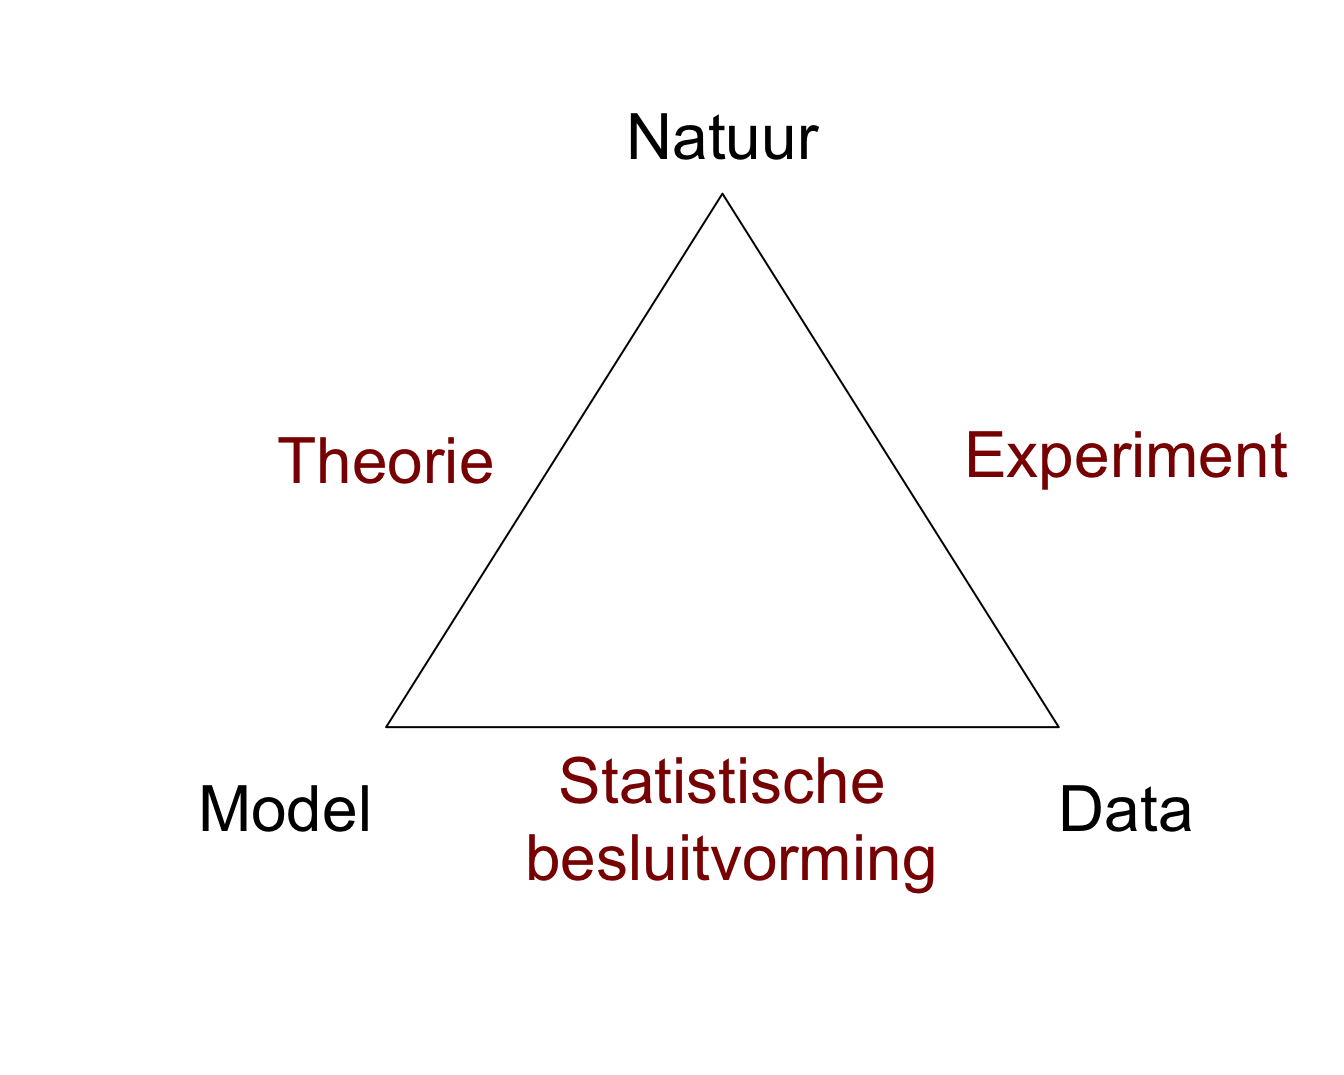
\includegraphics[width=1\linewidth]{Statistiek_2019_2020_files/figure-latex/wetMet-1} 

}

\caption{De Wetenschappelijke Methode en de rol van Statistiek.}\label{fig:wetMet}
\end{figure}

Een andere belangrijke rol van de Statistiek die verder in deze cursus
wordt behandeld, is om de \emph{reproduceerbaarheid} van
wetenschappelijk onderzoek te waarborgen, binnen zelf gekozen
probabiliteitsgrenzen (onzekerheid / zekerheid).

\section{Voorbeeld: Horizon - Homeopathy the
test}\label{voorbeeld-horizon---homeopathy-the-test}

BBC reportage over homeopathie
\url{https://www.dailymotion.com/video/x19idby}

\subsection{\texorpdfstring{Wetenschappelijke hypothese (fragmenten 1-2:
0'00'`-6'00'`\&
7'40'`-11'30'')}{Wetenschappelijke hypothese (fragmenten 1-2: 0'00'-6'00\& 7'40-11'30')}}\label{wetenschappelijke-hypothese-fragmenten-1-2-000-600-740-1130}

Dr.~J. Benveniste was een bekende Franse immunoloog die basofiele
granulocyten, een soort van witte bloedcellen, bestudeerde. Basofiele
granulocyten, ook wel basofielen genoemd, hebben verscheidene
Immunoglobuline E (IgE)-receptoren op het membraan die antigenen kunnen
binden. Als dit type van granulocyten in contact komen met allergenen
dan worden ze geactiveerd en laten hun granules vrij, wat uiteindelijk
kan leiden tot een allergische reactie. Benveniste ontwikkelde een test
waarbij hij de actieve en inactieve basofielen kon onderscheiden aan de
hand van een kleurreactie. Hierdoor kon hij allergische reacties
opsporen door het aantal gekleurde basofielen (diegene die de granules
vrijgelaten hebben) in een staal te tellen en te vergelijken met een
controle staal. Een onderzoeker in zijn labo deed echter eigenaardige
bevindingen. Heel hoge verdunningen van anti-IgE antilichamen activeert
de degranulatie van humane basofielen, een bevinding die het
werkingsmechanisme van homeopathie lijkt te ondersteunen.

Om deze laatste bevinding te testen, pakten Dr.~Benveniste en zijn team
het onderzoek aan volgens de principes van de wetenschappelijke methode.

\begin{itemize}
\tightlist
\item
  Een nieuwe hypothese werd geponeerd: \emph{The Memory of Water}.
\item
  Deductie: Als een substantie van anti-IgE antilichamen sterk wordt
  verdund en heftig wordt geschud, dan wordt de informatie overgedragen
  naar het water zodat een reactie kan worden gedetecteerd door de
  allergietest met gemodificeerde basofielen bij extreem grote
  verdunningen.
\item
  Zet een nieuw experiment op om ``Memory of Water''-hypothese te
  evalueren
\item
  Verken, analyseer en interpreteer de resultaten uit het experiment
\item
  Verspreiden van resultaten
\end{itemize}

Hun werk verscheen in Nature, \citet{benveniste1988}, met een
``Editorial Reservation: Readers of this article may share the
incredulity of the many referees who have commented on several versions
of it during the past several months. The essence of the result is that
an aqueous solution of an antibody retains its ability to evoke a
biological response even when diluted to such an extent that there is a
negligible chance of there being a single molecule in any sample. There
is no physical basis for such an activity. With the kind collaboration
of Professor Benveniste, Nature has therefore arranged for independent
investigators to observe repetitions of the experiments. A report of
this investigation will appear shortly.''

\subsection{Onderzoek dient reproduceerbaar te zijn. Wat ging er fout?
(Fragment:
14'50''-18'56'')}\label{onderzoek-dient-reproduceerbaar-te-zijn.-wat-ging-er-fout-fragment-1450-1856}

Een week na publicatie bezocht een team bestaande uit Nature editor Sir
John Maddox, een wetenschappelijke fraudebuster Walter W. Stewart en
goochelaar en scepticus James Randi, het labo van Benveniste zodat hij
zijn resultaten kon reproduceren onder gecontroleerde contities. Tijdens
een eerste drie pogingen kon het team van Benveniste de resultaten
reproduceren en werd hoge activiteit van de basofielen bevestigd wanneer
ze in contact werden gebracht met de extreem sterk verdunde substantie.

Dr.~Stewart merkte op dat de onderzoekers die de tellingen verrichten,
wisten welke stalen behandeld werden met de controle en welke met de
extreem verdunde substantie. En hij stelde een dubbelgeblindeerde
proefopzet voor, waarbij geen van de onderzoekers wist welke stalen de
controle en welke de behandelde stalen waren. De stalen werden in een
aparte geblindeerde kamer voorbereid en gerandomiseerd. De codes werden
aan het plafond van het lab geplakt. Onder deze meer rigoureuze
procedure kon het team van Benveniste de resultaten niet langer
reproduceren.

Wat ging er fout?

\begin{itemize}
\tightlist
\item
  Proefopzet: Bias kan worden geïntroduceerd als de wetenschapper weet
  hoe de stalen worden behandeld.
\end{itemize}

Oplossing?

\begin{itemize}
\tightlist
\item
  \emph{Blindering (``Blinding'')}

  \begin{itemize}
  \tightlist
  \item
    At random codes toe te wijzen aan de stalen
  \item
    De codes worden gebroken nadat alle data is gecollecteerd
  \item
    Hoe subjectiever de meting hoe belangrijker blindering is
  \end{itemize}
\item
  \emph{Dubbele blindering (``Double blinding''):} Zowel proefpersoon
  als wetenschapper weten niet welke behandeling er werd gegeven
\item
  \emph{Dubbelgeblindeerde} proeven zijn de standaard in
  geneesmiddelenonderzoek. Het is immers nooit voldoende om enkel een
  nieuw middel aan een aantal patiënten toe te dienen om de werkzaamheid
  te evalueren. Er moet steeds een controlegroep zijn die geen werkzaam
  geneesmiddel krijgt, maar een placebo, zodat de effecten daarvan
  kunnen worden vergeleken met die van het ``effectieve'' middel. Men
  heeft dan ook als doel om te bewijzen dat een stof beter werkt dan het
  \emph{placebo-effect}. Cruciaal hierbij is dat de arts die het middel
  voorschrijft, de arts die het effect beoordeelt noch de patiënt mogen
  weten wie de effectieve behandeling kreeg en wie het placebo kreeg.
  Dit om te vermijden dat de artsen hun eigen verwachtingen over het
  middel onbewust aan de patiënt over zouden dragen, of dat het oordeel
  van de artsen over de toestand van de patiënt na de behandeling
  beïnvloed zou worden (vb Fragment: 19'00''-20'30``).
\end{itemize}

\textbf{Dit voorbeeld wijst dus op het belang van een goeie controle!}

\subsection{The ultimate test - proefopzet (Fragment
31'00-39'30'')}\label{the-ultimate-test---proefopzet-fragment-3100-3930}

``The Memory of Water'' hypothese duikt nog geregeld op in de
wetenschappelijke literatuur. Telkens betreft het echter onderzoek met
gebrekkige controles of kon het onderzoek niet gereproduceerd worden.
James Randy speelt met zijn ``one-million-dollar-challenge'' in op deze
onderzoeken. Als scepticus looft hij een prijs uit voor eenieder die
onder gecontroleerde condities claims hard kan maken die volgens de
huidige wetenschappelijk kennis onmogelijk zijn.

Het team van Horizon gaat de ``one-million-dollar-challenge'' aan. Onder
goedkeuring van James Randy zetten zij de volgende proef op om de ``The
Memory of Water'' hypothese te onderzoeken. Een stockoplossing van
actieve stof en een negatieve controle worden aangemaakt en ondergaan
dezelfde stappen. Om mogelijke contaminatie effecten uit te sluiten
worden ze beiden verdund. Eerst worden 2 x 5 proefbuizen met verdunning
van 5C (5 opeenvolgende verdunningen van 1 op 100) gemaakt: 5 met
actieve stof en 5 met puur water. Deze 10 tubes worden random gelabeld.
Hier wordt dus wel op een effectieve manier gebruik gemaakt van
blinding. Na het labelen volgt een verdere verdunning tot 18C.
Vervolgens worden de stalen herlabeld om alle fraude te voorkomen en
worden de stalen naar twee onafhankelijke labo's gestuurd (Marion en
Wayne). In het labo voegen de onderzoekers de humane basofiel
granulocyten toe. Via flowcytometrie, een objectievere meting dan
manuele tellingen, wordt nagegaan hoeveel cellen zijn geactiveerd. De
labo's werd meegedeeld dat er 20 actieve en 20 placebo oplossingen zijn
om te voorkomen dat alle stalen als niet actief worden geklasseerd.
Hierna geeft elk labo zijn ruwe flowcytometrie metingen, proportie
actieve cellen per staal en klassering van de stalen door.

\subsection{The ultimate test - data analyse (Fragment
39'30-43'00'')}\label{the-ultimate-test---data-analyse-fragment-3930-4300}

Nadat alle labo analyses zijn uitgevoerd, verzamelen alle
wetenschappers, journalisten en James Randy zich in ``the Royal
Society''. Een statisticus analyseert de gegevens. Bij het verkennen van
de data, ook de \emph{data exploratie} genoemd, bleken bepaalde stalen
meer activiteit te vertonen dan anderen. De vraag is of dit systematisch
het geval is voor ``sterk-verdunde'' stalen.

In het Marion labo werden 9 proefbuizen van extreme verdunning (D) en 11
van de controles (C) negatief gelabeld. Omdat onderzoekers wisten dat er
20 actieve proefbuizen (D) en 20 controle proefbuizen (C) waren, weten
we ook dat er 11 (D) en 9 (C) stalen als positief werden gelabeld.

\begin{table}[t]

\caption{\label{tab:kruistabelMarion}Kruistabel van de resultaten in het lab van Marion. 11/20 proefbuizen van extreme verdunning (D) en 9/20 van de controles (C) worden als actief gelabeld.}
\centering
\begin{tabular}{lrrr}
\toprule
  & negatief & postief & totaal\\
\midrule
sterk verdund (D) & 9 & 11 & 20\\
controle (C) & 11 & 9 & 20\\
totaal & 20 & 20 & 40\\
\bottomrule
\end{tabular}
\end{table}

\textbf{Falsificatie-principe}: Het is niet mogelijk om een hypothese te
bewijzen met empirische data. We kunnen dus niet aan tonen dat het
effect van D anders is dan van C. We kunnen wel het omgekeerde proberen
te ontkrachten: C en D hebben eenzelfde effect. Als C en D eenzelfde
effect hebben verwachten we dat er evenveel extreem-verdunde stalen als
controle stalen als actief worden gelabeld.

\begin{table}[t]

\caption{\label{tab:kruistabelTheo}Kruistabel van verwachte resultaten als er geen effect is van de verdunning.}
\centering
\begin{tabular}{lrrr}
\toprule
  & negatief & postief & totaal\\
\midrule
sterk verdund (D) & 10 & 10 & 20\\
controle (C) & 10 & 10 & 20\\
totaal & 20 & 20 & 40\\
\bottomrule
\end{tabular}
\end{table}

Enerzijds zou men in het experiment een lichte aanwijzing kunnen zien
dat er in de stalen met extreme verdunning activiteit is: 11/20 stalen
werden correct geklasseerd. Anderzijds, zou het kunnen dat de 11/20
berust op toeval. Als er geen effect is van D zal men door toeval toch
resultaten vinden die lichtjes afwijken van 10/20. Maar hoeveel is
``lichtjes'': 11/20? 12/20? 13/20? \ldots{}

\emph{Hoeveel correcte positieve tests \(x\) zijn er nodig om voldoende
bewijskracht te hebben voor werking van D?} We kunnen dit onderbouwen
met kans om ten minste \(x\) correcte positieve tests te vinden door
zuiver toeval wanneer D niet verschilt van C.
\[p=P(\text{ten minste } x \text{ correcte positieve tests} \vert \text{effect D= effect C})\]

Dergelijke kansen kunnen worden berekend door gebruik te maken van
probabiliteitstheorie (Tabel \ref{tab:pValTableH1}):

\begin{Shaded}
\begin{Highlighting}[]
\NormalTok{knitr}\OperatorTok{::}\KeywordTok{kable}\NormalTok{(}\KeywordTok{cbind}\NormalTok{(}\DataTypeTok{x=}\DecValTok{11}\OperatorTok{:}\DecValTok{15}\NormalTok{,}
  \DataTypeTok{p=}\KeywordTok{phyper}\NormalTok{(}\DataTypeTok{q=}\DecValTok{10}\OperatorTok{:}\DecValTok{14}\NormalTok{,}\DataTypeTok{m=}\DecValTok{20}\NormalTok{,}\DataTypeTok{n=}\DecValTok{20}\NormalTok{,}\DataTypeTok{k=}\DecValTok{20}\NormalTok{,}\DataTypeTok{lower.tail=}\OtherTok{FALSE}\NormalTok{)), tableType,}
  \DataTypeTok{caption =} \StringTok{'Kans op tenminste $x$ correct geklasseerde "sterk-verdunde" stalen wanneer er in werkelijkheid geen effect is.'}\NormalTok{,}
  \DataTypeTok{booktabs =} \OtherTok{TRUE}\NormalTok{,}\DataTypeTok{digits=}\DecValTok{4}
\NormalTok{)}
\end{Highlighting}
\end{Shaded}

\begin{table}[t]

\caption{\label{tab:pValTableH1}Kans op tenminste $x$ correct geklasseerde "sterk-verdunde" stalen wanneer er in werkelijkheid geen effect is.}
\centering
\begin{tabular}{rr}
\toprule
x & p\\
\midrule
11 & 0.3762\\
12 & 0.1715\\
13 & 0.0564\\
14 & 0.0128\\
15 & 0.0019\\
\bottomrule
\end{tabular}
\end{table}

\begin{itemize}
\tightlist
\item
  Als er geen verschil is tussen C en D, dan zal men in 37.6\% van de
  experimenten door toeval een \(x\) observeren van minstens 11
\item
  Het experiment geeft dus absoluut geen bewijs voor de werking van de
  verdunning D.
\end{itemize}

De random variabiliteit in experimenten wordt ook geïllustreerd als we
de resultaten van het Marion labo vergelijken met deze van Wayne (zie
Tabel \ref{tab:kruistabelWayne}).

\begin{table}[t]

\caption{\label{tab:kruistabelWayne}Kruistabel van de resultaten in het lab van Wayne. 9/20 proefbuizen van extreme verdunning (D) en 11/20 van de controles (C) worden als actief gelabeld.}
\centering
\begin{tabular}{lrrr}
\toprule
  & negatief & postief & totaal\\
\midrule
sterk verdund (D) & 11 & 9 & 20\\
controle (C) & 9 & 11 & 20\\
totaal & 20 & 20 & 40\\
\bottomrule
\end{tabular}
\end{table}

Bijgevolg zien we dat we op basis van empirische gegevens nooit met
100\% zekerheid conclusies kunnen trekken. De gegevens zijn onderhevig
aan random variabiliteit en bijgevolg zijn onze conclusies dat ook.

\subsection{Mogelijke fouten}\label{mogelijke-fouten}

\begin{itemize}
\tightlist
\item
  Een experiment is onderhevig aan random variabiliteit bijgevolg zijn
  de conclusies dat ook.
\item
  Zelfs als D en C equivalent zijn, kan men 15 correcte positieve
  resultaten observeren door toeval. Dat kunnen we in 2 op de 1000
  experimenten verwachten.
\item
  In dergelijke steekproef zal men ten onrechte besluiten dat er bewijs
  is voor de werking van D terwijl er in realiteit geen verschil is
  tussen D en C.\\
\item
  Intuïtief voelen we aan dat we niet met absolute zekerheid uitspraken
  kunnen doen over populatiekarakteristieken op basis van een eindige
  steekproef.
\end{itemize}

In deze cursus zullen we daarom steeds volgende facetten van de
statistiek bespreken:

\begin{itemize}
\tightlist
\item
  \emph{Proefopzet}: hoe zijn de gegevens tot stand gekomen
\item
  \emph{Data exploratie en beschrijvende statistiek}: exploreren,
  visualiseren, samenvatten en beschrijven van geobserveerde data zodat
  relevante aspecten naar voor komen.
\item
  \emph{Statistische besluitvorming}: aan de hand van statistische
  modellen bestuderen in hoeverre geobserveerde trends/effecten die
  geobserveerd worden in een steekproef veralgemeend kunnen worden naar
  de algemene populatie.
\end{itemize}

\chapter{Belangrijke concepten \&
conventies}\label{belangrijke-concepten-conventies}

De verschillende stappen in een studie worden geïllustreerd in Figuur
\ref{fig:pop2Samp2Pop}. Eerst bepaalt de onderzoeker de \emph{populatie}
van interesse. Gezien het om financiële en logistieke beperkingen
vrijwel nooit mogelijk is om de volledige populatie te onderzoeken zal
men vervolgens een steekproef nemen uit de populatie. De manier waarop
een steekproef zal worden genomen wordt vastgelegd in het \emph{design
van de studie}. \emph{Proefopzet} of \emph{studie design} is een aparte
tak van de statisitiek en is een cruciaal onderdeel van een studie. Het
studie design moet immers garanderen dat de gegevens en resultaten van
de steekproef representatief zijn voor de populatie zodat de resultaten
van de studie veralgemeneend kunnen worden naar de populatie toe.
Vervolgens wordt de studie uitgevoerd, worden de gegevens verzameld en
kan de eigenlijke data-analyse van start gaan. In een eerste fase is het
belangrijk om de gegevens grondig te exploreren. \emph{Data-exploratie
en beschrijvende statistiek} is een tweede tak van de statistiek die
toelaat om gegevens van de steekproef te visualiseren, samen te vatten
en om inzicht in de data te verwerven. Dat is belangrijk om de data
correct te kunnen modelleren en om aannames na te kunnen gaan die nodig
zijn voor de verdere data analyse. Vervolgens zullen we hetgeen we
observeren in de steekproef trachten te veralgemenen naar de algemene
populatie toe, zodat we algemene conclusies kunnen trekken op
populatie-niveau op basis van de steekproef van de studie. Hiervoor zijn
methodes nodig van de \emph{statistische besluitvorming}, ook wel
\emph{statistische inferentie} genoemd, een derde belangrijke tak van de
statistiek.

\begin{figure}

{\centering 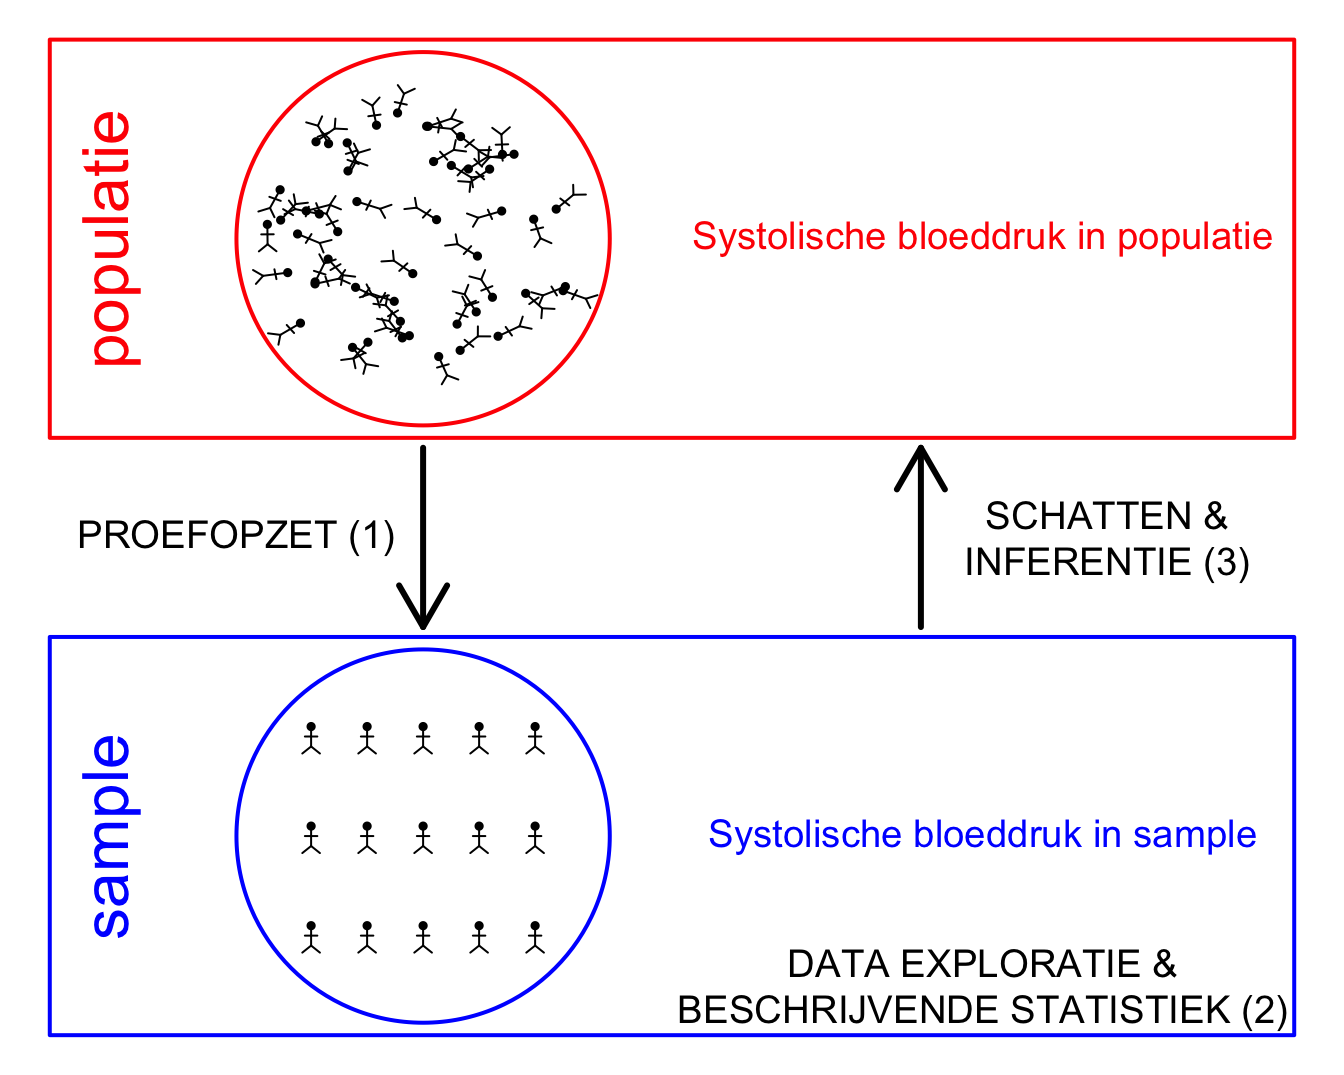
\includegraphics[width=1\linewidth]{Statistiek_2019_2020_files/figure-latex/pop2Samp2Pop-1} 

}

\caption{Verschillende stappen in een studie. (1) In de design fase/ proefopzet definieert de onderzoeker de populatie, bepaalt hij/zij op welke manier een steekproef zal worden genomen uit de populatie en hoe het experiment zal worden uitgevoerd. Ook het volledige data analyse plan moet in deze fase zijn vastgelegd. Vervolgens wordt het experiment uitgevoerd en worden de gegevens verzameld. (2) De gegevens worden vervolgens verkend en samengevat. Hierbij verwerft men inzicht in de gegevens en kunnen aannames worden nagegaan die noodzakelijk zijn voor de verdere data analyse stappen. (3) Tenslotte zal men hetgeen men observeert in de steekproef trachten te veralgemenen naar de populatie toe a.d.h.v. statistische inferentie.}\label{fig:pop2Samp2Pop}
\end{figure}

Vooraleer we dieper ingaan op studie-design, data-exploratie en
statistische besluitvorming zullen we eerst enkele concepten
introduceren. We doen dat in dit hoofdstuk aan de hand van de de NHANES
studie.

\BeginKnitrBlock{example}[NHANES studie]
\protect\hypertarget{exm:nhanesExConcepten}{}{\label{exm:nhanesExConcepten}
\iffalse (NHANES studie) \fi{} }
\EndKnitrBlock{example}

De National Health and Nutrition Examination Survey (NHANES) wordt sinds
1960 op regelmatige basis afgenomen. In dit voorbeeld maken we gebruik
van de gegevens die werden verzameld tussen 2009-2012 bij 10000
Amerikanen en die werden opgenomen in het R-pakket NHANES. Er werd een
groot aantal fysieke, demografische, nutritionele, levelsstijl en
gezondheidskarakteristieken gecollecteerd in deze studie (zie Tabel
\ref{tab:nhanesConcepten}). \texttt{**Einde\ voorbeeld**}

\begin{table}[t]

\caption{\label{tab:nhanesConcepten}Overzicht van een aantal variabelen uit de NHANES studie.}
\centering
\begin{tabular}{rlrlrrrrrll}
\toprule
ID & Gender & Age & Race1 & Weight & Height & BMI & BPSysAve & TotChol & SmokeNow & Smoke100\\
\midrule
51624 & male & 34 & White & 87.4 & 164.7 & 32.22 & 113 & 3.49 & No & Yes\\
51625 & male & 4 & Other & 17.0 & 105.4 & 15.30 & NA & NA & NA & NA\\
51630 & female & 49 & White & 86.7 & 168.4 & 30.57 & 112 & 6.70 & Yes & Yes\\
51638 & male & 9 & White & 29.8 & 133.1 & 16.82 & 86 & 4.86 & NA & NA\\
51646 & male & 8 & White & 35.2 & 130.6 & 20.64 & 107 & 4.09 & NA & NA\\
\addlinespace
51647 & female & 45 & White & 75.7 & 166.7 & 27.24 & 118 & 5.82 & NA & No\\
\bottomrule
\end{tabular}
\end{table}

\section{Variabelen}\label{variabelen}

Een \emph{variabele} is een karakteristiek (bvb. Systolische bloeddruk,
leeftijd, geslacht, \ldots{}) die varieert van subject tot subject (bvb.
van persoon tot persoon, van dier tot dier, \ldots{}) in de studie. Er
zijn verschillende \emph{types} variabelen.

\emph{Kwalitatieve variabelen} hebben (meestal) beperkt aantal
uitkomstcategorieën die niet numeriek van aard zijn. Deze worden
onderverdeeld in \emph{nominale variabelen} en \emph{ordinale
variabelen} . Nominale gegevens zijn er die men kan benoemen. Ze worden
niet gemeten en kennen geen natuurlijke ordening; bijvoorbeeld geslacht,
ras, bloedgroep, kleur van ogen, \ldots{} Ordinale variabelen kennen wel
een ordening; bijvoorbeeld de BMI klasse volgens het WHO, de
rokersstatus (nooit gerookt, ooit gerookt maar gestopt, actueel roker),
\ldots{}

Een ander type van variabelen zijn \emph{numerieke variabelen}. Hierbij
maakt men het onderscheid tussen \emph{numerieke discrete variabelen} en
\emph{numerieke continue variabelen}. Numerieke discrete variabelen
bestaan uit tellingen, b.v. het aantal partners die men had gedurende
het leven (geregistreerd in de NHANES studie), het aantal salamanders
van de species \textbf{P. jordani} in een bepaald gebied, het aantal
reads dat mapt op een bepaald gen in een genexpressiestudie waarbij men
gebruik maakt van next-generation sequencing technologie , \ldots{}

Numerieke continue variabelen kunnen (tenminste in theorie) tussen
bepaalde grenzen elke mogelijke waarde aannemen. Bijvoorbeeld, leeftijd
is continu want het verschil in leeftijd tussen 2 personen kan in
principe willekeurig klein zijn (1 uur, 1 minuut, \ldots{}). Analoog
zijn het gewicht, BMI, fluorescentie-metingen in een ELISA experiment,
\ldots{} continue metingen.

In de wetenschappen gaat men vaak continue gegevens dichotomiseren om ze
nominaal te maken. Bijvoorbeeld, systolische bloeddruk wordt omgezet in
hypertensie (\(>140\) mmHg) en normotensie (\(\leq 140\) mmHg). Dit
vereenvoudigt de beschrijving van gegevens. Helaas is dit een slechte
praktijk omdat het meestal leidt tot een aanzienlijk verlies aan
informatie en omdat de aldus bekomen resultaten sterk afhankelijk kunnen
zijn van de gekozen drempelwaarde. In de praktijk worden de uitkomsten
van continue variabelen ook vaak afgerond zodat de vermelde waarden in
feite discreet zijn. Om analoge redenen is het vaak wenselijk om ze als
continue variabelen te blijven beschouwen.

In de praktijk wil men vaak numerieke rangen toekennen aan de
verschillende waarden die ordinale variabelen aannemen. Bijvoorbeeld kan
men ervoor kiezen de codes 1, 2 en 3 toe te kennen aan de meetwaarden
\emph{nooit gerookt}, \emph{ooit gerookt maar gestopt} en \emph{actueel
roker}. Het is belangrijk om te beseffen dat de keuze van die numerieke
waarden vaak geen betekenis heeft. Het verschil tussen de toegekende
codes (3-2=1, 2-1=1, 3-2=1) is niet bruikbaar gezien men bijvoorbeeld
niet onderstellen dat de wijziging in rokerstatus identiek is van
\emph{nooit gerookt} naar \emph{ooit gerookt maar gestopt} (2-1=1) en
van \emph{ooit gerookt maar gestopt} naar \emph{actueel roker} (3-2=1).

\BeginKnitrBlock{example}[oefening]
\protect\hypertarget{exm:unnamed-chunk-3}{}{\label{exm:unnamed-chunk-3}
\iffalse (oefening) \fi{} }Geef het type aan van de variabelen in Tabel
\ref{tab:nhanesConcepten}
\EndKnitrBlock{example}

\section{Populatie}\label{subsec:pop}

Het doel van een wetenschappelijke studie is nagenoeg altijd om
uitspraken te doen over de algemene populatie. Stel bijvoorbeeld dat men
een grenswaarde wil afleiden om patiënten met hypertensie op te sporen.
Hiervoor zal men eerst de systolische bloeddruk moeten bestuderen bij
een populatie van gezonde personen. Een populatie is meestal continu in
verandering. Bovendien is men meestal niet alleen geïnteresseerd in
effecten bij huidige subjecten, maar ook in het effect bij toekomstige
subjecten. De populatie kan dus als oneindig groot worden beschouwd en
is op een bepaald ogenblik zelfs niet volledig observeerbaar\footnote{B.v.
  omdat het ook toekomstige subjecten omvat}. De populatie kan binnen de
statistiek dus worden opgevat als een theoretisch concept die alle
huidige en toekomstige subjecten omvat waarover men uitspraken wenst te
doen. In de praktijk zal men dus nooit de volledige populatie kunnen
bemonsteren en dient men een steekproef te nemen van de populatie. Om
een representatieve groep subjecten te waarborgen, vertrekt een goede
onderzoeksopzet vanuit een belangrijke, precies geformuleerde
vraagstelling omtrent een duidelijk omschreven populatie. Vaak worden
hierbij inclusie- en exclusiecriteria geformuleerd.

\emph{Inclusiecriteria} zijn karakteristieken die een
subject/experimentele eenheid moet hebben om tot de populatie te
behoren, b.v.

\begin{itemize}
\tightlist
\item
  specifieke ziekte: hypertensie
\item
  leeftijdscategorie
\item
  geslacht
\item
  \ldots{}
\end{itemize}

\emph{Exclusiecriteria} zijn karakteristieken die een
subject/experimentele eenheid niet mag hebben om tot de populatie te
behoren, b.v.

\begin{itemize}
\tightlist
\item
  geneesmiddelen gebruik
\item
  andere ziekten
\item
  zwangerschap
\item
  \ldots{}
\end{itemize}

Op de subjecten zal men meestal een aantal karakteristieken meten, ook
wel \emph{variabelen} genoemd (bvb. Systolische bloeddruk, leeftijd,
geslacht, \ldots{}). Typisch zullen deze variabelen variëren van subject
tot subject (bvb. van persoon tot persoon, van dier tot dier, \ldots{})
in de populatie.

\section{Toevalsveranderlijken (of toevallige
veranderlijken)}\label{toevalsveranderlijken-of-toevallige-veranderlijken}

De belangrijke vraag, waar we in in de verdere hoofdstukken dieper op in
zullen gaan, is hoe nauwkeurig we uitspraken kunnen doen over de
populatie o.b.v. een groep gemeten subjecten in een steekproef. De
spreiding op de gegevens zal daar een cruciale rol in spelen. Als de
gegevens niet variëren tussen subjecten, dan zullen alle steekproeven
uit de populatie hetzelfde resultaat opleveren en zullen de bekomen
schattingen niet afwijken van de gezochte populatieparameters. Als
daarentegen de gegevens zeer chaotisch zijn, dan zullen verschillende
steekproeven mogelijks zeer verschillende resultaten opleveren, die
bijgevolg ver kunnen afwijken van de gezochte populatieparameters.

Om het denkwerk te vergemakkelijken, zullen we hoofdletters gebruiken om
aan te geven dat de bestudeerde karakteristiek (vb. een meetresultaat
zoals systolische bloeddruk) variabel is in de populatie, zonder daarbij
concreet over de gerealiseerde waarde voor een bepaald subject na te
denken. Dergelijke meting of variabele \(X\) wordt algemeen een
\emph{toevalsveranderlijke} of \emph{toevallige veranderlijke} genoemd,
(a) omdat ze formeel het resultaat aanduidt van een \emph{toevallige
trekking} van een bepaalde karakteristiek uit de studiepopulatie en (b)
omdat ze bovendien \emph{veranderlijk} is, niet alle subjecten in de
steekproef bezitten immers dezelfde waarde voor die karakteristiek.

Het makkelijkst om over een toevalsveranderlijke \(X\) na te denken is
alsof \(X\) het label voorstelt van een bepaalde populatiekarakteristiek
voor een lukraak individu uit de bestudeerde populatie, vooraleer haar
concrete waarde gemeten werd. Met andere woorden, een
toevalsveranderlijke \(X\) kan men opvatten als onbekende veranderlijke
die een meting voorstelt die we plannen te verzamelen, maar nog niet
hebben verzameld. Net zoals observaties kunnen we toevallig
veranderlijken klasseren als kwalitatief, kwantitatief, discreet,
continu, \ldots{}.

\section{Beschrijven van de
populatie}\label{beschrijven-van-de-populatie}

Voor we een random variabele meten, kunnen we onmogelijk zeggen hoe hoog
de meting precies zal zijn. De gerealiseerde waarde van \(X\) is dus
onderhevig aan random variabiliteit. Onze geobserveerde steekproef
\(x_1, x_2, . . . , x_{275}\) kan dus als n = 275 realisaties worden
beschouwd van dezelfde random variable X, voor subject \(i\), met
\(i = 1,2,...,275\). Een random veranderlijke, een karakteristiek van de
populatie, wordt beschreven door gebruik te maken van een
\emph{verdeling}.

De verdeling beschrijft de waarschijnlijkheid om een bepaalde waarde te
observeren voor de toevallig veranderlijke wanneer men volledige lukraak
een proefpersoon kiest uit de populatie. De densiteitsfunctie van de
verdeling wordt vaak genoteerd als f(X). Heel vaak volgen biologische en
chemische data een Normale verdeling. De Normale verdeling is een
theoretische verdeling met een klokvorm die volledig gedefineerd wordt
door twee parameters, het gemiddelde \(\mu\) en de variantie
\(\sigma^2\). We zullen in latere hoofdstukken dieper ingaan op de
normale verdeling.

Veronderstel bijvoorbeeld dat de gemiddelde bloeddruk van subjecten in
de populatie van gezonde 40-65 jarigen gelijk is aan \(\mu=120\) mmHg en
de variantie \(\sigma^2=196\). De verdeling van de systolische bloeddruk
wordt weergegeven in Figuur \ref{fig:nhanesNormal} die d.m.v.
onderstaande code wordt gegenereerd in R.

\begin{Shaded}
\begin{Highlighting}[]
\NormalTok{grid <-}\StringTok{ }\KeywordTok{seq}\NormalTok{(}\DecValTok{65}\NormalTok{, }\DecValTok{175}\NormalTok{, }\FloatTok{0.1}\NormalTok{)}
\KeywordTok{plot}\NormalTok{(grid, }\KeywordTok{dnorm}\NormalTok{(grid, }\DataTypeTok{mean =} \DecValTok{120}\NormalTok{, }\DataTypeTok{sd =} \DecValTok{196}\OperatorTok{^}\FloatTok{0.5}\NormalTok{), }\DataTypeTok{xlab =} \StringTok{"Systolische Bloeddruk (mm kwik)"}\NormalTok{, }
    \DataTypeTok{col =} \DecValTok{2}\NormalTok{, }\DataTypeTok{ylab =} \StringTok{"Densiteit"}\NormalTok{, }\DataTypeTok{type =} \StringTok{"l"}\NormalTok{, }\DataTypeTok{lwd =} \DecValTok{2}\NormalTok{)}
\NormalTok{grid2 <-}\StringTok{ }\KeywordTok{seq}\NormalTok{(}\DecValTok{115}\NormalTok{, }\DecValTok{120}\NormalTok{, }\FloatTok{0.01}\NormalTok{)}
\KeywordTok{polygon}\NormalTok{(}\DataTypeTok{x =} \KeywordTok{c}\NormalTok{(grid2, }\DecValTok{120}\NormalTok{, }\DecValTok{115}\NormalTok{), }\DataTypeTok{y =} \KeywordTok{c}\NormalTok{(}\KeywordTok{dnorm}\NormalTok{(grid2, }
    \DecValTok{120}\NormalTok{, }\DecValTok{196}\OperatorTok{^}\FloatTok{0.5}\NormalTok{), }\DecValTok{0}\NormalTok{, }\DecValTok{0}\NormalTok{), }\DataTypeTok{col =} \DecValTok{2}\NormalTok{, }\DataTypeTok{border =} \DecValTok{2}\NormalTok{)}
\KeywordTok{text}\NormalTok{(}\DecValTok{120}\NormalTok{, }\KeywordTok{dnorm}\NormalTok{(}\DecValTok{120}\NormalTok{, }\DecValTok{120}\NormalTok{, }\DecValTok{196}\OperatorTok{^}\FloatTok{0.5}\NormalTok{), }\KeywordTok{paste0}\NormalTok{(}\StringTok{"P(115 < X < 120) ="}\NormalTok{, }
    \KeywordTok{round}\NormalTok{(}\KeywordTok{diff}\NormalTok{(}\KeywordTok{pnorm}\NormalTok{(}\KeywordTok{c}\NormalTok{(}\DecValTok{115}\NormalTok{, }\DecValTok{120}\NormalTok{), }\DecValTok{120}\NormalTok{, }\DecValTok{196}\OperatorTok{^}\FloatTok{0.5}\NormalTok{)) }\OperatorTok{*}\StringTok{ }
\StringTok{        }\DecValTok{100}\NormalTok{, }\DecValTok{1}\NormalTok{), }\StringTok{"%"}\NormalTok{), }\DataTypeTok{col =} \DecValTok{2}\NormalTok{, }\DataTypeTok{cex =} \DecValTok{1}\NormalTok{, }\DataTypeTok{pos =} \DecValTok{4}\NormalTok{)}
\end{Highlighting}
\end{Shaded}

\begin{figure}

{\centering 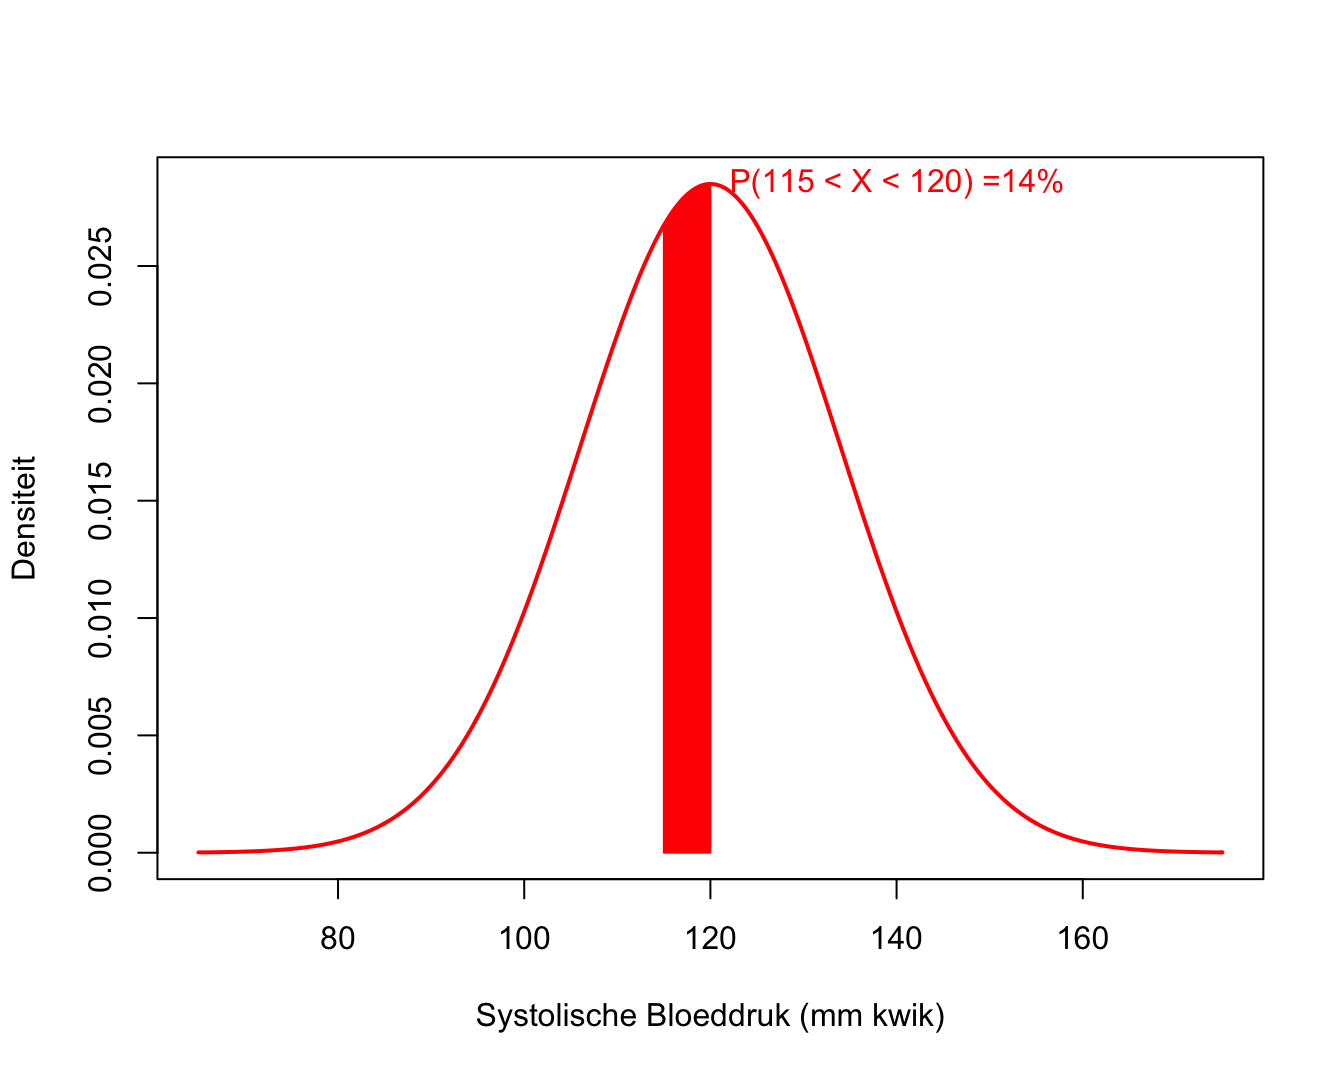
\includegraphics[width=1\linewidth]{Statistiek_2019_2020_files/figure-latex/nhanesNormal-1} 

}

\caption{Normale verdeling voor de systolische bloeddruk van gezonde personen tussen 40-65 jaar met gemiddelde 120 mm Hg en variantie 196.}\label{fig:nhanesNormal}
\end{figure}

Op basis van de verdeling kunnen we kansen berekenen om bijvoorbeeld een
lukraak subject te bemonsteren uit de populatie met een bloeddruk tussen
115 en 120 mmHg. De kansen worden weergegeven door de oppervlakte onder
de densiteitsfunctie:

\[P[115\leq  X\leq 120]= \int\limits_{115}^{120} f(x) dx = 0.14\]

De grafische interpretatie wordt weergegeven in Figuur
\ref{fig:nhanesNormal}. De oppervlakte onder de volledige
densiteitscurve is gelijk aan 1

\[P[-\infty\leq X \leq +\infty]=\int\limits_{-\infty}^{+\infty} f(x) dx=1\]

Kansen liggen uiteraard steeds tussen 0 en 1!

Kansen worden veelal berekend door gebruik te maken van de
\emph{cumulatieve distributie functie} van de verdeling, F(x), m.a.w. de
functie die weergeeft wat de kans is dat een Normaal verdeelde
toevallige veranderlijke een waarde zal aannemen die kleiner of gelijk
is aan de vooropgestelde kwantiel x:
\[F(x)=\int\limits_{-\infty}^x f(x) dx  = P[X\leq x].\]

\begin{center}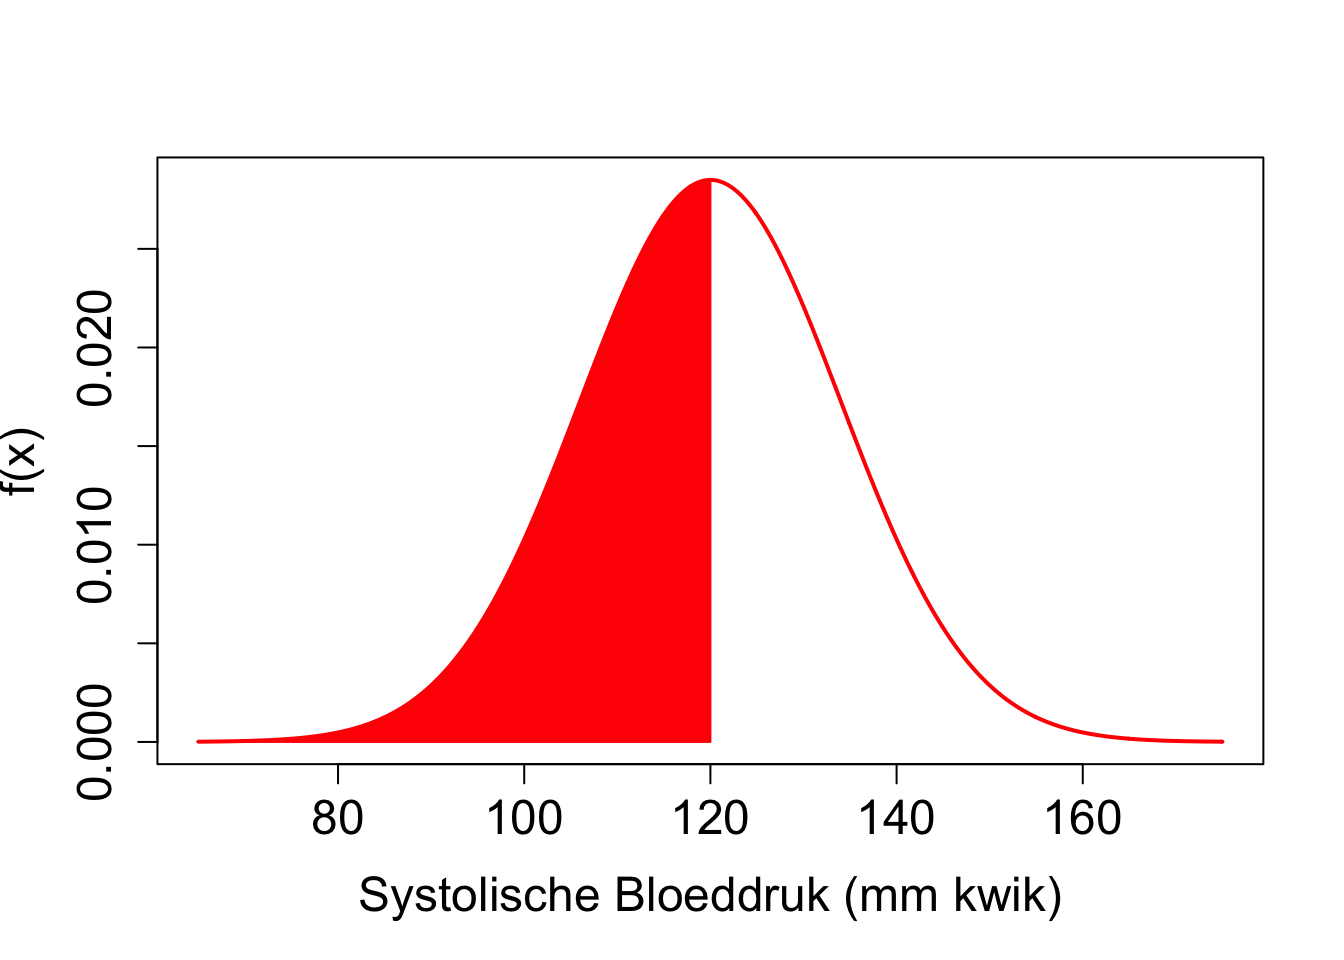
\includegraphics[width=0.6\linewidth]{Statistiek_2019_2020_files/figure-latex/nhanesNormalCum-1} \end{center}

\begin{center}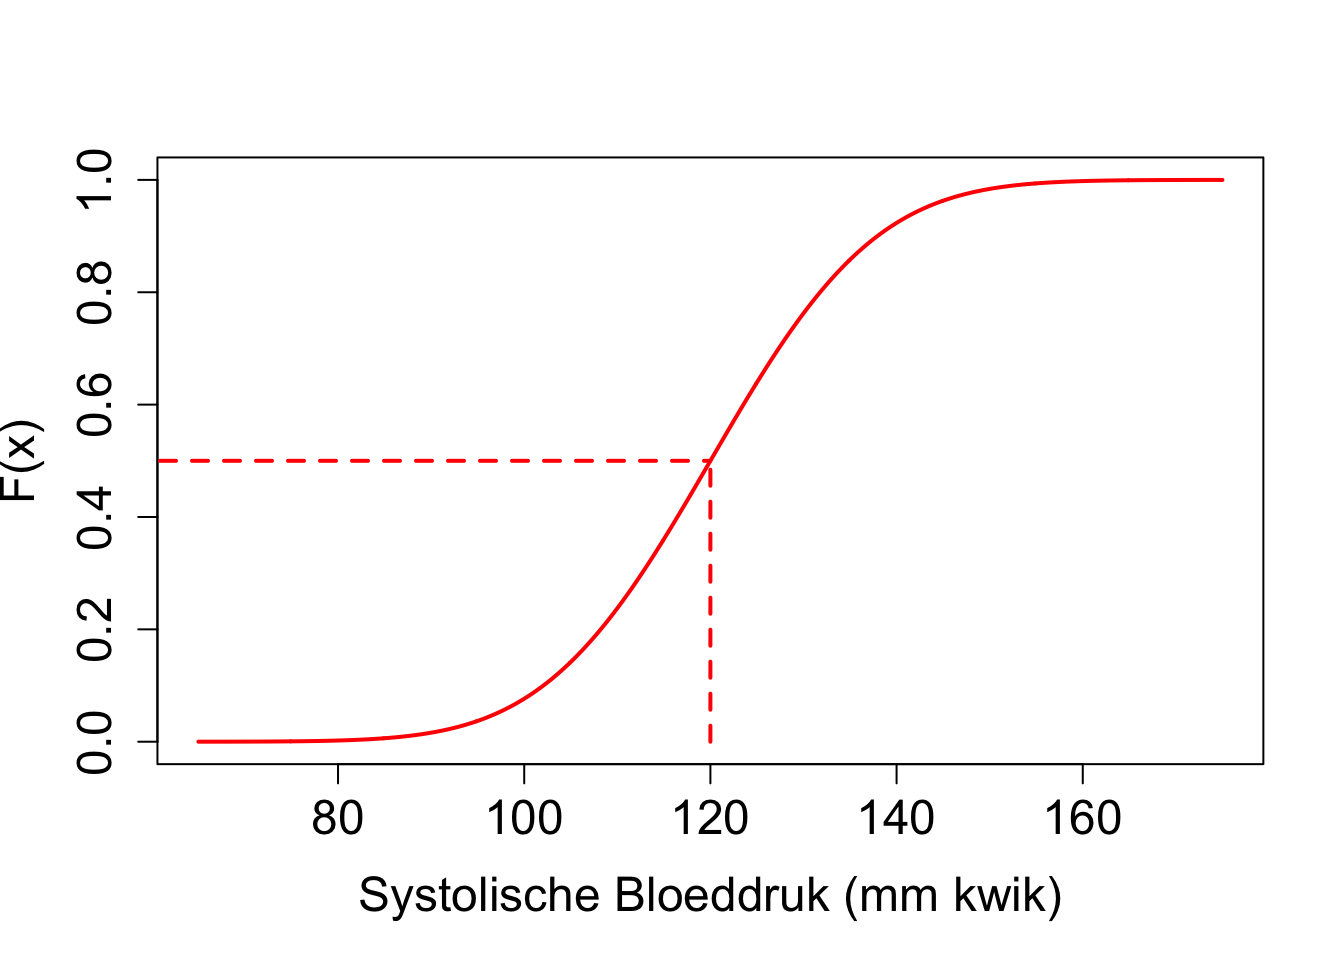
\includegraphics[width=0.6\linewidth]{Statistiek_2019_2020_files/figure-latex/nhanesNormalCum-2} \end{center}

Merk op dat de de normale distributie in R wordt geparameteriseerd
a.d.h.v. het gemiddelde \(\mu\) en de standaard afwijking \(\sigma\). Op
basis van de Normaal verdeling die we veronderstelden voor de
systolische bloeddruk in de populatie \(N(\mu=120\),\(\sigma^2=196)\)
bekomen we

\begin{Shaded}
\begin{Highlighting}[]
\KeywordTok{pnorm}\NormalTok{(}\DecValTok{120}\NormalTok{, }\DataTypeTok{mean =} \DecValTok{120}\NormalTok{, }\DataTypeTok{sd =} \DecValTok{196}\OperatorTok{^}\FloatTok{0.5}\NormalTok{)}
\end{Highlighting}
\end{Shaded}

\begin{verbatim}
## [1] 0.5
\end{verbatim}

\begin{Shaded}
\begin{Highlighting}[]
\KeywordTok{pnorm}\NormalTok{(}\DecValTok{115}\NormalTok{, }\DataTypeTok{mean =} \DecValTok{120}\NormalTok{, }\DataTypeTok{sd =} \DecValTok{196}\OperatorTok{^}\FloatTok{0.5}\NormalTok{)}
\end{Highlighting}
\end{Shaded}

\begin{verbatim}
## [1] 0.3604924
\end{verbatim}

\begin{Shaded}
\begin{Highlighting}[]
\KeywordTok{pnorm}\NormalTok{(}\DecValTok{120}\NormalTok{, }\DataTypeTok{mean =} \DecValTok{120}\NormalTok{, }\DataTypeTok{sd =} \DecValTok{196}\OperatorTok{^}\FloatTok{0.5}\NormalTok{) }\OperatorTok{-}\StringTok{ }\KeywordTok{pnorm}\NormalTok{(}\DecValTok{115}\NormalTok{, }\DataTypeTok{mean =} \DecValTok{120}\NormalTok{, }
    \DataTypeTok{sd =} \DecValTok{196}\OperatorTok{^}\FloatTok{0.5}\NormalTok{)}
\end{Highlighting}
\end{Shaded}

\begin{verbatim}
## [1] 0.1395076
\end{verbatim}

waarbij pnorm de kans berekent dat de bloeddruk bij een willekeurig
subject in de populatie lager of gelijk is aan het kwantiel dat wordt
opgegeven (hier 120 mm Hg en 115 mm Hg). Het verschil tussen beide
kansen geeft dan de kans weer op een bloeddruk tussen 115 en 120 mm Hg.
Let wel dat R de parameterisatie gebruikt van het gemiddelde \(\mu\) en
de standaard afwijking \(\sigma\), ipv de variantie \(\sigma^2\).

In de praktijk kennen we de werkelijke verdeling in de populatie niet en
moet deze worden geschat o.b.v. de steekproef.

\section{Steekproef}\label{steekproef}

In de praktijk is het om financiële en logistieke redenen bijna nooit
mogelijk om de volledige populatie te bestuderen. Populatieparameters
kunnen daarom meestal niet exact bepaald worden. Enkel een deel van de
populatie kan onderzocht worden, hetgeen men de \emph{steekproef} noemt.
Volgens een gestructureerd design worden daartoe \textbf{lukraak
subjecten} uit de doelpopulatie getrokken en geobserveerd. De onbekende
parameters worden vervolgens geschat o.b.v. die steekproef en noemt met
schattingen. In de praktijk hoopt men uiteraard dat de schattingen die
men bekomt op basis van de steekproef vergelijkbaar zijn met de
overeenkomstige populatieparameters die men voor de volledige populatie
zou bekomen.

Stel bijvoorbeeld dat we op basis van de NHANES studie hypertensie
wensen te definiëren. We zullen hiervoor subjecten met ``normale''
bloeddrukwaarden moeten selecteren. Veronderstel dat we \(n\) gezonde
personen zullen selecteren in de studie tussen 40 en 65 jaar en we
geïnteresseerd zijn in systolische bloeddruk. Telkens een lukraak
individu getrokken wordt uit de populatie zal men een realisatie van de
toevalsveranderlijke \(X\) kunnen observeren. Die realisatie of
geobserveerde waarde duiden we aan met een kleine letter \(x\). Deze
stelt dus een welbepaald getal voor en is niet langer een onbekende
veranderlijke zoals \(X\). Samengevat zijn de nog onbekende waarden voor
de bestudeerde populatiekarakteristiek bij subjecten 1 tot \(n\) in de
steekproef, toevalsveranderlijken die we algemeen met \(X_1,...,X_n\)
zullen noteren. Na het trekken van de steekproef, ziet men de
gerealiseerde uitkomsten \(x_1, x_2, \dots, x_n\), bijvoorbeeld hun
gemeten systolische bloeddruk.

We selecteren hieronder de subset van gezonde personen tussen de 40-65
jaar in de NHANES studie. Deze definiëren we verder als niet rokers,
zonder diabetes, met een normaal BMI, zonder historiek van hard drugs,
zonder lage gezondheidsstatus en zonder slaapproblemen. Op deze manier
hebben we dus inclusie- en exclusiecriteria geformuleerd voor het
definiëren van de populatie van interesse.

\begin{Shaded}
\begin{Highlighting}[]
\KeywordTok{library}\NormalTok{(NHANES)}
\NormalTok{NHANES2 =}\StringTok{ }\KeywordTok{subset}\NormalTok{(NHANES, }\OperatorTok{!}\KeywordTok{is.na}\NormalTok{(Race1) }\OperatorTok{&}\StringTok{ }\OperatorTok{!}\KeywordTok{is.na}\NormalTok{(Smoke100n) }\OperatorTok{&}\StringTok{ }
\StringTok{    }\OperatorTok{!}\KeywordTok{is.na}\NormalTok{(BMI_WHO) }\OperatorTok\StringTok{ }\OperatorTok{!}\KeywordTok{is.na}\NormalTok{(Age) }\OperatorTok{&}\StringTok{ }\OperatorTok{!}\KeywordTok{is.na}\NormalTok{(HardDrugs) }\OperatorTok{&}\StringTok{ }
\StringTok{    }\OperatorTok{!}\KeywordTok{is.na}\NormalTok{(HealthGen) }\OperatorTok{&}\StringTok{ }\OperatorTok{!}\KeywordTok{is.na}\NormalTok{(Gender) }\OperatorTok{&}\StringTok{ }\OperatorTok{!}\KeywordTok{is.na}\NormalTok{(AlcoholYear) }\OperatorTok{&}\StringTok{ }
\StringTok{    }\OperatorTok{!}\KeywordTok{is.na}\NormalTok{(BPSys1) }\OperatorTok{&}\StringTok{ }\OperatorTok{!}\KeywordTok{is.na}\NormalTok{(BPSys2) }\OperatorTok{&}\StringTok{ }\OperatorTok{!}\KeywordTok{is.na}\NormalTok{(BPSys3) }\OperatorTok{&}\StringTok{ }
\StringTok{    }\OperatorTok{!}\KeywordTok{is.na}\NormalTok{(SleepTrouble))}
\NormalTok{NHANES2}\OperatorTok{$}\NormalTok{bpSys =}\StringTok{ }\KeywordTok{rowMeans}\NormalTok{(NHANES2[, }\KeywordTok{c}\NormalTok{(}\DecValTok{27}\NormalTok{, }\DecValTok{29}\NormalTok{, }\DecValTok{31}\NormalTok{)])}
\NormalTok{nhanesSub =}\StringTok{ }\KeywordTok{subset}\NormalTok{(NHANES2, Age }\OperatorTok{<=}\StringTok{ }\DecValTok{65} \OperatorTok{&}\StringTok{ }\NormalTok{Age }\OperatorTok{>=}\StringTok{ }\DecValTok{40} \OperatorTok{&}\StringTok{ }
\StringTok{    }\OperatorTok{!}\KeywordTok{duplicated}\NormalTok{(ID))}
\NormalTok{nhanesSubHealthy =}\StringTok{ }\KeywordTok{subset}\NormalTok{(nhanesSub, Smoke100n }\OperatorTok{==}\StringTok{ "Non-Smoker"} \OperatorTok{&}\StringTok{ }
\StringTok{    }\NormalTok{Diabetes }\OperatorTok{==}\StringTok{ "No"} \OperatorTok{&}\StringTok{ }\KeywordTok{as.double}\NormalTok{(BMI_WHO) }\OperatorTok\StringTok{ }\KeywordTok{c}\NormalTok{(}\DecValTok{2}\NormalTok{, }
    \DecValTok{3}\NormalTok{) }\OperatorTok{&}\StringTok{ }\NormalTok{HardDrugs }\OperatorTok{==}\StringTok{ "No"} \OperatorTok{&}\StringTok{ }\NormalTok{HealthGen }\OperatorTok{!=}\StringTok{ "Poor"} \OperatorTok{&}\StringTok{ }
\StringTok{    }\NormalTok{SleepTrouble }\OperatorTok{==}\StringTok{ "No"}\NormalTok{)}
\KeywordTok{head}\NormalTok{(nhanesSubHealthy}\OperatorTok{$}\NormalTok{bpSys)}
\end{Highlighting}
\end{Shaded}

\begin{verbatim}
## [1] 114.00000 140.66667  94.66667 152.66667 128.00000 124.00000
\end{verbatim}

\begin{Shaded}
\begin{Highlighting}[]
\KeywordTok{dim}\NormalTok{(nhanesSubHealthy)}
\end{Highlighting}
\end{Shaded}

\begin{verbatim}
## [1] 275  77
\end{verbatim}

Op basis van de inclusie en exclusie-criteria werden \(n=275\) gezonde
individuen uit de Amerikaanse populatie weerhouden. De toevallig
veranderlijke systolische bloeddruk wordt dus genoteerd als \(X\)
terwijl de n = 275 geobserveerde metingen genoteerd worden als
\(x_1,x_2,...,x_{275}\). De variable \(X\) is random of stochastisch
aangezien zijn waarde veranderlijk is. Voor een random subject uit de
populatie kunnen we de systolische bloeddruk niet exact voorspellen, het
hangt immers af van het geselecteerde subject, tijdstip van de meting,
\ldots{}

\section{Schatten van de verdeling in de
populatie}\label{schatten-van-de-verdeling-in-de-populatie}

In realiteit kennen we de verdeling van de gegevens niet. We kunnen de
verdeling o.b.v. de steekproef schatten en grafisch weergegeven a.d.h.v.
een histogram (functie \texttt{hist()} in R)

\begin{Shaded}
\begin{Highlighting}[]
\NormalTok{histAbs <-}\StringTok{ }\KeywordTok{hist}\NormalTok{(nhanesSubHealthy}\OperatorTok{$}\NormalTok{bpSys, }\DataTypeTok{xlab =} \StringTok{"Systolische Bloeddruk (mm kwik)."}\NormalTok{, }
    \DataTypeTok{breaks =} \KeywordTok{seq}\NormalTok{(}\DecValTok{65}\NormalTok{, }\DecValTok{175}\NormalTok{, }\DecValTok{5}\NormalTok{), }\DataTypeTok{ylab =} \StringTok{"Frequentie"}\NormalTok{, }
    \DataTypeTok{cex.main =} \FloatTok{1.5}\NormalTok{, }\DataTypeTok{cex.axis =} \FloatTok{1.5}\NormalTok{, }\DataTypeTok{cex.lab =} \FloatTok{1.5}\NormalTok{, }
    \DataTypeTok{main =} \StringTok{""}\NormalTok{)}
\end{Highlighting}
\end{Shaded}

\begin{figure}

{\centering 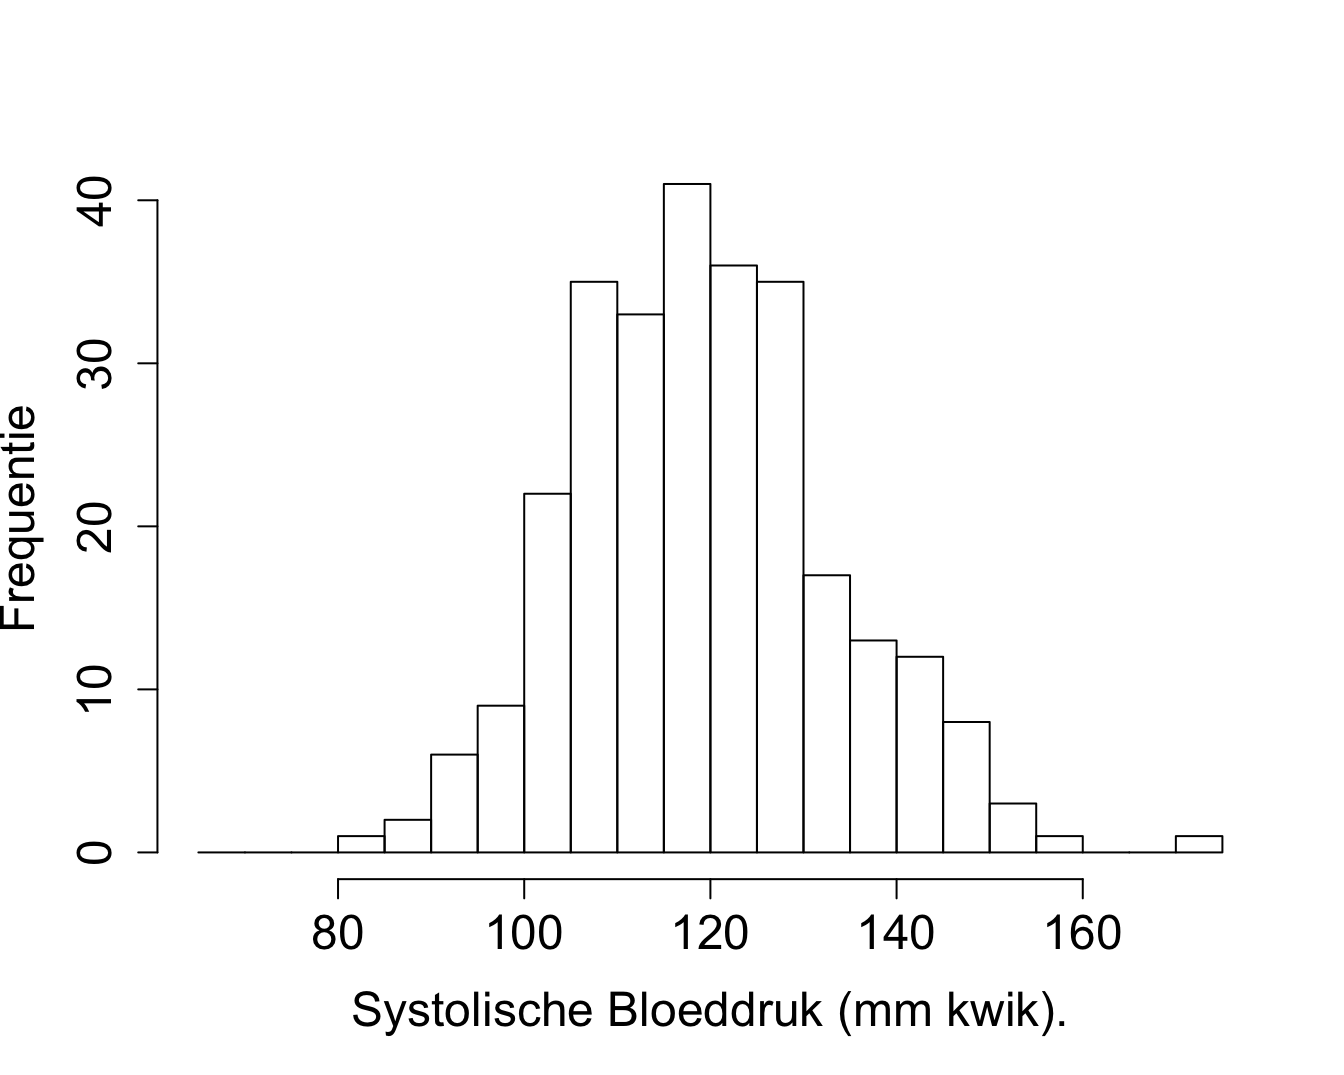
\includegraphics[width=1\linewidth]{Statistiek_2019_2020_files/figure-latex/nhanesNormalSteekproef-1} 

}

\caption{Weergave van de verdeling voor de systolische bloeddruk van gezonde personen tussen 40-65 jaar geschat aan de hand van een histogram o.b.v. de geobserveerde steekproef in de NHANES studie. (Absolute frequenties)}\label{fig:nhanesNormalSteekproef}
\end{figure}

Merk op dat de hoogte van de balken, aantallen op de y-as, weergeeft
hoeveel subjecten vallen in een bepaald interval bloeddrukken
({[}80-85{[}, {[}85-90{[}, \ldots{}). Op basis van de steekproef kunnen
we via het histogram schatten wat de kans is om een random persoon te
bemonsteren met een bloeddruk tussen 115 - 120 mm Hg uit de populatie .

\begin{Shaded}
\begin{Highlighting}[]
\NormalTok{tab <-}\StringTok{ }\KeywordTok{cbind}\NormalTok{(histAbs}\OperatorTok{$}\NormalTok{mids, histAbs}\OperatorTok{$}\NormalTok{counts)}
\NormalTok{tab}
\end{Highlighting}
\end{Shaded}

\begin{verbatim}
##        [,1] [,2]
##  [1,]  67.5    0
##  [2,]  72.5    0
##  [3,]  77.5    0
##  [4,]  82.5    1
##  [5,]  87.5    2
##  [6,]  92.5    6
##  [7,]  97.5    9
##  [8,] 102.5   22
##  [9,] 107.5   35
## [10,] 112.5   33
## [11,] 117.5   41
## [12,] 122.5   36
## [13,] 127.5   35
## [14,] 132.5   17
## [15,] 137.5   13
## [16,] 142.5   12
## [17,] 147.5    8
## [18,] 152.5    3
## [19,] 157.5    1
## [20,] 162.5    0
## [21,] 167.5    0
## [22,] 172.5    1
\end{verbatim}

\begin{Shaded}
\begin{Highlighting}[]
\NormalTok{tab[tab[, }\DecValTok{1}\NormalTok{] }\OperatorTok{==}\StringTok{ }\FloatTok{117.5}\NormalTok{, }\DecValTok{2}\NormalTok{]}\OperatorTok{/}\KeywordTok{sum}\NormalTok{(tab[, }\DecValTok{2}\NormalTok{])}
\end{Highlighting}
\end{Shaded}

\begin{verbatim}
## [1] 0.1490909
\end{verbatim}

Op basis van de steekproef wordt die kans geschat op 14.9\%.

Een histogram kan ook weergegeven worden a.d.h.v. relatieve
frequenties/densiteiten.

\begin{Shaded}
\begin{Highlighting}[]
\KeywordTok{hist}\NormalTok{(nhanesSubHealthy}\OperatorTok{$}\NormalTok{bpSys, }\DataTypeTok{xlab =} \StringTok{"Systolische Bloeddruk (mm kwik)."}\NormalTok{, }
    \DataTypeTok{breaks =} \KeywordTok{seq}\NormalTok{(}\DecValTok{65}\NormalTok{, }\DecValTok{175}\NormalTok{, }\DecValTok{5}\NormalTok{), }\DataTypeTok{freq =} \OtherTok{FALSE}\NormalTok{, }\DataTypeTok{ylab =} \StringTok{"Densiteit"}\NormalTok{, }
    \DataTypeTok{cex.main =} \FloatTok{1.5}\NormalTok{, }\DataTypeTok{cex.axis =} \FloatTok{1.5}\NormalTok{, }\DataTypeTok{cex.lab =} \FloatTok{1.5}\NormalTok{, }
    \DataTypeTok{main =} \StringTok{""}\NormalTok{)}
\end{Highlighting}
\end{Shaded}

\begin{figure}

{\centering 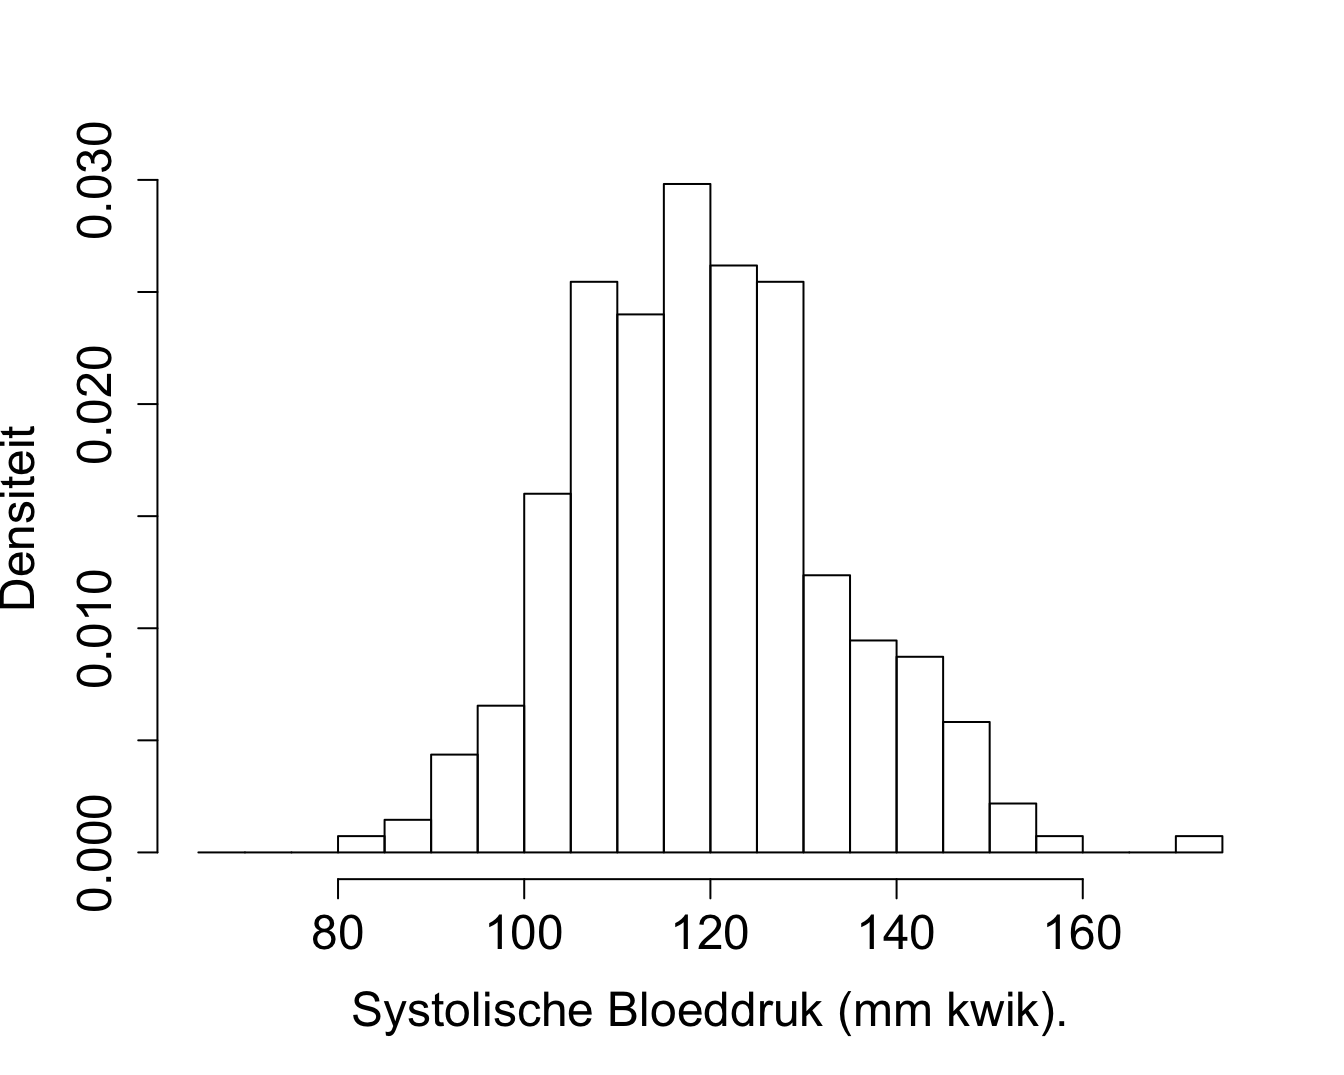
\includegraphics[width=1\linewidth]{Statistiek_2019_2020_files/figure-latex/nhanesNormalSteekproefRel-1} 

}

\caption{Weergave van de verdeling voor de systolische bloeddruk van gezonde personen tussen 40-65 jaar geschat aan de hand van een histogram o.b.v. de geobserveerde steekproef in de NHANES studie. (Relatieve frequenties)}\label{fig:nhanesNormalSteekproefRel}
\end{figure}

De oppervlakte in elke balk komt dan overeen met een kans: hoogte van de
balk x breedte van de balk. In de histogrammen hebben we voor de breedte
van de balk 5 mm Hg gekozen.

\begin{Shaded}
\begin{Highlighting}[]
\NormalTok{tab2 <-}\StringTok{ }\KeywordTok{cbind}\NormalTok{(histAbs}\OperatorTok{$}\NormalTok{mids, histAbs}\OperatorTok{$}\NormalTok{density)}
\NormalTok{tab2}
\end{Highlighting}
\end{Shaded}

\begin{verbatim}
##        [,1]         [,2]
##  [1,]  67.5 0.0000000000
##  [2,]  72.5 0.0000000000
##  [3,]  77.5 0.0000000000
##  [4,]  82.5 0.0007272727
##  [5,]  87.5 0.0014545455
##  [6,]  92.5 0.0043636364
##  [7,]  97.5 0.0065454545
##  [8,] 102.5 0.0160000000
##  [9,] 107.5 0.0254545455
## [10,] 112.5 0.0240000000
## [11,] 117.5 0.0298181818
## [12,] 122.5 0.0261818182
## [13,] 127.5 0.0254545455
## [14,] 132.5 0.0123636364
## [15,] 137.5 0.0094545455
## [16,] 142.5 0.0087272727
## [17,] 147.5 0.0058181818
## [18,] 152.5 0.0021818182
## [19,] 157.5 0.0007272727
## [20,] 162.5 0.0000000000
## [21,] 167.5 0.0000000000
## [22,] 172.5 0.0007272727
\end{verbatim}

\begin{Shaded}
\begin{Highlighting}[]
\NormalTok{tab2[tab2[, }\DecValTok{1}\NormalTok{] }\OperatorTok{==}\StringTok{ }\FloatTok{117.5}\NormalTok{, }\DecValTok{2}\NormalTok{]}
\end{Highlighting}
\end{Shaded}

\begin{verbatim}
## [1] 0.02981818
\end{verbatim}

\begin{Shaded}
\begin{Highlighting}[]
\NormalTok{tab2[tab2[, }\DecValTok{1}\NormalTok{] }\OperatorTok{==}\StringTok{ }\FloatTok{117.5}\NormalTok{, }\DecValTok{2}\NormalTok{] }\OperatorTok{*}\StringTok{ }\DecValTok{5}
\end{Highlighting}
\end{Shaded}

\begin{verbatim}
## [1] 0.1490909
\end{verbatim}

We bekomen opnieuw een schatting van 14.9\%. We geven dat weer in een
figuur, waarbij we de functie \texttt{rect()} gebruiken om de
rechthoekige balk te tekenen. A.d.h.v. de functie \texttt{text()} kunnen
we ook tekst toevoegen aan de figuur.

\begin{Shaded}
\begin{Highlighting}[]
\KeywordTok{hist}\NormalTok{(nhanesSubHealthy}\OperatorTok{$}\NormalTok{bpSys, }\DataTypeTok{xlab =} \StringTok{"Systolische Bloeddruk (mm kwik)."}\NormalTok{, }
    \DataTypeTok{breaks =} \KeywordTok{seq}\NormalTok{(}\DecValTok{65}\NormalTok{, }\DecValTok{175}\NormalTok{, }\DecValTok{5}\NormalTok{), }\DataTypeTok{freq =} \OtherTok{FALSE}\NormalTok{, }\DataTypeTok{ylab =} \StringTok{"Densiteit"}\NormalTok{, }
    \DataTypeTok{cex.main =} \FloatTok{1.5}\NormalTok{, }\DataTypeTok{cex.axis =} \FloatTok{1.5}\NormalTok{, }\DataTypeTok{cex.lab =} \FloatTok{1.5}\NormalTok{, }
    \DataTypeTok{main =} \StringTok{""}\NormalTok{)}
\KeywordTok{rect}\NormalTok{(}\DecValTok{115}\NormalTok{, }\DecValTok{0}\NormalTok{, }\DecValTok{120}\NormalTok{, tab2[tab2[, }\DecValTok{1}\NormalTok{] }\OperatorTok{==}\StringTok{ }\FloatTok{117.5}\NormalTok{, }\DecValTok{2}\NormalTok{], }\DataTypeTok{col =} \DecValTok{2}\NormalTok{)}
\KeywordTok{text}\NormalTok{(}\DecValTok{120}\NormalTok{, tab2[tab2[, }\DecValTok{1}\NormalTok{] }\OperatorTok{==}\StringTok{ }\FloatTok{117.5}\NormalTok{, }\DecValTok{2}\NormalTok{], }\KeywordTok{paste0}\NormalTok{(}\StringTok{"P(115 < X < 120) = "}\NormalTok{, }
    \KeywordTok{round}\NormalTok{(tab2[tab2[, }\DecValTok{1}\NormalTok{] }\OperatorTok{==}\StringTok{ }\FloatTok{117.5}\NormalTok{, }\DecValTok{2}\NormalTok{] }\OperatorTok{*}\StringTok{ }\DecValTok{5} \OperatorTok{*}\StringTok{ }\DecValTok{100}\NormalTok{, }\DecValTok{1}\NormalTok{), }
    \StringTok{"%"}\NormalTok{), }\DataTypeTok{col =} \DecValTok{2}\NormalTok{, }\DataTypeTok{cex =} \DecValTok{1}\NormalTok{, }\DataTypeTok{pos =} \DecValTok{4}\NormalTok{)}
\end{Highlighting}
\end{Shaded}

\begin{figure}

{\centering 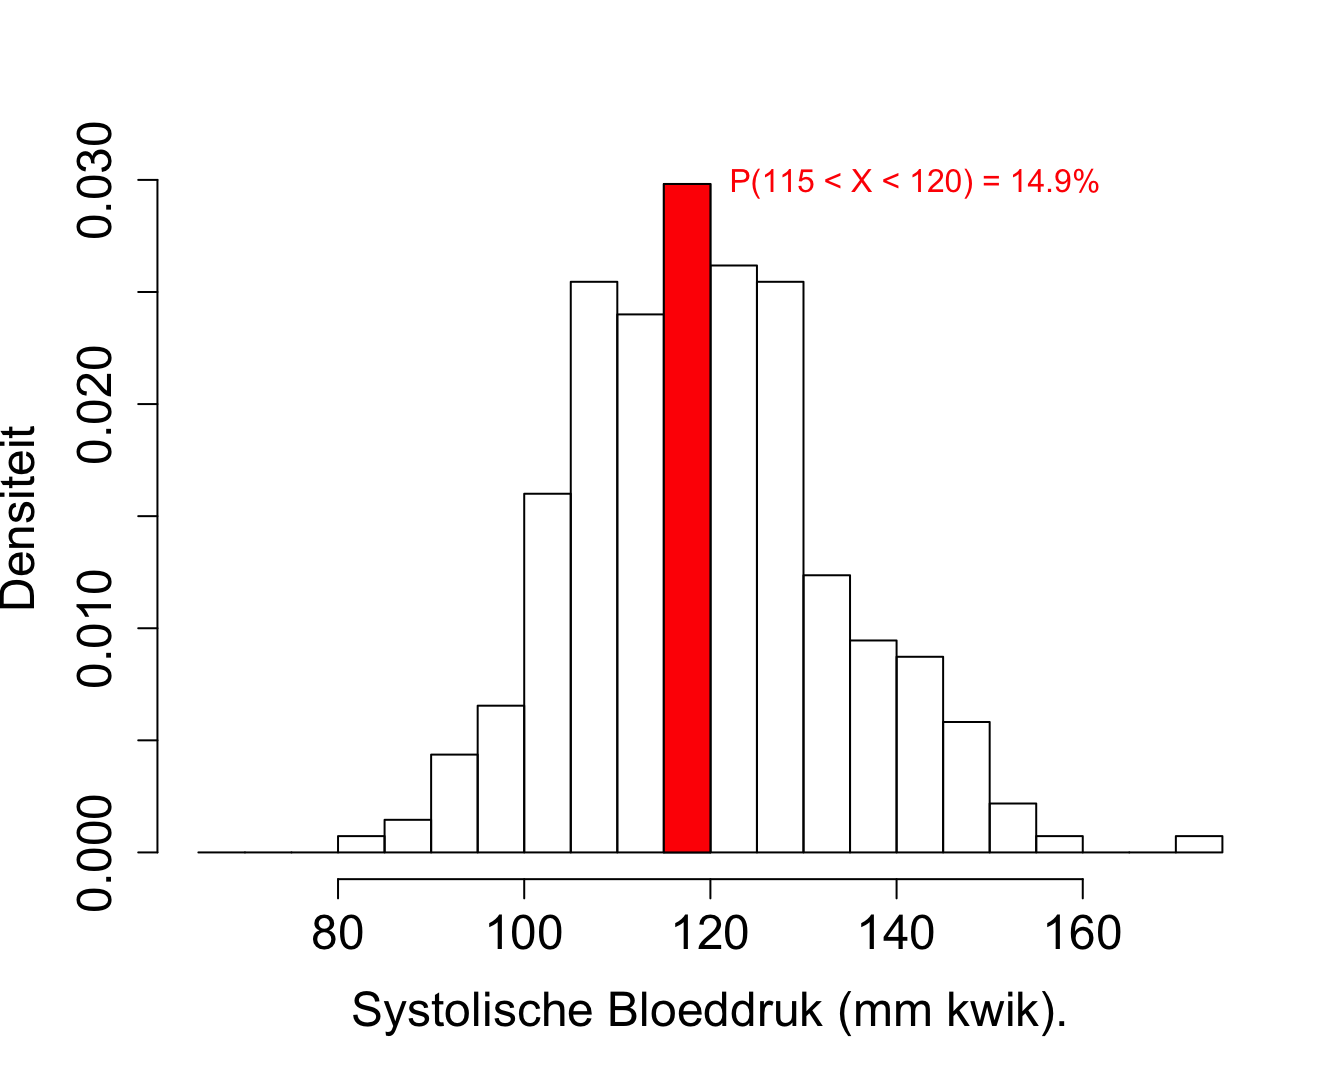
\includegraphics[width=1\linewidth]{Statistiek_2019_2020_files/figure-latex/nhanesNormalSteekproefRelProb-1} 

}

\caption{Weergave van de verdeling voor de systolische bloeddruk van gezonde personen tussen 40-65 jaar geschat aan de hand van een histogram o.b.v. de geobserveerde steekproef in de NHANES studie. (Het histogram wordt weergegeven a.d.h.v. relatieve frequenties en de geschatte kans op een bloeddruk tussen 115-120 wordt aangeduid in het rood)}\label{fig:nhanesNormalSteekproefRelProb}
\end{figure}

Als we de som van de oppervlakte van alle balken zouden berekenen is die
uiteraard gelijk aan 1. De kans om een random persoon uit de steekproef
aan te treffen tussen de laagste en hoogste waarde in de steekproef
dient immers gelijk te zijn aan 1 of 100\%!

Het histogram geeft verder weer dat de verdeling inderdaad vrij
symmetrisch blijkt te zijn en een klokvorm lijkt te hebben. Als we
kunnen veronderstellen dat de gegevens normaal verdeeld zijn dan kunnen
we de verdeling in de populatie ook schatten door enkel het gemiddelde
\(\mu\) en de variantie \(\sigma^2\) te \emph{schatten} en de
parameterschattingen in te pluggen in de Normale verdeling.

\begin{Shaded}
\begin{Highlighting}[]
\KeywordTok{hist}\NormalTok{(nhanesSubHealthy}\OperatorTok{$}\NormalTok{bpSys, }\DataTypeTok{xlab =} \StringTok{"Systolische Bloeddruk (mm kwik)."}\NormalTok{, }
    \DataTypeTok{breaks =} \KeywordTok{seq}\NormalTok{(}\DecValTok{65}\NormalTok{, }\DecValTok{175}\NormalTok{, }\DecValTok{5}\NormalTok{), }\DataTypeTok{freq =} \OtherTok{FALSE}\NormalTok{, }\DataTypeTok{ylab =} \StringTok{"Densiteit"}\NormalTok{, }
    \DataTypeTok{cex.main =} \FloatTok{1.5}\NormalTok{, }\DataTypeTok{cex.axis =} \FloatTok{1.5}\NormalTok{, }\DataTypeTok{cex.lab =} \FloatTok{1.5}\NormalTok{, }
    \DataTypeTok{main =} \StringTok{""}\NormalTok{)}
\KeywordTok{lines}\NormalTok{(grid, }\KeywordTok{dnorm}\NormalTok{(grid, }\DataTypeTok{mean =} \KeywordTok{mean}\NormalTok{(nhanesSubHealthy}\OperatorTok{$}\NormalTok{bpSys), }
    \DataTypeTok{sd =} \KeywordTok{sd}\NormalTok{(nhanesSubHealthy}\OperatorTok{$}\NormalTok{bpSys)), }\DataTypeTok{xlab =} \StringTok{"Systolische Bloeddruk (mm kwik)"}\NormalTok{, }
    \DataTypeTok{ylab =} \StringTok{"Densiteit"}\NormalTok{, }\DataTypeTok{type =} \StringTok{"l"}\NormalTok{, }\DataTypeTok{lwd =} \DecValTok{2}\NormalTok{)}
\end{Highlighting}
\end{Shaded}

\begin{figure}

{\centering 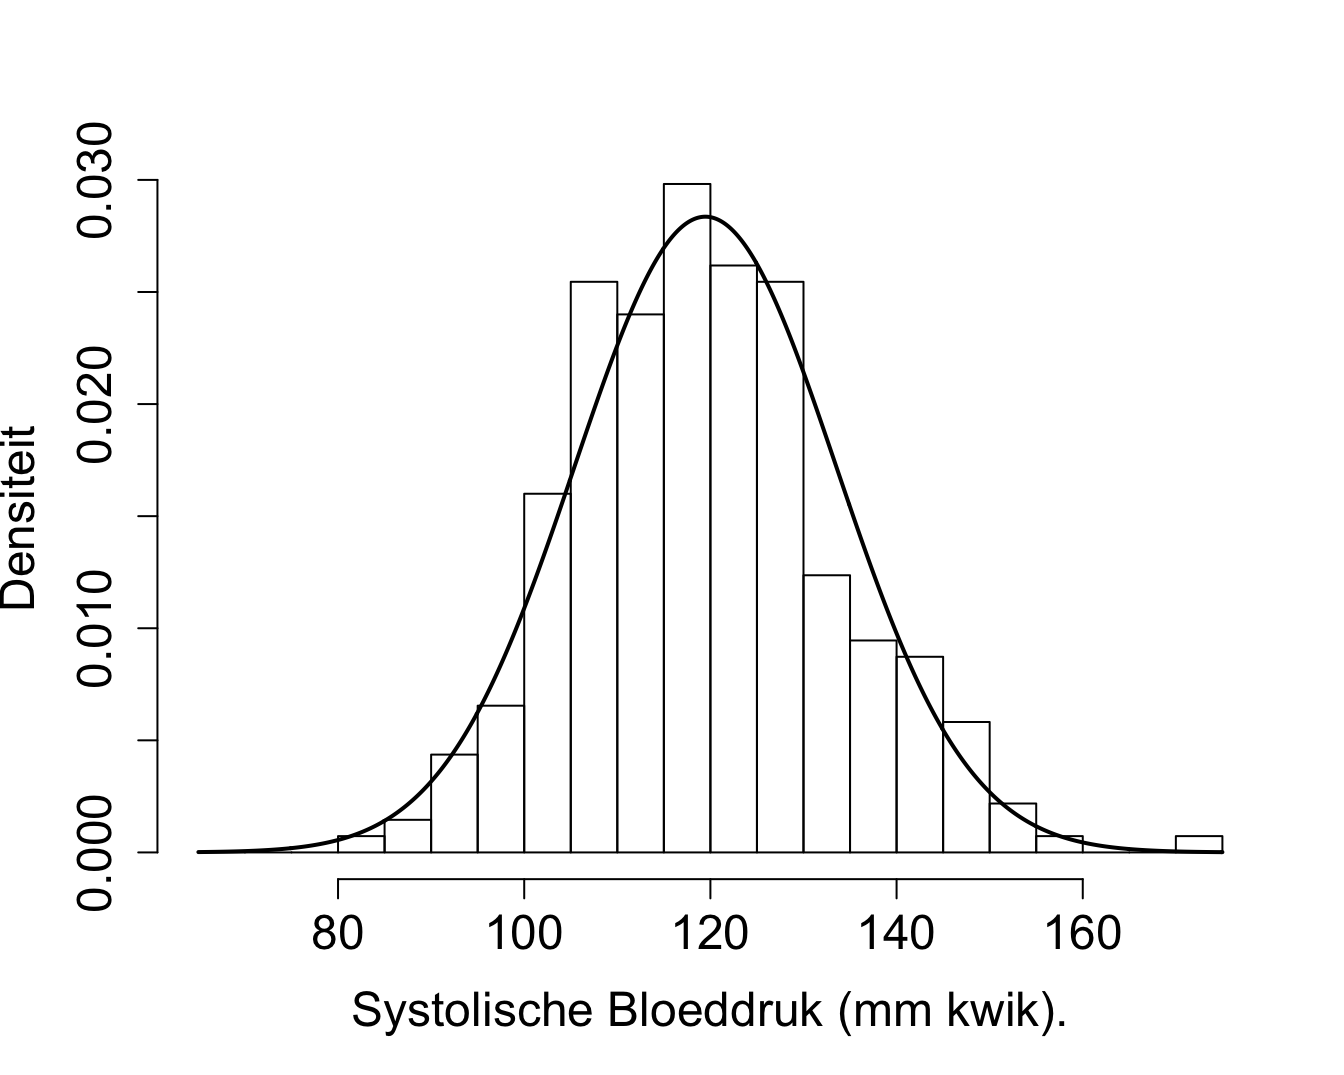
\includegraphics[width=1\linewidth]{Statistiek_2019_2020_files/figure-latex/nhanesNormalSteekproefEstimate-1} 

}

\caption{Weergave van de verdeling voor de systolische bloeddruk van gezonde personen tussen 40-65 jaar geschat aan de hand van een histogram o.b.v. de geobserveerde steekproef in de NHANES studie en a.d.h.v. een normale verdeling met geschat gemiddelde 120.4 mm Hg en geschatte variantie 129.8 (zwarte volle lijn)}\label{fig:nhanesNormalSteekproefEstimate}
\end{figure}

In plaats van kansen te berekenen door gebruik te maken van het
histogram, bestaat een alternatieve methode erin om het gemiddelde en de
variantie te schatten op basis van de steekproef. Vervolgens wordt dan
de kans berekend a.d.h.v. een normale verdeling waarbij we als
gemiddelde en variantie de overeenkomstige schattingen in de steekproef
gebruiken.

We illustreren dit in R. De normale verdeling in R wordt
geparameteriseerd a.d.h.v. het gemiddelde \(\mu\) en de standaard
afwijking \(\sigma\). Deze laatste kan direct worden geschat a.d.h.v. de
steekproef door gebruik te maken van de steekproef standaard deviatie
(functie \texttt{sd()}). De kans die we dan bekomen is

\begin{Shaded}
\begin{Highlighting}[]
\NormalTok{xBar <-}\StringTok{ }\KeywordTok{mean}\NormalTok{(nhanesSubHealthy}\OperatorTok{$}\NormalTok{bpSys)}
\NormalTok{sBar <-}\StringTok{ }\KeywordTok{sd}\NormalTok{(nhanesSubHealthy}\OperatorTok{$}\NormalTok{bpSys)}
\KeywordTok{pnorm}\NormalTok{(}\DecValTok{120}\NormalTok{, }\DataTypeTok{mean =}\NormalTok{ xBar, }\DataTypeTok{sd =}\NormalTok{ sBar) }\OperatorTok{-}\StringTok{ }\KeywordTok{pnorm}\NormalTok{(}\DecValTok{115}\NormalTok{, }\DataTypeTok{mean =}\NormalTok{ xBar, }
    \DataTypeTok{sd =}\NormalTok{ sBar)}
\end{Highlighting}
\end{Shaded}

\begin{verbatim}
## [1] 0.1397006
\end{verbatim}

Merk op dat deze schatting veel dichter ligt bij de werkelijke kans in
de populatie dan de schatting die we bekwamen d.m.v. het histogram. De
schatting o.b.v. de normale verdeling is inderdaad nauwkeuriger: we
kunnen immers gebruik maken van alle data om deze kans te schatten
gezien we het steekproefgemiddelde en de steekproefstandaarddeviatie
hebben geschat o.b.v. alle gegevens in de steekproef. Voor de kans
berekend o.b.v. het histogram konden we daarentegen enkel de gegevens
gebruiken van de personen uit de steekproef met een bloeddruk tussen 115
en 120 mmHg.\\
Uiteraard zal het in de praktijk steeds heel belangrijk zijn om na te
gaan of er voldaan is aan de aannames die we maken over de verdeling.
Anders zijn onze schattingen immers incorrect en niet bruikbaar. Het
nagaan van veronderstellingen over de verdeling is één van de
doelstellingen van data exploratie.

We kunnen nu op basis van de steekproef en de aannames van normaliteit
een grenswaarde voor de bloeddruk afleiden die extreem is voor
``gezonde'' personen in de populatie. Dat laat ons bijvoorbeeld toe om
een bloeddruk te bepalen die maar met een kans van 5\% wordt
overschreden in de populatie van gezonde subjecten:
\[P(X > t_\text{drempel}) = 5\%\] of
\[P(X \leq t_\text{drempel}) = 95\%\]

Dat kan met de functie \texttt{qnorm()} in R.

\begin{Shaded}
\begin{Highlighting}[]
\KeywordTok{qnorm}\NormalTok{(}\FloatTok{0.95}\NormalTok{, }\DataTypeTok{mean =}\NormalTok{ xBar, }\DataTypeTok{sd =}\NormalTok{ sBar)}
\end{Highlighting}
\end{Shaded}

\begin{verbatim}
## [1] 142.6011
\end{verbatim}

Deze waarde ligt dicht bij 140 mmg Hg, een grenswaarde voor hypertensie
die vaak in de literatuur wordt gebruikt.

\section{Statistieken}\label{statistieken}

Formules die gebruikt worden om parameters van de verdeling in de
populatie te schatten op basis van de steekproef, alsook het numerieke
resultaat dat men bekomt door deze formules te evalueren, worden
\emph{statistieken} genoemd. Bijvoorbeeld het rekenkundig gemiddelde van
alle systolische bloeddrukwaarden voor de verschillende subjecten in de
steekproef, is een statistiek. Statistieken zijn dus wat de onderzoekers
observeren of kunnen berekenen o.b.v. de gegevens in de steekproef;
parameters zijn wat ze eigenlijk willen weten. Omdat statistieken
berekend worden op basis van de gegevens uit de steekproef, zullen ze
variëren van steekproef tot steekproef. We zullen ze daarom noteren met
een hoofdletter (bvb. \(\bar X\) voor het steekproefgemiddelde), tenzij
we verwijzen naar de numerieke waarde die gerealiseerd wordt in een
bepaalde steekproef, in welk geval we een kleine letter gebruiken (bvb.
\(\bar x\) voor het steekproefgemiddelde).

\textbf{Belangrijke Conventie:} In de cursus gebruiken we de conventie
om \textbf{populatieparameters die een vaste waarden aannemen maar die
meestal ongekend zijn} voor te stellen door \textbf{Griekse symbolen}.
\textbf{Statistieken} waarmee we deze ongekende parameters schatten
o.b.v. een steekproef zullen we weergeven door \textbf{letters}.

Voor de normaal verdeling hebben we dus:

\begin{longtable}[]{@{}cc@{}}
\toprule
Populatie & Steekproef\tabularnewline
\midrule
\endhead
\(\mu\) & \(\bar X\)\tabularnewline
\(\sigma^2\) & \(S^2\)\tabularnewline
\bottomrule
\end{longtable}

Om hetgeen we in de steekproef observeren te kunnen veralgemenen naar de
populatie, zullen we gebruik moeten maken van methodes uit de
statistische besluitvorming wat in latere hoofdstukken aan bod komt.

De cursus is als volgt georganiseerd: In hoofdstuk \ref{chap:design}
verdiepen we ons in studiedesign. Vervolgens gaan we in op
data-exploratie in hoofdstuk \ref{chap:describe}, hierbij zullen we de
gegevens in een steekproef grondig exploreren zodoende inzicht te
verwerven in de data en hoe we ze statistisch kunnen modelleren. In
hoofdstuk \ref{chap:besluit} introduceren we de grondslagen van
statistische besluitvorming die het ons mogelijk maakt om effecten die
we observeren in de steekproef te kunnen veralgemenen naar de populatie
toe. In hoofdstukken \ref{chap:linReg}-\ref{chap:glm} zullen we meer
geavanceerde statistische modellen en methoden introduceren om data te
modelleren en voor statistische besluitvorming.

\chapter{Studiedesign}\label{chap:design}

\section{Inleiding}\label{inleiding-1}

Centraal in wetenschappelijk onderzoek is de wens en noodzaak om
theorie-gebaseerde kennis empirisch (d.w.z. door middel van observatie)
te verifiëren en op te bouwen. Terwijl theorie-gebaseerde kennis
voortvloeit uit hypothesen omtrent het bestudeerde biologische of
chemische proces, ontstaat empirische kennis door lukraak subjecten
(mensen, planten, dieren) uit een doelpopulatie te trekken volgens een
gestructureerd schema en hen vervolgens te observeren. Dit
gestructureerde schema, dat ondermeer vastlegt welke en hoeveel
subjecten in de studie worden opgenomen en eventueel wie welke
experimentele interventie zal ondergaan, noemt men het \emph{design} van
de studie of de \emph{proefopzet}. Met een goed design kunnen
betrouwbare conclusies worden getrokken op basis van de gegevens. Het
bepaalt immers welke informatie wel en niet in de dataset vervat zal
zijn. Fouten bij het design van een studie kunnen soms gecorrigeerd
worden door de statistische analyse, maar zijn helaas vaak
onherroepelijk. Het design is daarom van cruciaal belang voor een studie
en vereist evenveel aandacht als de uiteindelijke statistische analyse
van de observaties. Ook in deze cursus vormen de concepten in dit
hoofdstuk rond design wellicht het meest belangrijke onderwerp, hoewel
we er slechts beknopt op in kunnen gaan. De ideeën lijken eenvoudig,
maar dat is vaak een bedrieglijke indruk!

\begin{figure}

{\centering 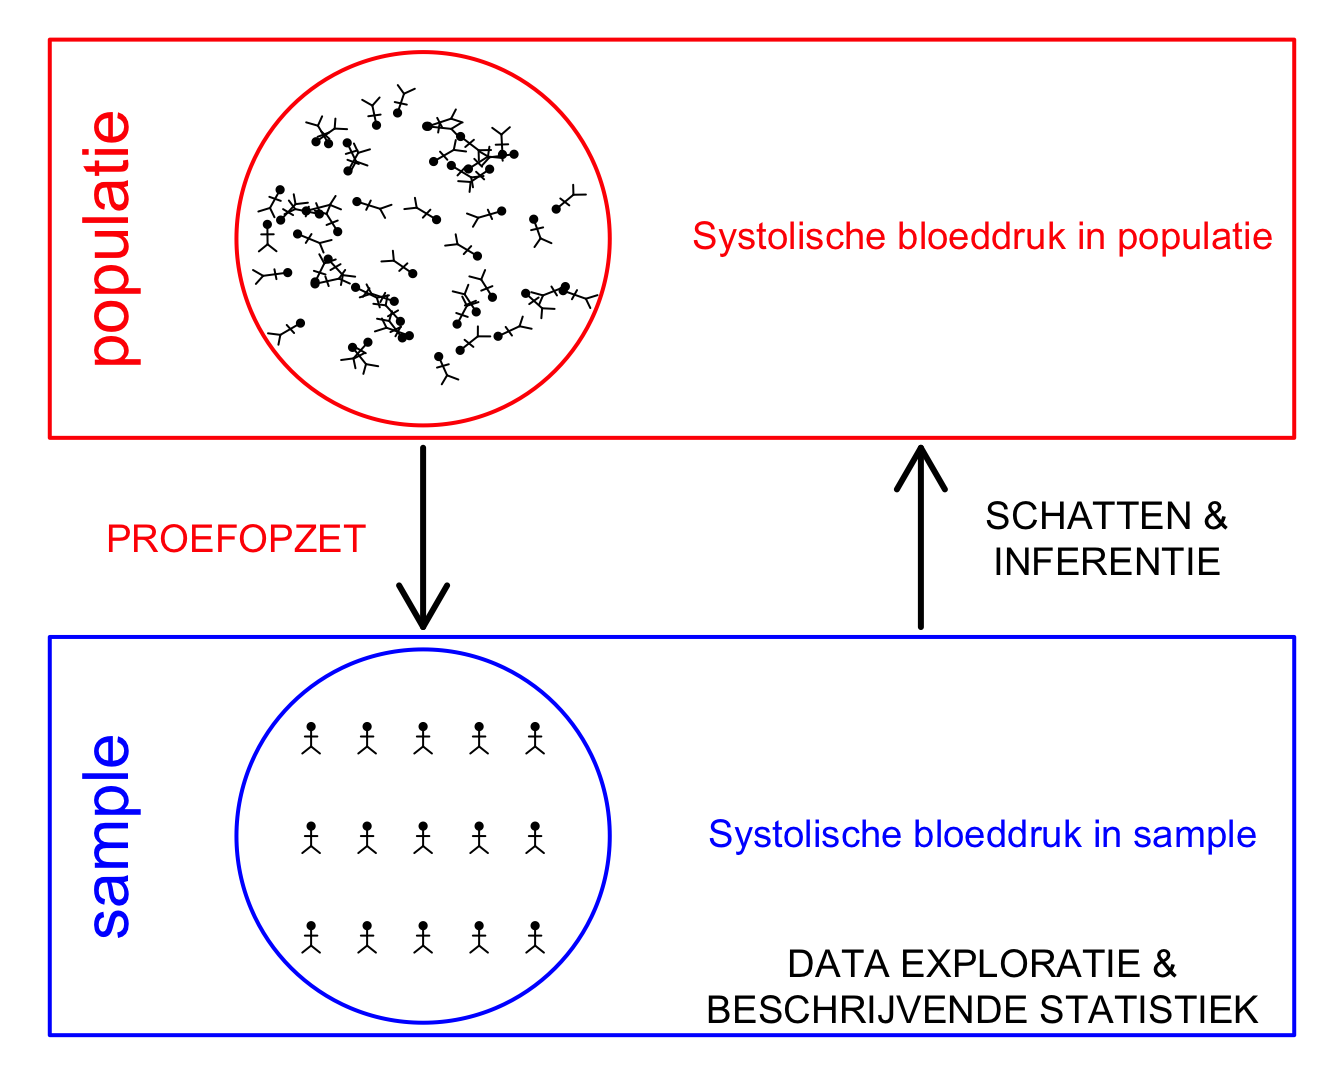
\includegraphics[width=1\linewidth]{Statistiek_2019_2020_files/figure-latex/pop2Samp2PopDesign-1} 

}

\caption{Verschillende stappen in een studie. In dit hoofdstuk ligt de focus op proefopzet.}\label{fig:pop2Samp2PopDesign}
\end{figure}

\section{Steekproefdesigns}\label{sec:steekproefdesigns}

In de praktijk vestigt men de interesse van een onderzoek op een
bepaalde biologische \emph{populatie}. Vervolgens zal men een geschikt
type en grootte van monsters of stalen (of meer algemeen experimentele
eenheden en/of subjecten genoemd doorheen deze cursus) definiëren
waarvoor men metingen zal verzamelen. Bijvoorbeeld, indien men de
grootte van de populatie salamanders van de species Plethodon jordani
wenst te bestuderen, kan men de aandacht van het onderzoek vestigen op
de bestaande populatie P. jordani in de Great Smoky Mountains (d.i. de
populatie) en vervolgens het aantal salamanders tellen op
oppervlakte-eenheden van 10 m\(^2\) (die eenheden zijn de stalen of
``experimentele eenheden''; voor elke experimentele eenheid bekomt men
aldus een meting). Indien men de impact van roofvissen op
zeebodemhabitats wenst te evalueren, dan kan het onderzoek de aandacht
vestigen op de zeebodem binnen een afstand van 500 m voor de Belgische
Noordzeekust (d.i. de biologische populatie) en kunnen vervolgens
metingen worden verzameld op stukjes zeebodem met een straal van 1 m
(d.i. de ``stalen'' in de studie). Omdat het in de praktijk bijna nooit
mogelijk is om de hele populatie te onderzoeken (alle salamanders in de
Great Smoky Mountains, de ganse zeebodem binnen een afstand van 500 m
voor de Belgische Noordzeekust), zal men zich beperken tot gegevens voor
een zogenaamde \emph{steekproef}, een beperkte verzameling stalen,
experimentele eenheden of subjecten uit de populatie.

Welke subjecten uit de populatie men precies zal bestuderen, zal
uiteraard zijn weerslag hebben op de resultaten van de uiteindelijke
analyse van de gegevens. Opdat de resultaten die men observeert voor de
steekproef veralgemeenbaar zouden zijn naar de ganse studiepopulatie, is
het noodzakelijk dat men de subjecten uit de steekproef zodanig kiest
dat ze representatief zijn voor de populatie. De basismethode om dat te
realiseren, heet \emph{eenvoudige lukrake steekproeftrekking} (in het
Engels: \emph{simple random sampling}). Ze bestaat erin te garanderen
dat elk subject in de populatie een zelfde kans heeft om in de
steekproef terecht te komen. Zo kan men bijvoorbeeld elke muis in een
kooi een nummer geven en vervolgens lukraak een aantal \(n\) van die
nummers trekken. In de praktijk, en in het bijzonder in de veldbiologie,
is die methode echter vaak moeilijk toe te passen omdat de subjecten in
de populatie bijvoorbeeld geen goed onderscheiden habitats vormen, niet
op voorhand genummerd kunnen worden of omdat de populatie een te groot
gebied bestrijkt. Zo is het bijvoorbeeld niet makkelijk om een
eenvoudige lukrake steekproef van salamanders in de Great Smoky
Mountains te bekomen omdat het bestudeerde gebied zeer groot is en de
salamanders uiteraard niet genummerd kunnen worden. In die gevallen gaan
biologen vaak over op \emph{haphazard sampling}, waarbij men op een
minder formele manier stalen verzamelt, maar er toch voor probeert te
zorgen dat de resultaten niet vertekend worden doordat bepaalde
subjecten meer kans hebben om in de steekproef terecht te komen.
Bijvoorbeeld kan men een computer lukraak plaatsen laten aanduiden in de
Great Smoky Mountains en kan men vervolgens metingen proberen te
verzamelen voor de eerste salamander die telkens in de buurt van de
aangeduide plaatsen voorbijkomt.

Sommige steekproefdesigns houden expliciet rekening met heterogeniteit
in de populatie waaruit een steekproef wordt genomen. Bij
\emph{gestratificeerde lukrake steekproeven} (in het Engels:
\emph{stratified random samples}) wordt de populatie opgedeeld in
verschillende strata, die goed onderscheiden subgroepen in de populatie
identificeren, en worden vervolgens eenvoudige lukrake steekproeven uit
elk stratum genomen. Stel bijvoorbeeld dat men karakteristieken van
stenen in een rivier wenst te beschrijven en dat stenen in verschillende
habitats voorkomen (rotsige, ondiepe waters, diepe waters, stille
binnenwaters,\ldots{}), dan kan het zinvol zijn om een gestratificeerde
lukrake steekproef te nemen om ervoor te zorgen dat er binnen elk
stratum (d.i. elke habitat) een voldoende aantal stenen verzameld
worden.

Bij \emph{geclusterde steekproeftrekking} (in het Engels: \emph{cluster
sampling}) worden clusters van meer verwante subjecten uit de populatie
getrokken. Stel bijvoorbeeld dat we de impact van verschillende vormen
van beschadiging aan bladeren van een boom wensen te meten, dan kunnen
we in een eerste fase een eenvoudige lukrake steekproef van bomen
bepalen. Vervolgens kunnen we in een tweede fase binnen elke boom een
eenvoudige lukrake steekproef van bladeren bepalen en de verschillende
gekozen bladeren aan verschillende vormen van beschadiging onderwerpen.
Dit noemt men (two stage) cluster sampling omdat bladeren afkomstig van
een zelfde boom meer verwant en bijgevolg geclusterd zijn. We zullen
later zien dat men in de analyse van gegevens uit dergelijke studie met
die clustering rekening moet houden.

Tenslotte steunt men in de biologische wetenschappen ook vaak op
\emph{systematische steekproeven} waarbij men bijvoorbeeld monsters
neemt die op vaste afstand van elkaar bekomen worden of op voorafgekozen
tijdstippen, en om die reden niet volledig lukraak genoemd kunnen
worden. Dit wordt vaak gebruikt wanneer men een omgevings- of
tijdsgradiënt wenst te beschrijven voor een bepaald proces, zoals de
wijziging in rijkdom aan species naarmate men zich verwijdert van een
vervuilingsbron. Dergelijke designs zijn nuttig en logistiek zeer
praktisch, maar kunnen vertekende resultaten opleveren wanneer de
monsters op specifieke plaatsen genomen worden die samenvallen met een
ongekende omgevings- of tijdsgradiënt (d.i. indien de gekozen plaatsen
selectief zijn en afwijkend van de globale omgevings- of tijdsgradiënt).

\subsection{Replicatie}\label{replicatie}

Replicatie betekent dat herhaaldelijke observaties worden bekomen, op
verschillende plaatsen, voor verschillende dieren of planten, op
verschillende tijdstippen, \ldots{} Dergelijke herhalingen zijn
essentieel in empirisch onderzoek omdat biologische en ecologische
systemen vaak zeer variabel zijn en de beschikbaarheid van meerdere
observaties toelaat om ruis op de gegevens te drukken. Hoewel biologen,
biotechnologen en biochemici zich goed bewust zijn van de nood voor
replicatie wordt vaak misbegrepen op welke schaal die herhalingen moeten
bekomen worden. Wellicht is er geen enkel aspect van studiedesign dat
meer verwarring veroorzaakt bij wetenschappers dan dit. Stel
bijvoorbeeld dat men een studie wenst op te zetten om het effect van
bosbranden op de rijkdom aan ongewervelde dieren te onderzoeken. Meestal
zal men dan gebruik maken van natuurlijke bosbranden. Stel dat 1
verbrand gebied gelocaliseerd wordt en vergeleken wordt met een naburig
gebied waar geen bosbrand plaatsvond. Stel verder dat men binnen elk
gebied verschillende stalen bodemkorst neemt om de rijkdom aan
ongewervelden te bepalen. Dan beschikt men wel over herhaaldelijke
metingen (namelijk verschillende stukken bodemkorst per gebied), maar
niet op de juiste schaal. De metingen voor de rijkdom aan species die
men uit het verbrande gebied bekomen heeft, meten immers de impact van
dezelfde brand. Als gevolg daarvan kan men op basis van eventuele
verschillen in species rijkdom tussen beide gebieden niet bepalen of ze
het gevolg zijn van de brand dan wel van andere verschillen tussen beide
gebieden die eveneens een impact op ongewervelden hebben. Uit dergelijke
vergelijking kan men hoogstens besluiten dat de gebieden al dan niet
verschillen, maar niet waardoor ze verschillen.

De herhaalde stukken bodemkorst in bovenstaand voorbeeld stellen
substeekproeven voor. Deze stellen geen herhalingen voor van de
bestudeerde interventie (bosbranden) en worden daarom pseudoreplicaties
genoemd. Pseudoreplicaties zijn nuttig omdat ze replicaties zijn (op een
zeker niveau) en daardoor toelaten om een deel van de ruis op de
gegevens weg te middelen. In sommige studies zijn echte replicaties
onmogelijk en is het bijgevolg onvermijdelijk om zijn toevlucht tot
pseudoreplicaties te nemen. Bijvoorbeeld, indien men een experiment
uitvoert dat kamers van constante temperatuur vereist, dan kan het best
zijn dat er binnen een gegeven instituut slechts een tweetal dergelijke
kamers beschikbaar zijn omwille van hun hoge kost. Indien men
bijvoorbeeld de impact wenst te onderzoeken van rioollozing op de
biomassa van phytoplankton in een bepaalde kuststreek, dan is er vaak
maar 1 riool waarin men echt geïnteresseerd is, terwijl het aantal
naburige lokaties zonder riool zeer uitgebreid kan zijn. In dat geval
zal men vaak stalen nemen op meerdere plaatsen zonder riool om in ieder
geval de variatie tussen controlesites (d.i. sites zonder rioollozing)
te minimaliseren. \emph{Before-After-Control-Impact (BACI) designs}
proberen verder informatie te winnen door zowel metingen te nemen vóór
de interventie (bvb. het plaatsen van een riool) als na de interventie.

\section{Experimentele studies}\label{experimentele-studies}

Studiedesigns worden opgesplits in \emph{experimentele studies of
experimenten} waar de onderzoeker eerst het biologische systeem
manipuleert en vervolgens observeert, en \emph{observationele studies}
waar de onderzoeker enkel observeert zonder zelf in het systeem in te
grijpen. In deze sectie gaan we dieper in op het eerste type studies.
Observationele studies worden besproken in Sectie
\ref{sec:observational}.

\BeginKnitrBlock{definition}[experiment]
\protect\hypertarget{def:unnamed-chunk-10}{}{\label{def:unnamed-chunk-10}
\iffalse (experiment) \fi{} }Een \textbf{experiment} is een reeks
observaties die gemaakt worden onder condities die gecontroleerd worden
door de onderzoeker. De onderzoeker controleert hierbij verschillende
factoren (zoals de keuze van de interventie voor een locatie, plant,
dier), met als doel een zuiver antwoord op de gestelde onderzoeksvraag
te bepalen. \footnote{Met ``zuiver'' wordt hier bedoeld dat de het
  zuivere interventie-effect uit de gegevens kan gehaald worden zonder
  dat het antwoord wordt beïnvloed door andere aspecten/variabelen. Dit
  wordt meer concreet in Hoofdstuk \{chap:sample\} uitgelegd. Voorlopig
  volstaat de intuïtieve betekenis van het woord.}
\EndKnitrBlock{definition}

Bijvoorbeeld, wanneer een dierenfysioloog 2 behandelingen wenst te
vergelijken tussen experimentele dieren, dan kan hij - zoals we in dit
hoofdstuk zullen zien - vermijden dat het behandelingseffect
vertekend\footnote{Voorlopig verstaan we onder het feit dat een
  schatting voor het behandelingseffect `vertekend' is, dat het foutief
  werd ingeschat of, m.a.w., dat het geschatte effect niet correct het
  zuivere effect van de behandeling weerspiegelt. Een meer concrete
  definitie volgt eveneens in Hoofdstuk \{chap:sample\}.} is door
vergelijkbare groepen dieren te creëren; bijvoorbeeld, door lukraak
(bijvoorbeeld door het opgooien van een muntstuk) te bepalen welke
behandeling aan welk dier wordt toegediend.

\subsection{De Salk Vaccin Veldstudie}\label{de-salk-vaccin-veldstudie}

Om de basisprincipes van experimentele designs in te voeren, gebruiken
we als rode draad de Salk Vaccin Veldstudie. Vooraleer dieper op deze
studie in te gaan, schetsen we de historische context.

De eerste polio-epidemie in de Verenigde Staten brak uit in 1916 en
kostte aan honderdduizenden mensen, vooral kinderen, het leven. Tegen de
jaren 1950 waren er verschillende vaccins ontwikkeld. Vooral het vaccin
dat door John Salk werd ontwikkeld, leek veelbelovend omdat het zich
veilig en effectief had getoond in laboratoriumstudies. In 1954 werd
door de National Foundation for Infantile Paralysis (NFIP) een grote
studie opgezet om de effectiviteit van het vaccin buiten het
laboratorium na te gaan. Meer concreet wenstte men na te gaan wat de
invloed was van vaccinatie op de polio-incidentie.

\BeginKnitrBlock{definition}[incidentie en prevalentie]
\protect\hypertarget{def:unnamed-chunk-11}{}{\label{def:unnamed-chunk-11}
\iffalse (incidentie en prevalentie) \fi{} }De \textbf{incidentie} van
een bepaalde ziekte of aandoening (bvb. polio) wordt gedefinieerd als
het verwachte aantal nieuwe gevallen van die ziekte dat optreedt
gedurende een vooraf bepaald tijdsinterval, uitgedrukt per eenheid van
een ziektevrije populatie. Het drukt m.a.w. de kans uit dat een individu
zonder de bestudeerde aandoening tijdens het gegeven tijdsinterval deze
aandoening zal opdoen.

De \textbf{prevalentie} van een bepaalde ziekte wordt gedefinieerd als
de proportie individuen met de ziekte in een bepaalde populatie op een
bepaald punt in de tijd.

\textbf{Einde definitie}
\EndKnitrBlock{definition}

Stel dat de NFIP het vaccin gewoon had toegediend aan een groot aantal
kinderen en dat ze een daling observeerden in de incidentie van polio
van 1953 naar 1954. Dit betekent dat de kans dat een lukraak polio-vrij
kind een polio-infectie opdeed in de loop van 1954 (d.i. de incidentie
van polio in 1954), lager is dan de kans dat lukraak polio-vrij kind een
polio-infectie opdoet in de loop van 1953 (d.i. de incidentie van polio
in 1953). In dat geval kan men niet zomaar besluiten dat het vaccin
effectief is. Immers, afgezien van de introductie van een vaccin,
varieert de incidentie van polio van jaar tot jaar. Zo zou men, indien
het vaccin niet effectief was, toch een daling in polio-incidentie van
1953 naar 1954 kunnen vaststellen in geval 1954 geen epidemisch jaar zou
zijn.

De enige manier om te ontdekken of het vaccin effectief is, is om
\emph{gelijktijdig} de incidentie van polio in 1954 te vergelijken
tussen een groep gevaccineerde kinderen (doorgaans \emph{cases} genoemd)
en een groep niet-gevaccineerde kinderen (doorgaans \emph{controles}
genoemd). Dit is wat de NFIP heeft gedaan. De deelnemers aan de studie
waren kinderen uit de leeftijdsgroepen die het meest vatbaar waren voor
polio. De studie verliep in verschillende schooldistricten in de
Verenigde Staten waar het risico op polio hoog was. Aan ongeveer 350000
kinderen uit de tweede graad werd vaccinatie voorgeschreven. Voor 125000
van hen weigerden de ouders toestemming te geven om deze vaccinatie te
laten doorgaan, zodat de groep cases uiteindelijk uit de overige 225000
kinderen bestond. Ongeveer 750000 kinderen uit de eerste en derde graad
werden vrijwillig niet gevaccineerd; zij vormden de controles.

Het feit dat de groep cases en de groep controles een verschillende
grootte hebben is niet problematisch zolang men niet het absolute
aantal, maar het percentage polio-besmettingen tussen beide groepen
vergelijkt. Toch hoeft een geobserveerd verschil in incidentie tussen
gevaccineerde en niet-gevaccineerde kinderen nog steeds niet
noodzakelijk te impliceren dat het vaccin effectief is. Hier zijn
verschillende redenen voor:

\begin{enumerate}
\def\labelenumi{\arabic{enumi}.}
\tightlist
\item
  Ten eerste zou het kunnen dat men door toeval een verschil in
  incidentie waarneemt tussen beide groepen, doordat er per toeval
  bijvoorbeeld relatief gezien minder kinderen in de gevaccineerde groep
  polio ontwikkelen. In Hoofdstuk \ref{chap:besluit} zullen we methoden
  aanleren om uit te maken of een geobserveerd vaccinatie-effect (d.w.z.
  een vaccinatie-effect dat geschat of berekend werd o.b.v. de gegevens)
  al dan niet toevallig is.
\item
  Ten tweede zou het kunnen dat kinderen uit de tweede graad sowieso
  meer vatbaar zijn voor polio en er, afgezien van het werkelijke
  vaccin-effect, voor de cases dus een hogere incidentie wordt verwacht.
\item
  Ten derde is het zo dat vooral ouders uit hoge-inkomens gezinnen
  geneigd waren om de toestemming te geven hun kind te laten vaccineren,
  zodat de groep cases hoofdzakelijk bestaat uit kinderen van
  hoge-inkomens gezinnen. Deze kinderen zijn meer vatbaar voor polio
  omdat ze, wegens de betere hygiënische omstandigheden in deze
  gezinnen, minder antilichamen tegen polio ontwikkeld hebben.
\end{enumerate}

Het geobserveerde verschil in incidentie tussen gevaccineerde en
niet-gevaccineerde kinderen weerspiegelt daarom niet alleen de
effectiviteit van het vaccin, maar ook het feit dat kinderen uit graad 2
mogelijks niet vergelijkbaar zijn met de resterende kinderen en het feit
dat cases, omwille van betere hygiënische omstandigheden, meer vatbaar
zijn voor polio dan controles. In het bijzonder is het om die reden
mogelijk om, zelfs als het vaccin effectief is, een gelijke incidentie
voor cases en controles vast te stellen. In dat geval verwart men het
effect van het vaccin met het feit dat cases meer vatbaar zijn voor
polio dan controles.

De statistische les die we hier algemeen uit kunnen trekken, is dat de
verschillende interventiegroepen zo vergelijkbaar mogelijk moeten zijn
bij de bepaling van het effect van een interventie, opdat elk verschil
in respons tussen de groepen volledig kan toegeschreven worden aan de
verschillende interventie. Wanneer de groepen cases en controles niet
volledig vergelijkbaar zijn in een bepaalde factor (zoals de vatbaarheid
voor polio, maar niet de interventie zelf), dan is het mogelijk dat het
effect van die factor verward (in het Engels: \emph{confounded}) wordt
met het effect van de interventie. Men noemt die factor dan een
confounder voor het effect van de interventie. De belangrijkste
beperking op de ondubbelzinnige interpretatie van studieresultaten is
het probleem van confounding.

\BeginKnitrBlock{example}[De nood aan controle]
\protect\hypertarget{exm:unnamed-chunk-12}{}{\label{exm:unnamed-chunk-12}
\iffalse (De nood aan controle) \fi{} }
\EndKnitrBlock{example} Hairston (1980) bestudeerde de stelling dat 2
soorten salamander (P. jordani en P. glutinosus) in de Great Smoky
Mountains mekaar rivaliseren. Hij zette daartoe experimenten op waarbij
P. glutinosus verwijderd werd van bepaalde territoria. De populatie van
P. jordani begon toe te nemen in de 3 jaren die volgden op de
verwijdering van de salamanders, maar nam al even sterk toe op
controleterritoria waar P. glutinosus niet verwijderd was. Had Hairston
geen controleterritoria onderzocht, dan had hij mogelijks de toename in
de populatie van P. jordani verkeerdelijk toegeschreven aan het
verwijderen van P. glutinosus.

\texttt{**Einde\ voorbeeld**}

\BeginKnitrBlock{definition}[confounding en confounder]
\protect\hypertarget{def:unnamed-chunk-13}{}{\label{def:unnamed-chunk-13}
\iffalse (confounding en confounder) \fi{} }\textbf{Confounding} is het
probleem dat verschillen ten gevolge van verschillende experimentele
interventies niet kunnen losgekoppeld worden van andere factoren,
\textbf{confounders} genoemd, die verschillen tussen de
interventiegroepen. Een confounder manifesteert zich als een variabele
die geassocieerd is met de blootstelling of interventie (bvb.
gevaccineerd of niet) en de uitkomst (bvb. polio-geïnfecteerd of niet),
maar die door geen van beiden zelf beïnvloed wordt. Bijvoorbeeld,
vatbaarheid voor polio is geassocieerd met de keuze van de ouders om hun
kind te laten vaccineren (d.i. de blootstelling) alsook met de
infectiestatus van het kind (d.i. de uitkomst), maar wordt door geen van
beiden zelf veroorzaakt. Confounders verstoren de associatie tussen
blootstelling en uitkomst zodat de geobserveerde associatie tussen
beiden mogelijks niet het pure effect (d.i. het causale effect) van die
blootstelling op die uitkomst uitdrukt.

\textbf{Einde definitie}
\EndKnitrBlock{definition}

\BeginKnitrBlock{example}[Confounding in mariene veldexperimenten]
\protect\hypertarget{exm:unnamed-chunk-14}{}{\label{exm:unnamed-chunk-14}
\iffalse (Confounding in mariene veldexperimenten) \fi{} }
\EndKnitrBlock{example} Om het effect te onderzoeken van roofvissen op
mariene zeebodemhabitats zou men gebieden met en zonder viskooien kunnen
vergelijken. Als men vervolgens verschillen observeert tussen beide
types gebieden, dan kan dat het gevolg zijn van het verwijderen van
roofvissen (via de kooien), maar eveneens van de aanwezigheid van kooien
(bijvoorbeeld, door schaduw die de kooi afwerpt, door de afgenomen
waterstroming, \ldots{}). Het effect van roofvissen verwijderen wordt
dus mogelijks verward met het effect van kooien plaatsen. De
aanwezigheid van kooien manifesteert zich hier dus als een confounder.
Om dergelijke confounding te vermijden, kan men controlekooien met grote
gaten plaatsen waar de vis vrij in en uit kan zwemmen, maar die voor de
rest vergelijkbaar zijn met de experimentele kooien. In dat geval zijn
beide studiegebieden van kooien voorzien en zal een vergelijking van
experimentele en controlekooien duidelijk een veel meer betrouwbare
evaluatie toelaten van het effect van roofvissen. Toch blijft dergelijke
vergelijking niet gegarandeerd vrij van confounding. Bijvoorbeeld, als
het effect van kooien plaatsen er voornamelijk in bestaat om de stroming
van water (en bijgevolg sedimentatie) te beïnvloeden, dan speelt de
vraag of de stroming van water ook niet beïnvloed wordt door het feit
dat vissen, omwille van de grote gaten, makkelijker in controlekooien
zwemmen dan in experimentele kooien.

\texttt{**Einde\ voorbeeld**}

Heel wat experten in volksgezondheid zagen de problemen met het NFIP
design en suggereerden dat de controles uit dezelfde populatie moesten
gekozen worden als de cases (d.w.z. dat ze moesten vergelijkbaar zijn).
Vergelijkbaarheid van beide groepen garanderen, zou kunnen gebeuren op
basis van menselijk oordeel. Ervaring heeft niettemin aangetoond dat dit
vaak niet succesvol is omdat het zich makkelijk leent tot het bewust of
onbewust bevoordelen van de ene groep versus de andere. Het is daarom
aangewezen om \emph{randomisatieprocedures} toe te passen, waarbij de
toewijzing van mensen aan verschillende interventie-armen volledig
lukraak gebeurt. Men zegt in dat geval dat de studie
\emph{gerandomiseerd gecontroleerd}(in het Engels: \emph{randomized
controlled}) is.

\BeginKnitrBlock{definition}[gerandomiseerde studie]
\protect\hypertarget{def:unnamed-chunk-15}{}{\label{def:unnamed-chunk-15}
\iffalse (gerandomiseerde studie) \fi{} }Een \textbf{gerandomiseerd
gecontroleerde} studie is een experiment waarbij de toewijzing van
subjecten aan de verschillende interventie-armen volledig lukraak
gebeurt zodat de toewijzing van een gegeven subject onmogelijk op
voorhand voorspeld kan worden. Als gevolg hiervan zijn de verschillende
interventiegroepen (in principe\footnote{We beklemtonen dat dit \emph{in
  principe} zo is, omdat er binnen een beperkt experiment (d.w.z met een
  relatief klein aantal proefpersonen/proefdieren) uiteraard toevallige
  verschillen tussen beide groepen kunnen ontstaan; we komen hier later
  op terug.}) in alle gekende en ongekende factoren (zoals leeftijd,
lichaamsgewicht, vatbaarheid voor polio \ldots{}) vergelijkbaar zodat
geobserveerde verschillen in uitkomst tussen de verschillende groepen
(in principe) kunnen toegeschreven worden aan de interventie (d.i. het
vaccin).

\textbf{Einde definitie}
\EndKnitrBlock{definition}

Naast de NFIP studie werd voor het Salk vaccin een gerandomiseerd
gecontroleerde studie opgezet waarbij de beslissing om aan een gegeven
kind al dan niet het vaccin toe te dienen, gemaakt werd door het
opgooien van een muntstuk. De \emph{randomisatie} werd uitgevoerd onder
kinderen die van hun ouders de toestemming kregen om zich te laten
vaccineren, indien ze aan de vaccin-groep zouden toegewezen worden. Door
de randomisatie pas uit te voeren na het krijgen van de toestemming tot
vaccinatie, kon men vermijden dat er \emph{differentiële uitval} was van
kinderen in beide groepen. Met differentiële uitval wordt bedoeld dat de
reden om niet deel te nemen aan de studie verschillend is voor de
test-en controlegroep. Dit kan vooral voorkomen in klinische studies
(d.i. experimenten bij mensen) wanneer 1 van beide behandelingen (in de
test- of controle-arm) een zware heelkundige ingreep is die vooral door
ernstig zieke mensen gemeden wordt. Wanneer er na randomisatie
differentiële uitval optreedt, dan kan men niet langer vergelijkbare
groepen garanderen.

In de gerandomiseerde Salk vaccin studie werd aan kinderen in de
controle-groep een \emph{placebo} toegediend. Dat is een inerte,
inactieve behandeling; in dit geval een injectie van zout opgelost in
water. Tijdens de studie waren de kinderen \emph{blind} voor de
behandelingscode (d.i. ze wisten niet aan welke interventiegroep ze
toegewezen waren). Dit heeft tot gevolg dat hun respons op de vaccinatie
(d.i. of ze al dan niet polio ontwikkelen) het gevolg was van het al dan
niet krijgen van het vaccin, en niet van het `idee' om al dan niet
behandeld te zijn. In deze studie lijkt het misschien onwaarschijnlijk
dat het idee om gevaccineerd te zijn de kinderen zou kunnen beschermen
tegen polio, maar de rol van het onderbewustzijn is soms sterker dan
vermoed wordt. Zo heeft men in een studie van patiënten met ernstige
post-operatieve pijn vastgesteld dat de pijn bij een derde van de
patiënten spontaan verdween na inname van een volledig neutrale
substantie!

Het blinderen van de toegediende interventie laat algemeen toe om een zo
objectief mogelijk beeld van het interventie-effect te verkrijgen.
Analoog gebruiken fysiologen in dierenexperimenten injectie met een
zoutoplossing als controle i.p.v. geen injectie. Op die manier vermijden
ze dat verschillen die men observeert tussen controledieren en dieren
die een toxische substantie ingespoten krijgen, niet het gevolg zijn van
de injectieprocedure (bijvoorbeeld, van wondjes ten gevolge van de
inspuiting), maar van de ingespoten substantie zelf.

Een verdere voorzorgsmaatregel in de Salk vaccin studie was dat ook de
dokters, die moesten vaststellen of de kinderen geïnfecteerd waren,
blind waren voor de behandeling. Op die manier voorkwam men dat de arts
bewust of onbewust kennis omtrent de gekregen vaccinatie zou gebruiken
om een beslissing te nemen over de infectiestatus. Dit zou kunnen
voorvallen wanneer het resultaat van de polio-test dubieus was en de
arts (bewust of onbewust) kennis omtrent de vaccinatie-status van zijn
patiënt gebruikt om de infectie-status te bepalen. Om dezelfde reden
zijn ook dierenfysiologen idealiter blind voor de substantie die bij
elke rat ingespoten werd.

Omdat noch de arts, noch de patiënt in de Salk vaccin studie wisten
welke behandeling werd toegediend, wordt deze studie \emph{dubbel blind}
genoemd. Dubbel blinde studies vereisen dat de verschillende
interventies er hetzelfde uitzien.

\begin{table}[t]

\caption{\label{tab:nfipStudy}De NFIP studie: aantal kinderen en incidentie (uitgedrukt per
100000 kinderen per jaar).}
\centering
\begin{tabular}{lrr}
\toprule
  & Aantal & Incidentie\\
\midrule
Vaccin & 225000 & 25\\
Controle & 725000 & 54\\
Geen toestemming & 125000 & 44\\
\bottomrule
\end{tabular}
\end{table}

Tabellen \ref{tab:nfipStudy} en \ref{tab:dbrcStudy} geven de resultaten
weer die geobserveerd werden in de NFIP studie en het \emph{dubbel
blinde gerandomiseerd gecontroleerde} (in het Engels: \emph{double blind
randomized controlled}) experiment. Op basis van Tabel
\ref{tab:dbrcStudy} stellen we vast dat de incidentie daalt van 71 tot
28 gevallen per 100000 per jaar als gevolg van toediening van het
vaccin. De enige vraag die resteert is of dergelijk verschil in
incidentie gewoon door toeval kan ontstaan wanneer in werkelijkheid het
vaccin geen effect zou hebben. Een gevorderde statistische analyse heeft
aangetoond dat het bijna onmogelijk is om dergelijk verschil in
incidentie te observeren door toeval, wanneer het vaccin geen effect
heeft. We mogen dus besluiten dat het Salk vaccin effectief is.

Merk tenslotte op dat er inderdaad confounding optreedt in de NFIP
studie. Immers de polio-incidentie lijkt er veel minder te dalen dan in
de gerandomiseerde studie, namelijk van 54 naar 25 per 100000 per jaar
als gevolg van het vaccin (zie Tabel \ref{tab:nfipStudy}). De oorzaak is
dat de controlegroep in deze studie kinderen bevat die minder vatbaar
zijn voor polio dan de vaccin-groep.

\begin{table}[t]

\caption{\label{tab:dbrcStudy}De gerandomiseerd gecontroleerde studie: aantal kinderen en incidentie (uitgedrukt per
100000 kinderen per jaar).}
\centering
\begin{tabular}{lrr}
\toprule
  & Aantal & Incidentie\\
\midrule
Vaccin & 200000 & 28\\
Controle & 200000 & 71\\
Geen toestemming & 350000 & 46\\
\bottomrule
\end{tabular}
\end{table}

\subsection{Gerandomiseerd gecontroleerde
studies}\label{gerandomiseerd-gecontroleerde-studies}

Bij randomisatie heeft elk subject in de studie (bijvoorbeeld, elk kind
in de Salk vaccin studie, elke studieplaats op de zeebodem waar men een
kooi wil plaatsen) een gekende kans om elke interventie te krijgen (bvb.
bij het opgooien van een muntje heeft men 50\% kans om het vaccin te
krijgen en 50\% kans om het placebo te krijgen), maar de te ontvangen
behandeling kan niet voorspeld worden. Vreemd genoeg wordt de nood aan
randomisatie niet steeds ingezien en maakt men vaak verkeerdelijk geen
onderscheid met \emph{systematische allocatie}.

\BeginKnitrBlock{definition}[systematische allocatie]
\protect\hypertarget{def:unnamed-chunk-16}{}{\label{def:unnamed-chunk-16}
\iffalse (systematische allocatie) \fi{} }\textbf{Systematische
allocatie} of \textbf{louter toevallige allocatie} \emph{(in het Engels:
haphazard allocation)} is een toewijzingsmethode die mogelijks op een
lukraak mechanisme lijkt, maar waarbij men de toewijzing van (sommige)
subjecten op voorhand kan voorspellen.
\EndKnitrBlock{definition}

Een typisch voorbeeld van een systematische toewijzingsmethode is er één
waarbij subjecten afgewisseld toegewezen worden aan de controle- of
interventiegroep. Het feit dat men hier de toewijzing van elk subject op
voorhand kan voorspellen, kan tot gevolg hebben dat de onderzoeker de
toewijzing manipuleert. In medisch onderzoek is het in het verleden zo
meermaals gebeurd dat artsen de al te zieke patiënten die in principe
aan de controle arm zouden moeten toegewezen worden, later op bezoek
laten komen (zodat ze de testbehandeling krijgen) of niet in de studie
opnemen. Dit kan er op zijn beurt voor zorgen dat de verschillende
groepen niet langer vergelijkbaar zijn. Om systematische allocatie te
vermijden, is het van belang om een degelijke randomisatietechniek toe
te passen. In de volgende paragrafen geven we een aantal mogelijkheden
hiertoe.

Bij \emph{eenvoudige randomisatie} worden subjecten lukraak toegewezen
aan interventie A of B door het opgooien van een muntje, dobbelsteen,
\ldots{} Vaak is het efficiënter om via de computer een
randomisatielijst te genereren die het proces van het opgooien van een
muntje nabootst. Dit vermijdt tevens de mogelijkheid dat de onderzoeker
niet naar behoren zou randomiseren (door bvb. het muntje zolang op te
gooien tot de gewenste interventiecode te zien is).

Hoewel eenvoudige randomisatie aan iedereen evenveel kans geeft om
behandeling A of B te krijgen, verzekert het niet dat beide groepen
uiteindelijk even groot zullen zijn. Zelfs in relatief grote studies kan
door toeval het verschil in aantal deelnemers in elke groep relatief
groot zijn. Men kan aantonen dat, als gevolg hiervan, het
interventie-effect doorgaans minder nauwkeurig of minder precies geschat
kan worden op basis van de gegevens dan wanneer beide groepen even groot
zouden zijn. Daarmee wordt bedoeld dat wanneer men de studie meermaals
zou uitvoeren onder identieke omstandigheden, de resultaten doorgaans
meer variabel zullen zijn van studie tot studie wanneer de relatieve
grootte van beide groepen onbeperkt is, dan wanneer men telkens groepen
van gelijke grootte eist.

Om na randomisatie 2 behandelingsarmen van gelijke grootte te bekomen,
kan \emph{gebalanceerde} of \emph{beperkte randomisatie} (in het Engels:
\emph{balanced} of \emph{restricted randomisation}) worden gebruikt.
Hierbij wordt de randomisatieprocedure zó georganiseerd dat gelijke
aantallen subjecten worden toegewezen aan interventie A of B per blok
van bijvoorbeeld 4 subjecten. Eén methode om dat te doen is om enkel
sequenties te beschouwen van de vorm (1) AABB, (2) ABAB, (3) ABBA, (4)
BABA, (5) BAAB, (6) BBAA. Met behulp van een dobbelsteen of
randomisatielijst wordt lukraak een nummer van 1 tot 6 gekozen. Stel dat
het 1 is. Dan worden de 2 eerstvolgende subjecten toegewezen aan A en de
2 daarna aan B. Vervolgens wordt een nieuw lukraak nummer tussen 1 en 6
getrokken, enzovoort\ldots{}

Gebalanceerde randomisatie met blokken van grootte 1 is equivalent aan
eenvoudige randomisatie. Dergelijke blokgrootte is dus niet opportuun
wanneer men groepen van gelijke grootte wenst te bekomen. Doorgaans is
het niettemin zinvol om relatief kleine blokgroottes te beschouwen.
Bovenstaande procedure garandeert immers dat, wanneer de studie halfweg
een blok eindigt, het verschil in aantal subjecten tussen beide groepen
hoogstens de helft van de gekozen blokgrootte bedraagt. Kleine blokken
garanderen bijgevolg kleine verschillen in aantallen deelnemers per
groep.

Bij een echte randomisatie hoeven de blokken niet allen dezelfde grootte
te hebben. Door de lengte van elk blok te variëren (bijvoorbeeld door
een lukraak mechanisme) verloopt de reeks toewijzingen van subjecten aan
interventie meer lukraak en voorkomt men dat de onderzoeker de
blokgrootte ontdekt en als gevolg daarvan de interventiecode van sommige
subjecten kan voorspellen. Immers, indien de onderzoeker de blokgrootte
kent, dan kan hij net vóór het verstrijken van elk blok voorspellen wat
de interventiecode is van het laatste subject. Gebalanceerde
randomisatie voor blokken van verschillende grootte is niet veel
moeilijker dan voor blokken van gelijke grootte. Voor het vergelijken
van 2 interventies zou men bijvoorbeeld telkens eerst lukraak kunnen
kiezen uit een blokgrootte van 2, 4 of 6 en vervolgens, zoals voorheen,
lukraak een blok van die grootte kiezen.

\BeginKnitrBlock{example}[Confounding in mariene veldexperimenten, vervolg]
\protect\hypertarget{exm:unnamed-chunk-17}{}{\label{exm:unnamed-chunk-17}
\iffalse (Confounding in mariene veldexperimenten, vervolg) \fi{} }
\EndKnitrBlock{example} Beschouw opnieuw het experiment naar het effect
van roofvissen op zeebodemhabitats. Stel dat we 12 lukrake gebieden op
de zeebodem gemarkeerd hebben en vervolgens wensen te beslissen waar we
de experimentele kooien (die effectief vis vasthouden) en de
controlekooien zullen plaatsen. Dan zouden we de kooien kunnen
randomiseren door op elke plaats een muntje op te gooien en vervolgens
een experimentele kooi te plaatsen wanneer men kop gooit en een
controlekooi anders. Die procedure is erop gericht te garanderen dat
experimentele kooien op vergelijkbare plaatsen opgesteld worden als
controlekooien. Om te vermijden dat er, per toeval, meer controlekooien
dan experimentele kooien geplaatst worden, kunnen we een gebalanceerde
randomisatie uitvoeren met blokken van grootte 2. Hoe men dit kan
uitvoeren, ligt echter minder voor de hand. Eén mogelijkheid kan erin
bestaan om de verschillende gebieden willekeurig te nummeren en die
nummers lukraak dooreen te gooien teneinde een nieuwe nummering te
bekomen die gegarandeerd lukraak is. Vervolgens kan men in volgorde van
de bekomen nummering blokken van grootte 2 randomiseren om zelfde
aantallen experimentele kooien en controlekooien te bekomen.

Zelfs na deze gebalanceerde randomisatie kan het optreden dat, door
toeval, alle controlekooien dichter bij de kust belanden dan de
experimentele kooien. Dat is niet wenselijk omdat we willen vermijden
dat het effect van het verwijderen van roofvis verward wordt met het
effect van de afstand tot de kust. Een eenvoudige oplossing lijkt erin
te bestaan om de plaatsen op de zeebodem te herrandomiseren tot men een
wenselijke opdeling bekomt. Echter, ook die oplossing is niet wenselijk
omdat ze steunt om menselijk oordeel en daardoor niet langer een vorm
van randomisatie is (d.i. ze biedt niet langer de garantie op een
lukrake opstelling).

Om te vermijden dat de controlekooien door toeval relatief gezien
dichter bij de kust opgesteld worden, kunnen we de gebalanceerde
randomisatie afzonderlijk uitvoeren op de 6 plaatsen die het dichtst bij
de kust gelegen zijn en op de 6 overige plaatsen. Op die manier
garanderen we dat er zich op de 6 plaatsen die het dichtst bij de kust
liggen, 3 controlekooien en 3 experimentele kooien bevinden, en analoog
op de 6 plaatsen die het verst van de kust verwijderd zijn. Dergelijke
vorm van randomisatie wordt \emph{gestratificeerde randomisatie} genoemd
en het bijhorend design een \emph{gerandomiseerd compleet blok design}
(in het Engels: \emph{randomized complete block design}). Alternatief
kan men de 12 gebieden markeren door eerst 6 plaatsen langs de kust te
markeren en vertrekkend vanuit elk van die 6 plaatsen, telkens 2
gebieden af te bakenen op bijvoorbeeld 100 en 500 meter van de kust.
Vervolgens kan men alternerend de controlekooi en experimentele kooi op
100 meter van de kust plaatsen. Deze laatste manier van werken is
logistiek vaak makkelijker, maar is in mindere mate te verkiezen omdat
de toewijzing van de kooien niet gerandomiseerd verloopt en omdat de
gekozen gebieden mogelijks niet als een lukrake, representatieve
verzameling gebieden op de zeebodem kan gezien worden (het is met name
een systematische steekproef). Immers, het zou kunnen dat plaatsen op
een afstand van 100 en 500 meter van de kust niet representatief zijn
omwille van een ongekende periodiciteit in bepaalde
bodemkarakteristieken.

\texttt{**Einde\ voorbeeld**}

\BeginKnitrBlock{definition}[gestratificeerde randomisatie]
\protect\hypertarget{def:unnamed-chunk-18}{}{\label{def:unnamed-chunk-18}
\iffalse (gestratificeerde randomisatie) \fi{} }\textbf{Gestratificeerde
randomisatie} \emph{(in het Engels: stratified randomisation)} is een
gebalanceerde randomisatie die afzonderlijk wordt uitgevoerd per groep
subjecten met gelijkaardige prognostische factoren\footnote{Een
  \emph{prognostische factor} is een variabele die sterk geassocieerd is
  met de bestudeerde uitkomst. Bijvoorbeeld, roken is een prognostische
  factor voor longkanker omdat het risico op longkanker sterk verschilt
  tussen rokers en niet-rokers.} (bvb. afzonderlijk op plaatsen dicht
versus ver van de kust). Ze wordt gebruikt om te voorkomen dat die
prognostische factoren door toeval niet gelijk verdeeld zouden zijn over
de verschillende interventiegroepen en als gevolg daarvan, net zoals
confounders, een storende invloed zouden hebben op de associatie tussen
behandeling en respons.

\textbf{Einde definitie}
\EndKnitrBlock{definition}

\emph{Randomized complete block designs} zijn experimentele designs
waarbij men eerst de experimentele subjecten opdeelt in blokken en
vervolgens elk niveau van de interventie binnen elk blok toepast en via
randomisatie toewijst. Men kan dit realiseren d.m.v. gestratificeerde
randomisatie waarbij de stratificatie volgens blokken verloopt.
Dergelijke designs worden vaak gebruikt wanneer biologische processen
worden bestudeerd, vooral wanneer de uitkomst zó sterk varieert tussen
subjecten dat het interventie-effect moeilijk op te pikken is vantussen
de vele ruis op de gegevens. Als de gegevens veel minder variabel zijn
per blok, laat het randomiseren van de interventie per blok immers toe
om het interventie-effect per blok te evalueren met veel minder
ruis\footnote{In Hoofdstuk chap:besluit zullen we uitleggen hoe men dit
  kan realiseren via een gepaarde analyse van de gegevens}. In de
biologische wetenschappen stellen blokken vaak experimentele subjecten
voor die gelijkaardig zijn in tijd of ruimte, hoewel men ook organismen
van dezelfde leeftijd, grootte, \ldots{} kan beschouwen.

Blok designs worden in de levenswetenschappen ook vaak gebruikt om op
een efficiente manier om te gaan met de ruis die wordt veroorzaakt door
technische variabiliteit. Bij grotere experimenten is het vaak niet
mogelijk om alle experimentele eenheden bijvoorbeeld op hetzelfde moment
op te groeien in het labo, zijn meerdere celculturen nodig, zijn
meerdere sequeneringsruns nodig voor het bepalen van de genexpressie in
alle stalen, \ldots{} Fluctuaties in de labo-condities , tussen
celculturen of van sequeneringsrun tot sequeneringsrun zorgen dan voor
extra technische ruis. In een randomized complete block design zal het
experiment opgedeeld worden in meerdere blokken (vb. tijdstippen, runs,
celculturen) en zal men de behandelingen randomizeren binnen elk blok
zodat de interventie-effecten opnieuw met veel minder ruis kunnen worden
geschat.

\BeginKnitrBlock{example}[Oxidatieve stress in Arabidopsis]
\protect\hypertarget{exm:unnamed-chunk-19}{}{\label{exm:unnamed-chunk-19}
\iffalse (Oxidatieve stress in Arabidopsis) \fi{} }
\EndKnitrBlock{example} \citet{Jacques2015} onderzochten de impact van
oxidatieve stress op het proteome in \emph{Arabidopsis thaliana}.
Hierbij bestudeerden ze het proteoom (alle proteïnen) in catalase
knock-out en wild type A. thaliana planten. De planten werden gedurende
5 weken opgegroeid in een groeikamer. Vervolgens werd het proteoom
bepaald na een controle behandeling, na 1 uur hoge lichtbehandeling of
na 3 uur hoge lichtbehandeling. Het experiment werd op drie
verschillende tijdstippen herhaald. Op elk tijdstip werden 6 proteomen
geëxtraheerd: 1 proteoom voor elk combinatie van genotype x behandeling.
Bijgevolg is dit een randomized complete block design met tijdstip als
block.

\texttt{**Einde\ voorbeeld**}

\BeginKnitrBlock{example}[Effect van bladschade]
\protect\hypertarget{exm:unnamed-chunk-20}{}{\label{exm:unnamed-chunk-20}
\iffalse (Effect van bladschade) \fi{} }
\EndKnitrBlock{example} Microbe-specifieke molecules (MSM) kunnen door
het immuunsysteem van planten worden herkend en een defensieve response
induceren die ze resistent maakt tegen bepaalde ziektes.
\citet{Valdes2014} bestudeerde het effect van MSM op de genexpressie van
Soja in een RNA-seq studie\footnote{gen-expressie studie waarbij
  gen-expressie gemeten wordt met next-generation sequencing technologie}.
De planten werden opgegroeid in 12 potten. Elke pot bevatte vijf
verschillende planten. Na 3 weken werden alle bladeren geoogst per pot.
De bladeren afkomstig van elke pot werden in twee gesneden. De ene helft
werd behandeld met een controle de andere helft met MSMs en vervolgens
werd het RNA geëxtraheerd. Om voldoende RNA te bekomen werden alle
bladhelften afkomstig van dezelfde behandeling en dezelfde pot gebruikt
per extract. Het experiment is dus een gerandomiseerd complete block
design met pot als block.

\texttt{**Einde\ voorbeeld**}

Wanneer een prognostische factor (bvb. afstand tot de kust) ongelijk
verdeeld is tussen de verschillende interventiegroepen, dan kan men toch
haar eventuele storende invloed beperken door ervoor te corrigeren als
voor een confounder. Met andere woorden, het is dan aangewezen om het
interventie-effect afzonderlijk te schatten voor subjecten met dezelfde
waarde van de prognostische factor (bijvoorbeeld afzonderlijk voor
kooien op een afstand van 100 meter van de kust en voor kooien op een
afstand van 500 meter van de kust). We zullen dieper ingaan op
dergelijke correcties in Sectie \ref{sec:observational}, alsook in het
extra deel rond het algemeen lineair regressiemodel voor de studenten
Biotechnologie en Biochemie, of in vervolgcursussen Statistiek voor de
studenten Biologie.

De volgende secties belichten een aantal verschillende types
gerandomiseerd gecontroleerde experimenten.

\subsection{Parallelle designs}\label{parallelle-designs}

In een \emph{parallel design} ontvangt 1 groep de testinterventie en de
andere groep \emph{gelijktijdig} de controle interventie. Dit is het
eenvoudigste en meest gebruikte design voor gerandomiseerd
gecontroleerde studies.

\BeginKnitrBlock{example}[Kiezelwieren en zware metalen]
\protect\hypertarget{exm:unnamed-chunk-21}{}{\label{exm:unnamed-chunk-21}
\iffalse (Kiezelwieren en zware metalen) \fi{} }
\EndKnitrBlock{example}

Medley \& Clements (1998) bestudeerden de respons van kiezelwieren op
zware metalen zoals zink in rivieren in de Rocky Mountains, Colorado,
U.S.A. Ze selecteerden daartoe tussen 4 en 7 plaatsen op 6 rivieren die
zwaar vervuild waren met zware metalen. Op elke plaats registreerden ze
een aantal fysicochemische variabelen (pH, opgeloste zuurstof,
\ldots{}), de zinkconcentratie en variabelen die de kiezelwieren
beschrijven (mate van voorkomen, diversiteit, \ldots{}). De primaire
onderzoeksvraag was of de diversiteit van kiezelwieren gelijk was in 4
groepen met verschillende concentraties zink: \(<20 \mu\)g/l,
\(21-50 \mu\)g/l, \(51-200 \mu\)g/l en \(>200 \mu\)g/l.

\texttt{**Einde\ voorbeeld**}

\subsection{Cross-over designs}\label{cross-over-designs}

In een \emph{cross-over studie} ondergaan alle experimentele subjecten
sequentieel alle interventies die in de studie vergeleken worden, maar
in een lukrake volgorde. De 2 perioden - 2 behandelingen cross-over
studie is er één waarbij subjecten lukraak toegewezen worden aan 1 van 2
groepen. Subjecten in de ene groep krijgen tijdens de eerste periode
interventie A toegediend en vervolgens interventie B in de tweede
periode. Subjecten in de andere groep krijgen tijdens de eerste periode
interventie B toegediend en vervolgens interventie A tijdens de tweede
periode.

\BeginKnitrBlock{example}[Competitie tussen species lage begroeiing]
\protect\hypertarget{exm:unnamed-chunk-22}{}{\label{exm:unnamed-chunk-22}
\iffalse (Competitie tussen species lage begroeiing) \fi{} }
\EndKnitrBlock{example}

Feinsinger et al. (1991) onderzochten competitie tussen 3 soorten lage
begroeiing in Centraal Ameri- kaanse wouden. Ze voerden een experiment
uit om de effecten van 4 interventies (relatieve dichtheid van 1
species, Besleria of Palicourea, en een tweede species Cephaelia was
10:10 (A)\footnote{Dus 10\% van het gebied wordt uitgemaakt door de ene
  species, 10\% door de andere, en 80\% door nog een derde species.},
90:10 (B), 10:90 (C), 50:50 (D)) na te gaan op responsvariabelen zoals
het aantal keren dat een bloem door kolibries wordt bezocht of het
aantal zaadjes dat rijpt per bloem. Metingen werden verzameld gedurende
4 tijdsperiodes van telkens 4 tot 6 dagen. Eén van de karakteristieken
van hun design was dat elk van 4 bestudeerde planten elke interventie
onderging in 1 van de 4 studieperiodes, zij het dat de volgorde waarin
de interventies toegepast werden anders waren voor de 4 planten (zie
onderstaande tabel).

\begin{longtable}[]{@{}lllll@{}}
\toprule
Periode & Plant 1 & Plant 2 & Plant 3 & Plant 4\tabularnewline
\midrule
\endhead
1 & A & B & C & D\tabularnewline
2 & B & C & D & A\tabularnewline
3 & C & D & A & B\tabularnewline
4 & D & A & B & C\tabularnewline
\bottomrule
\end{longtable}

\texttt{**Einde\ voorbeeld**}

Het voordeel van dit design is dat elke plant nu onder elke interventie
wordt geëvalueerd en er bijgevolg meer informatie in de gegevens
aanwezig is om het interventie-effect in te schatten dan wanneer elke
plant slechts onder 1 van de interventies wordt gezien. Immers, dit
design laat gedeeltelijk toe om elk subject met zichzelf te vergelijken
teneinde iets te leren over het interventie-effect. Men kan aantonen dat
dit tot gevolg heeft dat er (doorgaans) veel minder proefsubjecten (d.i.
planten) nodig zijn dan in een parallel design om even precies\footnote{Wat
  we concreet bedoelen met het feit dat er minder proefsubjecten nodig
  zijn om het effect met een gegeven precisie in te schatten. Voorlopig
  volstaat de intuïtieve betekenis van deze zin.} het interventie-effect
te kunnen schatten. Bovendien laat dit design toe om confounding te
vermijden in situaties waar replicatie moeilijk is, zoals volgend
voorbeeld illustreert.

\BeginKnitrBlock{example}[Effect van koper op neerstrijken van larven]
\protect\hypertarget{exm:unnamed-chunk-23}{}{\label{exm:unnamed-chunk-23}
\iffalse (Effect van koper op neerstrijken van larven) \fi{} }
\EndKnitrBlock{example}

Stel dat men het effect van koper wenst te onderzoeken op het zich
neerzetten van larven van een species ongewerveld zeedier (bvb.
zeepokken). Dan zou men kunnen 2 grote aquaria opzetten, het ene
voorzien van een koperoplossing en het andere van een inerte controle
oplossing (bvb. zeewater). Stel dat men vervolgens 1000 larven aan elk
aquarium toevoegt en na verloop van tijd het aantal larven telt dat zich
vasthecht in elk aquarium, dan kan men een geobserveerd verschil tussen
beide aantallen niet zomaar toeschrijven aan de koperoplossing omdat ook
andere verschillen tussen beide aquaria (bvb. de opstelling ervan) een
invloed kunnen hebben op het aantal larven dat zich vastzet. Om dat te
vermijden, kan men het experiment in een tweede fase opnieuw uitvoeren,
idealiter gebruik makend van dezelfde larven, maar ditmaal de
koperoplossing toedienen voor het aquarium dat voorheen met zeewater
werd gevuld en vice versa.

\texttt{**Einde\ voorbeeld**}

Niettemin zijn er in sommige situaties een aantal problemen met
cross-over designs die het inschatten van het interventie-effect
compliceren. Een eerste probleem is dat het effect van de interventie in
de eerste periode een tijdje kan blijven bestaan in de tweede periode.
Men noemt dit een \emph{carry-over effect}. In dat geval wordt het
moeilijk (of zelfs onmogelijk) om de effecten van beide interventies van
elkaar te onderscheiden en los te koppelen. Om die reden zijn crossover
designs het meest aangewezen voor interventies die slechts een korte
termijn effect hebben. Ook wanneer het interventie-effect wijzigt over
de tijd is het moeilijk met dit design om correct te beschrijven hoe
goed de ene interventie werkt t.o.v. de andere. Men zegt in dat geval
dat er een \emph{interactie} is tussen de interventie en de periode
waarin ze toegediend wordt. Omdat dergelijke interacties de analyse van
de gegevens bemoeilijken en de resultaten tevens minder precies maken,
zijn cross-over designs vooral nuttig voor de studie van responsmetingen
die stabiel blijven over een lange tijd heen.

\subsection{Factoriële designs}\label{factoriele-designs}

\emph{Factoriële designs} zijn experimentele designs met als doel het
effect van meer dan 1 interventie te testen. Deze designs zijn zo
opgezet dat alle interventies in combinatie met elkaar voorkomen zodat
men interacties tussen interventies kan meten. Ze worden zeer frequent
gebruikt in de bio-wetenschappen.

\BeginKnitrBlock{definition}[interactie of effect-modificatie]
\protect\hypertarget{def:unnamed-chunk-24}{}{\label{def:unnamed-chunk-24}
\iffalse (interactie of effect-modificatie) \fi{} }Een
\textbf{interactie} tussen 2 interventies drukt uit dat een combinatie
van 2 interventies een effect heeft dat groter of kleiner is dan de som
van de effecten van de afzonderlijke interventies (op een zekere
schaal).
\EndKnitrBlock{definition}

\BeginKnitrBlock{example}[Grootte van salamanderlarven]
\protect\hypertarget{exm:unnamed-chunk-25}{}{\label{exm:unnamed-chunk-25}
\iffalse (Grootte van salamanderlarven) \fi{} }
\EndKnitrBlock{example}

Maret \& Collins (1996) bestudeerden de effecten van (ongewerveld)
voedselniveau (d.i. veel of weinig bruine garnalen) en de
aan-/afwezigheid van kikkervisjes op de grootte van salamanderlarven.
Voor elk van de 4 combinaties van voedselniveau en aan/afwezigheid van
kikkervisjes werden 8 aquaria opgezet en na verloop van tijd werd de
grootte van de snuit van salamanders in elk aquarium opgemeten. Noteer
in het bijzonder de 4 interventies als volgt: A (veel voedsel en
kikkervisjes), B (weinig voedsel en kikkervisjes), C (veel voedsel en
geen kikkervisjes), D (weinig voedsel en geen kikkervisjes). In de
afwezigheid van interacties, drukt een vergelijking van groep A-B met
C-D het effect uit van kikkervisjes. Analoog drukt een vergelijking van
groep A-C met B-D het effect uit van het voedselniveau. De aanwezigheid
van groep D laat toe om interacties te evalueren, d.i. om na te gaan of
het effect van het voedselniveau anders is alnaargelang de aanwezigheid
van kikkervisjes.

Denk voor dit voorbeeld zelf even na hoe u op basis van gegevens voor
groepen A, B, C en D zou nagaan of er een interactie is tussen
voedselniveau en de aanwezigheid van kikkervisjes.

\texttt{**Einde\ voorbeeld**}

Bovenstaand voorbeeld geeft aan dat, indien men op voorhand weet dat 2
of meerdere interventies niet interageren, factoriële designs toelaten
om de effecten van elk van de afzonderlijke interventies te evalueren
met kleinere groepen subjecten en meer precisie dan afzonderlijke
parallelle designs.

\BeginKnitrBlock{example}[Groei van esdoorn versus beuk]
\protect\hypertarget{exm:unnamed-chunk-26}{}{\label{exm:unnamed-chunk-26}
\iffalse (Groei van esdoorn versus beuk) \fi{} }
\EndKnitrBlock{example}

Poulson \& Platt (1996) bestudeerden de effecten van lichtinval (nl.,
bevindt men zich onder het bladerdak, op een plaats waar 1 boom is
omgevallen, of op een plaats waar meerdere bomen omgevallen zijn) en
hoogte van de zaailingen (1-2 m, 2-4 m of 4-8 m) op het verschil in
groei tussen zaailingen van de esdoorn en de beuk. De respons was het
verschil in groei tussen gepaarde zaailingen van elke soort. Op elk van
de 9 combinaties van lichtinval en hoogte van de zaailingen werden 5
metingen voor de respons verzameld. Hoe zou u het effect van lichtinval
op het groeiverschil tussen esdoorn en beuk evalueren? En het effect van
de grootte van de zaailingen? Wat betekent het dat er een interactie is
tussen de lichtinval en grootte van de zaailingen?

\texttt{**Einde\ voorbeeld**}

Voorwaarden om factoriële designs te gebruiken, zijn (a) dat de
verschillende interventies kunnen gecombineerd worden (en de combinatie
van interventies dus geen hoge risico's stelt voor de studiesubjecten,
d.i. iets waar men vooral bij medische interventies moet waakzaam zijn),
en (b) dat men echt geïnteresseerd is in de aanwezigheid van
interacties. Factoriële designs bestaan eveneens in complexere vormen
waar ze meer dan 2 interventies betrekken. In die gevallen, alsook
wanneer elke interventie vele niveaus heeft, kan het aantal combinaties
van factoren hoog oplopen en bijgevolg eveneens het aantal subjecten dat
in de studie moet opgenomen worden. Om dit te vermijden, kan men
overstappen op \emph{fractionele factoriële designs} waar men niet alle
combinaties van interventies probeert uit te testen.

\subsection{Quasi-experimentele
designs}\label{quasi-experimentele-designs}

Algemeen noemt men een experiment met test- en controlegroep, maar
zonder lukrake allocatie aan 1 van beide interventiegroepen, een
\emph{quasi-experimenteel design}. Het grote nadeel van dit design is
dat verschillen tussen beide groepen niet gegarandeerd kunnen
toegeschreven worden aan verschillen in behandelingswijze.

\BeginKnitrBlock{example}[Gezondheidscampagne in Wales]
\protect\hypertarget{exm:unnamed-chunk-27}{}{\label{exm:unnamed-chunk-27}
\iffalse (Gezondheidscampagne in Wales) \fi{} }
\EndKnitrBlock{example}

Om het effect van een gezondheidscampagne in Wales te evalueren, werd
een Engels controlegebied gekozen dat ver van Wales verwijderd was
(zodat het niet blootgesteld was aan de campagne) (Tudor-Smith et al.,
1998). Metingen werden verzameld in beide gebieden, zowel vóór de
campagne als 6 jaar later. Hoewel er verbetering werd opgemerkt over de
jaren heen, konden geen verschillende evoluties tussen beide groepen
aangetoond worden.

\texttt{**Einde\ voorbeeld**}

\section{Observationele studies}\label{sec:observational}

Terwijl in een gecontroleerd experiment de onderzoeker zelf beslist
welke subjecten een bepaalde interventie ondergaan, observeert men in
een \emph{observationele studie} verschillende subjecten die (mogelijks
om zelfgekozen redenen) verschillende interventies hebben ondergaan en
probeert men hier vervolgens het interventie-effect uit af te leiden.
Bijvoorbeeld, om na te gaan wat het effect is van de aanwezigheid van de
salamandersoort P. glutinosus op de groei van de populatie P. jordani
zou men in een observationele studie verschillende studiegebieden
vergelijken waar er om natuurlijke redenen al dan niet een populatie P.
glutinosus aanwezig is. Dergelijke studies zijn wel gecontroleerd (omdat
men studiegebieden met en zonder P. glutinosus vergelijkt), maar niet
experimenteel (omdat de onderzoeker niet zelf beslist in welke
studiegebieden de salamandersoort P. glutinosus aanwezig is). Inderdaad,
in een experimentele studie zou men ingrijpen door in sommige
studiegebieden de populatie P. glutinosus te verwijderen en in andere
niet.

Het grote nadeel van observationele studies is dat verschillen in
uitkomst tussen verschillende interventiegroepen niet gegarandeerd
kunnen toegeschreven worden aan de blootstelling of interventie. Dit
komt doordat deze groepen vaak in meer verschillen dan alleen hun
blootstelling. Problemen van confounding zijn dus inherent aan
observationele studies. Stel bijvoorbeeld dat men vaststelt dat de
populatie P. jordani \emph{sneller groeit} in gebieden met dan zonder P.
glutinosus. Dan kunnen we besluiten dat er een associatie of verband is
tussen de aanwezigheid van P. glutinosus en de populatiegroei van P.
jordani. Maar dat op zich bewijst niet dat het toevoegen van de
salamandersoort P. glutinosus in gebieden waar ze niet aanwezig is, een
gunstig effect zal hebben op de populatiegrootte van P. jordani (d.i.
dat het toevoegen van P. glutinosus een \emph{causaal effect} op P.
jordani heeft). Er kunnen immers verborgen confounders zijn: zo zou het
kunnen dat men meer kans heeft om P. glutinosus aan te treffen in
voedselrijke gebieden, waar de populatie P. jordani ook makkelijker zal
toenemen omwille van de aanwezigheid van voedsel (maar niet omwille van
de aanwezigheid van P. glutinosus). De rijkdom aan voedsel is in dit
geval een confounder omdat (in overeenkomst met de eerdere definitie
voor confounders) zowel de aanwezigheid van P. glutinosus als de groei
van P. jordani geassocieerd zijn met de rijkdom aan voedsel, maar geen
van beiden de rijkdom aan voedsel beïnvloeden.

Omwille van confounders is het belangrijk in observationele studies om
bij de subjecten waarvoor metingen verzameld worden, zorgvuldig
prognostische factoren voor de bestudeerde uitkomst te meten die
mogelijks ook met de blootstelling geassocieerd zijn. Voor die
confounders die gemeten zijn, kan men immers corrigeren in de
statistische analyse. Bijvoorbeeld, om de vergelijking van gebieden met
en zonder P. glutonisus te corrigeren voor de confounder voedselrijkdom,
kan men proberen een index te verzamelen voor de voedselrijkdom van elk
gebied en vervolgens de analyse afzonderlijk uitvoeren bij gebieden met
dezelfde voedselrijkdom. Men zegt dan dat de analyse of het geschatte
effect van P. glutonisus op de groei van P. jordani \emph{gecontroleerd}
(in het Engels: \emph{adjusted} of \emph{controlled}) werd voor de
voedselrijkdom van het studiegebied.

\BeginKnitrBlock{example}[Simpson's paradox]
\protect\hypertarget{exm:unnamed-chunk-28}{}{\label{exm:unnamed-chunk-28}
\iffalse (Simpson's paradox) \fi{} }
\EndKnitrBlock{example}

De Universiteit van Californië, Berkeley voerde verschillende jaren
terug een observationele studie uit om na te gaan of er
geslachtsdiscriminatie was bij de toelatingsexamens. Gedurende de
studieperiode namen 8442 jongens en 4321 meisjes deel aan het examen.
Ongeveer 44\% van de jongens en 35\% van de meisjes werd toegelaten tot
de universiteit. Ervan uit gaande dat jongens en meisjes even capabel
zijn om voor het examen te slagen (er is immers geen bewijs van het
tegendeel), krijgen we hier de indruk dat jongens en meisjes anders
behandeld worden bij de toelatingsprocedure.

Omdat de toelatingsexamens verschillend waren naargelang de
studierichting, werd bovenstaande analyse per studierichting opgesplitst
om na te gaan welke faculteiten verantwoordelijk waren voor mogelijke
discriminatie. De resultaten voor de 6 grootste richtingen staan in
Tabel \ref{tab:sexbias} getabuleerd (resultaten voor de andere
richtingen waren analoog). In alle studierichtingen ligt het
slaagpercentage hoger bij de meisjes dan bij de jongens, behalve in
richting E waar de jongens het lichtjes beter doen. Dit lijkt
paradoxaal, wetende dat het algemene slaagpercentage voor de jongens dat
van de meisjes ruim overstijgt. Hoe kunnen we dit verklaren?

De verklaring is dat de moeilijkheidsgraad van de studierichting (en
verwant hiermee de keuze van studierichting) een confounder is voor de
associatie tussen geslacht en de slaagkans. Immers, zoals blijkt uit
Tabel \ref{tab:sexbias} hebben jongens meer de neiging om
studierichtingen te kiezen waar de slaagkansen hoog zijn: meer dan 50\%
van de jongens schreven zich in voor studierichtingen A en B, waar de
slaagkansen hoger waren dan 50\%; meer dan 90\% van de meisjes
kandideerde voor de andere studierichtingen die veel zwaardere
toelatingsexamens hadden.

De vergelijking van de slaagkansen per studierichting in Tabel
\ref{tab:sexbias} levert een analyse op die gecontroleerd is voor de
keuze van studierichting. Na deze controle blijkt relatief weinig
verschil in slaagkansen tussen jongens en meisjes. De statistische les
is dat relaties tussen percentages kunnen omkeren naarmate men ze al dan
niet in subgroepen bekijkt. Dit noemt men \emph{Simpson's paradox}.

\begin{table}[t]

\caption{\label{tab:sexbias}Resultaten van de toelatingsexamens volgens geslacht en studierichting.}
\centering
\begin{tabular}{lrrrr}
\toprule
  & Jongens(aantal) & Jongens(geslaagd \%) & Meisjes(aantal) & Meisjes (geslaagd \%)\\
\midrule
A & 825 & 62 & 108 & 82\\
B & 560 & 63 & 25 & 68\\
C & 325 & 37 & 593 & 34\\
D & 417 & 33 & 375 & 35\\
E & 191 & 28 & 393 & 24\\
\addlinespace
F & 373 & 6 & 341 & 7\\
\bottomrule
\end{tabular}
\end{table}

\texttt{**Einde\ voorbeeld**}

\BeginKnitrBlock{example}[Confounders in de NHANES studie]
\protect\hypertarget{exm:unnamed-chunk-29}{}{\label{exm:unnamed-chunk-29}
\iffalse (Confounders in de NHANES studie) \fi{} }
\EndKnitrBlock{example}

De National Health and Nutrition Examination Survey (NHANES 1) is een
studie naar gezondheids- en voedingsgewoontes bij 7188 vrouwen tussen 25
en 74 jaar die opgevolgd werden van 1971 tot 1975 en van 1981 tot 1984
(Schatzkin et al., 1987). De onderzoekers vonden een positieve
associatie tussen alcoholconsumptie en borstkanker (d.w.z. een hogere
kans op borstkanker bij hogere consumptiegraad). Een grote vraag in deze
studie was of deze associatie werkelijk het gevolg was van
alcoholconsumptie of het gevolg van een mogelijks groot aantal andere
factoren die met alcohol consumptie geassocieerd zijn. Het zou
bijvoorbeeld kunnen dat vrouwen die meer alcohol verbruiken ook meer
roken en om die reden gemakkelijker borstkanker ontwikkelen. In dat
geval kan men door de storende invloed van roken mogelijks waarnemen dat
het risico op borstkanker toeneemt met stijgend alcoholverbruik, zelfs
wanneer in werkelijkheid het alcoholverbruik geen (causaal) effect heeft
op borstkanker. Roken is in dat geval een confounder omdat het hogere
risico op borstkanker voor alcoholverbruikers dan niet (alleen) het
gevolg is van hun alcoholverbruik, maar (ook of vooral) van hun
rookgedrag.

Om de invloed van roken op de associatie tussen borstkanker en
alcoholconsumptie te doen verdwijnen, heeft men de statistische analyse
uitgevoerd bij vrouwen met hetzelfde rookgedrag. Immers, door de analyse
te beperken tot vrouwen met hetzelfde rookgedrag, zijn de groepen
vrouwen die wel versus niet alcohol consumeren, beter vergelijkbaar en
is er dus niet langer een storende invloed van roken. Men zegt in dat
geval dat men in de analyse gecorrigeerd (in het Engels: adjusted) heeft
voor het rookgedrag, waarmee men bedoelt dat men het effect van alcohol
op borstkanker heeft voorgesteld voor vrouwen met hetzelfde rookgedrag.
In deze studie vond men dat er na correctie voor roken een associatie
bleef bestaan tussen alcoholverbruik en borstkanker. Men besloot dat
alcoholconsumptie een verhoogd risico op borstkanker impliceert.

\texttt{**Einde\ voorbeeld**}

Goede analyses van observationele studies controleren voor confounders.
In de praktijk is het echter zeer moeilijk om alle mogelijke confounders
te kennen voor de associatie tussen een blootstelling en een respons. En
zelfs wanneer men ze zou kennen, is het vaak onmogelijk om ze allen te
meten. Om die reden zijn de resultaten van observationele studies
doorgaans minder betrouwbaar dan de resultaten van gerandomiseerd
gecontroleerde experimenten. Niettemin zijn observationele studies
krachtig en belangrijk omdat het in vele situaties onmogelijk is om een
gerandomiseerd experiment uit te voeren. Zo is het praktisch quasi niet
mogelijk om een gerandomiseerde experiment uit te voeren naar het effect
van bosbranden op de rijkdom aan ongewervelde dieren in de grond omdat
vuur moeilijk te manipuleren valt. Hoewel de onderzoeker in bepaalde
studiegebieden brandhaarden kan aanbrengen, bestaat immers steeds het
risico dat de brand uit de hand loopt. Om die reden bestudeert men vaak
gebieden waar op natuurlijke wijze of door brandstichters brand is
ontstaan. Hoewel dergelijke studie typisch te kampen hebben met
problemen van confounding, hebben observationele studies, mits correctie
voor gemeten confounders, in het verleden heel wat nuttige en correctie
informatie gebracht, zoals de boodschap dat roken longkanker veroorzaakt
(Doll \& Hill, 1964).

\BeginKnitrBlock{example}[Observationele versus gerandomiseerde studies]
\protect\hypertarget{exm:unnamed-chunk-30}{}{\label{exm:unnamed-chunk-30}
\iffalse (Observationele versus gerandomiseerde studies) \fi{} }
\EndKnitrBlock{example}

Foetussen kunnen in de baarmoeder onderzocht worden via echografie.
Verschillende experimenten op dieren hebben aangetoond dat dergelijk
onderzoek kan leiden tot laag geboortegewicht. Om na te gaan of dat ook
zo is bij mensen werd verschillende jaren terug een observationele
studie opgezet in het Johns Hopkins ziekenhuis, Baltimore. Na correctie
voor een aantal confounders stelden de onderzoekers vast dat baby's die
via echografie onderzocht werden in de baarmoeder gemiddeld een lager
geboortegewicht hadden dan baby's die niet blootgesteld werden aan
echografie. Kunnen we hieruit besluiten dat echografie leidt tot lager
geboortegewicht?

Het antwoord is nee. We kunnen dit niet zomaar besluiten omdat de baby's
die blootgesteld waren aan echografie mogelijks niet vergelijkbaar waren
met de andere baby's in de studie. Om een duidelijk antwoord te vinden,
werd later een gerandomiseerd gecontroleerde studie uitgevoerd. Deze
toonde een matig beschermend effect van echografie aan! De reden dat de
observationele studie hier een andere conclusie opleverde, is omdat
echografie ten tijde van deze studie vooral werd toegepast bij
probleemzwangerschappen. Om die reden waren de baby's die in de
observationele studie waren blootgesteld aan echografie doorgaans a
priori minder gezond dan de andere baby's. Of het al dan niet om een
probleemzwangerschap ging, was dus een confounder voor de associatie
tussen geboortegewicht en blootstelling aan echografie.

\texttt{**Einde\ voorbeeld**}

\section{Prospectieve studies}\label{subsec:design:prosp}

In \emph{prospectieve studies} wenst men een associatie tussen een
blootstelling en uitkomst te bepalen door eerst een groep subjecten met
de blootstelling en een groep subjecten zonder de blootstelling te
identificeren en vervolgens (na zekere tijd) de gewenste uitkomst voor
elk subject te observeren. Men kiest bijvoorbeeld 10 studiegebieden met
en 10 studiegebieden zonder P. glutinosus en na 5 jaar evalueert men
voor elk studiegebied hoe groot de populatie P. jordani is.

Prospectieve studies zijn vaak \emph{longitudinaal}. Dat betekent dat ze
de evolutie van processen over de tijd heen onderzoeken door op
verschillende tijdstippen metingen voor respons (en vaak ook
blootstelling) te verzamelen. Bijvoorbeeld kan men 10 studiegebieden met
en 10 studiegebieden zonder P. glutinosus identificeren en jaarlijks
(gedurende 5 jaar) evalueren hoe groot de populatie P. jordani is.
Dergelijke prospectieve longitudinale studies laten toe om na te gaan
hoe de grootte van de populatie P. jordani evolueert over de tijd in
functie van de aanwezigheid van een andere salamandersoort. Ze worden
(prospectieve) \emph{cohort studies} genoemd. Meer algemeen zijn dit
longitudinale studies waarbij voor elke subject in de studie op
verschillende tijdstippen de uitkomst (en eventueel ook de
blootstelling) worden geregistreerd, zonder dat de subjecten
noodgedwongen eerst opgedeeld worden in een groep cases met de
blootstelling en een groep controles zonder de blootstelling.
Bijvoorbeeld kan men lukraak 20 gebieden in de studie opnemen en
gedurende 5 jaar, jaarlijks registreren hoe groot de populatie P.
jordani en hoe groot de populatie P. glutinosus is. Op basis van al die
metingen kan men vervolgens nagaan of er een associatie is tussen de
grootte van beide populaties. Merk op dat experimentele studies
noodgedwongen prospectief zijn.

\BeginKnitrBlock{example}[Vruchtbaarheid van schelpdieren]
\protect\hypertarget{exm:unnamed-chunk-31}{}{\label{exm:unnamed-chunk-31}
\iffalse (Vruchtbaarheid van schelpdieren) \fi{} }
\EndKnitrBlock{example}

Ward \& Quinn (1988) verzamelden 37 eicapsules van het schelpdier
Lepsiella Vinosa aan de litorale zone en 42 eicapsules aan de mosselzone
van een rotsige kust. De onderzoekers wensten na te gaan of er een
verschil was in het gemiddeld aantal eitjes per capsule tussen beide
zones. Deze studie is prospectief vermits de onderzoekers eerst 2 types
studiegebieden (d.i. 2 blootstellingen) identificeren en vervolgens de
uitkomst observeren.

\texttt{**Einde\ voorbeeld**}

\section{Retrospectieve studies}\label{subsec:design:retro}

In \emph{retrospectieve studies} wenst men een associatie tussen een
blootstelling en een bepaalde aandoening te bepalen door eerst een groep
subjecten met de aandoening en een groep subjecten zonder de aandoening
te identificeren en vervolgens op te sporen welke blootstelling ze in
het verleden ondervonden hebben. Men kiest bijvoorbeeld 100
longkankerpatiënten en 100 mensen zonder longkanker en vergelijkt
vervolgens het DNA-profiel tussen beiden. Dergelijke studies worden ook
\emph{case-controle studies} of \emph{case-referent studies} genoemd
omdat de groep subjecten met de aandoening doorgaans \emph{cases} worden
genoemd, en de groep subjecten zonder de aandoening \emph{controles}.
\emph{Pas echter op:} het is niet omdat men subjecten met (zonder) de
aandoening \emph{cases} (\emph{controles}) noemt in een bepaalde studie,
dat het om een case-controle studie gaat! Zo is ook de Salk vaccin
studie geen case-controle studie hoewel gevaccineerde
(niet-gevaccineerde) kinderen \emph{cases} (\emph{controles}) werden
genoemd.

\BeginKnitrBlock{example}[Genetische associatiestudies]
\protect\hypertarget{exm:brcaLeu}{}{\label{exm:brcaLeu} \iffalse (Genetische
associatiestudies) \fi{} }
\EndKnitrBlock{example}

Genetische associatiestudies zijn erop gericht om na te gaan of
polymorfismen (d.i. verschillen in DNA sequentie tussen individuen) in
bepaalde genen geassocieerd zijn met bepaalde fenotypes, bijvoorbeeld of
het polymorfisme in het BRCA1 gen geassocieerd is met borstkanker. Vaak
bestudeert men relatief zeldzame aandoeningen, in welk geval
case-controle studies zeer efficiënt zijn. Immers, door via het design
vast te leggen dat het DNA-profiel moet gemeten worden van 100
borstkankercases en 100 controles kan men met een beperkt aantal
metingen toch een voldoende aantal cases evalueren. In prospectieve
studies daarentegen zou men met een borstkankerprevalentie van 1\% al
10000 mensen moeten evalueren om een 100-tal cases te garanderen.

In dit voorbeeld beschouwen we zo'n case-controle studie die 800
borstkankercases en 572 controles omvatte. Informatie omtrent het
BRCA1-polymorfisme werd bekomen via DNA-analyse en staat getabuleerd in
Tabel \ref{tab:leu}. We stellen vast dat 89 van de 800 cases het allel
Leu/Leu bezitten, of 11.1\%, en 56 van de 572 controles, of 9.8\%. Dit
suggereert dat de aanwezigheid van het allel Leu/Leu prevalenter is bij
mensen met borstkanker. In latere hoofdstukken zullen we vaststellen dat
dergelijk verschil in prevalentie van blootstelling aan het allel
Leu/Leu voldoende klein is om door toeval te kunnen ontstaan wanneer er
in werkelijkheid geen associatie is tussen het polymorfisme in BRCA1 en
borstkanker. Er is bijgevolg onvoldoende bewijs voorhanden om te kunnen
besluiten dat er een associatie is tussen het polymorfisme in BRCA1 en
borstkanker.

Merk op dat, hoewel onder de mensen die het allel Leu/Leu bezitten
\(89/145=61.4\%\) aan bortskanker lijdt, dit cijfer niet veralgemeenbaar
is naar de ganse bevolking. Dit komt doordat het percentage
borstkankerpatiënten in deze studie vastgekozen is door het design en
dus niet het werkelijke risico op borstkanker weerspiegelt!

\begin{table}[t]

\caption{\label{tab:leu}Kruistabel van borstkanker-status versus BRCA1-allel.}
\centering
\begin{tabular}{lrrr}
\toprule
Genotype & Controles & Cases & totaal\\
\midrule
Pro/Pro & 266 & 342 & 608\\
Pro/Leu & 250 & 369 & 619\\
Leu/Leu & 56 & 89 & 145\\
Totaal & 572 & 800 & 1372\\
\bottomrule
\end{tabular}
\end{table}

\texttt{**Einde\ voorbeeld**}

Er zijn 2 mogelijke variaties van case-controle studies. In
\emph{niet-gematchte case-controle studies} is de controlegroep een
goedgekozen steekproef uit de populatie subjecten zonder de aandoening.
Het algemeen principe om controles te kiezen is hier (a) om subjecten te
kiezen die op basis van hun karakteristieken, maar afgezien van hun
uitkomst (bvb. ziektestatus), case zouden kunnen geweest zijn, en (b) om
hen onafhankelijk van de blootstelling te kiezen. In \emph{gematchte
case-controle studies} zoekt men voor elke case 1 of meerdere
controlesubjecten die vergelijkbaar zijn met de case in termen van
belangrijke prognostische variabelen voor de bestudeerde aandoening,
zoals leeftijd en geslacht. Bijvoorbeeld kan men voor elke case een
controle kiezen van exact dezelfde leeftijd en geslacht. Omdat elke case
nu beter vergelijkbaar is met zijn/haar controle verhoogt men aldus de
controle voor confounders bij het onderzoeken van het effect van de
risicofactor op de uitkomst. Matching kan echter leiden tot een groot
verlies aan observaties, met name wanneer heel wat controles verloren
gaan doordat ze niet aan de matching criteria voldoen.

Beide types case-controle design vergen elk hun eigen statistische
analyse. In deze cursus beperken we ons grotendeels tot niet-gematchte
case-controle studies. De analyse van gematchte case-controle studies is
complexer omdat deze rekening moet houden met de verwantschap tussen
cases en gematchte controles.

Het grote voordeel van case-controle studies is dat ze nuttig aangewend
kunnen worden voor de studie van zeldzame aandoeningen. Dit is zo
vermits het design toelaat om op voorhand een groep individuen met de
aandoening te selecteren en het bijgevolg niet nodig is om te wachten
tot een voldoende aantal subjecten de bestudeerde aandoening heeft
opgelopen, teneinde over voldoende informatie te beschikken om een
accurate vergelijking te maken van het risico in beide
blootstellingsgroepen. Een nadeel is dat ze retrospectief zijn en dus
beroep doen op historische data of het geheugen van de proefpersonen om
informatie te verzamelen over de blootstelling en andere factoren. Dit
kan de resultaten mogelijks vertekenen, in welk geval men van
\emph{recall bias} spreekt. Dergelijke vertekening is vooral
problematisch wanneer ze niet in even erge mate optreedt voor cases als
voor controles. Bijvoorbeeld, omdat cases aan een ziekte lijden,
herinneren ze zich vaak beter aan welke risicofactoren ze in het
verleden blootgesteld zijn. Als gevolg hiervan kan men bepaalde
blootstellingen verkeerdelijk associëren met de bestudeerde ziekte
wanneer die blootstellingen in werkelijkheid even prevalent waren voor
cases als controles, maar frequenter gerapporteerd werden door cases dan
controles. Dergelijke problemen stellen zich minder of niet in
genetische associatiestudies waar men via DNA-analyse vroegere
`blootstellingen' opspoort.

Case-controle studies zijn net als cohort studies gevoelig aan het
probleem van (ongemeten) confounders. In dat opzicht is een groot nadeel
de moeilijke keuze van een goede (d.w.z. vergelijkbare) controlegroep.

\section{Niet-gecontroleerde studies}\label{niet-gecontroleerde-studies}

In \emph{niet-gecontroleerde studies} is er geen gelijktijdige
controlegroep aanwezig en ondergaan alle subjecten (op elk tijdstip)
bijgevolg dezelfde interventie. Vermits er in dergelijke studies geen
groep subjecten is die een andere interventie ondergaan, is het
moeilijker en vaak zelfs onmogelijk om op basis van deze studies het
effect van interventies te evalueren. In deze sectie bespreken we een
aantal van deze studies.

\subsection{Pre-test/Post-test studies}\label{subsec:prepost}

Een \emph{pre-test/post-test studie} is een studie waarbij een bepaalde
karakteristiek gemeten wordt bij een groep subjecten, die vervolgens
onderworpen worden aan een zekere interventie en bij wie diezelfde
karakteristiek tenslotte opnieuw gemeten wordt. Het behandelingseffect
wordt dan vaak gemeten door de metingen na interventie te vergelijken
met de metingen vóór interventie. Stel bijvoorbeeld dat men de impact
wenst in te schatten van het plaatsen van een waterzuiveringsstation
langs een rivier op de biomassa van phytoplankton. Dan zou men op basis
van verschillende waterstalen metingen kunnen verrichten zowel vóór als
na het plaatsen van het station, en vervolgens beide groepen metingen
kunnen vergelijken.

Hoewel dergelijk design zowel metingen met als zonder interventie
levert, blijft een groot nadeel de afwezigheid van een controlegroep.
Wanneer men een wijziging in uitkomst observeert tussen de tijdstippen
van afname van de 2 metingen, kan men immers niet garanderen dat dit het
gevolg is van de interventie, vermits ook andere factoren die de
uitkomst beïnvloeden, gewijzigd kunnen zijn gedurende de studie.
Bijvoorbeeld, hoewel bovenstaande studie nuttige inzichten kan
verschaffen in de impact van waterzuiveringsstations, blijft steeds de
vraag met dit soort designs of eventuele wijzigingen in de biomassa van
phytoplankton toe te schrijven zijn aan het zuiveringsstation of eerder
natuurlijke evoluties weerspiegelen ten gevolge van de gewijzigde
weersomstandigheden, etc\ldots{}

\subsection{Cross-sectionele surveys}\label{cross-sectionele-surveys}

\emph{Cross-sectionele surveys} onderzoeken een groep subjecten op een
bepaald punt in de tijd afgezien van hun blootstelling of uitkomst, in
tegenstelling tot cohort en case-controle studies. Bijvoorbeeld, stel
dat een ecoloog een aantal meren onderzoekt en voor elk meer de grootte
opmeet alsook de mate van divergentie in morfologische karakteristieken
tussen vissen van een bepaalde species. Dan kunnen de bekomen metingen
worden gebruikt om na te gaan of zich meer divergentie voordoet in grote
dan in kleine meren. Dit studiedesign wordt cross-sectioneel genoemd
omdat men op 1 bepaald tijdstip verschillende subjecten (d.i. meren)
onderzoekt, afgezien van blootstelling (d.i. grootte van het meer) of
uitkomst (d.i. divergentie).

De resultaten uit cross-sectionele studies kunnen moeilijk
interpreteerbaar zijn wanneer ze een tijdscomponent betrekken. Stel
bijvoorbeeld dat men in zo'n studie een negatieve associatie vaststelt
tussen leeftijd en lichaamslengte. Dan kan dit zijn omdat oudere mensen
krimpen, maar ook omdat de jongere generaties doorgaans groter worden
dan in het verleden het geval was, of omdat grote mensen sneller
sterven!

\chapter{Data exploratie en beschrijvende
statistiek}\label{chap:describe}

\section{Inleiding}\label{inleiding-2}

Om de resultaten van een experimentele of observationele studie te
rapporteren, is het uiteraard niet mogelijk om per subject waarvoor
gegegevens verzameld werden in de studie de bekomen gegevens neer te
schrijven. Met de veelheid aanwezige informatie is het integendeel
belangrijk de gegevens gericht samen te vatten en voor te stellen. Zelfs
wanneer het duidelijk is welke analyse er moet uitgevoerd worden, moet
er eerst een basisbeschrijving komen van de verzamelde gegevens. Dit zal
mee helpen aangeven of er geen fouten zijn gemaakt tijdens het onderzoek
of bij de registratie van gegevens. Eventuele anomalieën of zelfs fraude
worden in deze fase opgespoord en tenslotte krijgt men een indruk of
voldaan is aan de onderstellingen (bvb. de onderstelling dat de gegevens
Normaal verdeeld zijn \footnote{Zie Sectie \ref{sec:qq}.}) die aan de
grond liggen van de voorgestelde statistische analyses in de latere
fase.

De eerste vraag die moet gesteld worden bij het benaderen van een echte
data set is:

\begin{enumerate}
\def\labelenumi{\arabic{enumi}.}
\tightlist
\item
  Wat is de oorspronkelijke vraagstelling (geweest), waarom zijn deze
  gegevens verzameld?
\item
  Hoe en onder welke omstandigheden zijn de subjecten gekozen en de
  variabelen gemeten? Hierbij stelt men meteen de vraag naar het design
  van de studie, alsook hoeveel subjecten werden aangezocht voor
  meetwaarden en hoeveel daar uiteindelijk echt van in de database zijn
  terecht gekomen (m.a.w. of gegevens die men gepland had te verzamelen,
  om een of andere reden toch niet bekomen werden). Bovendien laat dit
  toe om te evalueren of verschillende subjecten in de studie al dan
  niet meer verwant zijn dan andere subjecten en of de analyse hier
  rekening mee moet houden.
\item
  Is er een specifieke numerieke code die een ontbrekend gegeven of
  ander type uitzondering voorstelt in plaats van een echte meetwaarde?
\end{enumerate}

Als het vertrekpunt duidelijk is en alle variabelen goed beschreven
zijn, kan men starten met een betekenisvolle exploratie van de
gerealiseerde observaties.

\begin{figure}

{\centering 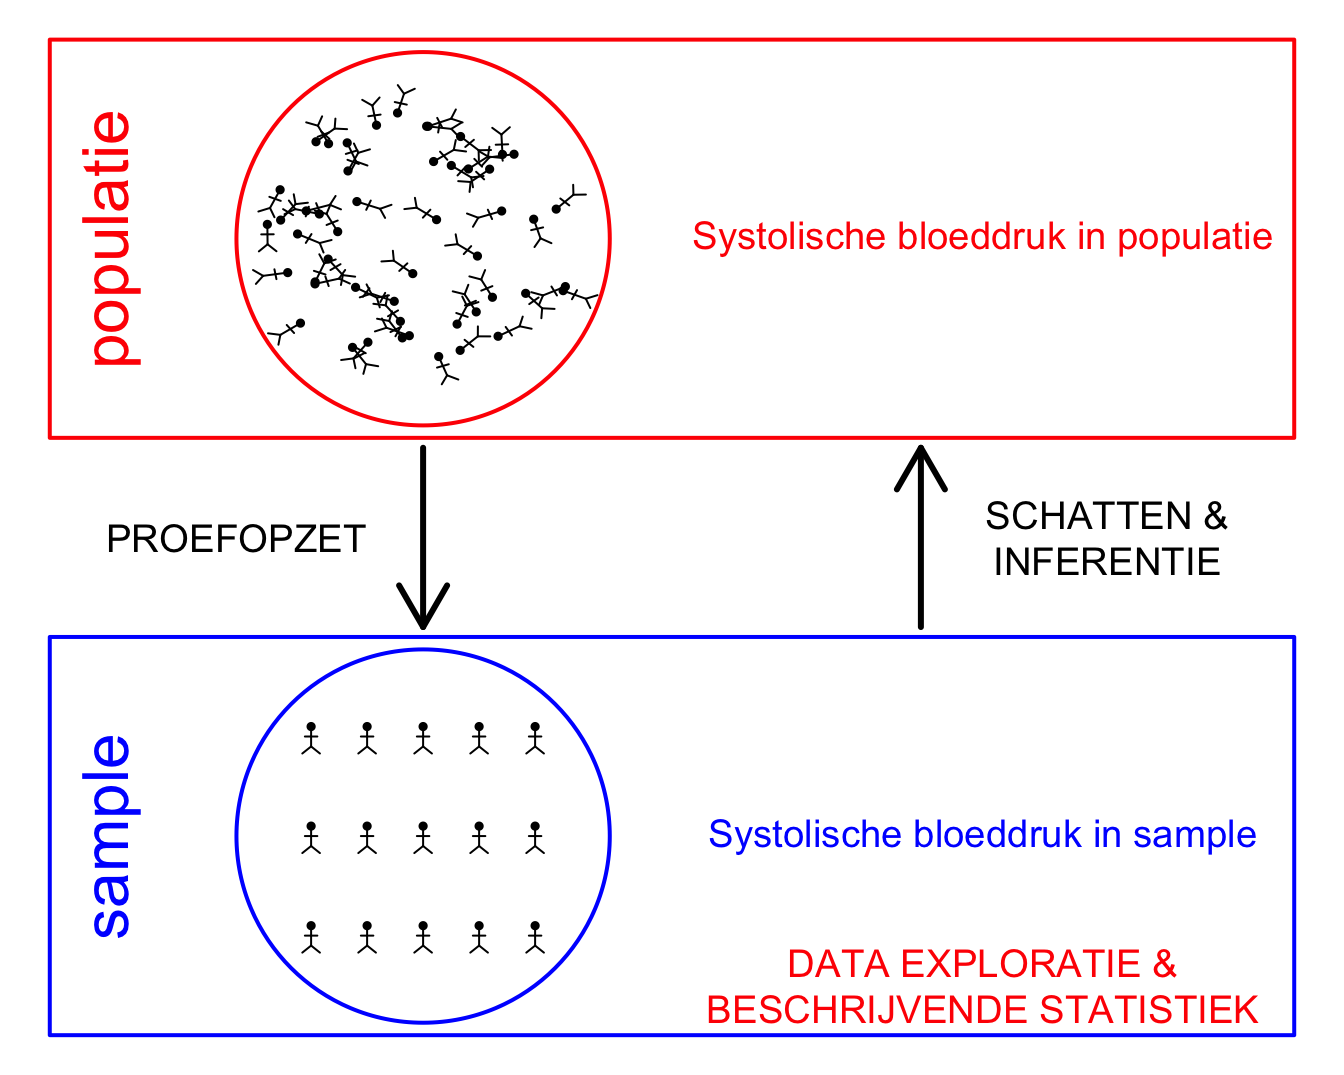
\includegraphics[width=1\linewidth]{Statistiek_2019_2020_files/figure-latex/pop2Samp2PopDataExpl-1} 

}

\caption{Verschillende stappen in een studie. In dit hoofdstuk ligt de focus op de data-exploratie en beschrijvende statistiek}\label{fig:pop2Samp2PopDataExpl}
\end{figure}

Dit hoofdstuk zullen werken rond een centrale dataset: de NHANES studie.

\BeginKnitrBlock{example}[NHANES studie]
\protect\hypertarget{exm:nhanesEx}{}{\label{exm:nhanesEx} \iffalse (NHANES
studie) \fi{} }
\EndKnitrBlock{example}

De National Health and Nutrition Examination Survey (NHANES) wordt sinds
1960 op regelmatige basis of genomen. In dit voorbeeld maken we gebruik
van de gegevens die werden verzameld tussen 2009-2012 bij 10000
Amerikanen en die werden opgenomen in het R-pakket NHANES. Er werd een
groot aantal fysische, demografische, nutritionele, levelsstijl en
gezondheidskarakteristieken gecollecteerd in deze studie (zie Tabel
\ref{tab:nhanesDatExpl}). Merk op dat ontbrekende waarnemingen hier
gecodeerd worden a.d.h.b. de code \texttt{NA} (Not Available / Missing
Value)

\texttt{**Einde\ voorbeeld**}

\begin{table}[t]

\caption{\label{tab:nhanesDatExpl}Overzicht van een aantal variabelen uit de NHANES studie.}
\centering
\begin{tabular}{rlrlrrrrrll}
\toprule
ID & Gender & Age & Race1 & Weight & Height & BMI & BPSysAve & TotChol & SmokeNow & Smoke100\\
\midrule
51624 & male & 34 & White & 87.4 & 164.7 & 32.22 & 113 & 3.49 & No & Yes\\
51625 & male & 4 & Other & 17.0 & 105.4 & 15.30 & NA & NA & NA & NA\\
51630 & female & 49 & White & 86.7 & 168.4 & 30.57 & 112 & 6.70 & Yes & Yes\\
51638 & male & 9 & White & 29.8 & 133.1 & 16.82 & 86 & 4.86 & NA & NA\\
51646 & male & 8 & White & 35.2 & 130.6 & 20.64 & 107 & 4.09 & NA & NA\\
\addlinespace
51647 & female & 45 & White & 75.7 & 166.7 & 27.24 & 118 & 5.82 & NA & No\\
\bottomrule
\end{tabular}
\end{table}

\section{Univariate beschrijving van de variabelen}\label{sec:univar}

In de regel begint men met een \emph{univariate} inspectie: elke
variabele wordt apart onderzocht. Het is absoluut aan te raden om
hierbij eerst alle ruwe gegevens te bekijken door middel van grafieken
(zie verder) alvorens naar samenvattingsmaten (zoals het gemiddelde)
over te stappen. Dit laat toe om een idee te krijgen hoe de
geobserveerde waarden van een veranderlijke verdeeld zijn in de
studiegroep (bvb. welke verdeling de bloeddrukmetingen in de studie
hebben) en of er eventuele \emph{uitschieters} (d.i. extreme metingen of
\emph{outliers}) zijn. Met outliers worden observaties aangegeven die
ten opzichte van de geobserveerde verdeling van de waarden in de data
set, extreem zijn, buitenbeentjes.

\begin{Shaded}
\begin{Highlighting}[]
\CommentTok{# De data van de NHANES studie bevindt zich in het}
\CommentTok{# R package NHANES}
\KeywordTok{library}\NormalTok{(NHANES)  }\CommentTok{#laad NHANES package}

\CommentTok{# NHANES is een data frame met de gegevens De rijen}
\CommentTok{# bevatten informatie over elk subject De kolommen}
\CommentTok{# de variabelen die werden geregistreerd vb}
\CommentTok{# variabele Gender, BMI, ... Een variabele (kolom)}
\CommentTok{# kan uit de dataframe worden gehaald door gebruik}
\CommentTok{# van het $ teken en de naam van de variabele We}
\CommentTok{# slaan de frequentietabel voor variable Gender op}
\CommentTok{# in object 'tab'}

\NormalTok{tab <-}\StringTok{ }\KeywordTok{table}\NormalTok{(NHANES}\OperatorTok{$}\NormalTok{Gender)}
\NormalTok{tab}
\end{Highlighting}
\end{Shaded}

\begin{verbatim}
## 
## female   male 
##   5020   4980
\end{verbatim}

\begin{Shaded}
\begin{Highlighting}[]
\KeywordTok{barplot}\NormalTok{(tab)  }\CommentTok{#teken staaf diagram}
\end{Highlighting}
\end{Shaded}

\begin{figure}

{\centering 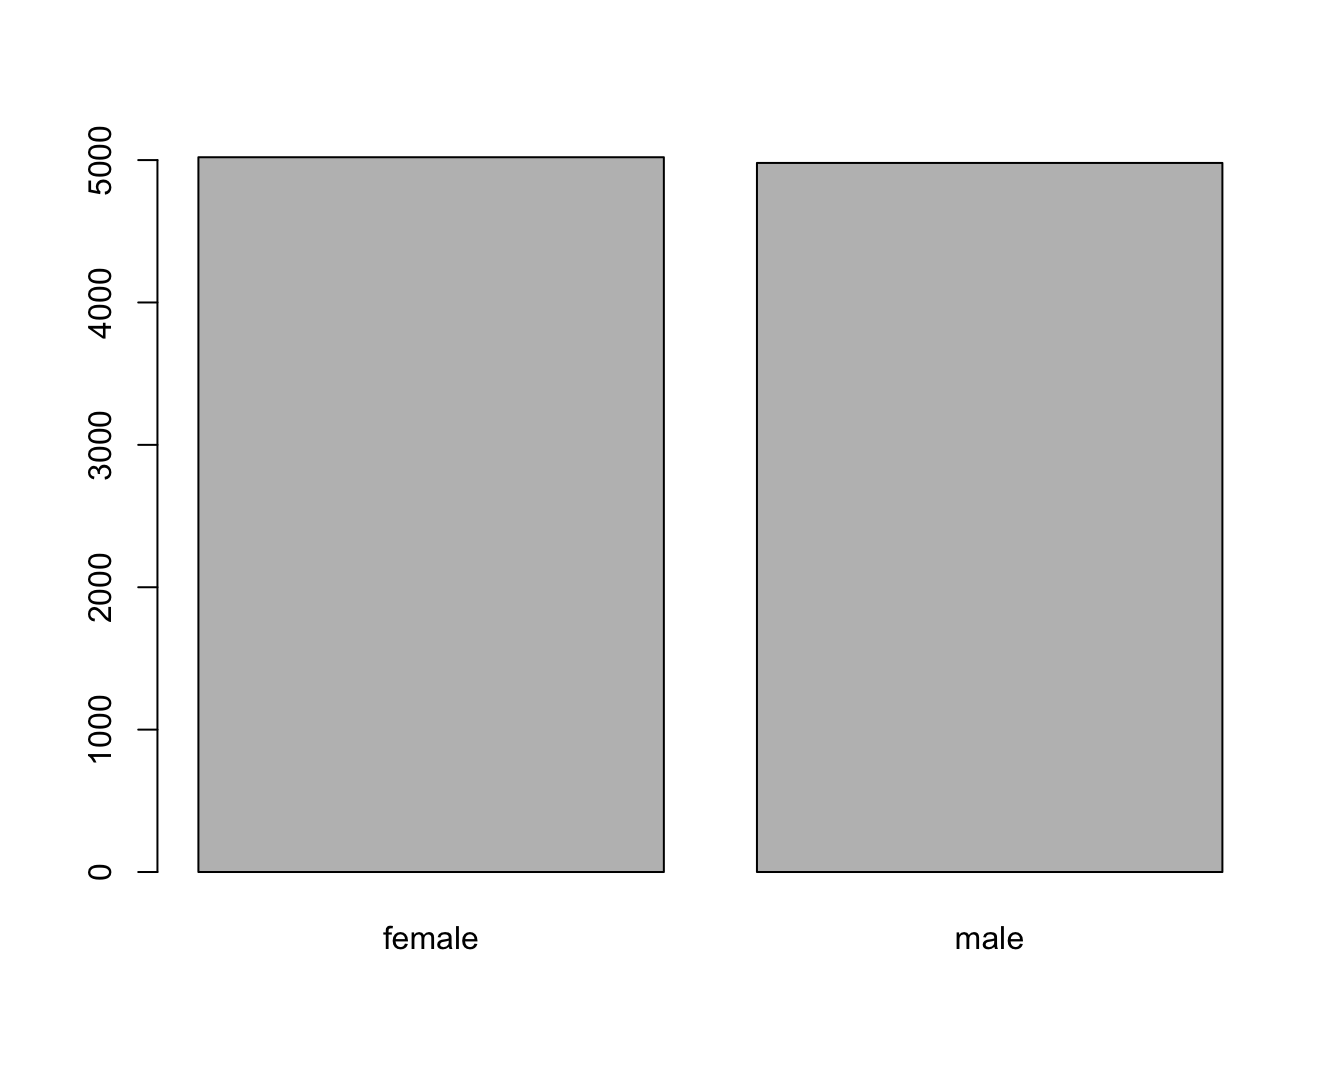
\includegraphics[width=1\linewidth]{Statistiek_2019_2020_files/figure-latex/fretabs-1} 

}

\caption{Staafdiagram van het aantal mannen en vrouwen in de NHANES studie.}\label{fig:fretabs}
\end{figure}

Er zijn weinig methoden voorhanden om \emph{nominale} variabelen te
beschrijven. In Voorbeeld \ref{exm:nhanesEx} is de variable
\emph{Gender} kwalitatief nominaal. Alles is gezegd over de verdeling
van het geslacht als we weergeven hoeveel vrouwen en mannen zijn
opgenomen in de studie. Meer nog, als het totale aantal personen in de
data set eenmaal vast ligt, dan zijn de uitkomsten verder volledig
gekarakteriseerd door, bijvoorbeeld, alleen het percentage vrouwen en
mannen weergeen. In het softwarepakket R kan men een beeld van de
gegevens krijgen door ze in een \emph{frequentietabel} weer te geven of
a.d.h.v. een grafiek zoals een \emph{staafdiagram}. Beiden worden
gegenereerd in de R-code voor Figuur \ref{fig:fretabs}. We stellen vast
dat 5020 van de 10000 subjecten, ofwel 50.2\% vrouwen in de studie zijn
opgenomen.

Een staafdiagram geeft op de X-as de mogelijke uitkomsten van de
variabele aan (bvb. geslacht). Daarbovenop komt een staaf met hoogte
evenredig aan het totaal aantal keer dat die waarde voorkomt in de
dataset. In het bijzonder kan men kiezen tussen de \emph{absolute
frequentie} (5020 voor het aantal vrouwen, 4980 voor het aantal mannen)
of de \emph{relatieve frequentie} ( 50.2\% vrouwen, 49.8\% mannen). De
staven staan los van elkaar met een breedte die constant is, maar verder
willekeurig. Als de steekproef representatief is voor de populatie, dan
krijgen we hier misschien een eerste impressie dat er iets meer vrouwen
zijn in de populatie.

De variabele met de naam \emph{BMI\_WHO} in de dataset is kwalitatief
ordinaal en heeft 4 geordende categorieën die grensen voor ondergewicht,
normaal gewicht, licht-overgewicht, obesitas. Voor dergelijke ordinale
variabelen worden de mogelijke uitkomsten best in volgorde gesorteerd en
in een frequentietabel of staafdiagram weergegeven. Naast de (relatieve)
frequentie is het nu ook zinvol om de \emph{cumulatieve (relatieve)
frequentie} aan te geven. Deze laatste drukt uit welk percentage van de
gegevens in de gegeven klasse of een lagere klasse valt. In Figuur
\ref{fig:freqmilt} vind je het staafdiagram voor het BMI. In de R-code
voor de figuur vind je tevens de bijhorende frequentietabel.

\begin{Shaded}
\begin{Highlighting}[]
\CommentTok{# sla freq. tabel op in object 'tabBmi'}
\NormalTok{tabBmi <-}\StringTok{ }\KeywordTok{table}\NormalTok{(NHANES}\OperatorTok{$}\NormalTok{BMI_WHO)}
\NormalTok{tabBmi}
\end{Highlighting}
\end{Shaded}

\begin{verbatim}
## 
##    12.0_18.5 18.5_to_24.9 25.0_to_29.9    30.0_plus 
##         1277         2911         2664         2751
\end{verbatim}

\begin{Shaded}
\begin{Highlighting}[]
\CommentTok{# teken staaf diagram}
\KeywordTok{barplot}\NormalTok{(tabBmi)}
\end{Highlighting}
\end{Shaded}

\begin{figure}

{\centering 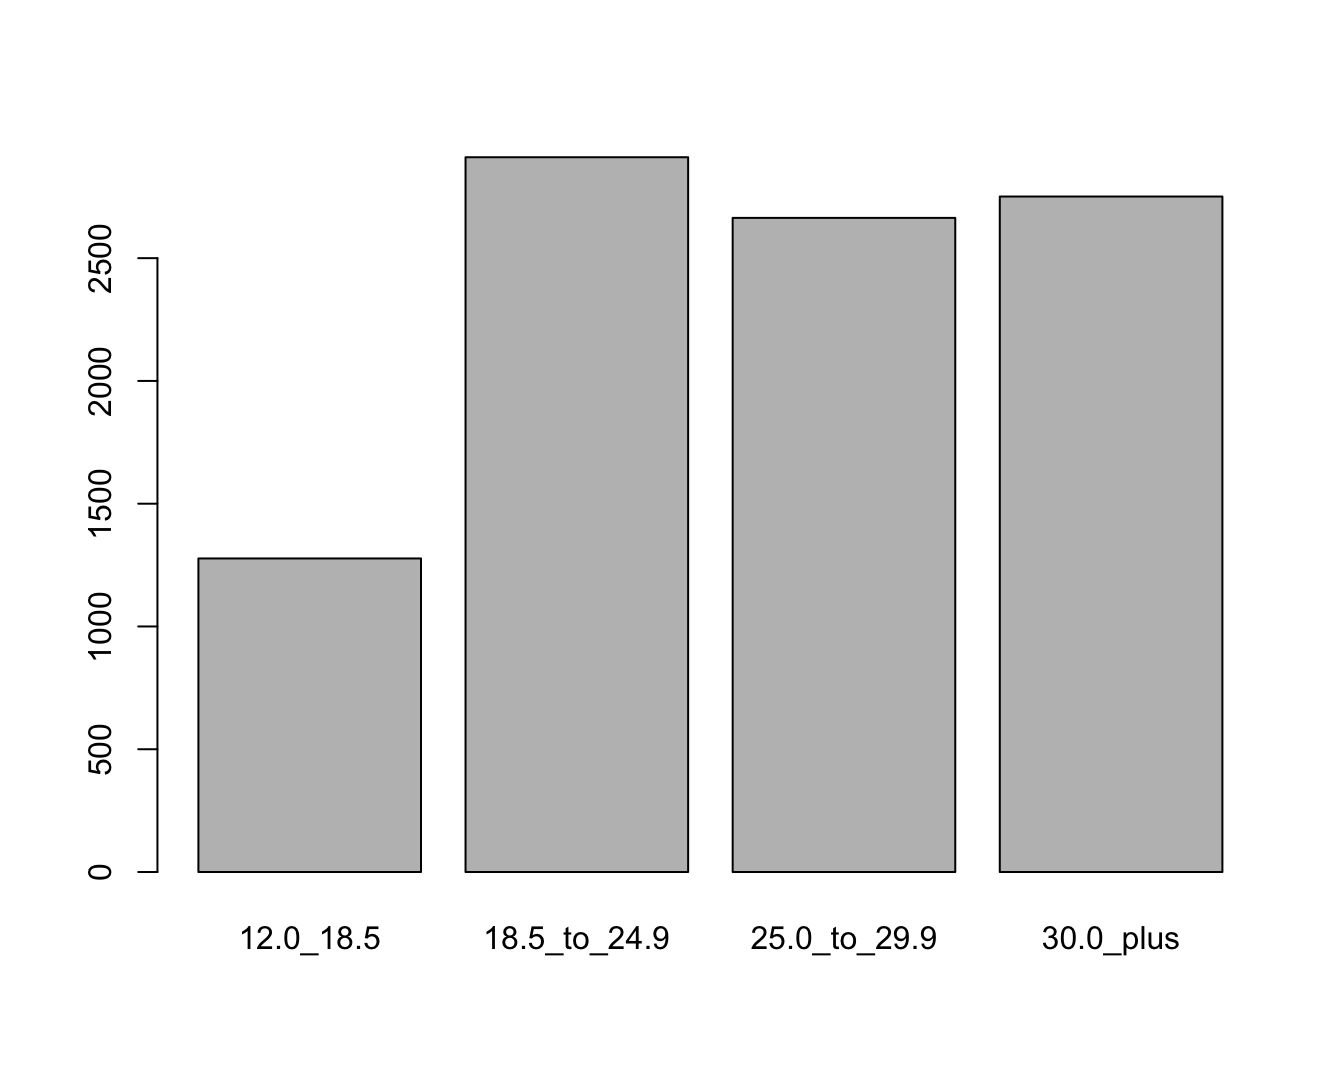
\includegraphics[width=1\linewidth]{Statistiek_2019_2020_files/figure-latex/freqmilt-1} 

}

\caption{Staafdiagram van het aantal personen in de NHANES studie die behoort tot elke BMI klasse.}\label{fig:freqmilt}
\end{figure}

Voor \emph{numerieke continue variabelen} wordt het moeilijk om de
frequentie van alle uitkomstwaarden in een tabel te klasseren omdat veel
waarden hoogstens 1 keer voorkomen. Het \emph{tak-en-blad diagram} (in
het Engels: \emph{stem and leaf plot} is een middel om toch nog alle
uitkomsten weer te geven. Een voorbeeld is weergegeven in onderstaande
R-output voor het BMI in de NHANES studie.

\begin{Shaded}
\begin{Highlighting}[]
\KeywordTok{stem}\NormalTok{(NHANES}\OperatorTok{$}\NormalTok{BMI)}
\end{Highlighting}
\end{Shaded}

\begin{verbatim}
## 
##   The decimal point is 1 digit(s) to the right of the |
## 
##   1 | 33333333333333333344444444444444444444444444444444444444444444444444+37
##   1 | 55555555555555555555555555555555555555555555555555555555555555555555+1389
##   2 | 00000000000000000000000000000000000000000000000000000000000000000000+2264
##   2 | 55555555555555555555555555555555555555555555555555555555555555555555+2610
##   3 | 00000000000000000000000000000000000000000000000000000000000000000000+1693
##   3 | 55555555555555555555555555555555555555555555555555555555555555555555+635
##   4 | 00000000000000000000000000000000000000000000000000000000000000000000+255
##   4 | 55555555555555555555555556666666666666666666666666666666666777777777+46
##   5 | 0000011111122222233333444444444444
##   5 | 5556677777789999
##   6 | 133444
##   6 | 567899
##   7 | 
##   7 | 
##   8 | 111
\end{verbatim}

Hier wordt van alle uitkomsten het eerste cijfer of de eerste paar
cijfers op een verticale lijn in volgorde uitgezet in de vorm van een
boomstam. Daaraan worden horizontaal de bladeren gehecht, met name de
laatste cijfers van de geobserveerde uitkomsten. De output geeft
bijvoorbeeld aan dat er 3 personen zijn waarvan het afgeronde BMI 55
bedraagt, 2 personen met een afgerond BMI van 56, \ldots{}. Gezien de
studie zo groot is, is het tak-en-blad diagram niet erg praktisch voor
dit voorbeeld.

In een tak-en-blad diagram krijgt men alle individuele uitkomsten
nagenoeg exact te zien, terwijl de vorm die het diagram aanneemt reeds
een idee van de verdeling geeft zoals in een histogram (zie verder). Een
vuistregel om de vorm van de verdeling het best te zien is het aantal
takken ongeveer gelijk te maken aan \(1 + \sqrt{n}\), waarbij \(n\) het
aantal observaties voorstelt. Dit aantal kan uiteraard aangepast worden
aan de omstandigheden. Een populair alternatief voor het tak en blad
diagram is de \emph{eenvoudige frequentietabel}. Deze kan men bekomen
door de continue variabele (bvb. BMI) om te zetten in een kwalitatieve
ordinale variabele, waarvoor vervolgens een frequentietabel wordt
weergegeven. Merk op dat dit voor het BMI eerst is gebeurd (Figuur
\ref{fig:freqmilt}).

Het grafisch equivalent van dergelijke frequentietabel noemt een
\emph{histogram}, hetgeen men in R bekomt via

\begin{Shaded}
\begin{Highlighting}[]
\KeywordTok{hist}\NormalTok{(NHANES}\OperatorTok{$}\NormalTok{BMI, }\DataTypeTok{main =} \StringTok{""}\NormalTok{, }\DataTypeTok{xlab =} \StringTok{"BMI"}\NormalTok{)  }\CommentTok{#main is hoofdtitel}
\end{Highlighting}
\end{Shaded}

\begin{figure}

{\centering 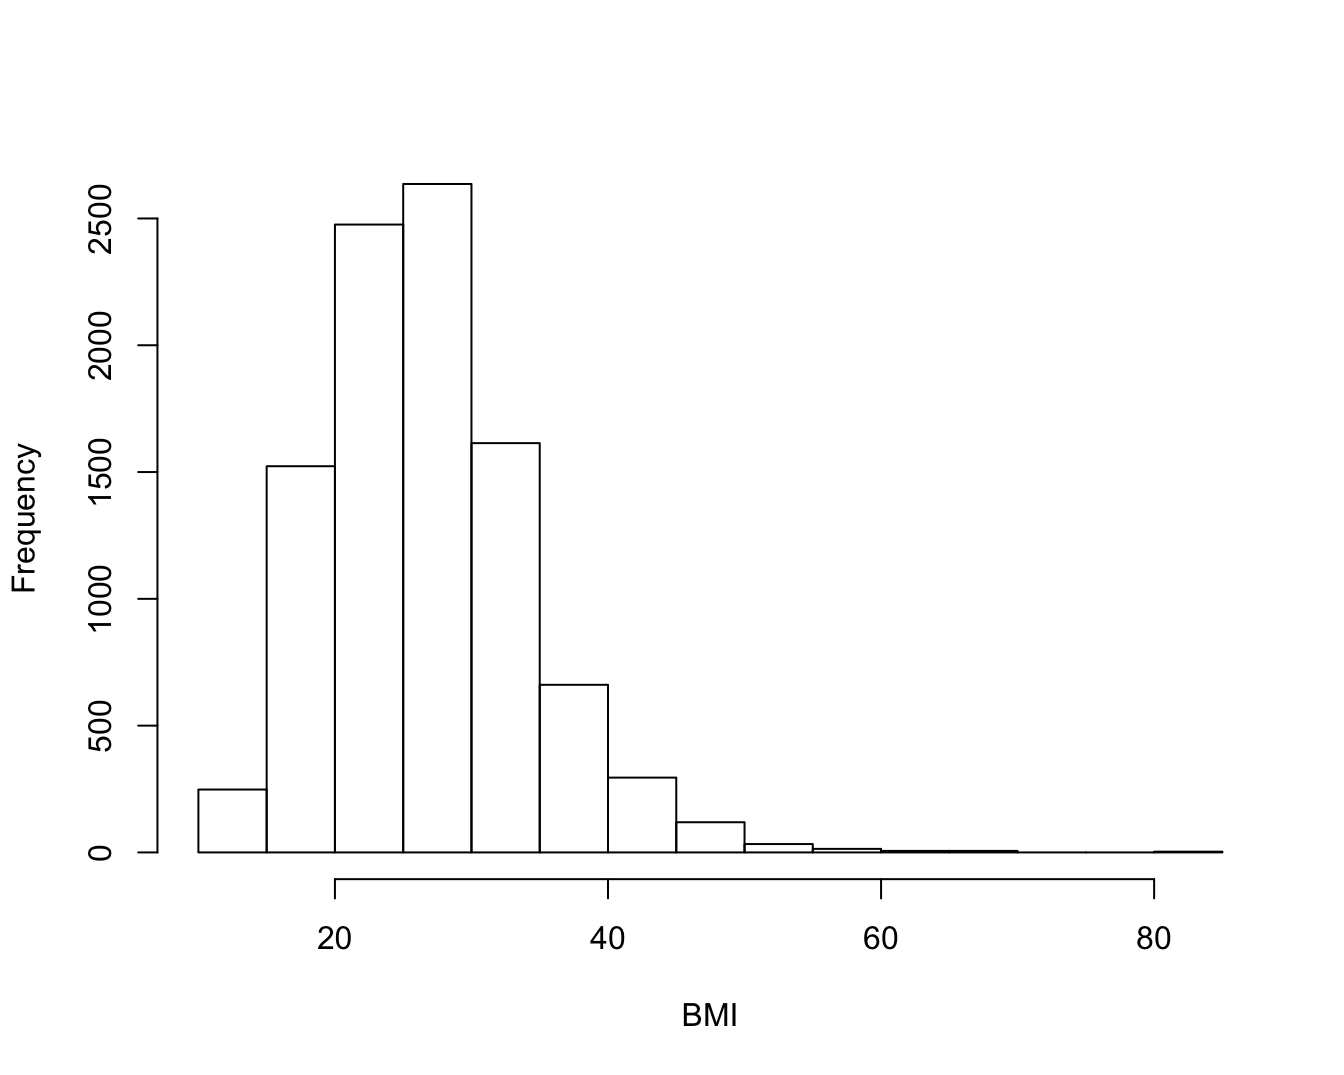
\includegraphics[width=1\linewidth]{Statistiek_2019_2020_files/figure-latex/histo-1} 

}

\caption{Histogram van het BMI in de NHANES studie.}\label{fig:histo}
\end{figure}

Wanneer alle klassen een zelfde breedte hebben, worden de absolute of
relatieve frequenties per klasse weergegeven door de hoogte van de
bijhorende kolom. Bij ongelijke klassebreedtes is het de oppervlakte van
de kolom die met de bijhorende klassefrequentie correspondeert. Omdat
een histogram met ongelijke klassebreedtes moeilijker te interpreteren
is, zijn histogrammen met gelijke klassebreedtes vaak te verkiezen. Als
histogrammen voor verschillende groepen bekeken worden, vergemakkelijkt
het gebruik van \emph{relatieve} frequenties i.p.v. absolute frequenties
de visuele vergelijkbaarheid.

Op het histogram in Figuur \ref{fig:histo} worden absolute frequenties
weergegeven en klassen met een breedte van 5 eenheden. We stellen vast
dat ongeveer 1500 personen van de 10000, of 15\% een BMI heeft tussen de
15 en 20.

De keuze van het aantal klassen is van belang bij een histogram. Als er
te weinig klassen zijn, dan gaat veel informatie verloren. Als er teveel
zijn, dan wordt het algemene patroon verdoezeld door een grote
hoeveelheid overbodige details. Gewoonlijk kiest men tussen 5 en 15
intervallen, maar de specifieke keuze hangt af van het beeld van het
histogram dat men te zien krijgt.

Indien een voldoende aantal gegevens beschikbaar is, dan kan men een
gladdere indruk van de verdeling van de gegevens bekomen door een
zogenaamde \emph{kernel density schatter} te bepalen. Zo'n schatter is
een positieve functie die genormaliseerd is in die zin dat de
oppervlakte onder de functie 1 is. Ze kan zo geïnterpreteerd worden dat
de oppervlakte onder de functie tussen 2 punten \(a\) en \(b\) op de
X-as, de kans voorstelt dat een lukrake meting in het interval \([a,b]\)
gevonden wordt. Figuur \ref{fig:freqpoly} toont een histogram (links) en
kernel density schatter (rechts) van de het BMI.

\begin{Shaded}
\begin{Highlighting}[]
\CommentTok{# deel grafische scherm op in 1 rij en 2 kolommen}
\KeywordTok{par}\NormalTok{(}\DataTypeTok{mfrow =} \KeywordTok{c}\NormalTok{(}\DecValTok{1}\NormalTok{, }\DecValTok{2}\NormalTok{))}
\CommentTok{# teken een histogram}
\KeywordTok{hist}\NormalTok{(NHANES}\OperatorTok{$}\NormalTok{BMI, }\DataTypeTok{main =} \StringTok{""}\NormalTok{, }\DataTypeTok{xlab =} \StringTok{"BMI"}\NormalTok{)}
\CommentTok{# teken een kernel density schatter}
\KeywordTok{plot}\NormalTok{(}\KeywordTok{density}\NormalTok{(NHANES}\OperatorTok{$}\NormalTok{BMI, }\DataTypeTok{na.rm =} \OtherTok{TRUE}\NormalTok{), }\DataTypeTok{main =} \StringTok{""}\NormalTok{, }
    \DataTypeTok{xlab =} \StringTok{"BMI"}\NormalTok{)}
\end{Highlighting}
\end{Shaded}

\begin{figure}

{\centering 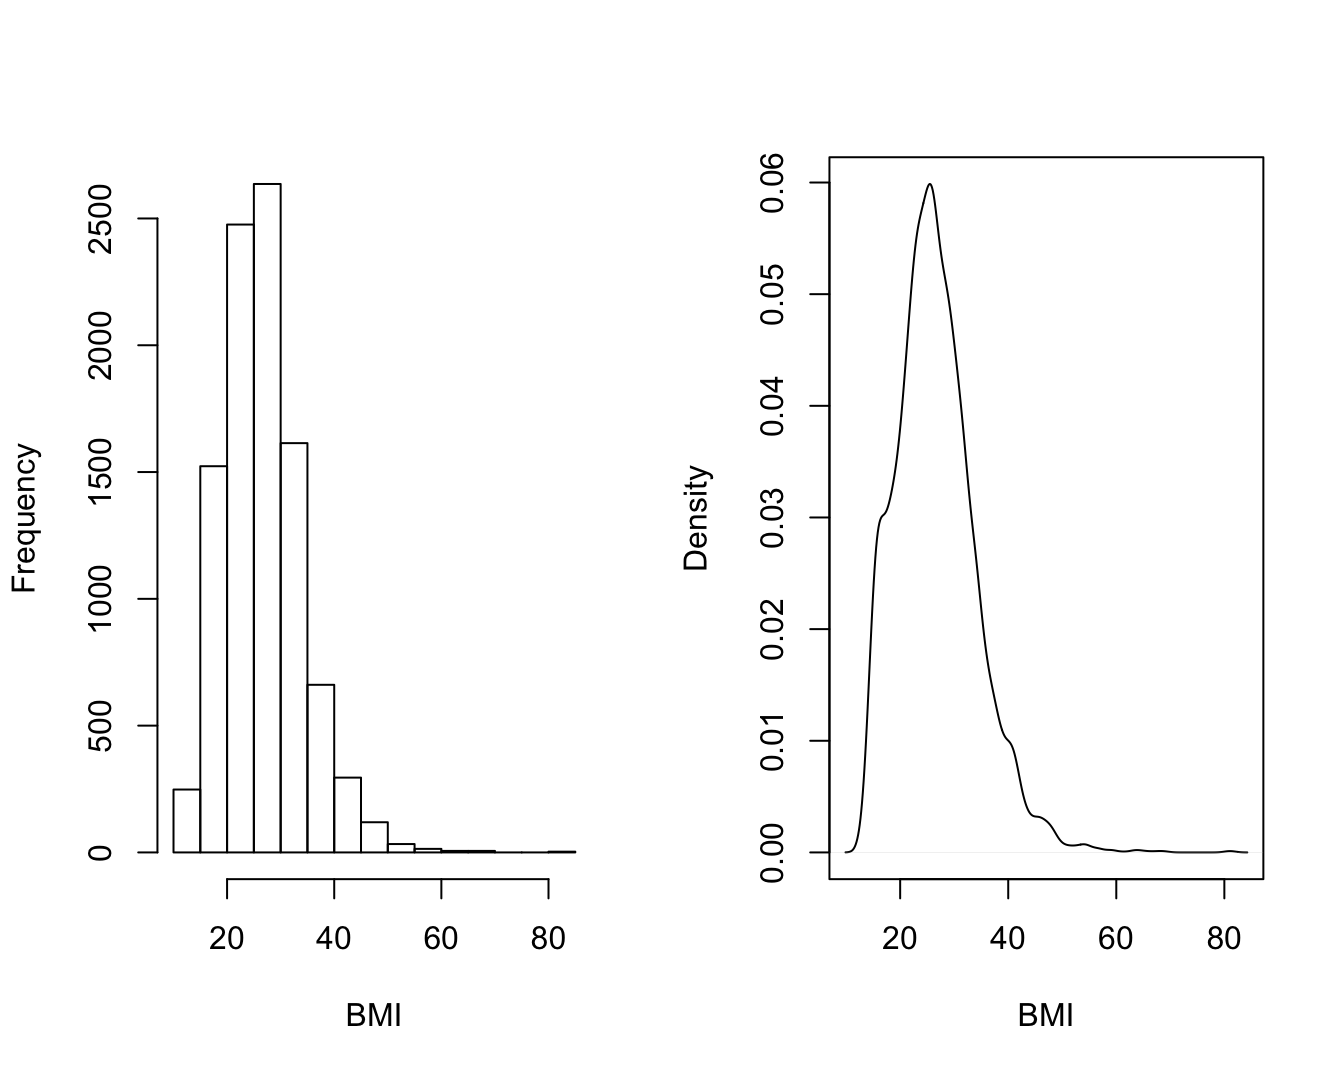
\includegraphics[width=1\linewidth]{Statistiek_2019_2020_files/figure-latex/freqpoly-1} 

}

\caption{Histogram en kernel density schatter van BMI in de NHANES studie.}\label{fig:freqpoly}
\end{figure}

\begin{Shaded}
\begin{Highlighting}[]
\CommentTok{# argument na.rm=TRUE omdat er ontbrekende}
\CommentTok{# waarnemingen (NA) voorkomen}
\end{Highlighting}
\end{Shaded}

De verdeling kan ook geëvalueerd worden aan de hand van een
\emph{box-and-whisker-plot}, kortweg \emph{boxplot} genoemd. Deze is
meer compact dan een histogram en laat om die reden gemakkelijker
vergelijkingen tussen verschillende groepen toe (zie verder). Een
Boxplot voor het BMI wordt getoond in Figuur \ref{fig:boxBMI}. De
boxplot toont een doos lopend van het 25\% tot 75\% percentiel met een
lijntje ter hoogte van de mediaan (het 50\% percentiel) en verder 2
snorharen. Die laatste kunnen in principe lopen tot het minimum en
maximum, of tot het 2.5\% en 97.5 \% of 5\% en 95\% percentiel. R kiest
voor de kleinste en de grootste geobserveerde waarde die geen outlier of
extreme waarde zijn. Een meting wordt hierbij een outlier genoemd
wanneer ze meer dan 1.5 keer de boxlengte beneden het eerste of boven
het derde kwartiel ligt. Een meting wordt een extreme waarde genoemd
wanneer ze meer dan 3 keer de boxlengte beneden het eerste of boven het
derde kwartiel ligt.

\BeginKnitrBlock{definition}[percentiel]
\protect\hypertarget{def:unnamed-chunk-35}{}{\label{def:unnamed-chunk-35}
\iffalse (percentiel) \fi{} }Het \emph{25\% percentiel} of \emph{25\%
kwantiel} \(x_{25}\) van een reeks waarnemingen wordt gedefinieerd als
een uitkomstwaarde \(x_{25}\) zodat minstens \(25\%\) van die
waarnemingen kleiner of gelijk zijn aan \(x_{25}\) en minstens \(75\%\)
van die waarnemingen groter of gelijk zijn aan \(x_{25}\). Het
\emph{75\% percentiel} of \emph{75\% kwantiel} van een reeks
waarnemingen definieert men als een uitkomstwaarde \(x_{75}\) zodat
minstens 75\% kleiner of gelijk zijn aan \(x_{75}\) en minstens \(25\%\)
van die waarnemingen groter of gelijk zijn aan \(x_{75}\). Algemeen
wordt het \emph{\(k\%\) percentiel} van een reeks waarnemingen
gedefinieerd als een waarde (van \(x\)) waarvoor de cumulatieve
frequentie gelijk is aan \(k/100.\) Als er meerdere observaties aan
voldoen neemt men vaak het gemiddelde van die waarden.

\textbf{Einde definitie}
\EndKnitrBlock{definition}

In R kunnen die als volgt worden bekomen

\begin{Shaded}
\begin{Highlighting}[]
\KeywordTok{quantile}\NormalTok{(NHANES}\OperatorTok{$}\NormalTok{BMI, }\KeywordTok{c}\NormalTok{(}\FloatTok{0.25}\NormalTok{, }\FloatTok{0.5}\NormalTok{, }\FloatTok{0.75}\NormalTok{), }\DataTypeTok{na.rm =} \OtherTok{TRUE}\NormalTok{)}
\end{Highlighting}
\end{Shaded}

\begin{verbatim}
##   25%   50%   75% 
## 21.58 25.98 30.89
\end{verbatim}

\begin{Shaded}
\begin{Highlighting}[]
\CommentTok{# code om boxplot te genereren}
\KeywordTok{boxplot}\NormalTok{(NHANES}\OperatorTok{$}\NormalTok{BMI, }\DataTypeTok{ylab =} \StringTok{"BMI"}\NormalTok{)}

\CommentTok{# Code om text toe te voegen aan plot Dit hoef je}
\CommentTok{# zelf normaal gezien niet te doen}
\NormalTok{BMI =}\StringTok{ }\KeywordTok{na.exclude}\NormalTok{(NHANES}\OperatorTok{$}\NormalTok{BMI)}
\NormalTok{rangeCl <-}\StringTok{ }\KeywordTok{quantile}\NormalTok{(BMI, }\KeywordTok{c}\NormalTok{(}\FloatTok{0.25}\NormalTok{, }\FloatTok{0.75}\NormalTok{)) }\OperatorTok{+}\StringTok{ }\KeywordTok{c}\NormalTok{(}\OperatorTok{-}\DecValTok{1}\NormalTok{, }\DecValTok{1}\NormalTok{) }\OperatorTok{*}\StringTok{ }
\StringTok{    }\KeywordTok{diff}\NormalTok{(}\KeywordTok{quantile}\NormalTok{(BMI, }\KeywordTok{c}\NormalTok{(}\FloatTok{0.25}\NormalTok{, }\FloatTok{0.75}\NormalTok{))) }\OperatorTok{*}\StringTok{ }\FloatTok{1.5}
\NormalTok{boxYs <-}\StringTok{ }\KeywordTok{c}\NormalTok{(}\KeywordTok{range}\NormalTok{(BMI[BMI }\OperatorTok{<=}\StringTok{ }\NormalTok{rangeCl[}\DecValTok{2}\NormalTok{] }\OperatorTok{&}\StringTok{ }\NormalTok{BMI }\OperatorTok{>=}\StringTok{ }\NormalTok{rangeCl[}\DecValTok{1}\NormalTok{]]), }
    \KeywordTok{quantile}\NormalTok{(BMI, }\KeywordTok{c}\NormalTok{(}\FloatTok{0.25}\NormalTok{, }\FloatTok{0.5}\NormalTok{, }\FloatTok{0.75}\NormalTok{)), rangeCl[}\DecValTok{2}\NormalTok{] }\OperatorTok{+}\StringTok{ }
\StringTok{        }\NormalTok{(}\KeywordTok{max}\NormalTok{(BMI) }\OperatorTok{-}\StringTok{ }\NormalTok{rangeCl[}\DecValTok{2}\NormalTok{])}\OperatorTok{/}\DecValTok{2}\NormalTok{)}

\KeywordTok{text}\NormalTok{(}\FloatTok{1.3}\NormalTok{, boxYs, }\DataTypeTok{labels =} \KeywordTok{c}\NormalTok{(}\StringTok{"wisker"}\NormalTok{, }\StringTok{"wisker"}\NormalTok{, }\StringTok{"x25"}\NormalTok{, }
    \StringTok{"mediaan"}\NormalTok{, }\StringTok{"x75"}\NormalTok{, }\StringTok{"outliers"}\NormalTok{), }\DataTypeTok{pos =} \DecValTok{4}\NormalTok{, }\DataTypeTok{cex =} \FloatTok{1.3}\NormalTok{)}
\KeywordTok{lines}\NormalTok{(}\KeywordTok{c}\NormalTok{(}\FloatTok{1.1}\NormalTok{, }\FloatTok{1.3}\NormalTok{, }\FloatTok{1.3}\NormalTok{, }\FloatTok{1.1}\NormalTok{), }\KeywordTok{c}\NormalTok{(rangeCl[}\DecValTok{2}\NormalTok{], rangeCl[}\DecValTok{2}\NormalTok{] }\OperatorTok{+}\StringTok{ }
\StringTok{    }\NormalTok{(}\KeywordTok{max}\NormalTok{(BMI) }\OperatorTok{-}\StringTok{ }\NormalTok{rangeCl[}\DecValTok{2}\NormalTok{])}\OperatorTok{/}\DecValTok{2}\NormalTok{, rangeCl[}\DecValTok{2}\NormalTok{] }\OperatorTok{+}\StringTok{ }\NormalTok{(}\KeywordTok{max}\NormalTok{(BMI) }\OperatorTok{-}\StringTok{ }
\StringTok{    }\NormalTok{rangeCl[}\DecValTok{2}\NormalTok{])}\OperatorTok{/}\DecValTok{2}\NormalTok{, }\KeywordTok{max}\NormalTok{(BMI)), }\DataTypeTok{lty =} \DecValTok{2}\NormalTok{)}
\end{Highlighting}
\end{Shaded}

\begin{figure}

{\centering 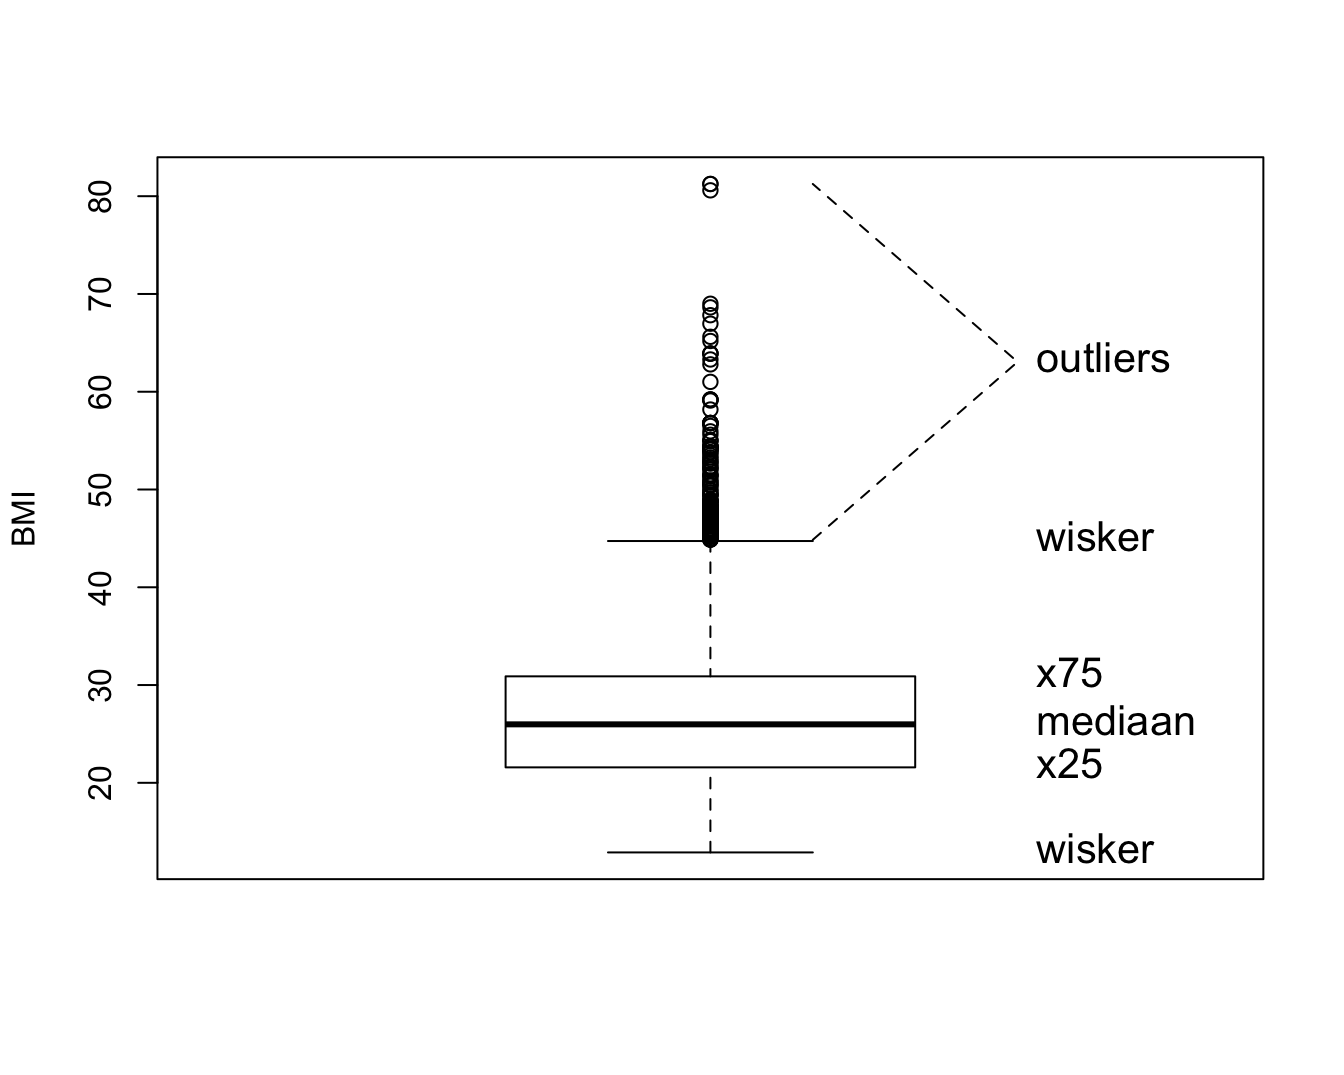
\includegraphics[width=1\linewidth]{Statistiek_2019_2020_files/figure-latex/boxBMI-1} 

}

\caption{Boxplot van BMI in de NHANES studie.}\label{fig:boxBMI}
\end{figure}

Bij de inspectie van een dataset speelt het detecteren van outliers in
het algemeen een belangrijke rol. Ze kunnen wijzen op fouten, zoals
tikfouten of andere fouten die gecheckt en gecorrigeerd moeten worden.
Als het geen foutief genoteerde waarden zijn, dan kan het soms wijzen op
een subject dat niet echt in de studiepopulatie thuis hoort. Als het in
alle opzichten om een bona fide waarde gaat, dan nog is het belangrijk
om outliers te detecteren: ze kunnen zeer invloedrijk zijn op de
schatting van statistische parameters (zie Sectie \ref{sec:summarize}).
Als de conclusies van een studie anders liggen met of zonder inclusie
van de outlier, dan is dit een ongewenst fenomeen. Men wil immers nooit
dat 1 observatie beslissend is voor de conclusies. Dit soort onzekerheid
ondermijnt de geloofwaardigheid van de onderzoeksresultaten en vraagt om
verdere studie. Binnen de statistiek bestaat een grote waaier aan
technieken, zogenaamde \emph{robuuste statistische technieken}, die erop
gericht zijn om de invloed van outliers te minimaliseren. In deze cursus
gaan we hier slechts in zeer beperkte mate op in (zie Sectie
\ref{sec:summarize}, mediaan).

\section{Samenvattingsmaten voor continue
variabelen}\label{sec:summarize}

Een histogram levert reeds een sterke samenvatting van de geobserveerde,
continue gegevens, maar in wetenschappelijke rapporten is er zelden
plaats om per geobserveerde variabele dergelijke grafiek voor te
stellen. Om die reden is vaak een veel drastischere samenvattingsmaat
noodzakelijk. In deze sectie geven we aan hoe de centrale locatie van de
gegevens kan beschreven worden, alsook de spreiding van die gegevens
rond hun centrale locatie.

\subsection{Maten voor de centrale
ligging}\label{maten-voor-de-centrale-ligging}

\BeginKnitrBlock{definition}[rekenkundig gemiddelde]
\protect\hypertarget{def:unnamed-chunk-37}{}{\label{def:unnamed-chunk-37}
\iffalse (rekenkundig gemiddelde) \fi{} }Het \textbf{(rekenkundig)
gemiddelde} \(\overline{x}\) (spreek uit: \emph{x-streep} of
\emph{x-bar}) van een reeks waarnemingen \(x_i, i=1, 2, \dots, n\) is
per definitie de som van de observaties gedeeld door hun aantal \(n\):

\begin{equation*}
\overline{x}= \frac{x_1 + x_2 + \dots + x_n}{n} =\frac{1}{n} \sum_{i=1}^n x_i
\end{equation*}

\textbf{Einde definitie}
\EndKnitrBlock{definition}

Een groot voordeel van het gemiddelde als een maat voor de centrale
locatie van de observaties is dat het alle data-waarden efficiënt
gebruikt vanuit statistisch perspectief. Dit wil zeggen dat ze (onder
bepaalde statistische modellen) het maximum aan informatie uit de
gegevens haalt en om die reden relatief gezien zeer stabiel blijft
wanneer ze herberekend wordt op basis van een nieuwe, even grote
steekproef die onder identieke omstandigheden werd bekomen. Bovendien
beschrijft het gemiddelde ook verschillende belangrijke modellen voor de
verdeling van de gegevens, zoals de Normale verdeling (zie Sectie
\ref{sec:normal}). Een groot nadeel van het gemiddelde is dat het zeer
gevoelig is aan de aanwezigheid van outliers in de dataset. Om die reden
is het vooral een interessante maat van locatie wanneer de verdeling van
de observaties (zoals weergegeven door bijvoorbeeld een histogram) min
of meer symmetrisch is.

\begin{Shaded}
\begin{Highlighting}[]
\KeywordTok{mean}\NormalTok{(NHANES}\OperatorTok{$}\NormalTok{BMI, }\DataTypeTok{na.rm =} \OtherTok{TRUE}\NormalTok{)}
\end{Highlighting}
\end{Shaded}

\begin{verbatim}
## [1] 26.66014
\end{verbatim}

\begin{Shaded}
\begin{Highlighting}[]
\CommentTok{# opnieuw is de na.rm statement hier nodig omdat}
\CommentTok{# ontbrekende waarden voorkomen.}
\end{Highlighting}
\end{Shaded}

\emph{Indien men de grootste observatie (81.25) vervangt door 8125 om
als het ware ene tikfout voor te stellen, dan wijzigt het rekenkundig
gemiddelde naar 27.5 en dat terwijl er bijna 10000 BMI metingen zijn.
Merk op dat het gemiddelde vrij sterk beïnvloed kan worden door één
outlier.}

\textbf{Eigenschap}

Als alle uitkomsten \(x_i\) met een willekeurige constante \(a\) worden
vermenigvuldigd, dan ook het gemiddelde van die reeks uitkomsten. Als
bij alle uitkomsten een constante \(a\) wordt opgeteld, dan ook bij het
gemiddelde van die reeks uitkomsten. Formeel betekent dit:

\begin{eqnarray*}
\overline{ax} &= &a \overline{x} \\
\overline{a + x} &= &a + \overline{x}
\end{eqnarray*}

Voor 2 reeksen getallen \(x_i\) en \(y_i\), \(i=1,...,n\), geldt dat het
gemiddelde van de som van de observaties gelijk is aan de som van hun
gemiddelden:

\begin{equation*}
\overline{x + y} = \overline{x} + \overline{y}.
\end{equation*}

Als de gegevens \(x_i\) enkel de waarden 0 of 1 aannemen, dan is
\(\overline{x}\) de proportie subjecten voor wie de waarde 1 werd
geobserveerd. Immers, zij \(n_1\) het aantal subjecten binnen de groep
van \(n\) subjecten waarvoor de waarde 1 werd geobserveerd, dan is

\begin{equation*}
\overline{x}= \sum_{i=1}^n \frac{x_i}{n} = \frac{n_1}{n}.
\end{equation*}

Bijvoorbeeld, als we de variabele \textbf{Gender} zó coderen dat mannen
een waarde 0 aannemen en vrouwen een waarde 1, dan is het gemiddelde van
de variabele \textbf{Gender} gelijk aan 50.2\%, hetgeen de proportie is
van het aantal vrouwen in de studie. Een percentage kan dus steeds
opgevat worden als het gemiddelde van een geschikte variabele.

\textbf{Einde eigenschap}

Een centrale maat die robuuster reageert dan het gemiddelde, d.w.z.
minder of niet gevoelig is aan outliers, is de \emph{mediaan} of het
\emph{50\% percentiel}.

\BeginKnitrBlock{definition}[mediaan]
\protect\hypertarget{def:unnamed-chunk-39}{}{\label{def:unnamed-chunk-39}
\iffalse (mediaan) \fi{} }De \textbf{mediaan}, het \textbf{50\%
percentiel} of het \textbf{50\% kwantiel} \(x_{50}\) van een reeks
waarnemingen \(x_i, i=1, 2, \dots, n\) is per definitie een
uitkomstwaarde \(x_{50}\) zodat minstens \(50\%\) van die waarnemingen
groter of gelijk zijn aan \(x_{50}\) en minstens \(50\%\) van die
waarnemingen kleiner of gelijk zijn aan \(x_{50}\).

\textbf{Einde definitie}
\EndKnitrBlock{definition}

Om de mediaan te schatten, rangschikt men eerst de gegevens volgens
grootte. Als het aantal observaties \(n\) oneven is, dan is een
schatting voor de mediaan de middelste waarneming. Indien \(n\) even is,
dan zijn er 2 middelste waarnemingen en schat men de mediaan (meestal)
als hun gemiddelde. Een voordeel van de mediaan is dat ze niet gevoelig
is aan outliers. In het bijzonder kan ze vaak nuttig aangewend worden
wanneer sommige gegevens \emph{gecensureerd} zijn. Dit wil zeggen dat
men voor een aantal gegevens enkel weet dat ze boven of onder een
bepaalde drempelwaarde liggen.

\begin{Shaded}
\begin{Highlighting}[]
\KeywordTok{median}\NormalTok{(NHANES}\OperatorTok{$}\NormalTok{BMI, }\DataTypeTok{na.rm =} \OtherTok{TRUE}\NormalTok{)}
\end{Highlighting}
\end{Shaded}

\begin{verbatim}
## [1] 25.98
\end{verbatim}

\begin{Shaded}
\begin{Highlighting}[]
\CommentTok{# Merk op dat we hier gebruik maken van het}
\CommentTok{# argument na.rm=TRUE Dit komt omdat we niet}
\CommentTok{# beschikken over het BMI voor elke persoon:}
\CommentTok{# ontbrekende waarnemingen Die worden in R als een}
\CommentTok{# NA voorgesteld Als we het argument na.rm=TRUE}
\CommentTok{# gebruiken wordt de mediaan berekend op basis van}
\CommentTok{# de beschikbare observaties}
\end{Highlighting}
\end{Shaded}

Indien men de grootste observatie (81.25) vervangt 8125, dan wijzigt de
mediaan niet. Merk ook op dat de mediaan lager is dan het gemiddelde,
hij is minder gevoelig voor de outliers in de dataset.

\BeginKnitrBlock{definition}[modus]
\protect\hypertarget{def:unnamed-chunk-41}{}{\label{def:unnamed-chunk-41}
\iffalse (modus) \fi{} }De \textbf{modus} van een reeks observaties is
de waarde die het meest frequent is, of wanneer de gegevens gegroepeerd
worden, de klasse met de hoogste frequentie.

\textbf{Einde definitie}
\EndKnitrBlock{definition}

De modus wordt niet vaak gebruikt in statistische analyse omdat haar
waarde sterk afhangt van de nauwkeurigheid waarmee de gegevens werden
gemeten. Zo is de modus van de reeks observaties
\(1, 1, 1, 1.5, 1.75, 1.9, 2, 2.1, 2.4\) gelijk aan 1, maar wordt ze 2
wanneer alle observaties afgerond worden tot gehele getallen. Bovendien
is de modus niet eenvoudig te schatten voor continue data waar de
frequentie van elke geobserveerde waarde meestal 1 is. De modus is
daarom het meest zinvol voor kwalitatieve en discrete numerieke
gegevens, waar ze de meest frequente klasse aanduidt.

Als de observaties uit een \emph{symmetrische verdeling} afkomstig zijn,
vallen de mediaan en het gemiddelde nagenoeg samen (als de geobserveerde
verdeling perfect symmetrisch is, vallen ze theoretisch exact samen). De
beste schatter voor het centrum van de verdeling op basis van de
beschikbare steekproef is dan het gemiddelde eerder dan de mediaan van
die observaties. Inderdaad, als men telkens opnieuw een lukrake
steekproef neemt uit de gegeven studiepopulatie en voor elke steekproef
het gemiddelde en de mediaan berekent, dan zal het gemiddelde minder
variëren van steekproef tot steekproef dan de mediaan. Ze is bijgevolg
stabieler en wordt daarom een \emph{meer precieze schatter} genoemd.
Intuïtief kan men begrijpen dat het gemiddelde meer informatie uit de
gegevens gebruikt: niet alleen of iets groter of kleiner is dan
\(x_{50}\) maar ook hoeveel groter of kleiner de exacte waarde van elke
observatie is, wordt in de berekening betrokken.

\BeginKnitrBlock{definition}[scheve verdeling]
\protect\hypertarget{def:unnamed-chunk-42}{}{\label{def:unnamed-chunk-42}
\iffalse (scheve verdeling) \fi{} }Een niet-symmetrische verdeling wordt
\textbf{scheef} genoemd. Als de waarden rechts van de mediaan verder
uitlopen dan links, dan is de verdeling \emph{scheef naar rechts} (in
het Engels: \emph{positively skew}) en is het gemiddelde (meestal)
groter dan de mediaan. Als de waarden links van de mediaan verder
uitlopen dan rechts, dan is de verdeling \emph{scheef naar links} (in
het Engels: \emph{negatively skew}) en is het gemiddelde (meestal)
kleiner dan de mediaan.

\textbf{Einde definitie}
\EndKnitrBlock{definition}

Voor een niet-symmetrische verdeling is de mediaan veelal een beter
interpreteerbare maat dan het gemiddelde omdat ze minder beïnvloed is
door de staarten van de verdeling en daarom beter het centrum van de
verdeling aanduidt. Maar in sommige gevallen, zoals bijvoorbeeld voor
`de gemiddelde opbrengst per week', blijft het gemiddelde zinvol omdat
het meteen verwijst naar de totale opbrengst over alle weken (gelijk aan
\(n\) keer het gemiddelde als \(n\) weken werden geobserveerd). Ook voor
kwalitatieve variabelen kan een gemiddelde zinvol zijn. Voor binaire
nominale variabelen die als 1 of 0 gecodeerd zijn, geeft het gemiddelde
immers het percentage observaties gelijk aan 1 weer. Voor ordinale
variabelen die bijvoorbeeld gecodeerd zijn als \(1, 2, 3, ...\) levert
het gemiddelde soms nuttigere informatie dan de mediaan. Niettemin
berust het dan op de impliciete onderstelling dat een wijziging van
score van 1 naar 2 even belangrijk is als een wijziging van 2 naar 3.

Om scheve verdelingen in een paar woorden te beschrijven is het vaak
nuttig om

\begin{itemize}
\tightlist
\item
  ofwel de gegevens te beschrijven in termen van percentielen,
\item
  ofwel de gegevens te transformeren naar een andere schaal (bvb. door
  logaritmen te nemen), zodat ze op de nieuwe schaal bij benadering
  symmetrisch verdeeld zijn.
\end{itemize}

Wanneer het gemiddelde groter is dan de mediaan en alle metingen
positief zijn (vb concentraties, BMI), dan is een logaritmische
transformatie van de gegevens vaak nuttig om de scheefheid weg te nemen.
In dit geval is vooral het \emph{geometrisch gemiddelde} interessant.

\BeginKnitrBlock{definition}[geometrisch gemiddelde]
\protect\hypertarget{def:unnamed-chunk-43}{}{\label{def:unnamed-chunk-43}
\iffalse (geometrisch gemiddelde) \fi{} }Het \textbf{geometrische
gemiddelde} van een reeks waarnemingen \(x_i, i=1, 2, \dots, n\)
ontstaat door er de natuurlijke logaritme van te berekenen, het
gemiddelde hiervan te nemen en dit vervolgens terug te transformeren
naar de originele schaal door er de exponentiële functie van te nemen:

\begin{equation*}
\exp\left\{\frac{1}{n} \sum_{i=1}^n \log(x_i)\right\}
\end{equation*}

\textbf{Einde definitie}
\EndKnitrBlock{definition}

\begin{Shaded}
\begin{Highlighting}[]
\KeywordTok{par}\NormalTok{(}\DataTypeTok{mfrow =} \KeywordTok{c}\NormalTok{(}\DecValTok{1}\NormalTok{, }\DecValTok{2}\NormalTok{))}
\KeywordTok{hist}\NormalTok{(NHANES}\OperatorTok{$}\NormalTok{BMI, }\DataTypeTok{main =} \StringTok{"histogram van BMI"}\NormalTok{, }\DataTypeTok{xlab =} \StringTok{"BMI"}\NormalTok{)}
\KeywordTok{hist}\NormalTok{(}\KeywordTok{log}\NormalTok{(NHANES}\OperatorTok{$}\NormalTok{BMI), }\DataTypeTok{main =} \StringTok{"histogram van log(BMI)"}\NormalTok{, }
    \DataTypeTok{xlab =} \StringTok{"log(BMI)"}\NormalTok{)}
\end{Highlighting}
\end{Shaded}

\begin{figure}

{\centering 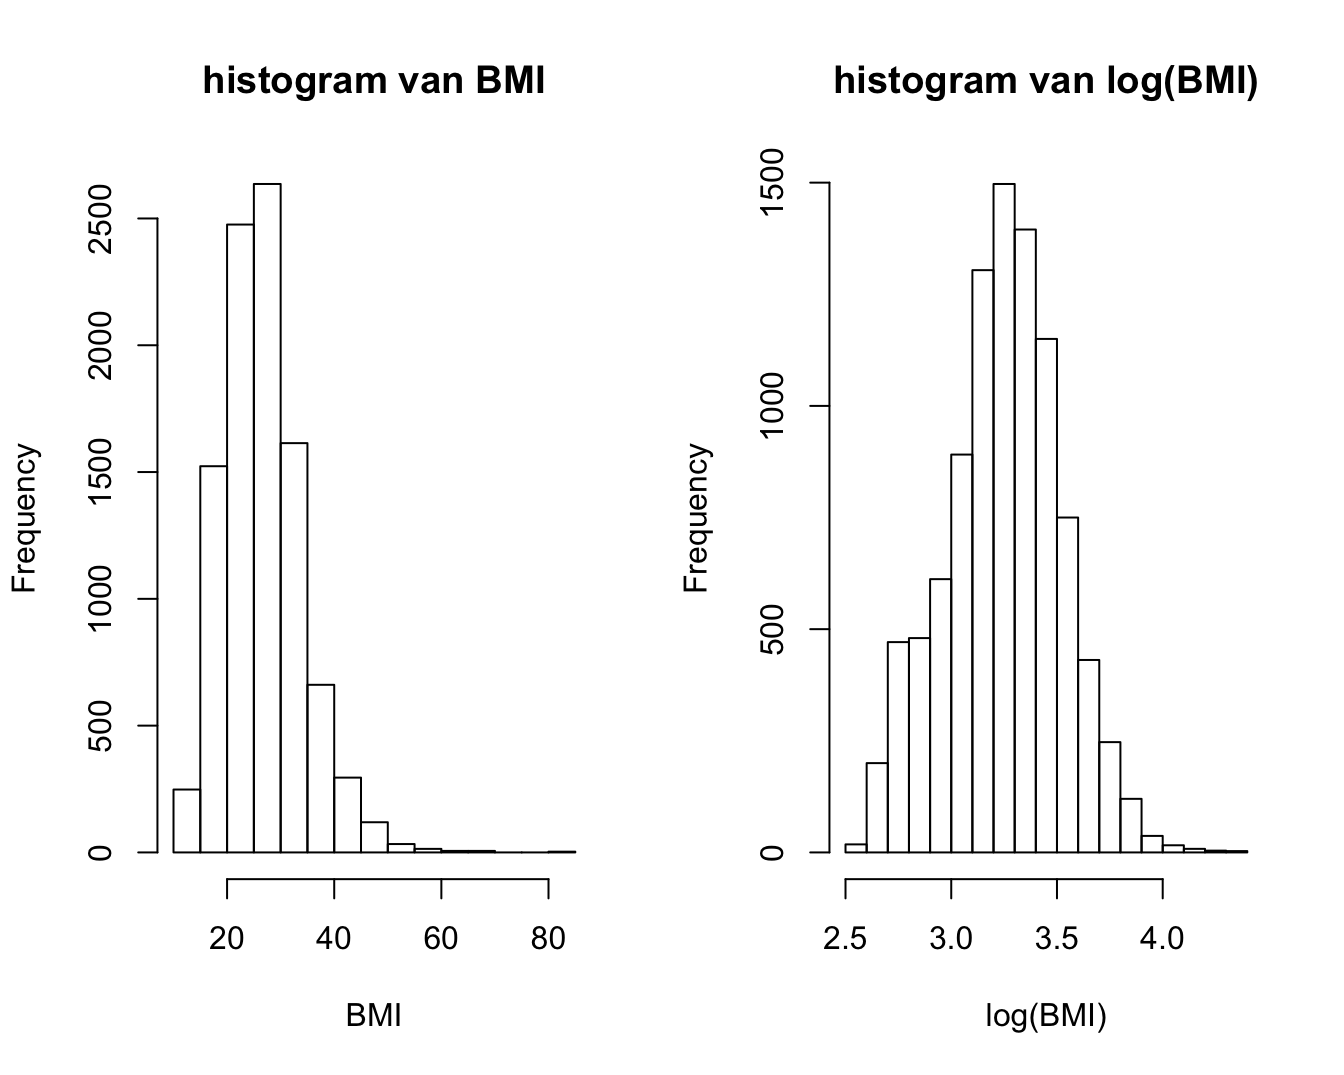
\includegraphics[width=1\linewidth]{Statistiek_2019_2020_files/figure-latex/histLogBMI-1} 

}

\caption{Boxplot van BMI en log(BMI) in de NHANES studie.}\label{fig:histLogBMI}
\end{figure}

In situaties waar de log-transformatie inderdaad de scheefheid wegneemt,
zal het geometrisch gemiddelde dichter bij de mediaan liggen dan het
gemiddelde. Wanneer de verdeling scheef is, is ze soms zelfs een
nuttigere maat voor centrale locatie dan de mediaan:

\begin{enumerate}
\def\labelenumi{\arabic{enumi}.}
\item
  omdat ze ook gebruik maakt van de exacte waarden van de observaties en
  daarom doorgaans preciezer is dan de mediaan;
\item
  omdat ze, op een transformatie na, berekend wordt als een rekenkundig
  gemiddelde (weliswaar van de logaritmisch getransformeerde
  observaties) en algemene statistische technieken voor een gemiddelde
  (zoals betrouwbaarheidsintervallen (zie volgende hoofdstukken) en
  toetsen van hypothesen (zie volgende hoofdstukken) daardoor vrijwel
  rechtstreeks toepasbaar zijn voor geometrische gemiddelden.
\end{enumerate}

\BeginKnitrBlock{example}[BMI]
\protect\hypertarget{exm:unnamed-chunk-44}{}{\label{exm:unnamed-chunk-44}
\iffalse (BMI) \fi{} }
\EndKnitrBlock{example} Het gemiddelde en mediane BMI bedraagt 26.66 en
25.98 , respectievelijk. Het gemiddelde is hier groter dan de mediaan
omdat de BMI scheef verdeeld is naar rechts (zie Figuur
\ref{fig:histLogBMI}). De verdeling wordt meer symmetrisch na
log-transformatie. Het gemiddelde en mediane log-BMI liggen ook dichter
bij elkaar en bedragen respectievelijk 3.25 en 3.26. De geometrisch
gemiddelde BMI-concentratie bekomen we door de exponentiële functie te
evalueren in 3.25, hetgeen ons 25.69 oplevert. Merk op dat dit inderdaad
beter met de mediaan overeenstemt dan het rekenkundig gemiddelde.

\texttt{**Einde\ voorbeeld**}

Tot slot, vooraleer een eenvoudige maat voor de centrale ligging (en
spreiding) te construeren of interpreteren, is het goed om altijd eerst
de volledige verdeling te bekijken! Immers, stel dat men het gemiddelde
of mediaan berekent van gegevens uit een bimodale verdeling (d.i. een
verdeling met 2 modi, voor bvb. zieken en niet-zieke dieren). Dan kan
het gemiddelde of mediaan makkelijk een zeer zeldzame waarde aannemen
die geenszins in de buurt van 1 van beide maxima ligt.

\subsection{Spreidingsmaten}\label{subsec:spreiding}

Nadat de centrale ligging van de gegevens werd bepaald, is men in tweede
instantie geïnteresseerd in de spreiding van de gegevens rond die
centrale waarde. Er zijn verschillende redenen waarom daar interesse in
bestaat:

\begin{enumerate}
\def\labelenumi{\arabic{enumi}.}
\tightlist
\item
  Om risico's te berekenen (zie Sectie \ref{sec:normal}) volstaat het
  niet om de centrale locatie van de gegevens te kennen, maar moet men
  bovendien weten hoeveel de gegevens rond die waarde variëren.
  Inderdaad, stel dat men wenst te weten welk percentage van de
  subjecten een BMI heeft van boven de 35. Wetende dat een geometrisch
  gemiddelde van 25.69 wordt geobserveerd, zal dat percentage relatief
  hoog zijn wanneer de metingen zeer gespreid zijn en relatief laag
  anders.
\item
  Veldbiologen zijn vaak geïnteresseerd in de mate waarin dieren of
  planten verspreid zijn over een zeker studiegebied. Op die manier
  kunnen ze immers leren over de relaties tussen individuen onderling en
  met hun omgeving. Daartoe zal men in de praktijk op verschillende
  plaatsen in het studiegebied tellingen maken van het aantal individuen
  op die plaats. Men kan aantonen dat, onder bepaalde
  veronderstellingen, individuen lukraak verspreid zijn over het
  studiegebied wanneer de spreiding op die tellingen, zoals gemeten door
  de variantie (zie verder), van dezelfde grootte-orde is als de
  gemiddelde telling. Indien de spreiding groter is, dan hebben
  individuen de neiging om zich te groeperen. Andersom, indien de
  spreiding op die tellingen lager is dan de gemiddelde telling, dan
  zijn de individuen zeer uniform verdeeld over het studiegebied.
\item
  Stel dat men een zekere uitkomst (bvb. het aantal species ongewervelde
  dieren in een stuk bodemkorst) wenst te vergelijken tussen 2 groepen
  (bvb. gebieden met en zonder bosbrand), dan zal men een duidelijk
  beeld van het groepseffect krijgen wanneer de uitkomst weinig gespreid
  is, maar een veel minder duidelijk beeld wanneer de gegevens meer
  chaotisch (en dus meer gespreid) zijn. Om uit te maken of een
  interventie-effect toevallig of systematisch is, moet men daarom een
  idee hebben van de spreiding op de gegevens.
\end{enumerate}

Dat uitkomsten variëren tussen individuen en binnen individuen omwille
van allerlei redenen ligt aan de basis van de statistische analyse van
veel fenomenen. Het goed beschrijven van variatie naast de centrale
locatie van de gegevens is daarom belangrijk! Hierbij zal men typisch
een onderscheid maken tussen variatie die men kan verklaren (door middel
van karakteristieken, zoals bijvoorbeeld de leeftijd, van de bestudeerde
individuen) en onverklaarde variatie. We gaan dieper in op dit
onderscheid in Hoofdstuk \ref{chap:linReg} rond lineaire regressie.

Variatie betekent dat niet alle observaties \(x_i\) gelijk zijn aan het
gemiddelde \(\overline{x}\). De afwijking \(x_i - \bar{x}\) is om die
reden interessant. Het gemiddelde van die afwijkingen is echter altijd 0
(verifieer!) omdat positieve en negatieve afwijkingen mekaar opheffen.
Bijgevolg levert de gemiddelde afwijking geen goede maat op voor de
variatie en is het beter om bijvoorbeeld naar kwadratische afwijkingen
\((x_i - \bar{x})^2\) te kijken. Het gemiddelde van die
\emph{kwadratische afwijkingen rond het gemiddelde}, het gemiddelde dus
van \((x_i - \bar{x})^2\), levert daarom wel een goede maat op. Merk op
dat we bij het berekenen van het gemiddelde niet delen door het aantal
observaties \(n\), maar door \(n-1\) waarbij we corrigeren voor het feit
dat we voor de berekening van de steekproef variantie 1 vrijheidsgraad
hebben gespendeerd aan het schatten van het gemiddelde.

\BeginKnitrBlock{definition}[variantie]
\protect\hypertarget{def:unnamed-chunk-45}{}{\label{def:unnamed-chunk-45}
\iffalse (variantie) \fi{} }De \textbf{variantie} een reeks waarnemingen
\(x_i, i=1, 2, \dots, n\) is per definitie

\begin{equation*}
s^2_x = \sum_{i=1}^{n} \frac{(x_i - \bar{x})^2}{n-1}
\end{equation*}

Als duidelijk is om welke waarnemingen het gaat, wordt dit ook met
\(s^2\) genoteerd.

\textbf{Einde definitie}
\EndKnitrBlock{definition}

Indien alle observaties gelijk waren en er dus geen variatie was, dan
zou hun variantie 0 bedragen. Hoe meer de gegevens uitgesmeerd zijn rond
hun gemiddelde, hoe groter \(s^2\). Helaas is de waarde van de variantie
zelf niet gemakkelijk te interpreteren. Dit is deels omdat door het
kwadrateren de variantie niet langer de dimensie van de oorspronkelijke
waarnemingen heeft. Handiger om mee te werken is daarom de
\emph{standaarddeviatie} of \emph{ standaardafwijking}:

\begin{equation*}
s_x= \sqrt{s_x^2} .
\end{equation*}

De standaarddeviatie is gedefinieerd voor elke numerieke variabele, maar
is vooral nuttig omdat voor heel wat variabelen (in het bijzonder
Normaal verdeelde variabelen - zie Sectie \ref{sec:normal}) bij
benadering 68\% van de waarnemingen liggen tussen \(\bar{x} - s_x\) en
\(\bar{x} + s_x\), en 95\% van de waarnemingen liggen tussen\footnote{Later
  zullen we zien dat het nog iets correcter is om te stellen dat 95\%
  van de waarnemingen liggen tussen \(\bar{x} - 1.96 s_x\) en
  \(\bar{x} + 1.96 s_x\).} \(\bar{x} - 2 s_x\) en \(\bar{x} + 2 s_x\).
Deze intervallen noemt men respectievelijk 68\% en 95\%
\emph{referentie-intervallen}. Het is precies deze eigenschap die de
standaarddeviatie zo nuttig maakt in de praktijk. De standaarddeviatie
van een reeks waarnemingen wordt vaak afgekort als SD in de
wetenschappelijke literatuur.

\textbf{Eigenschap}

Als alle uitkomsten \(x_i\) met een willekeurige constante \(a\) worden
vermenigvuldigd, dan wordt hun variantie vermenigvuldigd met \(a^2\) en
hun standaarddeviatie met \(|a|\) (de absolute waarde van \(a\)). Als
bij alle uitkomsten \(a\) wordt opgeteld, wijzigen hun variantie en
standaarddeviatie niet.

\textbf{Einde eigenschap}

\begin{Shaded}
\begin{Highlighting}[]
\CommentTok{# Het gebruik van functie sd() levert de}
\CommentTok{# standarddeviatie van de variabele BMI in de}
\CommentTok{# NHANES dataset.  Het na.rm=TRUE argument wordt}
\CommentTok{# gebruikt omdat er ontbrekende waarnemingen}
\CommentTok{# voorkomen.}
\KeywordTok{sd}\NormalTok{(NHANES}\OperatorTok{$}\NormalTok{BMI, }\DataTypeTok{na.rm =} \OtherTok{TRUE}\NormalTok{)}
\end{Highlighting}
\end{Shaded}

\begin{verbatim}
## [1] 7.376579
\end{verbatim}

\begin{Shaded}
\begin{Highlighting}[]
\CommentTok{# levert de variantie van de variabele BMI}
\KeywordTok{var}\NormalTok{(NHANES}\OperatorTok{$}\NormalTok{BMI, }\DataTypeTok{na.rm =} \OtherTok{TRUE}\NormalTok{)}
\end{Highlighting}
\end{Shaded}

\begin{verbatim}
## [1] 54.41392
\end{verbatim}

Wanneer een variabele niet Normaal verdeeld is (dit is bijvoorbeeld het
geval voor het BMI gezien het niet symmetrisch verdeeld is), dan geldt
niet langer dat bij benadering 95\% van de waarnemingen ligt tussen
\(\bar{x} - 2 s\) en \(\bar{x} + 2 s\). Een symmetrische maat voor de
spreiding van de gegevens, zoals de standaarddeviatie, is dan niet
langer interessant. In dat geval zijn de range en interkwantielafstand
betere maten.

\BeginKnitrBlock{definition}[bereik en interkwartielafstand]
\protect\hypertarget{def:unnamed-chunk-47}{}{\label{def:unnamed-chunk-47}
\iffalse (bereik en interkwartielafstand) \fi{} }Het \textbf{bereik} of
de \textbf{range} \(R_x\) van een reeks waarnemingen
\(x_i, i=1,2,...,n\), is per definitie het verschil tussen de grootste
en kleinste geobserveerde waarde. De \textbf{interkwartielafstand} van
een reeks waarnemingen \(x_i, i=1,2,...,n\) is per definitie de afstand
tussen het derde kwartiel \(x_{75}\) en het eerste kwartiel \(x_{25}\).
Dat wordt ook grafisch weergegeven op een boxplot (breedte van de box).
Hierbinnen liggen circa 50\% van de observaties. Circa 95\% van de
observaties kan men vinden tussen het 2.5\% en 97.5\% percentiel.

\textbf{Einde definitie}
\EndKnitrBlock{definition}

Het bereik is zeer gevoelig voor outliers en is systematisch afhankelijk
van het aantal observaties: hoe groter \(n,\) hoe groter men \(R_x\)
verwacht. Om die reden vormt een interkwartielafstand een betere maat
voor de spreiding van de gegevens dan de range.

Tenslotte is het vaak zo dat de gegevens meer gespreid zijn naarmate hun
gemiddelde hogere waarden aanneemt. De
\emph{variatiecoëfficiënt}=\(VC_x\) standaardiseert daarom de
standaarddeviatie door ze uit te drukken als een percentage van het
gemiddelde

\begin{equation*}
VC_x = \frac{s_x}{\bar{x}} 100\%.
\end{equation*}

Omdat ze gestandaardiseerd is, dient ze beter dan de standaarddeviatie
zelf om de spreiding op de gegevens te vergelijken tussen populaties met
een verschillend gemiddelde. De variatiecoëfficiënt heeft verder de
aantrekkelijke eigenschap dat ze geen eenheden heeft en ongevoelig is
voor herschaling van de gegevens (d.w.z. wanneer alle gegevens met een
constante \(a\) worden vermenigvuldigd, dan is \(VC_{ax}=VC_x\)).

\section{De Normale benadering van gegevens}\label{sec:normal}

Bij biologische en chemische data is het vaak zo dat het histogram van
een continue meting bij verschillende subjecten de karakteristieke vorm
heeft van de Normale verdeling, die geïllustreerd wordt in Figuur
\ref{fig:continu} (linksboven). Dat is bijvoorbeeld zo als men een
histogram maakt van het logaritme van de totale cholestorol. Rond 1870
opperde de wereldberoemde Belg Adolphe Quetelet (die tevens de eerste
student was die een doctoraat behaalde aan de Universiteit Gent) de idee
om deze curve als `ideaal histogram' te gebruiken voor de voorstelling
en vergelijking van gegevens. Dit zal handig blijken om meer inzicht te
krijgen in de gegevens op basis van een minimum aantal
samenvattingsvatten, zoals het gemiddelde en de standaarddeviatie die
vaak in wetenschappelijke rapporten vermeld staan.

\begin{figure}

{\centering 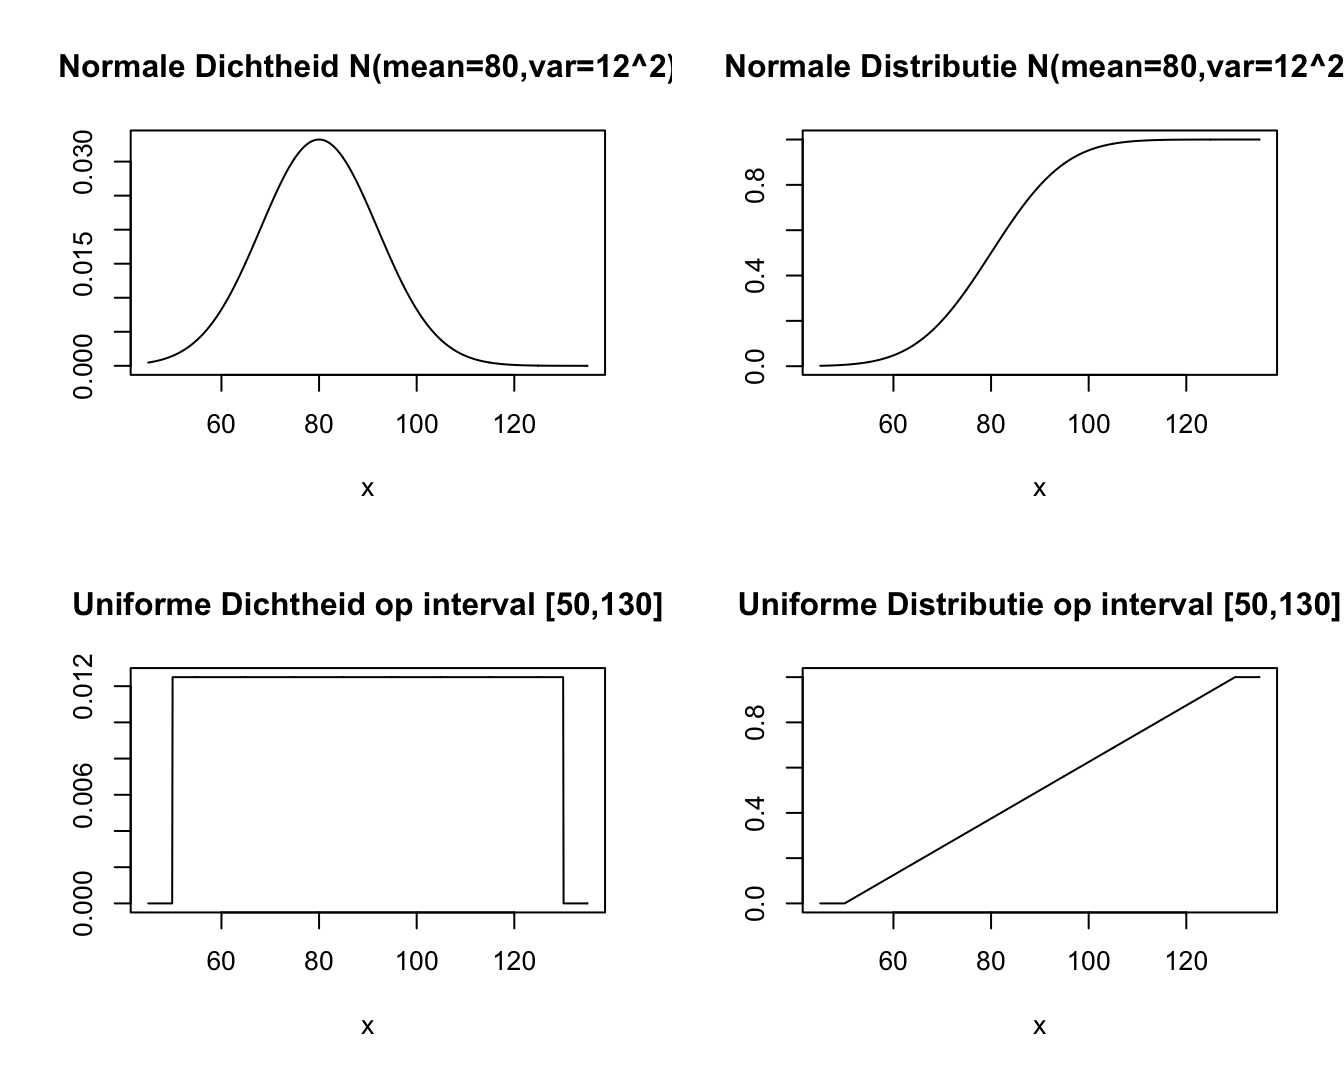
\includegraphics[width=1\linewidth]{Statistiek_2019_2020_files/figure-latex/continu-1} 

}

\caption{De Normale dichtheidsfunctie (boven, links), de Normale distributiefunctie (boven, rechts), de Uniforme dichtheidsfunctie (onder, links) en de Uniforme distributiefunctie (onder, rechts).}\label{fig:continu}
\end{figure}

\subsection{Bepalen van oppervlaktes onder de Normale
curve}\label{subsec:normalcalc}

De \emph{Normale curve} of \emph{Normale dichtheidsfunctie} wordt
gegeven door:

\begin{equation*}
f(x) = \frac{1}{\sigma \sqrt{2 \pi} } \exp \left ( - \frac{ (x - \mu)^2 }{ 2
\sigma^2} \right ).
\end{equation*}

Ze wordt beschreven door 2 onbekende parameters \(\mu\) en \(\sigma\),
waarbij \(\mu\) het gemiddelde van de verdeling van de observaties
aangeeft en \(\sigma\) de standaarddeviatie. Deze curve geeft voor elke
waarde \(x\) weer hoe frequent deze waarde, relatief gezien, voorkomt.
De notatie \(\pi\) verwijst naar het getal \(\pi=3.1459...\) Wanneer het
gemiddelde 0 is en de variantie 1, spreekt men van de
\emph{standaardnormale curve} of \emph{standaardnormale
dichtheidsfunctie}.

Een lukrake observatie uit een reeks gegevens wiens verdeling de Normale
curve volgt, wordt een \textbf{Normaal verdeelde observatie} genoemd.
Dergelijke observaties komen frequent voor: voor heel wat reeksen
gegevens die symmetrisch verdeeld zijn, vormt de Normale curve met
\(\mu\) gelijk aan \(\bar x\) en \(\sigma\) gelijk aan \(s_x\) immers
een goede benadering voor het histogram.

Voor Normaal verdeelde gegevens geeft de oppervlakte onder de Normale
curve tussen 2 willekeurige getallen \(a\) en \(b\) het percentage van
de observaties weer dat tussen deze 2 getallen gelegen is. Op die manier
laat de Normale curve toe om, enkel op basis van kennis van het
gemiddelde en de standaarddeviatie, na te gaan welk percentage van de
gegevens bij benadering tussen 2 willekeurige getallen \(a\) en \(b\)
gelegen is.

Om deze berekening uit te voeren, gaan we als volgt te werk. Zij \(X\)
een lukrake meting uit een reeks Normaal verdeelde gegevens met
gemiddelde \(\mu\) en standaarddeviatie \(\sigma\). Dan noteren we met
\(P(X\leq b)\) de oppervlakte onder de Normale curve die links van \(b\)
gelegen is, en met \(P(a\leq X\leq b)\) de oppervlakte onder de Normale
curve tussen \(a\) en \(b\). Hierbij is\footnote{Hierbij maken we
  gebruik van het feit dat voor een Normaal verdeelde observatie \(X\),
  \(P(X=a)=0\) voor elk reëel getal \(a\), zodat \(P(X\leq a)=P(X<a)\).}

\begin{equation*}
P(a\leq X\leq b)=P(X\leq b)-P(X\leq a)
\end{equation*}

Om \(P(a\leq X\leq b)\) te berekenen, hebben we dus enkel een strategie
nodig om voor een willekeurig getal \(x\), het getal
\(F(x) = P(X \leq x)\) uit te rekenen. Dit staat uitgezet in functie van
\(x\) in Figuur \ref{fig:continu} (rechtsboven) voor \(\mu=80\) en
\(\sigma=12\) en wordt een \emph{distributiefunctie} genoemd.

\BeginKnitrBlock{definition}[distributiefunctie]
\protect\hypertarget{def:unnamed-chunk-48}{}{\label{def:unnamed-chunk-48}
\iffalse (distributiefunctie) \fi{} }De functie die voor elk getal \(x\)
uitdrukt wat de kans is dat een lukrake meting \(X\) met gekende
verdeling (bvb. een Normale verdeling) kleiner of gelijk is aan \(x\),
wordt de \textbf{distributiefunctie} van die verdeling genoemd.

\textbf{Einde definitie}
\EndKnitrBlock{definition}

Omdat de Normale dichtheidsfunctie zeer complex is, blijkt dat het getal
\(F(x)\) niet expliciet uit te rekenen is. Om die reden heeft men de
getallen \(F(x)\) voor de standaardnormale verdelingsfunctie
getabuleerd. Voor deze standaardnormale curve duidt men voor een
willekeurige waarde \(z\), het getal \(F(z)\) met \(\Phi(z)\) aan.
Omwille van de symmetrie rond 0 van de standaardnormale curve kan de
waarde van \(\Phi(-z)\) dan uit de waarde van \(\Phi(z)\) worden
afgeleid als

\begin{equation*}
\Phi(-z)= 1- \Phi(z)
\end{equation*}

Deze uitdrukking geeft aan dat voor een reeks standaardnormaal verdeelde
metingen, het percentage dat kleiner is dan \(-z\) gelijk is aan het
percentage dat groter is dan \(z\).

Om nu \(P(a\leq X\leq b)\) te berekenen op basis van de tabellen voor de
standaardnormale verdeling gaan we als volgt te werk. Vooreerst kan men
aantonen dat het resultaat van een lineaire transformatie \(aX+b\) op
een Normaal verdeelde meting \(X\) met gemiddelde \(\mu\) en
standaarddeviatie \(\sigma\) terug een Normaal verdeelde meting
toevalsveranderlijke is, maar nu met gemiddelde \(a\mu+b\) en
standaarddeviatie \(|a|\sigma\). Op die manier kan men elke Normaal
verdeelde meting met gemiddelde \(\mu\) en standaarddeviatie \(\sigma\)
omzetten naar een standaardnormale meting door ze als volgt te
\emph{standaardiseren}:

\begin{equation*}
Z = \frac{X- \mu}{\sigma}
\end{equation*}

Verifieer dat \(Z\) inderdaad gemiddelde 0 en standaarddeviatie 1 heeft!

Aangezien voor een willekeurig getal \(x\)

\begin{equation*}
X\leq x \Leftrightarrow \frac{X-\mu}{\sigma} \leq \frac{x-\mu}{\sigma}
\end{equation*}

vinden we nu dat

\begin{eqnarray*}
P(a \leq X \leq b) & = & P\left(\frac{a-\mu}{\sigma} \leq Z \leq \frac{b-\mu%
}{\sigma} \right) \\
& = & \Phi \left (\frac{b-\mu}{\sigma} \right ) - \Phi \left (\frac{a-\mu}{%
\sigma} \right )
\end{eqnarray*}

De getallen \(\Phi \left (\frac{b-\mu}{\sigma} \right )\) en
\(\Phi \left (\frac{a-\mu}{\sigma} \right )\) kunnen hierbij
rechtstreeks uit tabellen of R software worden gehaald. In het vervolg
zullen we algemeen de notatie \(Z\) gebruiken om een standaardnormaal
verdeelde meting aan te duiden.

\BeginKnitrBlock{exercise}
\protect\hypertarget{exr:unnamed-chunk-49}{}{\label{exr:unnamed-chunk-49} }
\EndKnitrBlock{exercise} Een labo bepaalt in een visstaal Hg via een
methode op basis van AAS. In werkelijkheid bevat het staal (gemiddeld)
1.90 ppm. De meetmethode is echter niet perfect, zoals aangegeven door
een standaarddeviatie van 0.10 ppm. Wat is de kans dat de laborant die
het staal onderzoekt, een meetresultaat van 2.10 ppm of meer vaststelt?

Om op deze vraag te antwoorden, noteren we met \(X\) het meetresultaat
van de laborant en berekenen we

\begin{eqnarray*}
P(X\geq 2)&=&P\left(\frac{X-\mu}{\sigma}\geq \frac{2.1-1.9}{0.1}\right) \\
&=&P(Z\geq 2) = 2.28\%
\end{eqnarray*}

We besluiten dat er 2.28\% kans is dat de laborant een meetresultaat van
minstens 2.10 ppm zal vaststellen. In R kan dit resultaat als volgt
bekomen worden:

\begin{Shaded}
\begin{Highlighting}[]
\DecValTok{1} \OperatorTok{-}\StringTok{ }\KeywordTok{pnorm}\NormalTok{(}\FloatTok{2.1}\NormalTok{, }\DataTypeTok{mean =} \FloatTok{1.9}\NormalTok{, }\DataTypeTok{sd =} \FloatTok{0.1}\NormalTok{)}
\end{Highlighting}
\end{Shaded}

\begin{verbatim}
## [1] 0.02275013
\end{verbatim}

waarbij de functie pnorm de distributiefunctie van de Normale verdeling
voorstelt.

\texttt{**Einde\ oefening**}

Met \(z_{\alpha}\) duiden\footnote{Let wel op want in verschillende
  boeken krijgt het symbool \(z_{\alpha}\) verschillende definities!} we
die waarde aan waar \(\alpha100\%\) van de oppervlakte onder de
standaardnormale curve rechts van zit; m.a.w. waarvoor geldt dat
\(P(Z \geq z_{\alpha}) = \alpha\). Als \(Z\) een standaardnormaal
verdeelde meting is, dan stelt \(z_{\alpha}\) bijgevolg het
\((1-\alpha)100\%\) percentiel van die verdeling voor. Voor
\(z_{\alpha/2}\) geldt dat
\(P(-z_{\alpha/2}\leq Z \leq z_{\alpha/2}) = 1-\alpha\). Bijvoorbeeld,
\(P( - z_{0.025}\leq Z \leq z_{0.025}) = 95\%\). Voor een reeks
standaardnormaal verdeelde metingen bevat het interval
\([-z_{\alpha/2},z_{\alpha/2}]\) dus \((1-\alpha)100\%\) van de
observaties.

Stel dat \(X\) een Normaal verdeelde meting is met gemiddelde \(\mu\) en
standaarddeviatie \(\sigma\). Dan geldt dat

\begin{equation*}
P\left( - z_{\alpha/2}\leq \frac{X - \mu}{\sigma} \leq z_{\alpha/2}\right) =
1-\alpha .
\end{equation*}

Hieruit volgt dat

\begin{equation*}
P( \mu - z_{\alpha/2} \sigma \leq X \leq \mu + z_{\alpha/2} \sigma ) =
1-\alpha .
\end{equation*}

Voor een reeks Normaal verdeelde metingen met gemiddelde \(\mu\) en
standaarddeviatie \(\sigma\) bevat het interval
\([\mu-z_{\alpha/2}\sigma,\mu+z_{\alpha/2}\sigma]\) dus
\((1-\alpha)100\%\) van de observaties. In de praktijk worden de
parameters \(\mu\) en \(\sigma\) hierbij vervangen door \(\bar x\) en
\(s_x\).

Het resulterende interval
\([\bar x-z_{\alpha/2}s_x,\bar x+z_{\alpha/2}s_x]\) wordt vaak
gebruikt\footnote{Dit interval bevat niet exact \((1-\alpha)100\%\) van
  de observaties, maar slechts bij benadering, omdat het geen rekening
  houdt met het feit dat \(\bar x\) en \(\sigma_x\) impreciese
  schattingen zijn voor \(\mu\) en \(\sigma\) op basis van een eindige
  steekproef. Meer accurate referentie-intervallen die deze imprecisie
  in rekening brengen, ook predictie-intervallen genoemd}, o.a. in de
klinische chemie, om \emph{referentie-intervallen} te berekenen voor een
test ter opsporing van een bepaalde pathologie. Eenmaal zo'n
referentie-interval, ook wel \emph{normaal interval} genoemd, werd
bepaald, wordt het testresultaat van een patiënt met de vermoede
pathologie vergeleken met het interval. Een resultaat buiten het
interval is dan indicatief voor de aanwezigheid van de pathologie.

Bij het bepalen van referentie-intervallen is het noodzakelijk om de
methode eerst te testen bij mensen zonder de pathologie in kwestie. Voor
dit doel worden `normale en gezonde vrijwilligers' aangezocht. Vaak
worden hiertoe collega's genomen uit het laboratorium dat de test heeft
ontwikkeld, hoewel dit allesbehalve ideaal is. Immers, mensen die in een
zelfde laboratorium werken, zijn blootgesteld aan dezelfde werkomgeving,
die op zijn beurt een invloed kan hebben op hun bloedsamenstelling.
Bijgevolg is de bloedsamenstelling van de studiepersonen mogelijks niet
representatief voor een normale, gezonde populatie, hetgeen kan leiden
tot vertekende referentie-intervallen. In deze cursus zullen we een
referentie-interval meer algemeen als volgt definiëren.

\BeginKnitrBlock{definition}[referentie-interval]
\protect\hypertarget{def:unnamed-chunk-51}{}{\label{def:unnamed-chunk-51}
\iffalse (referentie-interval) \fi{} }Een \textbf{\((1-\alpha)100\%\)
referentie-interval} voor een veranderlijke \(X\) (bvb.
albumine-concentratie in het bloed) in een gegeven studiepopulatie (bvb.
volwassen Belgen onder de 60 jaar) is een interval dat zó gekozen werd
dat het met \((1-\alpha)100\%\) kans de observatie voor een lukraak
individu uit die populatie bevat. Voor een Normaal verdeelde
veranderlijke \(X\) met gemiddelde \(\mu\) en standaarddeviatie
\(\sigma\) kan dit berekend worden als

\begin{equation*}
[\mu-z_{\alpha/2}\sigma,\mu+z_{\alpha/2}\sigma]
\end{equation*}

en geschat worden op basis van een lukrake steekproef als

\begin{equation*}
[\bar x-z_{\alpha/2}s_x,\bar x+z_{\alpha/2}s_x]
\end{equation*}

\textbf{Einde definitie}
\EndKnitrBlock{definition}

\BeginKnitrBlock{example}[Referentie-intervallen]
\protect\hypertarget{exm:unnamed-chunk-52}{}{\label{exm:unnamed-chunk-52}
\iffalse (Referentie-intervallen) \fi{} }
\EndKnitrBlock{example} In het Hoofdstuk \ref{chap:besluit} statistische
besluitvorming handelt de centrale dataset rond een studie naar het
effect van het toedienen van een bloeddrukverlagend middel captopril.
Alvorens de studie aan te vangen dient men eerst een grenswaarde voor
normale bloeddrukwaarden op te stellen om subjecten met normale
bloeddrukken van patiënten met hypertensie te kunnen onderscheiden. We
zullen hiervoor gebruik maken van een subset van de NHANES studie. In
Figuur \ref{fig:sysBp} links wordt een histogram gegeven van alle
bloeddruk waarden voor subjecten tussen de 40 en 65 jaar. Rechts wordt
het histogram weergegeven voor gezonde subjecten tussen de 40 en 65
jaar, waarbij gezonde personen werden geselecteerd op basis van hun BMI
klasse, rokers, status algemene gezondheidsstatus, slaapproblemen, of ze
aan diabetes lijden en ze in het verleden hard drugs gebruikten.

\begin{Shaded}
\begin{Highlighting}[]
\CommentTok{# verwijderen van alle subjecten met ontbrekende}
\CommentTok{# waarnemingen}
\NormalTok{NHANES2 =}\StringTok{ }\KeywordTok{subset}\NormalTok{(NHANES, }\OperatorTok{!}\KeywordTok{is.na}\NormalTok{(Race1) }\OperatorTok{&}\StringTok{ }\OperatorTok{!}\KeywordTok{is.na}\NormalTok{(Smoke100n) }\OperatorTok{&}\StringTok{ }
\StringTok{    }\OperatorTok{!}\KeywordTok{is.na}\NormalTok{(BMI_WHO) }\OperatorTok\StringTok{ }\OperatorTok{!}\KeywordTok{is.na}\NormalTok{(Age) }\OperatorTok{&}\StringTok{ }\OperatorTok{!}\KeywordTok{is.na}\NormalTok{(HardDrugs) }\OperatorTok{&}\StringTok{ }
\StringTok{    }\OperatorTok{!}\KeywordTok{is.na}\NormalTok{(HealthGen) }\OperatorTok{&}\StringTok{ }\OperatorTok{!}\KeywordTok{is.na}\NormalTok{(Gender) }\OperatorTok{&}\StringTok{ }\OperatorTok{!}\KeywordTok{is.na}\NormalTok{(AlcoholYear) }\OperatorTok{&}\StringTok{ }
\StringTok{    }\OperatorTok{!}\KeywordTok{is.na}\NormalTok{(BPSys1) }\OperatorTok{&}\StringTok{ }\OperatorTok{!}\KeywordTok{is.na}\NormalTok{(BPSys2) }\OperatorTok{&}\StringTok{ }\OperatorTok{!}\KeywordTok{is.na}\NormalTok{(BPSys3) }\OperatorTok{&}\StringTok{ }
\StringTok{    }\OperatorTok{!}\KeywordTok{is.na}\NormalTok{(SleepTrouble))}
\NormalTok{NHANES2}\OperatorTok{$}\NormalTok{bpSys =}\StringTok{ }\KeywordTok{rowMeans}\NormalTok{(NHANES2[, }\KeywordTok{c}\NormalTok{(}\DecValTok{27}\NormalTok{, }\DecValTok{29}\NormalTok{, }\DecValTok{31}\NormalTok{)])}
\CommentTok{# subset van de personen tussen 40 en 65 jaar}
\NormalTok{nhanesSub =}\StringTok{ }\KeywordTok{subset}\NormalTok{(NHANES2, Age }\OperatorTok{<=}\StringTok{ }\DecValTok{65} \OperatorTok{&}\StringTok{ }\NormalTok{Age }\OperatorTok{>=}\StringTok{ }\DecValTok{40} \OperatorTok{&}\StringTok{ }
\StringTok{    }\OperatorTok{!}\KeywordTok{duplicated}\NormalTok{(ID))}
\CommentTok{# De == operator resulteert in een bolean (FALSE of}
\CommentTok{# TRUE) de & operater is een logische AND}

\CommentTok{# subset van gezonde personen}
\NormalTok{nhanesSubHealthy =}\StringTok{ }\KeywordTok{subset}\NormalTok{(nhanesSub, Smoke100n }\OperatorTok{==}\StringTok{ "Non-Smoker"} \OperatorTok{&}\StringTok{ }
\StringTok{    }\NormalTok{Diabetes }\OperatorTok{==}\StringTok{ "No"} \OperatorTok{&}\StringTok{ }\KeywordTok{as.double}\NormalTok{(BMI_WHO) }\OperatorTok\StringTok{ }\KeywordTok{c}\NormalTok{(}\DecValTok{2}\NormalTok{, }
    \DecValTok{3}\NormalTok{) }\OperatorTok{&}\StringTok{ }\NormalTok{HardDrugs }\OperatorTok{==}\StringTok{ "No"} \OperatorTok{&}\StringTok{ }\NormalTok{HealthGen }\OperatorTok{!=}\StringTok{ "Poor"} \OperatorTok{&}\StringTok{ }
\StringTok{    }\NormalTok{SleepTrouble }\OperatorTok{==}\StringTok{ "No"}\NormalTok{)}
\KeywordTok{par}\NormalTok{(}\DataTypeTok{mfrow =} \KeywordTok{c}\NormalTok{(}\DecValTok{1}\NormalTok{, }\DecValTok{2}\NormalTok{))}
\KeywordTok{hist}\NormalTok{(nhanesSub}\OperatorTok{$}\NormalTok{bpSys, }\DataTypeTok{xlab =} \StringTok{"Systolische bloeddruk (mm Hg)"}\NormalTok{, }
    \DataTypeTok{main =} \StringTok{"Personen tussen 40-65 jaar"}\NormalTok{)}
\KeywordTok{hist}\NormalTok{(nhanesSubHealthy}\OperatorTok{$}\NormalTok{bpSys, }\DataTypeTok{xlab =} \StringTok{"Systolische bloeddruk (mm Hg)"}\NormalTok{, }
    \DataTypeTok{main =} \StringTok{"Gezonde personen tussen 40-65 jaar"}\NormalTok{)}
\end{Highlighting}
\end{Shaded}

\begin{figure}

{\centering 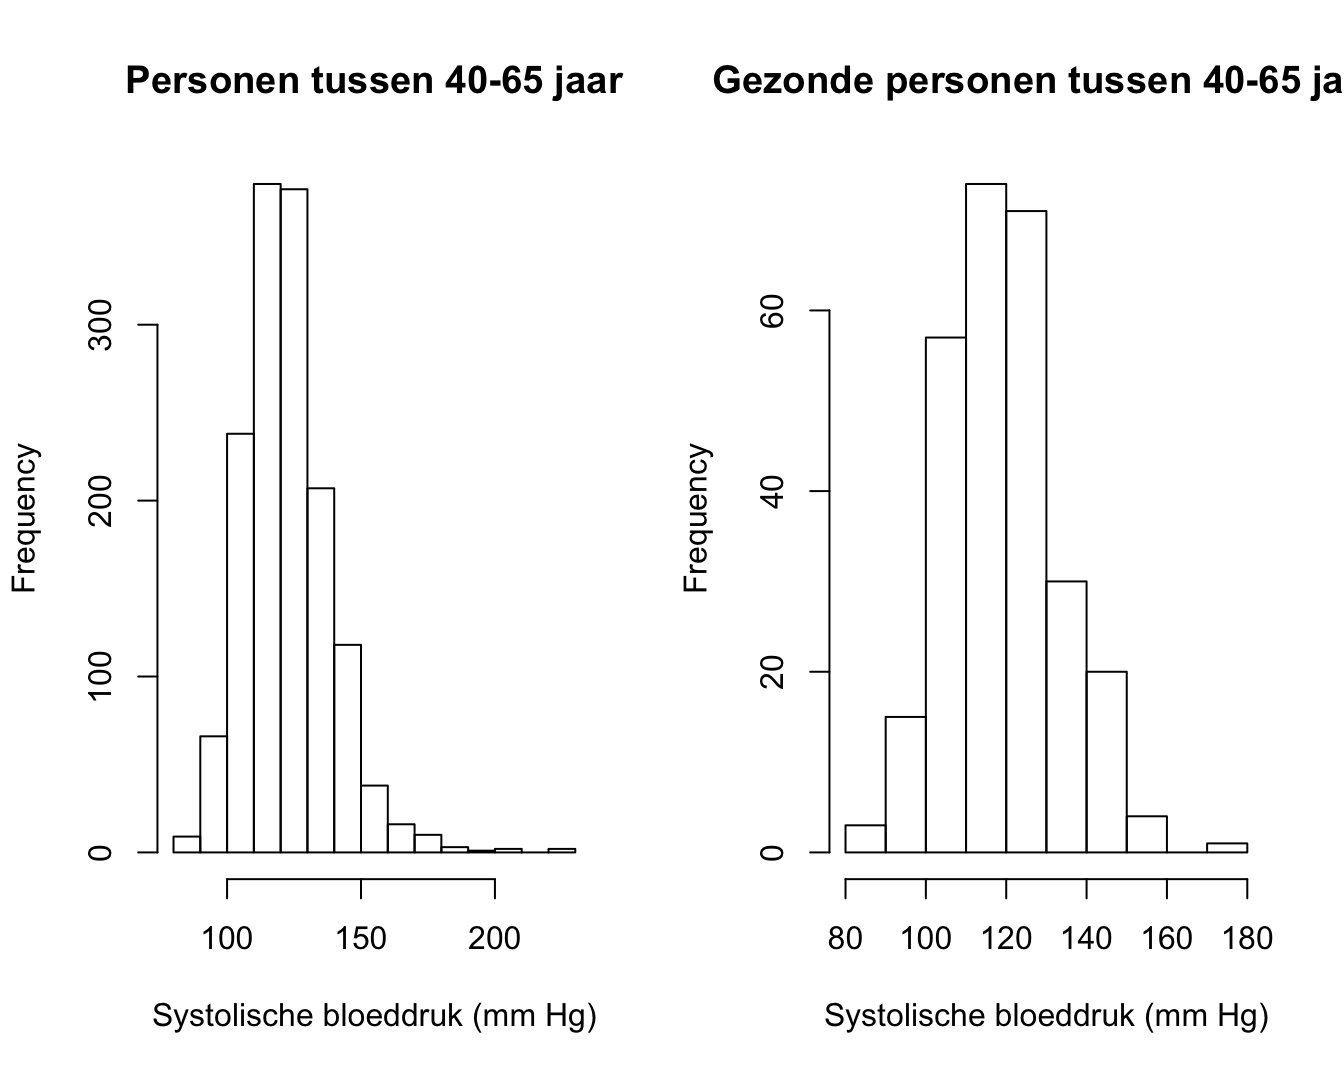
\includegraphics[width=1\linewidth]{Statistiek_2019_2020_files/figure-latex/sysBp-1} 

}

\caption{Systolische bloeddruk bij personen tussen de 40 en 65 jaar oud.}\label{fig:sysBp}
\end{figure}

De systolische bloeddruk voor gezonde personen is symmetrisch en we
zullen later aantonen dat deze approximatief normaal verdeeld zijn. Als
het gemiddelde en de standard deviatie van de bloeddruk in de populatie
gekend zijn kunnen we normale bloeddrukwaarden afleiden. In de praktijk
zijn deze typisch niet gekend en worden deze geschat op basis van de
data. In de gezonde subset is het steekproefgemiddelde 119.5mmHg en de
standaarddeviatie 14.1mmHg. Als we het populatiegemiddelde en het
populatiestandaarddeviatie door deze schattingen vervangen dan bekomen
we volgend referentie interval: {[}91.9, 147{]}mmHg.

Merk ook op dat de bovengrens van de normale systolische bloeddruk iets
boven de grens van hypertensie van 140 mmHg ligt die in de literatuur
wordt gehanteerd.

\texttt{**Einde\ voorbeeld**}

\begin{Shaded}
\begin{Highlighting}[]
\KeywordTok{mean}\NormalTok{(nhanesSubHealthy}\OperatorTok{$}\NormalTok{bpSys) }\OperatorTok{+}\StringTok{ }\KeywordTok{qnorm}\NormalTok{(}\KeywordTok{c}\NormalTok{(}\FloatTok{0.025}\NormalTok{, }\FloatTok{0.975}\NormalTok{)) }\OperatorTok{*}\StringTok{ }
\StringTok{    }\KeywordTok{sd}\NormalTok{(nhanesSubHealthy}\OperatorTok{$}\NormalTok{bpSys)}
\end{Highlighting}
\end{Shaded}

\begin{verbatim}
## [1]  91.88971 147.03393
\end{verbatim}

\subsection{QQ-plots}\label{sec:qq}

Hoewel heel wat metingen in de biologische wetenschappen en scheikunde,
zoals concentraties van een bepaalde stof, scheef verdeeld zijn naar
rechts, worden ze door het nemen van een logaritme vaak getransformeerd
naar gegevens waarvoor het histogram de vorm heeft van een Normale
dichtheidsfunctie. Dit is uiteraard niet altijd zo en stappen om te
verifiëren of observaties Normaal verdeeld zijn, zijn daarom van groot
belang om de technieken in Sectie \ref{subsec:normalcalc} te kunnen
gebruiken, alsook heel wat technieken uit de verdere hoofdstukken die er
zullen van uit gaan dat de gegevens Normaal verdeeld zijn. Hoewel een
vergelijking van het histogram van de gegevens met de vorm van de
Normale curve wel inzicht geeft of de gegevens al dan niet Normaal
verdeeld zijn, is dit vaak niet makkelijk te zien en wordt de
uiteindelijke beslissing nogal makkelijk beïnvloed door de keuze van de
klassebreedtes op het histogram. Om die reden zullen we
kwantielgrafieken gebruiken die duidelijker toelaten om na te gaan of
gegevens Normaal verdeeld zijn.

\emph{QQ-plots} of \emph{kwantielgrafieken} (in het Engels:
\emph{quantile-quantile plots}) zijn grafieken die toelaten te
verifiëren of een reeks observaties lukrake trekkingen zijn uit een
Normale verdeling. Met andere woorden, ze laten toe om na te gaan of een
reeks observaties al dan niet de onderstelling tegenspreken dat ze
realisaties zijn van een reeks Normaal verdeelde gegevens. Het principe
achter deze grafieken is vrij eenvoudig. Verschillende percentielen die
men heeft berekend voor de gegeven reeks observaties worden uitgezet
t.o.v. de overeenkomstige percentielen die men verwacht op basis van de
Normale curve. Als de onderstelling correct is dat de gegevens Normaal
verdeeld zijn, dan komen beide percentielen telkens vrij goed met elkaar
overeen en verwacht men bijgevolg een reeks puntjes min of meer op een
rechte te zien (zoals in Figuur \ref{fig:qq}, rechtsboven).
Systematische afwijkingen van een rechte wijzen op systematische
afwijkingen van Normaliteit. Lukrake afwijkingen van een rechte kunnen
het gevolg zijn van toevallige biologische variatie en zijn daarom niet
indicatief voor afwijkingen van Normaliteit. We gebruiken hiervoor de
functie \texttt{qqPlot} uit het package \texttt{car}. De qqPlot functie
geeft op de figuur ook banden weer waarbinnen punten uit de normaal
verdeling met een kans van 95\% kunnen worden verwacht.

\begin{verbatim}
## [1]  60 235
\end{verbatim}

\begin{figure}

{\centering 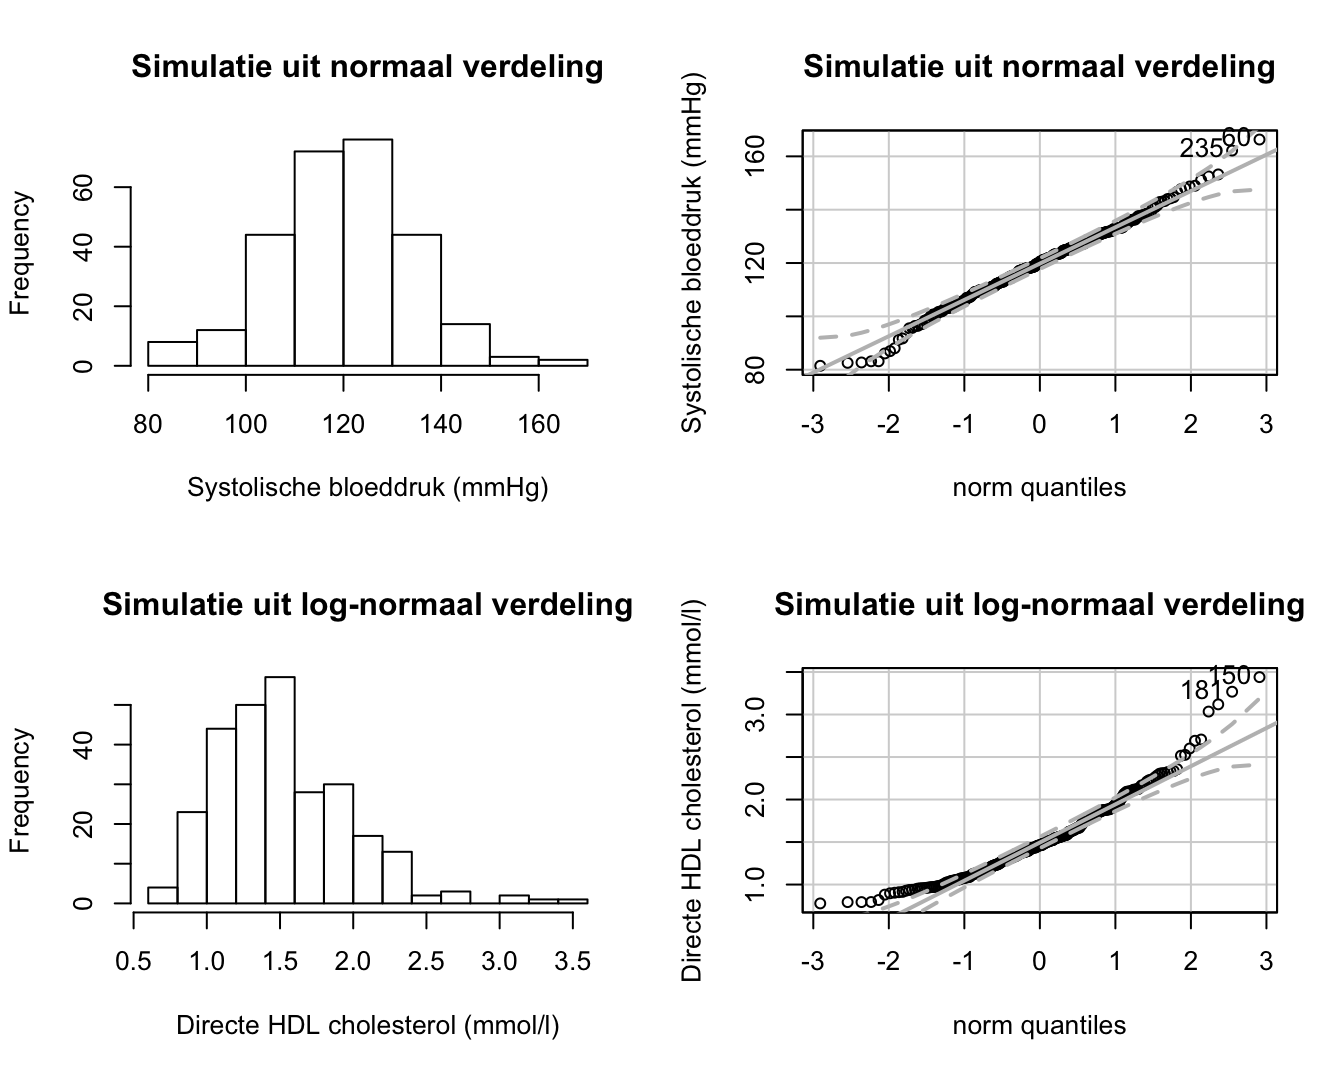
\includegraphics[width=1\linewidth]{Statistiek_2019_2020_files/figure-latex/qq-1} 

}

\caption{Histogrammen (links) en bijhorende kwantielgrafieken (rechts) voor een aantal verdelingen.}\label{fig:qq}
\end{figure}

\begin{verbatim}
## [1] 150 181
\end{verbatim}

Het berekenen van de percentielen die men verwacht op basis van de
Normale curve verloopt vrij eenvoudig. Beschouw bijvoorbeeld \(4n-1\)
geordende observaties \(x_1,...,x_{4n-1}\). Dan is \(x_{2n}\) de
bijhorende mediaan en is \(\mu\) de mediaan die men verwacht voor een
Normaal verdeelde meting met gemiddelde \(\mu\) en standaarddeviatie
\(\sigma\). Analoog is \(x_n\) het \(25\%\)-percentiel van de gegeven
reeks observaties en is \(\mu-z_{0.25}\sigma=\mu-0.674\sigma\) het
\(25\%\)-percentiel dat men verwacht voor een Normaal verdeelde meting
met gemiddelde \(\mu\) en standaarddeviatie \(\sigma\). Algemeen is voor
\(k=1,...,4n-1\) en \(p=k/4n\), \(x_k\) het \(p 100\%\)-percentiel van
de gegeven reeks observaties en \(\mu-z_{p}\sigma\) het overeenkomstige
\(p 100\%\)-percentiel van een Normaal verdeelde meting met gemiddelde
\(\mu\) en standaarddeviatie \(\sigma\). Omdat \(\mu\) en \(\sigma\)
ongekend zijn, kiest men er meestal voor om de percentielen voor de
gegeven reeks observaties uit te zetten t.o.v. de gestandaardiseerde
percentielen voor de Normale verdeling. Men bekomt deze laatste door de
percentielen \(\mu-z_{p}\sigma\), die berekend werden voor de Normale
verdeling, te standaardiseren. Aldus bekomt men een grafiek waar men
voor elke \(k=1,...,4n-1\) het percentiel \(x_k\) uitzet t.o.v.
\(-z_{p}=z_{1-p}\) met \(p=k/4n\). Het resultaat wordt voor een aantal
fictieve datasets weergegeven in Figuur \ref{fig:qq} (rechts) en noemt
men een QQ-plot.

De gegevens in Figuur \ref{fig:qq}, rij 1, zijn met een computer
gesimuleerd als lukrake trekkingen uit een grote reeks Normaal verdeelde
observaties. Zoals verwacht liggen de gegevens in bijhorende QQ-plot
nagenoeg op een rechte lijn. Door toevallige variatie is dit geen
perfecte rechte lijn, maar kunnen geen systematische afwijkingen van een
rechte worden vastgesteld. Dit geeft een suggestie dat de onderstelling
van een Normale verdeling hier vermoedelijk voldaan is. In Figuur
\ref{fig:qq} (onder, rechts) stellen we een systematische afwijking van
een rechte lijn vast. Op de X-as vinden we de gestandaardiseerde
percentielen die worden verwacht voor een Normale verdeling en op de
Y-as vinden we de observaties zelf. Merk op dat kleine observaties
minder gespreid zijn dan Normaal verdeelde gegevens en dat hoge waarden
meer gespreid zijn. Dit wijst erop dat hun verdeling scheef is naar
rechts, zoals men ook kan zien op basis van het histogram Figuur
\ref{fig:qq} (onder, links).\\
Het grote voordeel van een QQ-plot (in vergelijking met een histogram)
om afwijkingen van Normaliteit te detecteren, is dat ze dergelijke
afwijkingen duidelijker weergeeft dan een histogram.

Hetzelfde principe als voor Normaal verdeelde observaties kan ook
herhaald worden voor andere theoretische verdelingen, die we later in
deze cursus zullen ontmoeten. Bijvoorbeeld kan men analoge
kwantielgrafieken opstellen voor de Poissonverdeling (verdeling voor
tellingen) om na te gaan of een reeks observaties lukrake trekkingen
vormen uit zo'n Poissonverdeling.

\BeginKnitrBlock{example}[NHANES vervolg]
\protect\hypertarget{exm:unnamed-chunk-54}{}{\label{exm:unnamed-chunk-54}
\iffalse (NHANES vervolg) \fi{} }
\EndKnitrBlock{example}

\begin{verbatim}
## [1] 260 238
\end{verbatim}

\begin{verbatim}
## [1] 255  56
\end{verbatim}

\begin{figure}

{\centering 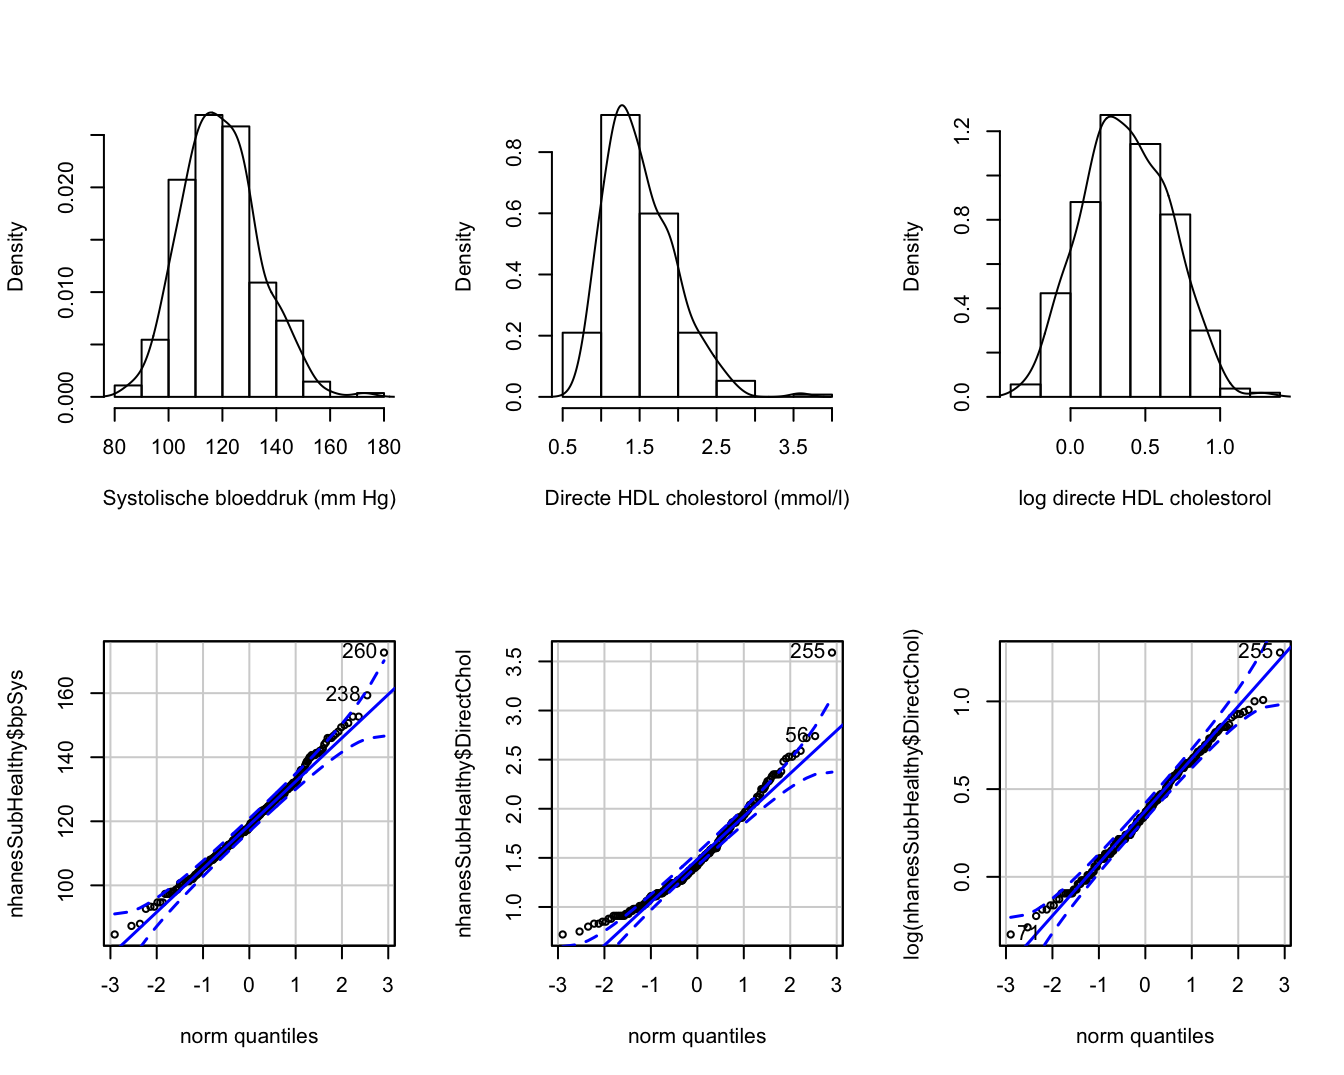
\includegraphics[width=1\linewidth]{Statistiek_2019_2020_files/figure-latex/qqBp-1} 

}

\caption{Kernel density schatters (boven) een QQ-plots (onder) voor de systolische bloeddruk en directe HDL cholestorol bij de subset van gezonde personen tussen de 40 en 65 jaar.}\label{fig:qqBp}
\end{figure}

\begin{verbatim}
## [1] 255  71
\end{verbatim}

De QQ-plot in Figuur \ref{fig:qqBp} (links onder) geeft aan dat de
systolische bloeddruk bij gezonde personen bij benadering Normaal
verdeeld is, hetgeen bevestigd wordt door het histogram met de kernel
density schatter (links boven).\\
Op basis van het gemiddelde van 119.5mmHg en de standaarddeviatie van
14.1 mmHg kunnen we aldus besluiten dat 95\% van de bloeddruk waarden
gelegen zijn tussen de {[}91.9,147{]} mmHg.

De QQ-plot in Figuur \ref{fig:qqBp} (midden en rechts) geeft aan dat de
directe cholestorol bij gezonde personen tussen de 40 en 65 jaar
duidelijk scheef verdeeld is en dat de Normale benadering beter wordt na
log-transformatie. De log-cholestorol is gemiddeld 0.37 en heeft een
standaarddeviatie van 0.29. We kunnen bij benadering stellen dat 95\%
van de log-bloeddrukken liggen tussen {[}-0.19,0.93{]}. Bijgevolg
verwachten we benadering 95\% van de cholestorol metingen tussen
\(\exp(-0.27)=0.76\) en \(\exp(0.85)=2.34\) \(\mu\)mol/l. Deze wijken
ietwat af van de overeenkomstige 2.5\% en 97.5\% percentielen {[}0.87,
2.52{]} \(\mu\)mol/l deels doordat steekproefpercentielen minder precies
(lees: minder stabiel) zijn dan schattingen die men ervoor bekomt op
basis van de Normale verdeling.

\texttt{**Einde\ voorbeeld**}

\section{Samenvattingsmaten voor categorische
variabelen}\label{sec:explCatVar}

De samenvattingsmaten uit de vorige sectie (gemiddelde, mediaan,
standaarddeviatie, \ldots{}) kunnen niet zomaar toegepast worden voor de
beschrijving van categorische variabelen. In deze sectie gaan we hier
dieper op in, daarbij onderscheid makend tussen enerzijds gegevens die
uit prospectieve studies of lukrake steekproeven afkomstig zijn, en
anderzijds gegevens uit retrospectieve studies.

\subsection{Prospectieve studies en lukrake
steekproeven}\label{prospectieve-studies-en-lukrake-steekproeven}

\BeginKnitrBlock{example}[Houtluizen]
\protect\hypertarget{exm:unnamed-chunk-55}{}{\label{exm:unnamed-chunk-55}
\iffalse (Houtluizen) \fi{} }
\EndKnitrBlock{example}

Een bioloog verzamelt `s nachts bladerafval op een lukrake plaats van 1
m\(^2\) in 2 wouden, waarvan 1 met klei- en 1 met kalkgrond. Op elke
plaats telt hij het aantal houtluizen van de species Armadilidium of
Oniscus, met als doel na te gaan of de ene soort vaker voorkomt op
kleigrond dan op kalkgrond\footnote{Merk op dat dit design niet optimaal
  is omdat replicaties op de verkeerde schaal werden bekomen. Idealiter
  moesten meer dan 2 stukken grond in de studie opgenomen worden omdat
  de 2 gekozen stukken grond in veel meer kunnen verschillen dan alleen
  het bodemtype. Verschillen in de verdeling van houtluizen kunnen
  bijgevolg niet zomaar aan het bodemtype kunnen toegeschreven worden.}.
Tabel \ref{tab:cox} toont de bekomen gegevens. Hier stelt \(a\) (\(c\))
het aantal houtluizen van de soort Armadilidium (Oniscus) voor op
kleigrond, en \(b\) (\(d\)) het aantal houtluizen van de soort
Armadilidium (Oniscus) op kalkgrond.

\begin{table}[t]

\caption{\label{tab:cox}Kruistabel van species houtluis versus type grond.}
\centering
\begin{tabular}{llll}
\toprule
  & Armadil. & Oniscus & Totaal\\
\midrule
Klei & 14 (a) & 6 (c) & 20 (a+c)\\
Kalk & 22 (b) & 46 (d) & 68 (b+d)\\
Totaal & 36 (a+b) & 52 (c+d) & 88 (n)\\
\bottomrule
\end{tabular}
\end{table}

\texttt{**Einde\ voorbeeld**}

Er zijn verschillende manieren om de resultaten van deze studie te
beschrijven. De kans dat 1 van beide species houtluizen van de soort
Armadilidium is, is \(p_{kl}=a/(a+c)=0.70\) of 70\% op kleigrond en
\(p_{ka}=b/(b+d)=0.32\) of 32\% op kalkgrond.

\BeginKnitrBlock{definition}[absolute risico verschil]
\protect\hypertarget{def:unnamed-chunk-56}{}{\label{def:unnamed-chunk-56}
\iffalse (absolute risico verschil) \fi{} }Het \textbf{absolute risico
verschil} of absolute kansverschil op een gegeven gebeurtenis (bvb. om
Armadilidium aan te treffen) voor populatie T (Test, bvb. kleigrond)
versus C (Controle, bvb. kalkgrond) wordt met ARV genoteerd en
gedefinieerd als het verschil

\begin{equation*}
ARV=p_T-p_C
\end{equation*}

tussen de kansen dat deze gebeurtenis zich voordoet in populaties T en
C.

\textbf{Einde definitie}
\EndKnitrBlock{definition}

Het ARV op Armadilidium tussen klei- en kalkgrond bedraagt 0.38, hetgeen
suggereert dat de kans dat 1 van beide species houtluizen van de soort
Armadilidium is, 38\% hoger is op kleigrond dan op kalkgrond. Een
absoluut kansverschil van 0 drukt uit dat de overeenkomstige kansen even
groot zijn in beide populaties en dat beide populaties dus vergelijkbaar
zijn in termen van de bestudeerde uitkomst.

Het absolute kansverschil zegt echter niet alles omtrent het bestudeerde
effect. Een kansverschil kan immers een grotere impact hebben
alnaargelang beide proporties \(p_T\) en \(p_C\) dicht bij 0 of 1
liggen, dan wanneer ze in de buurt van 0.5 liggen. Bijvoorbeeld, wanneer
we de proportie vrouwen jonger dan 60 jaar meten die borstkanker
ontwikkelen, is een risicoverschil tussen \(p_A=0.01\) voor vrouwen die
het allel Leu/Leu bezitten op het BRCA1 gen en \(p_B=0.001\) voor de
overige vrouwen, wellicht belangrijker dan een verschil tussen
\(p_C=0.41\) en \(p_D=0.401\) voor beide populaties. Een uitspraak dat
het risico 0.9\% lager is in de ene dan in de andere populatie geeft om
die reden slechts een beperkt beeld van het belang van die reductie. Een
goede vergelijking van risico's, kansen of percentages moet om die reden
ook rekening houden met het basisrisico (d.w.z. de kans op de
bestudeerde uitkomst in een referentiepopulatie). Het ARV doet dit niet,
in tegenstelling tot volgende associatiemaat.

\BeginKnitrBlock{definition}[relatief risico]
\protect\hypertarget{def:unnamed-chunk-57}{}{\label{def:unnamed-chunk-57}
\iffalse (relatief risico) \fi{} }Het \textbf{relatief risico} op een
gegeven gebeurtenis (bvb. om Armadilidium aan te treffen) voor populatie
T (Test, bvb. kleigrond) versus C (Controle, bvb. kalkgrond) wordt met
RR genoteerd en gedefinieerd als het quotiënt

\begin{equation*}
RR=\frac{p_T}{p_C}
\end{equation*}

van de kansen dat deze gebeurtenis zich voordoet in populaties T en C.

\textbf{Einde definitie}
\EndKnitrBlock{definition}

In de studie naar houtluizen bedraagt dit \(RR=0.70/0.32=2.2\). Dit
suggereert dat er 2.2 keer zoveel kans om een houtluis van de soort
Armadilidium (i.p.v. Oniscus) aan te treffen op kleigrond dan op
kalkgrond. Een relatief risico van 1 drukt uit dat beide populaties dus
vergelijkbaar zijn in termen van de bestudeerde uitkomst.

Een nadeel van het relatief risico is dat ze, in tegenstelling tot het
absolute risico verschil, niet goed duidelijk maakt hoeveel meer
individuen de bestudeerde uitkomst ondervinden in de ene dan in de
andere populatie. Bijvoorbeeld, zelfs wetende dat het relatief risico op
Armidilidium in klei-versus kalkgrond 2.2 bedraagt, is het niet mogelijk
om uit te maken hoeveel meer houtluizen van de soort Armidilidium zich
manifesteren op kleigrond. Als de kans om Armidilidium aan te treffen
i.p.v. Oniscus 0.1\% bedraagt op kalkgrond, dan verwacht men dat er per
10000 houtluizen (van de soort Armidilidium of Oniscus) er 10 van de
soort Armidilidium zullen zijn op kalkgrond en 22 op kleigrond, wat
neerkomt op een verwaarloosbaar verschil van 12. Als de kans om
Armidilidium aan te treffen i.p.v. Oniscus 40\% bedraagt op kalkgrond,
dan verwacht men dat er per 10000 houtluizen (van de soort Armidilidium
of Oniscus) er 4000 van de soort Armidilidium zullen zijn op kalkgrond
en 8800 op kleigrond, wat neerkomt op een aanzienlijk verschil van 4800.
Soms rapporteert men in de plaats van het relatief risico, het
\emph{relatieve risico verschil} \(ARV/p_C=RR-1\). Voor de gegeven
studie bedraagt dit 1.2. Het drukt uit dat de toename (van kalk- naar
kleigrond) in kans om Armadilidium aan te treffen succes meer dan 1 keer
zo groot is als het basisrisico in de controlegroep (kalkgrond).

Merk op dat alle bovenstaande associatiematen eveneens gebruikt kunnen
worden wanneer men, in tegenstelling tot wat in een prospectieve studie
gebeurt, een volledig lukrake groep proefpersonen selecteert zonder vast
te leggen hoeveel van hen al dan niet blootgesteld zijn.

\subsection{Retrospectieve studies}\label{subsec:retrospect}

Beschouw de case-controle studie uit Voorbeeld \ref{exm:brcaLeu},
waarvan de gegevens samengevat zijn in Tabel \ref{tab:leu2}. Omdat men
in zo'n design op zoek gaat naar \(a+b+c\) lukraak gekozen controles en
\(d+e+f\) lukraak gekozen cases, liggen de marges \(a+b+c\) en \(d+e+f\)
vast en is het bijgevolg onmogelijk om het risico op case (bvb. risico
op borstkanker) te schatten. Dit is noch mogelijk binnen de totale
groep, noch binnen de groep van blootgestelden (d.i. vrouwen met allel
Leu/Leu), noch binnen de groep niet-blootgestelden. Immers, de kans op
case binnen die geobserveerde groep reflecteert hoofdzakelijk de
verhouding waarin cases en controles in totaal werden gekozen door het
design. Alleen analyses die de kolomtotalen in de tabel vast gegeven
veronderstellen, zijn hier zinvol. Dit heeft tot gevolg dat \emph{het
relatief risico} op de aandoening (d.w.z. op \emph{case}) in de
populatie voor blootgestelden versus niet-blootgestelden niet
rechtstreeks kan geschat worden op basis van gegevens uit een
\emph{case-controle studie}. Analoog kan ook het bijhorende
\emph{absolute risicoverschil niet geschat} worden.

\begin{table}[t]

\caption{\label{tab:leu2}Kruistabel van borstkanker-status versus BRCA1-allel.}
\centering
\begin{tabular}{llll}
\toprule
Genotype & Controles & Cases & Totaal\\
\midrule
Pro/Pro & 266 (a) & 342 (d) & 608 (a+d)\\
Pro/Leu & 250 (b) & 369 (e) & 619 (b+e)\\
Leu/Leu & 56 (c) & 89 (f) & 145 (c+f)\\
Totaal & 572 (a+b+c) & 800 (d+e+f) & 1372 (n)\\
\bottomrule
\end{tabular}
\end{table}

Wel heeft men informatie over de kans om het allel Leu/Leu aan te
treffen bij cases, \(\pi_1=f/(d+e+f)=89/800=11.1\%\), en de kans op het
allel Leu/Leu bij controles, \(\pi_0=c/(a+b+c)=56/572=9.8\%\). Het
relatief risico op blootstelling voor cases versus controles is
bijgevolg \(11.1/9.8=1.14\). Vrouwen met borstkanker hebben dus 14\%
meer kans om de allelcombinatie Leu/Leu te hebben op het BRCA1 gen dan
vrouwen zonder borstkanker. Dit suggereert dat er een
associatie\footnote{Al is het nog de vraag of die associatie toevallig
  is, dan wel systematisch. We komen in het hoofdstuk
  \ref{chap:categorisch}. terug op technieken om dit te onderzoeken.} is
tussen het polymorfisme op het BRCA1 gen en borstkanker, maar drukt
helaas niet uit hoeveel hoger het risico op borstkanker is voor vrouwen
met de allelcombinatie Leu/Leu dan voor andere vrouwen. Om toch een
antwoord te vinden op deze laatste vraag, voeren we een nieuwe
risicomaat in.

\BeginKnitrBlock{definition}[Odds]
\protect\hypertarget{def:unnamed-chunk-58}{}{\label{def:unnamed-chunk-58}
\iffalse (Odds) \fi{} }De \emph{odds} op een gebeurtenis wordt
gedefinieerd als

\begin{equation*}
\frac{p}{1-p}
\end{equation*}

waarbij \(p\) de kans is op die gebeurtenis.

\textbf{Einde definitie}
\EndKnitrBlock{definition}

De odds is dus een transformatie van het risico, met onder andere de
volgende eigenschappen:

\begin{itemize}
\item
  de odds neemt waarden aan tussen nul en oneindig.
\item
  de odds is gelijk aan 1 als en slechts als de kans zelf gelijk is aan
  1/2.
\item
  de odds neemt toe als de kans toeneemt.
\end{itemize}

Het gebruik van odds is populair onder gokkers omdat het uitdrukt
hoeveel waarschijnlijker het is om te winnen dan om te verliezen. Een
odds op winnen gelijk aan 1 drukt bijvoorbeeld uit dat het even
waarschijnlijk is om te winnen dan om te verliezen. Een odds op winnen
gelijk aan 0.9 drukt uit men per 10 verliesbeurten, 9 keer verwacht te
winnen. In de genetische associatiestudie uit Voorbeeld
\ref{exm:brcaLeu} is de odds op allel Leu/Leu bij cases gelijk aan
\(\mbox{odds}_1=f/(d+e)=89/711=0.125\) en bij controles gelijk aan
\(\mbox{odds}_2=c/(a+b)=56/516=0.109\). Vrouwen met borstkanker hebben
bijgevolg ongeveer 8 (\(\approx 1/0.125\)) keer meer kans om de
allelcombinatie Leu/Leu niet te hebben op het BRCA1 gen dan om het wel
te hebben. Om de associatie tussen blootstelling en uitkomst te
beschrijven, kan men nu een verhouding van odds (odds ratio) gebruiken
in plaats van een verhouding van risico's (relatief risico).

\BeginKnitrBlock{definition}[Odds ratio]
\protect\hypertarget{def:unnamed-chunk-59}{}{\label{def:unnamed-chunk-59}
\iffalse (Odds ratio) \fi{} }De \textbf{odds ratio} op een gegeven
gebeurtenis (bvb. borstkanker) voor populatie T (bvb. vrouwen met allel
Leu/Leu) versus C (bvb. vrouwen zonder allel Leu/Leu) wordt met OR
genoteerd en gedefinieerd als het quotiënt

\begin{equation*}
OR=\frac{\mbox{odds}_T}{\mbox{odds}_C}
\end{equation*}

van de odds op deze gebeurtenis in populaties T en C.

\textbf{Einde definitie}
\EndKnitrBlock{definition}

Op basis van de gegevens in Tabel \ref{tab:leu2} kan de odds ratio op
blootstelling voor cases versus controles geschat worden d.m.v. het
kruisproduct

\begin{equation*}
\frac{ \frac{ f/(d+e+f)}{(d+e)/(d+e+f)} }{ \frac{c/(a+b+c)}{(a+b)/(a+b+c)}} = \frac{f(a+b)}{c (d+e)}
\end{equation*}

In het bijzonder vinden we dat de odds op allelcombinatie Leu/Leu voor
vrouwen met versus zonder borstkanker gelijk is aan
\(OR=(89\times 516)/(56\times 711)=1.15\). Helaas drukt dit resultaat
nog steeds niet uit hoeveel meer risico op borstkanker vrouwen met de
allelcombinatie Leu/Leu lopen.

Was de bovenstaande studie echter een volledig lukrake steekproef
geweest (waarbij het aantal cases en controles niet per design werden
vastgelegd), dan konden we daar ook de odds ratio op borstkanker
berekenen voor mensen met versus zonder het allel Leu/leu. We zouden dan
vaststellen dat dit gelijk is aan

\begin{equation*}
\frac{ \frac{ f/(c+f)}{c/(c+f)} }{ \frac{(d+e)/(a+b+d+e)}{(a+b)/(a+b+d+e)}} = \frac{f(a+b)}{c(d+e)},
\end{equation*}

en bijgevolg dezelfde waarde aanneemt. Dat is omdat de odds ratio een
\emph{symmetrische associatiemaat} is zodat de odds ratio op `case' voor
blootgestelden versus niet-blootgestelden steeds gelijk is aan de odds
op blootstelling voor cases versus controles. Hieruit volgt dat voor het
schatten van de odds ratio het er niet toe doet of we prospectief werken
zoals in een typische cohort studie, of retrospectief zoals in een
typische case-controle studie. In het bijzonder kunnen we in de
genetische associatiestudie uit Voorbeeld \ref{exm:brcaLeu} de odds op
borstkanker voor vrouwen met allel Leu/leu versus zonder berekenen als
\(OR=89\times 516/(56\times 711)=1.15\). De odds op borstkanker is
bijgevolg 15\% hoger bij vrouwen met die specifieke allelcombinatie.

Stel nu dat we met \(p_T\) en \(p_C\) respectievelijk de kans op case
noteren voor blootgestelden en niet-blootgestelden. Wanneer beide kansen
klein zijn (namelijk \(p_T<5\%\) en \(p_C<5\%\)), dan is de odds een
goede benadering voor het risico. Dit is omdat in dat geval
\(\mbox{odds}_T=p_T/(1-p_T)\approx p_T\) en
\(\mbox{odds}_C=p_C/(1-p_C)\approx p_C\). Er volgt dan bovendien dat de
odds ratio een goede benadering voor het relatief risico:

\begin{equation*}
OR=\frac{\mbox{ odds}_T}{\mbox{
odds}_C}\approx \frac{p_T}{p_C}=RR
\end{equation*}

Wetende dat het risico op borstkanker laag is, mogen we op basis van de
gevonden OR van 1.15 bijgevolg besluiten dat het risico (i.p.v. de odds)
op borstkanker (bij benadering) 15\% hoger ligt bij vrouwen met het
allel Leu/Leu op het BRCA1 gen. Dit is een bijzonder nuttige eigenschap
omdat (a) het relatief risico, dat niet rechtstreeks geschat kan worden
in case-controle studies, gemakkelijker te interpreteren is dan de odds
ratio; en (b) de odds ratio bepaalde wiskundige eigenschappen heeft die
ze aantrekkelijker maakt dan een relatief risico in statistische
modellen\footnote{Dit is bijvoorbeeld het geval in logistische
  regressiemodellen die gebruikt worden om het risico op een bepaalde
  aandoening te modelleren in functie van prognostische factoren.}.
Algemeen is de odds ratio echter steeds verder van 1 verwijderd dan het
relatief risico. Wetende dat de odds ratio op borstkanker 1.15 bedraagt
voor vrouwen met versus zonder de allelcombinatie Leu/Leu, kunnen we
bijgevolg meer nauwkeurig besluiten dat het overeenkomstige relatief
risico tussen 1 en 1.15 gelegen is (maar niettemin dicht bij 1.15).

Omdat de odds ratio moeilijker te interpreteren is dan een relatief
risico en bijgevolg misleidend kan zijn, valt deze laatste steeds te
verkiezen in situaties (zoals prospectieve studies) waar het mogelijk is
om het relatief risico in de populatie te schatten. In sommige
case-controle studies (nl. matched case-controle studies) wordt voor
elke case een controle gezocht die bepaalde karakteristieken
gemeenschappelijk heeft, teneinde een betere onderlinge
vergelijkbaarheid te garanderen. In dat geval moet de statistische
analyse (inclusief de manier om odds ratio's te schatten) rekening
houden met het feit dat de resultaten van elke case gecorreleerd of
verwant zijn met de resultaten van de bijhorende controle.

\subsection{Rates versus risico's}\label{rates-versus-risicos}

Vaak wordt het begrip \emph{risico} verward met het begrip \emph{rate}.
Een \emph{rate} drukt een aantal gebeurtenissen (bvb. aantal sterfte- of
ziektegevallen) uit per eenheid in de populatie in een bepaalde
tijdspanne. Bijvoorbeeld, een \emph{crude mortality rate (CMR)} voor een
bepaald jaartal is gedefinieerd als 1000 maal het aantal sterftegevallen
dat optreedt in dat jaar gedeeld door de grootte van de beschouwde
populatie halfweg dat jaar. De reden dat met 1000 wordt vermenigvuldigd
is dat het bijvoorbeeld makkelijker na te denken is over een CMR van 12
sterftes per 1000 in Engeland en Wales, dan over 0.012 sterftes per
individu. Indien een specifieke leeftijdsgroep wordt gekozen, verkrijgt
men de \emph{leeftijdsspecifieke mortality rate} als 1000 maal het
aantal sterftegevallen dat optreedt in een bepaald jaar en bepaalde
leeftijdsgroep gedeeld door de grootte van de beschouwde populatie in
die leeftijdsklasse halfweg dat jaar. In tegenstelling tot de
incidentie, is de prevalentie geen rate omdat ze niet een aantal
gebeurtenissen uitdrukt over een zekere tijdspanne.

\section{Associaties tussen twee
variabelen}\label{associaties-tussen-twee-variabelen}

Tot nog toe zijn we hoofdzakelijk ingegaan op zogenaamde univariate
beschrijvingen waarbij slechts 1 variabele onderzocht wordt. In de
meeste wetenschappelijke studies wenst men echter associaties tussen 2
of meerdere variabelen te onderzoeken, bijvoorbeeld tussen een
interventie en de daarop volgende respons. In deze Sectie onderzoeken we
hoe associaties tussen 2 variabelen kunnen beschreven worden. We maken
daarbij onderscheid naargelang het type van de variabelen.

\subsection{Associatie tussen twee kwalitatieve
variabelen}\label{subsec:kruistabel}

Als twee kwalitatieve variabelen niet veel verschillende waarden
aannemen, dan is een \emph{kruistabel} aangewezen om hun associatie voor
te stellen. In deze tabel worden de verschillende waarden die de ene
variabele aanneemt in de kolommen uitgezet en de verschillende waarden
die de andere variabele aanneemt in de rijen. In elke cel van de tabel
(die overeenkomt met 1 specifieke combinatie van waarden voor beide
variabelen) wordt de frequentie neergeschreven.

\begin{table}[t]

\caption{\label{tab:genderBMI}Kruistabel van Gender vs BMI klasse.}
\centering
\begin{tabular}{lrrrr}
\toprule
  & 12.0\_18.5 & 18.5\_to\_24.9 & 25.0\_to\_29.9 & 30.0\_plus\\
\midrule
female & 629 & 1616 & 1179 & 1402\\
male & 648 & 1295 & 1485 & 1349\\
\bottomrule
\end{tabular}
\end{table}

Tabel \ref{tab:genderBMI} toont zo'n kruistabel voor het aantal mannen
en vrouwen per BMI klasse. Dergelijke eenvoudige kruistabel met slechts
2 rijen en 4 kolommen, noemt men ook een \(2\times 4\) tabel.

\subsection{Associatie tussen één kwalitatieve en één continue
variabele}\label{subsec:asskwalcont}

De eenvoudigste grafische weergave met het maximum aan informatie om de
associatie tussen een kwalitatieve en een continue variabele te
beschrijven is een \emph{dot-plot}.

\begin{Shaded}
\begin{Highlighting}[]
\KeywordTok{ggplot}\NormalTok{(NHANES[}\DecValTok{1}\OperatorTok{:}\DecValTok{100}\NormalTok{, ], }\KeywordTok{aes}\NormalTok{(}\DataTypeTok{x =}\NormalTok{ Gender, }\DataTypeTok{y =} \KeywordTok{log}\NormalTok{(DirectChol))) }\OperatorTok{+}\StringTok{ }
\StringTok{    }\KeywordTok{geom_dotplot}\NormalTok{(}\DataTypeTok{binaxis =} \StringTok{"y"}\NormalTok{, }\DataTypeTok{stackdir =} \StringTok{"center"}\NormalTok{)}
\end{Highlighting}
\end{Shaded}

\begin{figure}

{\centering 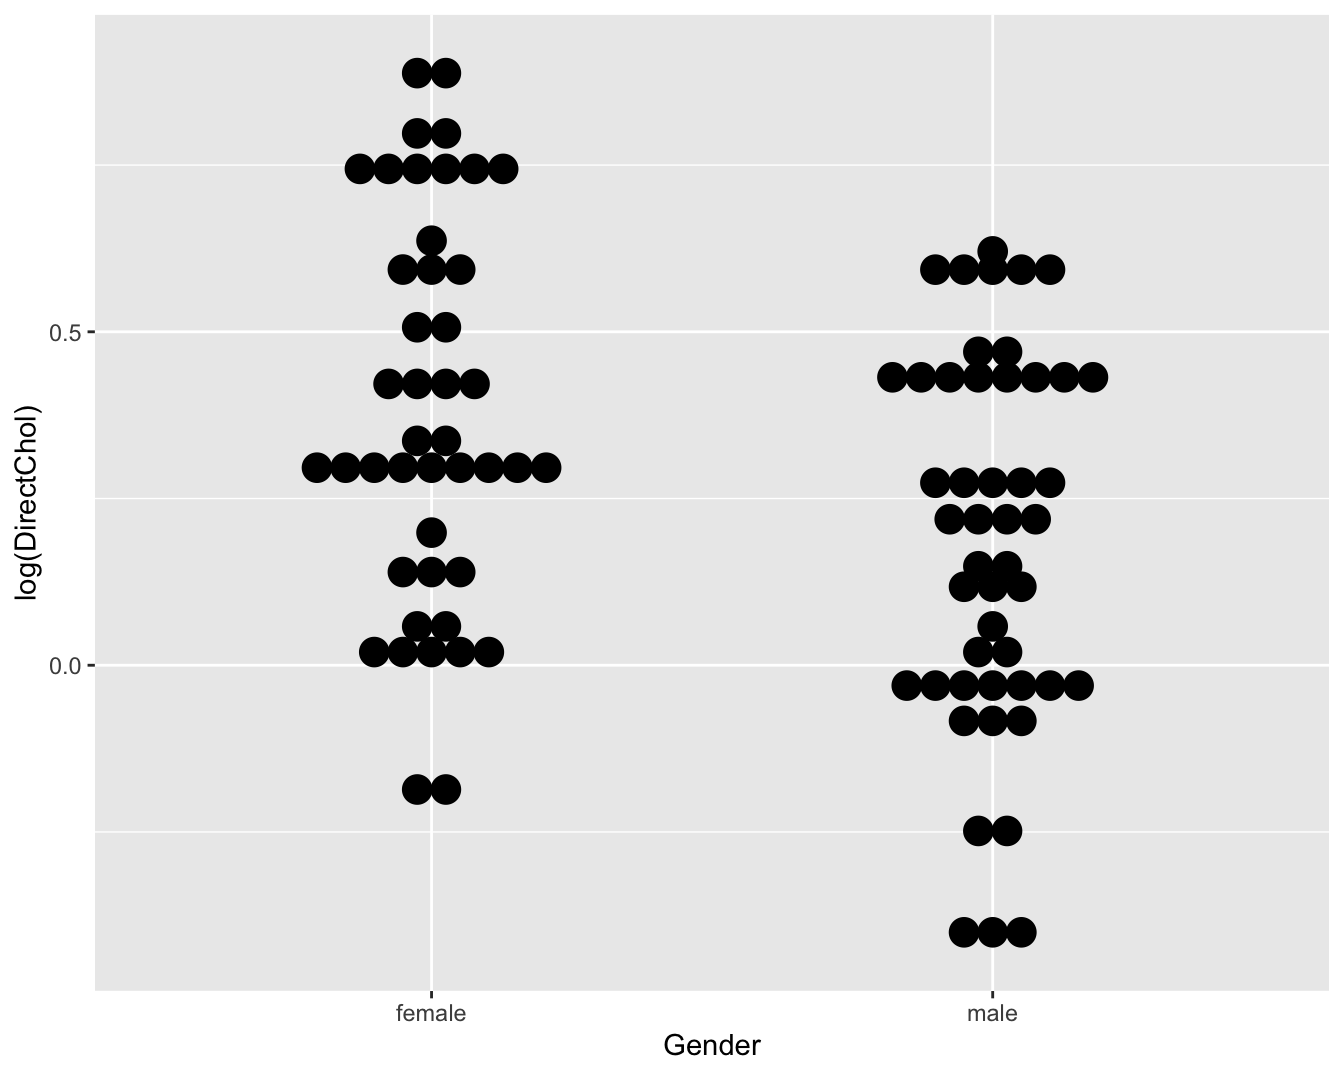
\includegraphics[width=1\linewidth]{Statistiek_2019_2020_files/figure-latex/dotCholGender-1} 

}

\caption{Dotplot van log-getransformeerde directe HDL cholestorol concentratie in functie van Gender voor de eerste 100 subjecten van de NHANES studie.}\label{fig:dotCholGender}
\end{figure}

Dit wordt geïllustreerd in Figuur \ref{fig:dotCholGender} waarbij de log
directe cholestorol concentratie is geplot in functie van het geslacht
voor de eerste 100 personen in de studie. Deze voorstellingsmethode
behoudt de individuele waarden van de observaties en laat gemakkelijke
vergelijkingen toe tussen de verschillende groepen. Een bijkomend
voordeel is dat outliers meteen zichtbaar zijn in een dot-plot. Een
nadeel ontstaat wanneer de steekproef groot is en bijgevolg vele
observaties samenvallen op de figuur. Vandaar dat we de plot hebben
gemaakt voor een subset van de data.

Als het aantal observaties groot is, kan een dot-plot vervangen worden
door \emph{boxplots}. Deze is meer compact dan een histogram en laat om
die reden gemakkelijker vergelijkingen tussen verschillende groepen toe.
Twee dergelijke boxplots worden getoond in Figuur
\ref{fig:boxplotCholGender}.

\begin{Shaded}
\begin{Highlighting}[]
\KeywordTok{boxplot}\NormalTok{(}\KeywordTok{log}\NormalTok{(DirectChol) }\OperatorTok{~}\StringTok{ }\NormalTok{Gender, }\DataTypeTok{data =}\NormalTok{ NHANES, }\DataTypeTok{ylab =} \StringTok{"log(Direct Cholestorol)"}\NormalTok{)}
\end{Highlighting}
\end{Shaded}

\begin{figure}

{\centering 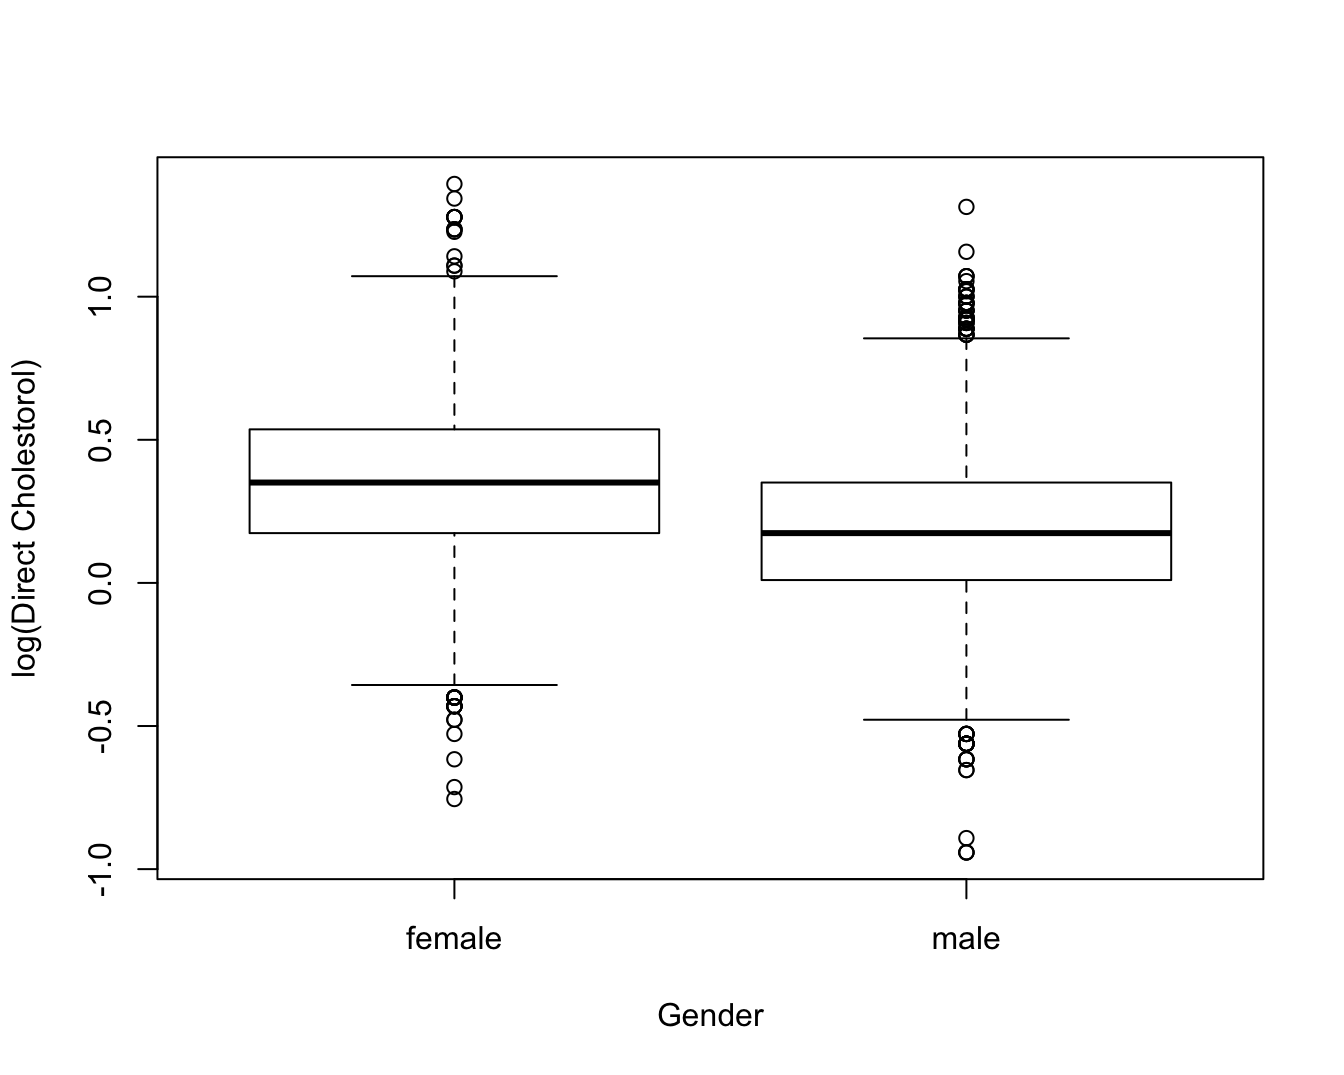
\includegraphics[width=1\linewidth]{Statistiek_2019_2020_files/figure-latex/boxplotCholGender-1} 

}

\caption{Dotplot van log-getransformeerde directe HDL cholestorol concentratie in functie van Gender voor alle subjecten van de NHANES studie.}\label{fig:boxplotCholGender}
\end{figure}

Op basis van deze figuur stellen we vast dat hogere log-cholestorol
concentraties geobserveerd worden bij vrouwen dan bij mannen, maar dat
de variabiliteit van de log-concentraties vergelijkbaar is tussen de 2
groepen. De vraag blijft of we hier kunnen spreken van een systematisch
hogere log-cholestorol concentratie tussen vrouwen en mannen. We zullen
in Hoofdstuk \ref{chap:besluit} dieper op deze vraag ingaan.

Figuur \ref{fig:boxplotCholGender} kan men samenvatten door gemiddelde
verschillen tussen beide groepen te rapporteren. Hier stellen we een
gemiddeld verschil van 0.17 in directe HDL cholestorol concentratie vast
op de log schaal tussen vrouwen en mannen. Gezien we weten dat
\(\log(C_2)-\log(C_1)=\log(C_2/C_1)\) besluiten we dat de HDL
cholestorol concentratie in de NHANES studie gemiddeld 1.19 keer hoger
ligt voor vrouwen dan voor mannen.

Dot-plots zijn bijzonder interessant in pre-test post-test designs waar
dezelfde subjecten op verschillende tijdstippen worden geobserveerd. In
dat geval kunnen de uitkomsten uitgezet worden op de Y-as en de
tijdstippen op de X-as, en kunnen de metingen voor eenzelfde subject
worden verbonden met een lijn.

Een voorbeeld hiervan is weergegeven in Figuur \ref{fig:captoDot}. De
figuur vat de gegevens samen van de captopril studie die de centrale
dataset vormt van Hoofdstuk \ref{chap:besluit}. In de studie wenst men
het effect van een bloeddrukverlagend geneesmiddel captopril evalueren.
Voor elke patiënt in de studie werd de systolische bloeddruk twee keer
gemeten: één keer voor en één keer na de behandeling met het bloeddruk
verlagende medicijn captopril. In Figuur \ref{fig:captoDot} worden de
metingen van dezelfde patiënt met een lijntje verbonden. Hierdoor
krijgen we een heel duidelijk beeld van de gegevens. Namelijk, we
krijgen een sterke indruk dat de bloeddruk daalt na het toedienen van
captopril gezien we bijna voor alle patiënten een daling observeren.

\begin{verbatim}
##   id SBPb DBPb SBPa DBPa
## 1  1  210  130  201  125
## 2  2  169  122  165  121
## 3  3  187  124  166  121
## 4  4  160  104  157  106
## 5  5  167  112  147  101
## 6  6  176  101  145   85
\end{verbatim}

\begin{figure}

{\centering 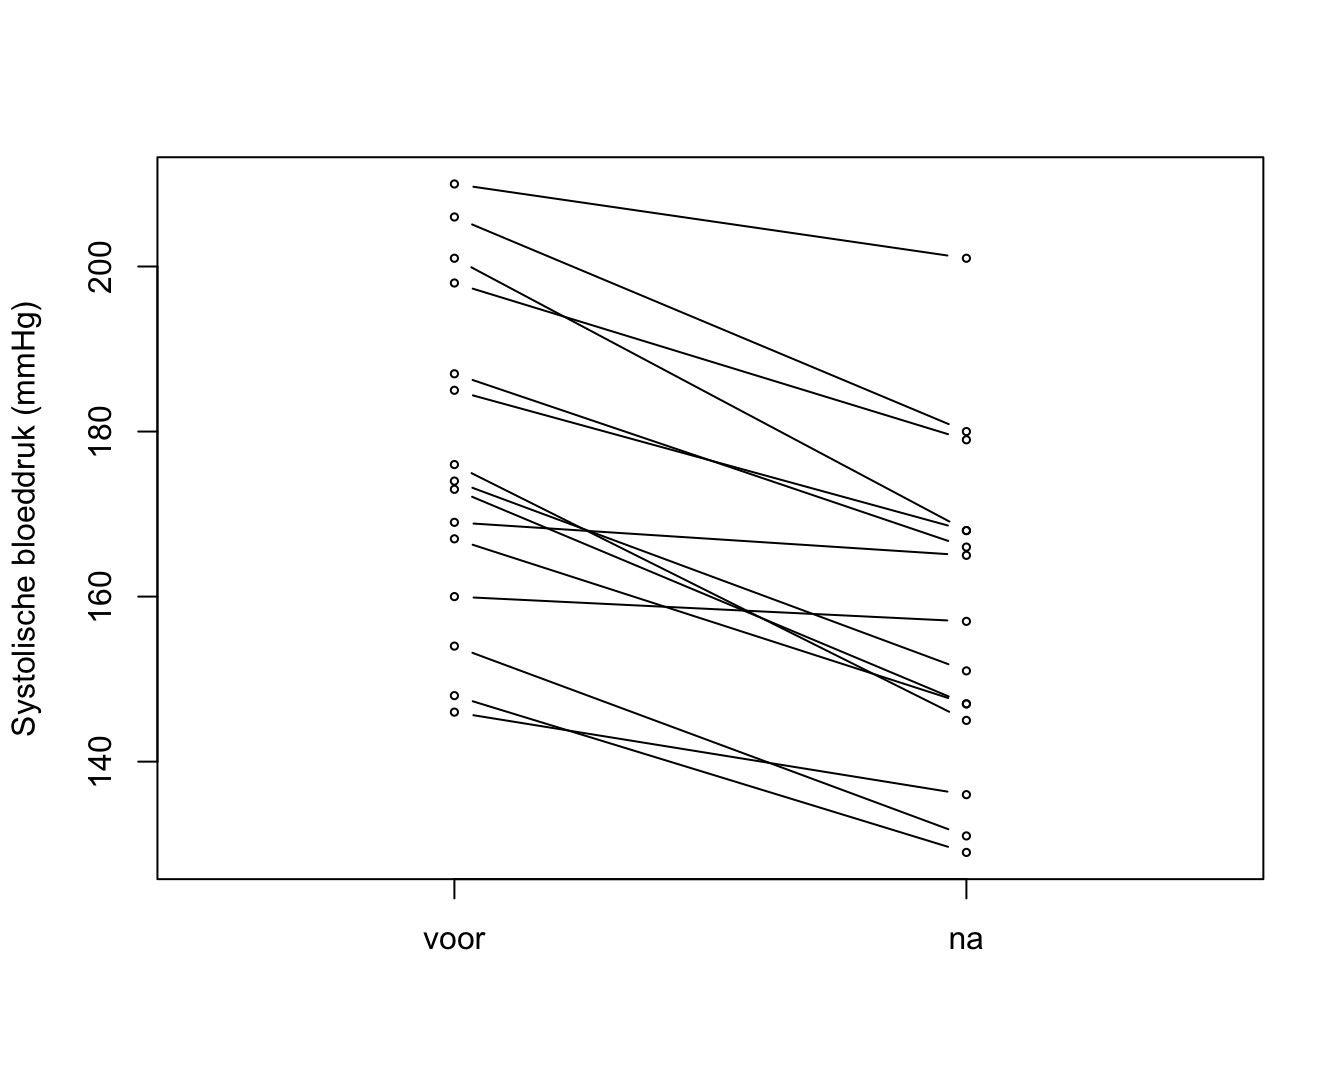
\includegraphics[width=1\linewidth]{Statistiek_2019_2020_files/figure-latex/captoDot-1} 

}

\caption{Dotplot van de systolische bloeddruk in de captopril studie voor en na het toedienen van het bloeddruk verlagend middel captopril.}\label{fig:captoDot}
\end{figure}

\subsection{Associatie tussen twee continue
variabelen}\label{sec:correlatie}

De associatie tussen 2 kwantitatieve variabelen kan worden onderzocht
aan de hand van een \emph{puntenwolk} of \emph{spreidingsdiagram} (in
het Engels: \emph{scatterplot}). Hier worden de geobserveerde waarden
van de ene variabele uitgezet tegen de andere. In Hoofdstuk
\ref{chap:linReg} wordt gewerkt rond een centrale dataset m.b.t.
borstkanker. Voor 32 borstkanker patiënten werd gen-expressie gemeten
van de tumor a.d.h.v. microarray technologie. Figuur
\ref{fig:brcaLogFit} zet de log-expressie uit van het S100A8 gen ten
opzichte van estrogen recepter gen (ESR1). Beide genen spelen een
belangrijke rol in kanker. Expressie van het ESR1 gen is een indicator
dat de tumor vatbaar is voor hormoontherapie wat gunstig is voor de
prognose. Het S100A8-gen daarentegen is betrokken bij de onderdrukking
van het immuunsysteem en het gen speelt een rol in het creëren van een
inflamatoir milieu in de tumor.

\begin{Shaded}
\begin{Highlighting}[]
\NormalTok{borstkanker =}\StringTok{ }\KeywordTok{read.table}\NormalTok{(}\StringTok{"dataset/borstkanker.txt"}\NormalTok{, }
    \DataTypeTok{header =} \OtherTok{TRUE}\NormalTok{)}
\KeywordTok{with}\NormalTok{(borstkanker, }\KeywordTok{scatter.smooth}\NormalTok{(}\KeywordTok{log2}\NormalTok{(ESR1), }\KeywordTok{log2}\NormalTok{(S100A8), }
    \DataTypeTok{lpars =} \KeywordTok{list}\NormalTok{(}\DataTypeTok{lty =} \DecValTok{2}\NormalTok{)))}
\end{Highlighting}
\end{Shaded}

\begin{figure}

{\centering 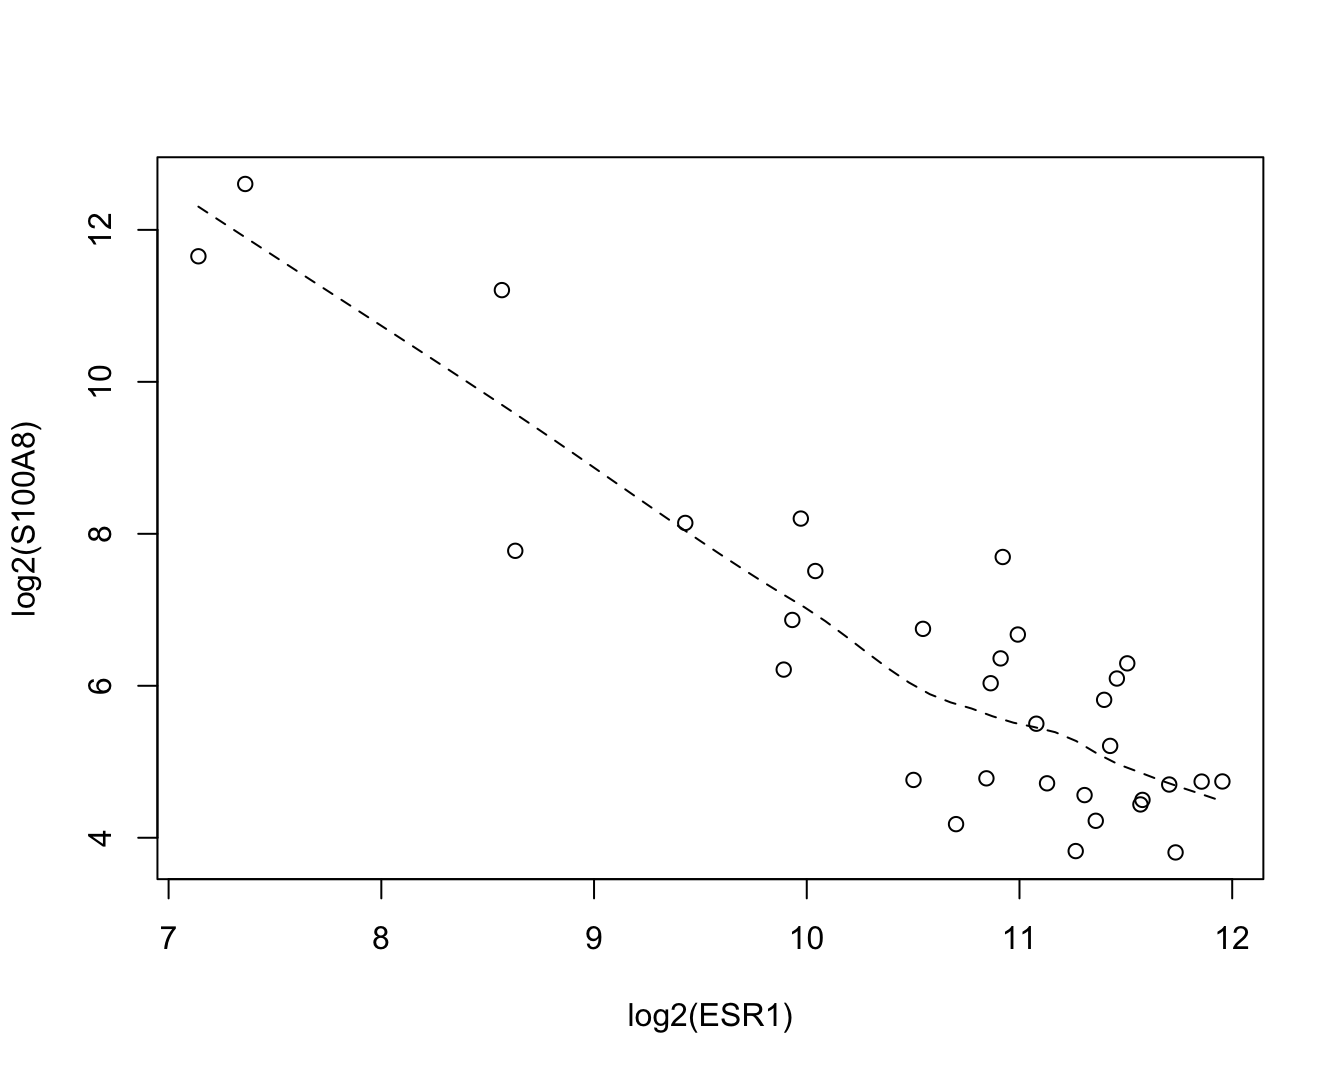
\includegraphics[width=1\linewidth]{Statistiek_2019_2020_files/figure-latex/brcaLogFit-1} 

}

\caption{Expressie van het S100A8 gen in functie van de ESR1 gen-expressie.}\label{fig:brcaLogFit}
\end{figure}

De lijn op de figuur is een \emph{(niet-parametrische) regressielijn}.
Deze vat de associatie tussen beide variabelen samen door de gemiddelde
log2-expressie voor S100A8 weer te geven in functie van de
log2-expressie van het ESR1 gen.

We observeren in Figuur \ref{fig:brcaLogFit} een negatieve associatie
tussen de S100A8 en ESR1 expressie. De expressie van S100A8 neemt
gemiddeld gezien af bij patiënten waar het ESR1 gen hoger geëxpresseerd
is.

In de praktijk wenst men de sterkte van de samenhang tussen 2 continue
variabelen graag ook beknopt uit te kunnen drukken d.m.v. een
samenvattingsmaat. Zo'n veelgebruikte maat om de \emph{lineaire}
samenhang tussen 2 continue metingen uit te drukken, is de
\emph{(Pearson) correlatiecoëfficiënt} of kortweg \emph{correlatie}.

\BeginKnitrBlock{definition}[Correlatie]
\protect\hypertarget{def:unnamed-chunk-60}{}{\label{def:unnamed-chunk-60}
\iffalse (Correlatie) \fi{} }Stel dat \(x_{i}\) (bvb. lengte) en
\(y_{i}\) (bvb. gewicht) 2 metingen zijn die opgemeten werden bij
eenzelfde individu \(i=1,...,n\). Dan wordt de \textbf{Pearson
correlatie} tussen de rij getallen \(x\) en \(y\) gedefinieerd als:

\begin{equation*}
\mbox{Cor}(x,y)=\frac{\sum_{i=1}^{n}(x_{i}-\bar{x})(y_{i}-\bar{y})}{
(n-1)s_{x}s_{y}},
\end{equation*}

met \(s_{x}\) en \(s_{y}\) de standaarddeviatie van respectievelijk de
rij getallen \(x\) en \(y\). De Pearson correlatie wordt typisch met
\(r\) genoteerd.

\textbf{Einde definitie}
\EndKnitrBlock{definition}

De teller in bovenstaande uitdrukking gaat na in welke mate positieve
(negatieve) afwijkingen tussen \(x\) en zijn gemiddelde samengaan met
positieve of negatieve afwijkingen tussen \(y\) en zijn gemiddelde. Het
teken van de correlatie geeft bijgevolg de richting van de lineaire
trend aan: het teken is positief (negatief) wanneer hogere waarden voor
de ene variabele samengaan met hogere (lagere) waarden voor de andere.
Men zegt in dat geval dat er een \emph{positieve (negatieve) associatie}
is. De noemer in de uitdrukking standaardiseert het geheel waardoor,
zoals men wiskundig kan aantonen, de correlatie(coëfficiënt) een getal
is gelegen tussen -1 en 1. Uitkomsten die perfect lineair afhankelijk
zijn van elkaar (d.w.z. dat ze in een scatterplot gelegen zijn op een
rechte lijn) hebben een correlatie van 1 of -1. \emph{Onafhankelijke
variabelen} (d.w.z. variabelen waarvoor kennis van de waarde voor de ene
variabele geen informatie levert over de waarde voor de andere
variabele) hebben een correlatie gelijk aan 0.

De correlatie tussen de log2-S100A8 en log2-ESR1 expressie bedraagt
-0.89. Wat opnieuw op een sterke negatieve correlatie wijst tussen de
log-expressie van beide genen.

\begin{Shaded}
\begin{Highlighting}[]
\KeywordTok{par}\NormalTok{(}\DataTypeTok{mfrow =} \KeywordTok{c}\NormalTok{(}\DecValTok{2}\NormalTok{, }\DecValTok{3}\NormalTok{))}
\ControlFlowTok{for}\NormalTok{ (i }\ControlFlowTok{in} \KeywordTok{c}\NormalTok{(}\FloatTok{0.3}\NormalTok{, }\FloatTok{0.7}\NormalTok{, }\FloatTok{0.99}\NormalTok{, }\OperatorTok{-}\FloatTok{0.3}\NormalTok{, }\OperatorTok{-}\FloatTok{0.5}\NormalTok{, }\OperatorTok{-}\FloatTok{0.9}\NormalTok{)) }\KeywordTok{plot}\NormalTok{(}\KeywordTok{rmvnorm}\NormalTok{(}\DecValTok{100}\NormalTok{, }
    \DataTypeTok{sigma =} \KeywordTok{matrix}\NormalTok{(}\KeywordTok{c}\NormalTok{(}\DecValTok{1}\NormalTok{, i, i, }\DecValTok{1}\NormalTok{), }\DataTypeTok{ncol =} \DecValTok{2}\NormalTok{)), }\DataTypeTok{xlab =} \StringTok{"x"}\NormalTok{, }
    \DataTypeTok{ylab =} \StringTok{"y"}\NormalTok{, }\DataTypeTok{main =} \KeywordTok{paste}\NormalTok{(}\StringTok{"correlatie"}\NormalTok{, i))}
\end{Highlighting}
\end{Shaded}

\begin{figure}

{\centering 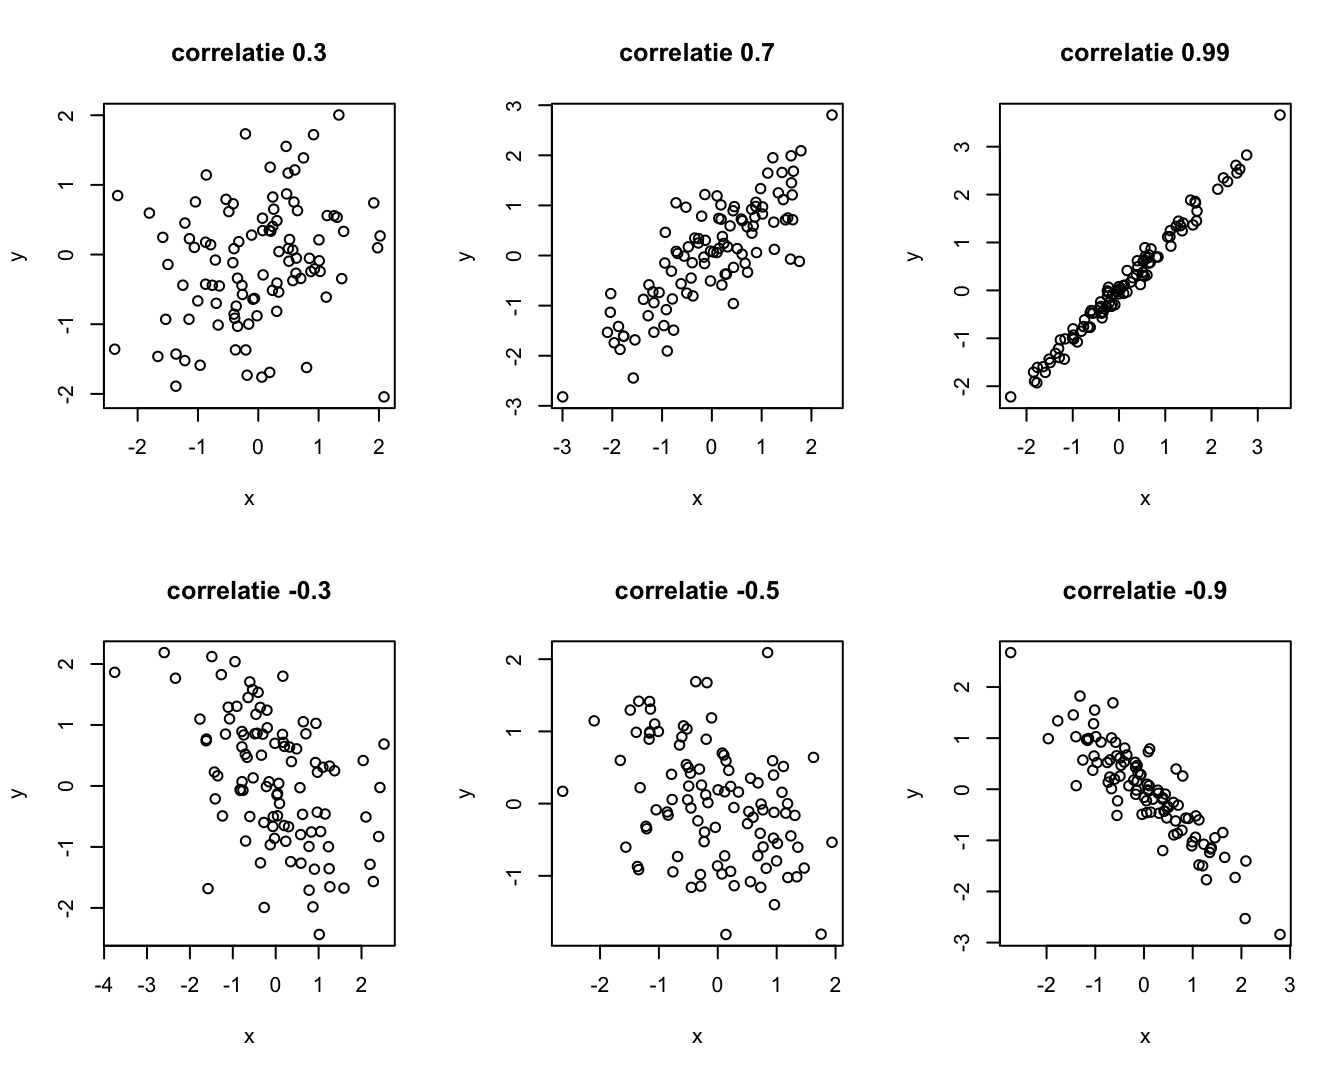
\includegraphics[width=1\linewidth]{Statistiek_2019_2020_files/figure-latex/regr1-1} 

}

\caption{Gesimuleerde gegevens met verschillende correlatie.}\label{fig:regr1}
\end{figure}

Figuur \ref{fig:regr1} toont ter illustratie verschillende scatterplots
waar fictieve gegevens met verschillende correlaties werden gesimuleerd.
Merk op dat het lineaire patroon tussen de twee reeksen gegevens sterker
wordt met toenemende correlatie en van richting wijzigt naarmate de
correlatie negatief wordt.

\textbf{Eigenschap}

De correlatie tussen 2 reeksen metingen \((x_i)\) en \((y_i)\) blijft
ongewijzigd

\begin{itemize}
\item
  wanneer bij alle uitkomsten \(x_i\) een willekeurige constante \(a\)
  wordt opgeteld;
\item
  wanneer alle uitkomsten \(x_i\) met een willekeurige constante \(a\)
  worden vermenigvuldigd;
\item
  wanneer \((x_i,\bar x)\) en \((y_i,\bar y)\) van plaats worden
  verwisseld in de uitdrukking voor de correlatie.
\end{itemize}

\textbf{Einde eigenschap}

Op basis van deze eigenschap kunnen we bijvoorbeeld besluiten dat de
correlatie tussen de expressie van het S100A8 en ESR1 gen niet gewijzigd
wordt wanneer we een log10 transformatie hadden gebruikt ipv een log2
tranformatie. Door de eigenschappen van logaritmes weten we immers dat
\(\log_{2}(x)=\log_{10}(x)/\log_{10}(2)\)

\begin{Shaded}
\begin{Highlighting}[]
\KeywordTok{set.seed}\NormalTok{(}\DecValTok{100}\NormalTok{)}
\CommentTok{# Een seed wordt gebruikt om ervoor te zorgen dat}
\CommentTok{# dezelfde resultaten opnieuw kunnen worden bekomen}
\CommentTok{# wanneer men at random data genereerd}
\KeywordTok{par}\NormalTok{(}\DataTypeTok{mfrow =} \KeywordTok{c}\NormalTok{(}\DecValTok{1}\NormalTok{, }\DecValTok{2}\NormalTok{))  }\CommentTok{#twee plots naast elkaar}
\CommentTok{# simuleer}
\NormalTok{scheef =}\StringTok{ }\KeywordTok{exp}\NormalTok{(}\KeywordTok{rmvnorm}\NormalTok{(}\DecValTok{100}\NormalTok{, }\DataTypeTok{mean =} \KeywordTok{rep}\NormalTok{(}\FloatTok{1.5}\NormalTok{, }\DecValTok{2}\NormalTok{), }\DataTypeTok{sigma =} \KeywordTok{matrix}\NormalTok{(}\KeywordTok{c}\NormalTok{(}\FloatTok{1.5}\NormalTok{, }
    \FloatTok{0.75} \OperatorTok{*}\StringTok{ }\FloatTok{1.5}\NormalTok{, }\FloatTok{0.75} \OperatorTok{*}\StringTok{ }\FloatTok{1.5}\NormalTok{, }\FloatTok{1.5}\NormalTok{), }\DataTypeTok{ncol =} \DecValTok{2}\NormalTok{)))}
\CommentTok{# plot}
\KeywordTok{plot}\NormalTok{(scheef, }\DataTypeTok{main =} \KeywordTok{paste}\NormalTok{(}\StringTok{"Correlatie"}\NormalTok{, }\KeywordTok{round}\NormalTok{(}\KeywordTok{cor}\NormalTok{(scheef)[}\DecValTok{1}\NormalTok{, }
    \DecValTok{2}\NormalTok{], }\DecValTok{2}\NormalTok{)), }\DataTypeTok{xlab =} \StringTok{"x"}\NormalTok{, }\DataTypeTok{ylab =} \StringTok{"y"}\NormalTok{)}
\CommentTok{# simuleer}
\NormalTok{normal <-}\StringTok{ }\KeywordTok{rmvnorm}\NormalTok{(}\DecValTok{100}\NormalTok{, }\DataTypeTok{mean =} \KeywordTok{rep}\NormalTok{(}\FloatTok{1.5}\NormalTok{, }\DecValTok{2}\NormalTok{), }\DataTypeTok{sigma =} \KeywordTok{matrix}\NormalTok{(}\KeywordTok{c}\NormalTok{(}\FloatTok{1.5}\NormalTok{, }
    \FloatTok{0.71} \OperatorTok{*}\StringTok{ }\FloatTok{1.5}\NormalTok{, }\FloatTok{0.71} \OperatorTok{*}\StringTok{ }\FloatTok{1.5}\NormalTok{, }\FloatTok{1.5}\NormalTok{), }\DataTypeTok{ncol =} \DecValTok{2}\NormalTok{))}
\CommentTok{# plot}
\KeywordTok{plot}\NormalTok{(normal, }\DataTypeTok{main =} \KeywordTok{paste}\NormalTok{(}\StringTok{"Correlatie"}\NormalTok{, }\KeywordTok{round}\NormalTok{(}\KeywordTok{cor}\NormalTok{(normal)[}\DecValTok{1}\NormalTok{, }
    \DecValTok{2}\NormalTok{], }\DecValTok{2}\NormalTok{)), }\DataTypeTok{xlab =} \StringTok{"x"}\NormalTok{, }\DataTypeTok{ylab =} \StringTok{"y"}\NormalTok{)}
\end{Highlighting}
\end{Shaded}

\begin{figure}

{\centering 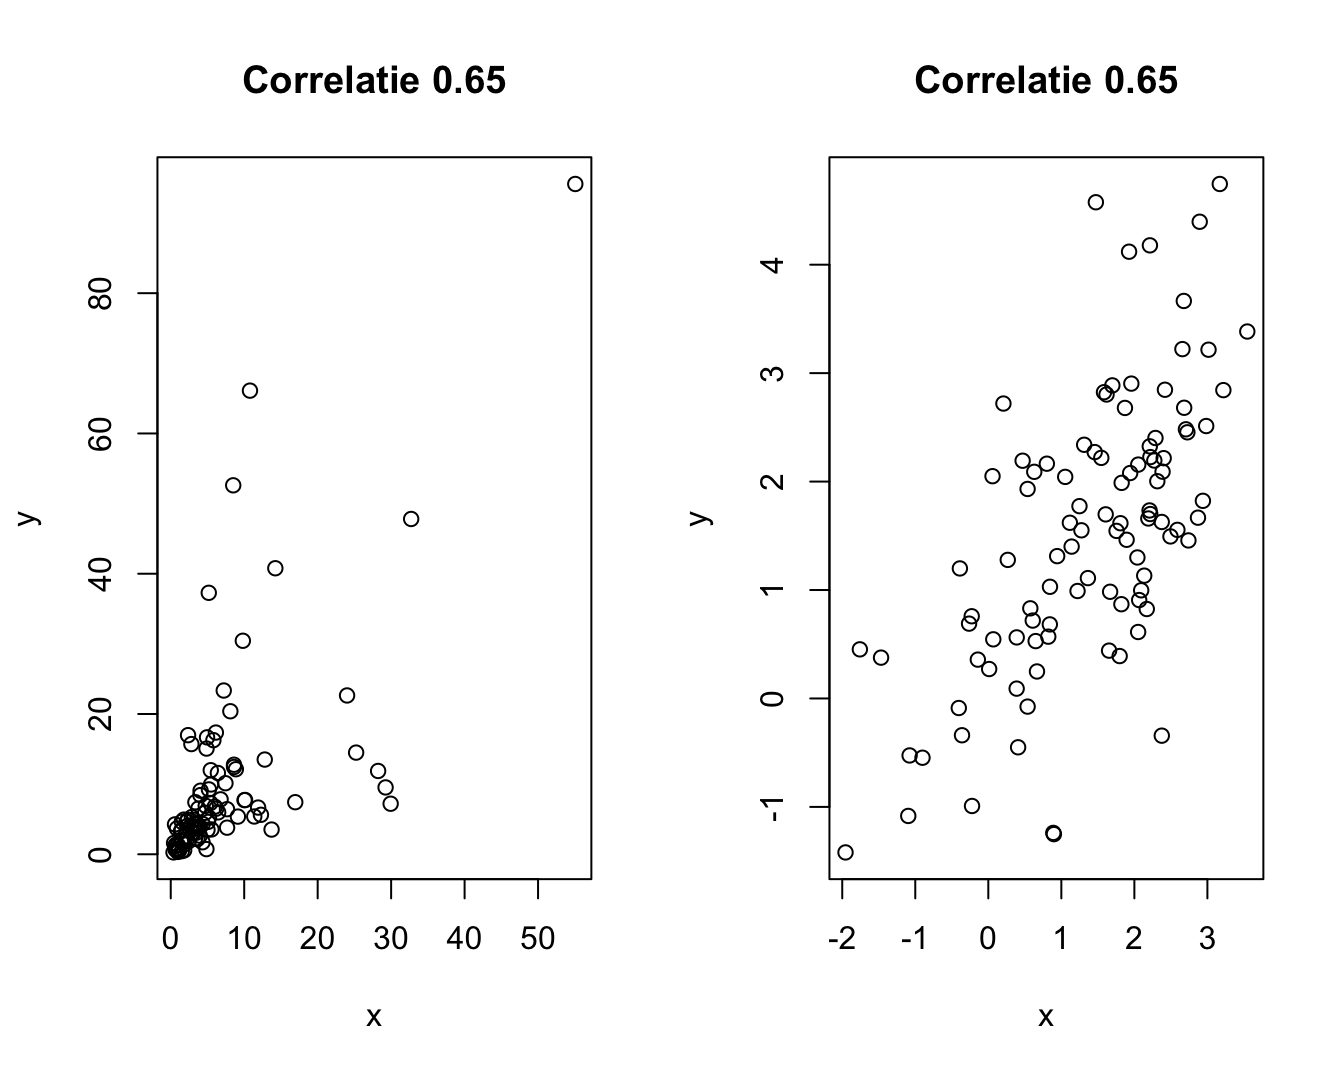
\includegraphics[width=1\linewidth]{Statistiek_2019_2020_files/figure-latex/regr3-1} 

}

\caption{Links: scheef verdeelde observaties; Rechts: Normaal verdeelde observaties.}\label{fig:regr3}
\end{figure}

Bij het interpreteren van correlaties, alsook bij het uitvoeren van
regressie-analyses in de volgende secties, zijn de volgende
waarschuwingen van zeer groot belang:

\begin{enumerate}
\def\labelenumi{\arabic{enumi}.}
\tightlist
\item
  Correlaties zijn het makkelijkst te interpreteren tussen 2 groepen
  Normaal verdeelde observaties. Een kleine training laat immers toe om
  snel inzicht te krijgen in de grootte van de correlatiecoëfficiënt
  zonder zich verder over de specifieke verdeling te hoeven bekommeren.
  In het bijzonder kan men voor Normaal verdeelde observaties visueel
  inzicht krijgen in de sterkte van de correlatie door een ellips rond
  de puntenwolk te tekenen die (nagenoeg) alle punten bevat. Als de
  ellips op een cirkel lijkt, dan is er geen correlatie. Hoe dunner de
  ellips, hoe sterker de correlatie. De oriëntatie van de ellips geeft
  hierbij het teken van de correlatie weer.
\end{enumerate}

Voor niet-Normale gegevens hangt de betekenis van een
correlatiecoëfficiënt van zekere grootte, nauw samen met de specifieke
vorm van de verdeling. Figuur \ref{fig:regr3} toont ter illustratie 1
paar scheef verdeelde (links) en 1 paar Normaal verdeelde (rechts)
observaties. Hoewel de correlatie in beide figuren 0.65 bedraagt, tonen
beide figuren een verschillende associatie. Merk ook op in Figuur
\ref{fig:regr2} (rechts) dat de grootte van de correlatie sterk
beïnvloed kan worden door een paar outliers. De correlatie tussen deze
variabelen bedraagt slechts 0.44, maar 0.93 na verwijdering van de 2
outliers.

Wanneer de 2 variabelen die we onderzoeken niet Normaal verdeeld zijn,
dan zijn er 2 mogelijkheden om een zinvolle correlatiecoëfficiënt weer
te geven. Variabelen die scheef verdeeld zijn, kan men transformeren
(bvb. een log-transformatie) in de hoop dat de getransformeerde gegevens
bij benadering Normaal verdeeld zijn en lineair samenhangen. Bemerk dat
we de genexpressie van S100A8 en ESR1 daarom log-getransformeerd hebben
in Figuur \ref{fig:brcaLogFit}, concentraties en intensiteitsmetingen
zijn immers vaak log-normaal verdeeld.

Indien transformatie niet helpt of wanneer er outliers zijn, kan men een
meer \emph{robuuste} maat voor de samenhang tussen 2 variabelen
rapporteren, zoals de \emph{Spearman's rank correlatie}. Dit is per
definitie de Pearson correlatiecoëfficiënt van de \emph{rangen} van de 2
beschouwde variabelen. Dergelijke rangen worden bekomen door voor elke
variabele afzonderlijk de metingen te vervangen door de rangorde waarin
ze voorkomen. In het bijzonder krijgt de kleinste meting rangorde 1
toegekend, de tweede kleinste rangorde 2, etc. Door aldus rangordes voor
de 2 variabelen afzonderlijk te nemen, blijft de samenhang ruwweg
behouden, maar wordt de invloed van outliers gevoelig afgezwakt (omdat
rangordes relatief gezien nooit extreem worden).

\begin{Shaded}
\begin{Highlighting}[]
\KeywordTok{par}\NormalTok{(}\DataTypeTok{mfrow =} \KeywordTok{c}\NormalTok{(}\DecValTok{1}\NormalTok{, }\DecValTok{2}\NormalTok{))}
\KeywordTok{set.seed}\NormalTok{(}\DecValTok{34}\NormalTok{)}
\NormalTok{x =}\StringTok{ }\KeywordTok{c}\NormalTok{(}\KeywordTok{rnorm}\NormalTok{(}\DecValTok{100}\NormalTok{))}
\NormalTok{y =}\StringTok{ }\DecValTok{3} \OperatorTok{*}\StringTok{ }\NormalTok{x}\OperatorTok{^}\DecValTok{2} \OperatorTok{+}\StringTok{ }\KeywordTok{rnorm}\NormalTok{(}\DecValTok{100}\NormalTok{, }\DataTypeTok{sd =} \DecValTok{2}\NormalTok{)}
\KeywordTok{plot}\NormalTok{(x, y, }\DataTypeTok{main =} \KeywordTok{paste}\NormalTok{(}\StringTok{"Correlation"}\NormalTok{, }\KeywordTok{round}\NormalTok{(}\KeywordTok{cor}\NormalTok{(x, }
\NormalTok{    y), }\DecValTok{2}\NormalTok{)))}
\NormalTok{simHlp =}\StringTok{ }\KeywordTok{matrix}\NormalTok{(}\DecValTok{0}\NormalTok{, }\DataTypeTok{ncol =} \DecValTok{2}\NormalTok{, }\DataTypeTok{nrow =} \DecValTok{20}\NormalTok{)}
\NormalTok{simHlp[}\DecValTok{1}\OperatorTok{:}\DecValTok{18}\NormalTok{, ] =}\StringTok{ }\KeywordTok{rmvnorm}\NormalTok{(}\DecValTok{18}\NormalTok{, }\DataTypeTok{sigma =} \KeywordTok{matrix}\NormalTok{(}\KeywordTok{c}\NormalTok{(}\DecValTok{1}\NormalTok{, }\FloatTok{0.9}\NormalTok{, }
    \FloatTok{0.9}\NormalTok{, }\DecValTok{1}\NormalTok{), }\DataTypeTok{ncol =} \DecValTok{2}\NormalTok{))}
\NormalTok{simHlp[}\DecValTok{19}\OperatorTok{:}\DecValTok{20}\NormalTok{, ] =}\StringTok{ }\KeywordTok{cbind}\NormalTok{(}\KeywordTok{max}\NormalTok{(simHlp[, }\DecValTok{1}\NormalTok{]) }\OperatorTok{*}\StringTok{ }\KeywordTok{c}\NormalTok{(}\FloatTok{1.1}\NormalTok{, }\FloatTok{1.3}\NormalTok{), }
    \KeywordTok{c}\NormalTok{(}\OperatorTok{-}\DecValTok{2}\NormalTok{, }\OperatorTok{-}\FloatTok{2.8}\NormalTok{))}
\KeywordTok{plot}\NormalTok{(simHlp, }\DataTypeTok{main =} \KeywordTok{paste}\NormalTok{(}\StringTok{"Correlation"}\NormalTok{, }\KeywordTok{round}\NormalTok{(}\KeywordTok{cor}\NormalTok{(simHlp)[}\DecValTok{1}\NormalTok{, }
    \DecValTok{2}\NormalTok{], }\DecValTok{2}\NormalTok{)), }\DataTypeTok{xlab =} \StringTok{"x"}\NormalTok{, }\DataTypeTok{ylab =} \StringTok{"y"}\NormalTok{)}
\end{Highlighting}
\end{Shaded}

\begin{figure}

{\centering 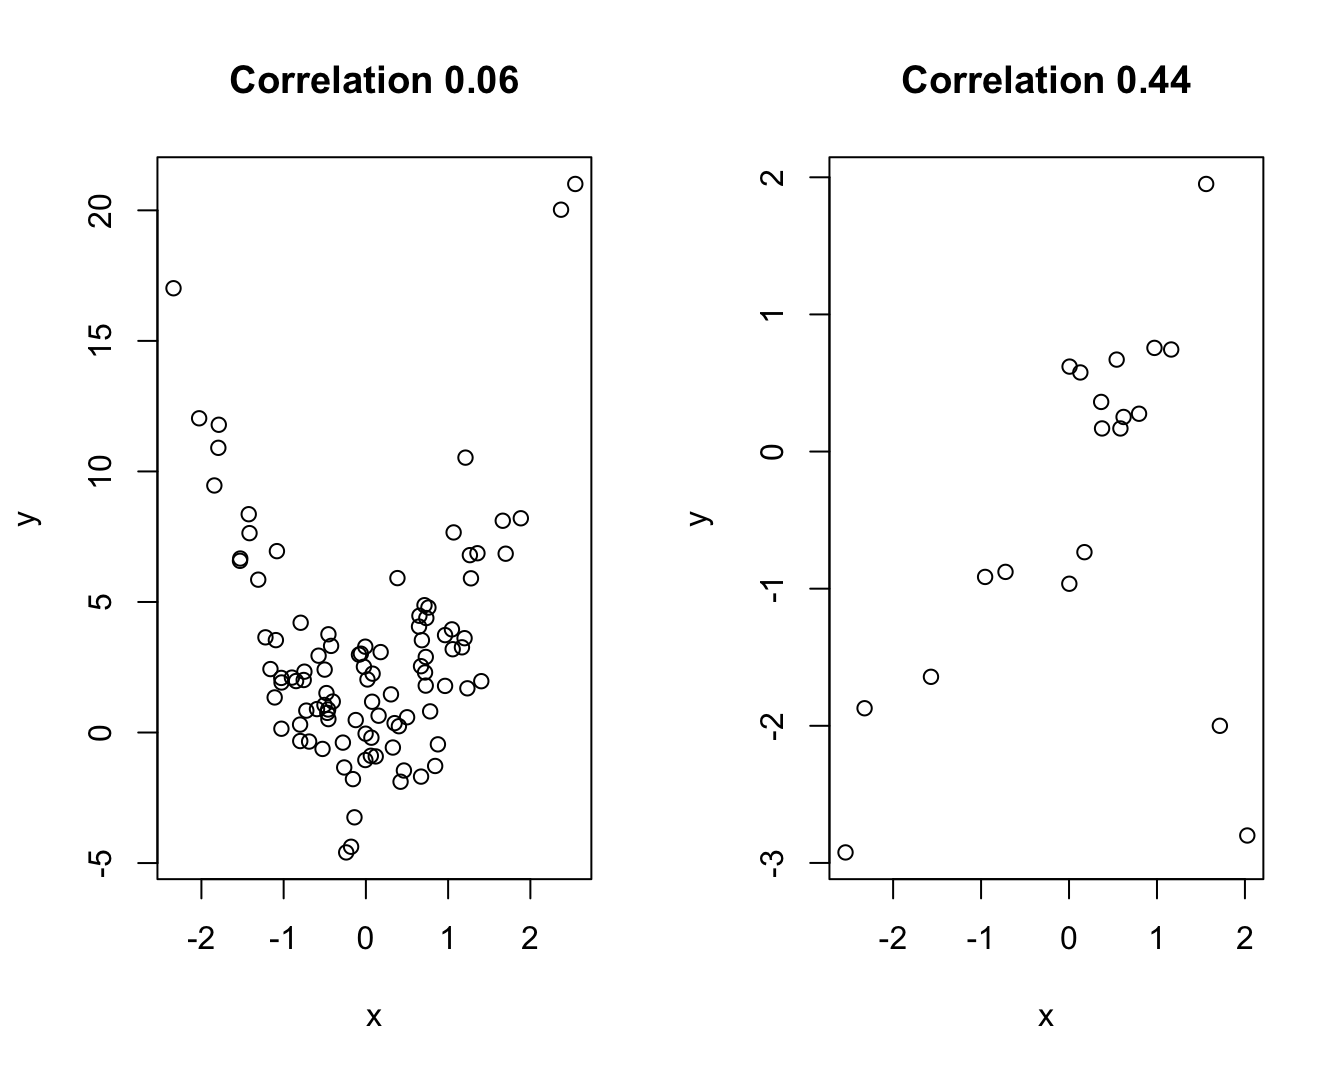
\includegraphics[width=1\linewidth]{Statistiek_2019_2020_files/figure-latex/regr2-1} 

}

\caption{Links: gesimuleerde gegevens met kwadratische associatie; Rechts: gesimuleerde gegevens met een werkelijke correlatie van 0.9 en 2 outliers.}\label{fig:regr2}
\end{figure}

\begin{Shaded}
\begin{Highlighting}[]
\CommentTok{# Met outliers}
\KeywordTok{cor}\NormalTok{(simHlp)}
\end{Highlighting}
\end{Shaded}

\begin{verbatim}
##           [,1]      [,2]
## [1,] 1.0000000 0.4399447
## [2,] 0.4399447 1.0000000
\end{verbatim}

\begin{Shaded}
\begin{Highlighting}[]
\CommentTok{# Zonder outliers}
\KeywordTok{cor}\NormalTok{(simHlp[}\DecValTok{1}\OperatorTok{:}\DecValTok{18}\NormalTok{, ])}
\end{Highlighting}
\end{Shaded}

\begin{verbatim}
##           [,1]      [,2]
## [1,] 1.0000000 0.9270999
## [2,] 0.9270999 1.0000000
\end{verbatim}

\begin{enumerate}
\def\labelenumi{\arabic{enumi}.}
\setcounter{enumi}{1}
\tightlist
\item
  Merk op dat een correlatiecoëfficiënt van 0 tussen 2 variabelen \(X\)
  en \(Y\) niet noodzakelijk impliceert dat deze variabelen
  onafhankelijk zijn. Figuur \ref{fig:regr2} (links) toont ter
  bijvoorbeeld 2 variabelen die vrij sterk geassocieerd zijn, hoewel hun
  correlatie nagenoeg 0 bedraagt. De oorzaak hiervan is dat de
  correlatie enkel de lineaire samenhang tussen 2 variabelen meet en
  bijgevolg niet noodzakelijk niet-lineaire verbanden detecteert. Dit
  betekent meer concreet dat de correlatie, op een factor na, de helling
  weergeeft van de `best passende rechte' (nl. de kleinste
  kwadratenrechte, zie Hoofdstuk \ref{chap:linReg}) doorheen de
  puntenwolk. Een correlatie gelijk aan 0 geeft bijgevolg aan dat een
  best passende rechte doorheen de puntenwolk helling 0 heeft (d.w.z.
  dat ze horizontaal verloopt). In Figuur \ref{fig:regr2} is de
  correlatie heel laag omdat er bij negatieve \(X\)-waarden een dalende
  associatie is en bij positieve \(X\)-waarden een stijgende associatie,
  zodat de 2 variabelen geen lineaire samenhang meer hebben.
\end{enumerate}

Omwille van het voorgaande fenomeen is het van belang om de aard van
samenhang tussen 2 variabelen steeds te onderzoeken via een scatterplot
alvorens een correlatiecoëfficiënt te rapporteren. Wanneer het verband
monotoon is, maar sterk niet-lineair is, dan is het aangewezen om niet
de Pearson correlatiecoëfficiënt, maar Spearman's correlatiecoëfficiënt
te rapporteren.

Figuur \ref{fig:brcaOrigFit} geeft het verband van de microarray
intensiteitsmetingen weer voor het S100A8 gen in functie van deze voor
het ESR1 gen. Het verband is moeilijk interpreteerbaar op de originele
schaal door de aanwezigheid van heel hoge intensiteiten (en dus
concentraties). Het verband op de originele schaal is exponentieel.
Pearson's correlatiecoëfficiënt zakt hierdoor van -0.89 op log-schaal
naar -0.54 op de originele schaal. Spearman's correlatiecoëfficiënt
daarentegen blijft gelijk voor en na transformatie gezien de log2
transformatie monotoon is en de ordening (rangen) van de data niet
verandert. Spearman's correlatiecoëfficiënt blijft -0.73 op de originele
schaal alsook op log-schaal en wijst op een sterke negatieve associatie
tussen de expressie van beiden genen.

\begin{Shaded}
\begin{Highlighting}[]
\KeywordTok{par}\NormalTok{(}\DataTypeTok{mfrow =} \KeywordTok{c}\NormalTok{(}\DecValTok{1}\NormalTok{, }\DecValTok{3}\NormalTok{))}
\KeywordTok{with}\NormalTok{(borstkanker, }\KeywordTok{scatter.smooth}\NormalTok{(}\KeywordTok{log2}\NormalTok{(ESR1), }\KeywordTok{log2}\NormalTok{(S100A8), }
    \DataTypeTok{span =} \DecValTok{1}\OperatorTok{/}\DecValTok{2}\NormalTok{, }\DataTypeTok{main =} \KeywordTok{paste}\NormalTok{(}\StringTok{"Correlatie"}\NormalTok{, }\KeywordTok{c}\NormalTok{(}\StringTok{"Pearson"}\NormalTok{, }
        \StringTok{"Spearman"}\NormalTok{), }\KeywordTok{round}\NormalTok{(}\KeywordTok{c}\NormalTok{(}\KeywordTok{cor}\NormalTok{(}\KeywordTok{log2}\NormalTok{(ESR1), }\KeywordTok{log2}\NormalTok{(S100A8)), }
        \KeywordTok{cor}\NormalTok{(}\KeywordTok{log2}\NormalTok{(ESR1), }\KeywordTok{log2}\NormalTok{(S100A8), }\DataTypeTok{method =} \StringTok{"spearman"}\NormalTok{)), }
        \DecValTok{2}\NormalTok{))))}
\KeywordTok{with}\NormalTok{(borstkanker, }\KeywordTok{scatter.smooth}\NormalTok{(ESR1, S100A8, }\DataTypeTok{span =} \DecValTok{1}\OperatorTok{/}\DecValTok{2}\NormalTok{, }
    \DataTypeTok{main =} \KeywordTok{paste}\NormalTok{(}\StringTok{"Correlatie"}\NormalTok{, }\KeywordTok{c}\NormalTok{(}\StringTok{"Pearson"}\NormalTok{, }\StringTok{"Spearman"}\NormalTok{), }
        \KeywordTok{round}\NormalTok{(}\KeywordTok{c}\NormalTok{(}\KeywordTok{cor}\NormalTok{(ESR1, S100A8), }\KeywordTok{cor}\NormalTok{(ESR1, S100A8, }
            \DataTypeTok{method =} \StringTok{"spearman"}\NormalTok{)), }\DecValTok{2}\NormalTok{))))}
\KeywordTok{with}\NormalTok{(borstkanker, }\KeywordTok{scatter.smooth}\NormalTok{(ESR1, S100A8, }\DataTypeTok{span =} \DecValTok{1}\OperatorTok{/}\DecValTok{2}\NormalTok{, }
    \DataTypeTok{ylim =} \KeywordTok{c}\NormalTok{(}\DecValTok{0}\NormalTok{, }\DecValTok{500}\NormalTok{), }\DataTypeTok{main =} \KeywordTok{paste}\NormalTok{(}\StringTok{"Correlatie"}\NormalTok{, }\KeywordTok{c}\NormalTok{(}\StringTok{"Pearson"}\NormalTok{, }
        \StringTok{"Spearman"}\NormalTok{), }\KeywordTok{round}\NormalTok{(}\KeywordTok{c}\NormalTok{(}\KeywordTok{cor}\NormalTok{(ESR1, S100A8), }\KeywordTok{cor}\NormalTok{(ESR1, }
\NormalTok{        S100A8, }\DataTypeTok{method =} \StringTok{"spearman"}\NormalTok{)), }\DecValTok{2}\NormalTok{))))}
\end{Highlighting}
\end{Shaded}

\begin{figure}

{\centering 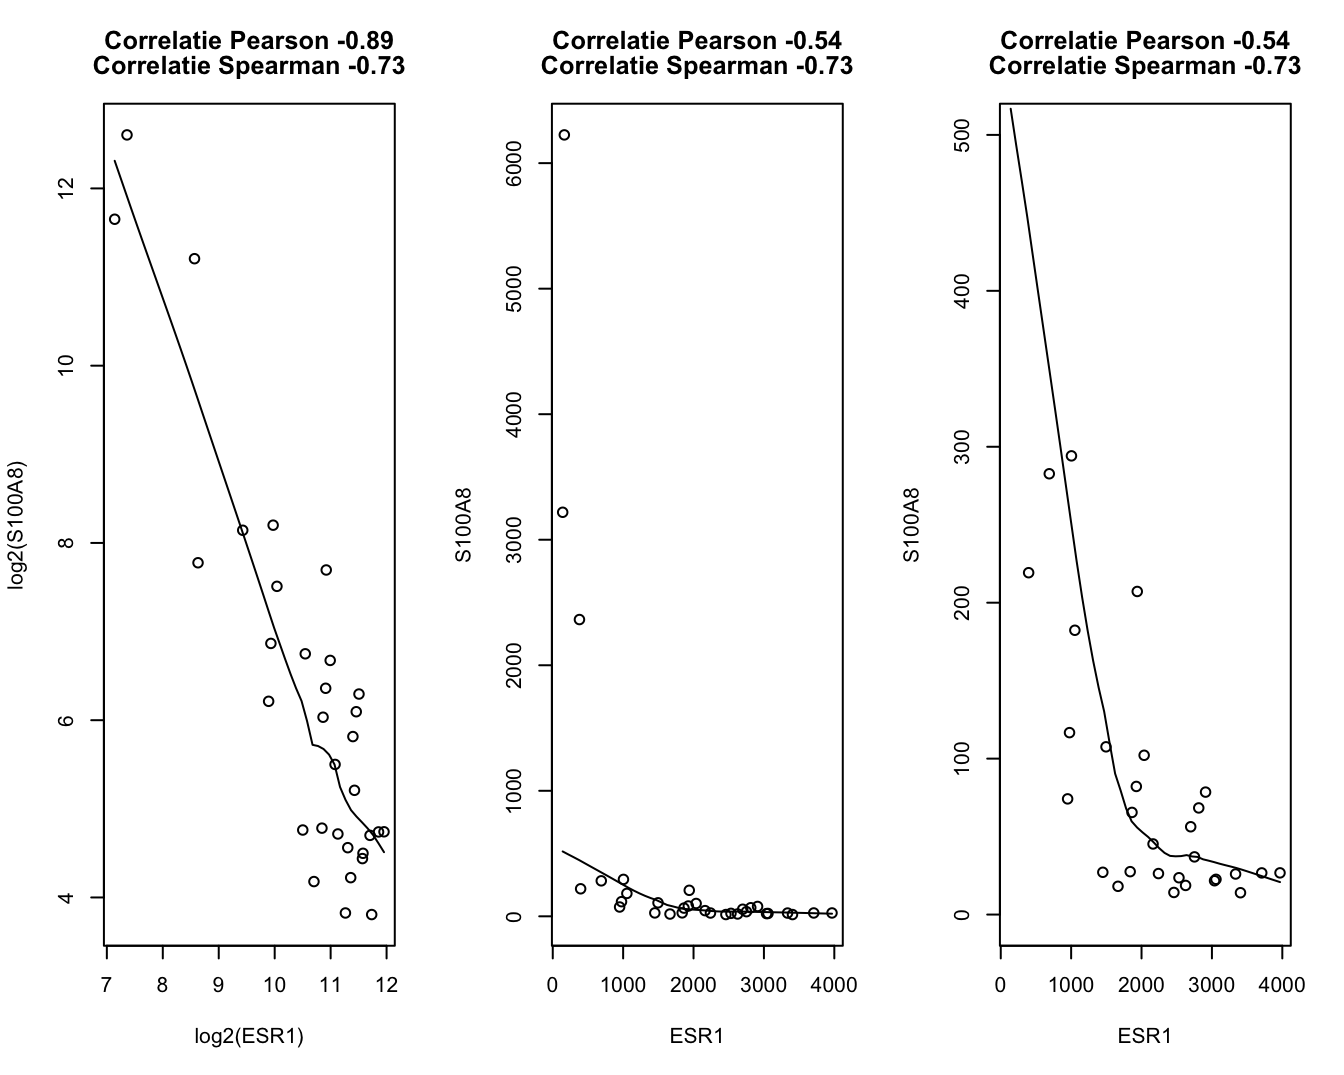
\includegraphics[width=1\linewidth]{Statistiek_2019_2020_files/figure-latex/brcaOrigFit-1} 

}

\caption{Expressie van het S100A8 gen in functie van de ESR1 gen-expressie op de log2 en originele schaal.}\label{fig:brcaOrigFit}
\end{figure}

Indien het verband niet-monotoon is, dan zijn correlatiecoëfficiënten
niet geschikt en moet men overstappen op meer geavanceerde
regressietechnieken.

\begin{enumerate}
\def\labelenumi{\arabic{enumi}.}
\setcounter{enumi}{2}
\tightlist
\item
  Bij jonge kinderen is de grootte van hun schoenmaat uiteraard sterk
  gecorreleerd met hun leescapaciteiten. Dat op zich impliceert echter
  niet dat het leren van nieuwe woorden hun voeten doet groeien of dat
  het groeien van hun voeten impliceert dat ze beter kunnen lezen. Ook
  algemeen\footnote{In het Engels is dit welbekend onder de zinsnede
    \emph{`Association is not causation!'}.} hoeft een correlatie tussen
  2 variabelen niet te impliceren dat er een causaal verband is. De
  relatie tussen 2 metingen kan immers sterk verstoord worden door
  confounders (bvb. de leeftijd in bovenstaand voorbeeld). Hoewel dit
  overduidelijk is in bovenstaand voorbeeld, is het in vele andere
  contexten veel minder duidelijk en worden er, vooral in de populaire
  literatuur, vaak causale beweringen gemaakt die niet (volledig) door
  de gegevens worden gestaafd. Volgend voorbeeld illustreert dit.
\end{enumerate}

\BeginKnitrBlock{example}[Associatie versus causatie]
\protect\hypertarget{exm:unnamed-chunk-61}{}{\label{exm:unnamed-chunk-61}
\iffalse (Associatie versus causatie) \fi{} }
\EndKnitrBlock{example}

Wanneer men de incidentie van sterfte ten gevolge van borstkanker uitzet
t.o.v. van de vetinname per capita per dag voor een grote steekproef van
landen over de ganse wereld, dan stelt men vast dat er sterke positieve
correlatie is. Deze correlatie wordt vaak gebruikt om aan te geven dat
vetinname leidt tot borstkanker (analoog voor darmkanker). Het bewijs
hiervoor is echter zeer zwak. Immers, landen met een grote vetinname
hebben ook een hoge inname van suiker. Een grafiek van de incidentie van
sterfte ten gevolge van borstkanker t.o.v. van de suikerinname per
capita per dag toont een vrijwel even sterke correlatie, hoewel nagenoeg
niemand beweert dat suiker borstkanker veroorzaakt. Bovendien zijn vet
en suiker op wereldschaal relatief dure producten. Landen met hoge
vetinname zijn bijgevolg voornamelijk industrielanden die in heel wat
meer verschillen van de andere landen dan alleen hun vetinname\ldots{}
Recente studies (Holmes et al., 1999) hebben intussen sterke indicaties
geleverd dat hoog vetverbruik vermoedelijk niet tot borstkanker leidt.

\texttt{**Einde\ voorbeeld**}

\begin{enumerate}
\def\labelenumi{\arabic{enumi}.}
\setcounter{enumi}{3}
\tightlist
\item
  Een \emph{ecologische analyse} is een statistische analyse waarbij men
  associaties bestudeert tussen samenvattingsmaten (zoals gemiddelden,
  incidenties, \ldots{}) die reeds berekend werden voor groepen
  subjecten. Dit is het geval in voorgaand voorbeeld waar de associatie
  wordt onderzocht tussen de incidentie van sterfte t.g.v. borstkanker
  en de (gemiddelde) dagelijkse vetinname per capita in verschillende
  landen. Wanneer men aldus een \emph{ecologische correlatie} vaststelt
  voor groepen subjecten of individuen (in dit geval, landen),
  impliceert dat niet noodzakelijk dat deze correlatie ook voor de
  subjecten zelf opgaat\footnote{In het Engels is dit welbekend onder de
    naam \emph{`ecological fallacy'}.}. Volgend voorbeeld illustreert
  dit.
\end{enumerate}

\BeginKnitrBlock{example}[Ecological fallacy]
\protect\hypertarget{exm:unnamed-chunk-62}{}{\label{exm:unnamed-chunk-62}
\iffalse (Ecological fallacy) \fi{} }
\EndKnitrBlock{example}

Voor de 48 staten in de V.S. werden telkens 2 getallen berekend: het
percentage van de mensen die in een ander land geboren zijn en het
percentage geletterden. De correlatie ertussen bedraagt 0.53 (Robinson,
1950). Dit is een \emph{ecologische correlatie} omdat de eenheid van de
analyse de groep residenten uit een zelfde staat is, en niet de
individuele residenten zelf. Deze ecologische correlatie suggereert dat
mensen van vreemde afkomst doorgaans beter geschoold zijn (in Amerikaans
Engels) dan de oorspronkelijke inwoners. Wanneer men echter de
correlatie berekent op basis van de gegevens voor alle individuele
residenten, bekomt men -0.11. De ecologische analyse is hier duidelijk
misleidend: het teken van de correlatie is er positief omdat mensen van
vreemde origine de neiging hebben om te gaan wonen in staten waar de
oorspronkelijke bevolking relatief goed geschoold is.

\texttt{**Einde\ voorbeeld**}

\section{Onvolledige gegevens}\label{sec:missing}

Het gebeurt vaak in de biowetenschappen dat, ondanks zorgvuldig veld- en
laboratoriumwerk, metingen die men plande te verzamelen, niet bekomen
werden. Men noemt deze dan \emph{ontbrekende gegevens} of \emph{missing
data (points)}.

Minder drastisch, kunnen observaties soms slechts ten dele gekend zijn.
Bijvoorbeeld bij een studie van de overlevingsduur van dieren en planten
wacht men niet steeds tot alle subjecten gestorven zijn. Op het eind van
de studie zal men bijvoorbeeld voor een 50-jarige olifant die in leven
is, slechts weten dat de overlevingstijd minstens 50 jaar bedraagt, maar
niet de exacte waarde kennen. Zo'n gegeven wordt
\emph{rechts-gecensureerd} genoemd: we weten dat de gewenste observatie
rechts van 50 ligt, maar verder niets meer.

Analoog kunnen observaties \emph{links-gecensureerd} zijn. Bij het meten
van bepaalde concentraties kan een detectielimiet bestaan: een
ondergrens beneden dewelke het meettoestel geen aanwezigheid kan
detecteren. Men weet in zo'n geval dat de concentratie kleiner dan die
ondergrens is, maar niet hoeveel kleiner.

Tenslotte vermelden we nog \emph{interval-gecensureerde} gegevens. Bij
het screenen naar HIV bijvoorbeeld, zal men weten dat een subject
seropositief geworden is ergens tussen de laatste negatieve HIV test en
de eerste positieve HIV test, maar het exacte tijdstip van seroconversie
blijft onbekend.

De aanwezigheid van gegevens die niet of slechts partieel zijn opgemeten
zorgt altijd voor extra moeilijkheden bij de analyse en interpretatie
van de onderzoeksresultaten. Dat is omdat de missende gegevens mogelijks
afkomstig zijn van een speciale populatie. Dat is het meest duidelijk in
klinische experimenten bij mensen. Patiënten zullen hier vaak de studie
verlaten wanneer ze genezen zijn, in welk geval men de metingen van deze
patiënten niet te zien krijgt. Dit negeren door enkel de aanwezige
gegevens te analyseren, zal de resultaten er slechter doen uitzien dan
ze in werkelijkheid zijn. Meestal houdt dat immers de veronderstelling
in dat de aanwezige gegevens representatief blijven voor de populatie
die men wenst te bestuderen. Dit kan in sommige gevallen de resultaten
sterk vertekenen. In de statistische literatuur zijn de laatste jaren
heel wat complexe technieken ontwikkeld om hiervoor te corrigeren. Deze
technieken worden meer en meer in de statistische software ingebouwd en
recent heeft ook R verschillende bibliotheken toegevoegd. Het is echter
aangewezen om voor het gebruik van deze gevorderde technieken een
statisticus te consulteren.

\chapter{Statistische besluitvorming}\label{chap:besluit}

\section{Inleiding}\label{inleiding-3}

In dit hoofdstuk zullen we werken rond de \emph{Captopril dataset}.
Captopril is een medicijn dat wordt voorgeschreven bij hypertensie en
chronisch hartfalen. Het behoort tot de klasse van ACE remmers die
activiteit van het renine-angiotensine-aldosteronsysteem onderdrukken.
Dat systeem zet het hormoon angiotensineI om in angiotensine II, die een
krachtige vaatvernauwende werking heeft. ACE remmers verminderen de
omzetting van angiotensine I naar angiotensine II waardoor de
vaatvernauwing wordt onderdrukt. Tijdens de ontwikkeling van het
medicijn werd een eerste kleine studie opgezet om na te gaan of
captopril een bloeddrukverlagend effect heeft bij patiënten met
hypertensie.

Observaties bij een klein aantal subjecten mogen een onderzoeker er dan
al van overtuigen iets nieuws te hebben ontdekt, maar om anderen te
overtuigen zijn objectieve, wetenschappelijke argumenten nodig.
Vooreerst moeten de resultaten voldoende \emph{representatief} zijn,
d.w.z. veralgemeenbaar naar een ruime biologische populatie (bvb. naar
de volledige populatie van patiënten met hypertensie). Ten tweede moet
er rekening mee gehouden worden dat de resultaten \emph{variabel} zijn,
d.w.z. dat men door toeval doorgaans andere resultaten zou vinden indien
men een andere, vergelijkbare groep subjecten zou analyseren. Om die
reden is het belangrijk om uit te drukken in welke mate de resultaten
(bvb. de geschatte bloeddrukdaling) zouden variëren van steekproef tot
steekproef en of men op basis van de steekproef kan aantonen dat er een
effect is van een behandeling (b.v. dat het middel captopril
bloeddrukverlagend werkt in de populatie). Dit vormt het doel van dit
hoofdstuk.

Om een representatieve groep subjecten te waarborgen, vertrekt een goede
onderzoeksopzet vanuit een belangrijke, precies geformuleerde
vraagstelling omtrent een duidelijk omschreven populatie.

Zoals eerder in de cursus aangegeven, zal men in de praktijk om
financiële en logistieke redenen bijna nooit een volledige populatie
kunnen bestuderen. Populatieparameters kunnen daarom meestal niet exact
bepaald worden. Enkel een deel van de populatie kan onderzocht worden,
wat men een \emph{steekproef} noemt. Volgens een gestructureerd design
worden daartoe lukraak subjecten uit de doelpopulatie getrokken en
geobserveerd. De onbekende parameters worden vervolgens geschat o.b.v.
die steekproef en noemt men schattingen. In de praktijk hoopt men
uiteraard dat de schattingen die men bekomt op basis van de steekproef
vergelijkbaar zijn met de overeenkomstige populatieparameters die men
voor de volledige populatie zou bekomen.\\
Typisch kan de onderzoeksvraag worden vertaald naar een
populatieparameter. Ze kan bijvoorbeeld worden uitgedrukt in termen van
een populatiegemiddelde, bijvoorbeeld de gemiddelde bloeddrukverandering
na de inname van captopril bij patiënten met hypertensie.

\section{Captopril voorbeeld}\label{captopril-voorbeeld}

Onderzoekers wensen na te gaan of het medicijn Captopril een bloeddruk
verlagend effect heeft. De onderzoekers wensen uitspraken te kunnen doen
over het effect van captopril op de systolische bloeddruk van huidige en
toekomstige patiënten met hypertensie, m.a.w. ze wensen uitspraken te
doen over het effect van captopril op het niveau van de
\emph{Populatie}. Ze zullen hiervoor een experiment opzetten om het
effect van captopril bestuderen (\emph{Proefopzet}) waarbij een
\emph{steekproef} (sample) van de patiënten met hypertensie is getrokken
uit de populatie. Vervolgens zullen ze de data exploreren en het effect
van captopril besturen in de steekproef (\emph{Data Exploratie \&
Beschrijvende Statistiek}). Op basis van de steekproef zullen ze dan het
effect van captopril \emph{Schatten} in de populatie en zullen ze
a.d.h.v. methoden uit \emph{Statistische besluitvorming}\footnote{Ook
  wel Statistische Inferentie genoemd} nagaan in hoeverre de
geobserveerde effecten in de steekproef veralgemeend kunnen worden naar
de algemene populatie toe.

Deze verschillende stappen worden geïllustreerd in Figuur
\ref{fig:captoPop2Samp2Pop}.

\begin{figure}

{\centering 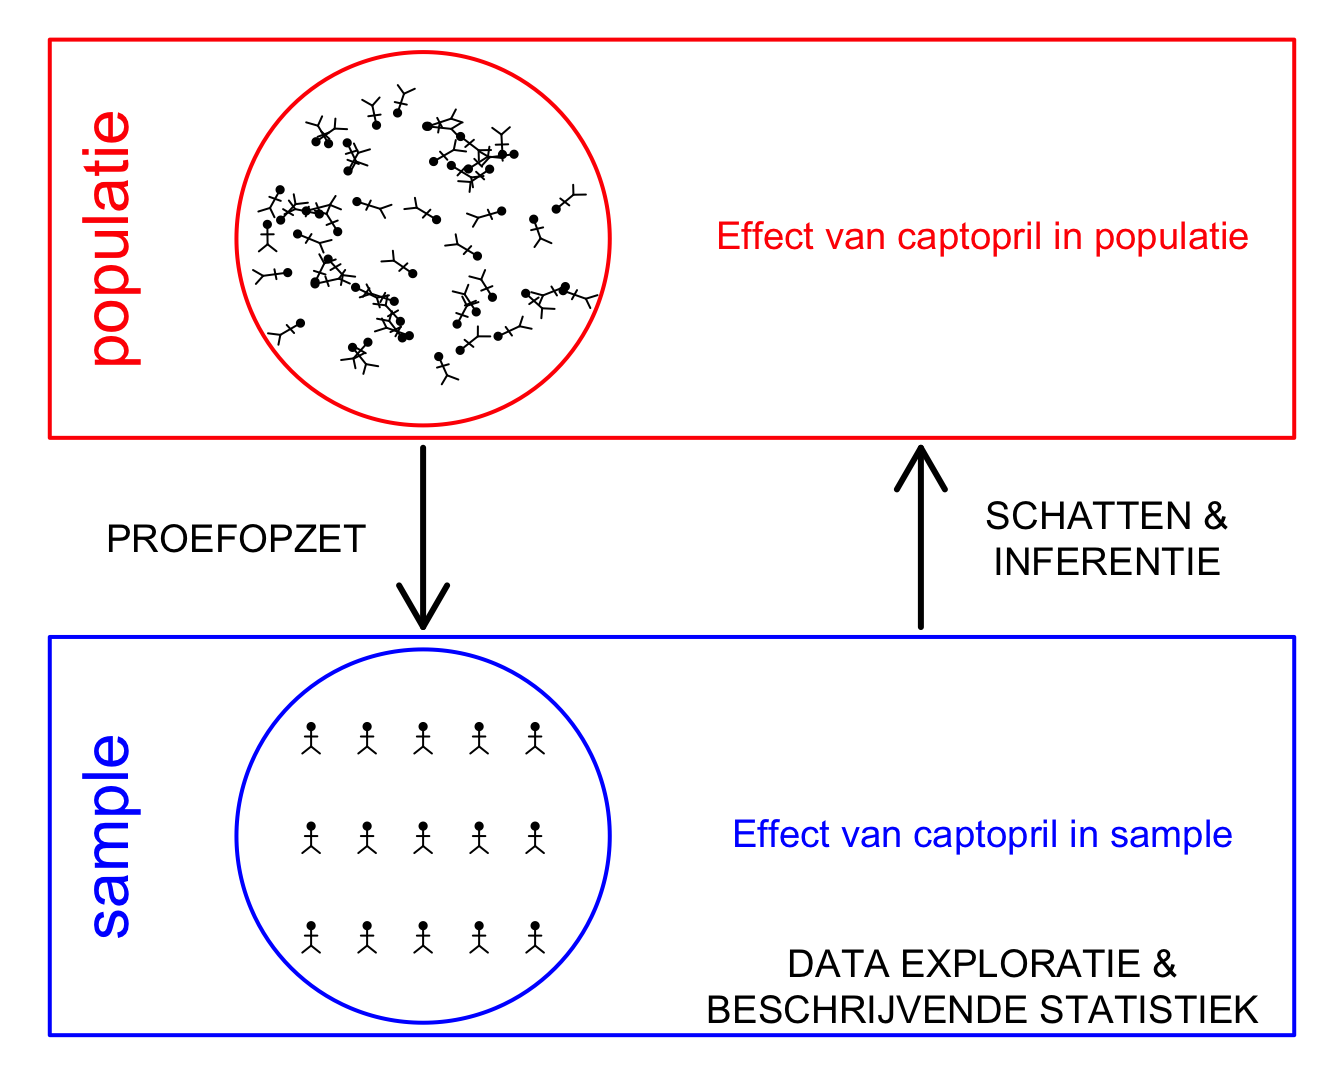
\includegraphics[width=1\linewidth]{Statistiek_2019_2020_files/figure-latex/captoPop2Samp2Pop-1} 

}

\caption{Verschillende stappen in de captopril studie.}\label{fig:captoPop2Samp2Pop}
\end{figure}

\subsection{Proefopzet}\label{proefopzet}

Bij proefopzet zullen we een gestructureerd design voorstellen om
lukraak subjecten uit de doelpopulatie te selecteren, toe te wijzen aan
een behandeling en te observeren. We zullen hierbij een response
variabele meten, een karakteristiek van interesse. In het captopril
voorbeeld is dit de systolische bloeddruk.

In de captopril studie hebben de onderzoekers gebruik gemaakt van een
een pre-test/post-test design. De patiënten werden at random gekozen uit
de populatie. Van elke patiënt in de studie werd de systolische en
diasystolische bloeddruk gemeten voor en na het toedienen van captopril.
Het pre-test/post-test design heeft als voordeel dat we het effect van
het toedienen van captopril op de bloeddruk kunnen meten voor elke
patiënt. Een nadeel daarentegen is dat er geen controle behandeling is
waardoor we een mogelijkse bloeddrukverlaging niet noodzakelijkerwijs
kunnen toeschrijven aan de werking van captopril. Er zou immers ook een
placebo-effect kunnen optreden waardoor de bloeddruk van de patiënt
daalt omdat men weet dat men een medicijn kreeg tegen een hoge
bloeddruk.

\subsection{Data Exploratie \& Beschrijvende
Statistiek}\label{data-exploratie-beschrijvende-statistiek}

Eens de data zijn geobserveerd, is het belangrijk om deze te exploreren
om inzicht te krijgen in hun verdeling en karakteristieken. Vervolgens
zullen we de gegevens samenvatten zodat we het effect van interesse
kunnen kwantificeren in de steekproef. In deze studie is de systolische
bloeddruk en de diasystolische bloeddruk gemeten voor elke patiënt voor
en na het toedienen van captopril. De data is opgeslagen in een
tekstbestand met naam \texttt{captopril.txt} in de folder dataset. We
zullen eerst exploreren welke figuren nuttig zijn in onze context. In
wetenschappelijke artikels worden vaak figuren gemaakt van het
gemiddelde en de standaardafwijking (zie Figuur \ref{fig:captoBar}).

\begin{Shaded}
\begin{Highlighting}[]
\CommentTok{# Eerst lezen we de data in.  Deze bevindt zich in}
\CommentTok{# de subdirectory dataset Het is een tekstbestand}
\CommentTok{# waarbij de kolommen van elkaar gescheiden zijn}
\CommentTok{# d.m.v kommas. sep=',' De eerste rij bevat de}
\CommentTok{# namen van de variabelen}
\NormalTok{captopril <-}\StringTok{ }\KeywordTok{read.table}\NormalTok{(}\StringTok{"dataset/captopril.txt"}\NormalTok{, }\DataTypeTok{header =} \OtherTok{TRUE}\NormalTok{, }
    \DataTypeTok{sep =} \StringTok{","}\NormalTok{)}
\KeywordTok{head}\NormalTok{(captopril)}
\end{Highlighting}
\end{Shaded}

\begin{verbatim}
##   id SBPb DBPb SBPa DBPa
## 1  1  210  130  201  125
## 2  2  169  122  165  121
## 3  3  187  124  166  121
## 4  4  160  104  157  106
## 5  5  167  112  147  101
## 6  6  176  101  145   85
\end{verbatim}

\begin{Shaded}
\begin{Highlighting}[]
\CommentTok{# We gebruiken de apply functie om het gemiddelde}
\CommentTok{# en de standaard deviatie te berekenen voor de}
\CommentTok{# kolommen die bloeddruk data bevatten (kolom 2:4)}
\CommentTok{# We gebruiken argument MARGIN=2 om de functie toe}
\CommentTok{# te passen op de kolommen MARGIN=1 kan gebruikt}
\CommentTok{# worden om de functie op de rijen toe te passen}
\NormalTok{mm <-}\StringTok{ }\KeywordTok{apply}\NormalTok{(captopril[, }\DecValTok{2}\OperatorTok{:}\DecValTok{5}\NormalTok{], }\DataTypeTok{MARGIN =} \DecValTok{2}\NormalTok{, }\DataTypeTok{FUN =}\NormalTok{ mean)}
\NormalTok{hh <-}\StringTok{ }\KeywordTok{apply}\NormalTok{(captopril[, }\DecValTok{2}\OperatorTok{:}\DecValTok{5}\NormalTok{], }\DataTypeTok{MARGIN =} \DecValTok{2}\NormalTok{, }\DataTypeTok{FUN =}\NormalTok{ sd)}

\NormalTok{mp <-}\StringTok{ }\KeywordTok{barplot}\NormalTok{(mm, }\DataTypeTok{ylim =} \KeywordTok{c}\NormalTok{(}\DecValTok{0}\NormalTok{, }\DecValTok{250}\NormalTok{), }\DataTypeTok{ylab =} \StringTok{"Gemiddelde bloeddruk (mmHg)"}\NormalTok{, }
    \DataTypeTok{main =} \StringTok{""}\NormalTok{)}
\CommentTok{# fouten vlaggen}
\KeywordTok{segments}\NormalTok{(mp, mm, mp, mm }\OperatorTok{+}\StringTok{ }\DecValTok{2} \OperatorTok{*}\StringTok{ }\NormalTok{hh)}
\KeywordTok{segments}\NormalTok{(mp }\OperatorTok{-}\StringTok{ }\FloatTok{0.2}\NormalTok{, mm }\OperatorTok{+}\StringTok{ }\DecValTok{2} \OperatorTok{*}\StringTok{ }\NormalTok{hh, mp }\OperatorTok{+}\StringTok{ }\FloatTok{0.2}\NormalTok{, mm }\OperatorTok{+}\StringTok{ }\DecValTok{2} \OperatorTok{*}\StringTok{ }
\StringTok{    }\NormalTok{hh)}
\end{Highlighting}
\end{Shaded}

\begin{figure}

{\centering 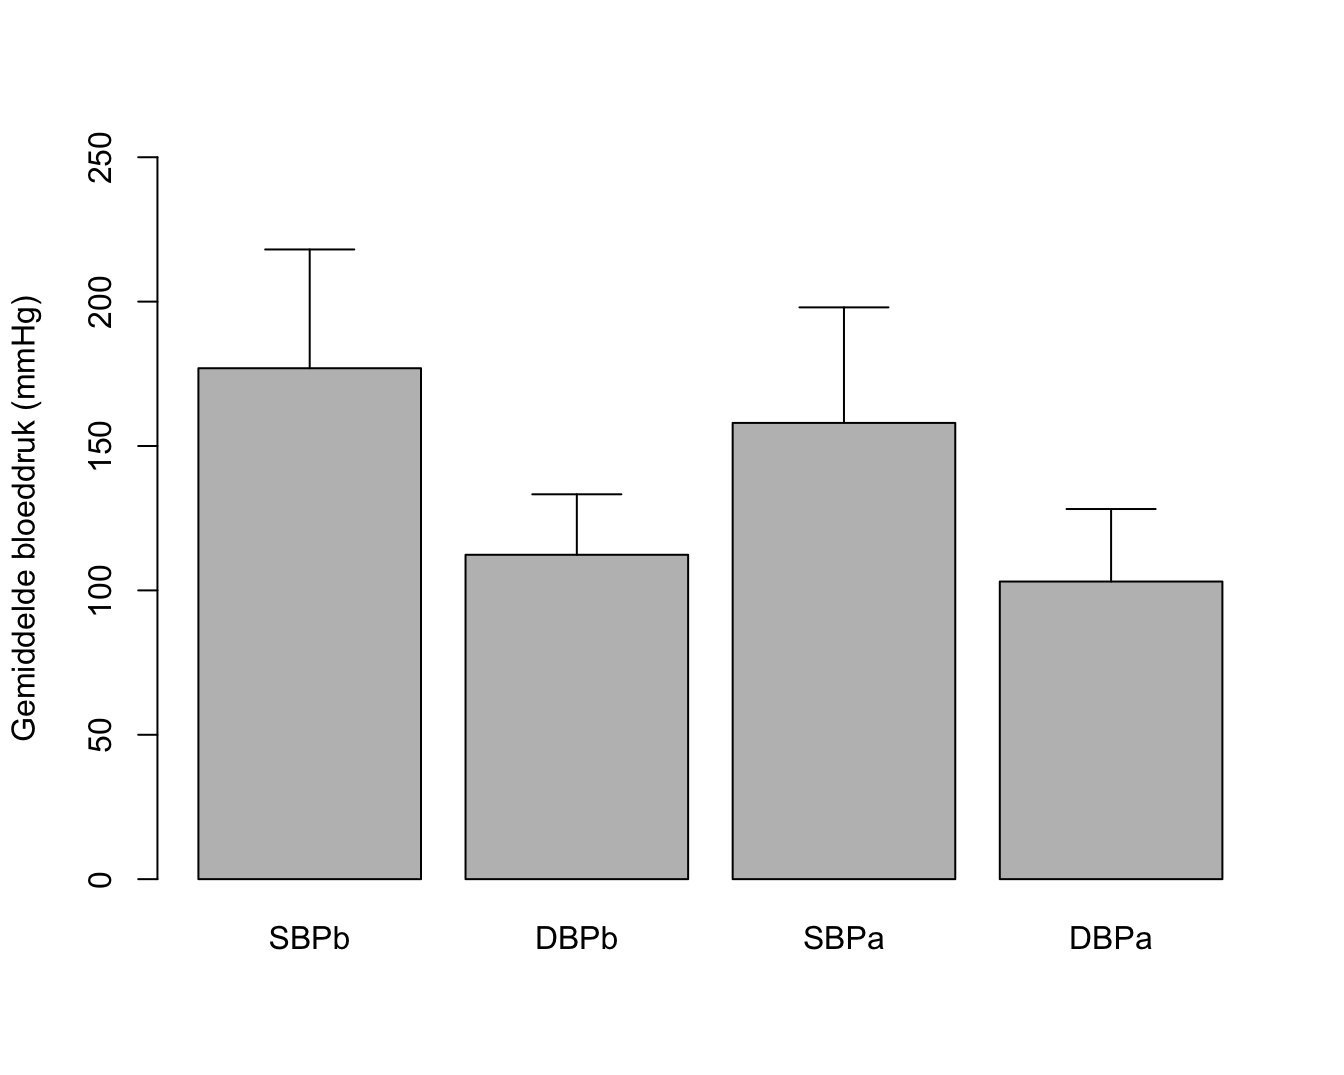
\includegraphics[width=1\linewidth]{Statistiek_2019_2020_files/figure-latex/captoBar-1} 

}

\caption{Barplot van de gemiddelde bloeddruk in de captopril studie. De foutenvlag is 2x de standaard deviatie op de metingen (SBPb: systolic BloodPressure before, DBPb: Diasystolic BloodPressure before, SBPa: systolic BloodPressure after, DBPa: Diasystolic BloodPressure after).}\label{fig:captoBar}
\end{figure}

De figuur is echter niet informatief. De hoogte van de balken zegt enkel
iets over het gemiddelde. We kunnen onmogelijk weten wat het bereik van
de ruwe gegevens is bijvoorbeeld. Daarom is het beter om de gegevens zo
ruw mogelijk weer te geven in een plot. We kunnen hiervoor bijvoorbeeld
gebruik maken van boxplots (Figuur \ref{fig:captoBox}). Aangezien we
maar over 15 patiënten beschikken kunnen we ook de ruwe datapunten
toevoegen. In de figuur zien we dat de systolische bloeddruk in de
steekproef gemiddeld lager ligt na de behandeling met captopril. We
krijgen ook een duidelijk beeld op het bereik van de data.

\begin{Shaded}
\begin{Highlighting}[]
\KeywordTok{boxplot}\NormalTok{(captopril[, }\DecValTok{2}\OperatorTok{:}\DecValTok{5}\NormalTok{], }\DataTypeTok{ylim =} \KeywordTok{c}\NormalTok{(}\DecValTok{0}\NormalTok{, }\DecValTok{250}\NormalTok{), }\DataTypeTok{ylab =} \StringTok{"Bloeddruk (mmHg)"}\NormalTok{, }
    \DataTypeTok{main =} \StringTok{""}\NormalTok{)}
\CommentTok{# toevoegen van originele datapunten op de plot}
\CommentTok{# jitter zal de punten random verspreiden set seed}
\CommentTok{# om gekleurde volle bol pch=19 te zetten en daarna}
\CommentTok{# een zwarte rand te kunnen zetten op zelfde}
\CommentTok{# plaats.}
\KeywordTok{set.seed}\NormalTok{(}\DecValTok{19}\NormalTok{)}
\KeywordTok{stripchart}\NormalTok{(captopril[, }\DecValTok{2}\OperatorTok{:}\DecValTok{5}\NormalTok{], }\DataTypeTok{vertical =} \OtherTok{TRUE}\NormalTok{, }\DataTypeTok{method =} \StringTok{"jitter"}\NormalTok{, }
    \DataTypeTok{pch =} \DecValTok{19}\NormalTok{, }\DataTypeTok{col =} \KeywordTok{c}\NormalTok{(}\StringTok{"bisque"}\NormalTok{, }\StringTok{"coral"}\NormalTok{, }\StringTok{"darkcyan"}\NormalTok{, }
        \StringTok{"purple"}\NormalTok{), }\DataTypeTok{add =} \OtherTok{TRUE}\NormalTok{)}
\KeywordTok{set.seed}\NormalTok{(}\DecValTok{19}\NormalTok{)}
\KeywordTok{stripchart}\NormalTok{(captopril[, }\DecValTok{2}\OperatorTok{:}\DecValTok{5}\NormalTok{], }\DataTypeTok{vertical =} \OtherTok{TRUE}\NormalTok{, }\DataTypeTok{method =} \StringTok{"jitter"}\NormalTok{, }
    \DataTypeTok{pch =} \DecValTok{1}\NormalTok{, }\DataTypeTok{col =} \DecValTok{1}\NormalTok{, }\DataTypeTok{add =} \OtherTok{TRUE}\NormalTok{)}
\end{Highlighting}
\end{Shaded}

\begin{figure}

{\centering 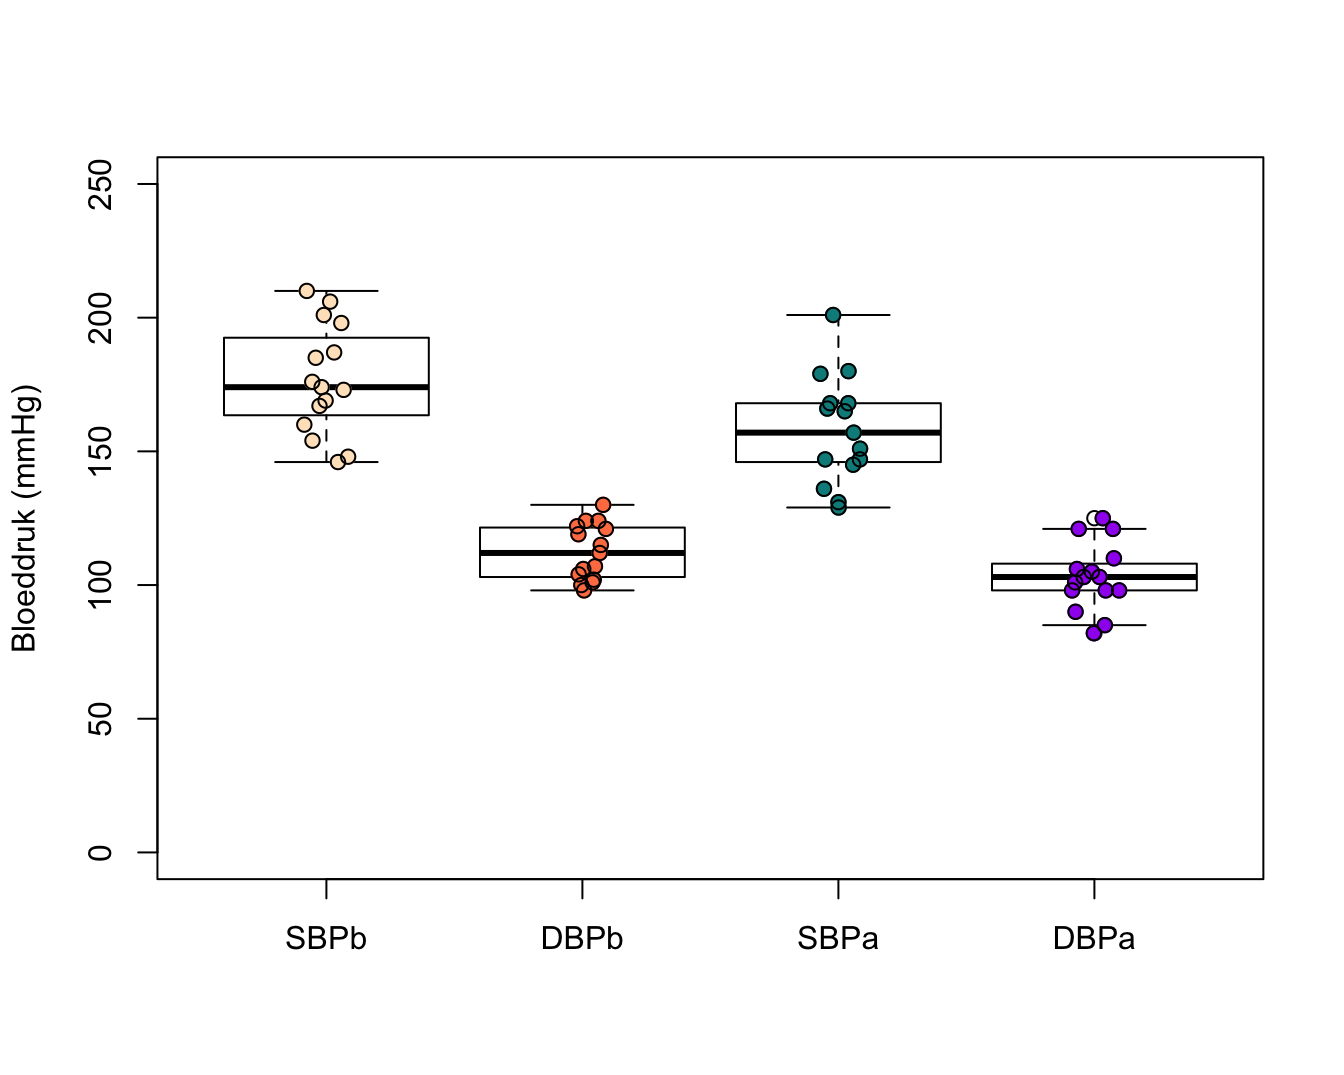
\includegraphics[width=1\linewidth]{Statistiek_2019_2020_files/figure-latex/captoBox-1} 

}

\caption{Boxplot en ruwe data van de bloeddruk in de captopril studie (SBPb: systolic BloodPressure before, DBPb: Diasystolic BloodPressure before, SBPa: systolic BloodPressure after, DBPa: Diasystolic BloodPressure after).}\label{fig:captoBox}
\end{figure}

Als alle bloeddrukmetingen onafhankelijk zouden zijn dan is Figuur
\ref{fig:captoBox} een goede figuur om de data te exploreren. We weten
echter dat de metingen voor en na het toedienen van captopril afkomstig
zijn van dezelfde patiënt. We kunnen die informatie toevoegen in een
dotplot zoals we illustreren voor de systolische bloeddruk in Figuur
\ref{fig:captoDotBsl}. In deze figuur zijn de twee bloeddrukmetingen
voor dezelfde persoon verbonden met een lijn. Deze figuur geeft
duidelijk weer dat de bloeddruk daalt voor elke patiënt wat een sterke
aanwijzing is dat er een effect is van het toedienen van captopril op de
systolische bloeddruk.

\begin{Shaded}
\begin{Highlighting}[]
\CommentTok{# D.m.v de matplot functie kunnen we eenvoudig de}
\CommentTok{# data van dezelfde patient (per kolom) vandaar dat}
\CommentTok{# we de dataset transponeren (t(.)) functie en}
\CommentTok{# verbinden a.d.h.v. een lijn. (lty=1) we gebruiken}
\CommentTok{# ook een dezelfde kleur. en gebruiken zowel een}
\CommentTok{# punt als een lijn om de data voor te stellen}
\CommentTok{# type='b'}
\KeywordTok{matplot}\NormalTok{(}\KeywordTok{t}\NormalTok{(captopril[, }\KeywordTok{c}\NormalTok{(}\StringTok{"SBPb"}\NormalTok{, }\StringTok{"SBPa"}\NormalTok{)]), }\DataTypeTok{pch =} \DecValTok{1}\NormalTok{, }
    \DataTypeTok{lty =} \DecValTok{1}\NormalTok{, }\DataTypeTok{col =} \StringTok{"black"}\NormalTok{, }\DataTypeTok{type =} \StringTok{"b"}\NormalTok{, }\DataTypeTok{xaxt =} \StringTok{"none"}\NormalTok{, }
    \DataTypeTok{xlim =} \KeywordTok{c}\NormalTok{(}\FloatTok{0.5}\NormalTok{, }\FloatTok{2.5}\NormalTok{), }\DataTypeTok{ylab =} \StringTok{"Systolische bloeddruk (mmHg)"}\NormalTok{, }
    \DataTypeTok{cex =} \FloatTok{0.5}\NormalTok{)}
\KeywordTok{axis}\NormalTok{(}\DecValTok{1}\NormalTok{, }\KeywordTok{c}\NormalTok{(}\DecValTok{1}\NormalTok{, }\DecValTok{2}\NormalTok{), }\DataTypeTok{labels =} \KeywordTok{c}\NormalTok{(}\StringTok{"voor"}\NormalTok{, }\StringTok{"na"}\NormalTok{))}
\end{Highlighting}
\end{Shaded}

\begin{figure}

{\centering 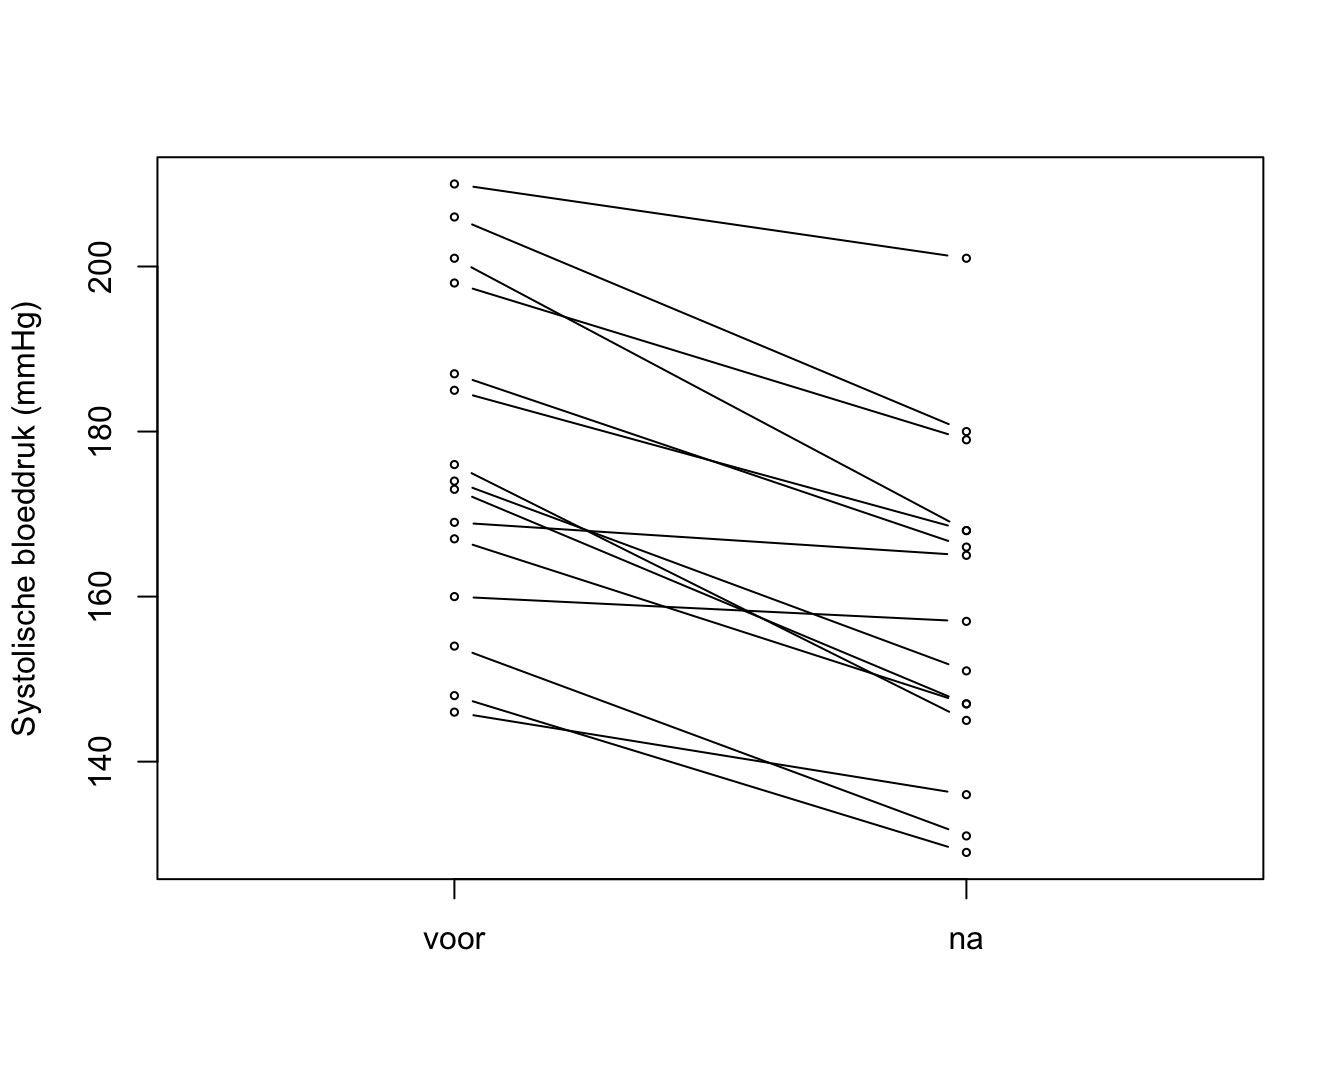
\includegraphics[width=1\linewidth]{Statistiek_2019_2020_files/figure-latex/captoDotBsl-1} 

}

\caption{Dotplot van de systolische bloeddruk in de captopril studie voor en na het toedienen van captopril.}\label{fig:captoDotBsl}
\end{figure}

Aangezien we slechts twee bloeddrukmetingen hebben per patiënt kunnen we
het effect van captopril ook berekenen per patiënt door het verschil in
de systolische bloeddruk na en voor de toediening van captopril te
berekenen. Dat is één van de voordelen van een pre-test/post-test
design.

\begin{Shaded}
\begin{Highlighting}[]
\CommentTok{# we selecteren de bloeddruk na en voor toedienen}
\CommentTok{# uit de dataset via naam van variabele d.m.v.}
\CommentTok{# $-teken en berekenen het verschil}
\NormalTok{delta <-}\StringTok{ }\NormalTok{captopril}\OperatorTok{$}\NormalTok{SBPa }\OperatorTok{-}\StringTok{ }\NormalTok{captopril}\OperatorTok{$}\NormalTok{SBPb}
\KeywordTok{boxplot}\NormalTok{(delta, }\DataTypeTok{ylab =} \KeywordTok{expression}\NormalTok{(}\KeywordTok{paste}\NormalTok{(}\StringTok{"Verschil in bloeddruk ("}\NormalTok{, }
\NormalTok{    Delta[Na }\OperatorTok{-}\StringTok{ }\NormalTok{Voor], }\StringTok{")"}\NormalTok{)))}
\KeywordTok{set.seed}\NormalTok{(}\DecValTok{19}\NormalTok{)}
\KeywordTok{stripchart}\NormalTok{(delta, }\DataTypeTok{vertical =} \OtherTok{TRUE}\NormalTok{, }\DataTypeTok{method =} \StringTok{"jitter"}\NormalTok{, }
    \DataTypeTok{pch =} \DecValTok{19}\NormalTok{, }\DataTypeTok{col =} \KeywordTok{c}\NormalTok{(}\StringTok{"bisque"}\NormalTok{), }\DataTypeTok{add =} \OtherTok{TRUE}\NormalTok{)}
\KeywordTok{set.seed}\NormalTok{(}\DecValTok{19}\NormalTok{)}
\KeywordTok{stripchart}\NormalTok{(delta, }\DataTypeTok{vertical =} \OtherTok{TRUE}\NormalTok{, }\DataTypeTok{method =} \StringTok{"jitter"}\NormalTok{, }
    \DataTypeTok{pch =} \DecValTok{1}\NormalTok{, }\DataTypeTok{col =} \DecValTok{1}\NormalTok{, }\DataTypeTok{add =} \OtherTok{TRUE}\NormalTok{)}
\end{Highlighting}
\end{Shaded}

\begin{figure}

{\centering 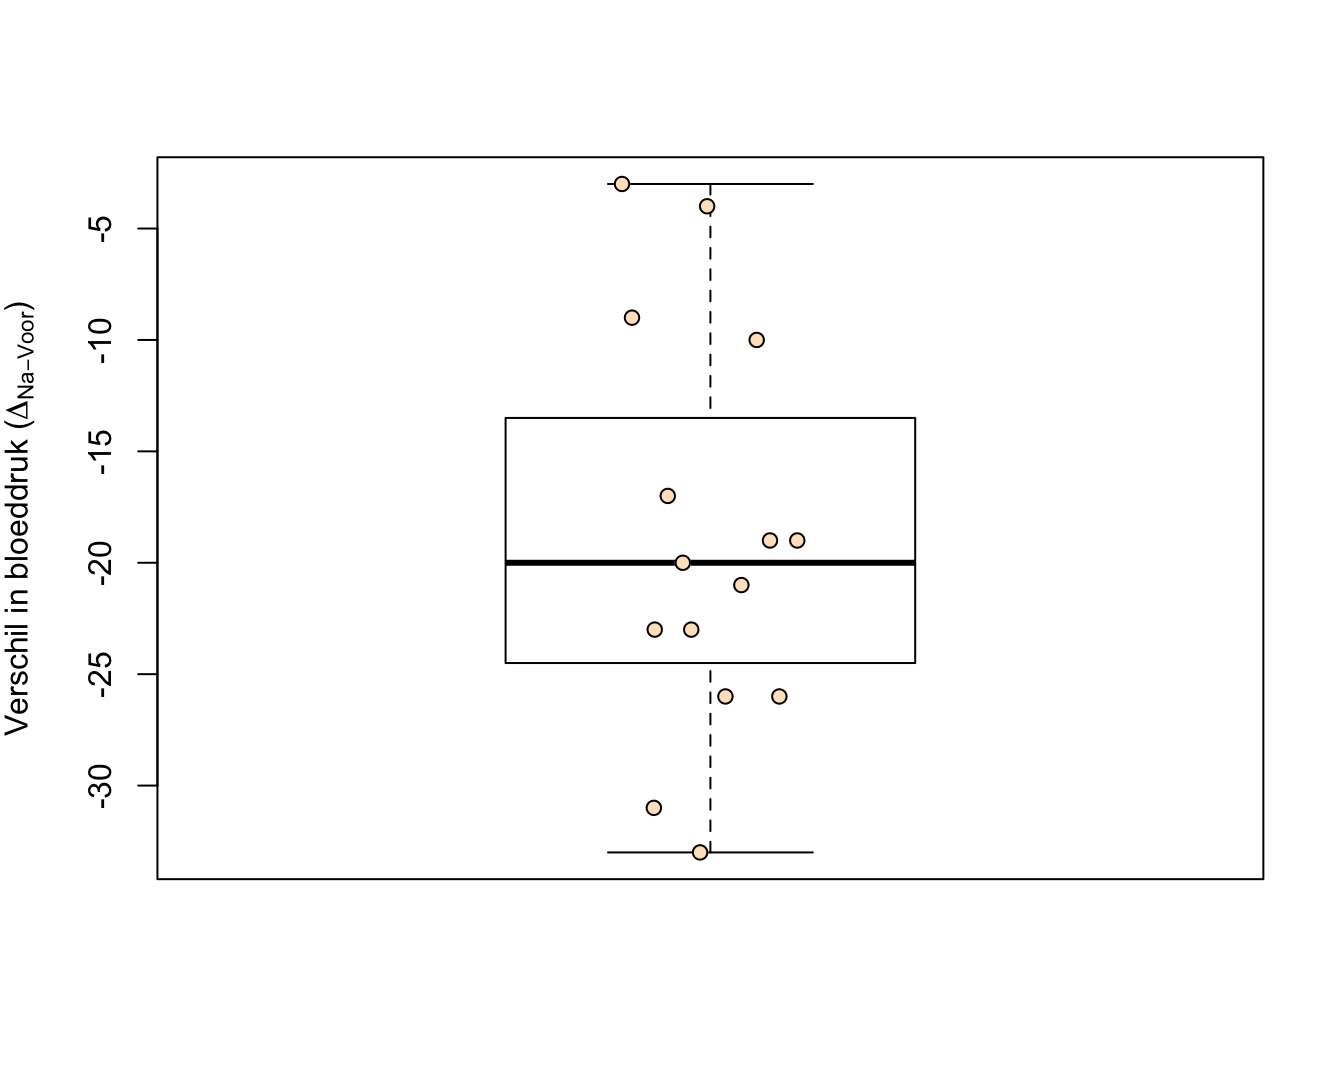
\includegraphics[width=1\linewidth]{Statistiek_2019_2020_files/figure-latex/captoBoxDelta-1} 

}

\caption{Boxplot van het verschil in systolische bloeddruk voor en na het toedienen van captopril.}\label{fig:captoBoxDelta}
\end{figure}

We observeren in Figuur \ref{fig:captoBoxDelta} een bloeddrukdaling voor
elke patiënt in de steekproef wat opnieuw een heel sterke indicatie is
voor een gunstig effect van het toedienen van captopril op de bloeddruk.
De verschillen in systolische bloeddruk zijn een goede maat om het
effect van captopril te bepalen. We kunnen de data als volgt
samenvatten.

\begin{Shaded}
\begin{Highlighting}[]
\KeywordTok{summary}\NormalTok{(delta)}
\end{Highlighting}
\end{Shaded}

\begin{verbatim}
##    Min. 1st Qu.  Median    Mean 3rd Qu.    Max. 
##  -33.00  -24.50  -20.00  -18.93  -13.50   -3.00
\end{verbatim}

\begin{Shaded}
\begin{Highlighting}[]
\KeywordTok{sd}\NormalTok{(delta)}
\end{Highlighting}
\end{Shaded}

\begin{verbatim}
## [1] 9.027471
\end{verbatim}

We observeren gemiddeld een systolische bloeddrukdaling van 18.93 mmHg
en een standaard deviatie van 9.03 mmHg.

\subsection{Schatten}\label{schatten}

Pre-test/post-test design: Het effect van captopril in de steekproef kan
worden bestudeerd door het verschil te bepalen in systolische bloeddruk
na en voor de behandeling (\(X=\Delta_\text{na-voor}\))! Hoe kunnen we
de bloeddrukverschillen modelleren en het effect van het toedienen van
captopril schatten?

\begin{figure}

{\centering 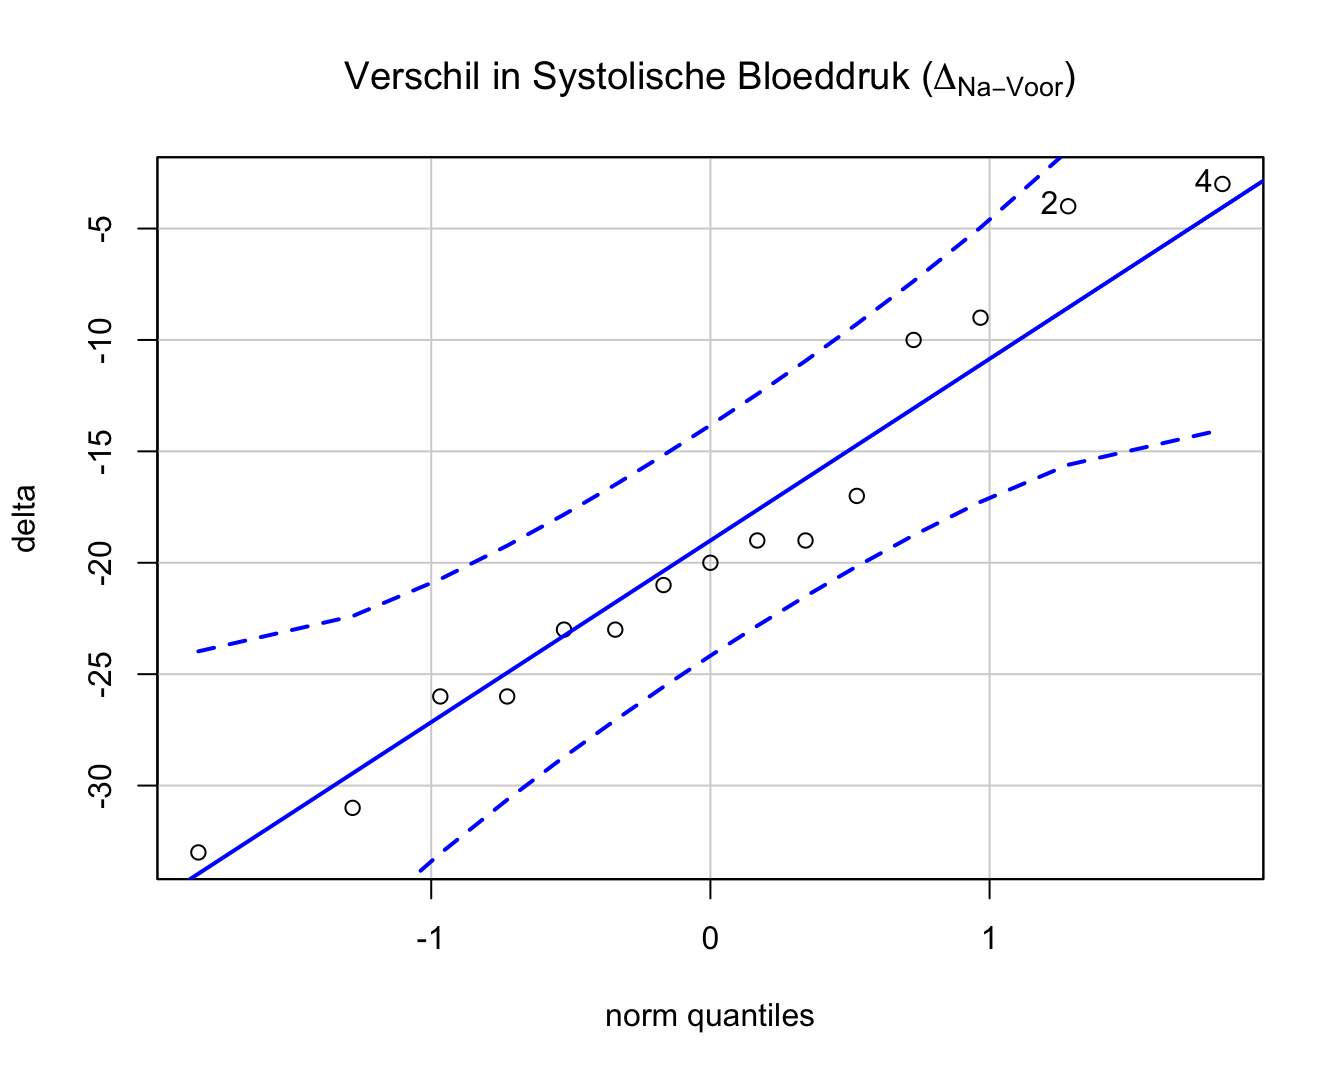
\includegraphics[width=1\linewidth]{Statistiek_2019_2020_files/figure-latex/captoBoxDiffQQ-1} 

}

\caption{QQ-plot voor het verschil in systolische bloeddruk voor en na het toedienen van captopril.}\label{fig:captoBoxDiffQQ}
\end{figure}

\begin{verbatim}
## [1] 4 2
\end{verbatim}

We zien geen grote afwijkingen van Normaliteit in Figuur
\ref{fig:captoBoxDiffQQ}. We kunnen de bloeddrukverschillen dus
modelleren aan de hand van een Normale verdeling en kunnen het effect
van captopril in de populatie beschrijven a.d.h.v. de gemiddelde
bloeddrukverschil \(\mu\). Het bloeddrukverschil \(\mu\) in de populatie
kan worden geschat a.d.h.v. het steekproefgemiddelde \(\bar x\)=-18.93
en de standaard afwijking \(\sigma\) a.d.h.v. de
steekproefstandaarddeviatie \(\text{SD}\)=9.03.

We vragen ons nu af of het effect dat we observeren in de steekproef
groot genoeg is om te kunnen spreken van een effect van captopril in de
populatie. We weten immers dat onze statistiek voor de schatting van het
effect van captopril in de populatie berekend wordt op basis van de
gegevens uit de steekproef en daarom zal variëren van steekproef tot
steekproef. Het is daarom belangrijk om een inzicht te krijgen in hoe
het steekproefgemiddelde zal variëren van steekproef tot steekproef.

\section{Puntschatters: het
steekproefgemiddelde}\label{puntschatters-het-steekproefgemiddelde}

Zij \(X\) een lukrake trekking uit de populatie van de bestudeerde
karakteristiek en onderstel dat haar theoretische verdeling{[}bvb. de
Normale verdeling{]} een gemiddelde \(\mu\) en variatie \(\sigma^2\)
heeft. Onderstel bovendien dat we geïnteresseerd zijn in het gemiddelde
\(\mu\) van die karakteristiek in de studiepopulatie. Dan kunnen we
\(\mu\) schatten op basis van een eenvoudige lukrake steekproef,
\(X_1,...,X_n\), als het (rekenkundig) gemiddelde

\begin{equation*}
\bar X = \frac{X_1+ X_2+ ... + X_n}{n} = \frac{\sum_{i=1}^{n} X_i}{n}
\end{equation*}

van de toevalsveranderlijken \(X_1,X_2, ..., X_n\). Dit wordt het
\emph{steekproefgemiddelde} genoemd. Het is belangrijk om te begrijpen
dat het steekproefgemiddelde opnieuw een toevalsveranderlijke\footnote{Om
  die reden duiden we ze aan met een hoofdletter.} is, d.w.z. dat haar
waarde zal variëren van steekproef tot steekproef. Hoewel er slechts 1
populatie is, zijn er heel wat verschillende steekproeven die men
daaruit kan trekken. Dat heeft tot gevolg dat verschillende onderzoekers
(die verschillende steekproeven uit dezelfde populatie analyseren)
verschillende waarden zullen vinden voor het steekproefgemiddelde. Om
die reden heeft het steekproefgemiddelde zelf een verdeling. Men zou die
theoretisch kunnen bekomen door een oneindig aantal keer een steekproef
van \(n\) experimentele eenheden uit de populatie te trekken, telkens
het steekproefgemiddelde te berekenen en al deze steekproefgemiddelden
vervolgens uit te zetten in een histogram.

We zullen in deze sectie de theoretische verdeling van het
steekproefgemiddelde bestuderen. Dat is belangrijk (a) omdat ze ons
inzicht geeft in welke mate het resultaat van de studie zou variëren
indien men een nieuwe, gelijkaardige studie zou opzetten; en (b) omdat
ze ons leert hoe ver \(\bar X\) van het gezochte populatiegemiddelde
\(\mu\) kan afwijken. Omdat we slechts over 1 steekproef beschikken (en
dus slechts over 1 observatie voor \(\bar X\)), is het niet
evident\footnote{Zo is het met 1 observatie voor \(\bar X\) niet
  mogelijk om een histogram voor \(\bar X\) uit te zetten.} hoe we
inzicht kunnen ontwikkelen in de verdeling van het steekproefgemiddelde.
In het vervolg van deze sectie tonen we hoe dit toch mogelijk is op
basis van de beschikbare steekproef wanneer we bepaalde aannames doen
over de gegevens.

\subsection{Het steekproefgemiddelde is
onvertekend}\label{het-steekproefgemiddelde-is-onvertekend}

In de praktijk hoopt men uiteraard dat de schattingen die men bekomt op
basis van de steekproef vergelijkbaar zijn met de overeenkomstige
populatieparameters die men voor de volledige populatie zou bekomen.\\
Of dat zo is, hangt er in eerste instantie vanaf of de steekproef
representatief is voor de studiepopulatie en bijgevolg of men al dan
niet lukraak individuen uit de populatie gekozen heeft ter observatie
(m.a.w. het hangt af van het design van de studie). Het volgende
voorbeeld illustreert dit.

\BeginKnitrBlock{example}[Ecstasy]
\protect\hypertarget{exm:unnamed-chunk-64}{}{\label{exm:unnamed-chunk-64}
\iffalse (Ecstasy) \fi{} }
\EndKnitrBlock{example} Aan Stanford University werd een survey
uitgevoerd om de prevalentie van ecstasy-gebruik onder de studenten van
deze universiteit te bepalen. Twee assistenten werden op het hoofdplein
van de campus geplaatst en kregen de opdracht om alle studenten te
interviewen die op bepaalde tijdstippen voorbij kwamen. Van de 369
studenten die geïnterviewd werden, rapporteerde 39\% ooit ecstasy
gebruikt te hebben. Dit resultaat wordt uiteraard deels bepaald door het
algemene ecstasy-gebruik onder Stanford-studenten (d.i. door de
verdeling van het ecstasy-gebruik over de populatie van
Stanford-studenten). Maar ook door het feit dat de studenten die
geïnterviewd werden, vermoedelijk een selectieve groep vormen van
studenten die bijvoorbeeld niet in de les aanwezig waren of die in de
buurt van het hoofdplein les kregen en bijgevolg voornamelijk uit 1
bepaalde studierichting afkomstig waren.

\texttt{**Einde\ voorbeeld**}

Omwille hiervan is het design van een studie van primair belang om
lukrake en representatieve steekproeven te garanderen (zie Sectie
\ref{sec:steekproefdesigns}). Zoals u doorheen deze cursus zult
vaststellen, zullen de meeste wetenschappelijke rapporten daarom een
gedetailleerde beschrijving geven van de manier waarop de data bekomen
werden. Dit moet de lezer toelaten om de validiteit van de studie te
beoordelen.

Algemeen zullen we met \(E(X)\), \(\text{Var}(X)\) en
\(\text{Cor}(X,Y)\) respectievelijk het gemiddelde, de variantie en de
correlatie noteren van 2 toevalsveranderlijken \(X\) en \(Y\) in de
populatie. Deze worden respectievelijk de \emph{theoretische
verwachtingswaarde} van \(X\), \emph{theoretische variantie} van \(X\)
en \emph{theoretische correlatie} van \(X\) en \(Y\) genoemd. Men zou ze
bekomen door voor alle individuen in de populatie de karakteristieken
\(X\) en \(Y\) op te meten en vervolgens respectievelijk het rekenkundig
gemiddelde, de variantie en de Pearson correlatie te berekenen. Om die
reden blijven de rekenregels voor gemiddelden en varianties
geldig\footnote{In principe is een meer theoretische, mathematische
  ontwikkeling nodig omdit aan te tonen, maar voor het bestek van deze
  cursus volstaat het om het meer intuïtieve argument aan te nemen.}
voor populatiegemiddelden en -varianties.

In de onderstelling dat we over een eenvoudige lukrake steekproef
beschikken van metingen \(X_1,...,X_n\) voor een karakteristiek \(X\),
volgen \(X_1,...,X_n\) allen dezelfde verdeling. In het bijzonder hebben
ze allen gemiddelde \(\mu\) en variantie \(\sigma^2\); d.i.
\(E(X_1)=...=E(X_n)=\mu\) en
\(\text{Var}(X_1)=...=\text{Var}(X_n)=\sigma^2\). Het feit dat we
subjecten 1 tot \(n\) lukraak uit de populatie getrokken hebben, staat
er m.a.w. garant voor dat verdeling van de karakteristiek in deze
steekproef representatief is voor de theoretische verdeling in de
doelpopulatie. Gebruik makend van de rekenregels voor gemiddelden,
vinden we bijgevolg dat:

\begin{eqnarray*}
E(\bar X) &=& E \left(\frac{X_1+ X_2+ ... + X_n}{n}\right) \\
&= & \frac{E(X_1)+ E(X_2)+ ... + E(X_n)}{n} \\
&=& \frac{\mu + \mu + ... +\mu}{n} \\
&= & \mu
\end{eqnarray*}

Dit geeft aan dat het verwachte steekproefgemiddelde in een eenvoudige
lukrake steekproef gelijk is aan het beoogde populatiegemiddelde
\(\mu\). Men zegt dan dat \(\bar X\) een \emph{onvertekende schatter} is
voor \(\mu\). We kunnen in dat geval verwachten dat de waarde \(\bar x\)
die we schatten voor \(\mu\) op basis van de steekproef, niet
systematisch hoger of lager dan de gezochte waarde \(\mu\) zal zijn. Het
spreekt voor zich dat dit een zeer wenselijke eigenschap is.

\BeginKnitrBlock{definition}[Onvertekende schatter]
\protect\hypertarget{def:unnamed-chunk-65}{}{\label{def:unnamed-chunk-65}
\iffalse (Onvertekende schatter) \fi{} }Een statistiek of schatter \(S\)
voor een parameter \(\theta\) wordt \textbf{onvertekend} genoemd als
haar theoretische verwachtingswaarde gelijk is aan die parameter, d.w.z.
\(E(S)= \theta\).

\textbf{Einde definitie}
\EndKnitrBlock{definition}

\subsection{Imprecisie/standard error}\label{imprecisiestandard-error}

Het feit dat het steekproefgemiddelde (over een groot aantal
vergelijkbare studies) \emph{gemiddeld} gezien niet afwijkt van de
gezochte waarde \(\mu\), impliceert niet dat ze niet rond die waarde
varieert. Om inzicht te krijgen hoe dicht we het steekproefgemiddelde
bij \(\mu\) mogen verwachten, wensen we bijgevolg ook haar variabiliteit
te kennen. Om dit te bepalen, zullen we ervan uitgaan dat de metingen
\(X_1, X_2, ..., X_n\) werden gemaakt bij \(n\) \emph{onafhankelijke}
observationele eenheden. In woorden betekent onafhankelijkheid dat elk
subject een volledig nieuw stukje informatie bijdraagt tot het geheel.
Een voorbeeld van afhankelijkheid tussen studie-objecten komt klassiek
uit de studie van kankerverwekkende stoffen. Bij testen op zwangere
ratten, worden metingen gedaan op hun levende foetussen of boorlingen.
Foetussen van eenzelfde moeder delen dezelfde genetische achtergrond en
zijn daarom waarschijnlijk meer aan elkaar gelijk dan foetussen van
verschillende moeders. Zelfs al zijn de moeders die opgenomen worden in
zo'n studie onafhankelijk van elkaar gekozen, de verschillende kleine
ratjes leveren niet langer onafhankelijke stukjes informatie: via de
gedeelde moeders is een afhankelijkheid ingebouwd. Afhankelijke gegevens
worden ondermeer ook verzameld in pre-test/post-test designs en
cross-over studies. De volgende eigenschap illustreert de noodzaak om
over onafhankelijke gegevens te beschikken, wil men gemakkelijk de
variabiliteit van het steekproefgemiddelde kunnen bepalen.

\textbf{Eigenschap}

Als \(X\) en \(Y\) onafhankelijke toevalsveranderlijken zijn, dan
geldt\footnote{Merk op dat de vierkantswortel van een som niet gelijk is
  aan de som van de vierkantswortels. Bijgevolg is de standaarddeviatie
  van de som van \(X\) en \(Y\) niet de som van de corresponderende
  standaarddeviaties!}:

\begin{equation*}
\text{Var}(X+Y) = \text{Var}(X) + \text{Var}(Y)
\end{equation*}

Algemeen (d.i. voor mogelijks afhankelijke toevalsveranderlijken \(X\)
en \(Y\)) geldt voor constanten \(a\) en \(b\):

\begin{eqnarray*}
\text{Var}(aX+bY) &=& a^2 \text{Var}(X) + b^2 \text{Var}(Y) + 2 ab {%
\text{Cor}}(X,Y)\sqrt{\text{Var}(X)}\sqrt{\text{Var}(Y)}
\end{eqnarray*}

\textbf{Einde Eigenschap}

Een veelgemaakte fout is dat men beweert dat
\(\text{Var}(X-Y)=\text{Var}(X)-\text{Var}(Y)\). Niets is minder waar!
Stel bijvoorbeeld dat de lengte \(X\) van moeders en de lengte \(Y\) van
vaders evenveel variëren zodat \(\text{Var}(X)=\text{Var}(Y)\). Dan
impliceert dat nog niet dat als je het verschil \(X-Y\) neemt tussen de
lengte van een moeder en haar partner, dat dit verschil variantie nul
heeft; d.w.z. dat het niet varieert en bijgevolg voor alle moeder-vader
paren exact dezelfde waarde aanneemt! Bovenstaande formules geven
inderdaad integendeel aan dat:

\begin{equation*}
\text{Var}(X-Y) = \text{Var}(X) + \text{Var}(Y) -2{\text{Cor}}(X,Y)\sqrt{\text{Var}(X)}\sqrt{\text{Var}(Y)}.
\end{equation*}

Gebruik makend van deze rekenregels en steunend op de onafhankelijkheid
van de observaties (waarvan we gebruik maken in de derde overgang, *)
kunnen we nu verder berekenen dat:

\begin{eqnarray*}
\text{Var}(\bar X)&=&\text{Var} \left(\frac{X_1+ X_2+ ... + X_n}{n}\right) \\
&= & \frac{\text{Var} (X_1+ X_2+ ... + X_n)}{n^2} \\
&\overset{*}{=} & \frac{\text{Var}(X_1)+ \text{Var}(X_2)+ ... + \text{Var}(X_n)}{n^2} \\
&=& \frac{\sigma^2 + \sigma^2 + ... \sigma^2}{n^2} \\
&= & \frac{\sigma^2}{n}.
\end{eqnarray*}

Het steekproefgemiddelde heeft dus een spreiding (standaarddeviatie)
rond haar gemiddelde \(\mu\) die \(\sqrt{n}\) keer kleiner is dan de
deviatie op de oorspronkelijke observaties. Vandaar dat we meer over
\(\mu\) kunnen leren door het steekproefgemiddelde \(\bar X\) te
observeren dan door een individuele waarde \(X\) te observeren.

\BeginKnitrBlock{definition}[Standaard error]
\protect\hypertarget{def:unnamed-chunk-66}{}{\label{def:unnamed-chunk-66}
\iffalse (Standaard error) \fi{} }De standaarddeviatie van \(\bar{X}\)
is \(\sigma/\sqrt{n}\) en krijgt in de literatuur de speciale naam
\{standard error\} van het gemiddelde. Algemeen noemt men de
standaarddeviatie van een schatter voor een bepaalde parameter
\(\theta\), de \textbf{standard error} van die schatter. Men noteert dit
als \(SE\).

\textbf{Einde definitie}
\EndKnitrBlock{definition}

\BeginKnitrBlock{example}[Gemiddelde bloeddrukverandering]
\protect\hypertarget{exm:unnamed-chunk-67}{}{\label{exm:unnamed-chunk-67}
\iffalse (Gemiddelde bloeddrukverandering) \fi{} }
\EndKnitrBlock{example} Stel dat we \(n = 15\) systolische
bloeddrukobservaties zullen meten en dat de standaarddeviatie van de
bloeddrukverschillen in de populatie \(\sigma = 9.0\) mmHg bedraagt, dan
is standard error (SE) van de systolische bloeddrukveranderingen
\(\bar X\): \[
SE= \frac{9.0}{\sqrt{15}}=2.32\text{mmHg.}
\]

Meestal is \(\sigma\), en bijgevolg de standard error van het
steekproefgemiddelde, ongekend. Men moet dan de standard error schatten.
Een voor de hand liggende schatter met goede eigenschappen is
\(S/\sqrt{n},\) waarbij \(S^2\) de \emph{steekproefvariantie} van de
reeks observaties \(X_1,...,X_n\) is en \(S\) de \emph{steekproef
standaarddeviatie} wordt genoemd.

Voor het captopril voorbeeld kunnen we de standard error op het
steekproefgemiddelde van de bloeddrukveranderingen schatten in R als

\begin{Shaded}
\begin{Highlighting}[]
\NormalTok{n =}\StringTok{ }\KeywordTok{length}\NormalTok{(delta)}
\NormalTok{se =}\StringTok{ }\KeywordTok{sd}\NormalTok{(delta)}\OperatorTok{/}\KeywordTok{sqrt}\NormalTok{(n)}
\NormalTok{se}
\end{Highlighting}
\end{Shaded}

\begin{verbatim}
## [1] 2.330883
\end{verbatim}

\subsubsection{Standaarddeviatie vs standard
error}\label{standaarddeviatie-vs-standard-error}

Er is vaak nogal wat verwarring over het onderscheid tussen standard
error en standaarddeviatie. De standard error verwijst steeds naar de
spreiding op een geschatte parameter zoals het steekproefgemiddelde.
Omdat een schatting steeds precieser wordt naarmate de steekproef groter
wordt, daalt de standard error met stijgende steekproefgrootte \(n\).
Als de term standaarddeviatie verwijst naar het steekproefgemiddelde
(m.a.w. als men spreekt over de standaarddeviatie van het
steekproefgemiddelde), dan is deze standaarddeviatie identiek gelijk aan
de standard error. Als ze verwijst naar de individuele observaties, dan
niet. Dit kun je ondermeer zien aan het feit dat de individuele
observaties niet minder variabel zijn in grote steekproeven dan in
kleine steekproeven; m.a.w. de standaarddeviatie van de individuele
observaties neemt niet af naarmate de steekproef groter wordt, het is
immers een karakteristiek van de populatie.

De standaarddeviatie op de observaties is een maat voor de variabiliteit
tussen individuen met betrekking tot een bepaalde meetwaarde. De
standaard error van een schatter meet de onzekerheid in die schatter
voor een bepaalde parameter.

Beide statistieken worden ook anders beïnvloed door de
steekproefgrootte. De variabiliteit in de populatie verandert niet.
Buiten het feit dat we de standaarddeviatie meer nauwkeurig kunnen
schatten in een grotere steekproef zal ze dus steeds in dezelfde
grootteorde liggen. Ze heeft als verwachte waarde immers de theoretische
standaarddeviatie \(\sigma\) in de populatie. De standard error van een
schatter wordt echter sterk beïnvloed door de steekproefgrootte: hoe
groter de steekproef hoe nauwkeuriger de schatter voor een bepaalde
parameter en hoe kleiner zijn standard error!

\subsubsection{Geclusterde metingen}\label{geclusterde-metingen}

De data in studies zijn niet altijd onafhankelijk. Dat heeft zijn
consequenties voor het schatten van de standaard errors. Beschouw een
studiedesign waarbij voor \(n\) planten, tijdens een bepaalde fase in de
groei, de expressie van een bepaald gen 2 maal wordt gemeten om
meetfouten te drukken. Men is geïnteresseerd in de gemiddelde
genexpressie. Als we met \(Y_{i1}\) en \(Y_{i2}\) de eerste en tweede
meting, respectievelijk, voorstellen voor plant \(i=1,...,n\), dan
kunnen we dit schatten als

\begin{equation*}
\bar Y = \sum_{i=1}^n \frac{Y_{i1}+Y_{i2}}{2n}
\end{equation*}

In de onderstelling dat de \(n\) planten onafhankelijk van elkaar
gekozen werden en de eerste en tweede metingen even variabel zijn
(d.w.z. \(\text{Var}(Y_{i1})=\text{Var}(Y_{i2})=\sigma^2\)), bedraagt de
variantie op dit steekproefgemiddelde

\begin{eqnarray*}
\text{Var}(\bar Y)&=&\sum_{i=1}^n \frac{\text{Var}(Y_{i1}+Y_{i2})}{4n^2} \\
&=&\sum_{i=1}^n \frac{\sigma^2+\sigma^2+2\text{Cor}(Y_{i1},Y_{i2})\sigma^2}{%
4n^2} \\
&=&\frac{\sigma^2}{2n}\{1+\text{Cor}(Y_{1},Y_{2})\}
\end{eqnarray*}

Vermits verschillende metingen afkomstig van eenzelfde plant doorgaans
positief met elkaar gecorreleerd zijn, is de standard error op
\(\bar Y\) dus groter dan wanneer de \(2n\) metingen van \(2n\)
verschillende, onafhankelijke planten afkomstig zouden zijn. Dat is
omdat, gegeven de eerste meting \(Y_{i1}\), de tweede meting \(Y_{i2}\)
geen volledig nieuwe informatie toevoegt en er bijgevolg minder
informatie beschikbaar is om het gemiddelde te schatten dan wanneer alle
gegevens van verschillende planten afkomstig waren. In het bijzonder,
wanneer \(\text{Cor}(Y_{1},Y_{2})=1\), dan levert de tweede meting geen
nieuwe informatie en bekomt men eenzelfde nauwkeurigheid als wanneer men
slechts 1 meting per plant had bekomen. Wanneer
\(\text{Cor}(Y_{1},Y_{2})=0\), dan levert de tweede meting volledig
nieuwe informatie en bekomt men eenzelfde nauwkeurigheid als wanneer men
1 meting had bekomen voor \(2n\) i.p.v. \(n\) verschillende planten.
Vermits
\[\frac{\sigma^2}{2n}\{1+\text{Cor}(Y_{1},Y_{2})\}\geq \frac{\sigma^2}{2n}\]

\emph{Wanneer de correlatie tussen herhaalde genexpressie metingen
positief is (hetgeen we verwachten), zal men in de praktijk meer
preciese resultaten bekomen door 1 meting te bepalen voor \(2n\)
verschillende planten dan door 2 metingen te bepalen voor \(n\)
verschillende planten.}

De metingen in de captopril voorbeeld zijn eveneens geclusterd. We
hebben immers twee systolische bloeddrukmetingen per patiënt. 1 meting
voor en 1 meting na het toedienen van captopril. We beogen om de
gemiddelde bloeddrukverandering \(\mu\) te schatten a.d.h.v. de gegevens
\[(Y_{i1} , Y_{i2}),\] voor subjecten \(i = 1, ..., n\). En we bekomen
de volgende schatting: \[\bar X = \sum_{i=1}^n \frac{Y_{i2}-Y_{i1}}{n}\]

Uit de rekenregels voor de variantie weten we dat

\begin{eqnarray*}
\text{Var}\left[\bar X\right]&=&\sum_{i=1}^n \frac{\text{Var}\left[Y_{i1}-Y_{i2}\right]}{n^2}\\
&=&\sum_{i=1}^n \frac{\sigma^2_1+\sigma^2_2-2\text{Cor}\left[Y_{i1},Y_{i2}\right]\sigma_1\sigma_2}{n^2}\\
&=&\frac{\sigma^2_1+\sigma^2_2-2\text{Cor}\left[Y_{i1},Y_{i2}\right]\sigma_1\sigma_2}{n},\\
\end{eqnarray*}

In R kunnen we dit als volgt berekenen:

\begin{Shaded}
\begin{Highlighting}[]
\CommentTok{# functie var op een matrix berekent varianties}
\CommentTok{# sigma_1^2, sigma_2^2 covariantie sigma_\{12\}}
\NormalTok{vars =}\StringTok{ }\KeywordTok{var}\NormalTok{(captopril[, }\KeywordTok{c}\NormalTok{(}\StringTok{"SBPb"}\NormalTok{, }\StringTok{"SBPa"}\NormalTok{)])}
\NormalTok{vars}
\end{Highlighting}
\end{Shaded}

\begin{verbatim}
##          SBPb     SBPa
## SBPb 422.9238 370.7857
## SBPa 370.7857 400.1429
\end{verbatim}

\begin{Shaded}
\begin{Highlighting}[]
\KeywordTok{cor}\NormalTok{(captopril}\OperatorTok{$}\NormalTok{SBPa, captopril}\OperatorTok{$}\NormalTok{SBPb)}
\end{Highlighting}
\end{Shaded}

\begin{verbatim}
## [1] 0.9013312
\end{verbatim}

\begin{Shaded}
\begin{Highlighting}[]
\NormalTok{varXbarDelta =}\StringTok{ }\NormalTok{(vars[}\DecValTok{1}\NormalTok{, }\DecValTok{1}\NormalTok{] }\OperatorTok{+}\StringTok{ }\NormalTok{vars[}\DecValTok{2}\NormalTok{, }\DecValTok{2}\NormalTok{] }\OperatorTok{-}\StringTok{ }\DecValTok{2} \OperatorTok{*}\StringTok{ }\NormalTok{vars[}\DecValTok{1}\NormalTok{, }
    \DecValTok{2}\NormalTok{])}\OperatorTok{/}\DecValTok{15}
\KeywordTok{sqrt}\NormalTok{(varXbarDelta)}
\end{Highlighting}
\end{Shaded}

\begin{verbatim}
## [1] 2.330883
\end{verbatim}

We zien dat de metingen heel sterk gecorreleerd zijn, waardoor de
variantie op het verschil veel lager zal liggen dan op de originele
metingen.

Gezien we voor elke patiënt twee metingen hebben bestaat een
alternatieve methode om de standard error te bepalen erin om alle
gecorreleerde metingen tot 1 meting te reduceren. Merk op dat we dit
enkel kunnen doen voor gepaarde metingen. Alle resulterende metingen
zijn dan onafhankelijk. Concreet kunnen we voor elke patiënt \(i\) in de
steekproef het bloeddrukverschil berekenen: \[X_{i}=Y_{ai}-Y_{bi}\] en
vervolgens standard error op \(\bar X\). In het captopril voorbeeld
wordt de schatting

\begin{Shaded}
\begin{Highlighting}[]
\KeywordTok{sd}\NormalTok{(delta)}\OperatorTok{/}\KeywordTok{sqrt}\NormalTok{(}\DecValTok{15}\NormalTok{)}
\end{Highlighting}
\end{Shaded}

\begin{verbatim}
## [1] 2.330883
\end{verbatim}

We zien dat we exact dezelfde schatting voor de standard error bekomen.
Verder zien we ook dat het design een groot voordeel heeft: Aangezien de
bloeddrukmetingen voor en na het toedienen van captopril sterk positief
gecorreleerd zijn is de variantie van het verschil veel lager dan deze
op de originele bloeddrukmetingen. Iedere patiënt in de studie dient
immers als zijn eigen controle en op die manier kunnen we de
variabiliteit in de bloeddrukmetingen tussen patiënten uit de analyse
verwijderen!

\subsubsection{Normaal verdeelde
gegevens}\label{normaal-verdeelde-gegevens}

Als de gegevens Normaal verdeeld zijn, dan zijn er meerdere onvertekende
schatters voor het populatiegemiddelde \(\mu\), bvb. het
steekproefgemiddelde en de mediaan. Men kan echter aantonen dat in dat
geval het steekproefgemiddelde \(\bar{X}\) de onvertekende schatter is
voor \(\mu\) met de kleinste standard error. Dat betekent dat ze
gemiddeld minder afwijkt van de echte parameterwaarde dan de mediaan,
die veel meer varieert van steekproef tot steekproef. Het
steekproefgemiddelde is bijgevolg een schatter die accuraat is (want
onvertekend) en meest precies (kleinste standaarddeviatie).

\subsection{Verdeling van het
steekproefgemiddelde}\label{subsec:verdelingXbar}

Om ondermeer goed de betekenis van de standard error te kunnen vatten,
moeten we van \(\bar X\) niet alleen het gemiddelde en de
standaarddeviatie, maar ook de exacte verdeling kennen. De standard
error is immers een standaardeviatie (bvb. van het
steekproefgemiddelde), waarvan de betekenis het meest duidelijk is
wanneer de metingen (in dit geval, het steekproefgemiddelde) Normaal
verdeeld zijn. In het bijzonder geval dat de individuele observaties
\(X_i\) een Normale verdeling hebben met gemiddelde \(\mu\) en variantie
\(\sigma^2\), kan men aantonen dat ook \(\bar X\) Normaal verdeeld is
met gemiddelde \(\mu\) en variantie \(\sigma^2/n.\) Dit fenomeen wordt
geïllustreerd in Figuur \ref{fig:meansim}. De linkse figuur illustreert
een lukrake trekking of steekproef van observaties uit een Normale
verdeling. Als men dit blijft herhalen en voor alle bekomen steekproeven
het steekproefgemiddelde berekent en en vervolgens deze gemiddeldes
uitzet in een histogram, dan krijgt men het histogram uit rechtse
figuur. De steekproefgemiddeldes in deze figuur lijken inderdaad een
Normale verdeling te volgen.

\begin{figure}

{\centering 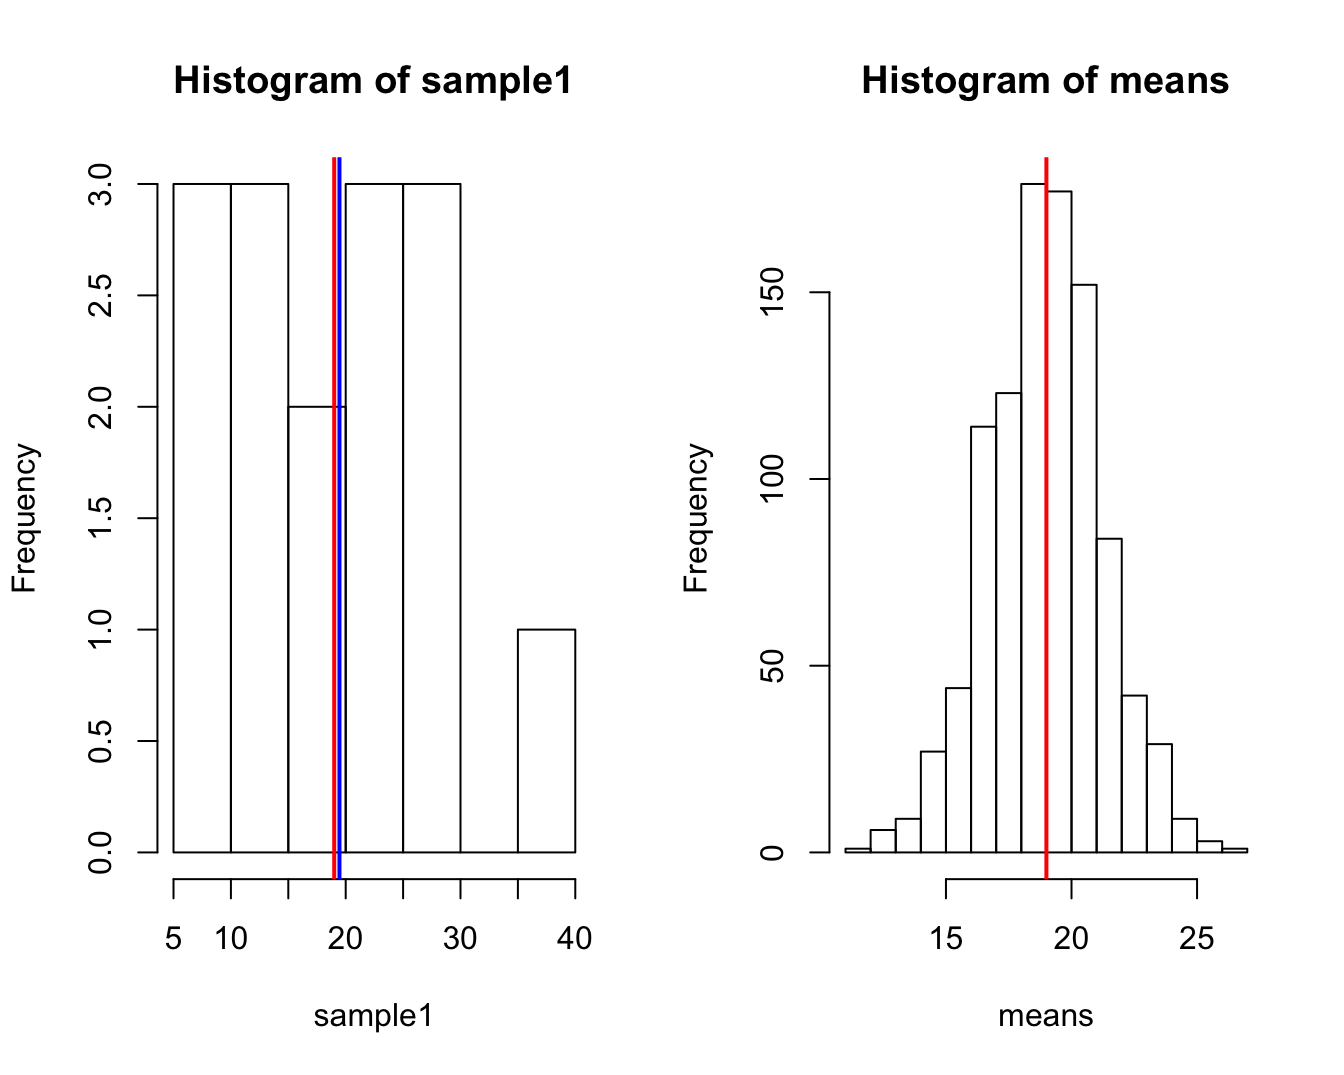
\includegraphics[width=1\linewidth]{Statistiek_2019_2020_files/figure-latex/meansim-1} 

}

\caption{Simulaties van steekproeven met n=15 observaties uit een normale verdeling met gemiddelde systolische bloeddrukdaling 19 mmHg en standaard deviate van 9 mmHg. (links één steekproef, rechts een histogram van steekproefgemiddelden voor 1000 steekproeven. Het gemiddelde in de populatie is weergegeven d.m.v. rode lijn).}\label{fig:meansim}
\end{figure}

In het captopril voorbeeld zagen we dat de systolische
bloeddrukverandering approximatief normaal verdeeld is. De standard
error op de bloeddrukverandering bedroeg 2.32 mm Hg. Dus op 100 studies
met n = 15 subjecten, verwachten we dat de geschatte gemiddelde
systolische bloeddrukafwijking (\(\bar X\)) op minder dan 2 × 2.32 =
4.64mm Hg van het werkelijke populatiegemiddelde (\(\mu\)) ligt in 95
studies.

In het algemeen, wanneer de individuele observaties \(X_i\) geen Normale
verdeling hebben, is \(\bar X\) \textit{bij benadering} toch nog Normaal
verdeeld zodra het aantal observaties groot genoeg is. Hoe groot de
steekproef hiervoor moet zijn, hangt hierbij af van hoe scheef de
verdeling van de oorspronkelijke observaties is. Dat is het gevolg van
de volgende fundamentele en veel toegepaste wiskundestelling.

\textbf{De Centrale Limietstelling (CLT)}

Stel dat \(X_1, X_2, \dots, X_n, \; n\) onafhankelijke lukrake
trekkingen van de toevalsveranderlijke \(X\) voorstellen, met allen
dezelfde theoretische verdeling. Laat \(X\) gemiddelde \(\mu\) en
variantie \(\sigma^2\) hebben maar verder een ongespecifieerde
verdeling, dan wordt de verdeling van het steekproefgemiddelde
\(\bar{X}_n = {\sum_{i=1}^{n} X_i}/{n}\) naarmate \(n\) groter wordt
steeds beter benaderd door de Normale verdeling met gemiddelde \(\mu\)
en variantie \(\sigma^2/n.\)

\textbf{Einde Stelling}

Deze belangrijke eigenschap zal ons toelaten om de meeste technieken die
in deze cursus aan bod komen toe te passen op een zeer uitgebreid
spectrum van experimenten.

We illustreren deze stelling in Figuur \ref{fig:CLT}. We simuleren data
uit een experiment waarbij we een munt opwerpen. De data zijn dan
Bernouilli verdeeld en kunnen de waarde \(X=0\) (munt) of \(X=1\) (kop)
aannemen met een kans van 50\% en zijn duidelijk niet-Normaal verdeeld.
We simuleren steekproeven met een steekproefgrootte van 10 observaties
en 100 observaties en onderzoeken de verdeling van het
steekproefgemiddelde voor elke steekproefgrootte. We zien duidelijk dat
CLT niet van toepassing is bij een steekproefgrootte van 10. Voor
steekproeven met 100 observaties zien we dat de verdeling van het
steekproefgemiddelde al beter benaderd kan worden door een Normale
verdeling.

\begin{figure}

{\centering 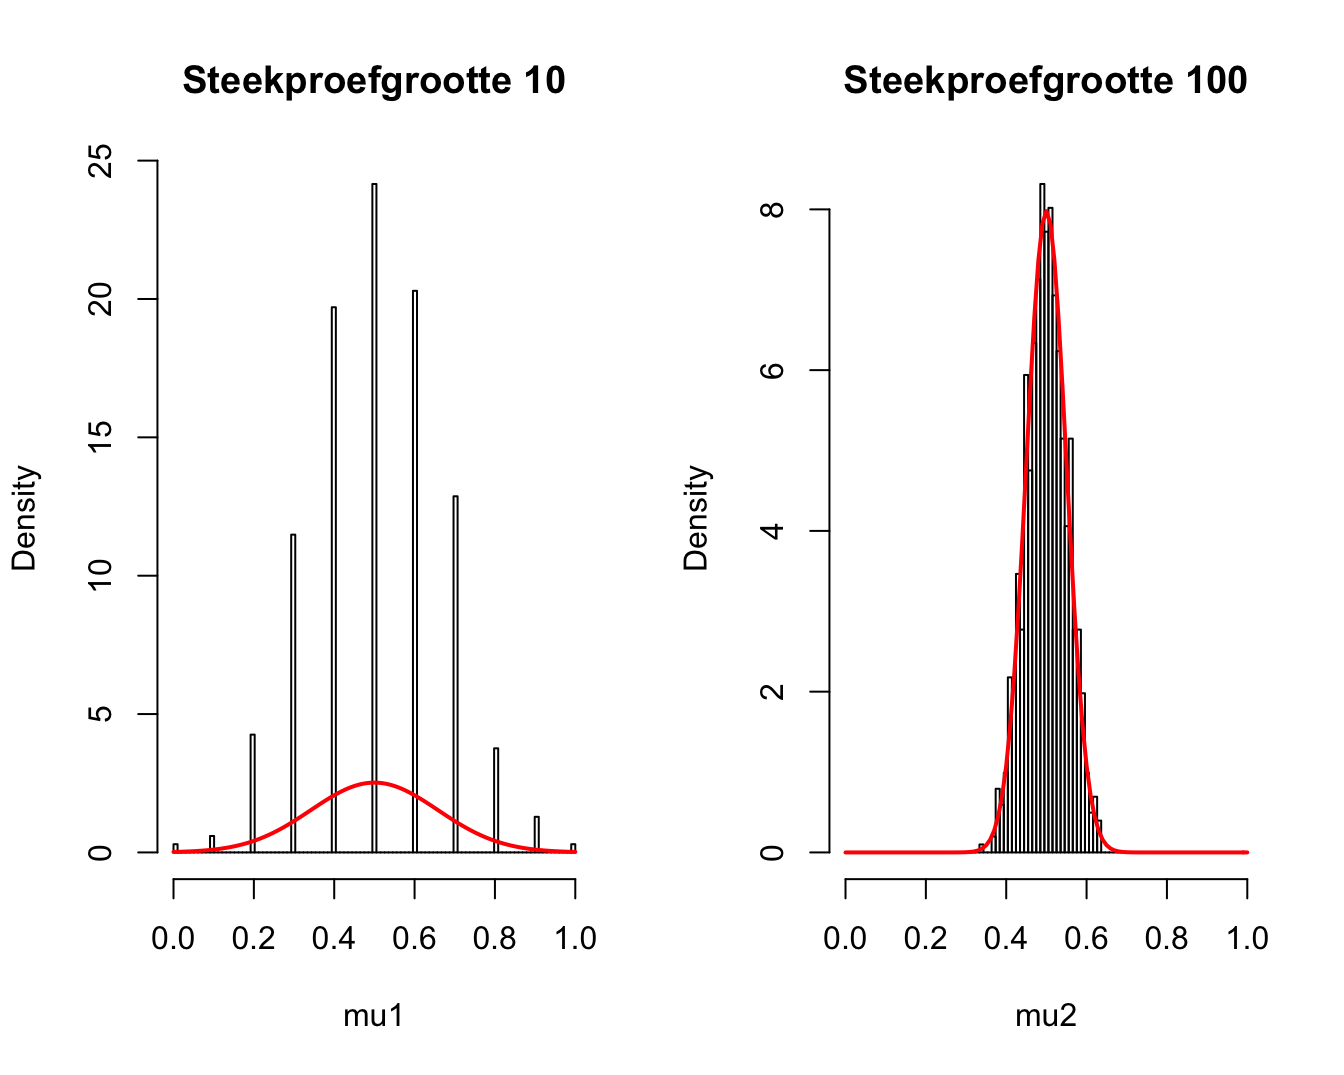
\includegraphics[width=1\linewidth]{Statistiek_2019_2020_files/figure-latex/CLT-1} 

}

\caption{Illustratie van de Centrale Limietstelling d.m.v. Bernouilli verdeelde gegevens (opwerpen van een muntstuk) Steekproefgroottes (n=10, links, en n=100, rechts). Densiteit van de normale verdeling worden weergegeven in rood. We zien duidelijk dat CLT niet van toepassing is bij een steekproefgrootte van 10. Voor steekproeven met 100 observaties zien we dat de verdeling van het steekproefgemiddelde al beter benaderd kan worden door een Normale verdeling.}\label{fig:CLT}
\end{figure}

\section{Intervalschatters}\label{intervalschatters}

In de vorige sectie hebben we vastgesteld dat het steekproefgemiddelde
van steekproef tot steekproef varieert rond het populatiegemiddelde dat
we willen schatten. Om die reden wensen we in deze sectie een interval
rond het steekproefgemiddelde te bepalen waarbinnen we het
populatiegemiddelde met gegeven kans (bvb. 95\% kans) kunnen verwachten.
In Sectie \ref{subsec:bigek} zullen we dit uitwerken voor het geval waar
de populatievariantie \(\sigma^2\) op de metingen gekend is. Deze
onderstelling is meestal onredelijk\footnote{Denk zelf maar eens na of
  je gevallen kunt bedenken waar je al op voorhand, zonder ook maar
  observaties te zien, de variantie op een bepaalde karakteristiek
  kent\ldots{}}, maar wordt hier gemaakt om redenen van eenvoud. In
Sectie \ref{sec:tBI} zullen we van deze onderstelling afstappen.

\subsection{Gekende variantie op de metingen}\label{subsec:bigek}

Wanneer de individuele observaties \(X\) Normaal verdeeld zijn met
gemiddelde \(\mu\) en gekende variantie \(\sigma^2\), noteren we dat als
volgt: \(X\sim N(\mu,\sigma^2)\). Uit vorige sectie volgt dan dat het
steekproefgemiddelde \(\bar{X}\) eveneens Normaal verdeeld is volgens
\(N(\mu,\sigma^2/n)\). Een 95\% referentie-interval voor het
steekproefgemiddelde ziet er bijgevolg uit als

\begin{equation*}
\left[\mu - 1.96 \frac{\sigma}{\sqrt{n}},\mu + 1.96 \frac{\sigma}{\sqrt{n}}%
\right]
\end{equation*}

Het bevat met 95\% kans het steekproefgemiddelde van een lukrake
steekproef. Dit interval kunnen we niet expliciet berekenen op basis van
de geobserveerde gegevens, omdat \(\mu\) ongekend is (we gaan er hier
voorlopig van uit dat \(\sigma\) wel gekend is). Het kan wel geschat
worden als

\begin{equation*}
\left[\bar X - 1.96 \frac{\sigma}{\sqrt{n}},\bar X + 1.96 \frac{\sigma}{\sqrt{n}}\right]
\end{equation*}

Hoewel dit laatste interval nog steeds kan geïnterpreteerd worden als
een referentie-interval voor het steekproefgemiddelde, kunnen we er een
veel nuttigere interpretatie aan geven. Immers, de ongelijkheid
\(\mu - 1.96 \
\sigma/\sqrt{n} < \bar{X}\) kan equivalent worden herschreven als
\(\mu < \bar{X} + 1.96 \ \sigma/\sqrt{n}\). Hieruit volgt:

\begin{eqnarray*}
95\% &=& P( \mu - 1.96 \ \sigma/\sqrt{n} < \bar{X} < \mu + 1.96 \ \sigma/\sqrt{n} ) \\
&=&P( \bar{X} - 1.96 \ \sigma/\sqrt{n} < \mu < \bar{X} + 1.96 \ \sigma/\sqrt{n} )
\end{eqnarray*}

Dit leidt tot volgende definitie.

\BeginKnitrBlock{definition}[95$\%$ betrouwbaarheidsinterval voor populatiegemiddelde]
\protect\hypertarget{def:unnamed-chunk-71}{}{\label{def:unnamed-chunk-71}
\iffalse (95\(\%\) betrouwbaarheidsinterval voor populatiegemiddelde)
\fi{} }Het interval

\begin{equation}  
[\bar{X} - 1.96 \ \sigma/\sqrt{n} , \bar{X} + 1.96 \ \sigma/\sqrt{n} ], \label{eq:bi}
\end{equation}

bevat met 95\% kans het populatiegemiddelde \(\mu\). Het wordt een
\textbf{95\% betrouwbaarheidsinterval} (in het Engels: \emph{95\%
confidence interval}) voor het populatiegemiddelde \(\mu\) genoemd. De
kans dat het de populatieparameter \(\mu\) bevat, d.i. 95\%, wordt het
\emph{betrouwbaarheidsniveau} genoemd.

\textbf{Einde definitie}
\EndKnitrBlock{definition}

Een 95\% betrouwbaarheidsinterval bepaalt met andere woorden een reeks
waarden waarbinnen de gezochte populatieparameter \emph{waarschijnlijk}
(namelijk met 95\% kans) valt.

Stel dat we in een steekproef een bloeddrukdaling van -18.93mmHg
observeren en dat we weten dat de standaarddeviatie van de
bloeddrukmetingen 9mmHg bedraagt. Dan vinden we een
betrouwbaarheidsinterval voor de gemiddelde bloeddrukdaling van
\(\left[-18.93-1.96\times 9/\sqrt{15},-18.9+1.95\times 9/\sqrt{15}\right]=\){[}-23.48,-14.38{]}mmHg.

De reden waarom over ``95\% kans'' gesproken wordt, is omdat de
eindpunten van het 95\% betrouwbaarheidsinterval toevalsveranderlijken
zijn die variëren van steekproef tot steekproef. Met andere woorden,
verschillende steekproeven leveren telkens andere
betrouwbaarheidsintervallen op, vermits die intervallen berekend zijn op
basis van de gegevens in de steekproef. Men noemt het om die reden
\emph{stochastische intervallen}. Voor 95\% van alle steekproeven zal
het berekende 95\% betrouwbaarheidsinterval de gezochte waarde van de
populatieparameter bevatten, en voor de overige 5\% niet. Dat wordt
geïllustreerd a.d.h.v. een simulatiestudie in Sectie
\ref{subsec:interpretBI} (nadat we de intervallen hebben uitgebreid voor
de meer realistische setting waarbij de variantie in de populatie
ongekend is).

Uiteraard kunnen de onderzoekers o.b.v. een gegeven
betrouwbaarheidsinterval niet besluiten of het de gezochte
parameterwaarde bevat of niet, vermits ze precies op zoek zijn naar die
onbekende waarde. Maar ze gebruiken een procedure die in 95\% van de
gevallen werkt; m.a.w. die in 95\% van de gevallen de gezochte waarde
bevat. Of nog, als men dagelijks gegevens zou verzamelen en telkens een
95\% betrouwbaarheidsinterval zou berekenen voor een nieuwe parameter
\(\theta\) (bvb. een odds ratio), dan zou men op lange termijn in 95\%
van de gevallen de gezochte waarde omvat hebben.

Tot nog toe zijn we ervan uitgegaan dat de individuele observaties
Normaal verdeeld zijn en dat hun variantie gekend is (want als de
variantie \(\sigma^2\) niet gekend is, kan men de grenzen van het
interval niet berekenen). Wegens de Centrale Limietstelling bevat
Vergelijking \eqref{eq:bi} het gemiddelde \(\mu\) bij benadering met 95\%
kans wanneer de steekproef groot is en de variantie van de individuele
observaties gekend, maar hun verdeling ongekend is.

Wanneer bovendien de variantie ongekend is, kan me ze schatten door
gebruik te maken van de steekproefvariantie \(S^2\) van de reeks
observaties \(X_1,...,X_n\). Men kan aantonen dat het interval
\([\bar{X} - 1.96 \ s/\sqrt{n} , \bar{X} + 1.96 \ s/\sqrt{n} ]\) dan het
populatiegemiddelde met bij benadering 95\% kans bevat, op voorwaarde
dat de steekproef groot is. In de volgende sectie gaan we na hoe een
betrouwbaarheidsinterval voor het populatiegemiddelde geconstrueerd kan
worden wanneer de variantie ongekend is en de steekproef relatief klein.

Om een betrouwbaarheidsinterval met een ander betrouwbaarheidsniveau,
\((1- \alpha)100\%\) te construeren, vervangt men 1.96 door het
relevante kwantiel \(z_{\alpha/2}.\)

De breedte van een \(100\%(1-\alpha)\) betrouwbaarheidsinterval voor een
populatiegemiddelde \(\mu\) is \(2 z_{\alpha/2} \ \sigma/\sqrt{n}\). Ze
wordt dus bepaald door 3 factoren: de standaarddeviatie op de
individuele observaties, \(\sigma\), de grootte van de steekproef,
\(n\), en het betrouwbaarheidsniveau, \(1-\alpha\):

\begin{itemize}
\item
  \(n\): naarmate de steekproefgrootte toeneemt, krimpt het
  betrouwbaarheidsinterval. In grote steekproeven beschikken we immers
  over veel informatie en kunnen we de gezochte populatieparameter
  bijgevolg relatief nauwkeurig afschatten.
\item
  \(\sigma\): naarmate de standaarddeviatie van de oorspronkelijke
  observaties toeneemt, neemt de lengte van het betrouwbaarheidsinterval
  toe. Indien er immers veel ruis op de gegevens zit, dan is het
  moeilijker om populatieparameters of -kenmerken te identificeren.
\item
  \(1-\alpha\): naarmate het betrouwbaarheidsniveau toeneemt, wordt het
  betrouwbaarheidsinterval breder. Indien we immers eisen dat het
  interval met 99.9\% kans de populatiewaarde bevat i.p.v. met 80\%
  kans, dan zullen we duidelijk een breder interval nodig hebben.
\end{itemize}

Betrouwbaarheidsintervallen worden niet enkel gebruikt voor het
populatiegemiddelde, maar kunnen in principe voor om het even welke
populatieparameter worden gedefinieerd. Zo kunnen ze bijvoorbeeld
gedefinieerd worden voor een verschil tussen 2 gemiddelden, voor een
odds ratio, voor een variantie, \ldots{} De manier om die intervallen te
berekenen is vaak complex en sterk afhankelijk van de gebruikte schatter
voor de populatieparameter. Er wordt daarom niet van u verwacht dat u
voor alle populatieparameters die we in deze cursus ontmoeten, een
betrouwbaarheidsinterval kunt berekenen, maar wel dat u het kunt
interpreteren.

\BeginKnitrBlock{definition}[Betrouwbaarheidsinterval]
\protect\hypertarget{def:unnamed-chunk-72}{}{\label{def:unnamed-chunk-72}
\iffalse (Betrouwbaarheidsinterval) \fi{} }Een
\textbf{\((1-\alpha)100\)\% betrouwbaarheidsinterval} voor een
populatieparameter \(\theta\) is een geschat (en bijgevolg stochastisch)
interval dat met \((1-\alpha)100\)\% kans de echte waarde van die
populatieparameter \(\theta\) bevat.

\textbf{Einde Definitie}
\EndKnitrBlock{definition}

\subsection{Ongekende variantie op de metingen}\label{sec:tBI}

Tot nog toe werd verondersteld dat de populatievariantie \(\sigma^2\)
gekend is bij het berekenen van een betrouwbaarheidsinterval voor
\(\mu\). Betrouwbaarheidsintervallen voor \(\mu\) werden dan opgebouwd
door op te merken dat de gestandaardiseerde waarde
\((\bar{X} - \mu)/(\sigma/\sqrt{n})\) standaardnormaal verdeeld is en
bijgevolg

\begin{equation*}
\left[\mu - 1.96 \frac{\sigma}{\sqrt{n}},\mu + 1.96 \frac{\sigma}{\sqrt{n}}%
\right]
\end{equation*}

een 95\% referentie-interval voor het steekproefgemiddelde voorstelt.

In de praktijk komt het quasi nooit voor dat men de populatievariantie
\(\sigma^2\) exact kent. In de praktijk wordt deze geschat als \(S^2\)
op basis van de voorhanden zijnde steekproef. Als gevolg hiervan zullen
de betrouwbaarheidsintervallen uit voorgaande sectie doorgaans iets te
smal zijn (omdat ze er geen rekening mee houden dat ook de variantie
werd geschat) en is het noodzakelijk om bij de berekening
\((\bar{X} - \mu)/(S/\sqrt{n})\) te gebruiken als gestandaardiseerde
waarde i.p.v. \((\bar{X} - \mu)/(\sigma/\sqrt{n})\). Wanneer de
steekproef voldoende groot is, ligt de vierkantswortel van variantie
\(S^2\) voldoende dicht bij \(\sigma\) zodat
\({(\bar{X} - \mu)}/{(S/\sqrt{n}) }\) bij benadering een
standaardnormale verdeling volgt en, bijgevolg,

\begin{equation*}
\left[\bar{X} - z_{\alpha/2} \ \frac{S}{\sqrt{n}} , \bar{X} + z_{\alpha/2} \ 
\frac{S}{\sqrt{n}}\right]
\end{equation*}

een benaderd \((1- \alpha)100\%\) betrouwbaarheidsinterval is voor
\(\mu\). Voor kleine steekproeven is dit niet langer het geval. Daardoor
introduceert men een extra onnauwkeurigheid in de gestandaardiseerde
waarde \({(\bar{X} - \mu)}/{(S/\sqrt{n})}\). Deze is nog wel gecentreerd
rond nul en symmetrisch, maar niet langer Normaal verdeeld. De echte
verdeling voor eindige steekproefgrootte \(n\) heeft zwaardere staarten
dan de Normale. Hoeveel zwaarder de staarten zijn, hangt van de
steekproefgrootte \(n\) af. Als \(n\) oneindig groot wordt, komt \(S\)
zodanig dicht bij \(\sigma\) te liggen dat de extra onnauwkeurigheid in
de gestandaardiseerde waarde verwaarloosbaar is en bijgevolg ook het
verschil met de Normale verdeling. Maar voor relatief kleine
steekproeven hangt de verdeling van \({(\bar{X} - \mu)}/({S/\sqrt{n}})\)
af van de grootte \(n\) van de steekproef. Ze krijgt de naam (Student)
\(t\)-verdeling met \(n-1\) vrijheidsgraden (in het Engels:
\emph{degrees of freedom}). Deze verdeling wordt voor een aantal
verschillende vrijheidsgraden geïllustreerd in Figuur \ref{fig:tdist}.
De t-verdelingen in de figuur hebben duidelijk bredere staarten dan de
normaalverdeling, waardoor ze ook een grotere percentielwaarden hebben
voor een vooropgesteld betrouwbaarheidsniveau. Dat zal leiden tot
bredere intervallen, wat logisch is aangezien we de extra onzekerheid
inbouwen die gerelateerd is aan het schatten van de standaarddeviatie.

\BeginKnitrBlock{definition}[t-verdeling]
\protect\hypertarget{def:unnamed-chunk-73}{}{\label{def:unnamed-chunk-73}
\iffalse (t-verdeling) \fi{} }Als \(X_1, X_2, ..., X_n\) een steekproef
vormen uit de Normale verdeling \(N(\mu, \sigma^2)\), dan is
\((\bar{X} - \mu)/(S/\sqrt{n})\) verdeeld als een \(t\)-verdeling met
\(n-1\) vrijheidsgraden.

**Einde Definitie
\EndKnitrBlock{definition}

\begin{Shaded}
\begin{Highlighting}[]
\NormalTok{grid =}\StringTok{ }\KeywordTok{seq}\NormalTok{(}\OperatorTok{-}\DecValTok{5}\NormalTok{, }\DecValTok{5}\NormalTok{, }\FloatTok{0.1}\NormalTok{)}
\KeywordTok{plot}\NormalTok{(grid, }\KeywordTok{dnorm}\NormalTok{(grid), }\DataTypeTok{ylab =} \StringTok{"densiteit"}\NormalTok{, }\DataTypeTok{xlab =} \StringTok{"X"}\NormalTok{, }
    \DataTypeTok{type =} \StringTok{"l"}\NormalTok{, }\DataTypeTok{lwd =} \DecValTok{2}\NormalTok{)}
\NormalTok{dfs =}\StringTok{ }\KeywordTok{c}\NormalTok{(}\DecValTok{2}\NormalTok{, }\DecValTok{5}\NormalTok{, }\DecValTok{14}\NormalTok{)}
\ControlFlowTok{for}\NormalTok{ (i }\ControlFlowTok{in} \DecValTok{1}\OperatorTok{:}\KeywordTok{length}\NormalTok{(dfs)) }\KeywordTok{lines}\NormalTok{(grid, }\KeywordTok{dt}\NormalTok{(grid, dfs[i]), }
    \DataTypeTok{col =}\NormalTok{ i }\OperatorTok{+}\StringTok{ }\DecValTok{1}\NormalTok{, }\DataTypeTok{lwd =} \DecValTok{2}\NormalTok{)}
\KeywordTok{legend}\NormalTok{(}\StringTok{"topright"}\NormalTok{, }\DataTypeTok{lty =} \DecValTok{1}\NormalTok{, }\DataTypeTok{col =} \DecValTok{1}\OperatorTok{:}\DecValTok{4}\NormalTok{, }\DataTypeTok{legend =} \KeywordTok{c}\NormalTok{(}\StringTok{"N(X,mean=0,sd=1)"}\NormalTok{, }
    \KeywordTok{paste0}\NormalTok{(}\StringTok{"t(X,df="}\NormalTok{, dfs, }\StringTok{")"}\NormalTok{)))}
\end{Highlighting}
\end{Shaded}

\begin{figure}

{\centering 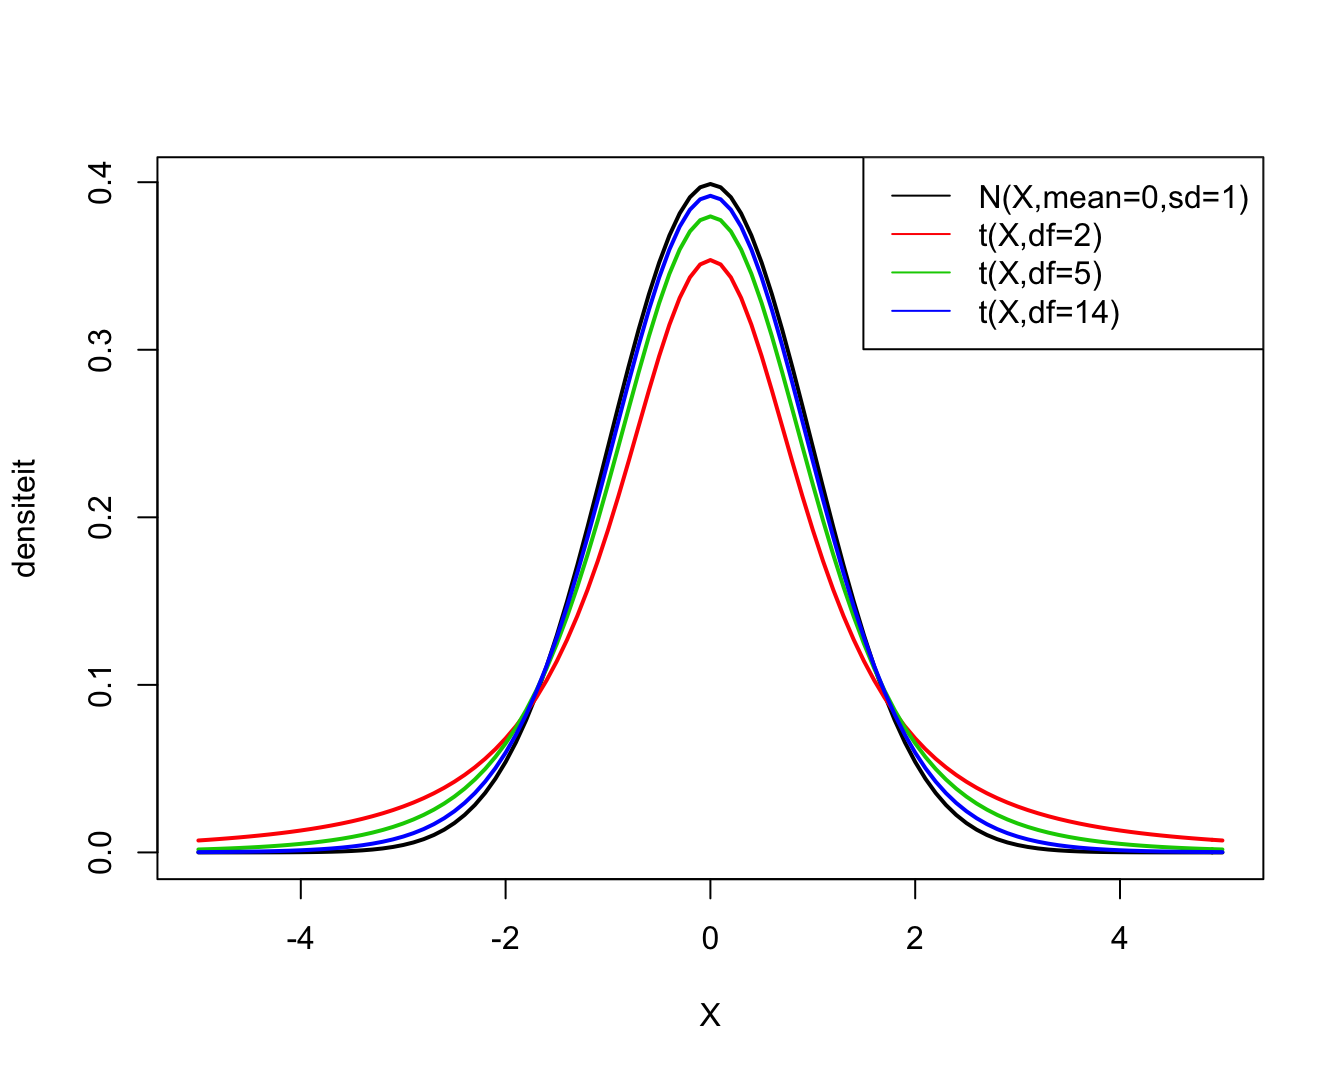
\includegraphics[width=1\linewidth]{Statistiek_2019_2020_files/figure-latex/tdist-1} 

}

\caption{Normale verdeling en t-verdeling met verschillende vrijheidsgraden.}\label{fig:tdist}
\end{figure}

Percentielen van de \(t\)-verdeling kunnen niet met de hand berekend
worden, maar kan men voor de verschillende waarden van \(n\) aflezen in
Tabellen of berekenen in R. In de onderstaande code wordt het 95\%,
97.5\%, 99.5\% percentiel berekend voor een t-verdeling met 14
vrijheidsgraden, die gebruik kunnen worden voor de berekening van 90\%,
95\% en 99\% betrouwbaarheidsintervallen.

\begin{Shaded}
\begin{Highlighting}[]
\KeywordTok{qt}\NormalTok{(}\FloatTok{0.975}\NormalTok{, }\DataTypeTok{df =} \DecValTok{14}\NormalTok{)}
\end{Highlighting}
\end{Shaded}

\begin{verbatim}
## [1] 2.144787
\end{verbatim}

\begin{Shaded}
\begin{Highlighting}[]
\KeywordTok{qt}\NormalTok{(}\KeywordTok{c}\NormalTok{(}\FloatTok{0.95}\NormalTok{, }\FloatTok{0.975}\NormalTok{, }\FloatTok{0.995}\NormalTok{), }\DataTypeTok{df =} \DecValTok{14}\NormalTok{)}
\end{Highlighting}
\end{Shaded}

\begin{verbatim}
## [1] 1.761310 2.144787 2.976843
\end{verbatim}

We zien dat het 97.5\% percentiel 2.14 voor een t-verdeling met
\(n-1=14\) vrijheidsgraden inderdaad groter is dan het kwantiel uit de
normaal verdeling 1.96.

Een gelijkaardige logica als voor de Normale verdeling met gekende
variantie, geeft dan aan dat een \(100\% (1-\alpha)\)
betrouwbaarheidsinterval voor het gemiddelde \(\mu\) van een Normaal
verdeelde veranderlijke \(X\) met onbekende variantie kan berekend
worden als

\begin{equation*}
\left[\bar{X} - t_{n-1, \alpha/2} \frac{s}{\sqrt{n}} , \bar{X} + t_{n-1,
\alpha/2} \frac{s}{\sqrt{n}}\right]
\end{equation*}

Deze uitdrukking verschilt van deze in de vorige sectie doordat het
\((1-\alpha/2)100\%\) percentiel van de Normale verdeling wordt
vervangen door het \((1-\alpha/2)100\%\) percentiel van de t-verdeling
met \(n-1\) vrijheidsgraden.

Voor het captopril voorbeeld kunnen we dus een 95\%
betrouwbaarheidsinterval bekomen door

\begin{Shaded}
\begin{Highlighting}[]
\KeywordTok{mean}\NormalTok{(delta) }\OperatorTok{-}\StringTok{ }\KeywordTok{qt}\NormalTok{(}\FloatTok{0.975}\NormalTok{, }\DataTypeTok{df =} \DecValTok{14}\NormalTok{) }\OperatorTok{*}\StringTok{ }\KeywordTok{sd}\NormalTok{(delta)}\OperatorTok{/}\KeywordTok{sqrt}\NormalTok{(n)}
\end{Highlighting}
\end{Shaded}

\begin{verbatim}
## [1] -23.93258
\end{verbatim}

\begin{Shaded}
\begin{Highlighting}[]
\KeywordTok{mean}\NormalTok{(delta) }\OperatorTok{+}\StringTok{ }\KeywordTok{qt}\NormalTok{(}\FloatTok{0.975}\NormalTok{, }\DataTypeTok{df =} \DecValTok{14}\NormalTok{) }\OperatorTok{*}\StringTok{ }\KeywordTok{sd}\NormalTok{(delta)}\OperatorTok{/}\KeywordTok{sqrt}\NormalTok{(n)}
\end{Highlighting}
\end{Shaded}

\begin{verbatim}
## [1] -13.93409
\end{verbatim}

Een 99\% betrouwbaarheidsinterval voor gemiddelde bloeddrukverandering
wordt als volgt bekomen:

\begin{Shaded}
\begin{Highlighting}[]
\KeywordTok{mean}\NormalTok{(delta) }\OperatorTok{-}\StringTok{ }\KeywordTok{qt}\NormalTok{(}\FloatTok{0.995}\NormalTok{, }\DataTypeTok{df =} \DecValTok{14}\NormalTok{) }\OperatorTok{*}\StringTok{ }\KeywordTok{sd}\NormalTok{(delta)}\OperatorTok{/}\KeywordTok{sqrt}\NormalTok{(n)}
\end{Highlighting}
\end{Shaded}

\begin{verbatim}
## [1] -25.87201
\end{verbatim}

\begin{Shaded}
\begin{Highlighting}[]
\KeywordTok{mean}\NormalTok{(delta) }\OperatorTok{+}\StringTok{ }\KeywordTok{qt}\NormalTok{(}\FloatTok{0.995}\NormalTok{, }\DataTypeTok{df =} \DecValTok{14}\NormalTok{) }\OperatorTok{*}\StringTok{ }\KeywordTok{sd}\NormalTok{(delta)}\OperatorTok{/}\KeywordTok{sqrt}\NormalTok{(n)}
\end{Highlighting}
\end{Shaded}

\begin{verbatim}
## [1] -11.99466
\end{verbatim}

\subsection{Interpretatie van
betrouwbaarheidsintervallen}\label{subsec:interpretBI}

We zullen de interpretatie van betrouwbaarheidsintervallen weergegeven
a.d.h.v. een simulatie studie waarbij we 1000 herhaalde steekproeven
simuleren met 15 observaties uit een normaal verdeling. De gemiddelde
bloeddrukdaling in de populatie bedraagt -18.9 mmHg en de
standaarddeviate 9.0 mmHg. We houden voor elke steekproef volgende
gegevens bij: het gemiddelde, de ondergrens en bovengrens van het BI en
of het BI het werkelijke gemiddelde.

\begin{Shaded}
\begin{Highlighting}[]
\KeywordTok{set.seed}\NormalTok{(}\DecValTok{115}\NormalTok{)}
\NormalTok{mu <-}\StringTok{ }\OperatorTok{-}\FloatTok{18.9}
\NormalTok{sigma <-}\StringTok{ }\DecValTok{9}
\NormalTok{nSim <-}\StringTok{ }\DecValTok{1000}
\NormalTok{alpha <-}\StringTok{ }\FloatTok{0.05}
\NormalTok{n <-}\StringTok{ }\DecValTok{15}
\NormalTok{muHat <-}\StringTok{ }\NormalTok{sigmaHat <-}\StringTok{ }\NormalTok{BI.ondergrens <-}\StringTok{ }\NormalTok{BI.bovengrens <-}\StringTok{ }\NormalTok{omvat <-}\StringTok{ }\KeywordTok{array}\NormalTok{(}\DataTypeTok{dim =}\NormalTok{ nSim)}
\NormalTok{cnt <-}\StringTok{ }\DecValTok{0}
\ControlFlowTok{for}\NormalTok{ (i }\ControlFlowTok{in} \DecValTok{1}\OperatorTok{:}\NormalTok{nSim) \{}
\NormalTok{    y <-}\StringTok{ }\KeywordTok{rnorm}\NormalTok{(n, }\DataTypeTok{mean =}\NormalTok{ mu, }\DataTypeTok{sd =}\NormalTok{ sigma)}
\NormalTok{    muHat[i] <-}\StringTok{ }\KeywordTok{mean}\NormalTok{(y)}
\NormalTok{    sigmaHat[i] <-}\StringTok{ }\KeywordTok{sd}\NormalTok{(y)}\OperatorTok{/}\KeywordTok{sqrt}\NormalTok{(n)}
\NormalTok{    BI.ondergrens[i] <-}\StringTok{ }\NormalTok{muHat[i] }\OperatorTok{-}\StringTok{ }\KeywordTok{qt}\NormalTok{(}\DecValTok{1} \OperatorTok{-}\StringTok{ }\NormalTok{alpha}\OperatorTok{/}\DecValTok{2}\NormalTok{, }
        \DataTypeTok{df =}\NormalTok{ n }\OperatorTok{-}\StringTok{ }\DecValTok{1}\NormalTok{) }\OperatorTok{*}\StringTok{ }\NormalTok{sigmaHat[i]}
\NormalTok{    BI.bovengrens[i] <-}\StringTok{ }\NormalTok{muHat[i] }\OperatorTok{+}\StringTok{ }\KeywordTok{qt}\NormalTok{(}\DecValTok{1} \OperatorTok{-}\StringTok{ }\NormalTok{alpha}\OperatorTok{/}\DecValTok{2}\NormalTok{, }
        \DataTypeTok{df =}\NormalTok{ n }\OperatorTok{-}\StringTok{ }\DecValTok{1}\NormalTok{) }\OperatorTok{*}\StringTok{ }\NormalTok{sigmaHat[i]}
\NormalTok{    omvat[i] <-}\StringTok{ }\NormalTok{(mu }\OperatorTok{<}\StringTok{ }\NormalTok{BI.bovengrens[i]) }\OperatorTok{&}\StringTok{ }\NormalTok{(BI.ondergrens[i] }\OperatorTok{<}\StringTok{ }
\StringTok{        }\NormalTok{mu)}
\NormalTok{    cnt <-}\StringTok{ }\NormalTok{cnt }\OperatorTok{+}\StringTok{ }\KeywordTok{as.numeric}\NormalTok{(omvat[i])}
\NormalTok{\}}
\NormalTok{cnt}\OperatorTok{/}\NormalTok{nSim}
\end{Highlighting}
\end{Shaded}

\begin{verbatim}
## [1] 0.951
\end{verbatim}

Op basis van de 1000 herhaalde steekproeven van de simulatiestudie zien
we dat voor 95.1\% van de steekproeven de intervallen het werkelijke
populatiegemiddelde bevat\footnote{95.1\% is niet exact gelijk aan het
  nominale 95\% omdat er `slechts' 1000 simulaties gelopen zijn}. De
simulatiestudie toont dus op een empirische wijze aan dat de constructie
correct is. Het demonstreert bovendien de interpretatie van
probabiliteit via herhaalde steekproefname. In Figuur
\ref{fig:biInterpret} wordt de interpretatie ook grafisch weergegeven
voor de eerste 100 gesimuleerde steekproeven. De figuur toont duidelijk
aan dat het werkelijke populatiegemiddelde vast is maar ongekend. Het
wordt geschat aan de hand van het steekproefgemiddelde dat at random
varieert van steekproef tot steekproef rond het werkelijk gemiddelde. We
zien ook dat de grenzen van de betrouwbaarheidsintervallen variëren van
steekproef tot steekproef. Daarnaast varieert de breedte van de
betrouwbaarheidsintervallen eveneens omdat de
steekproefstandaarddeviatie eveneens varieert van steekproef tot
steekproef\footnote{De steekproefstandaarddeviatie is eveneens een
  toevallig veranderlijke die van steekproef tot steekproef varieert
  rond werkelijke standaarddeviatie. Hierdoor zal de breedte van de
  intervallen eveneens variëren}.

In de praktijk zullen we op basis van 1 steekproef besluiten dat het
betrouwbaarheidsinterval het populatiegemiddelde bevat en we weten dat
dergelijke uitspraken met een kans van \(1-\alpha\) (hier 95\%) correct
zijn.

\begin{figure}

{\centering 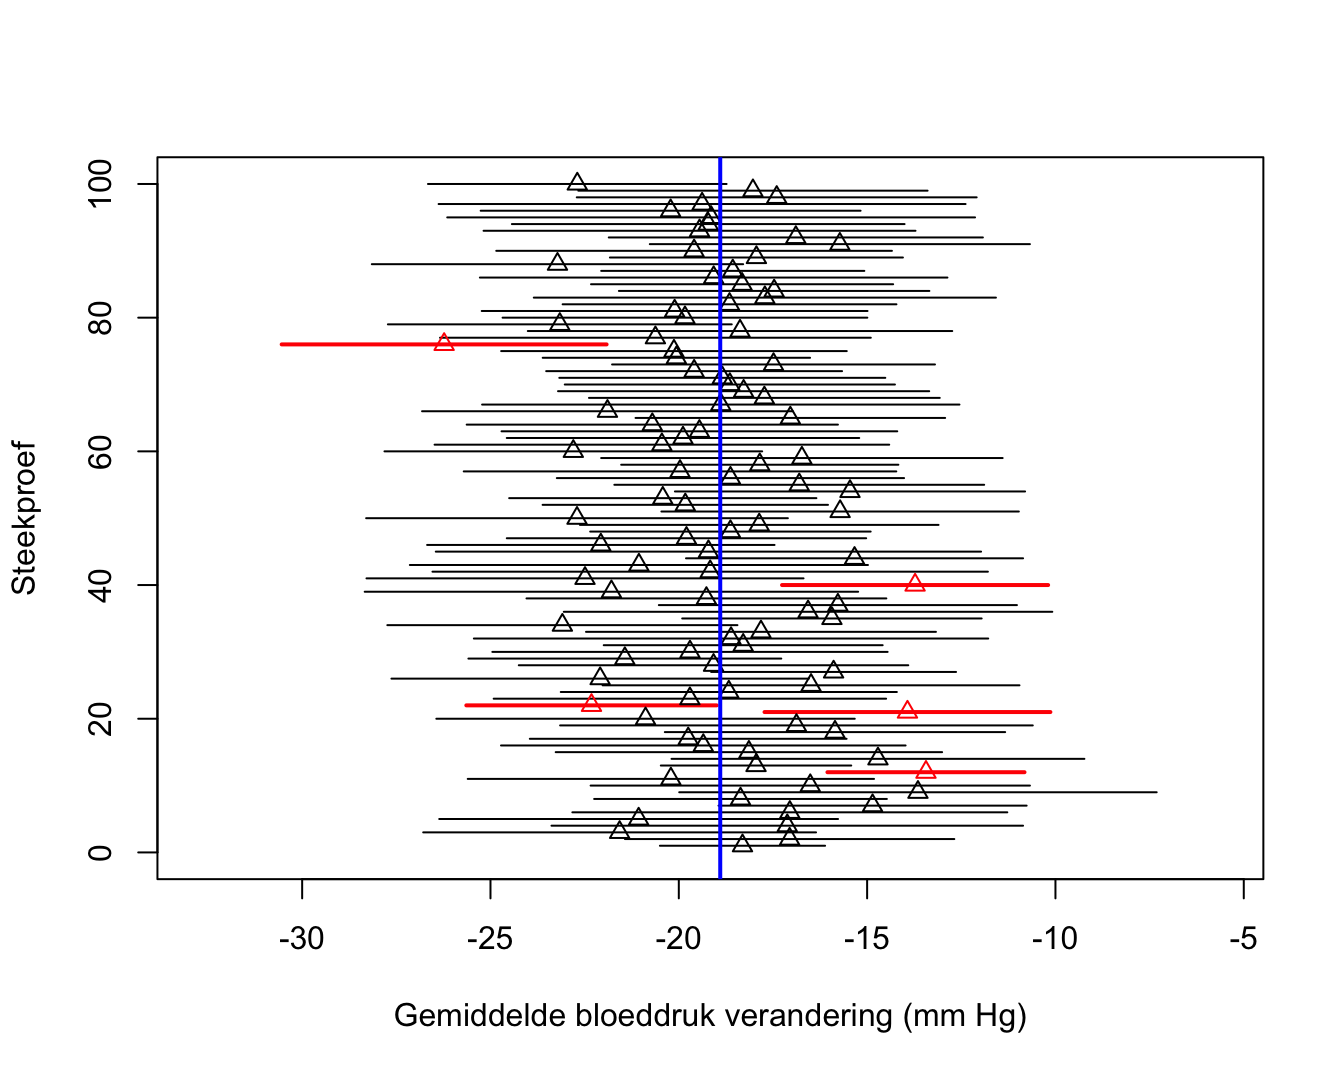
\includegraphics[width=1\linewidth]{Statistiek_2019_2020_files/figure-latex/biInterpret-1} 

}

\caption{Interpretatie van 95$\%$ betrouwbaarheidintervallen. Resultaten op basis van 100 gesimuleerde steekproeven. We zien in de figuur duidelijk dat het populatiegemiddelde vast is maar ongekend (blauwe lijn) en dat de bovengrens en ondergrens van betrouwbaarheidsintervallen voor het populatiegemiddelde varieert van steekproef tot steekproef. Van de 100 betrouwbaarheidsintervallen die worden geplot bevatten 95 intervallen het werkelijke steekproef gemiddelde (zwarte BIs). Voor 5 intervallen is dat niet het geval (rode BIs).}\label{fig:biInterpret}
\end{figure}

We zullen nu de simulatie herhalen, maar zullen het aantal observaties
in de steekproef verdubbelen.

\begin{Shaded}
\begin{Highlighting}[]
\NormalTok{mu <-}\StringTok{ }\OperatorTok{-}\FloatTok{18.9}
\NormalTok{sigma <-}\StringTok{ }\DecValTok{9}
\NormalTok{nSim <-}\StringTok{ }\DecValTok{1000}
\NormalTok{alpha <-}\StringTok{ }\FloatTok{0.05}
\NormalTok{n <-}\StringTok{ }\DecValTok{30}
\NormalTok{muHat <-}\StringTok{ }\NormalTok{sigmaHat <-}\StringTok{ }\NormalTok{BI.ondergrens <-}\StringTok{ }\NormalTok{BI.bovengrens <-}\StringTok{ }\NormalTok{omvat <-}\StringTok{ }\KeywordTok{array}\NormalTok{(}\DataTypeTok{dim =}\NormalTok{ nSim)}
\NormalTok{cnt <-}\StringTok{ }\DecValTok{0}
\ControlFlowTok{for}\NormalTok{ (i }\ControlFlowTok{in} \DecValTok{1}\OperatorTok{:}\NormalTok{nSim) \{}
\NormalTok{    y <-}\StringTok{ }\KeywordTok{rnorm}\NormalTok{(n, }\DataTypeTok{mean =}\NormalTok{ mu, }\DataTypeTok{sd =}\NormalTok{ sigma)}
\NormalTok{    muHat[i] <-}\StringTok{ }\KeywordTok{mean}\NormalTok{(y)}
\NormalTok{    sigmaHat[i] <-}\StringTok{ }\KeywordTok{sd}\NormalTok{(y)}\OperatorTok{/}\KeywordTok{sqrt}\NormalTok{(n)}
\NormalTok{    BI.ondergrens[i] <-}\StringTok{ }\NormalTok{muHat[i] }\OperatorTok{-}\StringTok{ }\KeywordTok{qt}\NormalTok{(}\DecValTok{1} \OperatorTok{-}\StringTok{ }\NormalTok{alpha}\OperatorTok{/}\DecValTok{2}\NormalTok{, }
        \DataTypeTok{df =}\NormalTok{ n }\OperatorTok{-}\StringTok{ }\DecValTok{1}\NormalTok{) }\OperatorTok{*}\StringTok{ }\NormalTok{sigmaHat[i]}
\NormalTok{    BI.bovengrens[i] <-}\StringTok{ }\NormalTok{muHat[i] }\OperatorTok{+}\StringTok{ }\KeywordTok{qt}\NormalTok{(}\DecValTok{1} \OperatorTok{-}\StringTok{ }\NormalTok{alpha}\OperatorTok{/}\DecValTok{2}\NormalTok{, }
        \DataTypeTok{df =}\NormalTok{ n }\OperatorTok{-}\StringTok{ }\DecValTok{1}\NormalTok{) }\OperatorTok{*}\StringTok{ }\NormalTok{sigmaHat[i]}
\NormalTok{    omvat[i] <-}\StringTok{ }\NormalTok{(mu }\OperatorTok{<}\StringTok{ }\NormalTok{BI.bovengrens[i]) }\OperatorTok{&}\StringTok{ }\NormalTok{(BI.ondergrens[i] }\OperatorTok{<}\StringTok{ }
\StringTok{        }\NormalTok{mu)}
\NormalTok{    cnt <-}\StringTok{ }\NormalTok{cnt }\OperatorTok{+}\StringTok{ }\KeywordTok{as.numeric}\NormalTok{(omvat[i])}
\NormalTok{\}}
\NormalTok{cnt}\OperatorTok{/}\NormalTok{nSim}
\end{Highlighting}
\end{Shaded}

\begin{verbatim}
## [1] 0.949
\end{verbatim}

We zien een coverage van 94.9\% wat opnieuw dicht ligt bij de nominale
coverage van 95\%.

Wanneer we opnieuw de eerste 100 betrouwbaarheidsintervallen plotten
(Figuur \ref{fig:biInterpretLargeSample}) merken we op dat de
intervallen smaller zijn dan in Figuur \ref{fig:biInterpret} (waarom is
dat het geval, ga zelf na met welke factor de intervallen ongeveer
versmallen?)

\begin{figure}

{\centering 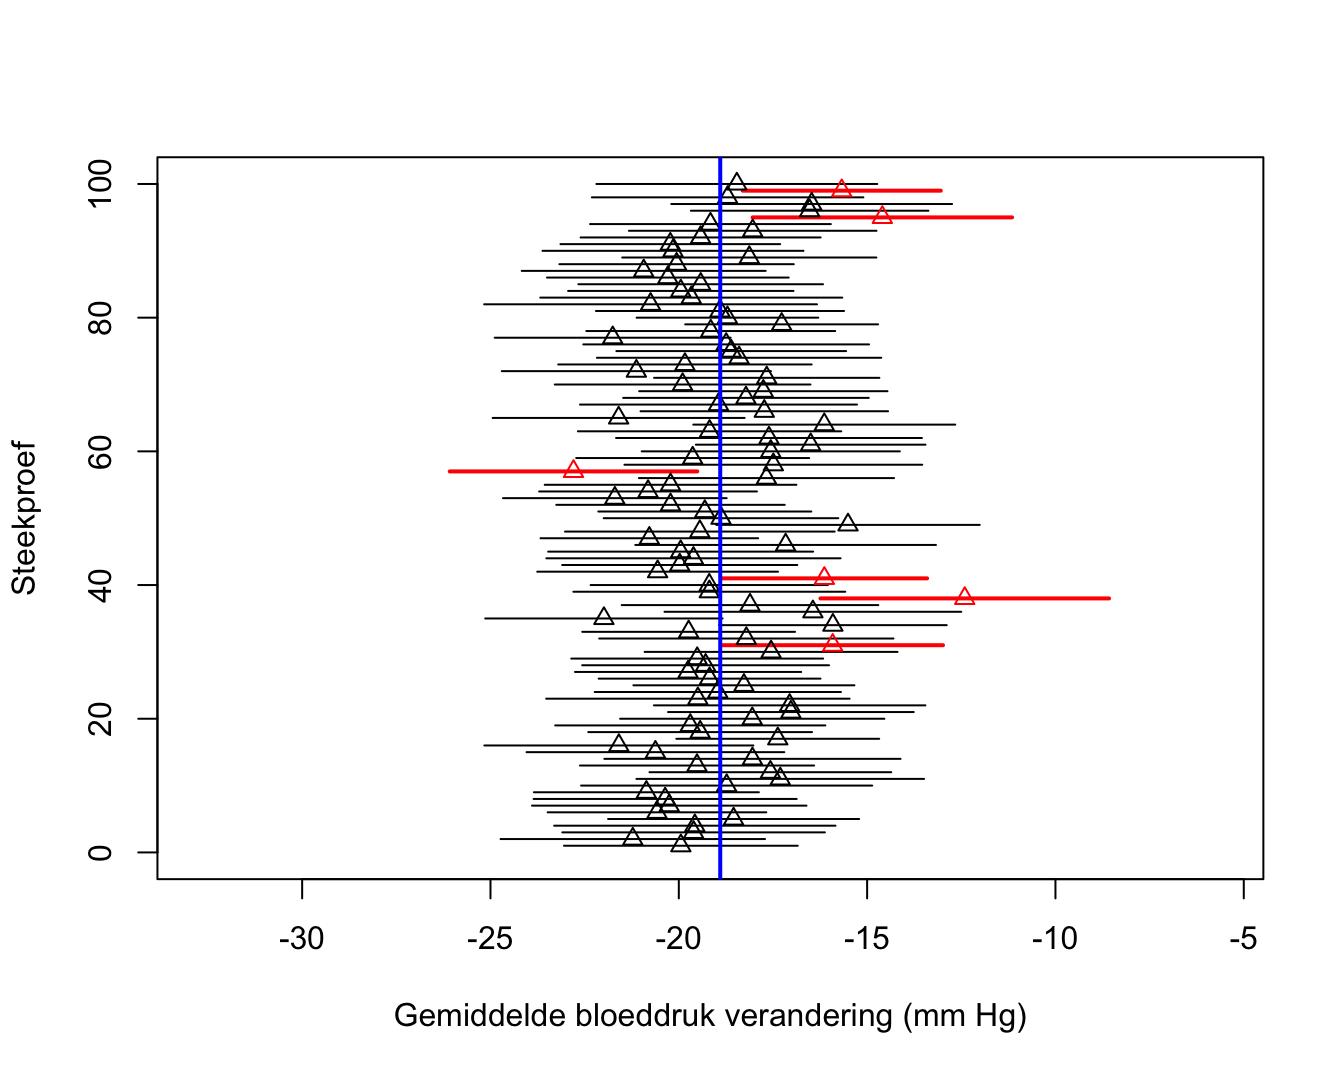
\includegraphics[width=1\linewidth]{Statistiek_2019_2020_files/figure-latex/biInterpretLargeSample-1} 

}

\caption{Interpretatie van 95$\%$ betrouwbaarheidintervallen. Resultaten op basis van 100 gesimuleerde steekproeven. We zien in de figuur duidelijk dat het populatiegemiddelde vast is maar ongekend (blauwe lijn) en dat de bovengrens en ondergrens van betrouwbaarheidsintervallen voor het populatiegemiddelde varieert van steekproef tot steekproef. Van de 100 betrouwbaarheidsintervallen die worden geplot bevatten 95 intervallen het werkelijke steekproef gemiddelde (zwarte BIs). Voor 5 intervallen is dat niet het geval (rode BIs).}\label{fig:biInterpretLargeSample}
\end{figure}

\subsection{Wat rapporteren?}\label{wat-rapporteren}

Rapporteer dus zeker steeds de onzekerheid op de resultaten! Conclusies
trekken op basis van 1 schatting kan zeer misleidend zijn! In
statistische analyses rapporteert men daarom systematisch
betrouwbaarheidsintervallen. Betrouwbaarheidsintervallen vormen een goed
compromis: ze zijn smal genoeg om informatief te zijn, maar haast nooit
zeer misleidend. We besluiten dat de parameter die ons interesseert in
het 95\% betrouwbaarheidsinterval zit, en weten dat die uitspraak met
95\% kans correct is. In de statistiek trekt men dus nooit absolute
conclusies.

Op basis van de data-analyse voor het captopril voorbeeld kunnen we dus
besluiten dat de gemiddelde bloeddrukdaling 18.9mmHg bedraagt na het
toedienen van captopril. Met een 95\% betrouwbaarheidsinterval op het
gemiddelde van {[}-22.3,-15.6{]}mmHg. Op basis van het
betrouwbaarheidsinterval is het duidelijk dat het toedienen van
captopril resulteert in een sterke bloeddrukdaling bij patiënten met
hypertensie.

\section{Principe van Hypothesetoetsen (via one sample
t-test)}\label{principe-van-hypothesetoetsen-via-one-sample-t-test}

We wensen een uitspraak te kunnen doen of er al dan niet een effect is
van het toedienen van Captopril op de systolische bloeddruk? Beslissen
op basis van gegevens is niet evident. Er is immers onzekerheid of de
bevindingen uit de steekproef generaliseerbaar zijn naar de populatie.
We stellen ons dus de vraag of het schijnbaar gunstig effect
systematisch of toevallig is? Een natuurlijke beslissingsbasis is het
gemiddeld verschil \(X\) in de systolische bloeddruk:

\(\bar x=\) -18.93mmHg (\(s =\) 9.03, \(SE =\) 2.33).

Dat \(\bar{x}< 0\) volstaat niet om te beslissen dat de gemiddelde
systolische bloeddruk lager is na het toedienen van captopril \emph{op
het niveau van de volledige populatie}. Om het effect die we in de
steekproef observeren te kunnen \emph{veralgemenen} naar de populatie
moet de bloeddrukverlaging voldoende groot zijn. Maar hoe groot moet dit
effect nu zijn?

Hiervoor hebben statistici zogenaamde \emph{toetsen} ontwikkeld om met
dit soort vragen om te gaan. Deze leveren een ja/nee antwoord op de
vraag of een geobserveerde associatie systematisch is (d.w.z. opgaat
voor de studiepopulatie) of als er integendeel onvoldoende informatie in
de steekproef voorhanden is om te besluiten dat de geobserveerde
associatie ook aanwezig is in de volledige studiepopulatie. Tegenwoordig
is het haast onmogelijk om een wetenschappelijk onderzoeksartikel te
lezen zonder de resultaten van dergelijke toetsen te ontmoeten. Om die
reden wensen we in dit hoofdstuk in te gaan op de betekenis van
statistische toetsen en hun nomenclatuur.

We weten dat we volgens het \emph{falcificatieprincipe} van Popper nooit
een hypothese kunnen bewijzen op basis van data (zie Sectie
\ref{sec:wetMeth}). Daarom zullen we twee hypotheses introduceren: een
nulhypothese en een alternatieve hypothese. We zullen dan later a.d.h.v.
de toets de nulhypothese trachten te ontkrachten.

\subsection{Hypotheses}\label{hypotheses}

Algemeen starten we met het vertalen van de wetenschappelijke
vraagstelling naar een nulhypothese (\(H_0\)) en een alternatieve
hypothese (\(H_1\)). Dit kan pas nadat de probleemstelling vertaald is
naar een geparametriseerd statistisch model. Uit de beschrijving van de
proefopzet volgt dat \(X_1,...,X_n\) i.i.d.\footnote{independent and
  identically distributed, onafhankelijk en gelijk verdeeld} \(f(X)\)
met \(f(X)\) de dichtheidsfunctie van de bloeddrukverschillen.

\textbf{Vereenvoudiging}: veronderstel dat \(f(X)\) gekend is op een
eindig-dimensionale set van parameters \(\mathbf{\theta}\) na
(parametrisch statistisch model). Voor het captopril voorbeeld
veronderstellen we dat \(f(X)\) een normale distributie
\(N(\mu,\sigma^2)\) volgt met parameters
\(\mathbf{\theta}=(\mu,\sigma^2)\), het gemiddelde \(\mu\) en variantie
\(\sigma^2\).

De vraagstelling is geformuleerd in termen van de gemiddelde
bloeddrukdaling: \(\mu=E_f[X]\).

De \textbf{alternatieve hypothese} wordt geformuleerd in termen van een
parameter van \(f(X)\) en dient uit te drukken wat de onderzoekers
wensen te bewijzen aan de hand van de studie. Hier: \[H_1: \mu<0.\]
Gemiddeld gezien daalt de bloeddruk bij patiënten met hypertensie na
toediening van captopril.

De \textbf{nulhypothese} is meestal een uitdrukking van de nultoestand,
i.e.~de omstandigheden waarin niets bijzonders aan de hand is. De
onderzoekers wensen meestal te bewijzen via empirisch onderzoek dat de
nulhypothese niet waar is: \textbf{Falsificatie principe}. De
\textbf{nulhypothese wordt veelal uitgedrukt door gebruik te maken van
dezelfde parameter als deze die in \(H_1\)} gebruikt is. Hier:
\[H_0 : \mu=0\] m.a.w. gemiddeld gezien blijft de systolische bloeddruk
na toediening van captopril onveranderd.

\subsection{Test-statistiek}\label{test-statistiek}

Eens de populatie, de parameters en de nulhypothese en alternatieve
hypothese bepaald zijn, kan de basisgedachte van een hypothesetest als
volgt bondig beschreven worden.

Construeer een teststatistiek zodanig dat deze

\begin{enumerate}
\def\labelenumi{\arabic{enumi}.}
\tightlist
\item
  de evidentie meet die aanwezig is in de steekproef,
\item
  tegen de gestelde nulhypothese,
\item
  ten voordele van de alternatieve hypothese.
\end{enumerate}

Een teststatistiek is dus noodzakelijk een functie van de
steekproefobservaties.

Voor het captopril voorbeeld drukt de statistiek \[T=\bar X - \mu_0\]
uit hoever het steekproefgemiddelde van de bloeddrukdaling ligt van het
gemiddelde \(\mu_0=0\) in de populatie onder de nulhypothese\footnote{vandaar
  de index 0 bij \(\mu_0\)}.

\begin{itemize}
\tightlist
\item
  Als \(H_0\) waar is en er dus geen effect is van captopril in de
  populatie, dan verwachten we dat de teststatistiek T dicht ligt bij
  \(T=0\)
\item
  Als \(H_1\) waar is, dan verwachten we dat \(T<0\).
\end{itemize}

In de praktijk gebruiken we echter meestal teststatistieken die niet
alleen de grootte van het effect in rekening brengen maar ook de
onzekerheid op het effect. We doen dit door de effectgrootte te
balanceren t.o.v. de standard error.

\[T=\frac{\bar{X}-0}{\text{SE}_{\bar X}}\] Waarbij \(\mu_0=0\) voor het
captopril voorbeeld.

Opnieuw geldt dat

\begin{itemize}
\tightlist
\item
  Als \(H_0\) waar is en er dus geen effect is van captopril in de
  populatie, dan verwachten we dat de teststatistiek T dicht ligt bij
  \(T=0\)
\item
  Als \(H_1\) waar is, dan verwachten we dat \(T<0\).
\item
  Voor het captopril voorbeeld vinden we \(t=(-18.93-0)/2.33=-8.12\).
\item
  Is \(t = -8.12\) groot genoeg in absolute waarde om te kunnen
  besluiten dat \(\mu < 0\) en met welke zekerheid kunnen we dit
  besluiten?
\end{itemize}

Om daar een uitspraak over te doen zullen we de teststatistiek T verder
bestuderen. T is een toevalsveranderlijke en de verdeling van T hangt af
van de verdeling van de steekproefobservaties, maar die verdeling is
ongekend! We hebben normaliteit verondersteld, maar dit laat nog steeds
het gemiddelde en de variantie onbepaald. Bovendien wordt de
hypothesetest net geconstrueerd om een uitspraak te kunnen doen over het
gemiddelde \(\mu\)! De oplossing zit in de nulhypothese die we kunnen
veronderstellen als er geen effect is van captopril. De \(H_0\) stelt
dat \(\mu=0\). Als we aannemen dat \(H_0\) waar is, dan is het
gemiddelde van de normale distributie gekend! Als de
bloeddrukverschillen \(X_1, \ldots X_{15}\) onafhankelijk en identiek
normaal verdeeld (i.i.d.) zijn, dan weten we dat
\[\bar X  \stackrel{H_0}{\sim} N(0, \sigma^2/n)\]

Gezien we \(\sigma^2\) niet kennen kunnen we deze vervangen door de
steekproef variantie. Dan weten we dat
\[T=\frac{\bar{X}-0}{\text{SE}_{\bar X}}\stackrel{H_0}{\sim} t(n-1) \]
een t-verdeling volgt met n-1 vrijheidsgraden onder de
\textbf{nulhypothese}. We weten dat indien de alternatieve hypothese
waar zou zijn, we mogen verwachten dat er meer kans is op het observeren
van een kleine waarde voor de teststatistiek dan wat verwacht wordt
onder de nulhypothese. We zullen de verdeling van de teststatistiek
onder de nulhypothese gebruiken om na te gaan of de geobserveerde
test-statistiek \(t = -8.12\) klein genoeg is om te kunnen besluiten dat
\(\mu < 0\).

\begin{itemize}
\tightlist
\item
  \textbf{Is de geobserveerde teststatistiekwaarde (\(t=-8.12\)) een
  waarde die we verwachten als \(H_0\) waar is}, of is het een waarde
  die onwaarschijnlijk klein is als \(H_0\) waar is?
\item
  In het laatste geval deduceren we dat we niet langer kunnen aannemen
  dat \(H_0\) waar is, en dienen we dus \(H_1\) te concluderen.
\item
  De vraag blijft: (a) hoe groot moet de geobserveerde teststatistiek
  \(t\) zijn opdat we \(H_0\) verwerpen zodat (b) we bereid zijn om
  \(H_1\) te besluiten en (c) hoe zeker zijn we van deze beslissing?
\item
  Het antwoord hangt samen met de interpretatie van de kansen die
  berekend kunnen worden op basis van de nuldistributie\footnote{distributie
    van de teststatistiek onder de nulhypothese} en de geobserveerde
  teststatistiek \(t\).
\end{itemize}

\subsection{De p-waarde}\label{de-p-waarde}

De kans waarop de keuze tussen \(H_0\) en \(H_1\) gebaseerd wordt, wordt
de \textbf{\(p\)-waarde} genoemd. De berekeningswijze is
context-afhankelijk, maar voor het huidige voorbeeld wordt de
\(p\)-waarde gegeven door \[
    p = P\left[T \leq t \mid H_0\right] = \text{P}_0\left[T\leq t\right],
  \] waar de index ``0'' in \(\text{P}_0\left[.\right]\) aangeeft dat de
kans onder de nulhypothese berekend wordt. Het is met andere woorden de
kans om in een willekeurige steekproef onder de nulhypothese een waarde
voor de teststatistiek T te bekomen die lager of gelijk is aan\footnote{meer
  extreem in de richting van \(H_1\)} de waarde die in de huidige
steekproef werd geobserveerd.

De \(p\)-waarde voor het captopril voorbeeld wordt berekend als
\[p= \text{P}_0\left[T\leq -8.12\right]=F_t(-8.12;14) = 0.6\ 10^{-6}.\]

waarbij \(F_t(;14)\) de cumulatieve distributie functie is van een
t-verdeling met 14 vrijheidsgraden,
\[F_t(x;14)=\int\limits_{-\infty}^{x} f_t(x;14).\] Waarbij \(f_t(.;14)\)
de densiteitsfunctie is van de t-verdeling. De oppervlakte onder de
densiteitsfunctie is opnieuw een kans. Deze kans kan berekend worden in
R m.b.v. de functie \texttt{pt(x,df)} die twee argumenten heeft, de
waarde van de test-statistiek \texttt{x} en het aantal vrijheidsgraden
van de t-verdeling \texttt{df}. \texttt{pt(x,df)} berekent de kans om
een waarde te observeren die kleiner of gelijk is aan x wanneer men een
willekeurige observatie trekt uit een t-verdeling met df
vrijheidsgraden.

\begin{Shaded}
\begin{Highlighting}[]
\NormalTok{n <-}\StringTok{ }\KeywordTok{length}\NormalTok{(delta)}
\NormalTok{stat <-}\StringTok{ }\NormalTok{(}\KeywordTok{mean}\NormalTok{(delta) }\OperatorTok{-}\StringTok{ }\DecValTok{0}\NormalTok{)}\OperatorTok{/}\NormalTok{(}\KeywordTok{sd}\NormalTok{(delta)}\OperatorTok{/}\KeywordTok{sqrt}\NormalTok{(n))}
\NormalTok{stat}
\end{Highlighting}
\end{Shaded}

\begin{verbatim}
## [1] -8.122816
\end{verbatim}

\begin{Shaded}
\begin{Highlighting}[]
\KeywordTok{pt}\NormalTok{(stat, n }\OperatorTok{-}\StringTok{ }\DecValTok{1}\NormalTok{)}
\end{Highlighting}
\end{Shaded}

\begin{verbatim}
## [1] 5.731936e-07
\end{verbatim}

\BeginKnitrBlock{definition}[$p$-waarde]
\protect\hypertarget{def:unnamed-chunk-80}{}{\label{def:unnamed-chunk-80}
\iffalse (\(p\)-waarde) \fi{} }De \textbf{p-waarde} (ook wel
\textbf{geobserveerd significantieniveau} genoemd) is de kans om onder
de nulhypothese een even of meer ``extreme'' toetsinggrootheid waar te
nemen (in de richting van het alternatief) dan de waarde \(t\) die
geobserveerd werd o.b.v. de steekproef. Hoe kleiner die kans is, hoe
sterker het bewijs tegen de nulhypothese.

Merk op dat de p-waarde de kans \textbf{niet} uitdrukt dat de
nulhypothese waar is!\footnote{In de frequentistische theorie die we
  hier volgen, is de nulhypothese immers ofwel altijd waar, ofwel altijd
  vals, en is het dus zelfs niet mogelijk om de kans te definiëren dat
  de nulhypothese waar is. Teminste, die kans is ofwel 1 ofwel 0.!}.

\textbf{Einde Definitie}
\EndKnitrBlock{definition}

Het woord ``extreem'' duidt op de richting waarvoor de teststatistiek
onder de alternatieve hypothese meer waarschijnlijk is. In het voorbeeld
is \(H_1: \mu < 0\) en verwachten we dus kleinere waarden van \(t\)
onder \(H_1\). Vandaar de kans op \(T\leq t\). Uit de definitie van de
\(p\)-waarde volgt dat een kleine \(p\)-waarde betekent dat de
geobserveerde teststatistiek eerder onwaarschijnlijk is als aangenomen
wordt dat \(H_0\) correct is. Dus een voldoende kleine \(p\)-waarde
noopt ons tot het \textbf{verwerpen van \(H_0\)} ten voordele van
\(H_1\). De drempelwaarde waarmee de \(p\)-waarde vergeleken wordt,
wordt het \textbf{significanctieniveau} genoemd en wordt voorgesteld
door \(\alpha\).

\BeginKnitrBlock{definition}[significantieniveau]
\protect\hypertarget{def:unnamed-chunk-81}{}{\label{def:unnamed-chunk-81}
\iffalse (significantieniveau) \fi{} }De drempelwaarde \(\alpha\) staat
gekend als het \textbf{significantieniveau} van de statistische test.
Een statistische test uitgevoerd op het \(\alpha\) significantieniveau
wordt een \textbf{niveau-\(\alpha\) test} genoemd (Engels:
\emph{level-\(\alpha\) test}).

\textbf{Einde definitie}
\EndKnitrBlock{definition}

Een toetsingsresultaat wordt \emph{statistisch significant} genoemd
wanneer de bijhorende p-waarde kleiner is dan \(\alpha\), waarbij
\(\alpha\) meestal gelijk aan 5\% wordt genomen. Hoe kleiner de p-waarde
hoe meer `significant' het testresultaat afwijkt van de verwachting
onder de nulhypothese. Het aangeven van een p-waarde voor een toets
geeft bijgevolg meer informatie over het resultaat dan een eenvoudig
ja/nee antwoord of de nulhypothese wordt verworpen op een vast gekozen
\(\alpha\)-niveau. Het geeft immers niet alleen aan of de nulhypothese
verworpen wordt op een gegeven significantieniveau, maar ook op welke
significantieniveaus de nulhypothese verworpen wordt.

Ze vat dus de bewijskracht tegen de nulhypothese samen
\[\begin{array}{cl}>0.10 & \text{ niet significant (zwak bewijs)}\\0.05-0.10 & \text{ marginaal significant, suggestief}\\0.01-0.05 & \text{ significant}\\0.001-0.01 & \text{ sterk significant}\\<0.001 & \text{ extreem significant}\end{array}\]

\subsection{Kritieke waarde}\label{kritieke-waarde}

Een \textbf{alternatieve wijze voor de formulering van de
beslissingsregel} kan worden bekomen door gebruik te maken van een
kritieke waarde. In plaats van \(p\)-waarden, kan de beslissingsregel
geschreven worden in termen van de teststatistiek. Bij gebruik van
\(p\)-waarden bepaalt \(p=\alpha\) de grens. Een \(p\)-waarde van
\(\alpha\) schrijven we als
\[p=\text{P}_0 \left[ T \leq t \right]=\alpha.\]

Dat is exact de definitie van het het \(\alpha\)-percentiel van de
distributie van \(T\). In het voorbeeld is de nuldistributie
\(t_{n-1}\).
Dus,\[\text{P}_0\left[T\leq -t_{n-1;\alpha}\right]=\alpha.\]

De beslissingsregel mag dus ook geschreven worden als

\begin{eqnarray*} 
\text{als } & t< -t_{n-1;\alpha} & \text{ dan verwerp }H_0\text{ en besluit }H_1 \\
  \text{als } & t\geq -t_{n-1;\alpha} & \text{ dan aanvaard }H_0.
\end{eqnarray*}

Het percentiel \(t_{n-1;\alpha}\) dat de drempelwaarde vormt in de
beslissingsregel wordt in deze context de \textbf{kritieke waarde} op
het \(5\%\) significantieniveau genoemd. De beslissingsregel waarbij de
geobserveerde \(t\) vergeleken wordt met een kritieke waarde is minder
algemeen geformuleerd dan deze gebruik makend van de \(p\)-waarde omdat
het expliciet gebruik maakt van de nuldistributie die van teststatistiek
tot teststatistiek, of zelfs van dataset tot dataset kan variëren.

De begrippen p-waarde, kritieke waarde, significantie-niveau,
verwerpings- en aanvaardingsregio worden weergegeven in Figuur
\ref{fig:captoTest}.

\begin{figure}

{\centering 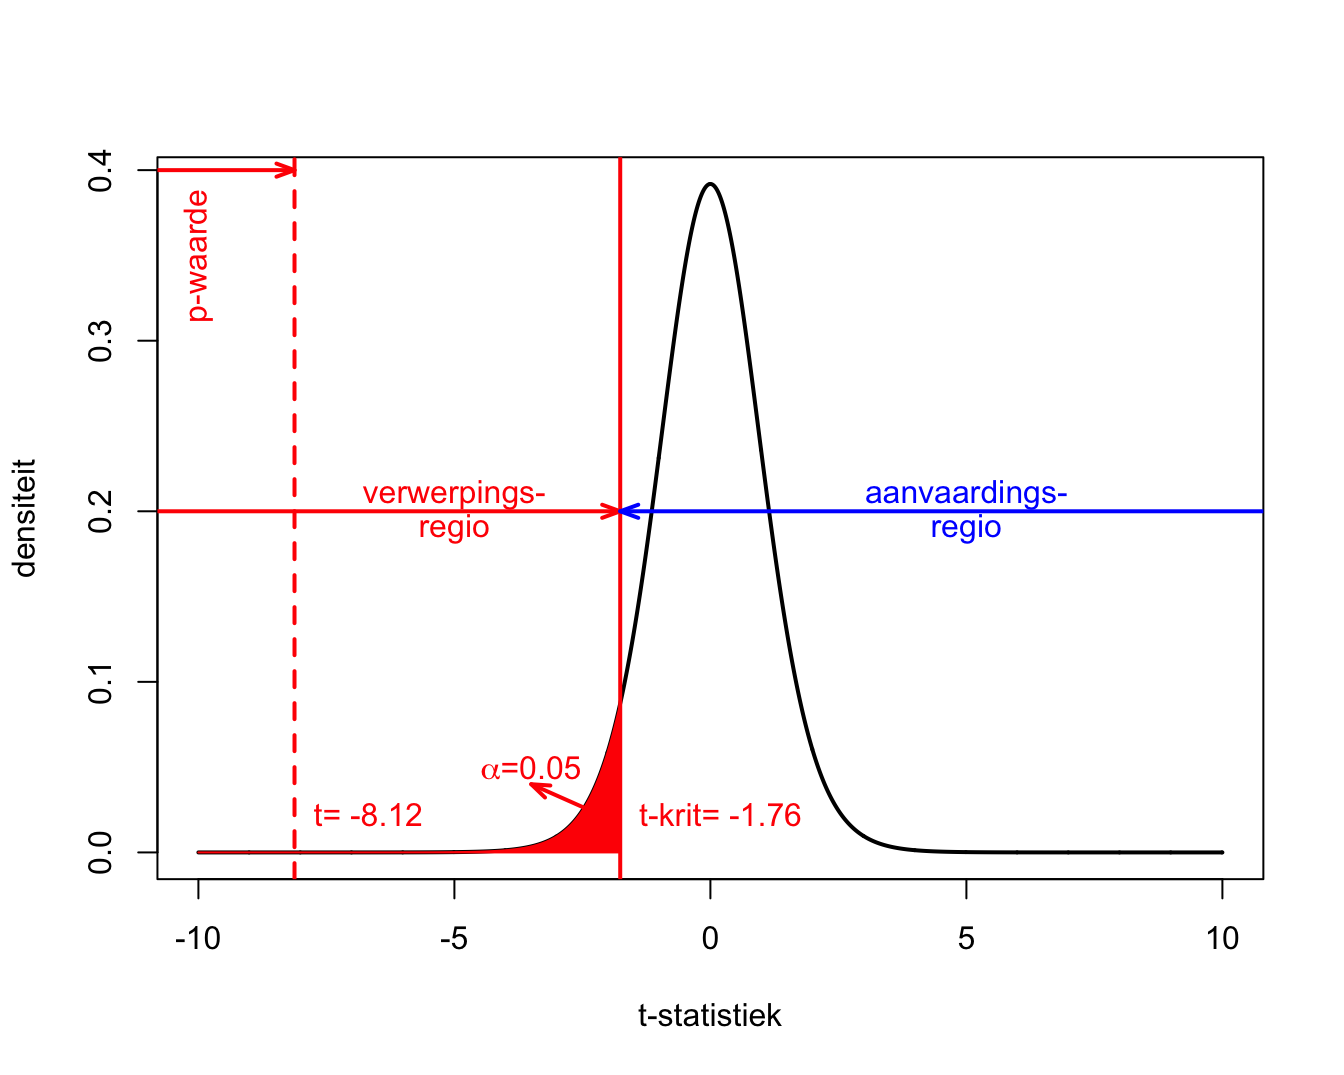
\includegraphics[width=1\linewidth]{Statistiek_2019_2020_files/figure-latex/captoTest-1} 

}

\caption{Interpretatie van p-waarde, kritieke waarde, verwerpingsgebied, aanvaardingsgebied voor het captopril voorbeeld.}\label{fig:captoTest}
\end{figure}

\subsection{Beslissingsfouten}\label{beslissingsfouten}

Aangezien de beslissing over het al dan niet verwerpen van de
nulhypothese bepaald wordt door slechts een steekproef te observeren,
kunnen volgende beslissing genomen worden:

\begin{table}[H]
\centering
\begin{tabular}{c|c|c}
\hline
\multicolumn{1}{c|}{ } & \multicolumn{2}{c}{Werkelijkheid} \\
\cline{2-3}
Besluit & H0 & H1\\
\hline
Aanvaard H0 & OK & Type II (β)\\
\hline
Verwerp H0 & Type I (α) & OK\\
\hline
\end{tabular}
\end{table}

Het schema geeft de vier mogelijke situaties:

\begin{itemize}
\item
  \(H_0\) is in werkelijkheid waar, en dit wordt ook besloten aan de
  hand van de statistische test (dus geen beslissingsfout)
\item
  \(H_1\) is in werkelijkheid waar, en dit wordt ook besloten aan de
  hand van de statistische test (dus geen beslissingsfout)
\item
  \(H_0\) is in werkelijkheid waar, maar aan de hand van de statistische
  test wordt besloten om \(H_0\) te verwerpen en \(H_1\) te concluderen.
  Dus \(H_1\) wordt foutief besloten. Dit is een zogenaamde \textbf{type
  I} fout.
\item
  \(H_1\) is in werkelijkheid waar, maar aan de hand van de statistische
  test wordt besloten om \(H_0\) te aanvaarden. Dit is een zogenaamde
  \textbf{type II} fout. Dus \(H_0\) wordt foutief aanvaard.
\end{itemize}

De beslissing is gebaseerd op een teststatistiek \(T\) die een
toevalsveranderlijke is. De beslissing is dus ook stochastisch en aan de
vier mogelijke situaties uit bovenstaand schema kunnen dus
probabiliteiten toegekend worden. Net zoals voor het afleiden van de
steekproefdistributie van de teststatistiek, moeten we de distributie
van de steekproefobservaties kennen alvorens het stochastisch gedrag van
de beslissingen te kunnen beschrijven. Indien we aannemen dat \(H_0\)
waar is, dan is de distributie van \(T\) gekend en kunnen ook de kansen
op de beslissingen bepaald worden voor de eerste kolom van de tabel.

We starten met de kans op een type I fout (hier uitgewerkt voor het
captopril voor beeld):
\[\text{P}\left[\text{type I fout}\right]=\text{P}\left[\text{verwerp }H_0 \mid H_0\right] = \text{P}_0\left[T<t_{n-1;1-\alpha}\right]=\alpha.\]
Dit geeft ons meteen een interpretatie van het significantieniveau
\(\alpha\): het is de kans op het maken van een type I fout. De
constructie van de statistische test garandeert dus dat de kans op het
maken van een type I fout gecontroleerd wordt op het significantieniveau
\(\alpha\). De kans op het correct aanvaarden van \(H_0\) is dus
\(1-\alpha\). Verder kan aangetoond worden dat de p-waarde onder \(H_0\)
uniform verdeeld is. Het leidt dus tot een uniforme
beslissingsstrategie.

Het bepalen van de kans op een type II fout is minder evident omdat de
alternatieve hypothese minder éénduidig is als de nulhypothese. In het
captopril voorbeeld is \(H_1: \mu<0\); met deze informatie wordt de
distributie van de steekproefobservaties niet volledig gespecifieerd en
dus ook niet de distributie van de teststatistiek. Dit impliceert dat we
eigenlijk de kans op een type II fout niet kunnen berekenen. De
klassieke \emph{work-around} bestaat erin om één specifieke distributie
te kiezen die voldoet aan \(H_1\).

\[H_1(\delta): \mu=0-\delta \text{ voor een }\delta>0.\]

De parameter \(\delta\) kwantificeert de afwijking van de nulhypothese.

De \textbf{kracht} van een test (Engels: \emph{power}) is een kans die
meer frequent gebruikt wordt dan de kans op een type II fout \(\beta\).
De kracht wordt gedefinieerd als

\[\pi(\delta) = 1-\beta(\delta) = \text{P}_\delta\left[T>t_{n-1;1-\alpha}\right]=\text{P}_\delta\left[P<\alpha\right].\]

De kracht van een niveau-\(\alpha\) test voor het detecteren van een
afwijking \(\delta\) van het gemiddelde onder de nulhypothese
\(\mu_0=0\) is dus de kans dat de niveau-\(\alpha\) test dit detecteert
wanneer de afwijking in werkelijkheid \(\delta\) is.

Merk op dat \(\pi(0)=\alpha\) en de kracht van een test toeneemt als de
afwijking van de nulhypothese toeneemt.

De \textbf{kracht} van de test (d.i. de kans om Type II fouten te
vermijden) wordt typisch niet gecontroleerd, tenzij d.m.v. studiedesign
en steekproefgrootte.

\textbf{Interpretatie}

Stel dat we voor een gegeven dataset bekomen dat \(p<\alpha\), m.a.w.
\(H_0\) wordt verworpen. Volgens het schema van de beslissingsfouten
zijn er dan slechts twee mogelijkheden (zie onderste rij van schema):
ofwel is de beslissing correct, ofwel hebben we een type I fout gemaakt.
Over de type I fout weten we echter dat ze slechts voorkomt met een
kleine kans. Anderzijds, indien \(p\geq \alpha\) en we \(H_0\) niet
verwerpen, dan zijn er ook twee mogelijkheden: ofwel is de beslissing
correct, ofwel hebben we een type II fout gemaakt. De kans op een type
II fout (\(\beta\)) is echter niet gecontroleerd op een gespecifieerde
waarde. De statistische test is zodanig geconstrueerd dat ze enkel de
kans op een type I fout controleert (op \(\alpha\)). Om wetenschappelijk
eerlijk te zijn, moeten we een pessimistische houding aannemen en er
rekening mee houden dat \(\beta\) groot zou kunnen zijn (i.e.~een kleine
kracht).

Bij \(p < \alpha\) wordt de nulhypothese verworpen en we mogen hieruit
concluderen dat \(H_1\) waarschijnlijk juist is. Dit noemen we een
sterke conclusie. Bij \(p\geq \alpha\) wordt de nulhypothese aanvaard,
maar dat impliceert niet dat we concluderen dat \(H_0\) juist is. We
kunnen enkel besluiten dat de data onvoldoende bewijskracht tegen
\(H_0\) ten gunste van \(H_1\) bevatten. Dit noemen we een daarom zwakke
conclusie.

\subsection{Conclusies Captopril
voorbeeld.}\label{conclusies-captopril-voorbeeld.}

De test die we hebben uitgevoerd is in de literatuur ook bekend als de
\textbf{one sample t-test} op het verschil of als een \textbf{gepaarde
t-test}, we beschikken immers over gepaarde gegevens per patiënt. De
test is eenzijdig uitgevoerd. We testen tegen het alternatief dat er een
bloeddrukdaling is.

Beide testen (one sample t-test op het verschil en de gepaarde t-test)
geven ons inderdaad dezelfde resultaten:

\begin{Shaded}
\begin{Highlighting}[]
\KeywordTok{t.test}\NormalTok{(delta, }\DataTypeTok{alternative =} \StringTok{"less"}\NormalTok{)}
\end{Highlighting}
\end{Shaded}

\begin{verbatim}
## 
##  One Sample t-test
## 
## data:  delta
## t = -8.1228, df = 14, p-value = 5.732e-07
## alternative hypothesis: true mean is less than 0
## 95 percent confidence interval:
##       -Inf -14.82793
## sample estimates:
## mean of x 
## -18.93333
\end{verbatim}

\begin{Shaded}
\begin{Highlighting}[]
\KeywordTok{with}\NormalTok{(captopril, }\KeywordTok{t.test}\NormalTok{(SBPa, SBPb, }\DataTypeTok{paired =} \OtherTok{TRUE}\NormalTok{, }\DataTypeTok{alternative =} \StringTok{"less"}\NormalTok{))}
\end{Highlighting}
\end{Shaded}

\begin{verbatim}
## 
##  Paired t-test
## 
## data:  SBPa and SBPb
## t = -8.1228, df = 14, p-value = 5.732e-07
## alternative hypothesis: true difference in means is less than 0
## 95 percent confidence interval:
##       -Inf -14.82793
## sample estimates:
## mean of the differences 
##               -18.93333
\end{verbatim}

We kunnen op basis van de test het volgende concluderen: Na toediening
van captopril is er een extreem significante verlaging van de
systolische bloeddruk bij patiënten met hypertensie (\(p << 0.001\)). De
systolische bloeddruk neemt gemiddeld met 18.9 mm kwik af na de
behandeling met captopril (95\% BI {[}\(-\infty,-14.82\){]} mm Hg).

Merk op dat we

\begin{enumerate}
\def\labelenumi{\arabic{enumi}.}
\tightlist
\item
  Een eenzijdig interval rapporteren gezien we enkel geïnteresseerd zijn
  om aan te tonen dat er een bloeddrukdaling is.
\item
  Door het pre-test/post-test design geen uitsluitsel kunnen geven of
  dit te wijten is aan de werking van het middel of aan een placebo
  effect. Er was geen goeie controle! Het gebrek van een goeie controle
  is veelal een probleem bij pre-test/post-test designs.
\end{enumerate}

\subsection{Eenzijdig of tweezijdig
toetsen?}\label{eenzijdig-of-tweezijdig-toetsen}

De test in het captopril voorbeeld was een eenzijdige test. We wensen
immers enkel te detecteren of de captopril behandeling de bloeddruk
gemiddeld gezien doet dalen.

In andere gevallen of een andere context wenst men enkel een stijging te
detecteren.\\
Stel dat men het bloeddrukverschil had gedefineerd als
\(X_{i}^\prime=Y_{i}^\text{voor}-Y_{i}^\text{na}\) dan zouden positieve
waarden aangeven dat er een bloeddrukdaling was na de behandeling van
captopril: de bloeddruk bij aanvang is dan immers groter dan na de
behandeling. De gemiddelde bloeddrukverandering in de populatie noteren
we nu als \(\mu^\prime=\text{E}[X^*]\). In dat geval hadden we een
eenzijdige test uit moeten voeren om \(H_0: \mu^\prime=0\) te testen
tegen \(H_1: \mu^\prime>0\). Voor deze test kunnen we de p-waarde als
volgt berekenen: \[p=\text{P}_0\left[T\geq t\right].\]

We voeren nu de analyse uit in R op basis van de toevallige
veranderlijke \(X^\prime\). We zullen nu het argument
\texttt{alternative="greater"} gebruiken in de \texttt{t.test} functie
zodat we de nulhypothese toetsen tegen het alternatief
\(H_1: \mu^\prime>0\):

\begin{Shaded}
\begin{Highlighting}[]
\NormalTok{delta2 <-}\StringTok{ }\NormalTok{captopril}\OperatorTok{$}\NormalTok{SBPb }\OperatorTok{-}\StringTok{ }\NormalTok{captopril}\OperatorTok{$}\NormalTok{SBPa}
\KeywordTok{t.test}\NormalTok{(delta2, }\DataTypeTok{alternative =} \StringTok{"greater"}\NormalTok{)}
\end{Highlighting}
\end{Shaded}

\begin{verbatim}
## 
##  One Sample t-test
## 
## data:  delta2
## t = 8.1228, df = 14, p-value = 5.732e-07
## alternative hypothesis: true mean is greater than 0
## 95 percent confidence interval:
##  14.82793      Inf
## sample estimates:
## mean of x 
##  18.93333
\end{verbatim}

Uiteraard bekomen we met deze analyse exact dezelfde p-waarde en
hetzelfde betrouwbaarheidsinterval. Enkel het teken is omgewisseld.

Naast eenzijdige testen kunnen eveneens tweezijdige testen worden
uitgevoerd. Het had gekund dat de onderzoekers de werking van het nieuwe
medicijn captopril wensten te testen, maar het werkingsmechanisme nog
niet kenden in de ontwerpfase. In dat geval zou het eveneens interessant
geweest zijn om zowel een stijging als een daling van de bloeddruk te
kunnen detecteren. Hiervoor zou men een tweezijdige toetsstrategie
moeten gebruiken waarbij men de nulhypothese \[H_0: \mu=0\] gaat testen
versus het alternatieve hypothese \[H_1: \mu\neq0,\] zodat het
gemiddelde onder de alternatieve hypothese verschillend is van 0. Het
kan zowel een positieve of negatieve afwijking zijn en men weet niet bij
aanvang van de studie in welke richting het werkelijk gemiddelde zal
afwijken onder de alternatieve hypothese.

We kunnen tweezijdig testen op het \(\alpha=5\%\) significantieniveau
door

\begin{enumerate}
\def\labelenumi{\arabic{enumi}.}
\tightlist
\item
  een kritieke waarde af te leiden:

  \begin{itemize}
  \tightlist
  \item
    Bij een tweezijdige test kan het effect onder de alternatieve
    hypothese zowel positief of negatief zijn. Hierdoor zullen we onder
    de nulhypothese de kans berekenen om onder de nulhypothese een
    effect te observeren dat meer extreem is dan het resultaat dat werd
    geobserveerd in de steekproef. In deze context betekent ``meer
    extreem'' dat de statistiek groter is in absolute waarde dan het
    geobserveerde resultaat, want zowel grote (sterk positieve) als
    kleine (sterk negatieve) waarden zijn een indicatie van een
    afwijking van de nulhypothese.
  \item
    Om een kritieke waarde af te leiden,zullen we het
    significatie-niveau \(\alpha\) daarom verdelen over de linker en
    rechter staart van de verdeling onder \(H_0\). Gezien de t-verdeling
    symmetrisch is, volgt dat we een kritieke waarde \(c\) kiezen zodat
    er een kans is van \(\alpha/2=2.5\%\) dat \(T\geq c\) en er
    \(\alpha/2=2.5\%\) kans is dat \(T\leq -c\). We kunnen dit ook nog
    als volgt formuleren: Er is onder \(H_0\) \(\alpha=5\%\) kans dat
    \(\vert T\vert\geq c\) (zie Figuur \ref{fig:captoTest2}).
  \end{itemize}
\item
  We kunnen ook gebruik maken van een tweezijdige p-waarde:

  \begin{eqnarray*}
    p&=&\text{P}_0\left[T\leq -|t|\right] + \text{P}_0\left[T\geq |t|\right]\\
    &=&\text{P}_0\left[\vert T\vert \geq \vert t \vert\right]\\
    &=&\text{P}_0\left[T \geq \vert t \vert\right]\times 2.
    \end{eqnarray*}
\end{enumerate}

We berekenen dus de kans dat de t-statistiek onder \(H_0\) meer extreem
is dan de geobserveerde teststatistiek \(t\) in de steekproef. Waarbij
meer extreem tweezijdig moet geïnterpreteerd worden. De teststatistiek
onder \(H_0\) is meer extreem als hij groter is in absolute waarde dan
\(\vert t \vert\), de geobserveerde test statistiek. Gezien de verdeling
symmetrisch is, kunnen we ook eerst de kans in de rechter staart van de
verdeling berekenen en deze kans vervolgens vermenigvuldigen met 2
zodoende een tweezijdige p-waarde te bekomen.

Als de onderzoekers niet vooraf gedefineerd hadden dat ze enkel een
bloeddrukdaling wensten te detecteren, dan hadden ze dus een
twee-zijdige test uitgevoerd. Merk op dat het argument
\texttt{alternative} van de \texttt{t.test} functie een default waarde
heeft \texttt{alternative="two.sided"} zodat er standaard tweezijdig
wordt getoetst.

\begin{Shaded}
\begin{Highlighting}[]
\KeywordTok{t.test}\NormalTok{(delta)}
\end{Highlighting}
\end{Shaded}

\begin{verbatim}
## 
##  One Sample t-test
## 
## data:  delta
## t = -8.1228, df = 14, p-value = 1.146e-06
## alternative hypothesis: true mean is not equal to 0
## 95 percent confidence interval:
##  -23.93258 -13.93409
## sample estimates:
## mean of x 
## -18.93333
\end{verbatim}

We bekomen nog steeds een exteem significant resultaat. De p-waarde is
echter dubbel zo groot omdat we tweezijdig testen. We verkrijgen
eveneens een tweezijdig betrouwbaarheidsinterval. De tweezijdige
toetsstrategie wordt weergegeven in Figuur \ref{fig:captoTest2}.

\begin{figure}

{\centering 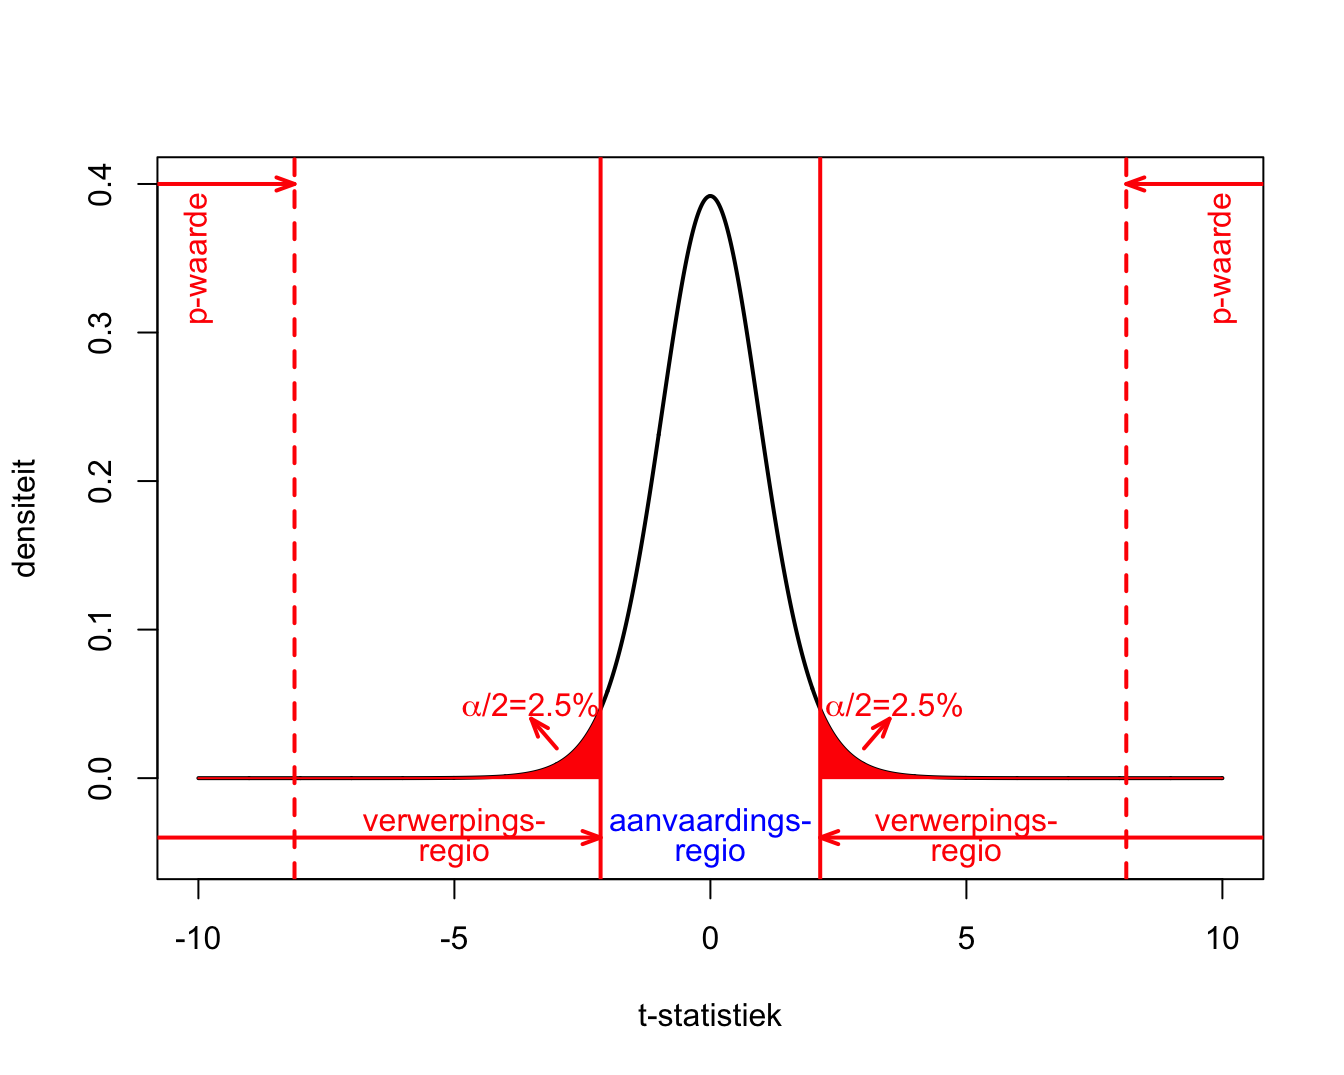
\includegraphics[width=1\linewidth]{Statistiek_2019_2020_files/figure-latex/captoTest2-1} 

}

\caption{Interpretatie van p-waarde, kritieke waarde, verwerpingsgebied, aanvaardingsgebied voor het captopril voorbeeld wanneer we een tweezijdige toets uitvoeren.}\label{fig:captoTest2}
\end{figure}

We kunnen ons nu de vraag stellen wanneer we eenzijdig of tweezijdig
toetsen. Met een eenzijdige toets kan men gemakkelijker een alternatieve
hypothese aantonen (op voorwaarde dat ze waar is) dan met een
tweezijdige toets. Dit komt essentieel omdat bij zo'n toets alle
informatie kan worden aangewend om in 1 enkele richting te zoeken.
Precies daarom vergt de eenzijdige toets een extra beschouwing vóór de
aanvang van de studie. Ook al hebben we sterke a priori vermoedens, vaak
kunnen we niet zeker zijn dat dat zo is. Anders was er immers geen reden
om dit te willen toetsen.

Als men een eenzijdige test voorstelt, maar men vindt een resultaat in
de andere richting dat formeel statistisch significant is, dan is het
niet geschikt om dit te zien als bewijs voor een werkelijk effect in die
richting. Dat is omdat de onderzoekers die mogelijkheid uitgesloten
hebben bij de planning van de studie en het resultaat daarom zó
onverwacht is dat het als een vals positief resultaat kan gezien worden.
Een eenzijdige test is om die reden niet aanbevolen. Een tweezijdige
toets is altijd verdedigbaar omdat ze in principe toelaat om elke
afwijking van de nulhypothese te detecteren. Ze worden daarom het meest
gebruikt en ten zeerste aangeraden. Het is \textbf{nooit toegelaten} om
een tweezijdige toets in een eenzijdige toets om te zetten \textbf{op
basis van wat men observeert in de gegevens}! Anders wordt de type I
fout van de toetsingsstrategie niet correct gecontroleerd.

Dat wordt geïllustreerd in de onderstaande simulatie. We evalueren twee
strategieën, de correcte tweezijdige test en een test waar we eenzijdig
toetsen op basis van het teken van het geobserveerde effect.

\begin{Shaded}
\begin{Highlighting}[]
\KeywordTok{set.seed}\NormalTok{(}\DecValTok{115}\NormalTok{)}
\NormalTok{mu <-}\StringTok{ }\DecValTok{0}
\NormalTok{sigma <-}\StringTok{ }\DecValTok{9}
\NormalTok{nSim <-}\StringTok{ }\DecValTok{1000}
\NormalTok{alpha <-}\StringTok{ }\FloatTok{0.05}
\NormalTok{n <-}\StringTok{ }\DecValTok{15}
\NormalTok{pvalsCor <-}\StringTok{ }\NormalTok{pvalsInCor <-}\StringTok{ }\KeywordTok{array}\NormalTok{(}\DecValTok{0}\NormalTok{, nSim)}
\ControlFlowTok{for}\NormalTok{ (i }\ControlFlowTok{in} \DecValTok{1}\OperatorTok{:}\NormalTok{nSim) \{}
\NormalTok{    x <-}\StringTok{ }\KeywordTok{rnorm}\NormalTok{(n, }\DataTypeTok{mean =}\NormalTok{ mu, }\DataTypeTok{sd =}\NormalTok{ sigma)}
\NormalTok{    pvalsCor[i] <-}\StringTok{ }\KeywordTok{t.test}\NormalTok{(x)}\OperatorTok{$}\NormalTok{p.value}
    \ControlFlowTok{if}\NormalTok{ (}\KeywordTok{mean}\NormalTok{(x) }\OperatorTok{<}\StringTok{ }\DecValTok{0}\NormalTok{) }
\NormalTok{        pvalsInCor[i] <-}\StringTok{ }\KeywordTok{t.test}\NormalTok{(x, }\DataTypeTok{alternative =} \StringTok{"less"}\NormalTok{)}\OperatorTok{$}\NormalTok{p.value }\ControlFlowTok{else}\NormalTok{ pvalsInCor[i] <-}\StringTok{ }\KeywordTok{t.test}\NormalTok{(x, }\DataTypeTok{alternative =} \StringTok{"greater"}\NormalTok{)}\OperatorTok{$}\NormalTok{p.value}
\NormalTok{\}}
\KeywordTok{mean}\NormalTok{(pvalsCor }\OperatorTok{<}\StringTok{ }\FloatTok{0.05}\NormalTok{)}
\end{Highlighting}
\end{Shaded}

\begin{verbatim}
## [1] 0.049
\end{verbatim}

\begin{Shaded}
\begin{Highlighting}[]
\KeywordTok{mean}\NormalTok{(pvalsInCor }\OperatorTok{<}\StringTok{ }\FloatTok{0.05}\NormalTok{)}
\end{Highlighting}
\end{Shaded}

\begin{verbatim}
## [1] 0.106
\end{verbatim}

We zien inderdaad dat de type I fout correct gecontroleerd wordt op het
nominaal significantie-niveau \(\alpha\) wanneer we tweezijdig testen en
dat dit helemaal niet het geval is wanneer we eenzijdige toetsen op
basis van het teken van het geobserveerde effect.

\section{Two-sample t-test}\label{two-sample-t-test}

Een two-sample t-test is een statistische toets die werd ontwikkeld om
verschillen in gemiddelde te detecteren tussen twee onafhankelijke
groepen. We introduceren eerst een motiverende dataset. Men vermoedt dat
hinderlijke geur onder de oksels (bromhidrosis) wordt veroorzaakt door
specifieke microorganismen die behoren tot de groep van de
\emph{Corynebacterium spp.}. Het is immers niet het zweet dat de geur
veroorzaakt, maar de geur is het resultaat van specifieke bacteriën die
het zweet metaboliseren. Een andere sterk abundante groep wordt gevormd
door de \emph{Staphylococcus spp.}. In de CMET onderzoeksgroep van de
Universiteit Gent wordt onderzoek verricht naar de mogelijkheid van
microbiële transplanties in de oksels om mensen van de hinderlijke
okselgeur te verlossen. Deze therapie bestaat erin om eerst het
oksel-microbioom te verwijderen door een lokale antibiotica behandeling,
en vervolgens via een microbiële transplantie de populatie te
beïnvloeden. (zie: \url{https://youtu.be/9RIFyqLXdVw} )

De primaire onderzoeksvraag: leidt de microbiële transplantatie na zes
weken tot een verandering in de relatieve abundantie van
\emph{Staphylococcus spp.} in het oksel microbioom in vergelijking met
een placebo behandeling die enkel bestaat uit een antibiotica
behandeling? Twintig personen met een hinderlijke okselgeur worden
willekeurig toegekend aan twee behandelingsgroepen: placebo (enkel
antibiotica) en transplantie (antibiotica, gevolgd door microbiële
transplantatie). Zes weken na de start van de behandeling wordt een
staal van de huid uit de okselholte genomen en worden de relatieve
abundanties van \emph{Staphylococcus spp.} en \emph{Corynebacterium
spp.} in het microbioom gemeten via DGGE (\emph{Denaturing Gradient Gel
Electrophoresis}).

De dataset bevat de variabelen Staph en Cor die de relatieve abundanties
(\%) weergeven van \emph{Staphylococcus spp.} en \emph{Corynebacterium
spp.} De variabele Rel werd berekend als \[
    \text{Rel}=\frac{\text{Staph}}{\text{Staph}+\text{Cor}}.
  \] Deze variabele is het relatief aandeel van \emph{Staphylococcus
spp.} op het totaal aantal \emph{Staphylococcus spp.} en
\emph{Corynebacterium spp.}.

In de folder dataset staat de file \texttt{oksel.rda}, een dump van het
R object \texttt{oksel}, een data frame voor het oksel voorbeeld. R
objecten die zijn opgeslagen kunnen via de \texttt{load(.)} functie
worden ingelezen. De resultaten worden weergegeven in Figuur
\ref{fig:okselBox}.

\begin{Shaded}
\begin{Highlighting}[]
\KeywordTok{load}\NormalTok{(}\StringTok{"dataset/oksel.rda"}\NormalTok{)}
\KeywordTok{head}\NormalTok{(oksel)}
\end{Highlighting}
\end{Shaded}

\begin{verbatim}
##              trt Staph  Cor      Rel
## 1 trt 2: placebo  34.7 28.4 54.99208
## 2 trt 2: placebo  16.4 35.1 31.84466
## 3 trt 2: placebo  31.4 45.0 41.09948
## 4 trt 2: placebo  44.7 30.4 59.52064
## 5 trt 2: placebo  45.9 26.3 63.57341
## 6 trt 2: placebo  30.7 43.3 41.48649
\end{verbatim}

\begin{Shaded}
\begin{Highlighting}[]
\CommentTok{# outline = FALSE, geen outliers alle datapunten}
\CommentTok{# worden toegevoegd via stripchart dus ook outliers}
\CommentTok{# zijn zichtbaar}
\KeywordTok{boxplot}\NormalTok{(Rel }\OperatorTok{~}\StringTok{ }\NormalTok{trt, }\DataTypeTok{data =}\NormalTok{ oksel, }\DataTypeTok{xlab =} \StringTok{"behandeling"}\NormalTok{, }
    \DataTypeTok{ylab =} \StringTok{"Relatieve abundantie"}\NormalTok{, }\DataTypeTok{outline =} \OtherTok{FALSE}\NormalTok{)}
\KeywordTok{set.seed}\NormalTok{(}\DecValTok{394}\NormalTok{)}
\KeywordTok{stripchart}\NormalTok{(Rel }\OperatorTok{~}\StringTok{ }\NormalTok{trt, }\DataTypeTok{data =}\NormalTok{ oksel, }\DataTypeTok{vertical =} \OtherTok{TRUE}\NormalTok{, }
    \DataTypeTok{method =} \StringTok{"jitter"}\NormalTok{, }\DataTypeTok{pch =} \DecValTok{19}\NormalTok{, }\DataTypeTok{col =} \KeywordTok{c}\NormalTok{(}\StringTok{"bisque"}\NormalTok{, }
        \StringTok{"coral"}\NormalTok{), }\DataTypeTok{add =} \OtherTok{TRUE}\NormalTok{)}
\KeywordTok{set.seed}\NormalTok{(}\DecValTok{394}\NormalTok{)}
\KeywordTok{stripchart}\NormalTok{(Rel }\OperatorTok{~}\StringTok{ }\NormalTok{trt, }\DataTypeTok{data =}\NormalTok{ oksel, }\DataTypeTok{vertical =} \OtherTok{TRUE}\NormalTok{, }
    \DataTypeTok{method =} \StringTok{"jitter"}\NormalTok{, }\DataTypeTok{pch =} \DecValTok{1}\NormalTok{, }\DataTypeTok{add =} \OtherTok{TRUE}\NormalTok{)}
\end{Highlighting}
\end{Shaded}

\begin{figure}

{\centering 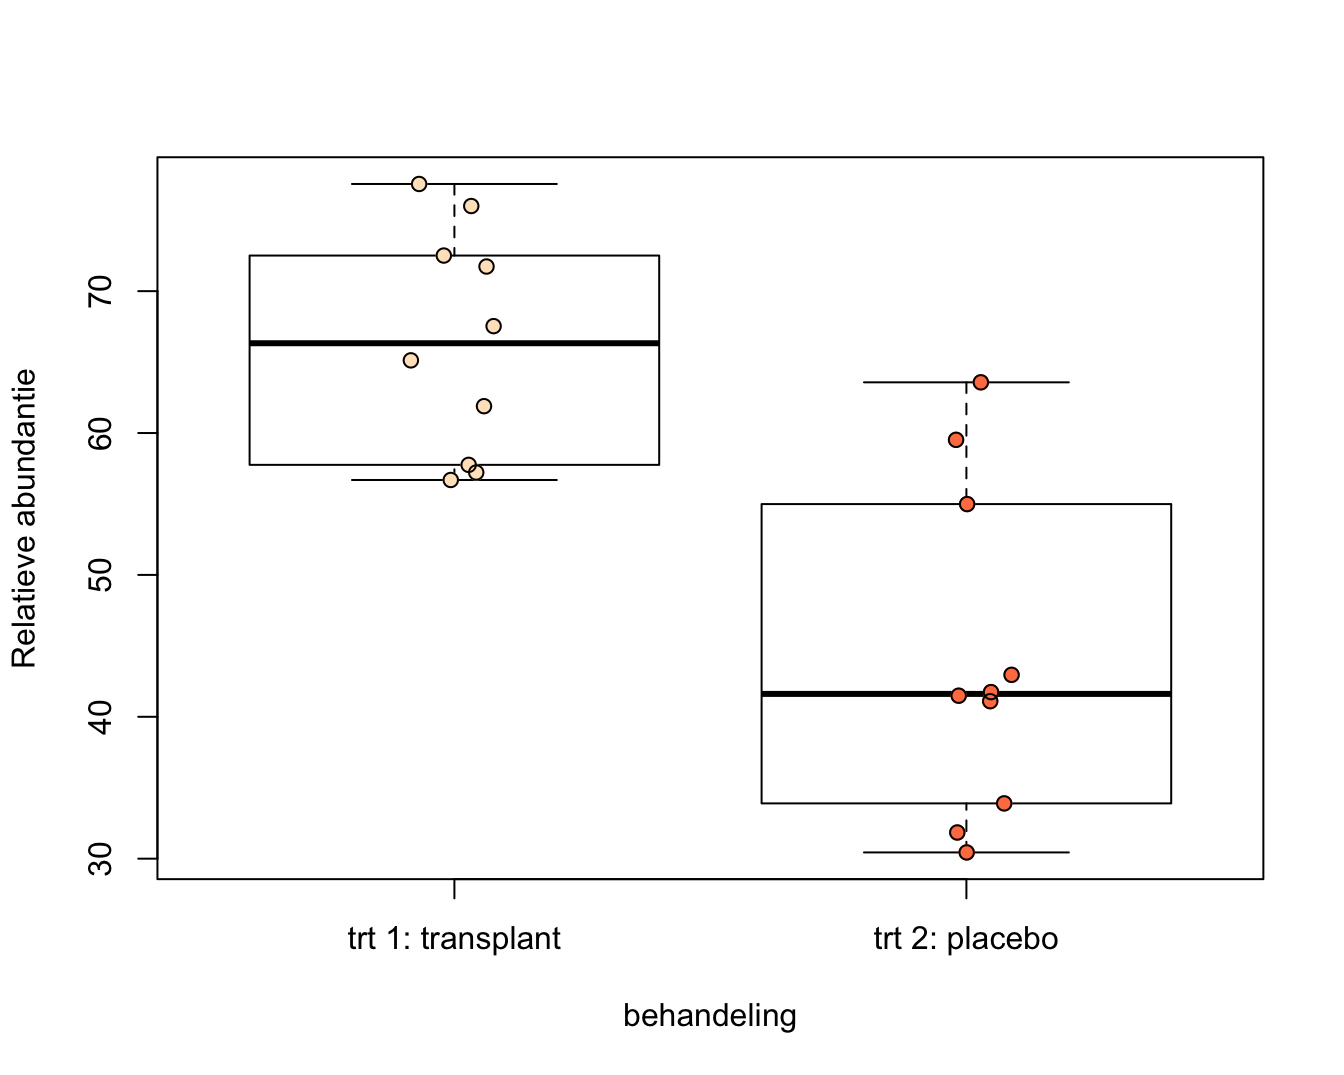
\includegraphics[width=1\linewidth]{Statistiek_2019_2020_files/figure-latex/okselBox-1} 

}

\caption{Boxplot van de relatieve Staphylococcus spp. abundantie t.o.v. het totaal van Staphylococcus spp. en Corynebacterium spp., voor beide behandelingsgroepen.}\label{fig:okselBox}
\end{figure}

\begin{Shaded}
\begin{Highlighting}[]
\KeywordTok{par}\NormalTok{(}\DataTypeTok{mfrow =} \KeywordTok{c}\NormalTok{(}\DecValTok{1}\NormalTok{, }\DecValTok{2}\NormalTok{))}
\NormalTok{oksel}\OperatorTok{$}\NormalTok{trt =}\StringTok{ }\KeywordTok{as.factor}\NormalTok{(oksel}\OperatorTok{$}\NormalTok{trt)  }\CommentTok{#zet charactervector om in factor}
\ControlFlowTok{for}\NormalTok{ (i }\ControlFlowTok{in} \KeywordTok{levels}\NormalTok{(oksel}\OperatorTok{$}\NormalTok{trt)) }\KeywordTok{with}\NormalTok{(}\KeywordTok{subset}\NormalTok{(oksel, trt }\OperatorTok{==}\StringTok{ }
\StringTok{    }\NormalTok{i), \{}
    \KeywordTok{qqPlot}\NormalTok{(Rel, }\DataTypeTok{main =}\NormalTok{ i)}
\NormalTok{\})}
\end{Highlighting}
\end{Shaded}

\begin{figure}

{\centering 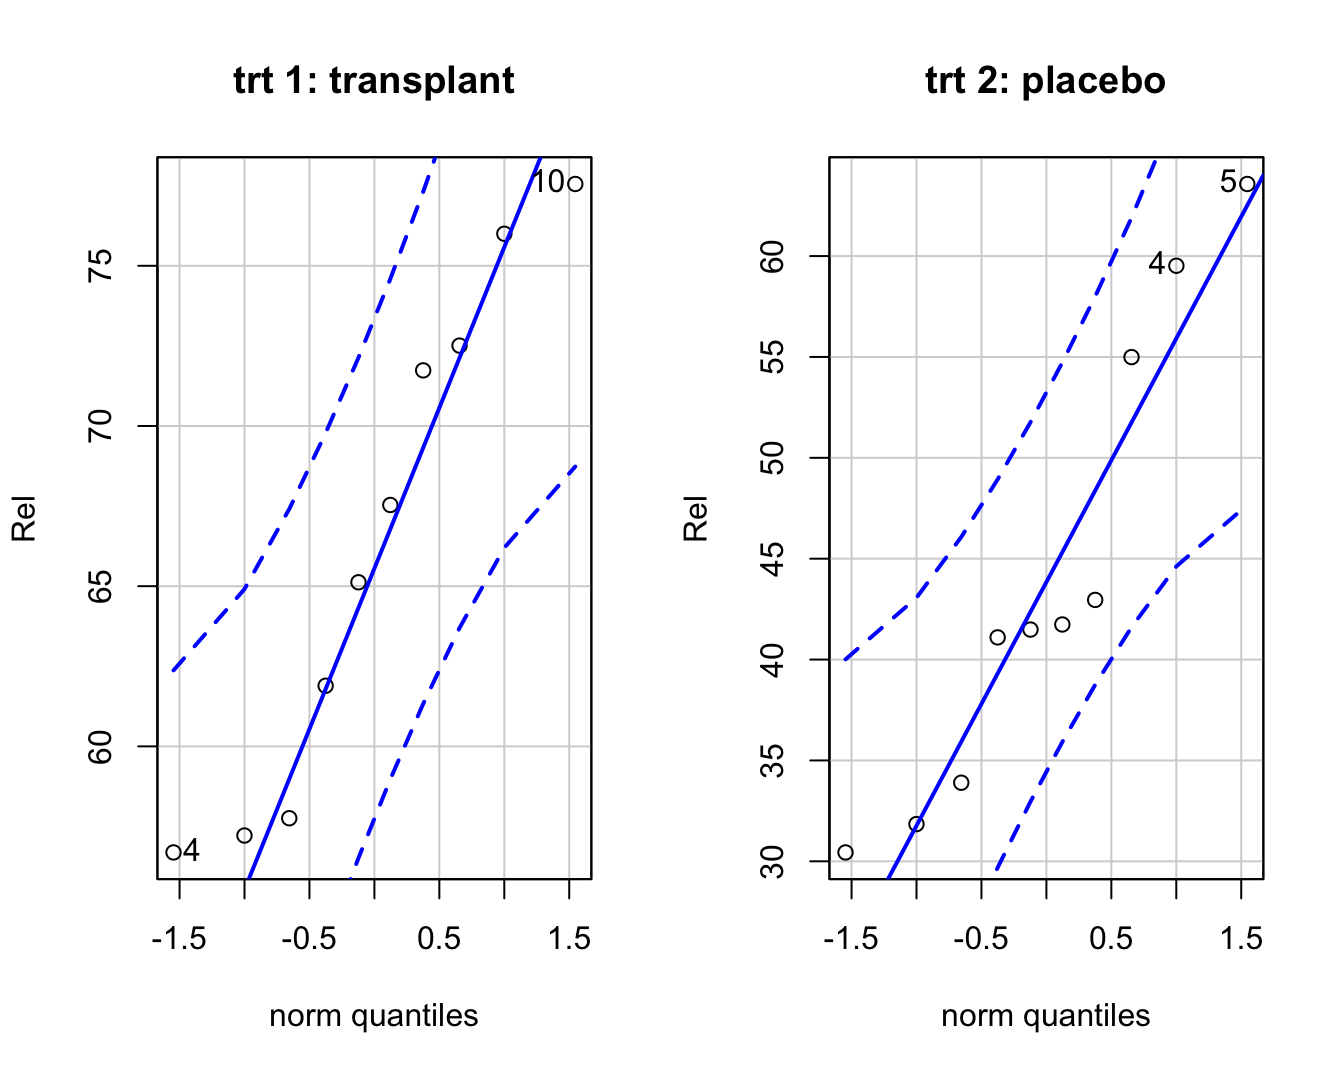
\includegraphics[width=1\linewidth]{Statistiek_2019_2020_files/figure-latex/okselQQ-1} 

}

\caption{QQ-plots van relatieve Staphylococcus spp. abundantie t.o.v. het totaal van Staphylococcus spp. en Corynebacterium spp.}\label{fig:okselQQ}
\end{figure}

Normaliteit van de data in beide groepen wordt ook nagegaan d.m.v.
QQ-plots (zie Figuur \ref{fig:okselQQ}). De QQ-plots geven geen te grote
afwijkingen weer van normaliteit.

We introduceren eerst de notatie. Stel \(Y_{ij}\) de uitkomst van
observatie \(i=1,\ldots, n_j\) uit populatie \(j=1,2\). We zullen
dikwijls de term \textbf{behandeling} of \textbf{groep} gebruiken in
plaats van populatie, zelfs wanneer de twee populaties niet
geïnterpreteerd kunnen worden als behandelingen. Beschouw het als een
(misgroeide) conventie. In de context van het voorbeeld is behandeling
\(j=1\) de microbiële transplantatie en behandeling \(j=2\) de placebo
behandeling.

We veronderstellen

\[Y_{ij}\text{ i.i.d. } N(\mu_j,\sigma^2)\;\;\;i=1,\ldots,n_i\;j=1,2.\]

Merk op dat dit inhoudt dat gelijke varianties verondersteld worden. De
eigenschap van gelijke varianties wordt ook aangeduid met de term
\textbf{homoskedasticiteit}, en ongelijke varianties met
\textbf{heteroskedasticiteit}.

We zijn geïnteresseerd in het testen van de nulhypothese
\[ H_0: \mu_1 = \mu_2 \] tegenover de alternatieve hypothese
\[  H_1: \mu_1 \neq \mu_2 .\] De alternatieve hypothese drukt dus de
onderzoeksvraag uit: een verschil in relatieve abundantie van
\emph{Staphylococcus spp.} na microbiële transplantatie t.o.v. de
placebo behandeling.\\
De nul en alternatieve hypothese kunnen ook worden uitgedrukt in termen
van de effectgrootte tussen behandeling en placebo groep
\(\mu_1-\mu_2\): \[H_0: \mu_1-\mu_2 = 0,\] \[H_1: \mu_1-\mu_2 \neq 0.\]

We kunnen de effectgrootte in het experiment schatten a.d.h.v. de
steekproefgemiddeldes: \[\hat \mu_1-\hat \mu_2=\bar Y_1 -\bar Y_2.\]
Gezien de experimentele eenheden onafhankelijk zijn, zijn de
steekproefgemiddeldes dat ook en is de variantie op het verschil:
\[\text{Var}_{\bar Y_1 -\bar Y_2}=\frac{\sigma^2}{n_1}+\frac{\sigma^2}{n_2}=\sigma^2 \left(\frac{1}{n_1}+\frac{1}{n_2}\right).\]
De standard error is bijgevolg:
\[\sigma_{\bar Y_1 -\bar Y_2}=\sigma\sqrt{\frac{1}{n_1}+\frac{1}{n_2}}.\]

We zouden de variantie apart kunnen schatten in elke groep aan de hand
van de steekproefvariatie, maar als we gelijkheid van variantie kunnen
veronderstellen kan de variantie meer precies worden geschat door
gebruik te maken van alle gegevens in beide groepen. Deze
variatieschatter wordt ook de gepoolde variantieschatter genoemd:
\(S^2_p\).

Op basis van de observaties uit de eerste groep kan \(\sigma^2_1\)
geschat worden als
\[S_1^2 = \frac{1}{n_1-1}\sum_{i=1}^{n_1} (Y_{i1}-\bar{Y}_1)^2.\]

Analoog: op basis van de observaties uit de tweede groep kan
\(\sigma^2_2\) geschat worden als
\[S_2^2 = \frac{1}{n_2-1}\sum_{i=1}^{n_2} (Y_{i2}-\bar{Y}_2)^2.\]

Merk op dat we homoscedasticiteit veronderstellen,
\(\sigma_1^2=\sigma_2^2=\sigma^2\). Dus \(S_1^2\) en \(S_2^2\) zijn
schatters zijn voor dezelfde parameter \(\sigma^2\). Daarom kunnen ze
gezamenlijk gebruikt worden om tot één schatter te komen die alle
\(n_1+n_2\) observaties gebruikt:
\[  S_p^2 = \frac{n_1-1}{n_1+n_2-2} S_1^2 + \frac{n_2-1}{n_1+n_2-2} S_2^2 = \frac{1}{n_1+n_2-2}\sum_{j=1}^2\sum_{i=1}^{n_j} (Y_{ij} - \bar{Y}_j)^2.\]

De gepoolde variantieschatter wordt dus geschat door gebruik te maken
van de kwadratische afwijkingen tussen de observaties en hun
groepsgemiddelde en dat te delen door het aantal vrijheidsgraden
\(n_1+n_2-2\)\footnote{We hebben \(n_1+n_2\) observaties
  (vrijheidsgraden) in het experiment, om de gepoolde variantie te
  schatten hebben we echter 2 vrijheidsgraden verloren aangezien we
  eerst het gemiddelde in elke groep dienden te bepalen om de variantie
  te kunnen schatten.}.

Nu we de effectgrootte en de standard error op de effectgrootte hebben
kunnen schatten, kunnen we opnieuw een t-statistiek definiëren
(two-sample \(t\)-teststatistiek):

\[T = \frac{\bar{Y}_1-\bar{Y}_2}{\sqrt{\frac{S_p^2}{n_1}+\frac{S_p^2}{n_2}}} = 
  \frac{\bar{Y}_1 - \bar{Y}_2}{S_p\sqrt{\frac{1}{n_1}+\frac{1}{n_2}}}.\]

Als de data onafhankelijk zijn, de steekproefgemiddelden normaal
verdeeld zijn en de variantie in beide groepen gelijk zijn, dan kan men
aantonen de teststatistiek T opnieuw een t-verdeling volgt met
\(n_1+n_2-2\) vrijheidsgraden onder de nulhypothese.

Aangezien de alternatieve hypothese \(H_1: \mu_1 \neq \mu_2\) impliceert
dat de probabiliteitsmassa van de distributie van \(T\) onder \(H_1\)
verschuift naar hogere of lagere waarden, zullen we \(H_0\) wensen te
verwerpen ten gunste van \(H_1\) voor grote absolute waarde van de
teststatistiek. De \(p\)-waarde wordt dus

\begin{eqnarray*}
  p&=&\text{P}_0\left[T\leq -|t|\right] + \text{P}_0\left[T\geq |t|\right]\\
  &=&\text{P}_0\left[\vert T\vert \geq \vert t \vert\right]\\
  &=&\text{P}_0\left[T \geq \vert t \vert\right]\times 2\\
  &=& 2\times(1-F_T(\vert t\vert;n_1+n_2-2)),
  \end{eqnarray*}

met \(F_T(\cdot;n_1+n_2-2)\) de cumulatieve distributiefunctie van
\(t_{n_1+n_2-2}\).

\subsection{Oksel-voorbeeld}\label{oksel-voorbeeld}

De onderzoeksvraag van het oksels-voorbeeld kan vertaald worden in een
nulhypothese en een alternatieve hypothese.

De nulhypothese verwoordt de stelling dat de behandeling geen effect
heeft op de gemiddelde relatieve abundantie van \emph{Staphylococcus
spp.}.

Indien \(\mu_1\) en \(\mu_2\) de gemiddelde abundanties voorstellen in
respectievelijk de transplantatie groep en de placebo groep, dan
schrijven we \[   H_0: \mu_1=\mu_2.\] De alternatieve hypothese
correspondeert met wat we wensen te bewijzen aan de hand van de
experimentele data: een verschil in gemiddelde abundantie van
\emph{Staphylococcus spp.} in de transplantatie groep i.v.m. de placebo
groep. Dus \[H_1: \mu_1\neq \mu_2.\]

De berekeningen kunnen als volgt in R worden uitgevoerd:

\begin{Shaded}
\begin{Highlighting}[]
\NormalTok{ybar1 <-}\StringTok{ }\KeywordTok{mean}\NormalTok{(oksel}\OperatorTok{$}\NormalTok{Staph[oksel}\OperatorTok{$}\NormalTok{trt }\OperatorTok{==}\StringTok{ "trt 1: transplant"}\NormalTok{])}
\NormalTok{ybar1}
\end{Highlighting}
\end{Shaded}

\begin{verbatim}
## [1] 49.79
\end{verbatim}

\begin{Shaded}
\begin{Highlighting}[]
\NormalTok{ybar2 <-}\StringTok{ }\KeywordTok{mean}\NormalTok{(oksel}\OperatorTok{$}\NormalTok{Staph[oksel}\OperatorTok{$}\NormalTok{trt }\OperatorTok{==}\StringTok{ "trt 2: placebo"}\NormalTok{])}
\NormalTok{ybar2}
\end{Highlighting}
\end{Shaded}

\begin{verbatim}
## [1] 31.9
\end{verbatim}

\begin{Shaded}
\begin{Highlighting}[]
\NormalTok{var1 <-}\StringTok{ }\KeywordTok{var}\NormalTok{(oksel}\OperatorTok{$}\NormalTok{Staph[oksel}\OperatorTok{$}\NormalTok{trt }\OperatorTok{==}\StringTok{ "trt 1: transplant"}\NormalTok{])}
\NormalTok{var1}
\end{Highlighting}
\end{Shaded}

\begin{verbatim}
## [1] 64.95656
\end{verbatim}

\begin{Shaded}
\begin{Highlighting}[]
\NormalTok{var2 <-}\StringTok{ }\KeywordTok{var}\NormalTok{(oksel}\OperatorTok{$}\NormalTok{Staph[oksel}\OperatorTok{$}\NormalTok{trt }\OperatorTok{==}\StringTok{ "trt 2: placebo"}\NormalTok{])}
\NormalTok{var2}
\end{Highlighting}
\end{Shaded}

\begin{verbatim}
## [1] 76.78222
\end{verbatim}

\begin{Shaded}
\begin{Highlighting}[]
\NormalTok{n1 <-}\StringTok{ }\KeywordTok{sum}\NormalTok{(oksel}\OperatorTok{$}\NormalTok{trt }\OperatorTok{==}\StringTok{ "trt 1: transplant"}\NormalTok{)}
\NormalTok{n1}
\end{Highlighting}
\end{Shaded}

\begin{verbatim}
## [1] 10
\end{verbatim}

\begin{Shaded}
\begin{Highlighting}[]
\NormalTok{n2 <-}\StringTok{ }\KeywordTok{sum}\NormalTok{(oksel}\OperatorTok{$}\NormalTok{trt }\OperatorTok{==}\StringTok{ "trt 2: placebo"}\NormalTok{)}
\NormalTok{n2}
\end{Highlighting}
\end{Shaded}

\begin{verbatim}
## [1] 10
\end{verbatim}

\begin{Shaded}
\begin{Highlighting}[]
\CommentTok{# gepoolde variantieschatting}
\NormalTok{sp2 <-}\StringTok{ }\NormalTok{((n1 }\OperatorTok{-}\StringTok{ }\DecValTok{1}\NormalTok{) }\OperatorTok{*}\StringTok{ }\NormalTok{var1 }\OperatorTok{+}\StringTok{ }\NormalTok{(n2 }\OperatorTok{-}\StringTok{ }\DecValTok{1}\NormalTok{) }\OperatorTok{*}\StringTok{ }\NormalTok{var2)}\OperatorTok{/}\NormalTok{(n1 }\OperatorTok{+}\StringTok{ }\NormalTok{n2 }\OperatorTok{-}\StringTok{ }
\StringTok{    }\DecValTok{2}\NormalTok{)}
\NormalTok{sp2}
\end{Highlighting}
\end{Shaded}

\begin{verbatim}
## [1] 70.86939
\end{verbatim}

\begin{Shaded}
\begin{Highlighting}[]
\CommentTok{# geobserveerde t-statistiek}
\NormalTok{t.obs <-}\StringTok{ }\NormalTok{(ybar1 }\OperatorTok{-}\StringTok{ }\NormalTok{ybar2)}\OperatorTok{/}\KeywordTok{sqrt}\NormalTok{(sp2}\OperatorTok{/}\NormalTok{n1 }\OperatorTok{+}\StringTok{ }\NormalTok{sp2}\OperatorTok{/}\NormalTok{n2)}
\NormalTok{t.obs}
\end{Highlighting}
\end{Shaded}

\begin{verbatim}
## [1] 4.751886
\end{verbatim}

\begin{Shaded}
\begin{Highlighting}[]
\CommentTok{# p-waarde}
\NormalTok{p <-}\StringTok{ }\NormalTok{(}\DecValTok{1} \OperatorTok{-}\StringTok{ }\KeywordTok{pt}\NormalTok{(}\KeywordTok{abs}\NormalTok{(t.obs), }\DataTypeTok{df =}\NormalTok{ n1 }\OperatorTok{+}\StringTok{ }\NormalTok{n2 }\OperatorTok{-}\StringTok{ }\DecValTok{2}\NormalTok{)) }\OperatorTok{*}\StringTok{ }\DecValTok{2}
\NormalTok{p}
\end{Highlighting}
\end{Shaded}

\begin{verbatim}
## [1] 0.0001592919
\end{verbatim}

\begin{Shaded}
\begin{Highlighting}[]
\CommentTok{# De p-waarde kon ook worden berekend door gebruik}
\CommentTok{# te maken van de probabiliteit in de linker staart}
\CommentTok{# dat is vaak stabieler in R}
\NormalTok{p <-}\StringTok{ }\KeywordTok{pt}\NormalTok{(}\OperatorTok{-}\KeywordTok{abs}\NormalTok{(t.obs), }\DataTypeTok{df =}\NormalTok{ n1 }\OperatorTok{+}\StringTok{ }\NormalTok{n2 }\OperatorTok{-}\StringTok{ }\DecValTok{2}\NormalTok{) }\OperatorTok{*}\StringTok{ }\DecValTok{2}
\NormalTok{p}
\end{Highlighting}
\end{Shaded}

\begin{verbatim}
## [1] 0.0001592919
\end{verbatim}

De R software heeft ook een specifieke functie voor het uitvoeren van
deze \(t\)-test.

\begin{Shaded}
\begin{Highlighting}[]
\KeywordTok{t.test}\NormalTok{(Staph }\OperatorTok{~}\StringTok{ }\NormalTok{trt, }\DataTypeTok{data =}\NormalTok{ oksel, }\DataTypeTok{var.equal =} \OtherTok{TRUE}\NormalTok{)}
\end{Highlighting}
\end{Shaded}

\begin{verbatim}
## 
##  Two Sample t-test
## 
## data:  Staph by trt
## t = 4.7519, df = 18, p-value = 0.0001593
## alternative hypothesis: true difference in means is not equal to 0
## 95 percent confidence interval:
##   9.980404 25.799596
## sample estimates:
## mean in group trt 1: transplant    mean in group trt 2: placebo 
##                           49.79                           31.90
\end{verbatim}

Uit deze analyse lezen we \(p\approx 0.16 \times 10^{-3}<<0.05\).

Dus op het \(5\%\) significantieniveau verwerpen we de nulhypothese ten
voordele van de alternatieve en besluiten we dat de gemiddelde
abundantie van \emph{Staphylococcus spp.} extreem significant hoger is
in de transplantatie groep dan in de placebo groep\footnote{Merk op dat
  we de richting ``significant hoger is in de transplantatie groep''
  afleiden uit de groepsgemiddelden in de output en/of het BI}.

Indien de transplantatie geen effect heeft op de gemiddelde abundantie
van \emph{Staphylococcus spp.}, dan is er slechts een kans van 16 in de
\(100000\) om een teststatistiek te bekomen in een willekeurige
steekproef die minstens zo extreem is als deze die wij geobserveerd
hebben.

Dit is uiterst zeldzaam onder de hypothese dat \(H_0\) waar is, en het
is kleiner dan \(5\%\) (het significantieniveau). Indien \(H_1\) waar
zou zijn, dan verwachten we grotere absolute waarden van de
teststatistiek en verwachten we dus ook kleine \(p\)-waarden. Om deze
reden wensen we niet verder te geloven dat \(H_0\) waar is, en besluiten
we dat er veel evidentie in de steekproefdata zit om te besluiten dat
\(H_1\) waar is op het \(5\%\) significantieniveau.

\textbf{Good statistical practice} houdt ook in dat niet enkel de
\(p\)-waarde van de hypothesetest wordt gerapporteerd, maar dat ook de
gemiddelden en een maat voor de betrouwbaarheid van de schattingen (bv.
BI) worden gerapporteerd.

\textbf{Conclusie} Gemiddeld is de relatieve abundantie van
\emph{Staphylococcus spp.} in het microbioom van de oksel in de
transplantatie groep extreem significant verschillend van dat in de
controle groep (\(p<<0.001\)). De relatieve abundantie van
\emph{Staphylococcus spp.} is gemiddeld 17.9\% hoger in de transplantie
groep dan in de controle groep (95\% BI {[}10.0,25.8{]}\%).

\section{Aannames}\label{aannames}

In de voorgaande secties hebben we t-testen geïntroduceerd en de
geldigheid ervan hangt af van enkele distributionele veronderstellingen:

\begin{itemize}
\tightlist
\item
  Onafhankelijke gegevens (design)
\item
  One-sample t-test: normaliteit van de steekproefobservaties
\item
  Paired t-test: normaliteit van de verschillen tussen de gepaarde
  observaties
\item
  Two-sample t-test: normaliteit van de steekproefobservaties in beide
  groepen, en gelijkheid van varianties.
\end{itemize}

Indien niet voldaan is aan de veronderstellingen, is de t-distributie
niet noodzakelijk de correcte nuldistributie, en bijgevolg is er geen
garantie dat de p-waarde en kritieke waarden correct zijn.

Ook voor de constructie van het betrouwbaarheidsinterval van het
gemiddelde hebben we beroep gedaan op de veronderstelling van
normaliteit. De normaliteitsveronderstelling was nodig om kwantielen uit
de t-verdeling te kunnen gebruiken bij het opstellen van de boven- en
ondergrens, en de correcte probabiliteitsinterpretatie van het
betrouwbaarheidsinterval hangt hiervan af.

\subsection{Nagaan van de veronderstelling van
Normaliteit}\label{nagaan-van-de-veronderstelling-van-normaliteit}

Normaliteit kan via de volgende methoden nagegaan worden.

\textbf{Boxplots en histogrammen}

Beide figuren laten toe om een idee te vormen over de vorm van de
distributie: symmetrie, outliers. \ldots

\textbf{QQ-plots}

Deze plots laten toe om op een grafische wijze na te gaan in welke mate
steekproefobservaties zich gedragen als een vooropgestelde distributie.

\textbf{Hypothesetesten (goodness-of-fit test)}

Goodness-of-fit testen zijn statistische hypothesetesten die ontwikkeld
zijn voor het testen van de nulhypothese dat de steekproefobservaties
uit een vooropgestelde distributie getrokken zijn (hier: normale
distributie). De alternatieve hypothese is meestal de negatie van de
nulhypothese (hier: geen normaliteit). Bekende testen zijn:
Kolmogorov-Smirnov, Shapiro-Wilk en Anderson-Darling.

Op het eerste zicht lijkt een goodness-of-fit test een gemakkelijke en
zinvolle oplossing. De methode geeft een \(p\)-waarde en deze laat
onmiddellijk toe om te besluiten of de data normaal verdeeld zijn.

Er is echter kritiek te leveren op deze aanpak:

\begin{itemize}
\tightlist
\item
  indien \(p\geq \alpha\), dan is normaliteit niet bewezen! Het zegt
  enkel dat er onvoldoende evidentie is tegen de veronderstelling van
  normaliteit. In een kleine steekproef is de kracht van een test
  meestal klein.
\item
  indien \(p<\alpha\), dan mag wel besloten worden om de nulhypothese te
  verwerpen en mag dus besloten worden dat de data niet normaal verdeeld
  zijn, maar soms is een afwijking van normaliteit niet zo erg.
\end{itemize}

\textbf{Algemeen advies}: Start met een grafische exploratie van de data
(boxplots, histogrammen en QQ-plots) en houdt hierbij steeds de
steekproefgrootte in het achterhoofd om te vermijden dat je de figuren
zou overinterpreteren. Als je twijfelt kan je gebruik maken van
simulaties waarbij je nieuwe steekproeven simuleert met eenzelfde
steekproefgrootte en data die uit de Normaal verdeling komt met
eenzelfde gemiddelde en variantie als wat in de steekproef werd
geobserveerd.

Indien een afwijking van normaliteit wordt vastgesteld, tracht dan na te
gaan (bv. via literatuur) of de statistische methode die je wenst toe te
passen, gevoelig is voor dergelijke afwijkingen (een t-test is
bijvoorbeeld vrij ongevoelig voor afwijkingen van Normaliteit als de
afwijkingen symetrisch zijn). Eventueel kan je ook beroep doen op de
centrale limietstelling.

\subsection{Nagaan van
homoscedasticiteit}\label{nagaan-van-homoscedasticiteit}

Dat kan opnieuw via boxplots. De grootte van de box is de interkwartiel
range (IQR), een robuuste schatter voor de variantie (zie Sectie
\ref{subsec:spreiding}). Als de verschillen tussen de IQR range van
beide groepen niet te groot is, kan men besluiten dat de data
homoscedastisch zijn. Opnieuw kan inzicht gekregen worden in dergelijke
plots door gebruik te maken van simulaties (zie Oefeningen). Men kan
eveneens een formele F-test gebruiken om de varianties te vergelijken
(zie oefeningen), maar hiervoor geldt dezelfde kritiek als voor het
testen van normaliteit (zie vorige sectie).

Als er bij het vergelijken van gemiddelden tussen twee groepen niet aan
homoscedasticiteit is voldaan, kan je gebruik maken van de Welch
two-sample T-test. Hierbij wordt de gepoolde variantieschatter niet
langer gebruikt.
\[T =  \frac{\bar{Y}_1 - \bar{Y}_2}{\sqrt{\frac{S^2_1}{n_1}+\frac{S^2_2}{n_2}}}\]
waarbij \(S^2_1\) en \(S^2_2\) de steekproefvarianties zijn in beide
groepen.

Deze statistiek volgt bij benadering een t-verdeling met een aantal
vrijheidsgraden dat ligt tussen het kleinste aantal observaties
\(\text{min}(n_1-1,n_2-1)\) en \(n_1+n_2-2\). De vrijheidsgraden worden
in R berekend via de Welch--Satterthwaite benadering. Dat kan door in de
\texttt{t.test} functie het argument \texttt{var.equal=FALSE} te zetten.

\begin{Shaded}
\begin{Highlighting}[]
\KeywordTok{t.test}\NormalTok{(Staph }\OperatorTok{~}\StringTok{ }\NormalTok{trt, }\DataTypeTok{data =}\NormalTok{ oksel, }\DataTypeTok{var.equal =} \OtherTok{FALSE}\NormalTok{)}
\end{Highlighting}
\end{Shaded}

\begin{verbatim}
## 
##  Welch Two Sample t-test
## 
## data:  Staph by trt
## t = 4.7519, df = 17.876, p-value = 0.0001622
## alternative hypothesis: true difference in means is not equal to 0
## 95 percent confidence interval:
##   9.976456 25.803544
## sample estimates:
## mean in group trt 1: transplant    mean in group trt 2: placebo 
##                           49.79                           31.90
\end{verbatim}

Merk op dat we in de output zien dat een Welch T-test is uitgevoerd aan
de titel boven de analyse. Verder zien we dat voor dit voorbeeld de
aangepaste vrijheidsgraden \(df = 17.876\) bijna gelijk zijn aan de
vrijheidsgraden van de klassieke T-test, omdat de varianties ongeveer
gelijk zijn.

\section{Wat rapporteren?}\label{wat-rapporteren-1}

\begin{itemize}
\tightlist
\item
  In de wetenschappelijke literatuur is er een overdreven aandacht voor
  p-waarden.
\item
  Nochtans is het interessanter om een schatting te rapporteren samen
  met een betrouwbaarheidsinterval (dan met een p-waarde).
\end{itemize}

\textbf{Vuistregel}: Rapporteer een schatting steeds samen met een
betrouwbaarheidsinterval (en een p-waarde), want

\begin{enumerate}
\def\labelenumi{\arabic{enumi}.}
\tightlist
\item
  Het resultaat van een toets kan veelal uit een
  betrouwbaarheidsinterval worden afgeleid;
\item
  Dit laat toe om te oordelen of het resultaat ook
  \textbf{wetenschappelijk van belang} is.
\end{enumerate}

\subsection{Reden 1: Relatie toetsen en
betrouwbaarheidsintervallen}\label{reden-1-relatie-toetsen-en-betrouwbaarheidsintervallen}

Stel dat we voor een zekere parameter \(\theta\) (bvb. een
populatiegemiddelde, verschil in populatiegemiddelden, odds ratio,
regressieparameter) de nulhypothese wensen te toetsen dat
\(H_0 : \theta= \theta_0\) versus het alternatief
\(H_A : \theta \neq \theta_0\) voor een zeker getal \(\theta_0\). Dan
kan men aantonen dat men deze tweezijdige toetsingsprocedure kan
uitvoeren op het \(\alpha 100\%\) significantieniveau door de
nulhypothese te verwerpen als en slechts als het \((1-\alpha)100\%\)
betrouwbaarheidsinterval voor \(\theta\) het getal \(\theta_0\) niet
omvat. Met andere woorden, het \((1-\alpha)100\%\)
betrouwbaarheidsinterval voor \(\theta\) bevat alle getallen
\(\theta_0\) zodat de tweezijdige toets van \(H_0 : \theta= \theta_0\)
versus \(H_1 : \theta \neq \theta_0\) de nulhypothese niet verwerpt.

\subsection{Reden 2: Statistische significantie versus wetenschappelijke
relevantie}\label{reden-2-statistische-significantie-versus-wetenschappelijke-relevantie}

Een betrouwbaarheidsinterval laat toe om zowel statistische
significantie als wetenschappelijk belang van een resultaat te
interpreteren.

Stel dat experimentele behandeling \emph{significant betere} respons
oplevert dan standaard/placebo. Een associatie is \emph{statistisch
significant} als P \(< \alpha\), de data dragen m.a.w. voldoende
bewijskracht om te besluiten dat er een associatie is. Dan blijft het
mogelijk dat het effect \emph{wetenschappelijk irrelevant} is. Met
betrouwbaarheidsintervallen kunnen we dit wel evalueren.

Maar, dat laat echter nog veel subjectiviteit en manipulatie toe.
Onderzoekers hopen in de praktijk immers wetenschappelijk belangrijke
vondsten te maken en kunnen daarom geneigd zijn om hun oordeel over wat
wetenschappelijk belangrijk is, wijzigen in functie van het bekomen
betrouwbaarheidsinterval. Om dit te vermijden is het wenselijk dat
wetenschappers a priori, d.i. vooraleer de gegevens verzameld werden,
hun oordeel over wetenschappelijke relevantie uitdrukken.

\section{Equivalentie-intervallen}\label{equivalentie-intervallen}

Betrouwbaarheidsintervallen kunnen ook worden gebruikt om na te gaan of
twee interventies \textbf{wetenschappelijk equivalent} zijn. Twee
interventies worden \textbf{wetenschappelijk equivalent} genoemd als het
verschil tussen de populatiegemiddelden \(\mu_1\) en \(\mu_2\) van hun
uitkomsten \(X_1\) en \(X_2\) in een equivalentie-interval ligt (dat 0
zal omvatten), bijvoorbeeld:

\begin{equation*}
(\mu_1 - \mu_2) \in [E_1, E_2]
\end{equation*}

In de meeste gevallen worden \(E_1\) en \(E_2\) symmetrisch rond nul
gekozen, in welk geval \(E_1=-\Delta\) en \(E_2=\Delta\) voor gegeven
\(\Delta\). Het (wetenschappelijk) equivalentie-interval wordt dan
gegeven door alle koppels \((\mu_1,\mu_2)\) waarvoor

\begin{equation*}
|\mu_1 - \mu_2| < \Delta
\end{equation*}

Twee interventies zijn met andere woorden klinisch equivalent wanneer
hun verschil in effect verwaarloosbaar klein is vanuit wetenschappelijk
oogpunt.

In het vervolg van deze sectie zullen we nagaan of de gemiddelden van 2
onafhankelijke populaties wetenschappelijk equivalent zijn (of
wetenschappelijk niet significant van elkaar verschillen). Een eerste
stap in dit proces is om op basis van louter wetenschappelijk
overwegingen een interval op te stellen waarbinnen het verschil
\(\mu_1-\mu_2\) verwaarloosbaar klein kan worden genoemd. Dit gebeurt
met hulp van een deskundige die kan oordelen over het belang van een
gegeven effectgrootte. Vervolgens wordt het gemiddeld verschil in
uitkomst onder beide interventies geschat op basis van de gegevens.
Nagaan of dit verschil in het equivalentie-interval gelegen is, volstaat
op zich niet om wetenschappelijke equivalentie te kunnen besluiten
vermits een klein/groot verschil louter het gevolg kan zijn van
biologische variatie. Een logische stap is daarom een bijhorend 95\%
betrouwbaarheidsinterval voor \(\mu_1 - \mu_2\) te berekenen op basis
van de beschikbare gegevens (gepaard, ongepaard, \ldots{}). De
wetenschappelijke equivalentie zal nu bepaald worden door de ligging van
het betrouwbaarheidsinterval te vergelijken met het interval van
wetenschappelijke equivalentie.

Het zou verkeerd zijn om wetenschappelijke equivalentie te besluiten
zodra het equivalentie-interval volledig omsloten is door het 95\%
betrouwbaarheidsinterval. Inderdaad, kleine steekproeven produceren
brede betrouwbaarheidsintervallen zodat men op die manier in kleine
steekproeven gemakkelijk equivalentie zou besluiten louter wegens gebrek
aan informatie. We volgen daarom de volgende strategie. Noem \(O\) de
ondergrens en \(B\) de bovengrens van het 95\% betrouwbaarheidsinterval
voor \(\mu_1-\mu_2\).

\begin{enumerate}
\def\labelenumi{\arabic{enumi}.}
\item
  Als \(E_1 < O < B < E_2\), dan is het verschil tussen de
  populatiegemiddelden met minstens 95\% kans binnen de grenzen van
  wetenschappelijke equivalentie gelegen. Men kan dan met minstens 95\%
  zekerheid besluiten dat de 2 interventies inderdaad wetenschappelijk
  equivalent zijn.
\item
  Als \(E_2 < O\) dan kan men met minstens 95\% zekerheid besluiten dat
  \(\mu_1\) wetenschappelijk significant groter is dan \(\mu_2\). (In
  dit geval is \(\mu_1\) automatisch ook statistisch significant groter
  dan \(\mu_2\) op het 2-zijdig significantieniveau 5\%).
\item
  Als \(B < E_1\) dan kan men met minstens 95\% zekerheid besluiten dat
  \(\mu_1\) wetenschappelijk significant kleiner is dan \(\mu_2.\)
\end{enumerate}

Het resultaat kan ook minder duidelijk zijn.

\begin{enumerate}
\def\labelenumi{\arabic{enumi}.}
\tightlist
\item
  Als \(O < E_1 < E_2 < B\) dan is er te weinig informatie om ook maar
  iets betekenisvol te kunnen besluiten: meer gegevens zijn nodig.
\item
  Als \$O \textless{} E\_1 \textless{} B \textless{} E\_2 \$ dan kan men
  op het 5\% significantieniveau besluiten dat \(\mu_1\) \emph{niet}
  wetenschappelijk groter is dan \(\mu_2\). In dat geval zijn zowel de
  opties wetenschappelijk equivalent met \(\mu_2\) als wetenschappelijk
  significant kleiner dan \(\mu_2\) niet uit te sluiten met 95\%
  zekerheid.
\item
  Analoog voor de symmetrische situatie waarbij \(E_1 < O < E_2 < B.\)
\end{enumerate}

In asthmastudies legt men bijvoorbeeld \textbf{op voorhand vast} dat een
verschil in Peak Expiratory Flow (PEF) van 15 l/min klinisch
onbelangrijk is. Men bepaald m.a.w. een equivalentie-interval:
{[}-15,15{]} l/min. Een 95\% BI van {[}-10,-5{]} l/min voor gemiddeld
verschil in PEF tussen twee geneesmiddelen Formoterol en Salbutamol
wijst op een onbelangrijk effect, equivalentie. Het
betrouwbaarheidsinterval geeft weer hoe groot het verschil kan zijn. Als
men een BI van {[}-25,-16{]} l/min had bekomen dan kon men besluiten dat
het geneesmiddel Formoterol minder efficient is gezien het gemiddeld
gezien PEF waarden oplevert die wetenschappelijk significant lager zijn
dan wanneer Salbutamol wordt toegediend. Als het {[}-20,-5{]} l/min zou
zijn, dan is er ambiguïteit.

\chapter{Enkelvoudige lineaire regressie}\label{chap:linReg}

\section{Inleiding}\label{inleiding-4}

\subsection{Borstkanker dataset}\label{borstkanker-dataset}

\citet{sotiriou2006} publiceerden onderzoek naar de moleculaire basis
van borstkanker. In de studie hebben de onderzoekers voor een groot
aantal borstkanker patiënten klinische variabelen geregistreerd alsook
de genexpressie in tumor weefsel gemeten voor duizenden genen m.b.v.
microarray technologie. De genexpressie werd gemeten op de tumor biopsie
die werd genomen voordat de behandeling werd gestart. De studie is een
retrospectieve studie in de zin dat niet werd geëxperimenteerd en dat de
genexpressie werd geëvalueerd als gevolg van de blootstelling die de
individuen hebben ondergaan in het verleden.

In dit hoofdstuk zullen we een subset van de data gebruiken om de
associatie te bestuderen tussen de genexpressie van twee sleutelgenen
bij borstkanker: de estrogeen receptor 1 (ESR1) gen, een belangrijke
biomerker voor de prognose van de patiënt, en het S100A8 gen dat een
prominente rol speelt in de regulatie van inflammatie en immuun respons.

De data is opgeslagen in een tekst bestand met naam
\texttt{borstkanker.txt} in de folder dataset.

\begin{Shaded}
\begin{Highlighting}[]
\CommentTok{# we lezen de data in en slaan die op in het object}
\CommentTok{# met de naam borstkanker Het argument header=TRUE}
\CommentTok{# wordt gebruikt omdat de eerste lijn van het}
\CommentTok{# bestand de namen van de variabelen bevat}
\NormalTok{borstkanker <-}\StringTok{ }\KeywordTok{read.table}\NormalTok{(}\StringTok{"dataset/borstkanker.txt"}\NormalTok{, }
    \DataTypeTok{header =} \OtherTok{TRUE}\NormalTok{)}
\NormalTok{knitr}\OperatorTok{::}\KeywordTok{kable}\NormalTok{(}\KeywordTok{head}\NormalTok{(borstkanker), }\DataTypeTok{caption =} \StringTok{"Overzicht van de variabelen in de borstkanker dataset."}\NormalTok{, }
    \DataTypeTok{booktabs =} \OtherTok{TRUE}\NormalTok{)}
\end{Highlighting}
\end{Shaded}

\label{tab:brcaMicroLin}Overzicht van de variabelen in de borstkanker
dataset.

sample\_name

filename

treatment

er

grade

node

size

age

ESR1

S100A8

OXFT\_209

gsm65344.cel.gz

tamoxifen

1

3

1

2.5

66

1939.1990

207.19682

OXFT\_1769

gsm65345.cel.gz

tamoxifen

1

1

1

3.5

86

2751.9521

36.98611

OXFT\_2093

gsm65347.cel.gz

tamoxifen

1

1

1

2.2

74

379.1951

2364.18306

OXFT\_1770

gsm65348.cel.gz

tamoxifen

1

1

1

1.7

69

2531.7473

23.61504

OXFT\_1342

gsm65350.cel.gz

tamoxifen

1

3

0

2.5

62

141.0508

3218.74109

OXFT\_2338

gsm65352.cel.gz

tamoxifen

1

3

1

1.4

63

1495.4213

107.56868

\subsection{Data exploratie}\label{data-exploratie}

In Sectie \ref{sec:correlatie} werd de associatie tussen beide genen
uitgebreid verkend. Daarin hebben we de genexpressie data eerst
log-getransformeerd.

In dit hoofdstuk zullen we om didactische redenen eerst werken met de
expressiemetingen op de originele schaal. De expressie van het S100A8
gen wordt weergegeven in Figuur \ref{fig:s100a8Boxplot}. Op de originele
schaal zien we drie heel grote outliers. Omwille van didactische redenen
worden deze eerst verwijderd uit de dataset. In principe mogen outliers
enkel worden verwijderd uit een studie als daar een goede reden voor is.
We kunnen op basis van de informatie over de studie echter niet
argumenteren waarom de outliers niet representatief zijn, zoals
bijvoorbeeld wel het geval zou zijn wanneer zich meetfouten of problemen
voordeden m.b.t. deze observaties in de studie. Later in het hoofdstuk
zullen we zien hoe we op een correcte wijze alle data kunnen modelleren.

\begin{Shaded}
\begin{Highlighting}[]
\KeywordTok{boxplot}\NormalTok{(borstkanker}\OperatorTok{$}\NormalTok{S100A8, }\DataTypeTok{ylab =} \StringTok{"S100A8 expressie"}\NormalTok{)}
\end{Highlighting}
\end{Shaded}

\begin{figure}

{\centering 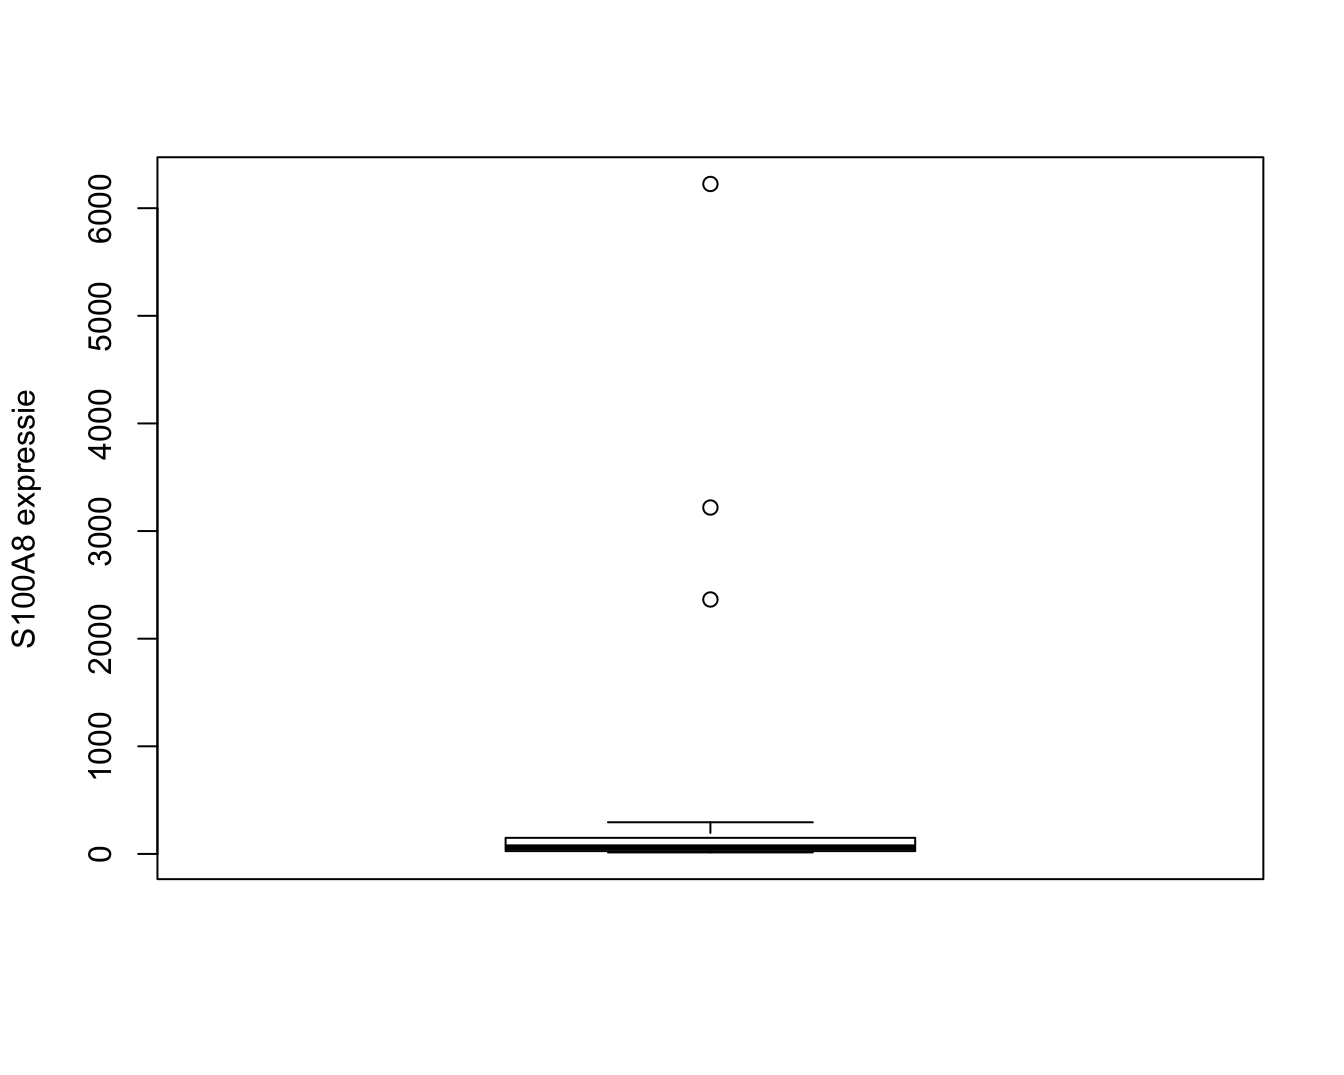
\includegraphics[width=1\linewidth]{Statistiek_2019_2020_files/figure-latex/s100a8Boxplot-1} 

}

\caption{Expressie van het S100A8 gen.}\label{fig:s100a8Boxplot}
\end{figure}

Om meerdere variabelen in de borstkanker dataset te bestuderen, kunnen
we gebruik maken van de grafische scatterplot matrix voorstelling (zie
Figuur \ref{fig:brcaGenAl}). Hierbij wordt een matrix met paarsgewijze
dotplots voor alle variabelen geproduceerd.

\begin{Shaded}
\begin{Highlighting}[]
\KeywordTok{plot}\NormalTok{(}\KeywordTok{subset}\NormalTok{(borstkanker, S100A8 }\OperatorTok{<}\StringTok{ }\DecValTok{2000}\NormalTok{)[, }\OperatorTok{-}\NormalTok{(}\DecValTok{1}\OperatorTok{:}\DecValTok{4}\NormalTok{)])}
\end{Highlighting}
\end{Shaded}

\begin{figure}

{\centering 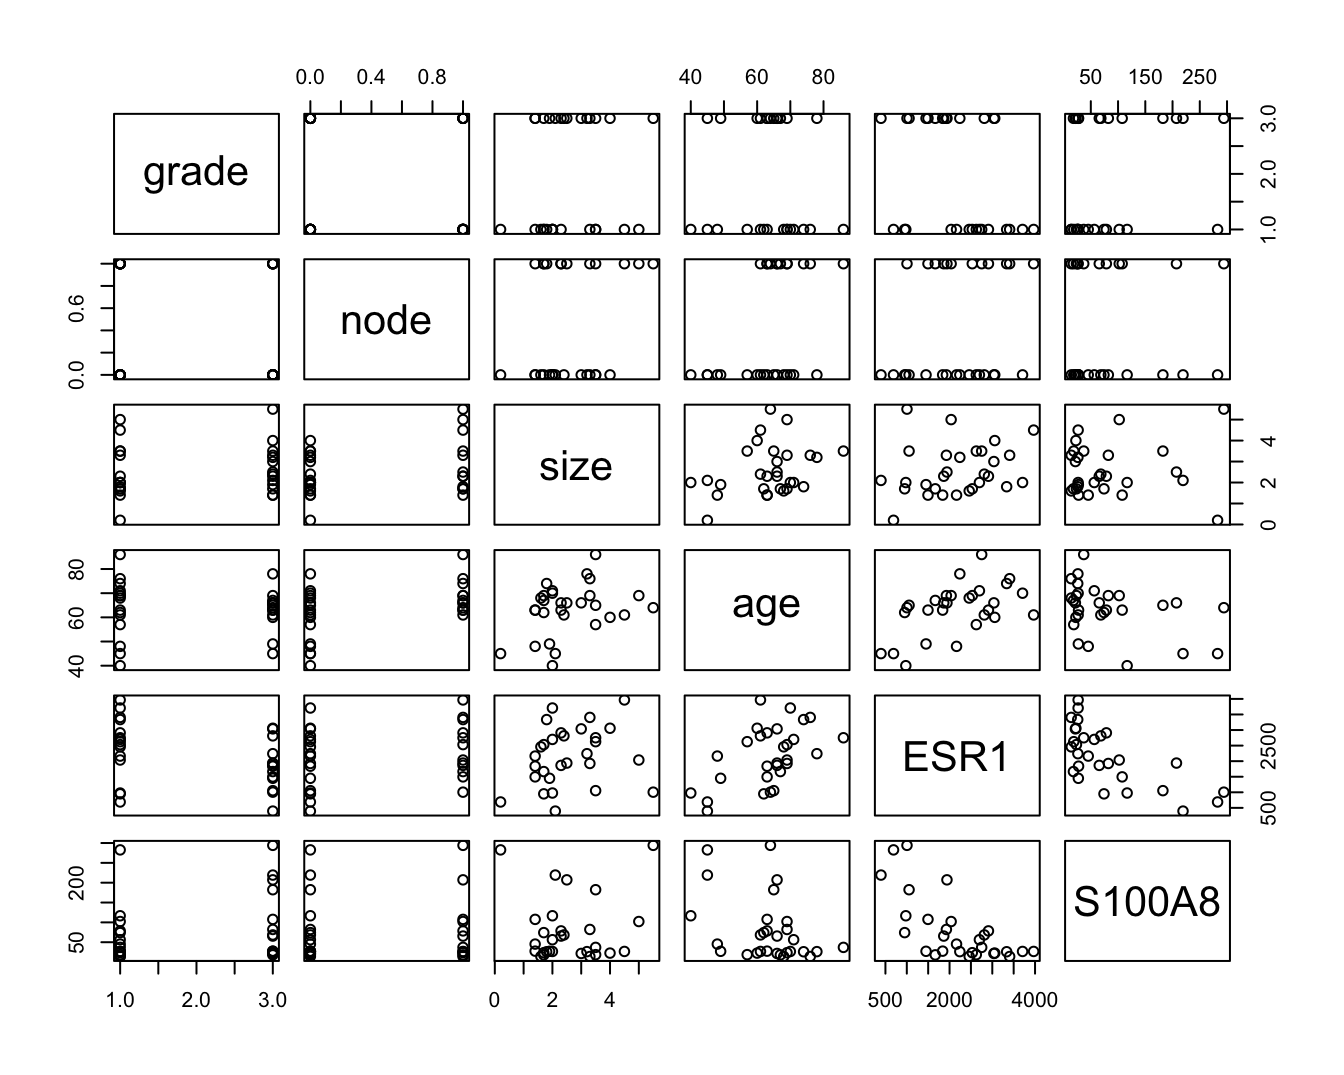
\includegraphics[width=1\linewidth]{Statistiek_2019_2020_files/figure-latex/brcaGenAl-1} 

}

\caption{Scatterplot matrix voor de observaties in de borstkanker dataset na verwijdering van outliers in de S100A8 expressie (merk op dat we deze outliers in principe niet mochten verwijderen uit de dataset).}\label{fig:brcaGenAl}
\end{figure}

In de scatterplot matrix zien we bijvoorbeeld dat er een positieve
associatie lijkt te zijn tussen de leeftijd (age) en de lymfeknoop
status (node; geeft aan of de lymfeknopen al dan niet aangetast zijn en
chirurgisch werden verwijderd, node 0: niet aangetast, 1: aangetast).
Daarnaast observeren we ook een indicatie voor een negatieve associatie
(dalende trend) tussen de ESR1 en S100A8 gen expressie.

In dit hoofdstuk zullen we ons in het bijzonder focussen op de relatie
tussen de ESR1 en de S100A8 gen expressie. Een individuele scatterplot
met smoother (zie Figuur \ref{fig:brcaSmooth}) geeft de associatie
tussen beide genen nog beter weer. Smoothers kunnen trends visualiseren
tussen variabelen zonder vooraf veronderstellingen te doen over de vorm
van het verband en zijn daarom heel erg nuttig bij data exploratie. We
zien dat de genexpressie van S100A8 gemiddeld gezien daalt voor
patiënten met een hogere expressie van ESR1.

\begin{Shaded}
\begin{Highlighting}[]
\KeywordTok{with}\NormalTok{(}\KeywordTok{subset}\NormalTok{(borstkanker, S100A8 }\OperatorTok{<}\StringTok{ }\DecValTok{2000}\NormalTok{), }\KeywordTok{scatter.smooth}\NormalTok{(ESR1, }
\NormalTok{    S100A8))}
\end{Highlighting}
\end{Shaded}

\begin{figure}

{\centering 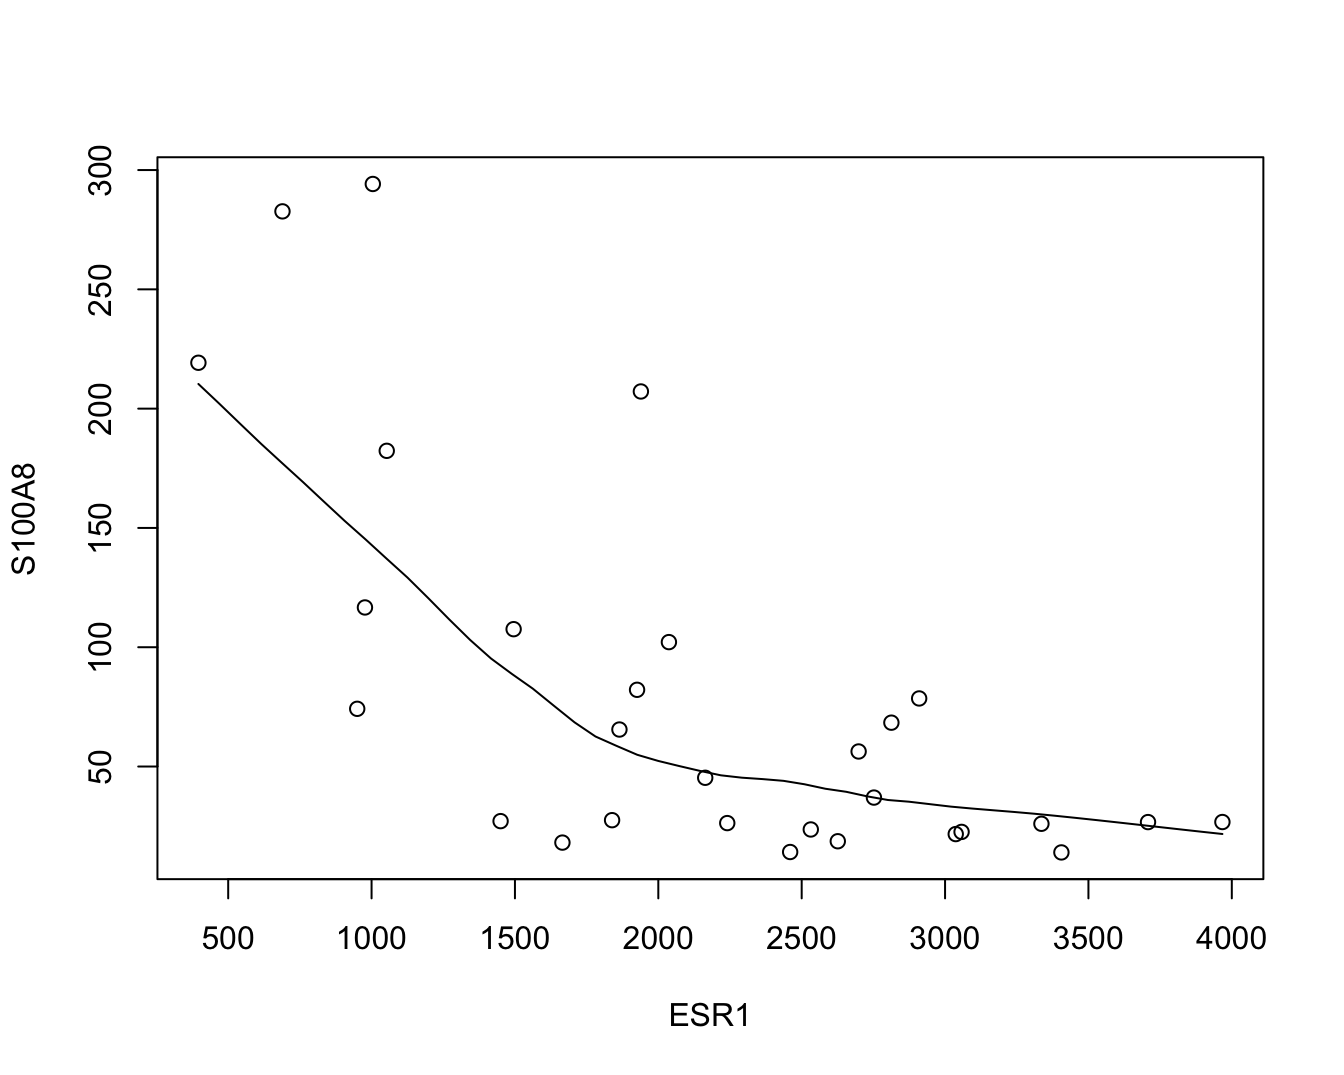
\includegraphics[width=1\linewidth]{Statistiek_2019_2020_files/figure-latex/brcaSmooth-1} 

}

\caption{Scatterplot voor S100A8 expressie in functie van de ESR1 expressie met smoother die het verband tussen beide genen samenvat (na verwijdering van outliers in de S100A8 expressie, merk op dat we deze outliers in principe niet mochten verwijderen uit de dataset).}\label{fig:brcaSmooth}
\end{figure}

\subsection{Model}\label{model}

Op basis van Figuur \ref{fig:brcaSmooth} zien we dat er een relatie is
tussen de S100A8 (Y) en ESR1 (X) expressie. De expressiemetingen voor
het S100A8 gen zijn echter onderhevig aan ruis onder andere door
biologische variabiliteit en technische variabiliteit. Voor een gegeven
waarde \(X=x\) neemt de genexpressie \(Y\) dus niet steeds dezelfde
waarde aan. Generiek kunnen we de S100A8 gen expressie dus beschrijven
als \[\text{observatie = signaal + ruis.}\]

Wiskundig kunnen we dat modelleren als \[Y_i=g(X_i)+\epsilon_i\] waarbij
we de toevallige veranderlijke S100A8 genexpressie voor subject \(i\)
(\(Y_i\)) modelleren in functie van de genexpressie van het ESR1 gen
(\(X_i\)). Uiteraard is dit verband niet perfect. Dat wordt aangegeven
door de foutterm \(\epsilon_i\) die uitdrukt dat observaties \(Y_i\)
variëren rond dit verband, m.a.w. het verband modelleert een
conditioneel gemiddelde: \[E[Y_i|X_i=x]=g(x),\] het is de verwachte
uitkomst\footnote{In de cursus zullen we naar Y refereren met de term
  afhankelijke variable, response variabele of uitkomst, wat 3
  synoniemen zijn} (\(E[Y]\)) bij subjecten met een expressieniveau
\(X_i=x\) voor het ESR1 gen.

Zo geeft \(E(Y|X=2400)\) de gemiddelde genexpressie aan van het S100A8
gen voor subjecten die een expressie hebben van 2400 voor het ESR1 gen.
Men zou dit gemiddelde bekomen door van alle patiënten in de
studiepopulatie, die een ESR1 expressie hebben van 2400, de S100A8
expressie te meten en hier vervolgens het gemiddelde van te nemen. Het
gemiddelde \(E(Y|X=x)\) wordt een \emph{conditioneel gemiddelde} genoemd
omdat het een gemiddelde uitkomst beschrijft, conditioneel op het feit
dat \(X=x\).

Gezien \[E[Y_i|X_i=x]=g(x)\] het gemiddelde beschrijft voor subjecten
met een ESR1 expressieniveau van \(x\) is de foutterm \(\epsilon_i\)
gemiddeld 0 voor deze subjecten: \[E[\epsilon_i\vert X_i=x]=0.\]

\section{Lineaire regressie}\label{lineaire-regressie}

Om accurate en interpreteerbare resultaten te bekomen gaat men vaak
bepaalde veronderstellingen doen over de structuur van \(g(x)\). Zo
modelleert men \(g(x)\) vaak als een lineaire functie van ongekende
parameters. Dat wordt geïllustreerd in Figuur \ref{fig:brcaLin1}.

\begin{Shaded}
\begin{Highlighting}[]
\KeywordTok{plot}\NormalTok{(S100A8 }\OperatorTok{~}\StringTok{ }\NormalTok{ESR1, }\DataTypeTok{data =} \KeywordTok{subset}\NormalTok{(borstkanker, S100A8 }\OperatorTok{<}\StringTok{ }
\StringTok{    }\DecValTok{2000}\NormalTok{))}
\CommentTok{# lm functie fit een linear model abline functie}
\CommentTok{# voegt een lijn toe aan een plot}
\KeywordTok{abline}\NormalTok{(}\KeywordTok{lm}\NormalTok{(S100A8 }\OperatorTok{~}\StringTok{ }\NormalTok{ESR1, }\DataTypeTok{data =} \KeywordTok{subset}\NormalTok{(borstkanker, }
\NormalTok{    S100A8 }\OperatorTok{<}\StringTok{ }\DecValTok{2000}\NormalTok{)))}
\end{Highlighting}
\end{Shaded}

\begin{figure}

{\centering 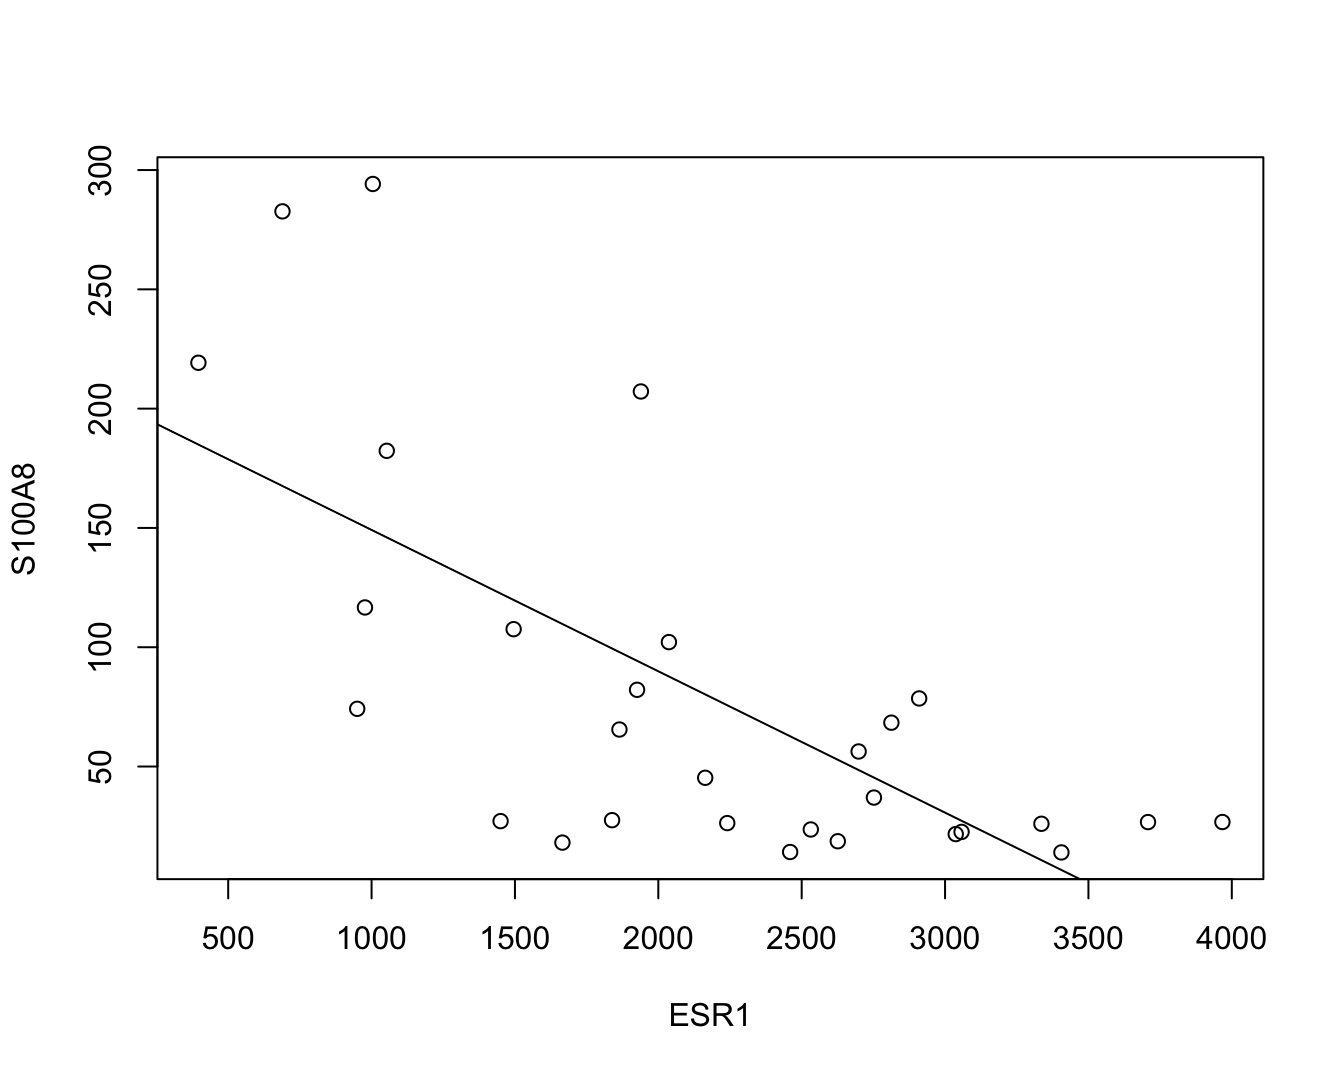
\includegraphics[width=1\linewidth]{Statistiek_2019_2020_files/figure-latex/brcaLin1-1} 

}

\caption{Scatterplot voor S100A8 expressie in functie van de ESR1 expressie met lineair model dat het verband tussen beide genen samenvat (na verwijdering van outliers in de S100A8 expressie, merk op dat we deze outliers in principe niet mochten verwijderen uit de dataset zoals we verder in dit hoofdstuk zullen zien).}\label{fig:brcaLin1}
\end{figure}

Men veronderstelt dan het onderstaande lineaire regressiemodel

\begin{equation} 
E(Y|X =x)=\beta_0 + \beta_1 x  \label{eq:linreg}
\end{equation}

waarbij \(\beta_0\) en \(\beta_1\) onbekende modelparameters zijn. In
deze uitdrukking stelt \(E(Y|X=x)\) de waarde op de \(Y\)-as voor, \(x\)
de waarde op de \(X\)-as, het \emph{intercept} \(\beta_0\) stelt het
snijpunt met de \(Y\)-as voor en de \emph{helling} \(\beta_1\) geeft de
richtingscoëfficiënt van de rechte weer. Uitdrukking \eqref{eq:linreg}
wordt een \emph{statistisch model} genoemd. Merk op dat dit model enkel
een onderstelling maakt over het gemiddelde van de S100A8 expressie.

Deze naamgeving suggereert dat het bepaalde onderstellingen legt op de
verdeling van de geobserveerde gegevens. In het bijzonder onderstelt het
dat de gemiddelde uitkomst lineair varieert in functie van één
verklarende variabele \(X\). Om die reden wordt Model \eqref{eq:linreg}
ook een \emph{enkelvoudig lineair regressiemodel} genoemd. Onder dit
model kan elke meting \(Y\) op een foutterm \(\epsilon\) na beschreven
worden als een lineaire functie van de verklarende variabele \(X\),
verder in deze cursus ook de predictor genoemd:

\[Y=E(Y|X=x)+\epsilon=\beta_0+\beta_1 x+\epsilon\]

waarbij \(\epsilon\) de afwijking tussen de uitkomst en haar
(conditioneel) gemiddelde waarde voorstelt, dit is de onzekerheid in de
responsvariabele.

Gezien het lineair regressiemodel onderstellingen doet over de verdeling
van X en Y , kunnen deze onderstellingen ook vals zijn. Later in dit
hoofdstuk zullen we zien hoe deze onderstellingen geëvalueerd kunnen
worden. Als echter voldaan is aan de onderstellingen, laat dit een
efficiënte data-analyse toe: alle observaties worden benut om te leren
over verwachte uitkomst bij X = x.

Het lineair regressiemodel kan worden gebruikt voor\\
- \emph{predictie} (voorspellingen): als \(Y\) ongekend is, maar \(X\)
wel gekend is, kunnen we \(Y\) voorspellen op basis van \(X\)
\[\text{E}\left[Y|X =x\right]=\beta_0 + \beta_1 x.\] -
\emph{associatie}: beschrijven van de biologische relatie tussen
variabele \(X\) en continue meting \(Y\):

\[\text{E}\left[Y|X=x+\delta\right]-\text{E}\left[Y|X=x\right]= \left[\beta_0+\beta_1(x+\delta)\right]-(\beta_0+\beta_1x)=\beta_1\delta\]

waarbij \(\beta_1\) het verschil is in gemiddelde uitkomst tussen
subjecten die 1 eenheid verschillen in de genexpressie van het ESR1 gen.

\section{Parameterschatting}\label{parameterschatting}

De parameters \(\beta_0\) en \(\beta_1\) zijn onbekenden. Indien de
volledige studiepopulatie geobserveerd werd, dan zouden beide parameters
exact bepaald kunnen worden (door bijvoorbeeld in 2 x-waarden de
gemiddelde uitkomst te berekenen en vervolgens het resulterende stelsel
van 2 vergelijkingen, bepaald door Model \eqref{eq:linreg}, op te lossen).

In de praktijk observeert men slechts een beperkte steekproef uit de
studiepopulatie en is de taak om die parameters te schatten op basis van
de beschikbare observaties. Deze schatting gebeurt door naar de lijn te
zoeken die ``het best past'' bij de gegevens. Daarbij wil men dat bij
een gegeven waarde \(x_i\) voor het \(i\)-de subject het punt op de
regressielijn, \((x_i, \beta_0 + \beta_1 x_i)\), zo weinig mogelijk
afwijkt van de overeenkomstige observatie \((x_i, y_i)\). Dit realiseert
men door deze waarden voor \(\beta_0\) en \(\beta_1\) te kiezen die de
som van die kwadratische afstanden tussen de voorspelde en geobserveerde
punten,

\[\sum_{i=1}^n (y_i-\beta_0-\beta_1 x_i)^2=\sum_{i=1}^n e_i^2\]

zo klein mogelijk maakt. Waarbij \(e_i\) de verticale afstanden van de
observaties tot de gefitte regressierechte, ook wel residuen genoemd
(zie Figuur \ref{fig:brcaLinRes}).

\begin{Shaded}
\begin{Highlighting}[]
\NormalTok{borstkankerSubset <-}\StringTok{ }\KeywordTok{subset}\NormalTok{(borstkanker, S100A8 }\OperatorTok{<}\StringTok{ }\DecValTok{2000}\NormalTok{)}
\KeywordTok{plot}\NormalTok{(S100A8 }\OperatorTok{~}\StringTok{ }\NormalTok{ESR1, borstkankerSubset)}
\NormalTok{lm1 <-}\StringTok{ }\KeywordTok{lm}\NormalTok{(S100A8 }\OperatorTok{~}\StringTok{ }\NormalTok{ESR1, borstkankerSubset)}
\KeywordTok{abline}\NormalTok{(lm1, }\DataTypeTok{col =} \DecValTok{2}\NormalTok{)}
\KeywordTok{points}\NormalTok{(borstkankerSubset}\OperatorTok{$}\NormalTok{ESR1, lm1}\OperatorTok{$}\NormalTok{fitted, }\DataTypeTok{col =} \DecValTok{2}\NormalTok{, }
    \DataTypeTok{pch =} \DecValTok{2}\NormalTok{)}
\ControlFlowTok{for}\NormalTok{ (i }\ControlFlowTok{in} \DecValTok{1}\OperatorTok{:}\KeywordTok{length}\NormalTok{(borstkankerSubset}\OperatorTok{$}\NormalTok{S100A8)) }\KeywordTok{lines}\NormalTok{(}\KeywordTok{rep}\NormalTok{(borstkankerSubset}\OperatorTok{$}\NormalTok{ESR1[i], }
    \DecValTok{2}\NormalTok{), }\KeywordTok{c}\NormalTok{(lm1}\OperatorTok{$}\NormalTok{fitted[i], borstkankerSubset}\OperatorTok{$}\NormalTok{S100A8[i]), }
    \DataTypeTok{lty =} \DecValTok{2}\NormalTok{, }\DataTypeTok{col =} \DecValTok{1}\NormalTok{)}
\KeywordTok{legend}\NormalTok{(}\StringTok{"topright"}\NormalTok{, }\DataTypeTok{lty =} \KeywordTok{c}\NormalTok{(}\DecValTok{0}\NormalTok{, }\DecValTok{2}\NormalTok{, }\DecValTok{0}\NormalTok{, }\DecValTok{1}\NormalTok{), }\DataTypeTok{col =} \KeywordTok{c}\NormalTok{(}\DecValTok{1}\NormalTok{, }
    \DecValTok{1}\NormalTok{, }\DecValTok{2}\NormalTok{, }\DecValTok{2}\NormalTok{), }\DataTypeTok{pch =} \KeywordTok{c}\NormalTok{(}\DecValTok{1}\NormalTok{, }\DecValTok{26}\NormalTok{, }\DecValTok{2}\NormalTok{, }\DecValTok{26}\NormalTok{), }\DataTypeTok{legend =} \KeywordTok{c}\NormalTok{(}\StringTok{"observatie"}\NormalTok{, }
    \StringTok{"residu"}\NormalTok{, }\StringTok{"predictie"}\NormalTok{, }\StringTok{"regressielijn"}\NormalTok{))}
\end{Highlighting}
\end{Shaded}

\begin{figure}

{\centering 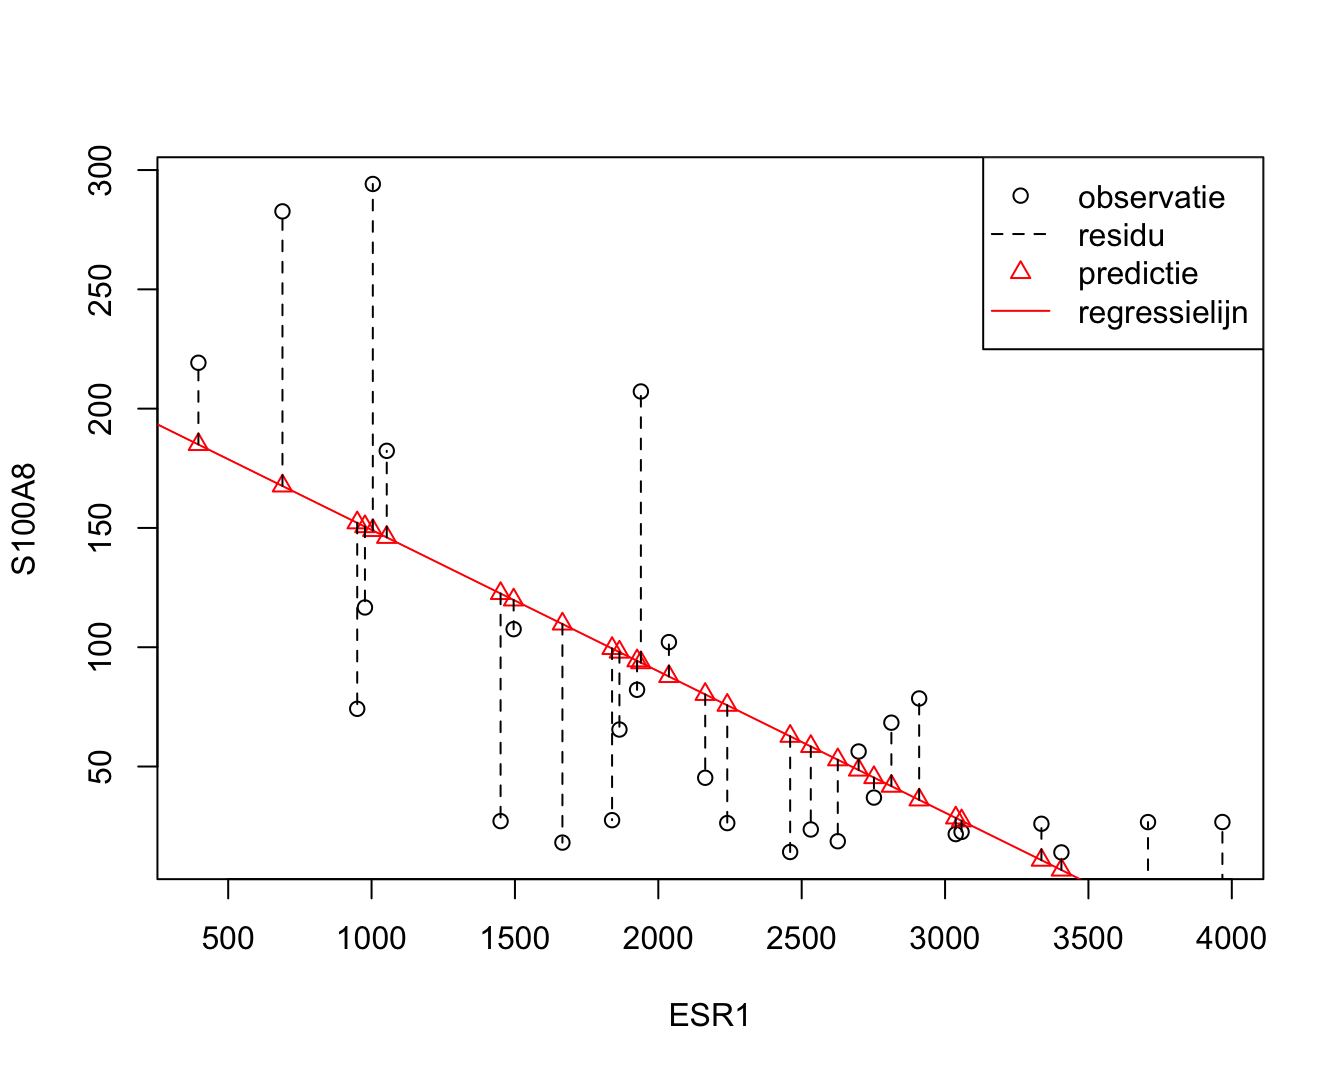
\includegraphics[width=1\linewidth]{Statistiek_2019_2020_files/figure-latex/brcaLinRes-1} 

}

\caption{Scatterplot voor S100A8 expressie in functie van de ESR1 expressie met lineair model en residuen.}\label{fig:brcaLinRes}
\end{figure}

De rechte die men aldus bekomt, noemt men de \emph{kleinste
kwadratenlijn} en is de best passende rechte door de puntenwolk.

De overeenkomstige waarden of schattingen \(\hat{\beta}_0\) voor
\(\beta_0\) en \(\hat{\beta}_1\) voor \(\beta_1\), noemt men
\emph{kleinste kwadratenschattingen}.

Men kan eenvoudig aantonen dat
\[\hat{\beta_1}= \frac{\sum\limits_{i=1}^n (y_i-\bar y)(x_i-\bar x)}{\sum\limits_{i=1}^n (x_i-\bar x_i)^2}=\frac{\mbox{cor}(x,y)s_y}{s_x} \]
en dat

\[\hat{\beta_0}=\bar y - \hat{\beta}_1 \bar x \] Merk op dat de helling
van de kleinste kwadratenlijn evenredig is met de correlatie tussen de
uitkomst en de verklarende variabele.

Voor gegeven schattingen \(\hat{\beta}_0\) voor \(\beta_0\) en
\(\hat{\beta}_1\) voor \(\beta_1\) laat het lineaire regressiemodel
\eqref{eq:linreg} toe om:

\begin{itemize}
\tightlist
\item
  de verwachte uitkomst te voorspellen voor subjecten met een gegeven
  waarde \(x\) voor de verklarende variabele. Deze kan geschat worden
  als \(\hat{\beta}_0+\hat{\beta}_1x\).
\item
  na te gaan hoeveel de uitkomst gemiddeld verschilt tussen 2 groepen
  subjecten met een verschil van \(\delta\) eenheden in de verklarende
  variabele. Namelijk:
\end{itemize}

\[\text{E}\left[Y|X=x+\delta\right]-\text{E}\left[Y|X=x\right]= \hat{\beta}_1\delta\]

Voor de borstkanker dataset levert een analyse van de gegevens in R de
volgende resultaten op.

\begin{Shaded}
\begin{Highlighting}[]
\NormalTok{lm1 <-}\StringTok{ }\KeywordTok{lm}\NormalTok{(S100A8 }\OperatorTok{~}\StringTok{ }\NormalTok{ESR1, borstkankerSubset)}
\KeywordTok{summary}\NormalTok{(lm1)}
\end{Highlighting}
\end{Shaded}

\begin{verbatim}
## 
## Call:
## lm(formula = S100A8 ~ ESR1, data = borstkankerSubset)
## 
## Residuals:
##    Min     1Q Median     3Q    Max 
## -95.43 -34.81  -6.79  34.23 145.21 
## 
## Coefficients:
##              Estimate Std. Error t value Pr(>|t|)    
## (Intercept) 208.47145   28.57207   7.296 7.56e-08 ***
## ESR1         -0.05926    0.01212  -4.891 4.08e-05 ***
## ---
## Signif. codes:  0 '***' 0.001 '**' 0.01 '*' 0.05 '.' 0.1 ' ' 1
## 
## Residual standard error: 59.91 on 27 degrees of freedom
## Multiple R-squared:  0.4698, Adjusted R-squared:  0.4502 
## F-statistic: 23.93 on 1 and 27 DF,  p-value: 4.078e-05
\end{verbatim}

De software rapporteert \(\hat{\beta}_0=\) 208.47 en
\(\hat{\beta}_1=\)-0.059. We besluiten dat, de verwachte S100A8
expressie gemiddeld -59 eenheden lager ligt bij patiënten met een ESR1
expressieniveau die 1000 eenheden hoger ligt. Bovendien kunnen we de
S100A8 expressie voorspellen die men mag verwachten bij een gegeven ESR1
expressieniveau. Bijvoorbeeld, bij een ESR1 expressieniveau van 1300
verwachten we een S100A8 expressieniveau van 208.47 \(-\) 0.059
\(\times\) 1300= 131.43.

Merk op in Figuur \ref{fig:brcaLin1} dat er in de dataset geen patiënt
is geobserveerd die een ESR1 expressieniveau had van 1300. Op basis van
de dataset zou het bijgevolg niet mogelijk zijn om, zonder gebruik te
maken van een statistisch model, een schatting te bekomen voor de S100A8
expressie bij deze ESR1 expressiewaarde. Onder de veronderstelling dat
de gemiddelde S100A8 expressie lineair varieert in functie van de ESR1
expressie, kunnen we alle observaties gebruiken om dit gemiddelde te
schatten. Bijgevolg bekomen we een zinvol en precies resultaat, op
voorwaarde dat aan de veronderstelling van lineariteit is voldaan. Het
zal bijgevolg belangrijk zijn om de veronderstelling van lineariteit na
te gaan (zie verder).

Gezien de lineariteit van het model enkel kan worden nagegaan over het
geobserveerde bereik van de verklarende variabele (bijvoorbeeld, over
het interval 396.1,3967.2), is het belangrijk om te begrijpen dat de
resultaten van een lineair regressiemodel niet zomaar kunnen
geëxtrapoleerd worden voorbij de kleinste of grootste geobserveerde
\(X\)-waarde. Met het model kunnen we de verwachte S100A8 intensiteit
voor patiënten met een ESR1 expressie-niveau van 4500 schatten, maar de
geobserveerde data laten niet toe om na te gaan of dit een betrouwbare
schatting is. Het zou immers kunnen dat de regressielijn bij hoge
waarden van de predictorvariabele afbuigt of opklimt waardoor een
lineaire extrapolatie misleidend zou zijn. Merk zo bijvoorbeeld op dat
predictie bij een ESR1 intensiteit van 4500 bijzonder misleidend is
vermits ze een negatief resultaat oplevert wat onmogelijk is voor een
intensiteitsmeting (208.47 \(+\) -0.059 \(\times\) 4500= -58.22).

\section{Statistische besluitvorming}\label{sec:linBesluit}

Als de gegevens representatief zijn voor de populatie kan men in de
regressiecontext eveneens aantonen dat de kleinste kwadraten schatters
voor het intercept en de helling onvertekend zijn, m.a.w
\[E[\hat \beta_0]=\beta_0 \text{ en } E[\hat \beta_1]=\beta_1\] Het feit
dat de schatters gemiddeld (over een groot aantal vergelijkbare studies)
niet afwijken van de waarden in de populatie, impliceert niet dat ze
niet rond die waarde variëren. Om inzicht te krijgen hoe dicht we de
parameterschatters bij het werkelijke intercept \(\beta_0\) en de
werkelijke helling \(\beta_1\) mogen verwachten, wensen we bijgevolg ook
haar variabiliteit te kennen.

In de borstkanker dataset hebben we een negatieve associatie
geobserveerd tussen de S100A8 en ESR1 gen expressie. Net zoals in
Hoofdstuk \ref{chap:besluit} is het op basis van de puntschatters voor
de helling niet duidelijk of dat verband werkelijk voorkomt in de
populatie of indien we het verband door toeval hebben geobserveerd in de
dataset. De schatting van de helling is immers onnauwkeurig en zal
variëren van steekproef tot steekproef. Het resultaat van een
data-analyse is dus niet interpreteerbaar zonder die variabiliteit in
kaart te brengen.

Om de resultaten uit de steekproef te kunnen veralgemenen naar de
populatie zullen we in deze context eveneens inzicht nodig hebben op de
verdeling van de parameterschatters. Om te kunnen voorspellen hoe de
parameterschatters variëren van steekproef tot steekproef enkel en
alleen op basis van slechts één steekproef zullen we naast de
onderstelling van

\begin{enumerate}
\def\labelenumi{\arabic{enumi}.}
\tightlist
\item
  \emph{Lineariteit}
\end{enumerate}

bijkomende aannames moeten maken over de verdeling van de gegevens, met
name

\begin{enumerate}
\def\labelenumi{\arabic{enumi}.}
\setcounter{enumi}{1}
\tightlist
\item
  \emph{Onafhankelijkheid}: de metingen \((X_1,Y_1), ..., (X_n,Y_n)\)
  werden gemaakt bij n onafhankelijke subjecten/observationele eenheden
\item
  \emph{Homoscedasticiteit} of \emph{gelijkheid van variantie}: de
  observaties variëren met een gelijke variantie rond de
  regressierechte. De residuen \(\epsilon_i\) hebben dus een gelijke
  variantie \(\sigma^2\) voor elke \(X_i=x\). Dat impliceert ook dat de
  conditionele variantie van Y gegeven X\footnote{Analoog aan het
    conditionele gemiddelde \(E(Y|X=x)\), geeft
    \(\text{var}(Y\vert X=x) = \sigma^2\) de variantie weer op de
    uitkomsten voor de subgroep van de studiepopulatie bestaande uit
    subjecten met een ESR1 gen expressie gelijk aan \(x\).},
  \(\text{var}(Y\vert X=x)\) dus gelijk is, met name
  \(\text{var}(Y\vert X=x) = \sigma^2\) voor elke waarde \(X=x\). De
  constante \(\sigma\) wordt ook de \emph{residuele standaarddeviatie}
  genoemd.
\item
  \emph{Normaliteit}: de residuen \(\epsilon_i\) zijn normaal verdeeld.
\end{enumerate}

Uit 2, 3 en 4 volgt dus dat de residuen \(\epsilon_i\) onafhankelijk
zijn en dat ze allen eenzelfde Normale verdeling volgen
\[\epsilon_i \sim N(0,\sigma^2).\] Als we ook steunen op de
veronderstelling van lineariteit weten we dat de originele observaties
conditioneel op \(X\) eveneens Normaal verdeeld zijn
\[Y_i\sim N(\beta_0+\beta_1 X_i,\sigma^2),\] met een gemiddelde dat
varieert in functie van de waarde van de onafhankelijke variabele
\(X_i\).

Verder kan men aantonen dat onder deze aannames
\[\sigma^2_{\hat{\beta}_0}=\frac{\sum\limits_{i=1}^n X^2_i}{\sum\limits_{i=1}^n (X_i-\bar X)^2} \times\frac{\sigma^2}{n} \text{ en } \sigma^2_{\hat{\beta}_1}=\frac{\sigma^2}{\sum\limits_{i=1}^n (X_i-\bar X)^2}\]
en dat de parameterschatters eveneens normaal verdeeld zijn
\[\hat\beta_0 \sim N\left(\beta_0,\sigma^2_{\hat \beta_0}\right) \text{ en } \hat\beta_1 \sim N\left(\beta_1,\sigma^2_{\hat \beta_1}\right)\]

Merk op dat de onzekerheid op de helling af zal nemen wanneer er meer
observaties zijn en/of wanneer de observaties meer gespreid zijn. Voor
het opzetten van een experiment kan dit belangrijke informatie zijn.
Uiteraard wordt de precisie ook beïnvloed door de grootte van de
variabiliteit van de observaties rond de rechte, \(\sigma^2\), maar dat
heeft een onderzoeker meestal niet in de hand.

De conditionele variantie (\(\sigma^2\)) is echter niet gekend en is
noodzakelijk voor de berekening van de variantie op de
parameterschatters. We kunnen \(\sigma^2\) echter ook schatten op basis
van de observaties. Zoals beschreven in Hoofdstuk \ref{chap:describe}
kunnen we de variatie van de uitkomsten rond hun conditionele gemiddelde
beschrijven d.m.v. de afwijkingen tussen de observaties \(y_i\) en hun
(geschatte) gemiddelde \(\hat{g}(x)=\hat{\beta}_0+\hat{\beta}_1x_i\), de
residu's. Het gemiddelde van die residu's is echter altijd 0 omdat
positieve en negatieve residu's mekaar opheffen. Bijgevolg levert het
gemiddelde residu geen goede maat op voor de variatie en is het beter om
naar kwadratische afwijkingen \(e_i^2\) te kijken. Net zoals de
steekproefvariantie een goede schatter was voor de variantie (Sectie
\ref{subsec:spreiding}), zal in de regressiecontext het gemiddelde van
die kwadratische afwijkingen rond de regressierechte opnieuw een goede
schatter zijn voor \(\sigma^2\). Deze schatter wordt in de literatuur
ook wel de \emph{mean squared error} (MSE) genoemd.
\[\hat\sigma^2=MSE=\frac{\sum\limits_{i=1}^n \left(y_i-\hat\beta_0-\hat\beta_1\times x_i\right)^2}{n-2}=\frac{\sum\limits_{i=1}^n e^2_i}{n-2}.\]
Voor het bekomen van deze schatter steunen we op onafhankelijkheid
(aanname 2) en homoscedasticiteit (aanname 3). Merk op dat we bij deze
schatter niet delen door het aantal observaties \(n\), maar door
\(n-2\). Hierbij corrigeren we voor het feit dat voor de berekening van
MSE 2 vrijheidsgraden worden gespendeerd aan het schatten van het
intercept en de helling.

Na het schatten van MSE kunnen we \(\sigma^2\) door MSE vervangen zodat
schatters worden bekomen voor de variantie en standard error op de
schatters van model parameters,
\[\text{SE}_{\hat{\beta}_0}=\hat\sigma_{\hat{\beta}_0}=\sqrt{\frac{\sum\limits_{i=1}^n X^2_i}{\sum\limits_{i=1}^n (X_i-\bar X)^2} \times\frac{\text{MSE}}{n}} \text{ en } \text{SE}_{\hat{\beta}_1}=\hat\sigma_{\hat{\beta}_1}=\sqrt{\frac{\text{MSE}}{\sum\limits_{i=1}^n (X_i-\bar X)^2}}\]

Analoog als in Hoofdstuk \ref{chap:besluit} kunnen we opnieuw toetsen en
betrouwbaarheidsintervallen construeren op basis van de
teststatistieken\\
\[T=\frac{\hat{\beta}_k-\beta_k}{SE(\hat{\beta}_k)} \text{ met } k=1,2.\]
Als aan alle aannames is voldaan dan volgen deze statistieken \(T\) een
t-verdeling met n-2 vrijheidsgraden. Wanneer niet is voldaan aan de
veronderstelling van normaliteit maar wel aan lineariteit,
onafhankelijkheid en homoscedasticiteit dan kunnen we voor inferentie
opnieuw beroep doen op de centrale limietstelling die zegt dat de
statistiek T bij benadering een standaard Normaal verdeling zal volgen
wanneer het aantal observaties voldoende groot is.

In de borstkanker dataset hebben we een negatieve associatie
geobserveerd tussen de S100A8 en ESR1 gen expressie. We kunnen het
effect in de steekproef nu veralgemenen naar de populatie toe door een
betrouwbaarheidsinterval te bouwen voor de helling:
\[[\hat\beta_1 - t_{n-2,\alpha/2} \text{SE}_{\hat\beta_1},\hat\beta_1 + t_{n-2,\alpha/2} \text{SE}_{\hat\beta_1}]\].

\begin{Shaded}
\begin{Highlighting}[]
\KeywordTok{confint}\NormalTok{(lm1)}
\end{Highlighting}
\end{Shaded}

\begin{verbatim}
##                    2.5 %       97.5 %
## (Intercept) 149.84639096 267.09649989
## ESR1         -0.08412397  -0.03440378
\end{verbatim}

Op basis van de R-output bekomen we een 95\% betrouwbaarheidsinterval
voor de helling {[}-0.084,-0.034{]}. Gezien nul niet in het interval
ligt weten we eveneens dat de negatieve associatie statistisch
significant is op het 5\% significantieniveau.

Anderzijds kunnen we ook een formele hypothesetoets uitvoeren. Onder de
nulhypothese veronderstellen we dat er geen associatie is tussen de
expressie van beide genen: \[H_0: \beta_1=0\] en onder de alternatieve
hypothese is er een associatie tussen beide genen: \[H_1: \beta_1\neq0\]

Met de test statistiek \[T=\frac{\hat{\beta}_1-0}{SE(\hat{\beta}_k)}\]
kunnen we de nulhypothese falsifiëren. Onder \(H_0\) volgt de statistiek
een t-verdeling met n-2 vrijheidsgraden.

Deze tweezijdige test is geïmplementeerd in de standaard output van R.

\begin{Shaded}
\begin{Highlighting}[]
\KeywordTok{summary}\NormalTok{(lm1)}
\end{Highlighting}
\end{Shaded}

\begin{verbatim}
## 
## Call:
## lm(formula = S100A8 ~ ESR1, data = borstkankerSubset)
## 
## Residuals:
##    Min     1Q Median     3Q    Max 
## -95.43 -34.81  -6.79  34.23 145.21 
## 
## Coefficients:
##              Estimate Std. Error t value Pr(>|t|)    
## (Intercept) 208.47145   28.57207   7.296 7.56e-08 ***
## ESR1         -0.05926    0.01212  -4.891 4.08e-05 ***
## ---
## Signif. codes:  0 '***' 0.001 '**' 0.01 '*' 0.05 '.' 0.1 ' ' 1
## 
## Residual standard error: 59.91 on 27 degrees of freedom
## Multiple R-squared:  0.4698, Adjusted R-squared:  0.4502 
## F-statistic: 23.93 on 1 and 27 DF,  p-value: 4.078e-05
\end{verbatim}

De test geeft weer dat de associatie tussen de S100A8 en ESR1
genexpressie extreem significant is (p\textless{}\textless{}0.001). Als
de nulhypothese waar is en als aan alle voorwaarden is voldaan dan is er
een kans van 4 op 100000 om een helling te vinden die minstens even
extreem is door toeval. Het is bijgevolg heel onwaarschijnlijk om
dergelijke associatie te observeren in een steekproef wanneer de
nulhypothese waar is.

Vooraleer we een conclusie trekken is het echter belangrijk dat we alle
aannames verifiëren omdat de statistische test en de
betrouwbaarheidsintervallen anders incorrect zijn.

\section{Nagaan van
modelveronderstellingen}\label{nagaan-van-modelveronderstellingen}

Voor de statistische besluitvorming hebben we volgende aannames gedaan

\begin{enumerate}
\def\labelenumi{\arabic{enumi}.}
\tightlist
\item
  Lineariteit
\item
  Onafhankelijkheid\\
\item
  Homoscedasticiteit
\item
  Normaliteit
\end{enumerate}

Onafhankelijkheid is moeilijk te verifiëren op basis van de data, dat
zou gegarandeerd moeten zijn door het design van de studie. Als we
afwijkingen zien van lineariteit dan heeft besluitvorming geen zin
gezien het de primaire veronderstelling is. In dat geval moeten we het
conditioneel gemiddeld eerst beter modelleren. In geval van lineariteit
maar schendingen van homoscedasticiteit of normaliteit dan weten we dat
de besluitvorming mogelijks incorrect is omdat de teststatistiek dan
niet langer een t-verdeling volgt.

\subsection{Lineariteit}\label{lineariteit}

De primaire veronderstelling in lineaire regressie-analyse is de aanname
dat de uitkomst (afhankelijke variabele) lineair varieert ten opzichte
van de verklarende variabele. Deze veronderstelling kan men gemakkelijk
grafisch verifiëren op basis van een scatterplot waarbij men de uitkomst
uitzet in functie van de verklarende variabele. Vervolgens gaat men na
of het verband een lineair patroon volgt.\\
In Figuur \ref{fig:brcaLin1} zien we systematische afwijkingen bij
kleine en grote waarden voor de ESR1 expressie. De observaties liggen
dan steeds systematisch boven de regressierechte wat aangeeft dat het
gemiddelde in deze regio's systematisch wordt onderschat. Afwijkingen
van lineariteit worden vaak echter makkelijker opgespoord d.m.v. een
\emph{residuplot}. Dit is een scatterplot met de verklarende variabele
op de \(X\)-as en de \emph{residuen} op de \(Y\)-as
\[e_i=y_i-\hat{g}(x_i)=y_i-\hat\beta_0-\hat\beta_1\times x_i,\] deze
werden weergegeven in Figuur \ref{fig:brcaLinRes}.

Als de veronderstelling van lineariteit opgaat, krijgt men in een
residuplot geen patroon te zien. De residuen zijn immers gemiddeld nul
voor elke waarde van de predictor en zouden dus mooi rond nul moeten
variëren.

Wanneer de residu's echter een niet-lineair patroon onthullen, dan geeft
dit aan dat extra termen in het model moeten worden opgenomen om de
gemiddelde uitkomst correct te voorspellen. Bijvoorbeeld, wanneer de
residu's een kwadratisch patroon onthullen, dan kunnen we schrijven dat
bij benadering \(e_i\approx \delta_0+\delta_1 x_i+\delta_2 x_i^2\) voor
zekere getallen \(\delta_0,\delta_1,\delta_2\), en bijgevolg dat de
uitkomst
\(y_i=\hat{\alpha}+\hat{\beta}x_i+e_i\approx (\hat{\alpha}+\delta_0)+(\hat{\beta}+\delta_1)x_i+\delta_2 x_i^2\)
(op een foutterm na) een kwadratische functie is van \(x_i\). In dat
geval is het aangewezen om op een kwadratisch regressiemodel over te
stappen (zie Hoofdstuk \ref{chap:glm}). Residuplots worden standaard
gegenereerd door de R-software. Hier worden de residuen echter geplot
ten opzichte van de gefitte waarden wat eenvoudiger is wanneer meerdere
predictoren in het model worden opgenomen (zie Hoofdstuk
\ref{chap:glm}).

\begin{Shaded}
\begin{Highlighting}[]
\KeywordTok{par}\NormalTok{(}\DataTypeTok{mfrow =} \KeywordTok{c}\NormalTok{(}\DecValTok{2}\NormalTok{, }\DecValTok{2}\NormalTok{))}
\KeywordTok{plot}\NormalTok{(lm1)}
\end{Highlighting}
\end{Shaded}

\begin{figure}

{\centering 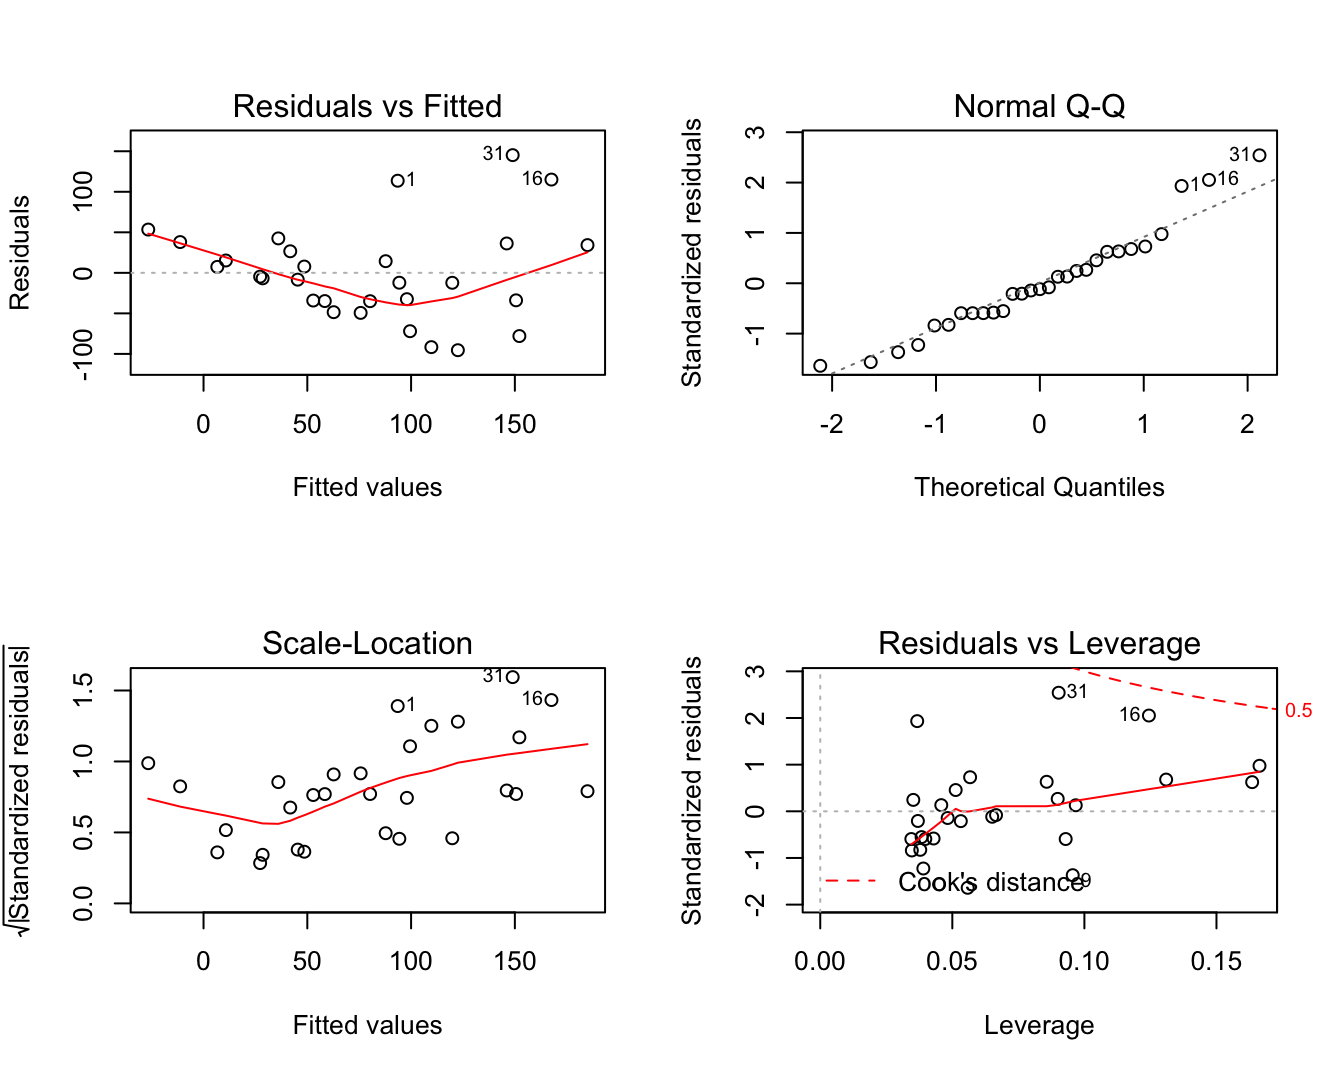
\includegraphics[width=1\linewidth]{Statistiek_2019_2020_files/figure-latex/brcaLinDiag1-1} 

}

\caption{Diagnostische plots voor het nagaan van de veronderstellingen van het lineair regressiemodel waarbij de S100A8 expressie wordt gemodelleerd i.f.v de ESR1 expressie (na verwijdering van 3 outliers).}\label{fig:brcaLinDiag1}
\end{figure}

De residu plot voor het borstkanker voorbeeld wordt weergegeven in
Figuur \ref{fig:brcaLinDiag1} boven links. De residuen zijn niet overal
mooi gespreid rond nul. Bij lage en hoge voorspelde waarden voor het
model (dus bij hoge en lage waarden voor de predictor, negatieve
helling) zijn de residuen overwegend positief wat opnieuw aangeeft dat
het model de data in deze regio's systematisch onderschat. Dat was
ergens te verwachten gezien de smoother in Figuur \ref{fig:brcaSmooth}
immers eerder een exponentiëel verband suggereerde. Bovendien voorspelde
het regressiemodel eveneens negatieve waarden voor de S100A8 expressie
wat onmogelijk is voor intensiteitsmetingen die immers steeds positief
zijn.

\subsection{Veronderstelling van homoscedasticiteit (gelijkheid van
variantie)}\label{veronderstelling-van-homoscedasticiteit-gelijkheid-van-variantie}

Residuen en kwadratische residu's dragen informatie in zich over
residuele variabiliteit. Als er homoscedasiticiteit is dan verwachten we
dat de residuen eenzelfde spreiding hebben voor elke waarde van de
predictor en voor elke predictie. Als de spreiding in de residuen
geassocieerd zijn met de verklarende variabelen, dan is er indicatie van
heteroscedasticiteit. De diagnostische plots van het software pakket R
geven een residu-plot weer en een plot van de vierkantswortel van de
absolute waarde van de gestandardiseerde error
\(\sqrt{|e_i|/\sqrt{MSE}}\) in functie van de predicties. De residu-plot
voor het borstkanker voorbeeld Figuur \ref{fig:brcaLinDiag1} boven links
geeft afwijkingen weer van homoscedasiticiteit. De spreiding in de
residuen lijkt toe te nemen met een toenemende waarde van de predictor.
De plot beneden links is specifiek om de voorwaarde van gelijkheid van
variantie na te gaan en geeft eveneens aan dat de variantie toeneemt met
het conditioneel gemiddelde. Een dergelijke trend komt dikwijls voor bij
concentratiemetingen en intensiteitsmetingen, die vaak een
multiplicatieve errorstructuur vertonen i.p.v. een additieve error.

Voor bepaalde types uitkomsten bestaan er \emph{variantie-stabiliserende
transformaties} voor de afhankelijke variabele die erop gericht zijn om
de onderstelling van homoscedasticiteit te doen opgaan. Voor proporties
of percentages, gebruikt men bijvoorbeeld vaak de arcsin-transformatie
die de uitkomst \(Y\) omzet in \(\arcsin\sqrt{Y}\), omdat men kan
aantonen dat percentages (onder bepaalde onderstellingen) een constante
variantie hebben na deze transformatie. Voor concentraties en
intensiteitsmetingen gebruikt men dan weer vaak een logaritmische
transformatie gezien deze (a) positief zijn, (b) vaak gekenmerkt worden
door een variantie die toeneemt met het gemiddelde en (c) veelal een
scheve verdeling vertonen maar rechts. Indien transformatie van de
uitkomst niet helpt of niet wenselijk is (bijvoorbeeld, omdat het de
interpretatie van het model niet ten goede komt) en er is een consistent
patroon van ongelijke variantie (bijvoorbeeld, toenemende variantie in
uitkomst bij toenemende predictorwaarden), dan kan men ook \emph{gewogen
kleinste kwadratenschatters} (in het Engels: \emph{weighted least
squares}) bepalen. Een verder alternatief is om \emph{veralgemeende
lineaire modellen} (in het Engels: \emph{generalized linear models}) te
schatten die tevens andere verdelingen voor de uitkomst dan de Normale
verdeling toelaten. Beide klassen van oplossingen (d.i. gewogen kleinste
kwadratenschatters en veralgemeende lineaire modellen) vallen echter
buiten het bestek van deze cursus.

\subsection{Veronderstelling van
normaliteit}\label{veronderstelling-van-normaliteit}

Opnieuw kunnen we de veronderstelling van normaliteit nagaan door
gebruik te maken van QQ-plots. Een QQ-plot van de afhankelijke variabele
is misleidend omdat deze nagaat of de metingen voor alle subjecten samen
Normaal verdeeld zijn. Dat is echter niet het geval gezien de normale
verdeling per subject varieert. Elk subject kan immers andere waarde
hebben voor de predictor \(X\) (ESR1 expressie) en bijgevolg hebben ze
een verschillend conditioneel gemiddelde. Normaal verdeelde uitkomsten
bij gegeven \(x\)-waarde impliceert echter dat de residu's bij
benadering Normaal verdeeld zijn. Afwijkingen van Normaliteit in een
QQ-plot van de residu's levert dus een indicatie dat de uitkomsten niet
Normaal verdeeld zijn bij vaste \(x\).

Figuur \ref{fig:brcaLinDiag1} rechts boven geeft de QQ-plot weer van de
residuen voor het borstkanker voorbeeld. We zien wat afwijkingen in de
rechterstaart die wijzen op meerdere outliers of op observaties die
systematisch hoger liggen dan wat verwacht kan worden op basis van de
normaalverdeling. Dit is niet verrassend omdat heterogeniteit van de
variantie vaak samengaat met niet-Normaliteit, i.h.b. scheefheid, van de
gegevens. Dat komt vaak voor bij concentratie- en intensiteitsmetingen.

\section{Afwijkingen van
Modelveronderstellingen}\label{afwijkingen-van-modelveronderstellingen}

De primaire onderstelling in lineaire regressie-analyse is de aanname
dat de uitkomst lineair varieert in de predictor. Wanneer residuplots
suggereren dat aan deze onderstelling niet is voldaan, dan kan men
overwegen om de verklarende variabele te transformeren. In genexpressie
studies waarbij expressie als een covariaat wordt gebruikt om een andere
variabele te verklaren, is het bijvoorbeeld vaak zo dat de (gemiddelde)
uitkomst niet lineair varieert in functie van de predictor, maar wel in
functie van het logaritme van de genexpressie. In dat geval kan men
ervoor kiezen om de log-transformatie van de verklarende variabele als
predictor in het model op te nemen. Vaak wordt in expressie studies een
\(\log_2\) transformatie gebruikt. In andere voorbeelden kan een andere
transformatie dan de log-transformatie beter geschikt zijn, zoals de
vierkantswortel (\(\sqrt{x}\)) of inverse (\(1/x\)) transformatie.

Een transformatie van de verklarende variabele is vaak makkelijk uit te
voeren, maar bemoeilijkt wel vaak de interpretatie van de parameters in
het model. Dit laatste is echter niet het geval wanneer de
log-transformatie wordt gebruikt, een stijging in \(log_2\)-expressie
met bijvoorbeeld 1 eenheid is immers equivalent met een wijziging in
genexpressie met een factor \(2^1=2\). Kenmerkend aan transformatie van
de verklarende variabele is dat ze geen rechtstreekse invloed heeft op
de homogeniteit van de variantie en de Normaliteit van de uitkomst (bij
vaste waarden van de predictorvariabele), tenzij door het verbeteren van
de lineariteit van het model. Om die reden is deze optie vaak minder
geschikt wanneer er sterke afwijkingen van Normaliteit zijn.

Een alternatieve mogelijkheid om de lineariteit van het model te
verbeteren, is hogere orde regressie (in het Engels: \emph{higher order
regression}. Hierbij modelleert men rechtstreeks niet-lineaire relaties
door hogere orde termen in het model op te nemen. Zo kan men
bijvoorbeeld een tweede orde model beschouwen:
\[E(Y|X)=\beta_0+\beta_1X+\beta_2X^2\] zodat de regressiekromme eruit
ziet als een parabool, of een derde orde model:
\[E(Y|X)=\beta_0+\beta_1X+\beta_2X^2+\beta_3X^3\] zodat de
regressiekromme een derdegraadspolynoom is. Deze methode kan gezien
worden als een vorm van transformatie van de verklarende variabele en
bezit wezenlijk dezelfde eigenschappen en voor- en nadelen. Een
bijkomend voordeel is echter dat het hier niet nodig is om zelf een
transformatie te zoeken, maar dat de methode zelf impliciet een goede
polynoom als transformatie schat.

Tenslotte kan men ook overwegen om, in plaats van de verklarende
variabele, de uitkomst te transformeren. Bijvoorbeeld, wanneer de
uitkomsten scheef verdeeld zijn naar rechts is het vaak aangewezen om
een log-transformatie van de uitkomst uit te voeren en deze nieuwe
variabele als uitkomst in het model op te nemen. Doorgaans verbetert dit
niet alleen de lineariteit van het model, maar maakt het ook de residu's
beter Normaal verdeeld met een meer constante variabiliteit. Deze
methode heeft dezelfde voor- en nadelen als transformatie van de
verklarende variabele. Een groot verschil dat de keuze tussen beide
methoden beïnvloedt is dat transformaties van de onafhankelijke
variabele weinig of geen invloed hebben op de verdeling van de residu's
(tenzij via wijzigingen in hun gemiddelde) in tegenstelling tot
transformaties van de afhankelijke variabele. In het bijzonder blijven
Normaal verdeelde residu's vrij Normaal verdeeld na transformatie van de
verklarende variabele, terwijl ze mogelijks niet langer Normaal verdeeld
zijn na transformatie van de uitkomst, en vice versa.

In het borstkanker voorbeeld wordt de S100A8 genexpressie gemodelleerd
in functie van de ESR1 genexpressie. Er waren problemen m.b.t.
heteroscedasticiteit, mogelijkse afwijking van normaliteit (scheefheid
naar rechts), negatieve concentratievoorspellingen die theoretisch niet
mogelijk zijn en niet-lineairiteit. Dergelijke problemen treden veelal
op bij concentratie en intensiteitsmetingen. Deze zijn vaak log-normaal
verdeeld (normale verdeling na log-transformatie) en worden daarom vaak
log-getransformeerd. Bovendien zagen we in Figuur \ref{fig:brcaSmooth}
eveneens een soort exponentiële trend. In de genexpressie literatuur
wordt veelal gebruik gemaak van \(\log_2\) transformatie gezien een
verschil van 1 op log-schaal een verdubbeling impliceert in de expressie
op de originele schaal. Wanneer men gen-expressie op log-schaal
modelleert, modellert men dus in feite proportionele verschillen op de
originele schaal wat ook meer relevant is vanuit een biologisch
standpunt.

In deze sectie zullen we beide genexpressies \(\log_2\) transformeren en
een log-lineaire regressie uitvoeren. Zoals we zullen zien vormen de
outliers in de S100A8 expressie na log-transformatie ook geen problemen
meer.

\begin{Shaded}
\begin{Highlighting}[]
\NormalTok{borstkanker}\OperatorTok{$}\NormalTok{log2S100A8 <-}\StringTok{ }\KeywordTok{log2}\NormalTok{(borstkanker}\OperatorTok{$}\NormalTok{S100A8)}
\NormalTok{borstkanker}\OperatorTok{$}\NormalTok{log2ESR1 <-}\StringTok{ }\KeywordTok{log2}\NormalTok{(borstkanker}\OperatorTok{$}\NormalTok{ESR1)}
\NormalTok{lm2 <-}\StringTok{ }\KeywordTok{lm}\NormalTok{(log2S100A8 }\OperatorTok{~}\StringTok{ }\NormalTok{log2ESR1, borstkanker)}
\KeywordTok{with}\NormalTok{(borstkanker, }\KeywordTok{scatter.smooth}\NormalTok{(log2ESR1, log2S100A8, }
    \DataTypeTok{lpars =} \KeywordTok{list}\NormalTok{(}\DataTypeTok{lty =} \DecValTok{2}\NormalTok{)))}
\KeywordTok{abline}\NormalTok{(lm2)}
\KeywordTok{legend}\NormalTok{(}\StringTok{"topright"}\NormalTok{, }\DataTypeTok{lty =} \DecValTok{1}\OperatorTok{:}\DecValTok{2}\NormalTok{, }\DataTypeTok{legend =} \KeywordTok{c}\NormalTok{(}\StringTok{"Lineair model"}\NormalTok{, }
    \StringTok{"Smoother"}\NormalTok{))}
\end{Highlighting}
\end{Shaded}

\begin{figure}

{\centering \includegraphics[width=1\linewidth]{Statistiek_2019_2020_files/figure-latex/brcaLogLin-1} 

}

\caption{Scatterplot voor log2-S100A8 expressie in functie van de log2-ESR1 expressie met smoother en lineair model die het verband tussen beide genen samenvatten (outliers worden niet langer verwijderd uit de dataset).}\label{fig:brcaLogLin}
\end{figure}

In Figuur \ref{fig:brcaLogLin} zien we duidelijk een dalende lineaire
trend van de S100A8 expressie i.f.v. de ESR1 expressie na
log-transformatie. De smoother toont ook niet langer een afwijking aan
van lineariteit. Daarnaast kunnen we alle data meenemen in de analyse en
kan het model geen negatieve expressiewaarden meer voorspellen na
terugtransformatie. In Figuur \ref{fig:brcaLogLin2} zien we tevens dat
er niet langer afwijkingen zijn van lineariteit, normaliteit en
gelijkheid van variantie. De residuen in de residu-plot liggen mooi rond
nul en hebben een constante spreiding. De QQ-plot toont geen
systematische afwijkingen van normaliteit en de plot links beneden toont
ook geen trend in de variantie van de residuen.

\begin{Shaded}
\begin{Highlighting}[]
\KeywordTok{par}\NormalTok{(}\DataTypeTok{mfrow =} \KeywordTok{c}\NormalTok{(}\DecValTok{2}\NormalTok{, }\DecValTok{2}\NormalTok{))}
\KeywordTok{plot}\NormalTok{(lm2)}
\end{Highlighting}
\end{Shaded}

\begin{figure}

{\centering \includegraphics[width=1\linewidth]{Statistiek_2019_2020_files/figure-latex/brcaLogLin2-1} 

}

\caption{Diagnostische plots voor het lineair model voor log2-S100A8 expressie in functie van de log2-ESR1.}\label{fig:brcaLogLin2}
\end{figure}

Na log-transformatie zijn alle voorwaarden voldaan en kunnen we overgaan
tot statistische besluitvorming en interpretatie van de modelparameters.

\begin{Shaded}
\begin{Highlighting}[]
\KeywordTok{summary}\NormalTok{(lm2)}
\end{Highlighting}
\end{Shaded}

\begin{verbatim}
## 
## Call:
## lm(formula = log2S100A8 ~ log2ESR1, data = borstkanker)
## 
## Residuals:
##      Min       1Q   Median       3Q      Max 
## -1.94279 -0.66537  0.08124  0.68468  1.92714 
## 
## Coefficients:
##             Estimate Std. Error t value Pr(>|t|)    
## (Intercept)   23.401      1.603   14.60 3.57e-15 ***
## log2ESR1      -1.615      0.150  -10.76 8.07e-12 ***
## ---
## Signif. codes:  0 '***' 0.001 '**' 0.01 '*' 0.05 '.' 0.1 ' ' 1
## 
## Residual standard error: 1.026 on 30 degrees of freedom
## Multiple R-squared:  0.7942, Adjusted R-squared:  0.7874 
## F-statistic: 115.8 on 1 and 30 DF,  p-value: 8.07e-12
\end{verbatim}

\begin{Shaded}
\begin{Highlighting}[]
\KeywordTok{confint}\NormalTok{(lm2)}
\end{Highlighting}
\end{Shaded}

\begin{verbatim}
##                 2.5 %    97.5 %
## (Intercept) 20.128645 26.674023
## log2ESR1    -1.921047 -1.308185
\end{verbatim}

Er is een extreem significante negatieve associatie tussen de S100A8 en
ESR1 genexpressie (\(p<<0.001\)).

\textbf{Interpretatie 1}

Een groep patiënten met een ESR1 expressie die 1 eenheid op de
\(\log_2\) schaal hoger ligt dan dat van een andere groep patiënten
heeft gemiddeld gezien een expressie-niveau van het S100A8 gen dat 1.61
eenheden lager ligt (95\% BI {[}-1.92,-1.31{]}).
\[\log_2 \hat\mu_1=23.401  -1.615 \times \text{logESR}_1,\text{ } \log_2 \hat\mu_2=23.401  -1.615 \times \text{logESR}_2 \]
\[\log_2 \hat\mu_2-\log_2 \hat\mu_1=  -1.615 (\log_2 \text{ESR}_2-\log_2 \text{ESR}_1) = -1.615 \times 1 = -1.615\]

\textbf{Interpretatie 2} Wanneer de data op log-schaal wordt
gemodelleerd, worden na terugtransformatie geometrische gemiddelden
bekomen. Ter illustratie herschrijven we bijvoorbeeld het rekenkundig
gemiddelde op de log schaal:

\begin{eqnarray*}
\sum\limits_{i=1}^n \frac{\log x_i}{n}&=&\frac{\log x_1 + \ldots + \log x_n}{n}\\\\
&\stackrel{(1)}{=}&\frac{\log(x_1 \times \ldots \times x_n)}{n}=\frac{\log\left(\prod\limits_{i=1}^n x_i\right)}{n}\\\\
&\stackrel{(2)}{=}&\log \left(\sqrt[\leftroot{-1}\uproot{2}\scriptstyle n]{\prod\limits_{i=1}^n x_i}\right)
\end{eqnarray*}

waarbij in overgang (1) en (2) wordt gesteund op de eigenschappen van
logaritmen en \(\prod\) de product operator is. Na terug transformatie
wordt dus een geometrisch gemiddelde
\(\sqrt[\leftroot{-1}\uproot{2}\scriptstyle n]{\prod\limits_{i=1}^n x_i}\)
bekomen.

In de onderstaande notatie worden de populatiegemiddelden \(\mu\) dus
geschat a.d.h.v. geometrisch gemiddelden. Omdat de logaritmische
transformatie een monotone transformatie is, kunnen we ook
betrouwbaarheidsintervallen berekend op log-schaal terugtransformeren!

\begin{Shaded}
\begin{Highlighting}[]
\DecValTok{2}\OperatorTok{^}\NormalTok{lm2}\OperatorTok{$}\NormalTok{coef[}\DecValTok{2}\NormalTok{]}
\end{Highlighting}
\end{Shaded}

\begin{verbatim}
##  log2ESR1 
## 0.3265519
\end{verbatim}

\begin{Shaded}
\begin{Highlighting}[]
\DecValTok{2}\OperatorTok{^-}\NormalTok{lm2}\OperatorTok{$}\NormalTok{coef[}\DecValTok{2}\NormalTok{]}
\end{Highlighting}
\end{Shaded}

\begin{verbatim}
## log2ESR1 
##   3.0623
\end{verbatim}

\begin{Shaded}
\begin{Highlighting}[]
\DecValTok{2}\OperatorTok{^-}\KeywordTok{confint}\NormalTok{(lm2)[}\DecValTok{2}\NormalTok{, ]}
\end{Highlighting}
\end{Shaded}

\begin{verbatim}
##    2.5 %   97.5 % 
## 3.786977 2.476298
\end{verbatim}

Een groep patiënten met een dubbel zo hoge ESR1 expressie hebben
gemiddeld een S100A8 expressie die 3.06 keer lager ligt (95\% BI
{[}2.48,3.79{]}).

\[\log_2 \hat\mu_1=23.401  -1.615 \times \text{logESR}_1,\text{ } \log_2 \hat\mu_2=23.401  -1.615 \times \text{logESR}_2 \]
\[\log_2 \hat\mu_2-\log_2 \hat\mu_1=  -1.615 (\log_2 \text{ESR}_2-\log_2 \text{ESR}_1) \]
\[\log_2 \left[\frac{\hat\mu_2}{\hat\mu_1}\right]=  -1.615 \log_2\left[\frac{ \text{ESR}_2}{\text{ESR}_1}\right] \]
\[\frac{\hat\mu_2}{\hat\mu_1}=\left[\frac{ \text{ESR}_2}{\text{ESR}_1}\right]^{-1.615}=2^ {-1.615} =0.326\]
of \[\frac{\hat\mu_1}{\hat\mu_2}=2^{1.615} =3.06\]

\textbf{Interpretatie 3} Een groep patiënten met een ESR1 expressie die
1\% hoger ligt dan dat van een andere groep patiënten heeft gemiddeld
gezien een expressie-niveau van het S100A8 gen dat ongeveer -1.61\%
lager ligt (95\% BI {[}-1.92,-1.31{]})\%.
\[\log_2 \hat\mu_1=23.401  -1.615 \times \text{logESR}_1,\text{ } \log_2 \hat\mu_2=23.401  -1.615 \times \text{logESR}_2 \]
\[\log_2 \hat\mu_2-\hat\log_2 \mu_1=  -1.615 (\log_2 \text{ESR}_2-\log_2 \text{ESR}_1) \]
\[\log_2 \left[\frac{\hat\mu_2}{\hat\mu_1}\right]=  -1.615 \log_2\left[\frac{ \text{ESR}_2}{\text{ESR}_1}\right] \]
\[\frac{\hat\mu_2}{\hat\mu_1}=\left[\frac{ \text{ESR}_2}{\text{ESR}_1}\right]^{-1.615}=1.01^ {-1.615} =0.984 \approx -1.6\%\]

Merk op dat voor waarden van
\[−10< \beta_1<10 \rightarrow 1.01 ^{\beta_1}−1 \approx \frac{\beta_1}{100}.\]
Dus voor log-getransformeerde predictoren met kleine tot gematigde
waarden voor \(\beta_1\) kan de helling \(\beta_1\) als volgt
geïnterpreteerd worden: een 1\% toename in de predictor resulteert
gemiddelde in een \(\beta_1\)\% verschil in de uitkomst.

\section{Besluitvorming over gemiddelde
uitkomst}\label{besluitvorming-over-gemiddelde-uitkomst}

In de sectie \ref{sec:linBesluit} toonden we dat de parameterschatters
van het linear regressie model normaal verdeeld zijn onder de
voorwaarden van onafhankelijkheid, lineariteit, homoscedasticiteit en
(conditionele) normaliteit van de gegevens. Het regressie model wordt
niet enkel gebruikt om de associatie tussen twee variabelen te
bestuderen, maar ook om voorspellingen te doen van de response gegeven
een gekende waarde voor de predictor. In dat geval wenst men vaak
besluitvorming te doen over de gemiddelde uitkomst geschat met het model
bij een gegeven waarde \(x\), m.a.w.
\[\hat{g}(x)= \hat{\beta}_0 + \hat{\beta}_1 x\]

Hierbij is de gemiddelde uitkomst \(\hat{g}(x)\) een schatter van het
conditionele gemiddelde \(E[Y\vert X=x]\). Wanneer de parameterschatters
een Normale verdeling volgen zal de schatter voor de gemiddelde uitkomst
ook Normaal verdeeld zijn gezien het een lineaire combinatie is van de
parameterschatters. Gezien de parameterschatters onvertekend zijn, is de
schatter van de gemiddelde uitkomst dat ook.

Men kan aantonen dat de standard error op de schatter voor de gemiddelde
uitkomst
\[\text{SE}_{\hat{g}(x)}=\sqrt{MSE\left\{\frac{1}{n}+\frac{(x-\bar X)^2}{\sum\limits_{i=1}^n (X_i-\bar X)^2}\right\}}.\]
Dit geeft aan dat de schatter voor de gemiddelde uitkomst het meest
precies is voor \(x=\bar x\) en in dit punt zelfs even precies zijn dan
wanneer alle observaties \(x_1,\ldots, x_n\) in de steekproef gelijk
zouden zijn aan \(x\).

Opnieuw kan men aantonen dat de statistiek
\[T=\frac{\hat{g}(x)-g(x)}{SE_{\hat{g}(x)}}\sim t_{n-2}\] een
t-verdeling volgt met \(n-2\) vrijheidsgraden.

Deze statistiek kan opnieuw gebruikt worden voor besluitvorming d.m.v.
hypothese testen of door de constructie van betrouwbaarheidsintervallen.

De gemiddelde uitkomst en betrouwbaarheidsintervallen op de gemiddelde
uitkomst kunnen eenvoudig worden verkregen in R via de
\texttt{predict(.)} functie. De predictorwaarden (x-waarden) voor het
berekenen van gemiddelde uitkomsten kunnen worden meegegeven via het
\texttt{newdata} argument. Betrouwbaarheidsintervallen op de geschatte
gemiddelde uitkomsten kunnen worden verkregen d.m.v. het argument
\texttt{interval="confidence"}. Zonder het newdata argument wordt de
gemiddelde uitkomsten berekend voor alle predictorwaarden van de
dataset.

\begin{Shaded}
\begin{Highlighting}[]
\NormalTok{grid =}\StringTok{ }\KeywordTok{log2}\NormalTok{(}\DecValTok{140}\OperatorTok{:}\DecValTok{4000}\NormalTok{)}
\NormalTok{g <-}\StringTok{ }\KeywordTok{predict}\NormalTok{(lm2, }\DataTypeTok{newdata =} \KeywordTok{data.frame}\NormalTok{(}\DataTypeTok{log2ESR1 =}\NormalTok{ grid), }
    \DataTypeTok{interval =} \StringTok{"confidence"}\NormalTok{)}
\KeywordTok{head}\NormalTok{(g)}
\end{Highlighting}
\end{Shaded}

\begin{verbatim}
##        fit      lwr      upr
## 1 11.89028 10.76082 13.01974
## 2 11.87370 10.74721 13.00019
## 3 11.85724 10.73370 12.98078
## 4 11.84089 10.72028 12.96151
## 5 11.82466 10.70696 12.94237
## 6 11.80854 10.69372 12.92336
\end{verbatim}

De gemiddelde uitkomst en hun 95\% puntgewijze
betrouwbaarheidsintervallen kunnen eveneens grafisch worden weergegeven
(Figuur \ref{fig:brcaLogLinPred1})

\begin{Shaded}
\begin{Highlighting}[]
\KeywordTok{plot}\NormalTok{(log2S100A8 }\OperatorTok{~}\StringTok{ }\NormalTok{log2ESR1, borstkanker, }\DataTypeTok{ylab =} \StringTok{"S100A8 (log2)"}\NormalTok{, }
    \DataTypeTok{xlab =} \StringTok{"ESR1 (log2)"}\NormalTok{)}
\KeywordTok{lines}\NormalTok{(grid, g[, }\DecValTok{1}\NormalTok{])}
\KeywordTok{lines}\NormalTok{(grid, g[, }\DecValTok{2}\NormalTok{], }\DataTypeTok{lty =} \DecValTok{2}\NormalTok{)}
\KeywordTok{lines}\NormalTok{(grid, g[, }\DecValTok{3}\NormalTok{], }\DataTypeTok{lty =} \DecValTok{2}\NormalTok{)}
\KeywordTok{legend}\NormalTok{(}\StringTok{"topright"}\NormalTok{, }\DataTypeTok{lty =} \DecValTok{1}\OperatorTok{:}\DecValTok{2}\NormalTok{, }\DataTypeTok{legend =} \KeywordTok{c}\NormalTok{(}\StringTok{"Lineair model"}\NormalTok{, }
    \StringTok{"95% puntgewijze BI"}\NormalTok{))}
\end{Highlighting}
\end{Shaded}

\begin{figure}

{\centering \includegraphics[width=1\linewidth]{Statistiek_2019_2020_files/figure-latex/brcaLogLinPred1-1} 

}

\caption{Scatterplot voor log2-S100A8 expressie in functie van de log2-ESR1 expressie met model schattingen en 95$\%$ betrouwbaarheidsintervallen.}\label{fig:brcaLogLinPred1}
\end{figure}

De gemiddelde uitkomst en hun 95\% betrouwbaarheidsintervallen kunnen
makkelijk worden teruggetransformeerd naar de originele schaal, zodat
een geometrisch gemiddelde wordt bekomen met 95\%
betrouwbaarheidsintervallen op het geometrische gemiddelde. Deze kunnen
dan grafisch worden weergegeven op de originele schaal in een gewone
scatterplot (Figuur \ref{fig:brcaLogLinPred2} links) of in een
scatterplot met logaritmische assen (Figuur \ref{fig:brcaLogLinPred2}
rechts). In Figuur \ref{fig:brcaLogLinPred2} (links) is het duidelijk
dat we met het model na log-transformatie een exponentieel verband
kunnen modelleren op de originele schaal.

\begin{Shaded}
\begin{Highlighting}[]
\KeywordTok{par}\NormalTok{(}\DataTypeTok{mfrow =} \KeywordTok{c}\NormalTok{(}\DecValTok{1}\NormalTok{, }\DecValTok{2}\NormalTok{))}
\NormalTok{gOrig <-}\StringTok{ }\DecValTok{2}\OperatorTok{^}\NormalTok{g}
\KeywordTok{plot}\NormalTok{(S100A8 }\OperatorTok{~}\StringTok{ }\NormalTok{ESR1, borstkanker)}
\KeywordTok{lines}\NormalTok{(}\DecValTok{2}\OperatorTok{^}\NormalTok{grid, gOrig[, }\DecValTok{1}\NormalTok{])}
\KeywordTok{lines}\NormalTok{(}\DecValTok{2}\OperatorTok{^}\NormalTok{grid, gOrig[, }\DecValTok{2}\NormalTok{], }\DataTypeTok{lty =} \DecValTok{2}\NormalTok{)}
\KeywordTok{lines}\NormalTok{(}\DecValTok{2}\OperatorTok{^}\NormalTok{grid, gOrig[, }\DecValTok{3}\NormalTok{], }\DataTypeTok{lty =} \DecValTok{2}\NormalTok{)}
\KeywordTok{legend}\NormalTok{(}\StringTok{"topright"}\NormalTok{, }\DataTypeTok{lty =} \DecValTok{1}\OperatorTok{:}\DecValTok{2}\NormalTok{, }\DataTypeTok{legend =} \KeywordTok{c}\NormalTok{(}\StringTok{"Geometrisch gemiddelde"}\NormalTok{, }
    \StringTok{"95% puntgewijze BI"}\NormalTok{), }\DataTypeTok{cex =} \FloatTok{0.5}\NormalTok{)}
\CommentTok{# cex=.5 wordt gebruikt voor kleiner lettertype}
\CommentTok{# standaard staat cex=1}
\KeywordTok{plot}\NormalTok{(S100A8 }\OperatorTok{~}\StringTok{ }\NormalTok{ESR1, borstkanker, }\DataTypeTok{log =} \StringTok{"xy"}\NormalTok{)}
\KeywordTok{lines}\NormalTok{(}\DecValTok{2}\OperatorTok{^}\NormalTok{grid, gOrig[, }\DecValTok{1}\NormalTok{])}
\KeywordTok{lines}\NormalTok{(}\DecValTok{2}\OperatorTok{^}\NormalTok{grid, gOrig[, }\DecValTok{2}\NormalTok{], }\DataTypeTok{lty =} \DecValTok{2}\NormalTok{)}
\KeywordTok{lines}\NormalTok{(}\DecValTok{2}\OperatorTok{^}\NormalTok{grid, gOrig[, }\DecValTok{3}\NormalTok{], }\DataTypeTok{lty =} \DecValTok{2}\NormalTok{)}
\KeywordTok{legend}\NormalTok{(}\StringTok{"topright"}\NormalTok{, }\DataTypeTok{lty =} \DecValTok{1}\OperatorTok{:}\DecValTok{2}\NormalTok{, }\DataTypeTok{legend =} \KeywordTok{c}\NormalTok{(}\StringTok{"Geometrisch gemiddelde"}\NormalTok{, }
    \StringTok{"95% puntgewijze BI"}\NormalTok{), }\DataTypeTok{cex =} \FloatTok{0.5}\NormalTok{)}
\end{Highlighting}
\end{Shaded}

\begin{figure}

{\centering \includegraphics[width=1\linewidth]{Statistiek_2019_2020_files/figure-latex/brcaLogLinPred2-1} 

}

\caption{Scatterplot voor S100A8 expressie in functie van de ESR1 expressie met model schattingen (geometrische gemiddeldes) een 95$\%$ betrouwbaarheidsintervallen (links: originele schaal, rechts: originele schaal met logaritmische assen).}\label{fig:brcaLogLinPred2}
\end{figure}

\section{Predictie-intervallen}\label{predictie-intervallen}

Het geschatte regressiemodel kan ook worden gebruikt om een
\textbf{predictie} te maken voor één uitkomst van één experiment waarbij
een nieuwe uitkomst \(Y^*\) bij een gegeven \(x\) zal geobserveerd
worden. Het is belangrijk in te zien dat dit experiment nog moet worden
uitgevoerd. We wensen dus een nog niet-geobserveerde individuele
uitkomst te voorspellen.

Aangezien \(Y^*\) een nieuwe, onafhankelijke observatie voorstelt, weten
we dat \[
  Y^* = g(x) + \epsilon^*
\] met \(\epsilon^*\sim N(0,\sigma^2)\) en \(\epsilon^*\) onafhankelijk
van de steekproefobservaties \(Y_1,\ldots, Y_n\).

We weten dat \(\hat{g}(x)\) een schatting is van de gemiddelde
log-S100A8 expressie bij de log-ESR1 expressie \(x\), met name een
schatting van het conditioneel gemiddelde \(\text{E}[Y\vert x]\). We
argumenteren nu dat \(\hat{g}(x)\) ook een goede predictie is van een
nieuwe log-S100A8 expressiewaarde \(Y^*\) bij een gegeven log-ESR1
expressieniveau \(x\).

We weten reeds dat \(\hat{g}(x)\) een schatting is van
\(\text{E}[Y\vert x]\), wat het punt op de regressierechte bij \(x\)
voorstelt. Het regressiemodel stelt dat bij een gegeven \(x\), de
individuele uitkomsten \(Y\) Normaal verdeeld zijn rond dit punt op de
regressierechte. Aangezien een Normale verdeling symmetrisch is, is het
even waarschijnlijk om een uitkomst groter dan \(\text{E}[Y\vert x]\) te
observeren, als een uitkomst kleiner dan \(\text{E}[Y\vert x]\) te
observeren. We beschikken echter niet over meer informatie dat ons zou
toelaten om te vermoeden dat een uitkomst eerder groter, dan wel kleiner
dan \(\text{E}[Y\vert x]\) zou zijn. Om die reden is het punt op de
(geschatte) regressierechte de beste predictie van een individuele
uitkomst bij een gegeven \(x\).

We voorspellen dus een nieuwe log-S100A8 meting bij een gekend log2-ESR1
expressieniveau x door \[
  \hat{y}(x)=\hat{\beta}_0+\hat{\beta}_1 \times x 
\] Merk op dat \(\hat{y}(x)\) eigenlijk numeriek gelijk is aan
\(\hat{g}(x)\). Gezien het verschil in interpretatie tussen een
predictie en een schatting van een conditioneel gemiddelde, gebruiken we
een andere notatie.

Hoewel de geschatte gemiddelde uitkomst en de predictie voor een nieuwe
uitkomst gelijk zijn, zullen hun steekproefdistributies echter
verschillend zijn: de onzekerheid op de geschatte gemiddelde uitkomst
wordt gedreven door de onzekerheid op de parameterschatters
\(\hat\beta_0\) en \(\hat\beta_1\). De onzekerheid op de ligging van een
nieuwe observatie, daarentegen, wordt gedreven door de \emph{onzekerheid
op het geschatte gemiddelde} en de \emph{bijkomende onzekerheid} ten
gevolge van het feit dat \emph{nieuwe observaties at random variëren
rond de het conditionele gemiddelde} (de regressie rechte) met een
variantie \(\sigma^2\). De nieuwe observatie is eveneens onafhankelijk
van de observaties in de steekproef zodat de error \(\epsilon\)
onafhankelijk zal zijn van de schatter van de gemiddelde uitkomst
\(\hat{g}(x)\). De standard error op een predictie voor een nieuwe
observatie wordt dus

\[\text{SE}_{\hat{Y}(x)}=\sqrt{\hat\sigma^2+\hat\sigma^2_{\hat{g}(x)}}=\sqrt{MSE\left\{1+\frac{1}{n}+\frac{(x-\bar X)^2}{\sum\limits_{i=1}^n (X_i-\bar X)^2}\right\}}.\]

Opnieuw kan worden aangetoond dat de statistiek
\[\frac{\hat{Y}(x)-Y}{\text{SE}_{\hat{Y}(x)}}\sim t_{n-2}\] een
t-verdeling volgt met n-2 vrijheidsgraden. Deze statistiek kan gebruikt
worden om een betrouwbaarheidsinterval op de predictie te construeren,
ook wel een \textbf{predictie-interval} (PI) genoemd. Merk op dat dit
predictie-interval een verbeterde versie is van een referentie-interval
wanneer de modelparameters niet gekend zijn. Het PI houdt immers
rekening met de onzekerheid op het geschatte gemiddelde (gebruik van
standard error op predictie i.p.v. standaard deviatie) en deze op de
geschatte standaard deviatie (gebruik van t-verdeling i.p.v Normale
verdeling).

Predicties en predictie-intervallen (PIs) kunnen opnieuw eenvoudig
worden verkregen in R via de \texttt{predict(.)} functie. De
predictorwaarden (x-waarden) voor het berekenen van de
predicties\footnote{die zoals reeds geargumenteerd numeriek gelijk zijn
  aan de gemiddelde uitkomst} worden opnieuw meegegeven via het
\texttt{newdata} argument. PIs op de predicties kunnen worden verkregen
d.m.v. het argument \texttt{interval="prediction"}.

\begin{Shaded}
\begin{Highlighting}[]
\NormalTok{grid =}\StringTok{ }\KeywordTok{log2}\NormalTok{(}\DecValTok{140}\OperatorTok{:}\DecValTok{4000}\NormalTok{)}
\NormalTok{p <-}\StringTok{ }\KeywordTok{predict}\NormalTok{(lm2, }\DataTypeTok{newdata =} \KeywordTok{data.frame}\NormalTok{(}\DataTypeTok{log2ESR1 =}\NormalTok{ grid), }
    \DataTypeTok{interval =} \StringTok{"prediction"}\NormalTok{)}
\KeywordTok{head}\NormalTok{(p)}
\end{Highlighting}
\end{Shaded}

\begin{verbatim}
##        fit      lwr      upr
## 1 11.89028 9.510524 14.27004
## 2 11.87370 9.495354 14.25205
## 3 11.85724 9.480288 14.23419
## 4 11.84089 9.465324 14.21646
## 5 11.82466 9.450461 14.19886
## 6 11.80854 9.435698 14.18138
\end{verbatim}

De predicties en hun 95\% puntgewijze predictie-intervallen kunnen
eveneens grafisch worden weergegeven (Figuur \ref{fig:brcaLogLinPred3}).
Merk op dat de intervallen veel breder zijn dan de
betrouwbaarheidsintervallen. Merk ook op dat de meeste observaties
binnen de predictie-intervallen liggen. We verwachten inderdaad
gemiddeld 95\% van de observaties binnen de predictie-intervallen. Dat
is niet zo voor de betrouwbaarheidsintervallen, die immers geen
informatie geven over de verwachte locatie van een nieuwe observatie,
maar wel over waar men het conditioneel gemiddelde verwacht op basis van
de steekproef!

\begin{Shaded}
\begin{Highlighting}[]
\KeywordTok{plot}\NormalTok{(log2S100A8 }\OperatorTok{~}\StringTok{ }\NormalTok{log2ESR1, borstkanker, }\DataTypeTok{ylab =} \StringTok{"S100A8 (log2)"}\NormalTok{, }
    \DataTypeTok{xlab =} \StringTok{"ESR1 (log2)"}\NormalTok{, }\DataTypeTok{ylim =} \KeywordTok{range}\NormalTok{(p))}
\KeywordTok{lines}\NormalTok{(grid, p[, }\DecValTok{1}\NormalTok{])}
\KeywordTok{lines}\NormalTok{(grid, g[, }\DecValTok{2}\NormalTok{], }\DataTypeTok{lty =} \DecValTok{2}\NormalTok{)}
\KeywordTok{lines}\NormalTok{(grid, g[, }\DecValTok{3}\NormalTok{], }\DataTypeTok{lty =} \DecValTok{2}\NormalTok{)}
\KeywordTok{lines}\NormalTok{(grid, p[, }\DecValTok{2}\NormalTok{], }\DataTypeTok{lty =} \DecValTok{3}\NormalTok{, }\DataTypeTok{col =} \DecValTok{2}\NormalTok{)}
\KeywordTok{lines}\NormalTok{(grid, p[, }\DecValTok{3}\NormalTok{], }\DataTypeTok{lty =} \DecValTok{3}\NormalTok{, }\DataTypeTok{col =} \DecValTok{2}\NormalTok{)}
\KeywordTok{legend}\NormalTok{(}\StringTok{"topright"}\NormalTok{, }\DataTypeTok{lty =} \DecValTok{1}\OperatorTok{:}\DecValTok{3}\NormalTok{, }\DataTypeTok{legend =} \KeywordTok{c}\NormalTok{(}\StringTok{"Lineair model"}\NormalTok{, }
    \StringTok{"95% puntsgewijze BI"}\NormalTok{, }\StringTok{"95% puntsgewijs PI"}\NormalTok{), }\DataTypeTok{col =} \KeywordTok{c}\NormalTok{(}\DecValTok{1}\NormalTok{, }
    \DecValTok{1}\NormalTok{, }\DecValTok{2}\NormalTok{))}
\end{Highlighting}
\end{Shaded}

\begin{figure}

{\centering \includegraphics[width=1\linewidth]{Statistiek_2019_2020_files/figure-latex/brcaLogLinPred3-1} 

}

\caption{Scatterplot voor log2-S100A8 expressie in functie van de log2-ESR1 expressie met model voorspellingen en 95$\%$ betrouwbaarheidsintervallen en 95$\%$ predictie-intervallen.}\label{fig:brcaLogLinPred3}
\end{figure}

\textbf{NHANES voorbeeld} Aangezien een predictie-interval een
verbeterde versie is van een referentie-interval bij ongekend populatie
gemiddelde en de standaardafwijking, kunnen we a.d.h.v. de
\texttt{lm(.)} functie het referentie-interval voor de normale bloeddruk
in Sectie \ref{subsec:normalcalc} vervangen door een predictie-interval.
Het PI zal eveneens de onzekerheid meenemen op de parameterschattingen
(gemiddelde en standard error). Het referentie-interval in Sectie
\ref{subsec:normalcalc} bedroeg {[}91.9, 147{]}mmHg.

Een predictie-interval kan als volgt worden bekomen in de R software.

\begin{Shaded}
\begin{Highlighting}[]
\NormalTok{lmBpNorm <-}\StringTok{ }\KeywordTok{lm}\NormalTok{(bpSys }\OperatorTok{~}\StringTok{ }\DecValTok{1}\NormalTok{, }\DataTypeTok{data =}\NormalTok{ nhanesSubHealthy)}
\NormalTok{predInt <-}\StringTok{ }\KeywordTok{predict}\NormalTok{(lmBpNorm, }\DataTypeTok{interval =} \StringTok{"prediction"}\NormalTok{, }
    \DataTypeTok{newdata =} \KeywordTok{data.frame}\NormalTok{(}\DataTypeTok{geenpredictor =} \DecValTok{1}\NormalTok{))}
\KeywordTok{round}\NormalTok{(predInt, }\DecValTok{1}\NormalTok{)}
\end{Highlighting}
\end{Shaded}

\begin{verbatim}
##     fit  lwr   upr
## 1 119.5 91.7 147.2
\end{verbatim}

De formule \texttt{bpSys\textasciitilde{}1} drukt uit dat we enkel een
intercept hebben in het model. We modelleren de bloeddruk dus als
\[Y_i=\beta_0 + \epsilon_i,\] waarbij de parameter \(\beta_0\) de
interpretatie heeft van de gemiddelde bloeddruk. Merk op dat het
predictie-interval voor de bloeddruk van ``gezonde personen tussen 40 en
65 jaar'' in de NHANES studie maar een klein beetje breder is dan het
referentie-interval. De subset van ``gezonde personen tussen 40 en 65
jaar'' in de NHANES studie bevat immers 275 subjecten. Hierdoor kan het
gemiddelde heel nauwkeurig worden geschat en heeft de t-verdeling voor
de constructie van het predictie-interval 274 vrijheidsgraden waardoor
het 2.5\% kwantiel van de t-verdeling, \(t_{0.025,n-1}=\) 1.97, bijna
overeenkomt met het 2.5\% kwantiel van de normaal verdeling
\(z_{0.025}=\) 1.96.

\section{Kwadratensommen en Anova-tabel}\label{sec:linAnova}

In deze sectie bespreken we de constructie van kwadratensommen die
typisch in een tabel worden gegeven en die behoren tot de klassieke
presentatiewijze van een regressie-analyse. De tabel wordt de
variantie-analyse tabel of anova tabel genoemd.

De \textbf{totale kwadratensom} is gelijk aan
\[\text{SSTot} = \sum_{i=1}^n (Y_i-\bar{Y})^2.\]

Het is de som van de kwadratische afwijkingen van de observaties rond
het steekproefgemiddelde \(\bar Y\). Deze kwadratensom kan worden
gebruikt om de variantie te schatten van de \textbf{marginale
distributie} van de uitkomsten.

\begin{itemize}
\tightlist
\item
  In dit hoofdstuk wordt de focus hoofdzakelijk gelegd op de
  \textbf{conditionele distributie} van \(Y\vert X=x\).
\item
  We weten reeds dat MSE een schatter is van de variantie van de
  conditionele distributie van \(Y\vert X=x\).
\item
  De \textbf{marginale distributie} van \(Y\) is de verdeling van \(Y\)
  wanneer we geen rekening houden met de waarde voor de predictor \(X\).
  Het heeft als gemiddelde \(E[Y]\) wat geschat wordt door het
  steekproefgemiddelde \(\bar{Y}\) en een variantie \(\text{var}[Y]\)
  die geschat kan worden aan de hand van \(\frac{\text{SSTot}}{n-1}\),
  de steekproefvariantie van \(Y\) (zie Sectie \ref{subsec:spreiding}).
\end{itemize}

Een grafische interpretatie van SSTot wordt weergegeven in Figuur
\ref{fig:brcaLogSSR}.

\begin{Shaded}
\begin{Highlighting}[]
\KeywordTok{plot}\NormalTok{(log2S100A8 }\OperatorTok{~}\StringTok{ }\NormalTok{log2ESR1, }\DataTypeTok{data =}\NormalTok{ borstkanker, }\DataTypeTok{xlab =} \StringTok{"ESR1 expressie (log2)"}\NormalTok{, }
    \DataTypeTok{ylab =} \StringTok{"S100A8 expressie (log2)"}\NormalTok{, }\DataTypeTok{cex.axis =} \FloatTok{1.5}\NormalTok{, }
    \DataTypeTok{cex.main =} \FloatTok{1.5}\NormalTok{, }\DataTypeTok{cex.lab =} \FloatTok{1.5}\NormalTok{, }\DataTypeTok{col =} \DecValTok{4}\NormalTok{)}
\KeywordTok{abline}\NormalTok{(}\DataTypeTok{h =} \KeywordTok{mean}\NormalTok{(borstkanker}\OperatorTok{$}\NormalTok{log2S100A8))}
\ControlFlowTok{for}\NormalTok{ (i }\ControlFlowTok{in} \DecValTok{1}\OperatorTok{:}\KeywordTok{length}\NormalTok{(borstkanker}\OperatorTok{$}\NormalTok{log2S100A8)) }\KeywordTok{lines}\NormalTok{(}\KeywordTok{rep}\NormalTok{(borstkanker}\OperatorTok{$}\NormalTok{log2ESR1[i], }
    \DecValTok{2}\NormalTok{), }\KeywordTok{c}\NormalTok{(}\KeywordTok{mean}\NormalTok{(borstkanker}\OperatorTok{$}\NormalTok{log2S100A8), borstkanker}\OperatorTok{$}\NormalTok{log2S100A8[i]), }
    \DataTypeTok{lty =} \DecValTok{2}\NormalTok{, }\DataTypeTok{col =} \DecValTok{4}\NormalTok{)}
\end{Highlighting}
\end{Shaded}

\begin{figure}

{\centering \includegraphics[width=1\linewidth]{Statistiek_2019_2020_files/figure-latex/brcaLogSSTot-1} 

}

\caption{Interpretatie van de totale kwadratensom (SSTot): de som van de kwadratische afwijkingen rond het steekproefgemiddelde.}\label{fig:brcaLogSSTot}
\end{figure}

Daarnaast kunnen we eveneens een tweede kwadratensom definiëren: de
\textbf{kwadratensom van de regressie, SSR,} die een maat is voor de
variabiliteit die verklaard kan worden door de regressie. Het is de som
van de kwadratische afwijkingen van de voorspelde response
\(\hat{Y}_i\)\footnote{in de predictorpunten \(X_i\) die werden
  geobserveerd in de steekproef} rond het steekproefgemiddelde
\(\bar Y\).

De kwadratensom van de regressie is gelijk aan
\[\text{SSR} = \sum_{i=1}^n (\hat{Y}_i - \bar{Y})^2 = \sum_{i=1}^n (\hat{g}(x_i) - \bar{Y})^2.\]

SSR is een maat voor de afwijking tussen de predicties op de geschatte
regressierechte en het steekproefgemiddelde van de uitkomsten. Het kan
ook geïnterpreteerd worden als een maat voor de afwijking tussen de
geschatte regressierechte \(\hat{g}(x)=\hat\beta_0+\hat\beta_1x\) en een
``geschatte regressierechte'' waarbij de regressor geen effect heeft op
de gemiddelde uitkomst. Deze laatste is dus eigenlijk een schatting van
de regressierechte \(g(x)=\beta_0\), waarin \(\beta_0\) geschat wordt
door \(\bar{Y}\). Anders geformuleerd: SSR meet de grootte van het
regressie-effect zodat \(\text{SSR} \approx 0\) duidt op geen effect van
de regressor en \(\text{SSR}>0\) duidt op een effect van de regressor.
We voelen reeds aan dat \(\text{SSR}\) zal kunnen worden gebruikt voor
het ontwikkelen van een statistische test die de associatie tussen \(X\)
en \(Y\) evalueert.

Een grafische interpretatie van SSR wordt weergegeven in Figuur
\ref{fig:brcaLogSSR}.

\begin{Shaded}
\begin{Highlighting}[]
\KeywordTok{plot}\NormalTok{(log2S100A8 }\OperatorTok{~}\StringTok{ }\NormalTok{log2ESR1, borstkanker, }\DataTypeTok{xlab =} \StringTok{"ESR1 expressie (log2)"}\NormalTok{, }
    \DataTypeTok{ylab =} \StringTok{"S100A8 expressie (log2)"}\NormalTok{, }\DataTypeTok{cex.axis =} \FloatTok{1.5}\NormalTok{, }
    \DataTypeTok{cex.main =} \FloatTok{1.5}\NormalTok{, }\DataTypeTok{cex.lab =} \FloatTok{1.5}\NormalTok{)}
\KeywordTok{abline}\NormalTok{(}\DataTypeTok{h =} \KeywordTok{mean}\NormalTok{(borstkanker}\OperatorTok{$}\NormalTok{log2S100A8))}
\KeywordTok{abline}\NormalTok{(lm2, }\DataTypeTok{col =} \DecValTok{2}\NormalTok{)}
\KeywordTok{points}\NormalTok{(borstkanker}\OperatorTok{$}\NormalTok{log2ESR1, lm2}\OperatorTok{$}\NormalTok{fitted, }\DataTypeTok{pch =} \DecValTok{2}\NormalTok{, }\DataTypeTok{col =} \DecValTok{2}\NormalTok{)}
\ControlFlowTok{for}\NormalTok{ (i }\ControlFlowTok{in} \DecValTok{1}\OperatorTok{:}\KeywordTok{length}\NormalTok{(borstkanker}\OperatorTok{$}\NormalTok{log2S100A8)) }\KeywordTok{lines}\NormalTok{(}\KeywordTok{rep}\NormalTok{(borstkanker}\OperatorTok{$}\NormalTok{log2ESR1[i], }
    \DecValTok{2}\NormalTok{), }\KeywordTok{c}\NormalTok{(}\KeywordTok{mean}\NormalTok{(borstkanker}\OperatorTok{$}\NormalTok{log2S100A8), lm2}\OperatorTok{$}\NormalTok{fitted[i]), }
    \DataTypeTok{lty =} \DecValTok{2}\NormalTok{, }\DataTypeTok{col =} \DecValTok{2}\NormalTok{)}
\end{Highlighting}
\end{Shaded}

\begin{figure}

{\centering \includegraphics[width=1\linewidth]{Statistiek_2019_2020_files/figure-latex/brcaLogSSR-1} 

}

\caption{Interpretatie van de kwadratensom van de regressie (SSR): de som van de kwadratische afwijkingen tussen de geschatte regressierechte en het steekproefgemiddelde van de uitkomsten.}\label{fig:brcaLogSSR}
\end{figure}

Tenslotte herhalen we de \textbf{kwadratensom van de fout}:
\[ \text{SSE} = \sum_{i=1}^n (Y_i-\hat{Y}_i )^2 = \sum_{i=1}^n \left\{Y_i-\hat{g}\left(x_i\right)\right\}^2.\]
Van SSE weten we reeds dat het een maat is voor de afwijking tussen de
observaties en de predicties bij de geobserveerde \(x_i\) uit de
steekproef. Hoe kleiner SSE, hoe beter de fit (schatting) van de
regressierechte voor predictiedoeleinden. We hebben deze immers
geminimaliseerd om tot de kleinste kwadratenschatters te komen.

Een interpretatie van SSE voor het log-log model wordt weergegeven in
Figuur \ref{fig:brcaLogSSE}.

\begin{Shaded}
\begin{Highlighting}[]
\KeywordTok{plot}\NormalTok{(log2S100A8 }\OperatorTok{~}\StringTok{ }\NormalTok{log2ESR1, borstkanker, }\DataTypeTok{xlab =} \StringTok{"ESR1 expressie (log2)"}\NormalTok{, }
    \DataTypeTok{ylab =} \StringTok{"S100A8 expressie (log2)"}\NormalTok{, }\DataTypeTok{cex.axis =} \FloatTok{1.5}\NormalTok{, }
    \DataTypeTok{cex.main =} \FloatTok{1.5}\NormalTok{, }\DataTypeTok{cex.lab =} \FloatTok{1.5}\NormalTok{)}
\KeywordTok{abline}\NormalTok{(lm2, }\DataTypeTok{col =} \DecValTok{2}\NormalTok{)}
\KeywordTok{points}\NormalTok{(borstkanker}\OperatorTok{$}\NormalTok{log2ESR1, lm2}\OperatorTok{$}\NormalTok{fitted, }\DataTypeTok{pch =} \DecValTok{2}\NormalTok{, }\DataTypeTok{col =} \DecValTok{2}\NormalTok{)}
\ControlFlowTok{for}\NormalTok{ (i }\ControlFlowTok{in} \DecValTok{1}\OperatorTok{:}\KeywordTok{length}\NormalTok{(borstkanker}\OperatorTok{$}\NormalTok{log2S100A8)) }\KeywordTok{lines}\NormalTok{(}\KeywordTok{rep}\NormalTok{(borstkanker}\OperatorTok{$}\NormalTok{log2ESR1[i], }
    \DecValTok{2}\NormalTok{), }\KeywordTok{c}\NormalTok{(borstkanker}\OperatorTok{$}\NormalTok{log2S100A8[i], lm2}\OperatorTok{$}\NormalTok{fitted[i]), }
    \DataTypeTok{lty =} \DecValTok{2}\NormalTok{)}
\end{Highlighting}
\end{Shaded}

\begin{figure}

{\centering \includegraphics[width=1\linewidth]{Statistiek_2019_2020_files/figure-latex/brcaLogSSE-1} 

}

\caption{Interpretatie van de kwadratensom van de error (SSE): de som van de kwadratische afwijkingen tussen uitkomsten en de predicties op de geschatte regressierechte.}\label{fig:brcaLogSSE}
\end{figure}

Verder kan worden aangetoond dat de totale kwadratensom als volgt kan
ontbonden worden

\begin{eqnarray*}
  \text{SSTot} 
    &=&  \sum_{i=1}^n (Y_i-\bar{Y})^2 \\
    &=&  \sum_{i=1}^n (Y_i-\hat{Y}_i+\hat{Y}_i-\bar{Y})^2 \\
    &=&  \sum_{i=1}^n (Y_i-\hat{Y}_i)^2+\sum_{i=1}^n(\hat{Y}_i-\bar{Y})^2 \\
    &=&  \text{SSE }+\text{SSR}  
  \end{eqnarray*}

Merk op dat de dubbel product term wegvalt. Er kan aangetoond worden dat
de ze gelijk is aan nul. Dat valt buiten het bestek van de ze cursus. De
ontbinding van de totale kwadratensom kan als volgt worden
geïnterpreteerd: De totale variabiliteit in de data (SSTot) wordt
gedeeltelijk verklaard door het regressieverband (SSR). De variabiliteit
die niet door het regressieverband verklaard wordt, is de residuele
variabiliteit (SSE).

\subsection{Determinatie-coëfficiënt}\label{determinatie-coefficient}

De \textbf{determinatiecoëfficiënt} wordt gedefinieerd door
\[ R^2 = 1-\frac{\text{SSE}}{\text{SSTot}}=\frac{\text{SSR}}{\text{SSTot}}.\]
Het is dus \emph{de fractie van de totale variabiliteit in de
steekproef-uitkomsten die verklaard wordt door het geschatte
regressieverband}.

Een grote \(R^2\) is meestal een indicatie dat het model potentieel tot
goede predicties kan leiden (kleine SSE), maar de waarde van \(R^2\) is
slechts in beperkte mate indicatief voor de p-waarde van de test
\(H_0:\beta_1=0\) vs \(H_1:\beta_1\neq0\).

\begin{itemize}
\tightlist
\item
  De p-waarde wordt immers sterk beïnvloed door SSE, maar niet door
  SSTot. Ook de steekproefgrootte n heeft een grote invloed op de
  p-waarde.
\item
  De determinatiecoëfficiënt \(R^2\) wordt door SSE en SSTot bepaald,
  maar niet door de steekproefgrootte n.
\end{itemize}

\(R^2\) vormt een maat voor de \emph{predictieve waarde} van de
verklarende variabele. Dat wil zeggen dat ze uitdrukt hoe goed de
verklarende variabele de uitkomst voorspelt. \(R^2\) is steeds gelegen
tussen 0 en 1. Een waarde gelijk aan 1 geeft aan dat er geen residuele
variatie is rond de regressielijn en dat de uitkomst dus een perfect
lineaire relatie met de predictor vertoont. Analoog impliceert een
\(R^2\) waarde van 0 dat er geen associatie is tussen de uitkomst en de
predictor.

Vaak wordt er verkeerdelijk beweerd dat een lineair regressiemodel
slecht is wanneer de determinatiecoëfficiënt klein is (bvb.
\(R^2=0.2\)). Wanneer het doel van de studie erin bestaat om de uitkomst
te voorspellen o.b.v. verklarende variabele, dan is een hoge \(R^2\)
inderdaad vereist omdat er bij een lage waarde veel variabiliteit op de
uitkomsten overblijft, die niet wordt opgevangen door de verklarende
variabele. Wanneer het doel van de studie er echter in bestaat om het
effect van een blootstelling op de uitkomst te bepalen, dan is een
lineair regressiemodel goed zodra het correct de associatie beschrijft
tussen de uitkomst enerzijds en de blootstelling anderzijds. Wanneer
blootstelling zwak geassocieerd zijn met de uitkomst, dan wordt een
kleine \(R^2\)-waarde verwacht, zelfs wanneer een correct regressiemodel
wordt gebruikt.

\begin{Shaded}
\begin{Highlighting}[]
\KeywordTok{summary}\NormalTok{(lm2)}
\end{Highlighting}
\end{Shaded}

\begin{verbatim}
## 
## Call:
## lm(formula = log2S100A8 ~ log2ESR1, data = borstkanker)
## 
## Residuals:
##      Min       1Q   Median       3Q      Max 
## -1.94279 -0.66537  0.08124  0.68468  1.92714 
## 
## Coefficients:
##             Estimate Std. Error t value Pr(>|t|)    
## (Intercept)   23.401      1.603   14.60 3.57e-15 ***
## log2ESR1      -1.615      0.150  -10.76 8.07e-12 ***
## ---
## Signif. codes:  0 '***' 0.001 '**' 0.01 '*' 0.05 '.' 0.1 ' ' 1
## 
## Residual standard error: 1.026 on 30 degrees of freedom
## Multiple R-squared:  0.7942, Adjusted R-squared:  0.7874 
## F-statistic: 115.8 on 1 and 30 DF,  p-value: 8.07e-12
\end{verbatim}

In de output voor het borstkankervoorbeeld zien we een \(R^2\)=0.79 en
kunnen we besluiten dat 79\% van de variabiliteit in de
\(\log_2\)-S100A8 expressie kan worden verklaard door de \(\log_2\)-ESR1
expressie-waarden.

\subsection{F-Testen in het enkelvoudig lineair
regressiemodel}\label{f-testen-in-het-enkelvoudig-lineair-regressiemodel}

De kwadratensommen vormen de basis van een belangrijke klasse van
hypothesetesten. De \(F\)-teststatistiek wordt gedefinieerd als
\[  F  = \frac{\text{MSR}}{\text{MSE}}\]

met\\
\[\text{MSR} = \frac{\text{SSR}}{1} \text{ en } \text{MSE} = \frac{\text{SSE}}{n-2}.\]

MSR wordt de gemiddelde kwadratensom van de regressie genoemd. De
noemers 1 en \(n-2\) zijn de vrijheidsgraden van SSR en SSE. Ze kan
worden gebruikt om de nulhypothese \(H_0: \beta_1=0\), dat er geen
associatie is tussen de uitkomst (response) en de blootstelling
(predictor) te evalueren t.o.v de alternatieve hypothese
\(H_1: \beta_1\neq0\).

Onder \(H_0: \beta_1=0\) volgt de teststatistiek
\[H_0:F = \frac{\text{MSR}}{\text{MSE}} \sim F_{1,n-2},\] een
F-verdeling met 1 vrijheidsgraad in de teller en n-2 vrijheidsgraden in
de noemer.

De teststatistiek kan enkel gebruikt worden voor het testen tegenover
\(H_1:\beta_1\neq 0\) (tweezijdig alternatief), waarvoor de \(p\)-waarde
gegeven wordt door

\[  p = P_0\left[F\geq f\right]=1-F_F(f;1,n-2),\]

de kans onder de nulhypothese\footnote{Vandaar \(P_0\) waarbij subscript
  0 aangeeft dat het een kans is onder \(H_0\)} om een test statistiek F
te bekomen die ten minste zo extreem is\footnote{Hier groter of gelijk
  aan} als de waarde f die werd geobserveerd in de steekproef,
\(F_F(.;1,n-2)\) de cumulatieve distributie is van een F-verdeling met 1
vrijheidsgraad in de teller en n-2 vrijheidsgraden in de noemer. De
kritieke waarde op het \(\alpha\) significantieniveau is
\(F_{1,n-2;1-\alpha}\).

\subsection{Anova Tabel}\label{anova-tabel}

De kwadratensommen en de F-test worden meestal in een zogenaamde
variantie-analyse tabel of een anova tabel gerapporteerd.

\begin{longtable}[]{@{}llllll@{}}
\toprule
& Df & Sum Sq & Mean Sq & F value & Pr(\textgreater{}F)\tabularnewline
\midrule
\endhead
Regressie & vrijheidsgraden SSR & SSR & MSR & f-statistiek &
p-waarde\tabularnewline
Error & vrijheidsgraden SSE & SSE & MSE & &\tabularnewline
\bottomrule
\end{longtable}

De anovatabel voor het borstkanker voorbeeld kan als volgt in de
R-software worden bekomen

\begin{Shaded}
\begin{Highlighting}[]
\KeywordTok{anova}\NormalTok{(lm2)}
\end{Highlighting}
\end{Shaded}

\begin{verbatim}
## Analysis of Variance Table
## 
## Response: log2S100A8
##           Df  Sum Sq Mean Sq F value   Pr(>F)    
## log2ESR1   1 121.814 121.814   115.8 8.07e-12 ***
## Residuals 30  31.559   1.052                     
## ---
## Signif. codes:  0 '***' 0.001 '**' 0.01 '*' 0.05 '.' 0.1 ' ' 1
\end{verbatim}

We besluiten dus dat er een extreem significant lineair verband is
tussen de \(\log_2\) ESR1 expressie en de \(\log_2\) S100A8 expressie.
De \(F\)-test is tweezijdig. Door te kijken naar het teken van
\(\hat\beta_1\) (\(\hat\beta_1=-1.615\)) kunnen we tevens besluiten dat
er een negatieve associatie is tussen beiden. Merk op dat de
\(p\)-waarde van de \(F\)-test en de \(p\)-waarde van de tweezijdige
\(t\)-test exact gelijk zijn. Voor het enkelvoudig lineair
regressie-model zijn beide testen equivalent!

\section{Dummy variabelen}\label{sec:linDummy}

Het lineaire regressiemodel kan ook gebruikt worden voor het vergelijken
van twee gemiddelden. In het Borstkanker voorbeeld kunnen we
bijvoorbeeld nagaan of er een verschil is in de gemiddelde leeftijd van
de patiënten met onaangetaste lymfeknopen en patiënten waarvan de
lymfeknopen werden verwijderd.

Hiervoor definiëren we eerst een \(dummy\) variabele
\[x_i = \left\{ \begin{array}{ll}
1 & \text{aangetaste lymfeknopen} \\
0 & \text{onaangetaste lymfeknopen} \end{array}\right.\]

De groep met \(x_i=0\) wordt de \textbf{referentiegroep} genoemd. Het
regressiemodel blijft ongewijzigd,
\[Y_i = \beta_0 + \beta_1 x_i +\epsilon_i\] met
\(\epsilon_i \text{ iid } N(0,\sigma^2)\)\footnote{Merk op dat iid staat
  voor independent and identically distributed of onafhankelijk en
  gelijk verdeeld}.

Gezien \(x_i\) slechts twee waarden kan aannemen, is het eenvoudig om
het regressiemodel voor beide waarden van \(x_i\) afzonderlijk te
bekijken: \[ \begin{array}{lcll}
   Y_i &=& \beta_0 +\epsilon_i &\text{onaangetaste lymfeknopen} (x_i=0) \\
   Y_i &=& \beta_0 + \beta_1 +\epsilon_i &\text{ aangetaste lymfeknopen} (x_i=1) .
 \end{array}\]

Dus

\begin{eqnarray*}
   E\left[Y_i\mid x_i=0\right] &=& \beta_0 \\
   E\left[Y_i\mid x_i=1\right] &=& \beta_0 + \beta_1,
\end{eqnarray*}

waaruit direct de interpretatie van \(\beta_1\) volgt:
\[   \beta_1 = E\left[Y_i\mid x_i=1\right]-E\left[Y_i\mid x_i=0\right]\]

\(\beta_1\) is dus het gemiddelde verschil in leeftijd tussen patiënten
met aangetaste lymfeknopen en patiënten met onaangetaste lymfeknopen
(referentiegroep).

Met de notatie \(\mu_1= E\left[Y_i\mid x_i=0\right]\) en
\(\mu_2= E\left[Y_i\mid x_i=1\right]\) wordt dit
\[\beta_1 = \mu_2-\mu_1.\]\footnote{Noot: de indexen 1 en 2 mogen gerust
  vervangen worden door 0 en 1 om explicieter naar \(x_i=0\) en
  \(x_1=1\) te verwijzen; dan wordt \(\beta_1=\mu_1-\mu_0\)}

Er kan aangetoond worden dat \[\begin{array}{ccll}
 \hat\beta_0 
   &=& \bar{Y}_1&\text{ (steekproefgemiddelde in referentiegroep)} \\
 \hat\beta_1 
   &=& \bar{Y}_2-\bar{Y}_1&\text{(schatter van effectgrootte)} \\
 \text{MSE}
   &=& S_p^2 .
\end{array}\]

De testen voor \(H_0:\beta_1=0\) vs. \(H_1:\beta_1\neq0\) kunnen
gebruikt worden voor het testen van de nulhypothese van de two-sample
\(t\)-test, \(H_0:\mu_1=\mu_2\) t.o.v. \(H_1:\mu_1\neq\mu_2\).

\begin{Shaded}
\begin{Highlighting}[]
\NormalTok{borstkanker}\OperatorTok{$}\NormalTok{node =}\StringTok{ }\KeywordTok{as.factor}\NormalTok{(borstkanker}\OperatorTok{$}\NormalTok{node)}
\NormalTok{lm3 <-}\StringTok{ }\KeywordTok{lm}\NormalTok{(age }\OperatorTok{~}\StringTok{ }\NormalTok{node, borstkanker)}
\KeywordTok{t.test}\NormalTok{(age }\OperatorTok{~}\StringTok{ }\NormalTok{node, borstkanker, }\DataTypeTok{var.equal =} \OtherTok{TRUE}\NormalTok{)}
\end{Highlighting}
\end{Shaded}

\begin{verbatim}
## 
##  Two Sample t-test
## 
## data:  age by node
## t = -2.7988, df = 30, p-value = 0.008879
## alternative hypothesis: true difference in means is not equal to 0
## 95 percent confidence interval:
##  -15.791307  -2.467802
## sample estimates:
## mean in group 0 mean in group 1 
##        59.94737        69.07692
\end{verbatim}

\begin{Shaded}
\begin{Highlighting}[]
\KeywordTok{summary}\NormalTok{(lm3)}
\end{Highlighting}
\end{Shaded}

\begin{verbatim}
## 
## Call:
## lm(formula = age ~ node, data = borstkanker)
## 
## Residuals:
##      Min       1Q   Median       3Q      Max 
## -19.9474  -5.3269   0.0526   5.3026  18.0526 
## 
## Coefficients:
##             Estimate Std. Error t value Pr(>|t|)    
## (Intercept)   59.947      2.079  28.834  < 2e-16 ***
## node1          9.130      3.262   2.799  0.00888 ** 
## ---
## Signif. codes:  0 '***' 0.001 '**' 0.01 '*' 0.05 '.' 0.1 ' ' 1
## 
## Residual standard error: 9.063 on 30 degrees of freedom
## Multiple R-squared:  0.207,  Adjusted R-squared:  0.1806 
## F-statistic: 7.833 on 1 and 30 DF,  p-value: 0.008879
\end{verbatim}

\begin{Shaded}
\begin{Highlighting}[]
\KeywordTok{par}\NormalTok{(}\DataTypeTok{mfrow =} \KeywordTok{c}\NormalTok{(}\DecValTok{2}\NormalTok{, }\DecValTok{2}\NormalTok{))}
\KeywordTok{plot}\NormalTok{(lm3)}
\end{Highlighting}
\end{Shaded}

\begin{figure}

{\centering \includegraphics[width=1\linewidth]{Statistiek_2019_2020_files/figure-latex/brcaLymf-1} 

}

\caption{Diagnostische plot voor het model waarbij leeftijd wordt gemodelleerd a.d.h.v. een dummy variabele voor factor lymfe knoop status.}\label{fig:brcaLymf}
\end{figure}

We zien in de R output dat de output van de t-test en het lineaire model
met 1 dummy variabele identieke resultaten geeft voor de test statistiek
en de p-waarde. We zien eveneens een heel significante associatie tussen
de leeftijd en de lymfe node status (p=0.009). De leeftijd van personen
met aangetaste lymfeknopen is gemiddeld 9.1 jaar hoger dan die van
patiënten zonder aantasting van de lymfeknopen.

\textbf{Let op}: We kunnen echter niet besluiten dat oudere personen een
hoger risico hebben op aantasting van de lymfeknopen ten gevolge van hun
leeftijd. Aangezien de studie een observationele studie is, kunnen de
groepen patiënten met aangetaste lymfeknopen en niet-aangetaste
lymfeknopen nog in andere karateristieken van elkaar verschillen. We
kunnen dus enkel besluiten dat er een associatie is tussen de lymfeknoop
status en de leeftijd. Het is dus niet noodzakelijkerwijs een causaal
verband! Het is immers steeds \textbf{moeilijk om causale verbanden} te
trekken op basis van \textbf{observationele studies} gezien
\textbf{confounding} kan optreden. We hebben de patiënten immers niet
kunnen randomiseren over de twee groepen, de lymfeknoopstatus werd niet
geïnduceerd door de onderzoekers maar enkel geobserveerd en we kunnen
daarom niet garanderen dat de patiënten enkel verschillen in de
lymfeknoopstatus!

Hetzelfde geldt voor het lineair model voor de
\(\log_2\)-S100A8-expressie. Aangezien we de ESR1-expressie niet
experimenteel vast hebben kunnen leggen, kunnen we niet besluiten dat
een hogere ESR1-expressie de S100A8-expressie doet verlagen. We hebben
beide genexpressies enkel geobserveerd dus kunnen we alleen besluiten
dat ze negatief geassocieerd zijn met elkaar. Om te evalueren of de
expressie van een bepaald gen de expressie van ander genen beïnvloedt,
gaat men vaak knockout constructen generenen in het labo, dat zijn
mutanten die een bepaald gen niet tot expressie kunnen brengen. Wanneer
de wild type (normale genotype) en de knockout dan onder identieke
condities worden opgegroeid in het lab, weten onderzoekers dat
verschillen in genexpressie worden geïnduceerd door de afwezigheid van
de expressie van het knockout gen. Experimentele studies zijn immers
essentieel om causale verbanden te kunnen trekken.

\textbf{Veronderstellingen:} We moeten echter ook nog de
veronderstellingen van het model voor de leeftijd nagaan! In Figuur
\ref{fig:brcaLymf} zien we geen afwijkingen van normaliteit in de
QQ-plot. Er lijkt echter wel een aanwijzing dat de variantie in beide
groepen verschillend is. De residuen lijken meer gespreid in de groep
met lagere gemiddelde leeftijd (node=0) dan in de groep met een hogere
gemiddelde leeftijd (node=1).\\
Merk echter ook op dat er een verschil is in het aantal observaties in
beide groepen. Wanneer we een boxplot maken, zoals we ook deden in het
hoofdstuk \ref{chap:besluit} om gelijkheid van variantie na te gaan bij
het uitvoeren van een t-test, zien we dat het verschil in interkwartiel
afstand (IRQ, boxgrootes) niet zo groot is (Figuur \ref{fig:boxNode}).
Als we data simuleren die \(iid\) normaal verdeeld zijn en deze at
random opslitsen in twee groepen die gelijk zijn in grootte als die voor
de lymfeknoop status (19 vs 13 patiënten) zien we dat een dergelijk
verschil in IQR gerust kan voorkomen door toeval (Figuur
\ref{fig:boxSim}). We kunnen dus besluiten dat aan alle aannames is
voldaan voor de statistische besluitvorming en dat we de R-output van
het statistisch model voor de response age i.f.v de dummy variabele voor
de node-status mogen gebruiken om conclusies te formuleren over de
associatie tussen leeftijd en node status (zie hoger).

\begin{Shaded}
\begin{Highlighting}[]
\KeywordTok{plot}\NormalTok{(age }\OperatorTok{~}\StringTok{ }\NormalTok{node, borstkanker)}
\end{Highlighting}
\end{Shaded}

\begin{figure}

{\centering \includegraphics[width=1\linewidth]{Statistiek_2019_2020_files/figure-latex/boxNode-1} 

}

\caption{boxplot van de leeftijd vs lymfeknoop status in de borstkanker dataset.}\label{fig:boxNode}
\end{figure}

\begin{Shaded}
\begin{Highlighting}[]
\KeywordTok{par}\NormalTok{(}\DataTypeTok{mfrow =} \KeywordTok{c}\NormalTok{(}\DecValTok{3}\NormalTok{, }\DecValTok{3}\NormalTok{))}
\KeywordTok{set.seed}\NormalTok{(}\DecValTok{354}\NormalTok{)}
\ControlFlowTok{for}\NormalTok{ (i }\ControlFlowTok{in} \DecValTok{1}\OperatorTok{:}\DecValTok{9}\NormalTok{) }\KeywordTok{plot}\NormalTok{(}\KeywordTok{rnorm}\NormalTok{(}\DecValTok{32}\NormalTok{) }\OperatorTok{~}\StringTok{ }\NormalTok{node, borstkanker, }
    \DataTypeTok{ylab =} \StringTok{"iid N(0,1)"}\NormalTok{)}
\end{Highlighting}
\end{Shaded}

\begin{figure}

{\centering \includegraphics[width=1\linewidth]{Statistiek_2019_2020_files/figure-latex/boxSim-1} 

}

\caption{Simulatie van normaal verdeelde gegevens met gelijk gemiddelde en variantie. Zoals in de borstkanker dataset zijn er 19 observaties in ene groep en 13 observaties in de andere groep. We zien dat er door puur toeval een behoorlijk verschil kan optreden in de IQR tussen beide groepen in de steekproef.}\label{fig:boxSim}
\end{figure}

Zoals we illustreerden is het steeds nuttig om simulaties te gebruiken
om in te leren schatten wanneer de diagnostische plots duiden op een
afwijking van de voorwaarden.

\chapter{Variantie analyse}\label{chap:anova}

\section{Inleiding}\label{inleiding-5}

\subsection{Prostacycline voorbeeld}\label{prostacycline-voorbeeld}

Prostacycline is een lipide die een belangrijke rol speelt in
vasodilatatie (bloedvatverwijding) en bloedstolling. Het inhibeert de
activatie van bloedplaatjes en vermijdt de vorming van bloedklonters.
Arachidonzuur speelt een belangrijke rol in de productieweg van
prostacycline. Onderzoekers willen daarom bestuderen of het toedienen
van arachidonzuur een effect heeft op het prostacycline niveau in het
bloedplasma. Ze zetten hiervoor een proef op waarbij ze het effect van
arachidonzuur zullen nagaan op het prostacycline niveau van ratten.
Arachidonzuur wordt hierbij toegediend in drie verschillende
concentraties (verklarende variabele met drie behandelingen): laag (L,
10 eenheden), gemiddeld (M, 25 eenheden) en een hoge dosis (H, 50
eenheden). Het prostacycline niveau in het bloedplasma wordt gemeten
a.d.h.v. een gecalibreerde elisa fluorescentie meting
(responsvariabele).\\
Het experiment is een \emph{volledige gerandomiseerd proefopzet},
\emph{``completely randomized design'' CRD}. In totaal worden 12 ratten
(experimentele eenheden) at random toegekend aan elke behandelingsgroep.
De data is opgeslagen in een tekst bestand met naam
\texttt{prostacyclin.txt} in de folder dataset. Een boxplot en QQ-plots
voor de data in elke groep worden weergegeven in Figuur
\ref{fig:prostBox}.

\begin{Shaded}
\begin{Highlighting}[]
\NormalTok{prostacyclin <-}\StringTok{ }\KeywordTok{read.table}\NormalTok{(}\StringTok{"dataset/prostacyclin.txt"}\NormalTok{, }
    \DataTypeTok{header =} \OtherTok{TRUE}\NormalTok{, }\DataTypeTok{sep =} \StringTok{"}\CharTok{\textbackslash{}t}\StringTok{"}\NormalTok{)}
\CommentTok{# dosis wordt als continue covariaat ingelezen zet}
\CommentTok{# om naar een factor.}
\NormalTok{prostacyclin}\OperatorTok{$}\NormalTok{dose <-}\StringTok{ }\KeywordTok{as.factor}\NormalTok{(prostacyclin}\OperatorTok{$}\NormalTok{dose)}
\KeywordTok{par}\NormalTok{(}\DataTypeTok{mfrow =} \KeywordTok{c}\NormalTok{(}\DecValTok{2}\NormalTok{, }\DecValTok{2}\NormalTok{))}
\CommentTok{# boxplot}
\KeywordTok{plot}\NormalTok{(prostac }\OperatorTok{~}\StringTok{ }\NormalTok{dose, }\DataTypeTok{data =}\NormalTok{ prostacyclin, }\DataTypeTok{xlab =} \StringTok{"Arachidonzuurdosis "}\NormalTok{, }
    \DataTypeTok{ylab =} \StringTok{"Prostacycline (ng/ml)"}\NormalTok{)}
\CommentTok{# toevoegen van originele datapunten op de plot}
\CommentTok{# jitter zal de punten random verspreiden set seed}
\CommentTok{# om gekleurde volle bol pch=19 te zetten}
\KeywordTok{set.seed}\NormalTok{(}\DecValTok{10}\NormalTok{)}
\KeywordTok{stripchart}\NormalTok{(prostac }\OperatorTok{~}\StringTok{ }\NormalTok{dose, }\DataTypeTok{data =}\NormalTok{ prostacyclin, }\DataTypeTok{vertical =} \OtherTok{TRUE}\NormalTok{, }
    \DataTypeTok{method =} \StringTok{"jitter"}\NormalTok{, }\DataTypeTok{pch =} \DecValTok{19}\NormalTok{, }\DataTypeTok{col =} \KeywordTok{c}\NormalTok{(}\StringTok{"bisque"}\NormalTok{, }
        \StringTok{"coral"}\NormalTok{, }\StringTok{"darkcyan"}\NormalTok{), }\DataTypeTok{add =} \OtherTok{TRUE}\NormalTok{)}
\CommentTok{# zelfde seed gebruiken zodat we op zelfde plek een}
\CommentTok{# ronde open cirkel kunnen zetten zodat punt}
\CommentTok{# duidelijker is pch =1, col=1 (kleur is zwart)}
\KeywordTok{set.seed}\NormalTok{(}\DecValTok{10}\NormalTok{)}
\KeywordTok{stripchart}\NormalTok{(prostac }\OperatorTok{~}\StringTok{ }\NormalTok{dose, }\DataTypeTok{data =}\NormalTok{ prostacyclin, }\DataTypeTok{vertical =} \OtherTok{TRUE}\NormalTok{, }
    \DataTypeTok{method =} \StringTok{"jitter"}\NormalTok{, }\DataTypeTok{pch =} \DecValTok{1}\NormalTok{, }\DataTypeTok{col =} \DecValTok{1}\NormalTok{, }\DataTypeTok{add =} \OtherTok{TRUE}\NormalTok{)}
\CommentTok{# 3 QQ plot via for loop, we lopen over de niveaus}
\CommentTok{# voor de prostacycline dosis}
\ControlFlowTok{for}\NormalTok{ (i }\ControlFlowTok{in} \KeywordTok{levels}\NormalTok{(prostacyclin}\OperatorTok{$}\NormalTok{dose)) }\KeywordTok{with}\NormalTok{(}\KeywordTok{subset}\NormalTok{(prostacyclin, }
\NormalTok{    dose }\OperatorTok{==}\StringTok{ }\NormalTok{i), \{}
    \KeywordTok{qqnorm}\NormalTok{(prostac, }\DataTypeTok{ylim =} \KeywordTok{c}\NormalTok{(}\DecValTok{0}\NormalTok{, }\KeywordTok{max}\NormalTok{(prostacyclin}\OperatorTok{$}\NormalTok{prostac)), }
        \DataTypeTok{main =} \KeywordTok{paste}\NormalTok{(}\StringTok{"Dosis"}\NormalTok{, i))}
    \KeywordTok{qqline}\NormalTok{(prostac)}
\NormalTok{\})}
\end{Highlighting}
\end{Shaded}

\begin{figure}

{\centering \includegraphics[width=1\linewidth]{Statistiek_2019_2020_files/figure-latex/prostBox-1} 

}

\caption{Data-exploratie van het prostacycline niveau bij 36 ratten die behandeld werden met drie verschillende arachidonzuurconcentraties (12 ratten per behandeling). Links boven: boxplots van prostacycline niveau in functie van de dosis, QQ-plot van prostacycline voor lage, matige en hoge dosisgroep worden respectievelijk rechtsboven, linksonder en rechtsonder weergegeven}\label{fig:prostBox}
\end{figure}

Figuur \ref{fig:prostBox} geeft weer dat er een effect lijkt te zijn van
de arachidonzuurdosis op de hoogte van het prostacycline niveau. In het
bijzonder de hoge dosis lijkt het prostacycline niveau in het
bloedplasma te laten toenemen.

\subsection{Model}\label{model-1}

Op basis van de boxplots in Figuur \ref{fig:prostBox} zien we dat de
variantie gelijk lijkt te zijn tussen de verschillende
behandelingsgroepen. Er is een indicatie dat het gemiddeld prostacycline
niveau verschilt tussen de behandelingsgroepen. In het bijzonder voor de
hoge dosisgroep H (50 eenheden). Er zijn geen grote verschillen in de
interkwartiel range (box-groottes). De QQ-plots in Figuur
\ref{fig:prostBox} tonen geen grote afwijkingen aan van Normaliteit. De
QQ-plot geeft een indicatie dat mogelijks een outlier voorkomt in groep
L. Deze wordt echter niet door de boxplots gesignaleerd.

We kunnen dus volgend statistisch model voorop stellen:

\[Y_i \vert \text{groep j} \sim N(\mu_j,\sigma^2),\] met
\(j= \text{1, 2, 3}\), respectievelijk de lage, matige en hoge
dosisgroep. Hierbij veronderstellen we dus dat de data Normaal verdeeld
zijn met een gelijke variantie binnen elk van de \(g=3\) groepen,
\(\sigma^2\), maar met een verschillend groepsgemiddelde \(\mu_j\).

De onderzoeksvraag kan nu vertaald worden in termen van het model. De
onderzoekers wensen aan te tonen dat het arachidonzuur niveau een effect
heeft op de gemiddelde prostacycline concentratie in het bloed.

Dat vertaalt zich in volgende nulhypothese, de arachidonzuurconcentratie
heeft geen effect op het gemiddelde prostacycline niveau bij ratten,
\[H_0:\mu_1=\mu_2 = \mu_3\] en de alternatieve hypothese dat er een
effect is van de arachidonzuurconcentratie op het gemiddelde
prostacycline niveau bij ratten. Dat betekent dat minstens twee
gemiddelden verschillend zijn
\[H_1: \exists\ j,k \in \{1,\ldots,g\} : \mu_j\neq\mu_k.\] Of
letterlijk: er bestaat minstens één koppel behandelingsgroepen (j en k)
waarvoor het gemiddelde prostacycline niveau \(\mu_j\) verschillend is
van dat in groep \(k\), \(\mu_k\).

Een naïeve benadering zou zijn om de nulhypothese op splitsen in
partiële hypothesen
\[  H_{0jk}: \mu_j=\mu_k \text{ versus } H_{1jk}: \mu_j \neq \mu_k\]
Waarbij de gemiddelden tussen de groepen twee aan twee worden
vergeleken. Met deze procedure zouden we elk van deze partiële
hypothesen kunnen testen met een two-sample \(t\)-test. Dat zou echter
leiden tot een probleem van meervoudig toetsen en een verlies aan power
(zie verder). Voor dit voorbeeld zouden we met deze aanpak immers 3
t-testen moeten uitvoeren om de onderzoeksvraag te evalueren.

In dit hoofdstuk zullen we methoden introduceren om
\(H_0:\mu_1=\mu_2=\mu_3\) vs
\(H_1: \exists j,k \in \{1,\ldots,g\} : \mu_j\neq\mu_k\) te testen met
\textbf{één enkele test}. De correcte oplossing voor het testprobleem
waarbij we een continue response meten en wensen te detecteren of er een
verschil is in gemiddelde response tussen meerdere groepen wordt een
\textbf{variantie-analyse of ANOVA} (ANalysis Of VAriance) genoemd.

\section{Variantie-analyse}\label{variantie-analyse}

We leiden de methode af voor de meest eenvoudige uitbreiding met 3
groepen (prostacycline voorbeeld), maar de veralgemening naar g groepen
met \(g>3\) is triviaal.

\subsection{Model}\label{model-2}

Zoals bij de t-test kunnen we het probleem ook modelleren a.d.h.v een
lineair model door gebruik te maken van dummy variabelen (Sectie
\ref{sec:linDummy}). We zullen hierbij steeds 1 dummy variable minder
nodig hebben dan er groepen zijn.

Voor het prostacycline voorbeeld zijn dus twee dummy variabelen nodig en
kunnen we de data dus modelleren met onderstaand lineair regressiemodel:
Stel dat \(Y_i\) de uitkomst voorstelt van observatie \(i\)
(\(i=1,\ldots, n\)), dan beschouwen we

\begin{eqnarray}
  Y_i &=& g(x_{i1},x_{i2}) + \epsilon_i\\
  Y_i &=& \beta_0+\beta_1 x_{i1} +\beta_2 x_{i2} +\epsilon_i \label{eq:regmu3}
\end{eqnarray}

waarbij de error term opnieuw i.i.d.\footnote{onafhankelijk en identiek
  verdeeld (i.i.d., independent and identically distributed)} normaal
verdeeld wordt verondersteld met een constante variantie,
\(\epsilon_i\sim N(0,\sigma^2)\), en waarbij de predictoren
dummy-variabelen zijn: \[x_{i1} = \left\{ \begin{array}{ll} 
1 & \text{ als observatie $i$ behoort tot middelste dosisgroep (M)} \\
0 & \text{ als observatie $i$ behoort tot  een andere dosisgroep} \end{array}\right. .\]
en \[x_{i2} = \left\{ \begin{array}{ll} 
1 & \text{ als observatie $i$ behoort tot de hoogste dosisgroep (H)} \\
0 & \text{ als observatie $i$ behoort tot een andere dosisgroep} \end{array}\right. .\]

De lage dosisgroep (L) met \(x_{i1}=x_{i2}=0\) wordt in deze context de
\textbf{referentiegroep} genoemd.

Zoals in Sectie \ref{sec:linDummy} kunnen we het regressie-model opnieuw
herschrijven als een model voor elke groep:

\begin{enumerate}
\def\labelenumi{\arabic{enumi}.}
\item
  Voor observaties in \textbf{dosisgroep L} wordt het Model
  \eqref{eq:regmu3} \[Y_i = \beta_0+\epsilon_i,\] met
  \(\epsilon_i \sim N(0,\sigma^2)\).
\item
  Voor observaties in \textbf{dosisgroep M} wordt het Model
  \eqref{eq:regmu3} \[Y_i = \beta_0+\beta_1 + \epsilon_i,\] met
  \(\epsilon_i \sim N(0,\sigma^2)\).
\item
  Voor observaties in \textbf{dosisgroep H} wordt het Model
  \eqref{eq:regmu3} \[Y_i = \beta_0+\beta_2 + \epsilon_i\] met
  \(\epsilon_i \sim N(0,\sigma^2)\).
\end{enumerate}

Hieruit volgt direct de interpretatie van de modelparameters:

\begin{eqnarray*}
   \beta_0 &=&  \text{E}\left[Y_i \mid \text{behandeling met lage dosisgroep L}\right] \\
   \beta_1 &=&  (\beta_0+\beta_1)-\beta_0 = \text{E}\left[Y_i \mid \text{behandeling M}\right] - \text{E}\left[Y_i \mid \text{behandeling L}\right] \\
   \beta_2 &=&  (\beta_0+\beta_2)-\beta_0 = \text{E}\left[Y_i \mid \text{behandeling H}\right]-\text{E}\left[Y_i \mid \text{behandeling L}\right].
 \end{eqnarray*}

of anders geformuleerd:

\begin{enumerate}
\def\labelenumi{\arabic{enumi}.}
\tightlist
\item
  parameter \(\beta_0\) is de gemiddelde uitkomst in de lage dosis groep
  L.
\item
  Parameter \(\beta_1\) is het effect (verschil in gemiddelde
  concentratie) van groep M t.o.v. groep L.
\item
  Parameter \(\beta_2\) is het effect van hoge dosis groep H t.o.v.
  groep L.
\end{enumerate}

We herformuleren de modellen gebruik makend van de \(\mu\)-notaties:

\begin{eqnarray*}
 Y_{i\vert \text{dose=L}} &=& \beta_0+\epsilon_i = \mu_1+\epsilon_i \\
 Y_{i\vert \text{dose=M}} &=& \beta_0+\beta_1+ \epsilon_i = \mu_2+\epsilon_i \\ 
 Y_{i\vert \text{dose=H}} &=& \beta_0+\beta_2 + \epsilon_i = \mu_3+\epsilon_i .
\end{eqnarray*}

met \(\epsilon_i \sim N(0,\sigma^2)\) en met
\[  \mu_j = \text{E}\left[Y_i \mid \text{behandelingsgroep } j\right].\]

De oorspronkelijk nulhypothese \(H_0:\mu_1=\mu_2=\mu_3\) kan equivalent
geformuleerd worden als \[H_0: \beta_1=\beta_2=0.\]

Gezien Model \eqref{eq:regmu3} een lineair regressiemodel is, kunnen de
methoden van lineaire regressie gebruikt worden voor het schatten van de
parameters en hun varianties, het opstellen van hypothesetesten en
betrouwbaarheidsintervallen. Het testen van \(H_0: \beta_1=\beta_2=0\)
gebeurt d.m.v. een \(F\)-test. Hiermee is bijna de volledige oplossing
bekomen.

Voor het prostacycline voorbeeld bekomen we het volgende model in het
software pakket R:

\begin{Shaded}
\begin{Highlighting}[]
\NormalTok{model1 =}\StringTok{ }\KeywordTok{lm}\NormalTok{(prostac }\OperatorTok{~}\StringTok{ }\NormalTok{dose, }\DataTypeTok{data =}\NormalTok{ prostacyclin)}
\KeywordTok{summary}\NormalTok{(model1)}
\end{Highlighting}
\end{Shaded}

\begin{verbatim}
## 
## Call:
## lm(formula = prostac ~ dose, data = prostacyclin)
## 
## Residuals:
##     Min      1Q  Median      3Q     Max 
## -35.167 -17.117  -4.958  17.927  41.133 
## 
## Coefficients:
##             Estimate Std. Error t value Pr(>|t|)    
## (Intercept)   40.108      6.150   6.521 2.10e-07 ***
## dose25         8.258      8.698   0.949    0.349    
## dose50        43.258      8.698   4.974 1.99e-05 ***
## ---
## Signif. codes:  0 '***' 0.001 '**' 0.01 '*' 0.05 '.' 0.1 ' ' 1
## 
## Residual standard error: 21.3 on 33 degrees of freedom
## Multiple R-squared:  0.458,  Adjusted R-squared:  0.4252 
## F-statistic: 13.94 on 2 and 33 DF,  p-value: 4.081e-05
\end{verbatim}

We zien dat R eveneens de lage klasse (dose10) kiest als
referentie-klasse aangezien er enkel een intercept voorkomt en
parameters voor dose25 (M) en dose50 (H). De output laat dus
onmiddellijk toe om het effect te vergelijken tussen de middelste en
laagste dosisgroep en de hoogste en laagste dosisgroep a.d.h.v. twee
t-testen.\\
De volledige nulhypothese \(H_0: \beta_1=\beta_2=0\) kan worden
geëvalueerd op basis van de F-test onderaan in de output. De p-waarde
van de test geeft aan dat er een extreem significant effect is van de
arachidonzuurconcentratie op het gemiddelde prostacycline niveau
(\(p<<0.001\)). In de volgende Sectie tonen we dat de F-test opnieuw
opgebouwd wordt d.m.v. kwadratensommen.

\subsection{Kwadratensommen en Anova}\label{kwadratensommen-en-anova}

Net zoals bij enkelvoudige regressie (Sectie \ref{sec:linAnova}) kunnen
we opnieuw de kwadratensom van de regressie gebruiken bij het opstellen
van de F-test. De kwadratensom van de regressie

\begin{eqnarray*}
\text{SSR}&=&\sum\limits_{i=1}^n (\hat Y_{i} -\bar Y)^2
\end{eqnarray*}

kan nu worden herschreven als

\begin{eqnarray*}
\text{SSR}&=&\sum\limits_{i=1}^n (\hat Y_i -\bar Y)^2\\
&=& \sum\limits_{i=1}^n (\hat{g} (x_{i1},x_{i2}) - \bar Y)^2\\
&=& \sum\limits_{i=1}^n (\hat\beta_0+\hat\beta_1x_{i1}+\hat\beta_2x_{i2}) - \bar Y)^2\\
&=& \sum\limits_{i=1}^{n_1} (\hat\beta_0 - \bar Y)^2 +\sum\limits_{i=1}^{n_2} (\hat\beta_0 + \hat\beta_1 - \bar Y)^2+\sum\limits_{i=1}^{n_3} (\hat\beta_0 + \hat\beta_2 - \bar Y)^2\\
&=& \sum\limits_{i=1}^{n_1} (\bar Y_1- \bar Y)^2 +\sum\limits_{i=1}^{n_2} (\bar Y_2- \bar Y)^2+\sum\limits_{i=1}^{n_3} (\bar Y_3 - \bar Y)^2\\
\end{eqnarray*}

met \(n_1\), \(n_2\) en \(n_3\) het aantal observaties in elke groep
(\(n-1=n_2=n_3=12\)).

Net als in Sectie \ref{sec:linAnova} is SSR een maat voor de afwijking
tussen de predicties van het anova model (groepsgemiddelden) en het
steekproefgemiddelde van de uitkomsten. Het kan opnieuw geïnterpreteerd
worden als een maat voor de afwijking tussen het geschatte Model
\eqref{eq:regmu3} en een gereduceerd model met enkel een intercept. Deze
laatste is dus eigenlijk een schatting van het model
\(g(x_1,x_2)=\beta_0\), waarin \(\beta_0\) geschat wordt door
\(\bar{Y}\). Anders geformuleerd: SSR meet de grootte van het
behandelingseffect zodat \(\text{SSR} \approx 0\) duidt op de
afwezigheid van het effect van de dummy variabelen en \(\text{SSR}>0\)
duidt op een effect van de dummy variabelen. We voelen opnieuw aan dat
\(\text{SSR}\) zal kunnen worden gebruikt voor het ontwikkelen van een
statistische test voor de evaluatie van het behandelingseffect. In de
anova context heeft SSR \(g-1=3-1=2\) vrijheidsgraden: de kwadratensom
is opgebouwd op basis van \(g=3\) groepsgemiddelden \(\bar Y_j\) en we
verliezen 1 vrijheidsgraad door de schatting van het algemeen
steekproefgemiddelde \(\bar Y\). Wanneer we SSR interpreteren als een
verschil tussen twee modellen, bekomen we eveneens een verschil van
\(g-1=2\) vrijheidsgraden: \(g=3\) model parameters in het volledige
model (intercept voor referentie klasse en g-1 parameters voor elk van
de dummies) en 1 parameter voor het gereduceerde model (enkel
intercept).

In een ANOVA setting is het gebruikelijk om de kwadratensom van de
regressie te noteren als \(\text{SST}\), de \textbf{kwadratensom van de
behandeling (treatment)} of als SSBetween. De kwadratensom van de
behandeling geeft inderdaad de variabiliteit weer tussen de groepen. Het
meet immers de afwijkingen tussen de groepsgemiddelden \(\bar Y_j\) en
het steekproefgemiddelde \(\bar Y\) (Zie Figuur \ref{fig:prostacSST}).
We kunnen eveneens opnieuw een overeenkomstige gemiddelde kwadratensom
bekomen als \[\text{MST}=\text{SST}/(g-1).\] met het aantal groepen
\(g=3\).

\begin{Shaded}
\begin{Highlighting}[]
\CommentTok{# attach dataframe dan kunnen we variabele namen}
\CommentTok{# rechtstreeks gebruiken zonder dataframe naam en}
\CommentTok{# $-teken}
\KeywordTok{attach}\NormalTok{(prostacyclin)}
\CommentTok{# maak jitter zelf (variatie rond 1,2 en 3}
\NormalTok{jitIk =}\StringTok{ }\KeywordTok{runif}\NormalTok{(}\DecValTok{36}\NormalTok{, }\OperatorTok{-}\FloatTok{0.2}\NormalTok{, }\FloatTok{0.2}\NormalTok{) }\OperatorTok{+}\StringTok{ }\KeywordTok{rep}\NormalTok{(}\DecValTok{1}\OperatorTok{:}\DecValTok{3}\NormalTok{, }\DataTypeTok{each =} \DecValTok{12}\NormalTok{)}
\KeywordTok{plot}\NormalTok{(prostac }\OperatorTok{~}\StringTok{ }\NormalTok{dose, }\DataTypeTok{data =}\NormalTok{ prostacyclin, }\DataTypeTok{xlab =} \StringTok{"Arachidonzuurdosis "}\NormalTok{, }
    \DataTypeTok{ylab =} \StringTok{"Prostacycline (ng/ml)"}\NormalTok{)}
\NormalTok{cols =}\StringTok{ }\NormalTok{dose}
\KeywordTok{levels}\NormalTok{(cols) =}\StringTok{ }\KeywordTok{c}\NormalTok{(}\StringTok{"bisque"}\NormalTok{, }\StringTok{"coral"}\NormalTok{, }\StringTok{"darkcyan"}\NormalTok{)}
\KeywordTok{points}\NormalTok{(jitIk, prostac, }\DataTypeTok{col =}\NormalTok{ cols, }\DataTypeTok{pch =} \DecValTok{19}\NormalTok{)}
\KeywordTok{points}\NormalTok{(jitIk, prostac, }\DataTypeTok{col =} \DecValTok{4}\NormalTok{)}
\KeywordTok{points}\NormalTok{(}\DecValTok{1}\OperatorTok{:}\DecValTok{3}\NormalTok{, }\KeywordTok{predict}\NormalTok{(model1, }\KeywordTok{data.frame}\NormalTok{(}\DataTypeTok{dose =} \KeywordTok{factor}\NormalTok{(}\KeywordTok{c}\NormalTok{(}\DecValTok{10}\NormalTok{, }
    \DecValTok{25}\NormalTok{, }\DecValTok{50}\NormalTok{)))), }\DataTypeTok{pch =} \DecValTok{17}\NormalTok{, }\DataTypeTok{col =} \KeywordTok{c}\NormalTok{(}\StringTok{"bisque"}\NormalTok{, }\StringTok{"coral"}\NormalTok{, }
    \StringTok{"darkcyan"}\NormalTok{), }\DataTypeTok{cex =} \FloatTok{1.5}\NormalTok{)}
\KeywordTok{points}\NormalTok{(}\DecValTok{1}\OperatorTok{:}\DecValTok{3}\NormalTok{, }\KeywordTok{predict}\NormalTok{(model1, }\KeywordTok{data.frame}\NormalTok{(}\DataTypeTok{dose =} \KeywordTok{factor}\NormalTok{(}\KeywordTok{c}\NormalTok{(}\DecValTok{10}\NormalTok{, }
    \DecValTok{25}\NormalTok{, }\DecValTok{50}\NormalTok{)))), }\DataTypeTok{pch =} \DecValTok{2}\NormalTok{, }\DataTypeTok{col =} \DecValTok{2}\NormalTok{, }\DataTypeTok{cex =} \FloatTok{1.5}\NormalTok{)}
\KeywordTok{abline}\NormalTok{(}\DataTypeTok{h =} \KeywordTok{mean}\NormalTok{(prostac), }\DataTypeTok{lty =} \DecValTok{1}\NormalTok{)}
\ControlFlowTok{for}\NormalTok{ (i }\ControlFlowTok{in} \DecValTok{1}\OperatorTok{:}\DecValTok{3}\NormalTok{) }\KeywordTok{lines}\NormalTok{(}\KeywordTok{c}\NormalTok{(i }\OperatorTok{-}\StringTok{ }\FloatTok{0.2}\NormalTok{, i }\OperatorTok{+}\StringTok{ }\FloatTok{0.2}\NormalTok{), }\KeywordTok{rep}\NormalTok{(}\KeywordTok{predict}\NormalTok{(model1, }
    \KeywordTok{data.frame}\NormalTok{(}\DataTypeTok{dose =} \KeywordTok{levels}\NormalTok{(dose)[i])), }\DecValTok{2}\NormalTok{), }\DataTypeTok{col =} \KeywordTok{c}\NormalTok{(}\StringTok{"bisque"}\NormalTok{, }
    \StringTok{"coral"}\NormalTok{, }\StringTok{"darkcyan"}\NormalTok{)[i], }\DataTypeTok{lwd =} \DecValTok{3}\NormalTok{)}
\ControlFlowTok{for}\NormalTok{ (i }\ControlFlowTok{in} \DecValTok{1}\OperatorTok{:}\DecValTok{36}\NormalTok{) }\KeywordTok{lines}\NormalTok{(}\KeywordTok{rep}\NormalTok{(jitIk[i], }\DecValTok{2}\NormalTok{), }\KeywordTok{c}\NormalTok{(}\KeywordTok{mean}\NormalTok{(prostac), }
\NormalTok{    model1}\OperatorTok{$}\NormalTok{fitted[i]), }\DataTypeTok{col =} \DecValTok{2}\NormalTok{, }\DataTypeTok{lty =} \DecValTok{2}\NormalTok{)}
\end{Highlighting}
\end{Shaded}

\begin{figure}
\centering
\includegraphics{Statistiek_2019_2020_files/figure-latex/prostacSST-1.pdf}
\caption{\label{fig:prostacSST}Interpretatie van de kwadratensom van de
behandeling (SST): de som van de kwadratische afwijkingen tussen de
groepsgemiddelden (\(\bar Y_j\)) en het steekproefgemiddelde van de
uitkomsten (\(\bar Y\))}
\end{figure}

\begin{Shaded}
\begin{Highlighting}[]
\KeywordTok{detach}\NormalTok{(prostacyclin)}
\end{Highlighting}
\end{Shaded}

Opnieuw kunnen we de totale kwadratensom SSTot ontbinden in
\[\text{SSTot} = \text{SST} + \text{SSE}.\] Waarbij SSTot opnieuw de
totale variabiliteit voorstelt, met name de som van de kwadratische
afwijking van de uitkomsten \(Y_{i}\) t.o.v. het algemeen gemiddelde
prostacycline niveau \(\bar{Y}\) en SSE de residuele variabiliteit of de
som van de kwadratische afwijkingen tussen de observaties \(Y_{i}\) en
de modelvoorspellingen (hier groepsgemiddelden)
\(\hat{g}(x_{i1},x_{i2})=\hat \mu_j=\bar Y_j\).

De interpretatie van de deze kwadratensommen worden weergegeven in
Figuur \ref{fig:prostacSSTotSSE}.

\begin{Shaded}
\begin{Highlighting}[]
\CommentTok{# attach dataframe dan kunnen we variabele namen}
\CommentTok{# rechtstreeks gebruiken zonder dataframe naam en}
\CommentTok{# $-teken}
\KeywordTok{par}\NormalTok{(}\DataTypeTok{mfrow =} \KeywordTok{c}\NormalTok{(}\DecValTok{1}\NormalTok{, }\DecValTok{2}\NormalTok{))}
\KeywordTok{attach}\NormalTok{(prostacyclin)}
\CommentTok{# maak jitter zelf (variatie rond 1,2 en 3}
\KeywordTok{plot}\NormalTok{(prostac }\OperatorTok{~}\StringTok{ }\NormalTok{dose, }\DataTypeTok{data =}\NormalTok{ prostacyclin, }\DataTypeTok{xlab =} \StringTok{"Arachidonzuurdosis "}\NormalTok{, }
    \DataTypeTok{ylab =} \StringTok{"Prostacycline (ng/ml)"}\NormalTok{, }\DataTypeTok{main =} \StringTok{"SStot"}\NormalTok{)}
\KeywordTok{points}\NormalTok{(jitIk, prostac, }\DataTypeTok{col =}\NormalTok{ cols, }\DataTypeTok{pch =} \DecValTok{19}\NormalTok{)}
\KeywordTok{points}\NormalTok{(jitIk, prostac, }\DataTypeTok{col =} \DecValTok{4}\NormalTok{)}
\KeywordTok{points}\NormalTok{(}\DecValTok{1}\OperatorTok{:}\DecValTok{3}\NormalTok{, }\KeywordTok{predict}\NormalTok{(model1, }\KeywordTok{data.frame}\NormalTok{(}\DataTypeTok{dose =} \KeywordTok{factor}\NormalTok{(}\KeywordTok{c}\NormalTok{(}\DecValTok{10}\NormalTok{, }
    \DecValTok{25}\NormalTok{, }\DecValTok{50}\NormalTok{)))), }\DataTypeTok{pch =} \DecValTok{17}\NormalTok{, }\DataTypeTok{col =} \KeywordTok{c}\NormalTok{(}\StringTok{"bisque"}\NormalTok{, }\StringTok{"coral"}\NormalTok{, }
    \StringTok{"darkcyan"}\NormalTok{), }\DataTypeTok{cex =} \FloatTok{1.5}\NormalTok{)}
\KeywordTok{points}\NormalTok{(}\DecValTok{1}\OperatorTok{:}\DecValTok{3}\NormalTok{, }\KeywordTok{predict}\NormalTok{(model1, }\KeywordTok{data.frame}\NormalTok{(}\DataTypeTok{dose =} \KeywordTok{factor}\NormalTok{(}\KeywordTok{c}\NormalTok{(}\DecValTok{10}\NormalTok{, }
    \DecValTok{25}\NormalTok{, }\DecValTok{50}\NormalTok{)))), }\DataTypeTok{pch =} \DecValTok{2}\NormalTok{, }\DataTypeTok{col =} \DecValTok{1}\NormalTok{, }\DataTypeTok{cex =} \FloatTok{1.5}\NormalTok{)}
\KeywordTok{abline}\NormalTok{(}\DataTypeTok{h =} \KeywordTok{mean}\NormalTok{(prostac), }\DataTypeTok{lty =} \DecValTok{1}\NormalTok{)}
\ControlFlowTok{for}\NormalTok{ (i }\ControlFlowTok{in} \DecValTok{1}\OperatorTok{:}\DecValTok{36}\NormalTok{) }\KeywordTok{lines}\NormalTok{(}\KeywordTok{rep}\NormalTok{(jitIk[i], }\DecValTok{2}\NormalTok{), }\KeywordTok{c}\NormalTok{(}\KeywordTok{mean}\NormalTok{(prostac), }
\NormalTok{    prostac[i]), }\DataTypeTok{col =} \DecValTok{4}\NormalTok{, }\DataTypeTok{lty =} \DecValTok{2}\NormalTok{)}

\KeywordTok{plot}\NormalTok{(prostac }\OperatorTok{~}\StringTok{ }\NormalTok{dose, }\DataTypeTok{data =}\NormalTok{ prostacyclin, }\DataTypeTok{xlab =} \StringTok{"Arachidonzuurdosis "}\NormalTok{, }
    \DataTypeTok{ylab =} \StringTok{"Prostacycline (ng/ml)"}\NormalTok{, }\DataTypeTok{main =} \StringTok{"SSE"}\NormalTok{)}
\KeywordTok{points}\NormalTok{(jitIk, prostac, }\DataTypeTok{col =}\NormalTok{ cols, }\DataTypeTok{pch =} \DecValTok{19}\NormalTok{)}
\KeywordTok{points}\NormalTok{(jitIk, prostac, }\DataTypeTok{col =} \DecValTok{1}\NormalTok{)}
\KeywordTok{points}\NormalTok{(}\DecValTok{1}\OperatorTok{:}\DecValTok{3}\NormalTok{, }\KeywordTok{predict}\NormalTok{(model1, }\KeywordTok{data.frame}\NormalTok{(}\DataTypeTok{dose =} \KeywordTok{factor}\NormalTok{(}\KeywordTok{c}\NormalTok{(}\DecValTok{10}\NormalTok{, }
    \DecValTok{25}\NormalTok{, }\DecValTok{50}\NormalTok{)))), }\DataTypeTok{pch =} \DecValTok{17}\NormalTok{, }\DataTypeTok{col =} \KeywordTok{c}\NormalTok{(}\StringTok{"bisque"}\NormalTok{, }\StringTok{"coral"}\NormalTok{, }
    \StringTok{"darkcyan"}\NormalTok{), }\DataTypeTok{cex =} \FloatTok{1.5}\NormalTok{)}
\KeywordTok{points}\NormalTok{(}\DecValTok{1}\OperatorTok{:}\DecValTok{3}\NormalTok{, }\KeywordTok{predict}\NormalTok{(model1, }\KeywordTok{data.frame}\NormalTok{(}\DataTypeTok{dose =} \KeywordTok{factor}\NormalTok{(}\KeywordTok{c}\NormalTok{(}\DecValTok{10}\NormalTok{, }
    \DecValTok{25}\NormalTok{, }\DecValTok{50}\NormalTok{)))), }\DataTypeTok{pch =} \DecValTok{2}\NormalTok{, }\DataTypeTok{col =} \DecValTok{2}\NormalTok{, }\DataTypeTok{cex =} \FloatTok{1.5}\NormalTok{)}
\ControlFlowTok{for}\NormalTok{ (i }\ControlFlowTok{in} \DecValTok{1}\OperatorTok{:}\DecValTok{3}\NormalTok{) }\KeywordTok{lines}\NormalTok{(}\KeywordTok{c}\NormalTok{(i }\OperatorTok{-}\StringTok{ }\FloatTok{0.2}\NormalTok{, i }\OperatorTok{+}\StringTok{ }\FloatTok{0.2}\NormalTok{), }\KeywordTok{rep}\NormalTok{(}\KeywordTok{predict}\NormalTok{(model1, }
    \KeywordTok{data.frame}\NormalTok{(}\DataTypeTok{dose =} \KeywordTok{levels}\NormalTok{(dose)[i])), }\DecValTok{2}\NormalTok{), }\DataTypeTok{col =} \KeywordTok{c}\NormalTok{(}\StringTok{"bisque"}\NormalTok{, }
    \StringTok{"coral"}\NormalTok{, }\StringTok{"darkcyan"}\NormalTok{)[i], }\DataTypeTok{lwd =} \DecValTok{3}\NormalTok{)}
\KeywordTok{abline}\NormalTok{(}\DataTypeTok{h =} \KeywordTok{mean}\NormalTok{(prostac), }\DataTypeTok{lty =} \DecValTok{1}\NormalTok{)}
\ControlFlowTok{for}\NormalTok{ (i }\ControlFlowTok{in} \DecValTok{1}\OperatorTok{:}\DecValTok{36}\NormalTok{) }\KeywordTok{lines}\NormalTok{(}\KeywordTok{rep}\NormalTok{(jitIk[i], }\DecValTok{2}\NormalTok{), }\KeywordTok{c}\NormalTok{(prostac[i], }
\NormalTok{    model1}\OperatorTok{$}\NormalTok{fitted[i]), }\DataTypeTok{col =} \DecValTok{1}\NormalTok{, }\DataTypeTok{lty =} \DecValTok{2}\NormalTok{)}
\end{Highlighting}
\end{Shaded}

\begin{figure}
\centering
\includegraphics{Statistiek_2019_2020_files/figure-latex/prostacSSTotSSE-1.pdf}
\caption{\label{fig:prostacSSTotSSE}Interpretatie van de totale kwadratensom
(SSTot, som van de kwadratische afwijkingen tussen de uitkomsten
\(Y_{i}\) en het steekproefgemiddelde van de uitkomsten \(\bar Y\),
links) en van residuele kwadratensom (SSE, som van de kwadratische
afwijkingen tussen de uitkomsten \(Y_{i}\) en de groepsgemiddelden
\(\bar Y_j\), rechts)}
\end{figure}

\begin{Shaded}
\begin{Highlighting}[]
\KeywordTok{detach}\NormalTok{(prostacyclin)}
\end{Highlighting}
\end{Shaded}

\subsection{Anova-test}\label{anova-test}

Het testen van \(H_0: \beta_1=\ldots=\beta_{g-1}=0\) vs
\(H_1: \exists k \in\{1,\ldots,g-1\} : \beta_k \neq0\)\footnote{Onder
  \(H_1\) bestaat er dus minimum 1 dummy-variabele in het model waarvoor
  de overeenkomstige parameter \(\beta_k\) verschillend is van nul onder
  de alternatieve hypothese} kan d.m.v. onderstaande \(F\)-test.

\[F = \frac{\text{MST}}{\text{MSE}}\] met \(\text{MST}\) de gemiddelde
kwadratensom van de behandeling met \(g-1\) vrijheidsgraden en
\(\text{MSE}\) de gemiddelde residuele kwadratensom uit het
niet-gereduceerde model \eqref{eq:regmu3}, deze heeft \(n-g\)
vrijheidsgraden (met het aantal groepen \(g=3\)). De teststatistiek
vergelijkt dus variabiliteit verklaard door het model (MST) met de
residuele variabiliteit (MSE) of met andere woorden vergelijkt het de
variabiliteit tussen groepen (MST) met de variabiliteit binnen groepen
(MSE). Grotere waarden voor de test-statistiek zijn minder
waarschijnlijk onder de nulhypothese. Wanneer aan alle modelvoorwaarden
is voldaan, dan volgt de statistiek onder de nulhypothese opnieuw een
F-verdeling, \(F \sim F_{g-1,n-g}\), met \(g-1\) vrijheidsgraden in de
teller en \(n-g\) vrijheidsgraden in de noemer.

\subsection{Anova Tabel}\label{anova-tabel-1}

De kwadratensommen en de F-test worden meestal in een zogenaamde
variantie-analyse tabel of een anova tabel gerapporteerd.

\begin{longtable}[]{@{}llllll@{}}
\toprule
& Df & Sum Sq & Mean Sq & F value & Pr(\textgreater{}F)\tabularnewline
\midrule
\endhead
Treatment & vrijheidsgraden SST & SST & MST & F-statistiek &
p-waarde\tabularnewline
Error & vrijheidsgraden SSE & SSE & MSE & &\tabularnewline
\bottomrule
\end{longtable}

De anovatabel voor het prostacycline voorbeeld kan als volgt in de
R-software worden bekomen

\begin{Shaded}
\begin{Highlighting}[]
\KeywordTok{anova}\NormalTok{(model1)}
\end{Highlighting}
\end{Shaded}

\begin{verbatim}
## Analysis of Variance Table
## 
## Response: prostac
##           Df Sum Sq Mean Sq F value    Pr(>F)    
## dose       2  12658  6329.0  13.944 4.081e-05 ***
## Residuals 33  14979   453.9                      
## ---
## Signif. codes:  0 '***' 0.001 '**' 0.01 '*' 0.05 '.' 0.1 ' ' 1
\end{verbatim}

We kunnen dus opnieuw besluiten dat er een extreem significant effect is
van de dosering van arachidonzuur op de gemiddelde prostacycline
concentratie in het bloed bij ratten (\(p<<0.001\)).

In Figuur \ref{fig:prostacF} wordt de F-verdeling weergegeven samen met
de kritische waarde op het 5\% significantie niveau en de geobserveerde
F-statistiek voor het prostacycline voorbeeld.

\begin{Shaded}
\begin{Highlighting}[]
\NormalTok{grid <-}\StringTok{ }\KeywordTok{seq}\NormalTok{(}\DecValTok{0}\NormalTok{, }\DecValTok{17}\NormalTok{, }\FloatTok{0.01}\NormalTok{)}
\NormalTok{df1 =}\StringTok{ }\KeywordTok{anova}\NormalTok{(model1)[}\DecValTok{1}\NormalTok{, }\DecValTok{1}\NormalTok{]}
\NormalTok{df2 =}\StringTok{ }\KeywordTok{anova}\NormalTok{(model1)[}\DecValTok{2}\NormalTok{, }\DecValTok{1}\NormalTok{]}
\NormalTok{fval =}\StringTok{ }\KeywordTok{anova}\NormalTok{(model1)[}\DecValTok{1}\NormalTok{, }\DecValTok{4}\NormalTok{]}
\NormalTok{crit =}\StringTok{ }\KeywordTok{qf}\NormalTok{(}\FloatTok{0.95}\NormalTok{, df1, df2)}
\NormalTok{reject =}\StringTok{ }\KeywordTok{c}\NormalTok{(crit, grid[}\KeywordTok{which}\NormalTok{(grid }\OperatorTok{>}\StringTok{ }\NormalTok{crit)])}
\NormalTok{accept =}\StringTok{ }\KeywordTok{c}\NormalTok{(grid[}\KeywordTok{which}\NormalTok{(grid }\OperatorTok{<}\StringTok{ }\NormalTok{crit)], crit)}
\KeywordTok{plot}\NormalTok{(grid, }\KeywordTok{df}\NormalTok{(grid, df1, df2), }\DataTypeTok{type =} \StringTok{"l"}\NormalTok{, }\DataTypeTok{xlab =} \StringTok{"Density"}\NormalTok{, }
    \DataTypeTok{ylab =} \StringTok{"F-statistic"}\NormalTok{)}
\KeywordTok{polygon}\NormalTok{(}\KeywordTok{c}\NormalTok{(}\DecValTok{0}\NormalTok{, accept, crit, }\DecValTok{0}\NormalTok{), }\KeywordTok{c}\NormalTok{(}\DecValTok{0}\NormalTok{, }\KeywordTok{df}\NormalTok{(accept, df1, }
\NormalTok{    df2), }\DecValTok{0}\NormalTok{, }\DecValTok{0}\NormalTok{), }\DataTypeTok{col =} \StringTok{"blue"}\NormalTok{, }\DataTypeTok{border =} \StringTok{"blue"}\NormalTok{)}
\KeywordTok{text}\NormalTok{(crit}\OperatorTok{/}\DecValTok{2}\NormalTok{, }\FloatTok{0.97}\NormalTok{, }\DataTypeTok{labels =} \StringTok{"aanvaard}\CharTok{\textbackslash{}n}\StringTok{95%"}\NormalTok{, }\DataTypeTok{col =} \StringTok{"blue"}\NormalTok{)}
\KeywordTok{polygon}\NormalTok{(}\KeywordTok{c}\NormalTok{(crit, reject, }\DecValTok{15}\NormalTok{, crit), }\KeywordTok{c}\NormalTok{(}\DecValTok{0}\NormalTok{, }\KeywordTok{df}\NormalTok{(reject, }
\NormalTok{    df1, df2), }\DecValTok{0}\NormalTok{, }\DecValTok{0}\NormalTok{), }\DataTypeTok{col =} \StringTok{"red"}\NormalTok{, }\DataTypeTok{border =} \StringTok{"red"}\NormalTok{)}
\KeywordTok{abline}\NormalTok{(}\DataTypeTok{v =}\NormalTok{ crit, }\DataTypeTok{col =} \StringTok{"red"}\NormalTok{, }\DataTypeTok{lwd =} \DecValTok{2}\NormalTok{)}
\KeywordTok{text}\NormalTok{(crit }\OperatorTok{+}\StringTok{ }\NormalTok{(fval }\OperatorTok{-}\StringTok{ }\NormalTok{crit)}\OperatorTok{/}\DecValTok{2}\NormalTok{, }\FloatTok{0.97}\NormalTok{, }\DataTypeTok{labels =} \StringTok{"verwerp}\CharTok{\textbackslash{}n}\StringTok{5%"}\NormalTok{, }
    \DataTypeTok{col =} \StringTok{"red"}\NormalTok{)}
\KeywordTok{text}\NormalTok{(}\DataTypeTok{pos =} \DecValTok{4}\NormalTok{, crit, }\KeywordTok{df}\NormalTok{(crit, }\DecValTok{2}\NormalTok{, }\DecValTok{33}\NormalTok{), }\DataTypeTok{labels =} \KeywordTok{paste0}\NormalTok{(}\StringTok{"F(0.05,"}\NormalTok{, }
\NormalTok{    df1, }\StringTok{","}\NormalTok{, df2, }\StringTok{")"}\NormalTok{), }\DataTypeTok{col =} \StringTok{"red"}\NormalTok{)}
\KeywordTok{text}\NormalTok{(}\DataTypeTok{pos =} \DecValTok{4}\NormalTok{, fval, }\KeywordTok{df}\NormalTok{(crit, df1, df2), }\DataTypeTok{labels =} \KeywordTok{paste0}\NormalTok{(}\StringTok{"f="}\NormalTok{, }
    \KeywordTok{round}\NormalTok{(fval, }\DecValTok{1}\NormalTok{)), }\DataTypeTok{col =} \StringTok{"darkorange"}\NormalTok{)}
\KeywordTok{abline}\NormalTok{(}\DataTypeTok{v =}\NormalTok{ fval, }\DataTypeTok{col =} \StringTok{"darkorange"}\NormalTok{, }\DataTypeTok{lwd =} \DecValTok{2}\NormalTok{, }\DataTypeTok{lty =} \DecValTok{2}\NormalTok{)}
\KeywordTok{text}\NormalTok{(}\FloatTok{15.5}\NormalTok{, }\FloatTok{0.97}\NormalTok{, }\DataTypeTok{labels =} \KeywordTok{paste0}\NormalTok{(}\StringTok{"p-value}\CharTok{\textbackslash{}n}\StringTok{"}\NormalTok{, }\KeywordTok{format}\NormalTok{(}\KeywordTok{anova}\NormalTok{(model1)[}\DecValTok{1}\NormalTok{, }
    \DecValTok{5}\NormalTok{], }\DataTypeTok{digits =} \DecValTok{2}\NormalTok{)), }\DataTypeTok{col =} \StringTok{"darkorange"}\NormalTok{)}
\KeywordTok{arrows}\NormalTok{(}\DataTypeTok{x0 =} \FloatTok{17.5}\NormalTok{, }\DataTypeTok{x1 =}\NormalTok{ fval, }\DataTypeTok{y0 =} \FloatTok{0.9}\NormalTok{, }\DataTypeTok{y1 =} \FloatTok{0.9}\NormalTok{, }\DataTypeTok{col =} \StringTok{"darkorange"}\NormalTok{)}
\end{Highlighting}
\end{Shaded}

\begin{figure}

{\centering \includegraphics[width=1\linewidth]{Statistiek_2019_2020_files/figure-latex/prostacF-1} 

}

\caption{Een F-verdeling met 2 vrijheidsgraden in de teller en 33 in de noemer. Het aanvaardingsgebied wordt weergegeven in blauw, de kritische waarde en de verwerpingsregio bij het $\alpha=5\%$ niveau in rood, en, de geobserveerde f-waarde  en de p-waarde worden in oranje.}\label{fig:prostacF}
\end{figure}

Voorbeelden van meerdere F-verdelingen met een verschillend aantal
vrijheidsgraden in teller en noemer worden weergegeven in Figuur
\ref{fig:ftheo}.

\begin{Shaded}
\begin{Highlighting}[]
\KeywordTok{plot}\NormalTok{(grid, }\KeywordTok{df}\NormalTok{(grid, }\DecValTok{1}\NormalTok{, }\DecValTok{5}\NormalTok{), }\DataTypeTok{type =} \StringTok{"l"}\NormalTok{, }\DataTypeTok{xlab =} \StringTok{"Density"}\NormalTok{, }
    \DataTypeTok{ylab =} \StringTok{"F-statistic"}\NormalTok{, }\DataTypeTok{xlim =} \KeywordTok{c}\NormalTok{(}\DecValTok{0}\NormalTok{, }\DecValTok{5}\NormalTok{), }\DataTypeTok{ylim =} \KeywordTok{c}\NormalTok{(}\DecValTok{0}\NormalTok{, }
        \FloatTok{1.5}\NormalTok{), }\DataTypeTok{lwd =} \DecValTok{2}\NormalTok{)}
\KeywordTok{lines}\NormalTok{(grid, }\KeywordTok{df}\NormalTok{(grid, }\DecValTok{5}\NormalTok{, }\DecValTok{5}\NormalTok{), }\DataTypeTok{type =} \StringTok{"l"}\NormalTok{, }\DataTypeTok{col =} \DecValTok{2}\NormalTok{, }\DataTypeTok{lwd =} \DecValTok{2}\NormalTok{)}
\KeywordTok{lines}\NormalTok{(grid, }\KeywordTok{df}\NormalTok{(grid, }\DecValTok{10}\NormalTok{, }\DecValTok{30}\NormalTok{), }\DataTypeTok{type =} \StringTok{"l"}\NormalTok{, }\DataTypeTok{col =} \DecValTok{3}\NormalTok{, }
    \DataTypeTok{lwd =} \DecValTok{2}\NormalTok{)}
\KeywordTok{lines}\NormalTok{(grid, }\KeywordTok{df}\NormalTok{(grid, }\DecValTok{20}\NormalTok{, }\DecValTok{30}\NormalTok{), }\DataTypeTok{type =} \StringTok{"l"}\NormalTok{, }\DataTypeTok{col =} \DecValTok{4}\NormalTok{, }
    \DataTypeTok{lwd =} \DecValTok{2}\NormalTok{)}
\KeywordTok{lines}\NormalTok{(grid, }\KeywordTok{df}\NormalTok{(grid, }\DecValTok{50}\NormalTok{, }\DecValTok{50}\NormalTok{), }\DataTypeTok{type =} \StringTok{"l"}\NormalTok{, }\DataTypeTok{col =} \DecValTok{5}\NormalTok{, }
    \DataTypeTok{lwd =} \DecValTok{2}\NormalTok{)}
\KeywordTok{legend}\NormalTok{(}\StringTok{"topright"}\NormalTok{, }\DataTypeTok{lty =} \DecValTok{1}\NormalTok{, }\DataTypeTok{col =} \KeywordTok{c}\NormalTok{(}\DecValTok{1}\NormalTok{, }\DecValTok{2}\NormalTok{, }\DecValTok{3}\NormalTok{, }\DecValTok{4}\NormalTok{, }\DecValTok{5}\NormalTok{), }
    \DataTypeTok{legend =} \KeywordTok{c}\NormalTok{(}\StringTok{"F(1,5)"}\NormalTok{, }\StringTok{"F(5,5)"}\NormalTok{, }\StringTok{"F(10,30)"}\NormalTok{, }\StringTok{"F(20,30)"}\NormalTok{, }
        \StringTok{"F(50,50)"}\NormalTok{), }\DataTypeTok{lwd =} \DecValTok{2}\NormalTok{)}
\end{Highlighting}
\end{Shaded}

\begin{figure}

{\centering \includegraphics[width=1\linewidth]{Statistiek_2019_2020_files/figure-latex/ftheo-1} 

}

\caption{Meerdere F-verdelingen met een verschillend aantal vrijheidsgraden in de teller en de noemer.}\label{fig:ftheo}
\end{figure}

\section{Post hoc analyse: Meervoudig Vergelijken van
Gemiddelden}\label{post-hoc-analyse-meervoudig-vergelijken-van-gemiddelden}

\subsection{Naïeve methode}\label{naieve-methode}

In het eerste deel van dit hoofdstuk hebben we een \(F\)-test besproken
die gebruikt kan worden voor het testen van

\[  H_0: \mu_1=\cdots = \mu_g \text{ versus } H_1: \text{niet } H_0.\]
Dus als de nulhypothese verworpen wordt, dan wordt besloten dat er
minstens twee gemiddelden verschillen van elkaar. De methode stelt ons
echter niet in staat om te identificeren welke gemiddelden van elkaar
verschillen.

Een eerste, maar naïeve benadering van het probleem bestaat erin om de
nulhypothese op te splitsen in partiële hypotheses
\[H_{0jk}: \mu_j=\mu_k \text{ versus } H_{1jk}: \mu_j \neq \mu_k\] en
deze partiële hypotheses te testen met two-sample \(t\)-testen. Voor het
vergelijken van groep \(j\) met groep \(k\) wordt de klassieke
two-sample \(t\)-test onder de veronderstelling van homoscedasticiteit
gegeven door
\[T_{jk} = \frac{\bar{Y}_j-\bar{Y}_k}{S_p\sqrt{\frac{1}{n_j}+\frac{1}{n_k}}} \sim t_{n-2}\]
waarin \(S_p^2\) de gepoolde variantieschatter is,
\[S_p^2 = \frac{(n_j-1)S_j^2 + (n_k-1)S_k^2}{n_j+n_k-2}\] met \(S_j^2\)
en \(S_k^2\) de steekproefvarianties van respectievelijk de uitkomsten
uit groep \(j\) en \(k\).

In een ANOVA context wordt echter verondersteld dat in \textbf{alle}
\(g\) groepen de variantie van de uitkomsten dezelfde is (de residuele
variantie \(\sigma^2\)). Indien we dus \(S_p^2\) gebruiken, dan is dit
niet de meest efficiënte schatter omdat deze niet van alle data gebruik
maakt\footnote{maar enkel van de data in de twee groepen die getest
  worden}. We kunnen dus efficiëntie winnen door MSE te gebruiken. Ter
herinnering, MSE kan geschreven worden als
\[\text{MSE}= \sum_{j=1}^g \frac{(n_j-1)S_j^2}{n-g}.\] De \(t\)-testen
voor het twee-aan-twee vergelijken van alle gemiddelden worden dus best
gebaseerd op
\[T_{jk} = \frac{\bar{Y}_j-\bar{Y}_k}{\text{MSE}\sqrt{\frac{1}{n_j}+\frac{1}{n_k}}} \sim t_{n-g}.\]

We zullen hier eerst demonstreren dat het werken met \(m\)-testen op het
\(\alpha\) significantieniveau een foute aanpak is die de kans op een
type I fout niet onder controle kan houden. Dit zal aanleiding geven tot
een meer algemene definitie van de type I fout.

Alvorens de denkfout in de naïeve aanpak te demonsteren via simulaties,
tonen we hoe de naïeve benadering in zijn werk zou gaan voor het
prostacycline voorbeeld.

\begin{Shaded}
\begin{Highlighting}[]
\KeywordTok{with}\NormalTok{(prostacyclin, }\KeywordTok{pairwise.t.test}\NormalTok{(prostac, dose, }\StringTok{"none"}\NormalTok{))}
\end{Highlighting}
\end{Shaded}

\begin{verbatim}
## 
##  Pairwise comparisons using t tests with pooled SD 
## 
## data:  prostac and dose 
## 
##    10      25     
## 25 0.34927 -      
## 50 2e-05   0.00031
## 
## P value adjustment method: none
\end{verbatim}

Deze output toont de tweezijdige \(p\)-waarden voor het testen van alle
partiële hypotheses. We zouden hier kunnen besluiten dat het gemiddelde
prostacycline niveau extreem significant verschillend is tussen de hoge
en de lage dosis groep en tussen de hoge en de matige dosis groep (beide
\(p<<0.001\)). Verder is het gemiddelde prostacycline niveau niet
significant verschillend is tussen de matige en de lage dosis groep.

In onderstaande R code wordt een simulatiestudie opgezet (herhaalde
steekproefname).

\begin{enumerate}
\def\labelenumi{\arabic{enumi}.}
\tightlist
\item
  We simuleren uit een ANOVA model met \(g=3\) groepen.
\item
  De gemiddelden in het ANOVA model zijn gelijk aan elkaar, zodat de
  nulhypothese \[H_0: \mu_1=\mu_2=\mu_3\] opgaat.
\item
  Voor iedere gesimuleerde dataset zijn er \(m=3\) paarsgewijze
  two-sample \(t\)-testen
\item
  Zodra minstens één van de \(p\)-waarden kleiner is dan het
  significantieniveau \(\alpha=5\%\), wordt de nulhypothese
  \(H_0: \mu_1=\mu_2=\mu_3\) verworpen omdat er minstens twee
  gemiddelden verschillend zijn volgens de \(t\)-testen.
\item
  We rapporteren de relatieve frequentie van het verwerpen van de
  globale nulhypothese, meer bepaald de kans op een type I fout van de
  test voor \(H_0: \mu_1=\mu_2=\mu_3\).
\end{enumerate}

\begin{Shaded}
\begin{Highlighting}[]
\NormalTok{g <-}\StringTok{ }\DecValTok{3}  \CommentTok{# aantal behandelingen (g=3)}
\NormalTok{ni <-}\StringTok{ }\DecValTok{12}  \CommentTok{# aantal herhalingen in iedere groep}
\NormalTok{n <-}\StringTok{ }\NormalTok{g }\OperatorTok{*}\StringTok{ }\NormalTok{ni  }\CommentTok{# totaal aantal observaties}
\NormalTok{alpha <-}\StringTok{ }\FloatTok{0.05}  \CommentTok{# significantieniveau van een individuele test}
\NormalTok{N =}\StringTok{ }\DecValTok{10000}  \CommentTok{#aantal simulaties}
\KeywordTok{set.seed}\NormalTok{(}\DecValTok{302}\NormalTok{)  }\CommentTok{#seed zodat resultaten exact geproduceerd kunnen worden}
\NormalTok{trt =}\StringTok{ }\KeywordTok{factor}\NormalTok{(}\KeywordTok{rep}\NormalTok{(}\DecValTok{1}\OperatorTok{:}\NormalTok{g, ni))  }\CommentTok{#factor}
\NormalTok{cnt <-}\StringTok{ }\DecValTok{0}  \CommentTok{#teller voor aantal foutieve verwerpingen}
\ControlFlowTok{for}\NormalTok{ (i }\ControlFlowTok{in} \DecValTok{1}\OperatorTok{:}\NormalTok{N) \{}
    \ControlFlowTok{if}\NormalTok{ (i}\OperatorTok\DecValTok{1000} \OperatorTok{==}\StringTok{ }\DecValTok{0}\NormalTok{) }
        \KeywordTok{cat}\NormalTok{(i, }\StringTok{"/"}\NormalTok{, N, }\StringTok{"}\CharTok{\textbackslash{}n}\StringTok{"}\NormalTok{)}
\NormalTok{    y <-}\StringTok{ }\KeywordTok{rnorm}\NormalTok{(n)}
\NormalTok{    tests <-}\StringTok{ }\KeywordTok{pairwise.t.test}\NormalTok{(y, trt, }\StringTok{"none"}\NormalTok{)}
\NormalTok{    verwerp <-}\StringTok{ }\KeywordTok{min}\NormalTok{(tests}\OperatorTok{$}\NormalTok{p.value, }\DataTypeTok{na.rm =}\NormalTok{ T) }\OperatorTok{<}\StringTok{ }\NormalTok{alpha}
    \ControlFlowTok{if}\NormalTok{ (verwerp) }
\NormalTok{        cnt <-}\StringTok{ }\NormalTok{cnt }\OperatorTok{+}\StringTok{ }\DecValTok{1}
\NormalTok{\}}
\end{Highlighting}
\end{Shaded}

\begin{verbatim}
## 1000 / 10000 
## 2000 / 10000 
## 3000 / 10000 
## 4000 / 10000 
## 5000 / 10000 
## 6000 / 10000 
## 7000 / 10000 
## 8000 / 10000 
## 9000 / 10000 
## 10000 / 10000
\end{verbatim}

\begin{Shaded}
\begin{Highlighting}[]
\NormalTok{cnt}\OperatorTok{/}\NormalTok{N}
\end{Highlighting}
\end{Shaded}

\begin{verbatim}
## [1] 0.1209
\end{verbatim}

De simulatiestudie toont aan dat de kans op een type I fout gelijk is
aan 12.1\%, wat meer dan dubbel zo groot is dan de vooropgestelde
\(\alpha=5\%\). Als we de simulatiestudie herhalen met \(g=5\) groepen
(i.e.~m=g(g-1)/2=10 paarsgewijze \(t\)-testen) dan vinden we \(28.0\%\)
in plaats van de gewenste \(5\%\). Deze simulaties illustreren het
probleem van \textbf{multipliciteit} (Engels: \emph{multiplicity}): de
klassieke \(p\)-waarden mogen enkel met het significantieniveau
\(\alpha\) vergeleken worden, indien het besluit op exact één
\(p\)-waarde gebaseerd is. Hier wordt het finale besluit (aldanniet
verwerpen van \(H_0: \mu_1=\cdots =\mu_g\)) gebaseerd op
\(m=g\times(g-1)/2\) \(p\)-waarden, met \(g\) het aantal groepen.

In de volgende sectie breiden we het begrip van type I fout uit en
introduceren we enkele oplossingen om met multipliciteit om te gaan.

\subsection{Family-wise error rate}\label{family-wise-error-rate}

Wanneer \(m>1\) toetsen worden aangewend om 1 beslissing te vormen, is
het noodzakelijk te corrigeren voor het risico op vals positieve
resultaten\footnote{De nulhypothese onterecht verwerpen}. Meeste
procedures voor meervoudig toetsen gaan ervan uit dat \emph{alle \(m\)
nulhypotheses waar} zijn. Er wordt dan geprobeerd om het \emph{risico op
minstens 1 vals positief resultaat} te controleren op
\textbf{experimentgewijs significantieniveau \(\alpha_E\)}, typisch
\(\alpha_E=0.05\). In de engelstalige literatuur wordt het
experimentgewijs significantieniveau \emph{family-wise error rate
(FWER)} genoemd.

\subsubsection{Bonferroni correctie}\label{bonferroni-correctie}

Bij het uitvoeren van \(m\) onafhankelijke toetsen met elk
significantieniveau \(\alpha\), is

\begin{eqnarray*}
\alpha_E&=&\text{P}[\text{minstens 1 Type I fout}]\\
&=&1-(1-\alpha)^m \leq m\alpha
\end{eqnarray*}

\begin{itemize}
\tightlist
\item
  Als we 5 toetsen uitvoeren op het 5\% significantieniveau is FWER
  \(\approx 25\%\).
\item
  Door ze op het 1\% significantieniveau uit te voeren, bekomen we FWER
  \(\approx 5\%\).
\end{itemize}

De Bonferroni correctie houdt de FWER begrensd op \(\alpha_E\) door
\[\alpha=\alpha_E/m\] te kiezen voor het uitvoeren van de \(m\)
paarsgewijze vergelijkingen. Als alternatieve methode kunnen we ook

\begin{enumerate}
\def\labelenumi{\arabic{enumi}.}
\tightlist
\item
  \emph{aangepaste p-waarden} rapporteren zodat we deze met het
  experimentgewijze \(\alpha_E\) niveau kunnen vergelijken:
  \[\tilde{p}=min(m\times p,1)\]
\item
  \((1-\alpha_E/m)100\%\) betrouwbaarheidsintervallen rapporteren.
\end{enumerate}

Het gebruik van aangepaste p-waarden heeft als voordeel dat de lezer
deze zelf kan interpreteren en hij/zij een maat kan geven voor de
significantie op het experimentsgewijs significantie niveau. Merk op dat
we de aangepaste p-waarden begrenzen op \(\tilde{p}=1\) omdat p-waarden
kansen zijn en steeds tussen 0 en 1 dienen te liggen.

Onderstaande R code geeft de resultaten (gecorrigeerde \(p\)-waarden) na
correctie met de methode van Bonferroni.

\begin{Shaded}
\begin{Highlighting}[]
\KeywordTok{with}\NormalTok{(prostacyclin, }\KeywordTok{pairwise.t.test}\NormalTok{(prostac, dose, }\DataTypeTok{data =}\NormalTok{ prostacyclin, }
    \DataTypeTok{p.adjust.method =} \StringTok{"bonferroni"}\NormalTok{))}
\end{Highlighting}
\end{Shaded}

\begin{verbatim}
## 
##  Pairwise comparisons using t tests with pooled SD 
## 
## data:  prostac and dose 
## 
##    10      25     
## 25 1.00000 -      
## 50 6e-05   0.00094
## 
## P value adjustment method: bonferroni
\end{verbatim}

De conclusies blijven hetzelfde behalve dat de FWER nu gecontroleerd is
\(\alpha=5\%\) en de \(\tilde{p}\)-waarden een factor 3 groter zijn.

Dezelfde analyse kan uitgevoerd worden met het \texttt{multcomp} R
package dat speciaal werd ontwikkeld voor multipliciteit in lineaire
modellen.

\begin{Shaded}
\begin{Highlighting}[]
\KeywordTok{library}\NormalTok{(multcomp)}
\NormalTok{model1.mcp <-}\StringTok{ }\KeywordTok{glht}\NormalTok{(model1, }\DataTypeTok{linfct =} \KeywordTok{mcp}\NormalTok{(}\DataTypeTok{dose =} \StringTok{"Tukey"}\NormalTok{))}
\KeywordTok{summary}\NormalTok{(model1.mcp, }\DataTypeTok{test =} \KeywordTok{adjusted}\NormalTok{(}\StringTok{"bonferroni"}\NormalTok{))}
\end{Highlighting}
\end{Shaded}

\begin{verbatim}
## 
##   Simultaneous Tests for General Linear Hypotheses
## 
## Multiple Comparisons of Means: Tukey Contrasts
## 
## 
## Fit: lm(formula = prostac ~ dose, data = prostacyclin)
## 
## Linear Hypotheses:
##              Estimate Std. Error t value Pr(>|t|)    
## 25 - 10 == 0    8.258      8.698   0.949 1.000000    
## 50 - 10 == 0   43.258      8.698   4.974 5.98e-05 ***
## 50 - 25 == 0   35.000      8.698   4.024 0.000943 ***
## ---
## Signif. codes:  0 '***' 0.001 '**' 0.01 '*' 0.05 '.' 0.1 ' ' 1
## (Adjusted p values reported -- bonferroni method)
\end{verbatim}

Om Bonferroni aangepaste betrouwbaarheidsintervallen te verkrijgen
moeten we eerst zelf functie definiëren in R om bonferroni kritische
waarde te bepalen. We noemen deze functie \texttt{calpha\_bon\_t}.

\begin{Shaded}
\begin{Highlighting}[]
\NormalTok{calpha_bon_t <-}\StringTok{ }\ControlFlowTok{function}\NormalTok{(object, level) }\KeywordTok{abs}\NormalTok{(}\KeywordTok{qt}\NormalTok{((}\DecValTok{1} \OperatorTok{-}\StringTok{ }
\StringTok{    }\NormalTok{level)}\OperatorTok{/}\DecValTok{2}\OperatorTok{/}\KeywordTok{nrow}\NormalTok{(object}\OperatorTok{$}\NormalTok{linfct), object}\OperatorTok{$}\NormalTok{df))}
\KeywordTok{confint}\NormalTok{(model1.mcp, }\DataTypeTok{calpha =}\NormalTok{ calpha_bon_t)}
\end{Highlighting}
\end{Shaded}

\begin{verbatim}
## 
##   Simultaneous Confidence Intervals
## 
## Multiple Comparisons of Means: Tukey Contrasts
## 
## 
## Fit: lm(formula = prostac ~ dose, data = prostacyclin)
## 
## Quantile = 2.5222
## 95% confidence level
##  
## 
## Linear Hypotheses:
##              Estimate lwr      upr     
## 25 - 10 == 0   8.2583 -13.6790  30.1957
## 50 - 10 == 0  43.2583  21.3210  65.1957
## 50 - 25 == 0  35.0000  13.0626  56.9374
\end{verbatim}

We zullen nu het effect van de Bonferroni correctie opnieuw nagaan via
simulaties.

\begin{Shaded}
\begin{Highlighting}[]
\NormalTok{g <-}\StringTok{ }\DecValTok{3}  \CommentTok{# aantal behandelingen (g=3)}
\NormalTok{ni <-}\StringTok{ }\DecValTok{12}  \CommentTok{# aantal herhalingen in iedere groep}
\NormalTok{n <-}\StringTok{ }\NormalTok{g }\OperatorTok{*}\StringTok{ }\NormalTok{ni  }\CommentTok{# totaal aantal observaties}
\NormalTok{alpha <-}\StringTok{ }\FloatTok{0.05}  \CommentTok{# significantieniveau van een individuele test}
\NormalTok{N =}\StringTok{ }\DecValTok{10000}  \CommentTok{#aantal simulaties}
\KeywordTok{set.seed}\NormalTok{(}\DecValTok{302}\NormalTok{)  }\CommentTok{#seed zodat resultaten exact geproduceerd kunnen worden}
\NormalTok{trt =}\StringTok{ }\KeywordTok{factor}\NormalTok{(}\KeywordTok{rep}\NormalTok{(}\DecValTok{1}\OperatorTok{:}\NormalTok{g, ni))  }\CommentTok{#factor}
\NormalTok{cnt <-}\StringTok{ }\DecValTok{0}  \CommentTok{#teller voor aantal foutieve verwerpingen}
\ControlFlowTok{for}\NormalTok{ (i }\ControlFlowTok{in} \DecValTok{1}\OperatorTok{:}\NormalTok{N) \{}
    \ControlFlowTok{if}\NormalTok{ (i}\OperatorTok\DecValTok{1000} \OperatorTok{==}\StringTok{ }\DecValTok{0}\NormalTok{) }
        \KeywordTok{cat}\NormalTok{(i, }\StringTok{"/"}\NormalTok{, N, }\StringTok{"}\CharTok{\textbackslash{}n}\StringTok{"}\NormalTok{)}
\NormalTok{    y <-}\StringTok{ }\KeywordTok{rnorm}\NormalTok{(n)}
\NormalTok{    tests <-}\StringTok{ }\KeywordTok{pairwise.t.test}\NormalTok{(y, trt, }\StringTok{"bonferroni"}\NormalTok{)}
\NormalTok{    verwerp <-}\StringTok{ }\KeywordTok{min}\NormalTok{(tests}\OperatorTok{$}\NormalTok{p.value, }\DataTypeTok{na.rm =}\NormalTok{ T) }\OperatorTok{<}\StringTok{ }\NormalTok{alpha}
    \ControlFlowTok{if}\NormalTok{ (verwerp) }
\NormalTok{        cnt <-}\StringTok{ }\NormalTok{cnt }\OperatorTok{+}\StringTok{ }\DecValTok{1}
\NormalTok{\}}
\end{Highlighting}
\end{Shaded}

\begin{verbatim}
## 1000 / 10000 
## 2000 / 10000 
## 3000 / 10000 
## 4000 / 10000 
## 5000 / 10000 
## 6000 / 10000 
## 7000 / 10000 
## 8000 / 10000 
## 9000 / 10000 
## 10000 / 10000
\end{verbatim}

\begin{Shaded}
\begin{Highlighting}[]
\NormalTok{cnt}\OperatorTok{/}\NormalTok{N}
\end{Highlighting}
\end{Shaded}

\begin{verbatim}
## [1] 0.0457
\end{verbatim}

We vinden dus een FWER van 4.6\% (een beetje conservatief). Wanneer we
de simulaties doen voor \(g=5\) groepen, vinden we een FWER van
\(4.1\%\) (conservatiever). Door de Bonferroni correctie is de kans op
minstens één vals positief resultaat \(< \alpha_E\). Hoewel de FWER
wordt gecontroleerd door de Bonferroni methode, kan een verlies aan
power worden verwacht aangezien het werkelijke niveau lager is dan het
vooropgestelde 5\% experimentsgewijs significantieniveau.

\subsubsection{Methode van Tukey}\label{methode-van-tukey}

De methode van Tukey is een minder conservatieve methode voor het
uitvoeren van post hoc testen. De implementatie benadert de
nuldistributie van de posthoc test d.m.v. simulaties. De resultaten
kunnen daarom lichtjes verschillen wanneer je de posthoc analyse opnieuw
uitvoert.\\
De details van de methode vallen buiten het bestek van deze cursus. Via
de implementatie in het multcomp package kunnen we opnieuw aangepaste
p-waarden verkrijgen en aangepaste betrouwbaarheidsintervallen voor alle
\(m\) paarsgewijze testen. We hoeven zelf geen functies te definiëren
voor het verkrijgen van Tukey gecorrigeerde BIs.

\begin{Shaded}
\begin{Highlighting}[]
\NormalTok{model1.mcp <-}\StringTok{ }\KeywordTok{glht}\NormalTok{(model1, }\DataTypeTok{linfct =} \KeywordTok{mcp}\NormalTok{(}\DataTypeTok{dose =} \StringTok{"Tukey"}\NormalTok{))}
\KeywordTok{summary}\NormalTok{(model1.mcp)}
\end{Highlighting}
\end{Shaded}

\begin{verbatim}
## 
##   Simultaneous Tests for General Linear Hypotheses
## 
## Multiple Comparisons of Means: Tukey Contrasts
## 
## 
## Fit: lm(formula = prostac ~ dose, data = prostacyclin)
## 
## Linear Hypotheses:
##              Estimate Std. Error t value Pr(>|t|)    
## 25 - 10 == 0    8.258      8.698   0.949 0.613390    
## 50 - 10 == 0   43.258      8.698   4.974  < 1e-04 ***
## 50 - 25 == 0   35.000      8.698   4.024 0.000835 ***
## ---
## Signif. codes:  0 '***' 0.001 '**' 0.01 '*' 0.05 '.' 0.1 ' ' 1
## (Adjusted p values reported -- single-step method)
\end{verbatim}

\begin{Shaded}
\begin{Highlighting}[]
\KeywordTok{confint}\NormalTok{(model1.mcp)}
\end{Highlighting}
\end{Shaded}

\begin{verbatim}
## 
##   Simultaneous Confidence Intervals
## 
## Multiple Comparisons of Means: Tukey Contrasts
## 
## 
## Fit: lm(formula = prostac ~ dose, data = prostacyclin)
## 
## Quantile = 2.4539
## 95% family-wise confidence level
##  
## 
## Linear Hypotheses:
##              Estimate lwr      upr     
## 25 - 10 == 0   8.2583 -13.0849  29.6016
## 50 - 10 == 0  43.2583  21.9151  64.6016
## 50 - 25 == 0  35.0000  13.6567  56.3433
\end{verbatim}

Merk op dat de Tukey methode smallere BIs en kleinere aangepaste
p-waarden teruggeeft dan Bonferroni en dus minder conservatief is. De
betrouwbaarheidsintervallen kunnen ook grafisch worden weergegeven wat
handig is als er veel vergelijkingen worden uitgevoerd (zie Figuur
\ref{fig:prostacTukey}).

\begin{Shaded}
\begin{Highlighting}[]
\KeywordTok{plot}\NormalTok{(}\KeywordTok{confint}\NormalTok{(model1.mcp))}
\end{Highlighting}
\end{Shaded}

\begin{figure}

{\centering \includegraphics[width=1\linewidth]{Statistiek_2019_2020_files/figure-latex/prostacTukey-1} 

}

\caption{$95\%$ experimentsgewijze betrouwbaarheidsintervallen voor de paarsgewijze verschillen in gemiddeld prostacycline niveau tussen alle arachidonzuur dosisgroepen. De BIs zijn gecorrigeerd voor multipliciteit via de Tukey methode.}\label{fig:prostacTukey}
\end{figure}

Hierop zien we onmiddellijk dat het effect van de hoogste dosisgroep
verschillend is van de laagste en middelste dosisgroep en dat er geen
significant verschil is tussen de laagste en de middelste dosisgroep op
het 5\% experimentsgewijze significantieniveau.

Tenslotte gaan we ook via simulatie na of de Tukey methode de FWER
correct kan controleren.

\begin{Shaded}
\begin{Highlighting}[]
\NormalTok{g <-}\StringTok{ }\DecValTok{3}  \CommentTok{# aantal behandelingen (g=3)}
\NormalTok{ni <-}\StringTok{ }\DecValTok{12}  \CommentTok{# aantal herhalingen in iedere groep}
\NormalTok{n <-}\StringTok{ }\NormalTok{g }\OperatorTok{*}\StringTok{ }\NormalTok{ni  }\CommentTok{# totaal aantal observaties}
\NormalTok{alpha <-}\StringTok{ }\FloatTok{0.05}  \CommentTok{# significantieniveau van een individuele test}
\NormalTok{N =}\StringTok{ }\DecValTok{10000}  \CommentTok{#aantal simulaties}
\KeywordTok{set.seed}\NormalTok{(}\DecValTok{302}\NormalTok{)  }\CommentTok{#seed zodat resultaten exact geproduceerd kunnen worden}
\NormalTok{trt =}\StringTok{ }\KeywordTok{factor}\NormalTok{(}\KeywordTok{rep}\NormalTok{(}\DecValTok{1}\OperatorTok{:}\NormalTok{g, ni))  }\CommentTok{#factor}
\NormalTok{cnt <-}\StringTok{ }\DecValTok{0}  \CommentTok{#teller voor aantal foutieve verwerpingen}
\ControlFlowTok{for}\NormalTok{ (i }\ControlFlowTok{in} \DecValTok{1}\OperatorTok{:}\NormalTok{N) \{}
    \ControlFlowTok{if}\NormalTok{ (i}\OperatorTok\DecValTok{1000} \OperatorTok{==}\StringTok{ }\DecValTok{0}\NormalTok{) }
        \KeywordTok{cat}\NormalTok{(i, }\StringTok{"/"}\NormalTok{, N, }\StringTok{"}\CharTok{\textbackslash{}n}\StringTok{"}\NormalTok{)}
\NormalTok{    y <-}\StringTok{ }\KeywordTok{rnorm}\NormalTok{(n)}
\NormalTok{    m <-}\StringTok{ }\KeywordTok{lm}\NormalTok{(y }\OperatorTok{~}\StringTok{ }\NormalTok{trt)}
\NormalTok{    m.mcp <-}\StringTok{ }\KeywordTok{glht}\NormalTok{(m, }\DataTypeTok{linfct =} \KeywordTok{mcp}\NormalTok{(}\DataTypeTok{trt =} \StringTok{"Tukey"}\NormalTok{))}
\NormalTok{    tests <-}\StringTok{ }\KeywordTok{summary}\NormalTok{(m.mcp)}\OperatorTok{$}\NormalTok{test}
\NormalTok{    verwerp <-}\StringTok{ }\KeywordTok{min}\NormalTok{(}\KeywordTok{as.numeric}\NormalTok{(tests}\OperatorTok{$}\NormalTok{pvalues), }\DataTypeTok{na.rm =}\NormalTok{ T) }\OperatorTok{<}\StringTok{ }
\StringTok{        }\NormalTok{alpha}
    \ControlFlowTok{if}\NormalTok{ (verwerp) }
\NormalTok{        cnt <-}\StringTok{ }\NormalTok{cnt }\OperatorTok{+}\StringTok{ }\DecValTok{1}
\NormalTok{\}}
\end{Highlighting}
\end{Shaded}

\begin{verbatim}
## 1000 / 10000 
## 2000 / 10000 
## 3000 / 10000 
## 4000 / 10000 
## 5000 / 10000 
## 6000 / 10000 
## 7000 / 10000 
## 8000 / 10000 
## 9000 / 10000 
## 10000 / 10000
\end{verbatim}

\begin{Shaded}
\begin{Highlighting}[]
\NormalTok{cnt}\OperatorTok{/}\NormalTok{N}
\end{Highlighting}
\end{Shaded}

\begin{verbatim}
## [1] 0.0503
\end{verbatim}

We vinden dus een FWER van \(5.03\%\) wat heel dicht hij het nominale
FWER\(=5\%\) ligt. Voor \(g=5\) groepen, vinden we een FWER van
\(5.2\%\), wat ook vrij goed is.\footnote{theoretisch moet dit \(5\%\)
  zijn, maar we tonen ``slechts'' het resultaat gebaseerd op 10000
  simulaties}

\section{Conclusies: Prostacycline
Voorbeeld}\label{conclusies-prostacycline-voorbeeld}

We overlopen nog eens de volledige analyse voor het prostacycline
voorbeeld. Merk op dat we steeds eerst een anova analyse doen voor
posthoc testen worden uitgevoerd. De F-test heeft immers een hogere
power voor het vinden van een effect van de behandelingen dan
paarsgewijze t-testen omdat de F-test alle data gebruikt en voor deze
test geen correctie voor multipliciteit nodig is om de algemene
nulhypothese te evalueren.

\begin{Shaded}
\begin{Highlighting}[]
\KeywordTok{anova}\NormalTok{(model1)}
\end{Highlighting}
\end{Shaded}

\begin{verbatim}
## Analysis of Variance Table
## 
## Response: prostac
##           Df Sum Sq Mean Sq F value    Pr(>F)    
## dose       2  12658  6329.0  13.944 4.081e-05 ***
## Residuals 33  14979   453.9                      
## ---
## Signif. codes:  0 '***' 0.001 '**' 0.01 '*' 0.05 '.' 0.1 ' ' 1
\end{verbatim}

\begin{Shaded}
\begin{Highlighting}[]
\KeywordTok{summary}\NormalTok{(model1.mcp)}
\end{Highlighting}
\end{Shaded}

\begin{verbatim}
## 
##   Simultaneous Tests for General Linear Hypotheses
## 
## Multiple Comparisons of Means: Tukey Contrasts
## 
## 
## Fit: lm(formula = prostac ~ dose, data = prostacyclin)
## 
## Linear Hypotheses:
##              Estimate Std. Error t value Pr(>|t|)    
## 25 - 10 == 0    8.258      8.698   0.949 0.613433    
## 50 - 10 == 0   43.258      8.698   4.974  < 1e-04 ***
## 50 - 25 == 0   35.000      8.698   4.024 0.000922 ***
## ---
## Signif. codes:  0 '***' 0.001 '**' 0.01 '*' 0.05 '.' 0.1 ' ' 1
## (Adjusted p values reported -- single-step method)
\end{verbatim}

\begin{Shaded}
\begin{Highlighting}[]
\KeywordTok{confint}\NormalTok{(model1.mcp)}
\end{Highlighting}
\end{Shaded}

\begin{verbatim}
## 
##   Simultaneous Confidence Intervals
## 
## Multiple Comparisons of Means: Tukey Contrasts
## 
## 
## Fit: lm(formula = prostac ~ dose, data = prostacyclin)
## 
## Quantile = 2.4526
## 95% family-wise confidence level
##  
## 
## Linear Hypotheses:
##              Estimate lwr      upr     
## 25 - 10 == 0   8.2583 -13.0736  29.5902
## 50 - 10 == 0  43.2583  21.9264  64.5902
## 50 - 25 == 0  35.0000  13.6681  56.3319
\end{verbatim}

We kunnen dus concluderen dan er een extreem significant effect is van
de arachidonzuurdosering op de gemiddelde prostacycline concentratie in
het bloed bij ratten (\(p<0.001\)). De gemiddelde prostacycline
concentratie is hoger bij de hoge arachidinezuur dosisgroep dan bij de
lage en matige dosisgroep (beide \(p<0.001\)). De gemiddelde
prostacycline concentratie in de hoge dosis groep is respectievelijk
43.3ng/ml (95\% BI {[}21.9,64.6{]}ng/ml) en 35ng/ml (95\% BI
{[}13.6,56.4{]}ng/ml) hoger dan in de lage en matige dosis groep. Het
verschil in gemiddelde prostacycline concentratie tussen de matige en
lage dosisgroep is niet significant (p=0.61, 95\% BI op gemiddelde
verschil {[}-13.1,29.6{]}ng/ml). (De p-waarden en
betrouwbaarheidsintervallen van de post-hoc tests werden gecorrigeerd
voor multipliciteit d.m.v. de Tukey methode).

Merk op dat we eveneens niet significante resultaten vermelden. Het is
namelijk belangrijk om eveneens negatieve resultaten te rapporteren!

\chapter{Niet-parametrische
statistiek}\label{niet-parametrische-statistiek}

\section{Inleiding}\label{inleiding-6}

Alle methoden die in de vorige hoofdstukken behandeld werden, zijn
zogenaamde parametrische methoden. Deze term duidt erop dat de
geldigheid van de inferentie enkel correct is als er voldaan is aan
parametrische veronderstellingen. Dit zijn voornamelijk de
distributionele veronderstellingen, zoals dat de observaties normaal
verdeeld zijn. Andere voorbeelden van een parametrische veronderstelling
zijn de gelijkheid van varianties bij de two-sample \(t\)-test en ANOVA
en de lineariteit van een regressiemodel.

Wanneer we over statistische besluitvorming spreken, is bijvoorbeeld de
\(p\)-waarde van een statistische test, of de probabilistische
interpretatie van een betrouwbaarheidsinterval enkel correct
interpreteerbaar onder bepaalde veronderstellingen:

\begin{itemize}
\item
  De \(p\)-waarde is de kans dat de teststatistiek \(T\) onder de
  nulhypothese meer extreem is dan de waargenomen waarde \(t\) (gegeven
  dat \(H_0\) waar is). Die kans wordt berekend op basis van de
  nuldistributie van \(T\). Deze distributie wordt bij parametrische
  testen afgeleid door te steunen op veronderstellingen over de
  verdeling van de observaties. Indien er niet voldaan is aan deze
  veronderstellingen, is de berekende \(p\)-waarde fout. Dit betekent
  dat de conclusies die op \(p\) gebaseerd worden, eveneens mogelijks
  fout kunnen zijn.
\item
  De berekening van bv. een \(95\%\) betrouwbaarheidsinterval steunt
  eveneens op distributionele veronderstellingen. Als er niet voldaan is
  aan de veronderstellingen, is er geen garantie meer dat de berekende
  intervallen de (correcte) interpretatie hebben dat dergelijke
  intervallen de juiste parameterwaarde omvatten met \(95\%\) kans.
\end{itemize}

Asymptotische theorie is misschien moeilijker te plaatsen onder
parametrisch of niet-parametrisch. Je zou kunnen stellen dat bv. een
\(t\)-test asymptotisch niet-parametrisch is, omdat bij erg grote
steekproefgroottes de distributionele veronderstelling van normaliteit
niet meer belangrijk is.

De reden waarom we in deze cursus een focus hebben op parametrische
methoden is omdat ze efficiënter en meer flexibel zijn wanneer er aan de
voorwaarden voldaan is. Efficiëntie betekent dat bij een constante
steekproefgrootte de testen een grotere power hebben en dat de
betrouwbaarheidsintervallen smaller zijn. Met meer flexibel bedoelen we
dat het eenvoudiger is om de methoden in te zetten voor experimenten met
meer complexe designs. Als er niet voldaan is aan de veronderstellingen
van de parameterische methoden kunnen we voor bepaalde designs
overschakelen naar niet-parametrische methoden die in deze situatie nog
steeds formeel geldig zijn.

\section{Vergelijken van twee
groepen}\label{vergelijken-van-twee-groepen}

\subsection{Cholestorol voorbeeld}\label{cholestorol-voorbeeld}

In een studie werd de cholestorolconcentratie in het bloed gemeten bij 5
patiënten (groep=1) die twee dagen geleden een hartaanval hadden en bij
5 gezonde personen (groep=2). De onderzoekers wensen na te gaan of de
cholestorolconcentratie verschillend is bij hartpatiënten en gezonde
personen. Boxplots van de data worden weergegeven in Figuur
\ref{fig:cholBox}.

\begin{Shaded}
\begin{Highlighting}[]
\NormalTok{chol <-}\StringTok{ }\KeywordTok{read.table}\NormalTok{(}\StringTok{"dataset/chol.txt"}\NormalTok{, }\DataTypeTok{header =} \OtherTok{TRUE}\NormalTok{)}
\NormalTok{chol}\OperatorTok{$}\NormalTok{group <-}\StringTok{ }\KeywordTok{as.factor}\NormalTok{(chol}\OperatorTok{$}\NormalTok{group)}
\KeywordTok{head}\NormalTok{(chol)}
\end{Highlighting}
\end{Shaded}

\begin{verbatim}
##   group cholest
## 1     1     244
## 2     1     206
## 3     1     242
## 4     1     278
## 5     1     236
## 6     2     188
\end{verbatim}

\begin{Shaded}
\begin{Highlighting}[]
\KeywordTok{boxplot}\NormalTok{(cholest }\OperatorTok{~}\StringTok{ }\NormalTok{group, }\DataTypeTok{data =}\NormalTok{ chol, }\DataTypeTok{ylab =} \StringTok{"cholestorol (mg/dl)"}\NormalTok{, }
    \DataTypeTok{outline =} \OtherTok{FALSE}\NormalTok{, }\DataTypeTok{ylim =} \KeywordTok{range}\NormalTok{(chol}\OperatorTok{$}\NormalTok{cholest))}
\KeywordTok{set.seed}\NormalTok{(}\DecValTok{10}\NormalTok{)}
\KeywordTok{stripchart}\NormalTok{(cholest }\OperatorTok{~}\StringTok{ }\NormalTok{group, }\DataTypeTok{data =}\NormalTok{ chol, }\DataTypeTok{vertical =} \OtherTok{TRUE}\NormalTok{, }
    \DataTypeTok{method =} \StringTok{"jitter"}\NormalTok{, }\DataTypeTok{pch =} \DecValTok{19}\NormalTok{, }\DataTypeTok{col =} \KeywordTok{c}\NormalTok{(}\StringTok{"bisque"}\NormalTok{, }
        \StringTok{"coral"}\NormalTok{), }\DataTypeTok{add =} \OtherTok{TRUE}\NormalTok{)}
\KeywordTok{set.seed}\NormalTok{(}\DecValTok{10}\NormalTok{)}
\KeywordTok{stripchart}\NormalTok{(cholest }\OperatorTok{~}\StringTok{ }\NormalTok{group, }\DataTypeTok{data =}\NormalTok{ chol, }\DataTypeTok{vertical =} \OtherTok{TRUE}\NormalTok{, }
    \DataTypeTok{method =} \StringTok{"jitter"}\NormalTok{, }\DataTypeTok{pch =} \DecValTok{1}\NormalTok{, }\DataTypeTok{add =} \OtherTok{TRUE}\NormalTok{)}
\end{Highlighting}
\end{Shaded}

\begin{figure}

{\centering \includegraphics[width=1\linewidth]{Statistiek_2019_2020_files/figure-latex/cholBox-1} 

}

\caption{Boxplot van de cholesterol concentratie in het bloed bij hartpatiënten (groep 1) en gezonde individuen (groep 2).}\label{fig:cholBox}
\end{figure}

\begin{Shaded}
\begin{Highlighting}[]
\NormalTok{nGroups =}\StringTok{ }\KeywordTok{table}\NormalTok{(chol}\OperatorTok{$}\NormalTok{group)}
\NormalTok{n =}\StringTok{ }\KeywordTok{sum}\NormalTok{(nGroups)}
\end{Highlighting}
\end{Shaded}

De boxplots geven aan dat er mogelijks outliers in de data voorkomen.
Het is moeilijk om inzicht te krijgen in de verdeling van de data gezien
we maar 5 observaties hebben per groep.

\subsection{Permutatietesten}\label{permutatietesten}

De vraagstelling van het cholestorol voorbeeld is geformuleerd in erg
ruime bewoordingen en dit laat vrijheid in de vertaling ervan naar een
nulhypothese.

Laten we starten met een nulhypothese in termen van gemiddelden. Stel
dat \(\mu_1\) en \(\mu_2\) de gemiddelde uitkomsten in behandelingsgroep
1 (hartpatiënten) en 2 (gezonde personen) voorstellen, dan zouden de
hypotheses kunnen zijn:
\[H_0: \mu_1=\mu_2 \text{ versus } H_1: \mu_1\neq \mu_2.\]

Voor het testen van deze hypotheses kunnen we bijvoorbeeld gebruik maken
van de two-sample \(t\)-test.

We gaan de voorwaarden na:

\begin{itemize}
\tightlist
\item
  Normaliteit van de uitkomsten in de twee behandelingsgroepen. Met
  slechts 5 observaties in iedere groep, kan de veronderstelling niet
  nagegaan worden.
\item
  Gelijkheid van varianties. Met slechts 5 observaties in iedere groep,
  kan de veronderstelling niet nagegaan worden.
\end{itemize}

We kunnen dus de veronderstellingen van de two-sample \(t\)-test niet
nagaan. We kunnen ook geen beroep doen op de asymptotische benadering
omdat 5 observaties per groep te weinig is.

Samengevat: de veronderstellingen van de \(t\)-test kunnen niet worden
nagegaan en er zijn te weinig observaties om gebruik te kunnen maken van
de asymptotische benadering. Aangezien het erg gevaarlijk is een
statistische methode te gebruiken waarvan de voorwaarden niet nagegaan
kunnen worden, is de klassieke \(t\)-test niet de geschikte methode. De
oplossing die in dit hoofdstuk besproken wordt, zijn permutatietesten.
Om deze te kunnen beschrijven, zullen we eerst de nulhypothese anders
formuleren.

\subsubsection{Hypothesen}\label{hypothesen}

De oplossing die in deze sectie besproken wordt, zijn de
permutatietesten. Om deze te kunnen beschrijven, zullen we eerst de
nulhypothese anders formuleren.

De veronderstelling voor de two-sample \(t\)-test kunnen we als volgt
schrijven, met \(Y_{1j}\) en \(Y_{2j}\) de notatie voor de uitkomsten
uit respectievelijk groep 1 en 2:
\[Y_{1j} \text{ iid } N(\mu_1,\sigma^2) \;\;\;\text{ en }\;\;\; Y_{2j} \text{ iid } N(\mu_2,\sigma^2).\]
Onder \(H_0:\mu_1=\mu_2\), wordt dit (stel \(\mu=\mu_1=\mu_2\) onder
\(H_0\)) \[ Y_{ij} \text{ iid } N(\mu,\sigma^2),\]

wat uitdrukt dat alle \(n=n_1+n_2\) uitkomsten uit dezelfde normale
distributie komen en onafhankelijk verdeeld zijn. Dit laat ons dus toe
om de oorspronkelijke nulhypothese van de two-sample \(t\)-test anders
te schrijven:

\begin{equation}
H_0: F_1(y) = F_2(y) \text{ voor alle } y \;\;\;\text{ of }\;\;\; H_0: f_1(y) = f_2(y) \text{ voor alle } y \label{eq:H0F1F2}
\end{equation}

met \(F_1\) en \(F_2\) de distributiefuncties en \(f_1\) en \(f_2\) de
densiteitfuncties van de verdeling van de uitkomsten in respectievelijk
behandelingsgroep 1 en 2, en met de bijkomende veronderstelling dat
\(f_1\) en \(f_2\) de distributiefuncties van Normale verdelingen zijn.

Onder de alternatieve hypothese wordt een locatie-shift verondersteld:
\[H_1: f_1(y)=f_2(y-\Delta) \;\;\;\text{ voor alle } y\] met
\(\Delta=\mu_1-\mu_2\), verder hebben de Normale verdelingen dezelfde
variantie.

We illustreren dit in R voor \(f_1\sim N(0,1)\) en \(f_2\sim N(1,1)\) en
\(\Delta=-1\).

\begin{Shaded}
\begin{Highlighting}[]
\NormalTok{mu1 <-}\StringTok{ }\DecValTok{0}
\NormalTok{sigma1 <-}\StringTok{ }\DecValTok{1}
\NormalTok{mu2 <-}\StringTok{ }\DecValTok{1}
\NormalTok{sigma2 <-}\StringTok{ }\DecValTok{1}
\NormalTok{y <-}\StringTok{ }\OperatorTok{-}\DecValTok{2}\OperatorTok{:}\DecValTok{2}
\NormalTok{delta <-}\StringTok{ }\NormalTok{mu1 }\OperatorTok{-}\StringTok{ }\NormalTok{mu2}
\NormalTok{delta}
\end{Highlighting}
\end{Shaded}

\begin{verbatim}
## [1] -1
\end{verbatim}

\begin{Shaded}
\begin{Highlighting}[]
\KeywordTok{dnorm}\NormalTok{(y, mu1, sigma1)}
\end{Highlighting}
\end{Shaded}

\begin{verbatim}
## [1] 0.05399097 0.24197072 0.39894228 0.24197072 0.05399097
\end{verbatim}

\begin{Shaded}
\begin{Highlighting}[]
\KeywordTok{dnorm}\NormalTok{(y }\OperatorTok{-}\StringTok{ }\NormalTok{delta, mu2, sigma2)}
\end{Highlighting}
\end{Shaded}

\begin{verbatim}
## [1] 0.05399097 0.24197072 0.39894228 0.24197072 0.05399097
\end{verbatim}

De permutatietesten die in de volgende sectie ontwikkeld worden, kunnen
gebruikt worden voor het testen van de hypothese \eqref{eq:H0F1F2}, maar
dan zonder de Normaliteitsveronderstelling.

We schrijven hypothese \eqref{eq:H0F1F2} verkort als \[
  H_0: F_1=F_2 \;\;\;\text{ of }\;\;\; H_0:f_1=f_2.
\]

Als de nulhypothese waar is, met name dat de verdelingen van de
cholestorolconcentraties gelijk zijn voor hartpatiënten en gezonde
personen, dan zijn de groep-labels van de 10 personen niet informatief.
Gezien er geen verschil is in de verdeling tussen beide groepen is elke
groepering immers irrelevant. We kunnen bijgevolg de verdeling van de
test-statistiek onder de nulhypothese bekomen door de groepslabels \(G\)
te permuteren.

\subsubsection{\texorpdfstring{Verdeling van de statistiek onder
\(H_0\)}{Verdeling van de statistiek onder H\_0}}\label{verdeling-van-de-statistiek-onder-h_0}

In praktijk zijn er
\(m=\binom{n_1+n_2}{n_1}=\binom{n}{n_1}=\binom{n}{n_2}\) mogelijke
unieke permutaties \(\cal{G}\) van de groepslabels. Voor ons voorbeeld
zijn dat er \(m=\) 252. Als \(m\) niet te groot is dan kunnen alle
unieke permutaties van de groepslabels berekend worden. Voor iedere
unique permutatie \(g \in \cal{G}\) wordt de teststatistiek \(t^*_g\)
berekend\footnote{in ons geval de t-test statistiek door de originele
  reponses te gebruiken die nu gekoppeld worden aan de gepermuteerde
  groepslabels \(G_g^*\)}.

We kunnen alle m=252 permutaties in R genereren a.d.h.v. de functie
\texttt{combn(n,n\_1)}. Dit wordt geïllustreerd in de onderstaande R
code:

\begin{Shaded}
\begin{Highlighting}[]
\NormalTok{G =}\StringTok{ }\KeywordTok{combn}\NormalTok{(n, nGroups[}\DecValTok{1}\NormalTok{])}
\KeywordTok{dim}\NormalTok{(G)}
\end{Highlighting}
\end{Shaded}

\begin{verbatim}
## [1]   5 252
\end{verbatim}

\begin{Shaded}
\begin{Highlighting}[]
\NormalTok{G[, }\DecValTok{1}\OperatorTok{:}\DecValTok{10}\NormalTok{]}
\end{Highlighting}
\end{Shaded}

\begin{verbatim}
##      [,1] [,2] [,3] [,4] [,5] [,6] [,7] [,8] [,9] [,10]
## [1,]    1    1    1    1    1    1    1    1    1     1
## [2,]    2    2    2    2    2    2    2    2    2     2
## [3,]    3    3    3    3    3    3    3    3    3     3
## [4,]    4    4    4    4    4    4    5    5    5     5
## [5,]    5    6    7    8    9   10    6    7    8     9
\end{verbatim}

De matrix G bevat voor elke permutatie de volgnummers van de observaties
die tot de eerste groep zullen behoren. We tonen enkel de eerste 10
permutaties. We kunnen nu de teststatistiek berekenen voor de originele
steekproef en voor elke permutatie

\begin{Shaded}
\begin{Highlighting}[]
\CommentTok{# Originele test statistiek}
\NormalTok{tOrig =}\StringTok{ }\KeywordTok{t.test}\NormalTok{(cholest }\OperatorTok{~}\StringTok{ }\NormalTok{group, chol)}\OperatorTok{$}\NormalTok{statistic}
\CommentTok{# bereken alle permutatiecombinaties en voer voor}
\CommentTok{# elke combinantie een functie uit die de t-test}
\CommentTok{# statistiek berekent voor de gepermuteerde}
\CommentTok{# groepslabels}
\NormalTok{tStar =}\StringTok{ }\KeywordTok{combn}\NormalTok{(n, nGroups[}\DecValTok{1}\NormalTok{], }\ControlFlowTok{function}\NormalTok{(g, }\DataTypeTok{y =}\NormalTok{ chol}\OperatorTok{$}\NormalTok{cholest) }\KeywordTok{t.test}\NormalTok{(y[g], }
\NormalTok{    y[}\OperatorTok{-}\NormalTok{g])}\OperatorTok{$}\NormalTok{statistic)}
\KeywordTok{head}\NormalTok{(tStar)}
\end{Highlighting}
\end{Shaded}

\begin{verbatim}
## [1] 3.6644253 1.6397911 2.3973923 1.5876250 1.9217173 0.9967105
\end{verbatim}

\begin{Shaded}
\begin{Highlighting}[]
\KeywordTok{length}\NormalTok{(tStar)}
\end{Highlighting}
\end{Shaded}

\begin{verbatim}
## [1] 252
\end{verbatim}

Merk op dat \texttt{y{[}g{]}} de data selecteert met volgnummers g uit
de vector y en \texttt{y{[}-g{]}} de data waarvoor de volgnummers niet
tot g behoren. De vector \texttt{tStar} bevat de waarden van de
teststatistiek \(t^*_g\) voor alle \(g \in {\cal{G}}\).

We kunnen een frequentietabel van de teststatistiek verkrijgen en de
unieke resultaten uitzetten in een plot of er een histogram van maken.

\begin{Shaded}
\begin{Highlighting}[]
\NormalTok{tab =}\StringTok{ }\KeywordTok{table}\NormalTok{(tStar)}
\KeywordTok{head}\NormalTok{(tab)}
\end{Highlighting}
\end{Shaded}

\begin{verbatim}
## tStar
## -4.17457930205164 -3.66442526456221 -3.14250320139171 -2.64368173056088 
##                 1                 1                 1                 1 
## -2.55798397117996 -2.39739232497298 
##                 1                 1
\end{verbatim}

\begin{Shaded}
\begin{Highlighting}[]
\KeywordTok{par}\NormalTok{(}\DataTypeTok{mfrow =} \KeywordTok{c}\NormalTok{(}\DecValTok{2}\NormalTok{, }\DecValTok{1}\NormalTok{))}
\KeywordTok{plot}\NormalTok{(}\KeywordTok{table}\NormalTok{(tStar), }\DataTypeTok{xaxt =} \StringTok{"n"}\NormalTok{, }\DataTypeTok{ylab =} \StringTok{"Frequency"}\NormalTok{, }
    \DataTypeTok{xlab =} \KeywordTok{expression}\NormalTok{(}\StringTok{"permutatiestatistiek t"}\OperatorTok{^}\StringTok{"*"}\NormalTok{))}
\KeywordTok{axis}\NormalTok{(}\DecValTok{1}\NormalTok{, }\DataTypeTok{at =} \KeywordTok{seq}\NormalTok{(}\OperatorTok{-}\DecValTok{4}\NormalTok{, }\DecValTok{4}\NormalTok{, }\DecValTok{1}\NormalTok{))}
\KeywordTok{abline}\NormalTok{(}\DataTypeTok{v =}\NormalTok{ tOrig, }\DataTypeTok{col =} \DecValTok{2}\NormalTok{, }\DataTypeTok{lwd =} \DecValTok{2}\NormalTok{)}
\KeywordTok{hist}\NormalTok{(tStar, }\DataTypeTok{ylab =} \StringTok{"Frequency"}\NormalTok{, }\DataTypeTok{xlab =} \KeywordTok{expression}\NormalTok{(}\StringTok{"permutatiestatistiek t"}\OperatorTok{^}\StringTok{"*"}\NormalTok{))}
\KeywordTok{abline}\NormalTok{(}\DataTypeTok{v =}\NormalTok{ tOrig, }\DataTypeTok{col =} \DecValTok{2}\NormalTok{, }\DataTypeTok{lwd =} \DecValTok{2}\NormalTok{)}
\end{Highlighting}
\end{Shaded}

\begin{figure}

{\centering \includegraphics[width=1\linewidth]{Statistiek_2019_2020_files/figure-latex/tPermDist-1} 

}

\caption{Exacte permutatie nuldistributie van de Welch t-test voor het cholestorol voorbeeld. Bovenaan histogram van elke mogelijke waarde voor de test-statistiek. Onderaan een gewoon histogram met balkbreedtes gelijk aan 1. De geobserveerde waarde voor de test-statistiek is aangeduid met een rode verticale lijn.}\label{fig:tPermDist}
\end{figure}

De frequentietabel of het histogram (Figuur \ref{fig:tPermDist}) bevat
alle informatie voor de permutatienuldistributie van de two-sample
\(t\)-teststatistiek voor de geobserveerde uitkomsten; merk op dat er
110 unieke waarden van de teststatistiek berekend zijn.\\
Het histogram in Figuur \ref{fig:tPermDist} is de verdeling van de
teststatistiek onder de nulhypothese. We zien eveneens dat de
geobserveerde teststatistiek vrij extreem is.

\subsubsection{p-waarde}\label{p-waarde}

Nu we in staat zijn de permutatienuldistributie te berekenen, kunnen we
hypothesetesten uitvoeren net als in de parametrische statistiek. Voor
een permutatietest is de \(p\)-waarde voor de tweezijdige test (immers
\(H_1: \mu_1 \neq \mu_2\))
\[p=\text{P}_0\left[\vert T\vert \geq \vert t\vert \mid \mathbf{y}\right].\]

Merk op dat deze p-waarde geconditioneerd is op de geobserveerde
cholestorolwaarden die weergegeven worden in de vector
\(\mathbf{y}=(y_{11},\ldots,y_{51},y_{12},\ldots,y_{52})^T\).

Aangezien de permutatienuldistrubutie van \(T\) bepaald wordt door
\(t^*_g\), \(g \in{\cal{G}}\), berekenen we
\[p  = \text{P}_0\left[\left\vert T\right\vert \geq \left\vert t\right\vert \mid \mathbf{y}\right] = \frac{\#\{g\in {\cal{G}}: \vert t^*_g\vert \geq \vert t \vert \}}{m},\]

m.a.w. als de ratio van het aantal permutaties waarvoor de statistiek
minstens even extreem is als de geobserveerde statistiek op het totaal
aantal permutaties. In R kunnen we dit als volgt berekenen.

\begin{Shaded}
\begin{Highlighting}[]
\NormalTok{pval =}\StringTok{ }\KeywordTok{mean}\NormalTok{(}\KeywordTok{abs}\NormalTok{(tStar) }\OperatorTok{>=}\StringTok{ }\KeywordTok{abs}\NormalTok{(tOrig))}
\NormalTok{pval}
\end{Highlighting}
\end{Shaded}

\begin{verbatim}
## [1] 0.01587302
\end{verbatim}

We vinden dus een \(p\)-waarde van 0.0159. Aangezien \(p<5\%\),
besluiten we op het \(5\%\) significantieniveau dat de distributies van
de cholestorol concentraties niet gelijk zijn bij hartpatiënten en bij
gezonde personen. De \(p\)-waarde die gevonden wordt via de
permutatienuldistributie op basis van alle permutaties wordt een
\textbf{exacte} \(p\)-waarde genoemd. De permutatienuldistributie wordt
een \textbf{exacte} nuldistributie genoemd. De term \textbf{exact}
betekent dat de resultaten correct zijn voor iedere steekproefgrootte
\(n\).

\subsubsection{Kritieke waarde}\label{kritieke-waarde-1}

Ook de kritieke waarde \(c\) voor de test op het \(\alpha\)
significantieniveau kan eenvoudig bekomen worden. \[
   \text{P}_0\left[\vert T\vert> c \mid \mathbf{y}\right] =\alpha. 
 \] Gezien de discrete natuur van de permutatienuldistributie van \(T\),
is het onwaarschijnlijk om een kritieke waarde te vinden zodat deze
gelijkheid exact opgaat. Daarom zoeken we de kleinste waarde \(c\) zodat
\[
   \text{P}_0\left[\vert T\vert> c \mid \mathbf{y}\right]  \leq \alpha. 
 \] Dit impliceert dat een permutatietest mogelijks conservatief is,
maar meestal is \(m\) voldoende groot zodat de kans op een type I fout
(\(\text{P}_{0}\left[ \vert T \vert > c \mid \mathbf{y}\right]\)) erg
dicht bij het nominale significantieniveau ligt.

\begin{Shaded}
\begin{Highlighting}[]
\NormalTok{alpha <-}\StringTok{ }\FloatTok{0.05}
\NormalTok{m <-}\StringTok{ }\KeywordTok{length}\NormalTok{(tStar)}
\NormalTok{t.crit <-}\StringTok{ }\KeywordTok{sort}\NormalTok{(}\KeywordTok{abs}\NormalTok{(tStar))[}\KeywordTok{ceiling}\NormalTok{((}\DecValTok{1} \OperatorTok{-}\StringTok{ }\NormalTok{alpha) }\OperatorTok{*}\StringTok{ }\NormalTok{m)]}
\NormalTok{t.crit}
\end{Highlighting}
\end{Shaded}

\begin{verbatim}
## [1] 2.179236
\end{verbatim}

\begin{Shaded}
\begin{Highlighting}[]
\KeywordTok{mean}\NormalTok{(}\KeywordTok{abs}\NormalTok{(tStar) }\OperatorTok{>}\StringTok{ }\NormalTok{t.crit)}
\end{Highlighting}
\end{Shaded}

\begin{verbatim}
## [1] 0.04761905
\end{verbatim}

De kans op een type I fout wordt dus gecontroleerd door een
permutatietest, maar wel conditioneel op de geobserveerde uitkomsten
data \(\mathbf{y}\).

We hebben steeds geconditioneerd op de observaties van de steekproef.
\textbf{We kunnen ons nu afvragen of we de conclusies kunnen
veralgemenen naar de populatie toe? Het antwoord is ja, als de subjecten
at random getrokken zijn uit de populatie.} Het bewijs hiervan valt
buiten het bestek van de cursus.

Soms treedt er een praktisch probleem op omdat het aantal permutaties
\(m=\#{\cal{G}}\) erg groot is. Enkele voorbeelden: \(\binom{20}{10}=\)
184756, \(\binom{30}{15}=\) 1.55e+08 en \(\binom{40}{20}=\) 1.38e+11.
Dus zelfs met slechts 40 observaties en een gebalanceerde proefopzet is
het quasi onmogelijk om alle permutaties één voor één door te rekenen.
De oplossing bestaat erin om niet alle \(g \in {\cal{G}}\) te
beschouwen, maar slechts een beperkt aantal (bv. 10000 of 100000). We
kunnen m.a.w. de nuldistributie benaderen door een groot aantal random
permutaties uit te voeren. We illustreren dit principe voor ons
voorbeeld waar we in alle permutaties door konden rekenen en de exacte
p-waarde kennen.

Merk op dat wanneer men een aantal random permutaties genereert de
p-waarde lichtjes anders wordt berekend. Als men niet alle permutaties
uitvoert, kan het dat de geobserveerde statistiek niet berekend wordt in
de permutaties die worden beschouwd. Als de statistiek erg extreem is,
dan kan het voorkomen dat de de statistiek groter is dan alle
statistieken die in de permutaties werden berekend. Als we de p-waarde
dan berekenen zoals voor de exacte p-waarde, dan kan het voorkomen dat
de approximatieve p-waarde op basis van het aantal random permutatries
gelijk is aan nul. Dat is theoretisch niet mogelijk omdat de
geobserveerde waarde voor de teststatistiek ten minste 1 keer dient te
worden behaald in de permutatiedistributie. Daarom wordt de p-waarde op
basis van B willekeurige permutaties vaak berekend als
\[p=\frac{\#\{\vert t^*_g\vert \geq \vert t \vert \}+1}{B+1},\] zodat ze
nooit nul wordt.

\begin{Shaded}
\begin{Highlighting}[]
\KeywordTok{set.seed}\NormalTok{(}\DecValTok{304}\NormalTok{)}
\NormalTok{B =}\StringTok{ }\DecValTok{10000}
\NormalTok{tStar2 =}\StringTok{ }\KeywordTok{sapply}\NormalTok{(}\DataTypeTok{X =} \DecValTok{1}\OperatorTok{:}\NormalTok{B, }\DataTypeTok{FUN =} \ControlFlowTok{function}\NormalTok{(b, y, groep) \{}
    \KeywordTok{t.test}\NormalTok{(y }\OperatorTok{~}\StringTok{ }\KeywordTok{sample}\NormalTok{(groep))}\OperatorTok{$}\NormalTok{statistic}
\NormalTok{\}, }\DataTypeTok{y =}\NormalTok{ chol}\OperatorTok{$}\NormalTok{cholest, }\DataTypeTok{groep =}\NormalTok{ chol}\OperatorTok{$}\NormalTok{group)}
\CommentTok{# een for lus is niet efficient mbt tot}
\CommentTok{# geheugengebruik in R daarom gebruikt men beter de}
\CommentTok{# sapply functie.  argument X: een vector of lijst}
\CommentTok{# over de welke men wil itereren.  argument FUN:}
\CommentTok{# een functie die men wil uitvoeren op X. Het}
\CommentTok{# argument die niet bepaald is in de functie wordt}
\CommentTok{# vervangen door een element van X in elke}
\CommentTok{# iteratie. De functie mag extra argumenten hebben.}
\CommentTok{# Deze kunnen worden geinitialiseerd door gebruik}
\CommentTok{# te maken van extra argumenten in de sapply}
\CommentTok{# functie call.  Argumenten van onze functie: Hier}
\CommentTok{# staat X voor het aantal iteraties, b: is}
\CommentTok{# iteratienummer, y: extra argument met data,}
\CommentTok{# groep: extra argument met groepsindictator.  Wat}
\CommentTok{# doet onze functies? Er wordt een t-test}
\CommentTok{# uitgevoerd na het permuteren van de groepslabels}
\CommentTok{# sample(groep). De t-statistic wordt teruggegeven.}
\KeywordTok{head}\NormalTok{(tStar2)}
\end{Highlighting}
\end{Shaded}

\begin{verbatim}
##          t          t          t          t          t          t 
##  1.8043424  1.1215813 -0.8768193 -1.0377368 -0.1884269  1.0377368
\end{verbatim}

\begin{Shaded}
\begin{Highlighting}[]
\NormalTok{pval2 =}\StringTok{ }\NormalTok{(}\KeywordTok{sum}\NormalTok{(}\KeywordTok{abs}\NormalTok{(tStar2) }\OperatorTok{>=}\StringTok{ }\KeywordTok{mean}\NormalTok{(tOrig)) }\OperatorTok{+}\StringTok{ }\DecValTok{1}\NormalTok{)}\OperatorTok{/}\NormalTok{(B }\OperatorTok{+}\StringTok{ }
\StringTok{    }\DecValTok{1}\NormalTok{)}
\NormalTok{pval2}
\end{Highlighting}
\end{Shaded}

\begin{verbatim}
## [1] 0.01769823
\end{verbatim}

\begin{Shaded}
\begin{Highlighting}[]
\KeywordTok{par}\NormalTok{(}\DataTypeTok{mfrow =} \KeywordTok{c}\NormalTok{(}\DecValTok{2}\NormalTok{, }\DecValTok{1}\NormalTok{))}
\KeywordTok{plot}\NormalTok{(}\KeywordTok{table}\NormalTok{(tStar2), }\DataTypeTok{type =} \StringTok{"h"}\NormalTok{, }\DataTypeTok{xaxt =} \StringTok{"n"}\NormalTok{, }\DataTypeTok{xlab =} \KeywordTok{expression}\NormalTok{(}\StringTok{"permutatiestatistiek t"}\OperatorTok{^}\StringTok{"*"}\NormalTok{))}
\KeywordTok{axis}\NormalTok{(}\DecValTok{1}\NormalTok{, }\DataTypeTok{at =} \OperatorTok{-}\DecValTok{4}\OperatorTok{:}\DecValTok{4}\NormalTok{)}
\KeywordTok{abline}\NormalTok{(}\DataTypeTok{v =}\NormalTok{ tOrig, }\DataTypeTok{col =} \DecValTok{2}\NormalTok{, }\DataTypeTok{lwd =} \DecValTok{2}\NormalTok{)}
\KeywordTok{hist}\NormalTok{(tStar2, }\DataTypeTok{xlab =} \KeywordTok{expression}\NormalTok{(}\StringTok{"permutatiestatistiek t"}\OperatorTok{^}\StringTok{"*"}\NormalTok{))}
\KeywordTok{abline}\NormalTok{(}\DataTypeTok{v =}\NormalTok{ tOrig, }\DataTypeTok{col =} \DecValTok{2}\NormalTok{, }\DataTypeTok{lwd =} \DecValTok{2}\NormalTok{)}
\end{Highlighting}
\end{Shaded}

\begin{figure}

{\centering \includegraphics[width=1\linewidth]{Statistiek_2019_2020_files/figure-latex/tPermDist2-1} 

}

\caption{Approximatieve permutatie nulldistributie van de Welch t-test voor het cholestorol voorbeeld op basis van 10000 permutaties. De geobserveerde waarde voor de test-statistiek is aangeduid met een rode verticale lijn.}\label{fig:tPermDist2}
\end{figure}

We vinden een approximatieve \(p\)-waarde van 0.0177, wat niet ver
verwijderd is van de exacte \(p\)-waarde (p=0.0159) die we eerder
berekend hadden. Het histogram van de approximatieve
permutatiedistributie is weergegeven in Figuur \ref{fig:tPermDist2}.

\subsection{Rank Testen}\label{rank-testen}

De ontwikkeling van rank testen startte in de eerste helft van de
twintigste eeuw, maar ze vormen vandaag nog steeds de belangrijkste
groep van niet-parametrische testen. Aanvankelijk hadden ze hun
populariteit te danken aan het feit dat ze niet-parametrisch zijn en dat
ze exacte \(p\)-waarden geven op basis van de permutatienuldistributie.
In tegenstelling tot de test besproken in de vorige sectie, hebben rank
testen geen nood aan het numeriek opstellen van de
permutatienuldistributie voor iedere nieuwe dataset. De
permutatienuldistributie van rank testen hangt alleen af van de
steekproefgroottes. Bovendien zal blijken dat de testen erg robust zijn
tegen uitschieters (Engels: \emph{outliers}) en dat ze nuttig zijn als
het locatie-shift model niet opgaat.

Rank testen starten vanuit rank-getransformeerde uitkomsten.

\BeginKnitrBlock{definition}[Rank]
\protect\hypertarget{def:unnamed-chunk-116}{}{\label{def:unnamed-chunk-116}
\iffalse (Rank) \fi{} }Beschouw \(Y_1, \ldots, Y_n\). We veronderstellen
voorlopig dat er geen twee gelijke observaties voorkomen (i.e.~geen
\emph{ties}). De rank van observatie \(Y_i\) wordt dan gedefinieerd als

\begin{equation*}
   R_i=R(Y_i) = \#\{Y_j: Y_j\leq Y_i; j=1,\ldots, n\}.
  \end{equation*}

De kleinste observatie krijgt dus rank 1, de tweede kleinste rank 2,
enzovoort, en de grootste observatie, tenslotte, krijgt rank \(n\).

\textbf{Einde Definitie}
\EndKnitrBlock{definition}

De rank transformatie wordt geïllustreerd op basis van het cholestorol
voorbeeld.

\begin{Shaded}
\begin{Highlighting}[]
\KeywordTok{sort}\NormalTok{(chol}\OperatorTok{$}\NormalTok{cholest)}
\end{Highlighting}
\end{Shaded}

\begin{verbatim}
##  [1] 160 186 188 198 206 212 236 242 244 278
\end{verbatim}

\begin{Shaded}
\begin{Highlighting}[]
\KeywordTok{rank}\NormalTok{(}\KeywordTok{sort}\NormalTok{(chol}\OperatorTok{$}\NormalTok{cholest))}
\end{Highlighting}
\end{Shaded}

\begin{verbatim}
##  [1]  1  2  3  4  5  6  7  8  9 10
\end{verbatim}

\begin{Shaded}
\begin{Highlighting}[]
\NormalTok{chol}\OperatorTok{$}\NormalTok{cholest}
\end{Highlighting}
\end{Shaded}

\begin{verbatim}
##  [1] 244 206 242 278 236 188 212 186 198 160
\end{verbatim}

\begin{Shaded}
\begin{Highlighting}[]
\KeywordTok{rank}\NormalTok{(chol}\OperatorTok{$}\NormalTok{cholest)}
\end{Highlighting}
\end{Shaded}

\begin{verbatim}
##  [1]  9  5  8 10  7  3  6  2  4  1
\end{verbatim}

Soms komen \emph{ties} voor in de data, i.e.~minstens twee observaties
hebben dezelfde numerieke waarde. Een klein voorbeeld:

\begin{Shaded}
\begin{Highlighting}[]
\NormalTok{metTies =}\StringTok{ }\KeywordTok{c}\NormalTok{(}\DecValTok{403}\NormalTok{, }\DecValTok{507}\NormalTok{, }\DecValTok{507}\NormalTok{, }\DecValTok{610}\NormalTok{, }\DecValTok{651}\NormalTok{, }\DecValTok{651}\NormalTok{, }\DecValTok{651}\NormalTok{, }\DecValTok{830}\NormalTok{, }
    \DecValTok{900}\NormalTok{)}
\KeywordTok{rank}\NormalTok{(metTies)}
\end{Highlighting}
\end{Shaded}

\begin{verbatim}
## [1] 1.0 2.5 2.5 4.0 6.0 6.0 6.0 8.0 9.0
\end{verbatim}

De numerieke waarde 507 komt tweemaal voor en de numerieke waarde 651
komt driemaal voor. Dit zijn voorbeelden van \emph{ties}. Wanneer
\emph{ties} voorkomen, wordt dikwijls de definitie van \emph{midranks}
toegepast voor de rank-transformatie.

\BeginKnitrBlock{definition}[Midrank]
\protect\hypertarget{def:unnamed-chunk-119}{}{\label{def:unnamed-chunk-119}
\iffalse (Midrank) \fi{} }Beschouw \(Y_1, \ldots, Y_n\). De
\textbf{midrank} van observatie \(Y_i\) wordt dan gedefinieerd als

\begin{eqnarray*}
   R_i &=& \frac{ \#\{Y_j: Y_j\leq Y_i\} + ( \#\{Y_j: Y_j < Y_i\} +1)}{2}.
    \end{eqnarray*}

\textbf{Einde Definitie}
\EndKnitrBlock{definition}

In wat volgt hebben we dikwijls de ranks van de uitkomsten nodig in de
gepoolde steekproef. Bijvoorbeeld: beschouw de uitkomsten \(Y_{ij}\),
\(i=1,\ldots, n_j\) en \(j=1,2\). Deze uitkomsten kunnen ook
gerepresenteerd worden door \(Z_1,\ldots, Z_n\) (\(n=n_1+n_2\)), de
uitkomsten uit de gepoolde steekproef.

\begin{Shaded}
\begin{Highlighting}[]
\NormalTok{chol}
\end{Highlighting}
\end{Shaded}

\begin{verbatim}
##    group cholest
## 1      1     244
## 2      1     206
## 3      1     242
## 4      1     278
## 5      1     236
## 6      2     188
## 7      2     212
## 8      2     186
## 9      2     198
## 10     2     160
\end{verbatim}

\begin{Shaded}
\begin{Highlighting}[]
\NormalTok{z =}\StringTok{ }\NormalTok{chol}\OperatorTok{$}\NormalTok{cholest}
\NormalTok{z}
\end{Highlighting}
\end{Shaded}

\begin{verbatim}
##  [1] 244 206 242 278 236 188 212 186 198 160
\end{verbatim}

\begin{Shaded}
\begin{Highlighting}[]
\KeywordTok{rank}\NormalTok{(z)}
\end{Highlighting}
\end{Shaded}

\begin{verbatim}
##  [1]  9  5  8 10  7  3  6  2  4  1
\end{verbatim}

\subsection{Wilcoxon-Mann-Whitney
Test}\label{wilcoxon-mann-whitney-test}

De test werd gelijktijdig ontwikkeld door Wilcoxon en door Mann en
Whitney. Om deze reden wordt de test dikwijls de
\textbf{Wilcoxon-Mann-Whitney} (WMW) test genoemd. Soms wordt de test
ook de \textbf{Wilcoxon rank sum test} of de \textbf{Mann-Whitney U
test} genoemd.

De test werd ontwikkeld voor het testen van de nulhypothese
\eqref{eq:H0F1F2} tegenover het alternatief \(H_1: \mu_1\neq \mu_2\) (of
de eenzijdige versies). Eerst wordt er een distributionele
veronderstelling gemaakt: het \textbf{locatie-shift} model, later
relaxeren we deze aanname.

Stel dat \(Y_1\) en \(Y_2\) uitkomsten zijn uit respectievelijk de
eerste en tweede behandelingsgroep, met respectievelijke verdelingen
\(f_1\) en \(f_2\). Het locatie-shift model geldt als er een \(\Delta\)
bestaat waarvoor geldt \[
   f_1(y)=f_2(y-\Delta) \;\;\;\text{ voor alle } y.
 \]

Locatie-shift betekent dat \(f_1\) en \(f_2\) dezelfde vorm hebben, maar
ze mogen over \(\Delta\) verschoven zijn. De \(\Delta\) uit de definitie
heeft als interpretatie: \(\Delta = \mu_1-\mu_2\). Door locatie-shift
aan te nemen, zal het verwerpen van \(H_0: f_1=f_2\) de conclusie
\(\mu_1\neq \mu_2\) impliceren.

De klassieke two-sample \(t\)-teststatistiek is gebouwd rond het
verschil in steekproefgemiddelden \(\bar{Y}_1-\bar{Y}_2\). We beschouwen
nu ook het verschil in steekproefgemiddelden, maar niet op basis van de
oorspronkelijke uitkomsten, maar op basis van de rank-getransformeerde
uitkomsten. De ranks zijn toegekend op basis van de gepoolde observaties
(i.e.~na samenvoegen van de uitkomsten uit groep 1 en groep 2); dus
\(R_{ij}=R(Y_{ij})\) is de rank van uitkomst \(Y_{ij}\) in de gepoolde
steekproef. Beschouw de teststatistiek \[
  T = \frac{1}{n_1}\sum_{i=1}^{n_1} R(Y_{i1}) - \frac{1}{n_2}\sum_{i=1}^{n_2} R(Y_{i2}) .
\]

De statistiek vergelijkt dus de gemiddelde rank in groep 1 met de
gemiddelde rank in groep 2.

Dit is een zinvolle teststatistiek, want

\begin{itemize}
\item
  als \(H_0\) waar is, dan verwachten we dat de gemiddelde rank in de
  eerste groep ongeveer gelijk is aan de gemiddelde rank in de tweede
  groep en dus verwachten we dat \(T\) dicht bij nul ligt.
\item
  als \(H_1\) waar is dan verwachten we dat de gemiddelde ranks zullen
  verschillen en dus dat \(T\) niet dicht bij nul zal liggen.
\end{itemize}

Er kan echter worden aangetoond dat het volstaat het om
\[S_1=\sum_{i=1}^{n_1} R(Y_{i1})\] als teststatistiek te beschouwen.
\(S_1\) is de som van de ranks van de observaties uit de eerste
behandelingsgroep; dit verklaart de naam \emph{rank sum test}.

\(S_1\) en \(S_2\) bevatten immers dezelfde informatie en zijn
gerelateerd via \[
  S_1+S_2 = \text{som van alle ranks} = 1+2+\cdots + n=\frac{1}{2}n(n+1).
\]

Nu we weten dat \(S_1\) (en \(S_2\)) een goede teststatistiek is, kan de
permutatietestmethode toegepast worden om de exacte
permutatienuldistributie op te stellen en de test uit te voeren. Voor
een gegeven steekproefgrootte \(n\), en veronderstellend dat er geen
\emph{ties} zijn, nemen de rank-getransformeerde uitkomsten altijd de
waarden \(1, 2, \ldots, n\) aan. Voor gegeven groepsgroottes \(n_1\) en
\(n_2\), zal de permutatienuldistributie dan ook steeds dezelfde zijn!
In de vorige eeuw (tot ongeveer de jaren 1980) werd dit als een groot
voordeel beschouwd omdat de nuldistributies voor gegeven \(n_1\) en
\(n_2\) getabuleerd konden worden (belangrijke kwantielen werden als
tabellen in boeken gepubliceerd zodat ze konden gebruikt worden voor het
bepalen van kritische waarden en \(p\)-waarden), waardoor de gebruiker
geen nood had aan zware rekencapaciteit. Vandaag de dag speelt dit
argument niet meer mee, maar toch blijven de rank testen erg populair,
maar dan wel om andere, heel belangrijke redenen.

Niettegenstaande \(S_1\) en \(S_2\) perfect als teststatistieken
gebruikt kunnen worden, wordt dikwijls gewerkt met de gestandaardiseerde
teststatistiek \[
  T = \frac{S_1-\text{E}_{0}\left[S_1\right]}{\sqrt{\text{Var}_{0}\left[S_1\right]}},
\] met \(\text{E}_{0}\left[S_1\right]\) en
\(\text{Var}_{0}\left[S_1\right]\) de verwachtingswaarde en variantie
van \(S_1\) onder \(H_0\). Dit zijn dus het gemiddelde en variantie van
de permutatienuldistributie van \(S_1\).

Onder \(H_0\) geldt \[
   \text{E}_{0}\left[S_1\right]= \frac{1}{2}n_1(n+1) \;\;\;\;\text{ en }\;\;\;\; \text{Var}_{0}\left[S_1\right]=\frac{1}{12}n_1n_2(n+1).
 \]

Verder kan men onder \(H_0\) en als \(\min(n_1,n_2)\rightarrow \infty\)
opgaat aantonen dat, \[
    T = \frac{S_1-\text{E}_{0}\left[S_1\right]}{\sqrt{\text{Var}_{0}\left[S_1\right]}} \rightarrow N(0,1).  
 \]

Asymptotisch volgt de gestandaardiseerde teststatistiek dus een
standaardnormaal verdeling.

We illustreren de WMW test aan de hand van de R functie
\texttt{wilcox.test}.

\begin{Shaded}
\begin{Highlighting}[]
\KeywordTok{wilcox.test}\NormalTok{(cholest }\OperatorTok{~}\StringTok{ }\NormalTok{group, }\DataTypeTok{data =}\NormalTok{ chol)}
\end{Highlighting}
\end{Shaded}

\begin{verbatim}
## 
##  Wilcoxon rank sum test
## 
## data:  cholest by group
## W = 24, p-value = 0.01587
## alternative hypothesis: true location shift is not equal to 0
\end{verbatim}

We zien dat we op basis van de test de nulhypothese kunnen verwerpen op
het 5\% significantie-niveau.

De output geeft de teststatistiek \(W=\) 24. In volgende lijnen
berekenen we \(S_1\) en \(S_2\) manueel voor de dataset.

\begin{Shaded}
\begin{Highlighting}[]
\KeywordTok{attach}\NormalTok{(chol)}
\NormalTok{S1 =}\StringTok{ }\KeywordTok{sum}\NormalTok{(}\KeywordTok{rank}\NormalTok{(cholest)[group }\OperatorTok{==}\StringTok{ }\DecValTok{1}\NormalTok{])}
\NormalTok{S1}
\end{Highlighting}
\end{Shaded}

\begin{verbatim}
## [1] 39
\end{verbatim}

\begin{Shaded}
\begin{Highlighting}[]
\NormalTok{S2 =}\StringTok{ }\KeywordTok{sum}\NormalTok{(}\KeywordTok{rank}\NormalTok{(cholest)[group }\OperatorTok{==}\StringTok{ }\DecValTok{2}\NormalTok{])}
\NormalTok{S2}
\end{Highlighting}
\end{Shaded}

\begin{verbatim}
## [1] 16
\end{verbatim}

\begin{Shaded}
\begin{Highlighting}[]
\KeywordTok{detach}\NormalTok{(chol)}
\end{Highlighting}
\end{Shaded}

Waar komt \(W=\) 24 vandaan? Dit wordt zodadelijk toegelicht.

De teststatistieken \(S_1\) en \(S_2\) werden voorgesteld door Wilcoxon,
maar tezelfdertijd werd een equivalente test voorgesteld door Mann en
Whitney. Hun teststatistiek wordt gegeven door\footnote{in de
  afwezigheid van \emph{ties}} \[
 U_1 = \sum_{i=1}^{n_1}\sum_{k=1}^{n_2} \text{I}\left\{Y_{i1}\geq Y_{k2}\right\}.
\]

waarbij \(\text{I}\left\{.\right\}\) een indicator is die 1 is als de
uitdrukking waar is en 0 als dit niet het geval is. Er wordt voor elke
observatie uit de eerste groep geteld hoeveel keer zij groter of gelijk
is aan een observatie uit de tweede groep. We berekenen de Mann-Whitney
statistiek nu manueel in R.

\begin{Shaded}
\begin{Highlighting}[]
\NormalTok{y1 =}\StringTok{ }\KeywordTok{subset}\NormalTok{(chol, group }\OperatorTok{==}\StringTok{ }\DecValTok{1}\NormalTok{)}\OperatorTok{$}\NormalTok{cholest}
\NormalTok{y2 =}\StringTok{ }\KeywordTok{subset}\NormalTok{(chol, group }\OperatorTok{==}\StringTok{ }\DecValTok{2}\NormalTok{)}\OperatorTok{$}\NormalTok{cholest}
\NormalTok{u1Hlp =}\StringTok{ }\KeywordTok{sapply}\NormalTok{(y1, }\ControlFlowTok{function}\NormalTok{(y1i, y2) \{}
\NormalTok{    y1i }\OperatorTok{>=}\StringTok{ }\NormalTok{y2}
\NormalTok{\}, }\DataTypeTok{y2 =}\NormalTok{ y2)}
\KeywordTok{colnames}\NormalTok{(u1Hlp) =}\StringTok{ }\NormalTok{y1}
\KeywordTok{rownames}\NormalTok{(u1Hlp) =}\StringTok{ }\NormalTok{y2}
\NormalTok{u1Hlp}
\end{Highlighting}
\end{Shaded}

\begin{verbatim}
##      244   206  242  278  236
## 188 TRUE  TRUE TRUE TRUE TRUE
## 212 TRUE FALSE TRUE TRUE TRUE
## 186 TRUE  TRUE TRUE TRUE TRUE
## 198 TRUE  TRUE TRUE TRUE TRUE
## 160 TRUE  TRUE TRUE TRUE TRUE
\end{verbatim}

\begin{Shaded}
\begin{Highlighting}[]
\NormalTok{U1 =}\StringTok{ }\KeywordTok{sum}\NormalTok{(u1Hlp)}
\NormalTok{U1}
\end{Highlighting}
\end{Shaded}

\begin{verbatim}
## [1] 24
\end{verbatim}

Er kan worden aangetoond dat

\[U_1 = S_1 - \frac{1}{2}n_1(n_1+1).\]

\begin{Shaded}
\begin{Highlighting}[]
\NormalTok{S1 }\OperatorTok{-}\StringTok{ }\NormalTok{nGroups[}\DecValTok{1}\NormalTok{] }\OperatorTok{*}\StringTok{ }\NormalTok{(nGroups[}\DecValTok{1}\NormalTok{] }\OperatorTok{+}\StringTok{ }\DecValTok{1}\NormalTok{)}\OperatorTok{/}\DecValTok{2}
\end{Highlighting}
\end{Shaded}

\begin{verbatim}
##  1 
## 24
\end{verbatim}

Hieruit concluderen we (1) dat \(U_1\) en \(S_1\) dezelfde informatie
bevatten, (2) dat \(U_1\) ook een rankstatistiek is en dat exacte testen
gebaseerd op \(U_1\) en \(S_1\) equivalent zijn.

De statistiek \(U_1\) heeft als voordeel dat het een informatieve
interpretatie heeft. Stel \(Y_j\) een willekeurige uitkomst uit
behandelingsgroep \(j\) (\(j=1,2\)). Dan geldt

\begin{eqnarray*}
  \frac{1}{n_1n_2}\text{E}\left[U_1\right] 
     &=& \text{P}\left[Y_1 \geq Y_2\right].
\end{eqnarray*}

Intuïtief voelen we dit aan: Op basis van de steekproef kunnen we die
kans schatten door het gemiddelde te berekenen van alle indicator
waarden \(\text{I}\left\{Y_{i1}\geq Y_{k2}\right\}\). We voerden
inderdaad \(n_1 \times n_2\) vergelijkingen uit.

\begin{Shaded}
\begin{Highlighting}[]
\KeywordTok{mean}\NormalTok{(u1Hlp)}
\end{Highlighting}
\end{Shaded}

\begin{verbatim}
## [1] 0.96
\end{verbatim}

\begin{Shaded}
\begin{Highlighting}[]
\NormalTok{U1}\OperatorTok{/}\NormalTok{(nGroups[}\DecValTok{1}\NormalTok{] }\OperatorTok{*}\StringTok{ }\NormalTok{nGroups[}\DecValTok{2}\NormalTok{])}
\end{Highlighting}
\end{Shaded}

\begin{verbatim}
##    1 
## 0.96
\end{verbatim}

De kans \(\text{P}\left[Y_1 \geq Y_2\right]\) wordt een
\textbf{probabilistische index} (Engels: \emph{probabilistic index})
genoemd. Het is de kans dat een uitkomst uit de eerste groep groter of
gelijk is dan een uitkomst uit de tweede groep. Als \(H_0\) waar is, dan
is \(\text{P}\left[Y_1 \geq Y_2\right]=\frac{1}{2}\).

De gestandaardiseerde Mann-Whitney statistiek is \[
  T = \frac{U_1 - \frac{n_1n_2}{2}}{\sqrt{\frac{1}{12}n_1n_2(n+1)}}. 
\]

De R functie \texttt{wilcox.test} geeft niet de Wilcoxon rank sum
statistiek, maar wel de Mann-Whitney statistiek \(U_1\). We weten echter
dat exacte permutatietesten gebaseerd op \(U_1\), \(U_2\), \(S_1\) of
\(S_2\) dezelfde resultaten geven. We bekijken nogmaals de output

\begin{Shaded}
\begin{Highlighting}[]
\NormalTok{wTest =}\StringTok{ }\KeywordTok{wilcox.test}\NormalTok{(cholest }\OperatorTok{~}\StringTok{ }\NormalTok{group, }\DataTypeTok{data =}\NormalTok{ chol)}
\NormalTok{wTest}
\end{Highlighting}
\end{Shaded}

\begin{verbatim}
## 
##  Wilcoxon rank sum test
## 
## data:  cholest by group
## W = 24, p-value = 0.01587
## alternative hypothesis: true location shift is not equal to 0
\end{verbatim}

\begin{Shaded}
\begin{Highlighting}[]
\NormalTok{U1}
\end{Highlighting}
\end{Shaded}

\begin{verbatim}
## [1] 24
\end{verbatim}

\begin{Shaded}
\begin{Highlighting}[]
\NormalTok{probInd =}\StringTok{ }\NormalTok{wTest}\OperatorTok{$}\NormalTok{statistic}\OperatorTok{/}\KeywordTok{prod}\NormalTok{(nGroups)}
\NormalTok{probInd}
\end{Highlighting}
\end{Shaded}

\begin{verbatim}
##    W 
## 0.96
\end{verbatim}

Aangezien \(p=\) 0.0159 \(<0.05\) besluiten we op het \(5\%\)
significantieniveau dat de gemiddelde cholestorolconcentratie groter is
bij hartpatiënten kort na een hartaanval dan bij gezonde personen. We
nemen aan dat locatie-shift opgaat.

Nu we weten hoe \(U_1\) berekend wordt, weten we ook meteen dat een
cholestorolwaarde van hartpatiënten met een kans van
\(U1/(n_1\times n_2)=\) 96\% groter is die van gezonde personen.
Aangezien we het locatie-shift model veronderstellen, besluiten we ook
dat de gemiddelde uitkomst uit de behandelingsgroep groter is dan de
gemiddelde uitkomst uit de placebogroep.

We zouden de veronderstelling van de locatie-shift moeten nagaan, maar
met slechts 5 observaties in elke behandelingsgroep is dit zinloos.
Zonder verder theorie hierover te geven, geven we nog mee dat zonder de
locatie-shift veronderstelling de conclusie in termen van de
probabilistische index correct blijft en de conclusie ook zo zou moeten
worden geformuleerd.

Dus wanneer we geen locatie-shift veronderstellen en een tweezijdige
test uitvoeren testen we eigenlijk

\[H_0: F_1=F_2 \text{ vs P}(Y_1 \geq Y_2) \neq 0.5.\]

\subsection{Conclusie Cholestorol
Voorbeeld}\label{conclusie-cholestorol-voorbeeld}

Er is een significant verschil in de distributie van de
cholestorolconcentraties bij hartpatiënten 2 dagen na hun hartaanval en
gezonde individuen (\(p=\) 0.0159). Het is meer waarschijnlijk om hogere
cholestorolconcentraties te observeren bij hartpatiënten dan bij gezonde
individuen. De puntschatting voor deze kans bedraagt 96\%.

\section{\texorpdfstring{Vergelijken van \(g\)
Behandelingen}{Vergelijken van g Behandelingen}}\label{vergelijken-van-g-behandelingen}

In deze sectie veralgemenen we de methoden uit de vorige sectie. De
methoden kunnen ook gezien worden als niet-parametrische tegenhangers
van de \(F\)-test uit een one-way ANOVA.

\subsection{DMH Voorbeeld}\label{dmh-voorbeeld}

Nieuwe (en bestaande) chemische substaties moeten getest worden op
genotoxiciteit. De resultaten van genotoxiciteitstesten vormen de basis
voor risic0-analyses en de classificatie en labeling van chemische
substanties in de EU (\emph{Dangerous Substances Directive 67/548/EEC
and Regulation (EC) No. 1272/2008}). In dat kader werd een studie met 24
ratten opgezet voor het testen van de genotoxiciteit van
1,2-dimethylhydrazine dihydrochloride (DMH). De ratten werden at random
verdeeld over vier groepen die een verschillende dagelijkse DMH dosis
kregen toegediend (controle, laag, medium, hoog). Na drie weken werden
de dieren afgemaakt en werd genotoxiciteit van DMH in de lever bepaald
a.d.h.v. een comet assay waarbij DNA strengbreuken worden gevisualiseerd
via gel electroforese. De lengte van de comet staart is een proxy voor
het aantal strengbreuken. De onderzoekers wensen na te gaan of er
verschillen zijn in de DNA schade tengevolge van de DMH dosis. Boxplots
van de data worden weergegeven in Figuur \ref{fig:dnaBox}.

\begin{Shaded}
\begin{Highlighting}[]
\NormalTok{dna <-}\StringTok{ }\KeywordTok{read.table}\NormalTok{(}\StringTok{"dataset/dna.txt"}\NormalTok{, }\DataTypeTok{header =} \OtherTok{TRUE}\NormalTok{)}
\NormalTok{dna}\OperatorTok{$}\NormalTok{dose <-}\StringTok{ }\KeywordTok{as.factor}\NormalTok{(dna}\OperatorTok{$}\NormalTok{dose)}
\KeywordTok{par}\NormalTok{(}\DataTypeTok{mfrow =} \KeywordTok{c}\NormalTok{(}\DecValTok{1}\NormalTok{, }\DecValTok{2}\NormalTok{))}
\KeywordTok{boxplot}\NormalTok{(length }\OperatorTok{~}\StringTok{ }\NormalTok{dose, }\DataTypeTok{data =}\NormalTok{ dna, }\DataTypeTok{ylab =} \StringTok{"lengte"}\NormalTok{, }
    \DataTypeTok{xlab =} \StringTok{"dosis"}\NormalTok{, }\DataTypeTok{outline =} \OtherTok{FALSE}\NormalTok{, }\DataTypeTok{ylim =} \KeywordTok{range}\NormalTok{(dna}\OperatorTok{$}\NormalTok{length))}
\KeywordTok{set.seed}\NormalTok{(}\DecValTok{10}\NormalTok{)}
\KeywordTok{stripchart}\NormalTok{(length }\OperatorTok{~}\StringTok{ }\NormalTok{dose, }\DataTypeTok{data =}\NormalTok{ dna, }\DataTypeTok{vertical =} \OtherTok{TRUE}\NormalTok{, }
    \DataTypeTok{method =} \StringTok{"jitter"}\NormalTok{, }\DataTypeTok{pch =} \DecValTok{19}\NormalTok{, }\DataTypeTok{col =} \KeywordTok{c}\NormalTok{(}\StringTok{"bisque"}\NormalTok{, }
        \StringTok{"coral"}\NormalTok{, }\StringTok{"darkcyan"}\NormalTok{, }\StringTok{"purple"}\NormalTok{), }\DataTypeTok{add =} \OtherTok{TRUE}\NormalTok{)}
\KeywordTok{set.seed}\NormalTok{(}\DecValTok{10}\NormalTok{)}
\KeywordTok{stripchart}\NormalTok{(length }\OperatorTok{~}\StringTok{ }\NormalTok{dose, }\DataTypeTok{data =}\NormalTok{ dna, }\DataTypeTok{vertical =} \OtherTok{TRUE}\NormalTok{, }
    \DataTypeTok{method =} \StringTok{"jitter"}\NormalTok{, }\DataTypeTok{pch =} \DecValTok{1}\NormalTok{, }\DataTypeTok{add =} \OtherTok{TRUE}\NormalTok{)}
\KeywordTok{boxplot}\NormalTok{(}\KeywordTok{log}\NormalTok{(length) }\OperatorTok{~}\StringTok{ }\NormalTok{dose, }\DataTypeTok{data =}\NormalTok{ dna, }\DataTypeTok{ylab =} \StringTok{"log-lengte"}\NormalTok{, }
    \DataTypeTok{xlab =} \StringTok{"dosis"}\NormalTok{, }\DataTypeTok{outline =} \OtherTok{FALSE}\NormalTok{, }\DataTypeTok{ylim =} \KeywordTok{range}\NormalTok{(}\KeywordTok{log}\NormalTok{(dna}\OperatorTok{$}\NormalTok{length)))}
\KeywordTok{set.seed}\NormalTok{(}\DecValTok{10}\NormalTok{)}
\KeywordTok{stripchart}\NormalTok{(}\KeywordTok{log}\NormalTok{(length) }\OperatorTok{~}\StringTok{ }\NormalTok{dose, }\DataTypeTok{data =}\NormalTok{ dna, }\DataTypeTok{vertical =} \OtherTok{TRUE}\NormalTok{, }
    \DataTypeTok{method =} \StringTok{"jitter"}\NormalTok{, }\DataTypeTok{pch =} \DecValTok{19}\NormalTok{, }\DataTypeTok{col =} \KeywordTok{c}\NormalTok{(}\StringTok{"bisque"}\NormalTok{, }
        \StringTok{"coral"}\NormalTok{, }\StringTok{"darkcyan"}\NormalTok{, }\StringTok{"purple"}\NormalTok{), }\DataTypeTok{add =} \OtherTok{TRUE}\NormalTok{)}
\KeywordTok{set.seed}\NormalTok{(}\DecValTok{10}\NormalTok{)}
\KeywordTok{stripchart}\NormalTok{(}\KeywordTok{log}\NormalTok{(length) }\OperatorTok{~}\StringTok{ }\NormalTok{dose, }\DataTypeTok{data =}\NormalTok{ dna, }\DataTypeTok{vertical =} \OtherTok{TRUE}\NormalTok{, }
    \DataTypeTok{method =} \StringTok{"jitter"}\NormalTok{, }\DataTypeTok{pch =} \DecValTok{1}\NormalTok{, }\DataTypeTok{add =} \OtherTok{TRUE}\NormalTok{)}
\end{Highlighting}
\end{Shaded}

\begin{figure}

{\centering \includegraphics[width=1\linewidth]{Statistiek_2019_2020_files/figure-latex/dnaBox-1} 

}

\caption{Boxplot van de comet staart lengte in functie van de DMH dosis.}\label{fig:dnaBox}
\end{figure}

De boxplots lijken een indicatie te geven dat de controle groep een
andere variabiliteit heeft. Merk wel op dat er slechts 6 observaties
zijn per groep wat eigenlijk te weinig is om de aannames na te gaan.

\subsection{Permutatietest}\label{permutatietest}

Merk eerst op dat het one-way ANOVA model ook een locatie-shift
impliceert. De distributies hebben opnieuw dezelfde vorm (normale
verdeling met zelfde variantie) maar met een verschillend gemiddeld.

Onder de veronderstellingen van het one-way ANOVA model kunnen we de
nulhypothese net zoals bij de permutatie t-test algemener formuleren:

\begin{equation*}
   H_0: f_1(y)=f_2(y) = \ldots = f_t(y) \text{ voor alle } y.
  \end{equation*}

Nu veronderstellen we echter niet dat de densiteitsfuncties \(f(y)\)
normale distributies zijn.

Als we een locatie-shift model kunnen veronderstellen dan is de
alternatieve hypothese analoog als bij de ANOVA test nl.
\[H_1: \exists\ j,k \in \{1,\ldots,g\} : \mu_j\neq\mu_k.\]

We kunnen nu opnieuw de groepslabels permuteren om de nuldistributie van
de test-statistiek te bekomen. Men kan aantonen dat er
\[m=\frac{n!}{n_1!\ldots n_g!}\] unieke permutaties \(\cal{G}\) bestaan.
Voor ons voorbeeld zijn dat er \(m=(24!)/(6!)^4=\) 2.31e+12.

De permutatienuldistributie wordt opnieuw opgesteld door de
F-teststatistiek te berekenen voor iedere \(g\in \cal{G}\) of voor een
willekeurige steekproef van permutaties uit \(\cal{G}\).

Hieronder wordt de R code gegeven voor het benaderen van de \(p\)-waarde
op basis van 10000 willekeurige permutaties.

\begin{Shaded}
\begin{Highlighting}[]
\KeywordTok{set.seed}\NormalTok{(}\DecValTok{165}\NormalTok{)}
\NormalTok{B =}\StringTok{ }\DecValTok{10000}
\NormalTok{fOrig =}\StringTok{ }\KeywordTok{anova}\NormalTok{(}\KeywordTok{lm}\NormalTok{(}\KeywordTok{log}\NormalTok{(length) }\OperatorTok{~}\StringTok{ }\NormalTok{dose, }\DataTypeTok{data =}\NormalTok{ dna))}\OperatorTok{$}\NormalTok{F[}\DecValTok{1}\NormalTok{]}
\NormalTok{fStar =}\StringTok{ }\KeywordTok{sapply}\NormalTok{(}\DataTypeTok{X =} \DecValTok{1}\OperatorTok{:}\NormalTok{B, }\DataTypeTok{FUN =} \ControlFlowTok{function}\NormalTok{(b, y, groep) \{}
    \KeywordTok{anova}\NormalTok{(}\KeywordTok{lm}\NormalTok{(y }\OperatorTok{~}\StringTok{ }\KeywordTok{sample}\NormalTok{(groep)))}\OperatorTok{$}\NormalTok{F[}\DecValTok{1}\NormalTok{]}
\NormalTok{\}, }\DataTypeTok{y =} \KeywordTok{log}\NormalTok{(dna}\OperatorTok{$}\NormalTok{length), }\DataTypeTok{groep =}\NormalTok{ dna}\OperatorTok{$}\NormalTok{dose)}
\NormalTok{pval =}\StringTok{ }\NormalTok{(}\KeywordTok{sum}\NormalTok{(fStar }\OperatorTok{>=}\StringTok{ }\NormalTok{fOrig) }\OperatorTok{+}\StringTok{ }\DecValTok{1}\NormalTok{)}\OperatorTok{/}\NormalTok{(B }\OperatorTok{+}\StringTok{ }\DecValTok{1}\NormalTok{)}
\NormalTok{pval}
\end{Highlighting}
\end{Shaded}

\begin{verbatim}
## [1] 9.999e-05
\end{verbatim}

\begin{Shaded}
\begin{Highlighting}[]
\KeywordTok{hist}\NormalTok{(fStar, }\DataTypeTok{breaks =} \DecValTok{100}\NormalTok{)}
\end{Highlighting}
\end{Shaded}

\begin{figure}

{\centering \includegraphics[width=1\linewidth]{Statistiek_2019_2020_files/figure-latex/fPermDist-1} 

}

\caption{Approximatieve permutatie nulldistributie van de F-statistiek voor het DMH voorbeeld op basis van 10000 permutaties. De geobserveerde waarde voor de F-statistiek is 367.76.}\label{fig:fPermDist}
\end{figure}

De benaderde \(p\)-waarde is \(p<0.001\), dus we besluiten dat het
effect van de dosis van DMH op DNA beschadiging in levercellen van
ratten extreem significant is. Via een posthoc analyse zouden we de
groepen paarsgewijs met elkaar kunnen vergelijken.

Merk op, dat als het locatie-shift model niet opgaat, het moeilijk is om
inzicht te krijgen in de precieze alternatieve hypothese van de toets.
De verdelingen hebben dan een andere vorm. Vandaar dat we geen formele
conclusie formuleren voor dit voorbeeld.

\subsection{Kruskal-Wallis Rank Test}\label{kruskal-wallis-rank-test}

De Kruskal-Wallis Rank Test (KW-test) is een niet-parameterisch
alternatief voor de ANOVA F-test.

De klassieke \(F\)-teststatistiek kan geschreven worden als \[
    F = \frac{\text{SST}/(g-1)}{\text{SSE}/(n-g)} = \frac{\text{SST}/(g-1)}{(\text{SSTot}-\text{SST})/(n-g)} ,
  \] met \(g\) het aantal groepen.

Merk op dat SSTot enkel afhangt van de uitkomsten \(\mathbf{y}\) en niet
zal variëren bij permutaties. Het is dus eigenlijk voldoende om SST als
teststatistiek te gebruiken. Ter herinnering:
\(\text{SST}=\sum_{j=1}^t n_j(\bar{Y}_j-\bar{Y})^2\).

De KW teststatistiek maakt gebruik van SST maar dan gebaseerd op de
rank-getransformeerde uitkomsten\footnote{we veronderstellen afwezigheid
  van \emph{ties}}, \[
     \text{SST} = \sum_{j=1}^g n_j \left(\bar{R}_j - \bar{R}\right)^2 = \sum_{j=1}^g n_j \left(\bar{R}_j - \frac{n+1}{2}\right)^2 ,
  \] met \(\bar{R}_j\) het gemiddelde van de ranks in behandelingsgroep
\(j\), en \(\bar{R}\) het gemiddelde van alle ranks, \[
    \bar{R} = \frac{1}{n}(1+2+\cdots + n) = \frac{1}{n}\frac{1}{2}n(n+1) = \frac{n+1}{2}.
  \] De KW teststatistiek wordt gegeven door \[
    KW = \frac{12}{n(n+1)}  \sum_{j=1}^g n_j \left(\bar{R}_j - \frac{n+1}{2}\right)^2.
  \] De factor \(\frac{12}{n(n+1)}\) zorgt ervoor dat \(KW\) een
eenvoudige asymptotische nuldistributie heeft. In het bijzonder, onder
\(H_0\), als \(\min(n_1,\ldots, n_g)\rightarrow \infty\), \[
    KW  \rightarrow \chi^2_{t-1}.
  \]

De exacte KW-test kan uitgevoerd worden via de berekening van de
permutatienuldistributie (die enkel afhangt van \(n_1, \ldots, n_g\))
voor het testen van
\[H_0: f_1=\ldots=f_g \text{ vs } H_1: \text{ minstens twee gemiddelden verschillend}.\]

Om toe te laten dat \(H_1\) geformuleerd is in termen van gemiddelden,
moet locatie-shift verondersteld worden. Indien locatie-shift niet
opgaat, zou \(H_1\) eigenlijk geformuleerd moeten worden in termen van
probabilistische indexen:
\[H_0: f_1=\ldots=f_g \text{ vs } H_1: \exists\ j,k \in \{1,\ldots,g\} : \text{P}\left[Y_j\geq Y_k\right]\neq 0.5\]

\subsubsection{DNA Schade Voorbeeld}\label{dna-schade-voorbeeld}

Eerst analyseren we de data met de R functie \texttt{kruskal.test}

\begin{Shaded}
\begin{Highlighting}[]
\KeywordTok{kruskal.test}\NormalTok{(length }\OperatorTok{~}\StringTok{ }\NormalTok{dose, }\DataTypeTok{data =}\NormalTok{ dna)}
\end{Highlighting}
\end{Shaded}

\begin{verbatim}
## 
##  Kruskal-Wallis rank sum test
## 
## data:  length by dose
## Kruskal-Wallis chi-squared = 14, df = 3, p-value = 0.002905
\end{verbatim}

De waarde van de KW teststatistiek is 14, met een \(p\)-waarde van
0.00291. Dus op het \(5\%\) significantieniveau kan de nulhypothese
worden verworpen.

Het is belangrijk om op te merken dat de R-functie \texttt{kruskal.test}
steeds de asymptotische benadering gebruikt voor de berekening van de
\(p\)-waarden. Met slechts 6 observaties per groep, is dit geen optimale
benadering van de exacte \(p\)-waarde! Met de \texttt{coin} R package
kunnen we de exacte \(p\)-waarde wel berekenen via het argument
\texttt{distribution=\textquotesingle{}exact\textquotesingle{}}of
benaderen a.d.h.v. simulaties
\texttt{distribution=approximate(B=100000)}, waarbij B het aantal
permutaties is.

\begin{Shaded}
\begin{Highlighting}[]
\KeywordTok{library}\NormalTok{(coin)}
\NormalTok{kwPerm <-}\StringTok{ }\KeywordTok{kruskal_test}\NormalTok{(length }\OperatorTok{~}\StringTok{ }\NormalTok{dose, }\DataTypeTok{data =}\NormalTok{ dna, }\DataTypeTok{distribution =} \KeywordTok{approximate}\NormalTok{(}\DataTypeTok{B =} \FloatTok{1e+05}\NormalTok{))}
\NormalTok{kwPerm}
\end{Highlighting}
\end{Shaded}

\begin{verbatim}
## 
##  Approximative Kruskal-Wallis Test
## 
## data:  length by dose (0, 1.25, 2.5, 5)
## chi-squared = 14, p-value = 0.00038
\end{verbatim}

We kunnen besluiten dat er een extreem significant verschil is in
distributie van de DNA schade ten gevolge van de dosis. We voeren nu
verdere posthoc testen uit voor alle paarsgewijse verschillen a.d.h.v
WMW testen.

\begin{Shaded}
\begin{Highlighting}[]
\NormalTok{pairWilcox <-}\StringTok{ }\KeywordTok{pairwise.wilcox.test}\NormalTok{(dna}\OperatorTok{$}\NormalTok{length, dna}\OperatorTok{$}\NormalTok{dose)}
\NormalTok{pairWilcox}
\end{Highlighting}
\end{Shaded}

\begin{verbatim}
## 
##  Pairwise comparisons using Wilcoxon rank sum test 
## 
## data:  dna$length and dna$dose 
## 
##      0     1.25  2.5  
## 1.25 0.013 -     -    
## 2.5  0.013 0.818 -    
## 5    0.013 0.721 0.788
## 
## P value adjustment method: holm
\end{verbatim}

De output geeft pairsgewijze p-waarden weer voor elke vergelijking. De
output wordt in een matrix geordend. De p-waarde voor elk element van de
matrix behoort tot de paarsgewijze vergelijking van de groep in de kolom
en de groep in de rij. Standaard wordt de Holm multiple testing methode
gebruikt. Dat is een variant van Bonferroni die minder conservatief is.

We zien dat alle DMH behandelingen significant verschillen van de
controle. Maar er is geen significant verschil in de distributie van de
DNA schade tussen de verschillende dosisgroepen waarbij DMH werd
toegediend. Om een puntschatter op de kans op hogere DNA-schade te
berekenen voor de vergelijkingen tussen de behandelingen met DMH en de
controle zouden we ook de statistieken U1 nodig hebben. Dit kunnen we
niet bekomen uit de \texttt{pairwise.wilcox.test} output. Hiervoor
zullen we de individuele wilcoxon testen aan moeten roepen.

\begin{Shaded}
\begin{Highlighting}[]
\NormalTok{nGroep <-}\StringTok{ }\KeywordTok{table}\NormalTok{(dna}\OperatorTok{$}\NormalTok{dose)}
\NormalTok{probInd <-}\StringTok{ }\KeywordTok{combn}\NormalTok{(}\KeywordTok{levels}\NormalTok{(dna}\OperatorTok{$}\NormalTok{dose), }\DecValTok{2}\NormalTok{, }\ControlFlowTok{function}\NormalTok{(x) }\KeywordTok{wilcox.test}\NormalTok{(length }\OperatorTok{~}\StringTok{ }
\StringTok{    }\NormalTok{dose, }\KeywordTok{subset}\NormalTok{(dna, dose }\OperatorTok\StringTok{ }\NormalTok{x))}\OperatorTok{$}\NormalTok{statistic}\OperatorTok{/}\KeywordTok{prod}\NormalTok{(nGroep[x]))}
\KeywordTok{names}\NormalTok{(probInd) <-}\StringTok{ }\KeywordTok{combn}\NormalTok{(}\KeywordTok{levels}\NormalTok{(dna}\OperatorTok{$}\NormalTok{dose), }\DecValTok{2}\NormalTok{, paste, }
    \DataTypeTok{collapse =} \StringTok{"vs"}\NormalTok{)}
\NormalTok{probInd}
\end{Highlighting}
\end{Shaded}

\begin{verbatim}
##   0vs1.25    0vs2.5      0vs5 1.25vs2.5   1.25vs5    2.5vs5 
## 0.0000000 0.0000000 0.0000000 0.4444444 0.2777778 0.3333333
\end{verbatim}

Omdat er twijfels zijn of het locatie-shift model geldig is, doen we
enkel uitspraken in termen van de probabilistische index.

We besluiten dat er extreem significant verschil is in de distributie
van de DNA-schade metingen tengevolge van de DMH behandeling
(\(p<0.001\) KW-test). DNA-schade is meer waarschijnlijk na behandeling
met DMH dan in de controle behandeling (alle p=0.013, WMW-testen). De
kansen op hogere DNA-schade na blootstelling aan DMH bedraagt
100\%\footnote{Het berekenen van een BI op deze kansen valt buiten het
  bestek van de cursus}. Er zijn geen significante verschillen in de
distributies van de comit-lengtes tussen de DMH behandelingen onderling
(\(p=\) 0.72-0.82). DMH vertoont dus al bij de lage dosis genotoxische
effecten. (Alle paarsgewijze testen werden gecorrigeerd voor multiple
testing d.m.v. Holm's methode).

\chapter{Categorische data analyse}\label{chap:categorisch}

\section{Inleiding}\label{inleiding-7}

Tot nog toe zijn we hoofdzakelijk ingegaan op het modelleren van een
continue uitkomst a.d.h.v. een categorische of continue predictor. In
dit hoofdstuk onderzoeken we hoe we tot besluitvorming kunnen komen voor
een categorische uitkomst. We zullen hierbij focussen op de associatie
tussen een categorische uitkomst en een categorische predictor. Zoals we
in Sectie \ref{subsec:kruistabel} hebben gezien zijn
\emph{kruistabellen} aangewezen om hun associatie voor te stellen.

\section{Toetsen voor een proportie}\label{toetsen-voor-een-proportie}

In Saksen werd een studie opgezet binnen een vrij gesloten populatie
mensen (weinig immigratie en emigratie) om te bepalen hoe waarschijnlijk
het was dat een ongeboren kind mannelijk is.

\begin{Shaded}
\begin{Highlighting}[]
\NormalTok{boys <-}\StringTok{ }\DecValTok{3175}
\NormalTok{n <-}\StringTok{ }\DecValTok{6155}
\end{Highlighting}
\end{Shaded}

Op 6155 ongeboren kinderen werden 3175 jongens geobserveerd. We wensen
na te gaan of er een verschil is in de kans dat het ongeboren kind een
jongen is of een meisje. In het vervolg van deze sectie vatten we deze
gegevens op als uitkomsten van een numerieke toevalsveranderlijke \(X\)
met uitkomst 1 voor jongens en 0 voor meisjes. Merk op dat we hier met
een zogenaamd telprobleem te maken hebben omdat de uitkomst een telling
(nl. het aantal jongens) voorstelt.

Formeel hebben we nu een populatie van ongeboren kinderen beschouwd
waarin elk individu gekenmerkt wordt door een 0 of een 1. De uitkomst
variabele is dus binair. Binaire data kan worden gemodelleerd a.d.h.v.
een Bernoulli verdeling: \[X_i \sim B(\pi) \text{ met}\]
\[B(\pi)=\pi^{X_i}(1-\pi)^{(1-X_i)},\] een distributie met 1 model
parameter \(\pi\). \(\pi\) is de verwachte waarde van \(X_i\):
\[\text{E}[X_i]=\pi,\] de proportie van ongeboren jongens (d.i. kinderen
met een 1) in de populatie. Bijgevolg is \(\pi\) ook de kans dat een
lukraak getrokken individu een jongen is (een observatie die 1
oplevert).

De variantie van Bernoulli data is eveneens gerelateerd aan de kans
\(\pi\). \[\text{Var}[X_i]=\pi (1-\pi).\]

Een grafische weergave van enkele Bernoulli kansverdelingen wordt
weergegeven in Figuur \ref{fig:bernoulli}.

\begin{Shaded}
\begin{Highlighting}[]
\KeywordTok{par}\NormalTok{(}\DataTypeTok{mfrow =} \KeywordTok{c}\NormalTok{(}\DecValTok{1}\NormalTok{, }\DecValTok{3}\NormalTok{))}
\NormalTok{probs =}\StringTok{ }\KeywordTok{c}\NormalTok{(}\FloatTok{0.25}\NormalTok{, }\FloatTok{0.5}\NormalTok{, }\FloatTok{0.75}\NormalTok{)}
\ControlFlowTok{for}\NormalTok{ (i }\ControlFlowTok{in} \DecValTok{1}\OperatorTok{:}\KeywordTok{length}\NormalTok{(probs)) \{}
    \KeywordTok{plot}\NormalTok{(}\KeywordTok{c}\NormalTok{(}\DecValTok{0}\NormalTok{, }\DecValTok{1}\NormalTok{), }\KeywordTok{c}\NormalTok{(}\DecValTok{1} \OperatorTok{-}\StringTok{ }\NormalTok{probs[i], probs[i]), }\DataTypeTok{ylim =} \KeywordTok{c}\NormalTok{(}\DecValTok{0}\NormalTok{, }
        \DecValTok{1}\NormalTok{), }\DataTypeTok{type =} \StringTok{"h"}\NormalTok{, }\DataTypeTok{xaxt =} \StringTok{"n"}\NormalTok{, }\DataTypeTok{xlab =} \StringTok{"X"}\NormalTok{, }\DataTypeTok{ylab =} \StringTok{"Kans (Dichtheid)"}\NormalTok{, }
        \DataTypeTok{main =} \KeywordTok{as.expression}\NormalTok{(}\KeywordTok{substitute}\NormalTok{(pi }\OperatorTok{==}\StringTok{ }\NormalTok{val, }
            \KeywordTok{list}\NormalTok{(}\DataTypeTok{val =}\NormalTok{ probs[i]))), }\DataTypeTok{lwd =} \DecValTok{3}\NormalTok{)}
    \KeywordTok{axis}\NormalTok{(}\DecValTok{1}\NormalTok{, }\DataTypeTok{at =} \KeywordTok{c}\NormalTok{(}\DecValTok{0}\NormalTok{, }\DecValTok{1}\NormalTok{))}
\NormalTok{\}}
\end{Highlighting}
\end{Shaded}

\begin{figure}

{\centering \includegraphics[width=1\linewidth]{Statistiek_2019_2020_files/figure-latex/bernoulli-1} 

}

\caption{Bernoulli verdelingen.}\label{fig:bernoulli}
\end{figure}

In het voorbeeld werden lukraak 6155 observaties getrokken uit de
populatie. We kunnen \(\pi\) schatten op basis van de data d.m.v. het
steekproefgemiddelde van de binaire data:
\[\hat \pi = \bar X = \frac{\sum\limits_{i=1}^n X_i}{n},\]

\begin{Shaded}
\begin{Highlighting}[]
\NormalTok{pi =}\StringTok{ }\NormalTok{boys}\OperatorTok{/}\NormalTok{n}
\NormalTok{pi}
\end{Highlighting}
\end{Shaded}

\begin{verbatim}
## [1] 0.5158408
\end{verbatim}

In ons voorbeeld is \(\bar x =\) 3175 / 6155 = 51.6\%.

\subsection{Binomiale test}\label{subsec:binom}

De vraag stelt zich nu of het feit dat 51.6\% van de kinderen in de
studie mannelijk zijn, voldoende overtuigingskracht draagt om te beweren
dat er meer kans is dat een ongeboren kind een jongen is dan een meisje.
Met andere woorden, we wensen op basis van deze observaties statistisch
te toetsen of de kans \(\pi\) al dan niet gelijk is aan 50\%. Om een
toets te kunnen construeren van de nulhypothese dat
\[H_0: \pi=1/2 \text{ versus } H_1: \pi\neq 1/2,\] moeten we de
verdeling van de gegevens \(X\) en van de proportie \(\bar X\) (of
equivalent de som \(S=n\bar X\)) kennen.

Stel dat het voorkomen van jongens en meisjes in de populatie even
waarschijnlijk zijn; m.a.w. stel dat de nulhypothese waar is. Bij
lukrake trekking van één individu uit de populatie is de kans dat men
een jongen observeert dan gelijk aan \(P(X=1) = \pi = 1/2.\) Als twee
kinderen onafhankelijk van elkaar getrokken worden (en de populatie is
bij benadering oneindig groot) dan heeft zowel het eerste als het tweede
kind kans 1/2 om mannelijk te zijn (onafhankelijk van elkaar). De
uitkomsten \((x_1, x_2)\) voor beide kinderen hebben dan 4 mogelijke
waarden: \((0,0), (0,1),(1,0)\) en \((1,1).\) Deze komen elk voor met
kans \(1/4 = 1/2 \times 1/2\). Bijgevolg kan de toevalsveranderlijke
\(S\) die de som van de uitkomsten weergeeft, de volgende waarden
aannemen:

\begin{longtable}[]{@{}ccc@{}}
\toprule
\((x_1,x_2)\) & \(s\) & \(P(S = s)\)\tabularnewline
\midrule
\endhead
(0,0) & 0 & 1/4\tabularnewline
(0,1), (1,0) & 1 & 1/2\tabularnewline
(1,1) & 2 & 1/4\tabularnewline
\bottomrule
\end{longtable}

In het algemeen, als men \(n\) onafhankelijke observaties trekt telkens
met kans \(\pi\) op ``succes'' (uitkomst 1), dan kan het totaal aantal
successen \(S\) (of de som van alle 1-en), \(n+1\) mogelijke waarden
hebben. Men kan aantonen dat elke waarde \(k\) tussen 0 en \(n\) dan de
volgende kans op voorkomen heeft:

\begin{equation}
P(S=k) = \left ( 
\begin{array}{c}
n \\ 
k \\ 
\end{array}
\right ) \pi^k (1-\pi)^{n-k}  \label{eq:binomk}
\end{equation}

waarbij \(1-\pi\) de kans is op mislukking in 1 enkele trekking
(uitkomst met 0 genoteerd) en
\(\left(\begin{array}{c} n \\ k \\ \end{array}\right)\) de
binomiaalcoëfficient\footnote{Wees voorzichtig als je een
  binomiaalcoëfficient met een zakrekenmachine berekent. Teller en
  noemer kunnen snel zeer groot worden. Om (afrondings)fouten te
  vermijden moet men de uitdrukking eerst zoveel mogelijk
  vereenvoudigen.}\\

\begin{equation*}
\left ( 
\begin{array}{c}
n \\ 
k \\ 
\end{array}
\right ) = \frac{n \times (n-1) \times ...\times (n-k+1) }{ k!} = \frac{ n!}{ k!(n-k)! }
\end{equation*}

is, waarbij \(0!=1!=1\).

In R kan je die kansen opvragen met behulp van het commando
\texttt{dbinom(k,n,p)}.

Een toevalsveranderlijke \(S\) met een kansverdeling zoals in Model
\eqref{eq:binomk} noemt men een \emph{Binomiaal verdeelde
toevalsveranderlijke}. De bijhorende kansverdeling is de \emph{Binomiale
kansverdeling} met parameters \(n\) (d.i. het aantal trekkingen of,
equivalent, de maximale uitkomstwaarde) en \(\pi\) (de kans op een
`succes' bij elke trekking). Ze kan gebruikt worden om te berekenen wat
de kans is dat er zich op een vast totaal van \(n\) onafhankelijke
experimenten \(k\) gebeurtenissen van een bepaald type voordoen, als je
weet dat de kans dat zich 1 zo'n gebeurtenis voordoet op 1 experiment,
\(\pi\) bedraagt. De Binomiale kansverdeling wordt vooral gebruikt voor
de analyse van gegevens die slechts 2 mogelijke waarden kunnen aannemen.
Dergelijke gegevens komen vaak voor in wetenschappelijk onderzoek
(bijvoorbeeld: al dan niet besmet met HIV, wild type van een gen vs een
mutant,\ldots{}). Kennis van de Binomiale verdeling kan dan helpen om
proporties of risico's op een gebeurtenis van een bepaald type te
vergelijken tussen verschillende groepen. Een grafische weergave van
enkele Binomiale kansverdelingen is gegeven in Figuur \ref{fig:binoms}.

\begin{Shaded}
\begin{Highlighting}[]
\KeywordTok{par}\NormalTok{(}\DataTypeTok{mfrow =} \KeywordTok{c}\NormalTok{(}\DecValTok{2}\NormalTok{, }\DecValTok{2}\NormalTok{))}
\NormalTok{probs =}\StringTok{ }\KeywordTok{c}\NormalTok{(}\FloatTok{0.25}\NormalTok{, }\FloatTok{0.5}\NormalTok{, }\FloatTok{0.75}\NormalTok{)}
\ControlFlowTok{for}\NormalTok{ (i }\ControlFlowTok{in} \DecValTok{1}\OperatorTok{:}\KeywordTok{length}\NormalTok{(probs)) \{}
    \KeywordTok{plot}\NormalTok{(}\DecValTok{0}\OperatorTok{:}\DecValTok{10}\NormalTok{, }\KeywordTok{dbinom}\NormalTok{(}\DecValTok{0}\OperatorTok{:}\DecValTok{10}\NormalTok{, }\DataTypeTok{prob =}\NormalTok{ probs[i], }\DataTypeTok{size =} \DecValTok{10}\NormalTok{), }
        \DataTypeTok{ylim =} \KeywordTok{c}\NormalTok{(}\DecValTok{0}\NormalTok{, }\DecValTok{1}\NormalTok{), }\DataTypeTok{type =} \StringTok{"h"}\NormalTok{, }\DataTypeTok{xlab =} \StringTok{"X"}\NormalTok{, }\DataTypeTok{ylab =} \StringTok{"Kans (Dichtheid)"}\NormalTok{, }
        \DataTypeTok{main =} \KeywordTok{as.expression}\NormalTok{(}\KeywordTok{substitute}\NormalTok{(pi }\OperatorTok{==}\StringTok{ }\NormalTok{val, }
            \KeywordTok{list}\NormalTok{(}\DataTypeTok{val =} \KeywordTok{paste}\NormalTok{(probs[i], }\StringTok{", nobs=10"}\NormalTok{)))), }
        \DataTypeTok{lwd =} \DecValTok{3}\NormalTok{)}
\NormalTok{\}}
\KeywordTok{plot}\NormalTok{(}\DecValTok{2925}\OperatorTok{:}\DecValTok{3225}\NormalTok{, }\KeywordTok{dbinom}\NormalTok{(}\DecValTok{2925}\OperatorTok{:}\DecValTok{3225}\NormalTok{, }\DataTypeTok{prob =} \FloatTok{0.5}\NormalTok{, }\DataTypeTok{size =}\NormalTok{ n), }
    \DataTypeTok{type =} \StringTok{"h"}\NormalTok{, }\DataTypeTok{xlab =} \StringTok{"X"}\NormalTok{, }\DataTypeTok{ylab =} \StringTok{"Kans (Dichtheid)"}\NormalTok{, }
    \DataTypeTok{main =} \KeywordTok{as.expression}\NormalTok{(}\KeywordTok{substitute}\NormalTok{(pi }\OperatorTok{==}\StringTok{ }\NormalTok{val, }\KeywordTok{list}\NormalTok{(}\DataTypeTok{val =} \KeywordTok{paste0}\NormalTok{(}\StringTok{"0.5, nobs="}\NormalTok{, }
\NormalTok{        n)))))}
\end{Highlighting}
\end{Shaded}

\begin{figure}

{\centering \includegraphics[width=1\linewidth]{Statistiek_2019_2020_files/figure-latex/binoms-1} 

}

\caption{Binomiale verdelingen.}\label{fig:binoms}
\end{figure}

Om nu te toetsen of \(\pi=1/2\) versus het alternatief dat
\(\pi\neq 1/2\), is een voor de hand liggende toetsstatistiek
\(\bar X-1/2\) of, equivalent, \(\Delta=n(\bar X-\pi_0)=S-s_0\). De
verdeling van deze laatste toetsstatistiek volgt rechtstreeks uit de
Binomiale verdeling.

We observeren \(s=\) 3175 en dus \(\delta=s-s_0=\) 3175 \(-\) 6155
\(\times 0.5=\) 97.5. In de onderstelling dat jongens en meisjes even
waarschijnlijk zijn (d.i. onder de nulhypothese \(H_0:\pi=1/2\)), kunnen
we de bijhorende tweezijdige p-waarde berekenen als de kans dat de
uitkomst
\[p=\text{P}_0\left[S-s_0\geq \vert \delta\vert \right] + \text{P}_0\left[S-s_0\leq - \vert \delta\vert \right].\]

Merk op dat we dit kunnen herschrijven in termen van S.
\[p=\text{P}_0\left[S\geq s_0+ \vert \delta\vert \right] + \text{P}_0\left[S \leq s_0 - \vert \delta\vert \right].\]

Voor ons voorbeeld kunnen we deze kansen als volgt berekenen:

\begin{eqnarray*}
\text{P}_0\left[S\geq s_0+ \vert \delta\vert \right] &=& P(S \geq 6155 \times 0.5 + \vert 3175 - 6155 \times 0.5\vert ) = P(S \geq 3175)\\ 
&= &P(S= 3175) + P(S=3176) + ... + P(S=6155)\\
& =& 0.0067\\\\
\text{P}_0\left[S \leq s_0 - \vert \delta\vert \right] &=& P(S \leq  6155 \times 0.5 - \vert 3175- 6155 \times 0.5\vert) = P(S \leq 2980)\\ &= &P(S=0) + ... + P(S=2980) \\
&=&0.0067
\end{eqnarray*}

Gezien \(\pi=0.5\) zijn deze kansen gelijk omdat de binomiale
distributie dan symmetrisch is. Dat is niet langer het geval wanneer
\(\pi\) afwijkt van 0.5.

In R kan men de kansen berekenen via de commando's:

\begin{Shaded}
\begin{Highlighting}[]
\NormalTok{pi0 <-}\StringTok{ }\FloatTok{0.5}
\NormalTok{s0 <-}\StringTok{ }\NormalTok{pi0 }\OperatorTok{*}\StringTok{ }\NormalTok{n}
\NormalTok{delta <-}\StringTok{ }\KeywordTok{abs}\NormalTok{(boys }\OperatorTok{-}\StringTok{ }\NormalTok{s0)}
\NormalTok{delta}
\end{Highlighting}
\end{Shaded}

\begin{verbatim}
## [1] 97.5
\end{verbatim}

\begin{Shaded}
\begin{Highlighting}[]
\NormalTok{sUp <-}\StringTok{ }\NormalTok{s0 }\OperatorTok{+}\StringTok{ }\NormalTok{delta}
\NormalTok{sDown <-}\StringTok{ }\NormalTok{s0 }\OperatorTok{-}\StringTok{ }\NormalTok{delta}
\KeywordTok{c}\NormalTok{(sDown, sUp)}
\end{Highlighting}
\end{Shaded}

\begin{verbatim}
## [1] 2980 3175
\end{verbatim}

\begin{Shaded}
\begin{Highlighting}[]
\CommentTok{# Merk op dat we voor de berekening naar rechts}
\CommentTok{# pbinom(sUp-1,n,pi) gebruiken omdat we met pbinom}
\CommentTok{# de kans berekenen in de linkse staart anders}
\CommentTok{# wordt s=3175 er niet bij geteld!}
\NormalTok{pUp <-}\StringTok{ }\DecValTok{1} \OperatorTok{-}\StringTok{ }\KeywordTok{pbinom}\NormalTok{(sUp }\OperatorTok{-}\StringTok{ }\DecValTok{1}\NormalTok{, n, pi0)}
\NormalTok{pUp}
\end{Highlighting}
\end{Shaded}

\begin{verbatim}
## [1] 0.006699883
\end{verbatim}

\begin{Shaded}
\begin{Highlighting}[]
\NormalTok{pDown <-}\StringTok{ }\KeywordTok{pbinom}\NormalTok{(sDown, n, pi0)}
\NormalTok{pDown}
\end{Highlighting}
\end{Shaded}

\begin{verbatim}
## [1] 0.006699883
\end{verbatim}

\begin{Shaded}
\begin{Highlighting}[]
\NormalTok{p <-}\StringTok{ }\NormalTok{pUp }\OperatorTok{+}\StringTok{ }\NormalTok{pDown}
\NormalTok{p}
\end{Highlighting}
\end{Shaded}

\begin{verbatim}
## [1] 0.01339977
\end{verbatim}

waarbij \texttt{pbinom(sUp-1,n,pi0)} de kans op een resultaat kleiner of
gelijk aan \(s_0+\vert \delta\vert -1 =\) 3174 berekent. Als
\(\pi= 1/2\), dan zou de kans om door toeval minstens \(\delta=\) 97.5
jongens meer of minder te observeren dan het gemiddelde onder
\(H_0: s_0=\) 3077.5 , slechts 1.34\% is, de \(p\)-waarde van de
binomiale test.\\
Dit geeft aan dat het heel onwaarschijnlijk is om een dergelijk groot
aantal jongens te observeren als in realiteit jongens en meisjes even
waarschijnlijk zijn. Het drukt met andere woorden uit dat de
onderstelling dat jongens en meisjes even waarschijnlijk zijn, weinig
gesteund wordt door de data. Dit blijkt ook uit Figuur
\ref{fig:pitests}.

\begin{Shaded}
\begin{Highlighting}[]
\KeywordTok{plot}\NormalTok{(s0 }\OperatorTok{+}\StringTok{ }\KeywordTok{seq}\NormalTok{(}\OperatorTok{-}\FloatTok{150.5}\NormalTok{, }\FloatTok{150.5}\NormalTok{, }\DecValTok{1}\NormalTok{), }\KeywordTok{dbinom}\NormalTok{(s0 }\OperatorTok{+}\StringTok{ }\KeywordTok{seq}\NormalTok{(}\OperatorTok{-}\FloatTok{150.5}\NormalTok{, }
    \FloatTok{150.5}\NormalTok{, }\DecValTok{1}\NormalTok{), }\DataTypeTok{prob =} \FloatTok{0.5}\NormalTok{, }\DataTypeTok{size =}\NormalTok{ n), }\DataTypeTok{type =} \StringTok{"h"}\NormalTok{, }\DataTypeTok{xlab =} \StringTok{"X"}\NormalTok{, }
    \DataTypeTok{ylab =} \StringTok{"Kans (Dichtheid)"}\NormalTok{, }\DataTypeTok{main =} \KeywordTok{as.expression}\NormalTok{(}\KeywordTok{substitute}\NormalTok{(pi }\OperatorTok{==}\StringTok{ }
\StringTok{        }\NormalTok{val, }\KeywordTok{list}\NormalTok{(}\DataTypeTok{val =} \KeywordTok{paste0}\NormalTok{(}\StringTok{"0.5, nobs="}\NormalTok{, n)))), }
    \DataTypeTok{ylim =} \KeywordTok{c}\NormalTok{(}\OperatorTok{-}\FloatTok{9e-04}\NormalTok{, }\FloatTok{0.011}\NormalTok{))}
\KeywordTok{abline}\NormalTok{(}\DataTypeTok{v =}\NormalTok{ s0, }\DataTypeTok{lwd =} \DecValTok{2}\NormalTok{, }\DataTypeTok{col =} \DecValTok{4}\NormalTok{)}
\KeywordTok{abline}\NormalTok{(}\DataTypeTok{v =}\NormalTok{ boys, }\DataTypeTok{lwd =} \DecValTok{2}\NormalTok{, }\DataTypeTok{col =} \DecValTok{2}\NormalTok{)}
\KeywordTok{abline}\NormalTok{(}\DataTypeTok{v =}\NormalTok{ sDown, }\DataTypeTok{lwd =} \DecValTok{1}\NormalTok{, }\DataTypeTok{col =} \DecValTok{2}\NormalTok{, }\DataTypeTok{lty =} \DecValTok{2}\NormalTok{)}
\KeywordTok{text}\NormalTok{(}\KeywordTok{c}\NormalTok{(sDown, s0, boys, boys), }\KeywordTok{c}\NormalTok{(}\KeywordTok{rep}\NormalTok{(}\FloatTok{0.011}\NormalTok{, }\DecValTok{3}\NormalTok{), }\FloatTok{0.01}\NormalTok{), }
    \DataTypeTok{labels =} \KeywordTok{c}\NormalTok{(}\KeywordTok{expression}\NormalTok{(}\KeywordTok{paste}\NormalTok{(s[}\DecValTok{0}\NormalTok{] }\OperatorTok{-}\StringTok{ }\NormalTok{delta)), }\KeywordTok{expression}\NormalTok{(s[}\DecValTok{0}\NormalTok{]), }
        \KeywordTok{expression}\NormalTok{(s }\OperatorTok{==}\StringTok{ }\NormalTok{s[}\DecValTok{0}\NormalTok{] }\OperatorTok{+}\StringTok{ }\NormalTok{delta), }\KeywordTok{as.expression}\NormalTok{(}\KeywordTok{substitute}\NormalTok{(s }\OperatorTok{==}\StringTok{ }
\StringTok{            }\NormalTok{val, }\KeywordTok{list}\NormalTok{(}\DataTypeTok{val =}\NormalTok{ boys)))), }\DataTypeTok{pos =} \DecValTok{4}\NormalTok{, }\DataTypeTok{col =} \KeywordTok{c}\NormalTok{(}\DecValTok{2}\NormalTok{, }
        \DecValTok{4}\NormalTok{, }\DecValTok{2}\NormalTok{))}
\KeywordTok{text}\NormalTok{(sDown }\OperatorTok{-}\StringTok{ }\DecValTok{50}\NormalTok{, }\OperatorTok{-}\FloatTok{5e-04}\NormalTok{, }\DataTypeTok{label =} \StringTok{"p-waarde"}\NormalTok{, }\DataTypeTok{col =} \DecValTok{2}\NormalTok{, }
    \DataTypeTok{pos =} \DecValTok{4}\NormalTok{)}
\KeywordTok{text}\NormalTok{(sUp, }\OperatorTok{-}\FloatTok{5e-04}\NormalTok{, }\DataTypeTok{label =} \StringTok{"p-waarde"}\NormalTok{, }\DataTypeTok{col =} \DecValTok{2}\NormalTok{, }\DataTypeTok{pos =} \DecValTok{4}\NormalTok{)}
\KeywordTok{arrows}\NormalTok{(s0 }\OperatorTok{+}\StringTok{ }\FloatTok{1500.5}\NormalTok{, }\OperatorTok{-}\FloatTok{9e-04}\NormalTok{, sUp, }\OperatorTok{-}\FloatTok{9e-04}\NormalTok{, }\DataTypeTok{col =} \DecValTok{2}\NormalTok{, }\DataTypeTok{lwd =} \DecValTok{2}\NormalTok{, }
    \DataTypeTok{angle =} \DecValTok{20}\NormalTok{, }\DataTypeTok{length =} \FloatTok{0.1}\NormalTok{)}
\KeywordTok{arrows}\NormalTok{(s0 }\OperatorTok{-}\StringTok{ }\FloatTok{1500.5}\NormalTok{, }\OperatorTok{-}\FloatTok{9e-04}\NormalTok{, sDown, }\OperatorTok{-}\FloatTok{9e-04}\NormalTok{, }\DataTypeTok{col =} \DecValTok{2}\NormalTok{, }
    \DataTypeTok{lwd =} \DecValTok{2}\NormalTok{, }\DataTypeTok{angle =} \DecValTok{20}\NormalTok{, }\DataTypeTok{length =} \FloatTok{0.1}\NormalTok{)}
\end{Highlighting}
\end{Shaded}

\begin{figure}

{\centering \includegraphics[width=1\linewidth]{Statistiek_2019_2020_files/figure-latex/pitests-1} 

}

\caption{Binomiale verdeling van het aantal jongens S onder $H_0: \pi=0.5 (n=6155)$.}\label{fig:pitests}
\end{figure}

De test kan eveneens worden uitgevoerd a.d.h.v. de
\texttt{binomial.test} functie in R.

\begin{Shaded}
\begin{Highlighting}[]
\KeywordTok{binom.test}\NormalTok{(}\DataTypeTok{x =}\NormalTok{ boys, }\DataTypeTok{n =}\NormalTok{ n, }\DataTypeTok{p =}\NormalTok{ pi0)}
\end{Highlighting}
\end{Shaded}

\begin{verbatim}
## 
##  Exact binomial test
## 
## data:  boys and n
## number of successes = 3175, number of trials = 6155, p-value =
## 0.0134
## alternative hypothesis: true probability of success is not equal to 0.5
## 95 percent confidence interval:
##  0.5032696 0.5283969
## sample estimates:
## probability of success 
##              0.5158408
\end{verbatim}

Op het 5\% significantie-niveau besluiten we dat er gemiddeld meer kans
is dat een ongeboren kind mannelijk dan vrouwelijk is.

\subsection{Betrouwbaarheidsinterval op een
proportie}\label{betrouwbaarheidsinterval-op-een-proportie}

De schatter van de proportie van jongens in de populatie, is het
steekproefgemiddelde \(\hat \pi=\bar x=\) 0.516 en de standaard error is
\[SE_{\bar x}=\sqrt{\frac{\text{Var}[X]}{n}}=\sqrt{\frac{\pi(1-\pi)}{n}}\]
We kunnen dit schatten o.b.v. de steekproef:
\(SE_{\bar x}=\sqrt{\frac{\hat\pi(1-\hat\pi)}{n}}=\) 0.0064. Op basis
van de centrale limietstelling (CLT, Sectie \ref{subsec:verdelingXbar})
kunnen we nu eveneens een 95\% betrouwbaarheidsinterval bouwen:

\[\hat\pi \pm 1.96 SE_{\hat\pi}.\]

We kunnen dit in R bekomen:

\begin{Shaded}
\begin{Highlighting}[]
\NormalTok{se =}\StringTok{ }\KeywordTok{sqrt}\NormalTok{(pi }\OperatorTok{*}\StringTok{ }\NormalTok{(}\DecValTok{1} \OperatorTok{-}\StringTok{ }\NormalTok{pi)}\OperatorTok{/}\NormalTok{n)}
\NormalTok{pi }\OperatorTok{+}\StringTok{ }\KeywordTok{c}\NormalTok{(}\OperatorTok{-}\DecValTok{1}\NormalTok{, }\DecValTok{1}\NormalTok{) }\OperatorTok{*}\StringTok{ }\KeywordTok{qnorm}\NormalTok{(}\FloatTok{0.975}\NormalTok{) }\OperatorTok{*}\StringTok{ }\NormalTok{se}
\end{Highlighting}
\end{Shaded}

\begin{verbatim}
## [1] 0.5033559 0.5283257
\end{verbatim}

Een alternatief dat geen grote dataset vereist, is het inverteren van de
one-sample test voor proporties. Stop daartoe in het 95\%
betrouwbaarheidsinterval alle waarden \(\pi_0\) die niet verworpen
worden door deze test op het 5\% significantieniveau. Dit is
geïmplementeerd in de \texttt{binom.test} functie.

\begin{Shaded}
\begin{Highlighting}[]
\NormalTok{BI <-}\StringTok{ }\KeywordTok{binom.test}\NormalTok{(}\DataTypeTok{x =}\NormalTok{ boys, }\DataTypeTok{n =}\NormalTok{ n, }\DataTypeTok{p =}\NormalTok{ pi0)}\OperatorTok{$}\NormalTok{conf.int}
\NormalTok{BI}
\end{Highlighting}
\end{Shaded}

\begin{verbatim}
## [1] 0.5032696 0.5283969
## attr(,"conf.level")
## [1] 0.95
\end{verbatim}

We verfiëren dit nu:

\begin{Shaded}
\begin{Highlighting}[]
\KeywordTok{binom.test}\NormalTok{(}\DataTypeTok{x =}\NormalTok{ boys, }\DataTypeTok{n =}\NormalTok{ n, }\DataTypeTok{p =}\NormalTok{ BI[}\DecValTok{1}\NormalTok{], }\DataTypeTok{alternative =} \StringTok{"greater"}\NormalTok{)}
\end{Highlighting}
\end{Shaded}

\begin{verbatim}
## 
##  Exact binomial test
## 
## data:  boys and n
## number of successes = 3175, number of trials = 6155, p-value =
## 0.025
## alternative hypothesis: true probability of success is greater than 0.5032696
## 95 percent confidence interval:
##  0.5052779 1.0000000
## sample estimates:
## probability of success 
##              0.5158408
\end{verbatim}

\begin{Shaded}
\begin{Highlighting}[]
\KeywordTok{binom.test}\NormalTok{(}\DataTypeTok{x =}\NormalTok{ boys, }\DataTypeTok{n =}\NormalTok{ n, }\DataTypeTok{p =}\NormalTok{ BI[}\DecValTok{2}\NormalTok{], }\DataTypeTok{alternative =} \StringTok{"less"}\NormalTok{)}
\end{Highlighting}
\end{Shaded}

\begin{verbatim}
## 
##  Exact binomial test
## 
## data:  boys and n
## number of successes = 3175, number of trials = 6155, p-value =
## 0.025
## alternative hypothesis: true probability of success is less than 0.5283969
## 95 percent confidence interval:
##  0.0000000 0.5263925
## sample estimates:
## probability of success 
##              0.5158408
\end{verbatim}

De p-waardes van de exacte eenzijdige testen waarbij \(\pi_0\) gelijk
gesteld wordt aan de onder- en bovengrens van het 95\% BI zijn inderdaad
beiden gelijk aan 0.025. Het exacte BI is te verkiezen boven het BI dat
gebaseerd is op de CLT. Voor de Saksen-studie ligt het BI op basis van
de CLT heel dicht bij het exacte BI omdat de studie is gebaseerd op een
grote steekproef (\(n=\) 6155).

\subsection{Conclusie}\label{conclusie}

Merk op dat het testen voor een proportie kan gezien worden als het
equivalent van een one-sample t-test voor binaire data.

Voor de Saksen populatie besluiten we op het 5\% significantieniveau dat
er meer kans is dat een ongeboren kind mannelijk dan vrouwelijk is
(\(p=\) 0.013). De kans dat een ongeboren kind mannelijk is, bedraagt
51.6\% (95\% BI {[}50.3,52.8{]}\%).

\section{Toets voor associatie tussen 2 kwalitatieve
variabelen}\label{toets-voor-associatie-tussen-2-kwalitatieve-variabelen}

\subsection{Gepaarde gegevens}\label{gepaarde-gegevens}

Net zoals bij het vergelijken van gemiddelden (uitkomsten op 2 continue
veranderlijken) is het ook hier in principe mogelijk dezelfde individuen
2 keer te meten (bijvoorbeeld, vóór en na blootstelling aan de
experimentele stof) en telkens de uitkomst te observeren. In dat geval
hebben we te maken met \emph{gepaarde binaire uitkomsten} en moeten we
in de statistische analyse rekening houden met de paring.

\subsubsection{Voorbeeld}\label{voorbeeld}

\citet{Rogovin2017} onderzochten de partnerkeuze van seksueel mature
vrouwelijke \emph{Campbelli} dwerghamster. Hiervoor bekeken ze
verschillende karakteristieken van de mannetjes, waaronder
seksgerelateerde morfologische kenmerken (lichaamsmassa, externe
testikel diameter), testosteron niveau, immunocompetentie kenmerken (de
concentratie aan T-cel en B-cel immuuncellen in het bloed), maar ook
gedragskenmerken zoals agressiviteit en seksuele dominantie van het
mannetje.

De experimentele set-up betreft een rechthoekige doos van plexiglas met
drie compartimenten, waarin het vrouwtje zich in het middenste gedeelte
bevindt (zie Figuur \ref{fig:hamsterKooi}).

\begin{figure}

{\centering \includegraphics[width=1\linewidth]{Statistiek_2019_2020_files/figure-latex/hamsterKooi-1} 

}

\caption{Experimentele opstelling voor het bepalen van de partnerkeuze bij dwerghamsters}\label{fig:hamsterKooi}
\end{figure}

De mannetjes, die overigens broers zijn, hangen vast aan de doos
waardoor ze zich slechts over drie vierden van de ruimte van hun
compartiment vrij kunnen bewegen. Na alle dieren enkele minuten te laten
acclimatiseren worden niet-doorzichtige wanden die de compartimenten
scheidden, opgetrokken waardoor het vrouwtje zich via de aangegeven
deurtjes naar de mannetjes kan begeven. Aangezien de mannetjes zich niet
buiten hun compartiment kunnen begeven, ligt de keuze volledig in de
handen van het vrouwtje. Het wordt aangenomen dat het vrouwtje een
partnerkeuze maakt indien ze meer dan twee derden van de tijd met één
mannetje doorbrengt, relatief ten opzichte van de totale tijd die ze met
mannetjes doorbrengt.

Elk vrouwtje onderging tweemaal de test, waarbij ze telkens kon kiezen
tussen één agressief en één niet-agressief mannetje. Om te onderzoeken
of de partnerkeuze van het vrouwtje beïnvloed wordt door de omgeving,
kwam het vrouwtje in één van de testen uit een vijandige omgeving (hoge
populatie, weinig voedsel, veel concurrentie) en in een andere test uit
een vriendelijkere omgeving.

De resultaten van de studie zijn samengevat in de onderstaande
kruistabel (Tabel \ref{tab:catHamster}).

\begin{Shaded}
\begin{Highlighting}[]
\NormalTok{hamster <-}\StringTok{ }\KeywordTok{matrix}\NormalTok{(}\KeywordTok{c}\NormalTok{(}\DecValTok{3}\NormalTok{, }\DecValTok{17}\NormalTok{, }\DecValTok{1}\NormalTok{, }\DecValTok{13}\NormalTok{), }\DataTypeTok{ncol =} \DecValTok{2}\NormalTok{, }\DataTypeTok{byrow =} \OtherTok{TRUE}\NormalTok{)}
\KeywordTok{rownames}\NormalTok{(hamster) <-}\StringTok{ }\KeywordTok{c}\NormalTok{(}\StringTok{"vijandig-agressief"}\NormalTok{, }\StringTok{"vijandig-niet-agressief"}\NormalTok{)}
\KeywordTok{colnames}\NormalTok{(hamster) <-}\StringTok{ }\KeywordTok{c}\NormalTok{(}\StringTok{"vriendelijk-agressief"}\NormalTok{, }\StringTok{"vriendelijk-niet-agressief"}\NormalTok{)}
\end{Highlighting}
\end{Shaded}

\begin{table}[t]

\caption{\label{tab:catHamster}Kruistabel van partnerkeuze bij dwerghamster.}
\centering
\begin{tabular}{llll}
\toprule
  & vriendelijk-agressief & vriendelijk-niet-agressief & totaal\\
\midrule
vijandig-agressief & 3 (e) & 17 (f) & 20\\
vijandig-niet-agressief & 1 (g) & 13 (h) & 14\\
totaal & 4 & 30 & 34\\
\bottomrule
\end{tabular}
\end{table}

De kans op de keuze voor een agressief mannetje na verblijf in een
vijandige omgeving noteren we als \(\pi_1\) en kunnen we schatten als
\((e+f)/n\), waarbij \(n=e+f+g+h\). De kans op de keuze voor een
agressief mannetje na een vriendelijke omgeving noteren we met \(\pi_0\)
en kunnen we schatten als \((e+g)/n\). Het verschil tussen beide kansen,
het absoluut riscoverschil (ARV), schatten we als

\begin{equation*}
\widehat{\text{ARV}}=\hat\pi_1-\hat\pi_0=\frac{e+f}{n}-\frac{e+g}{n}=\frac{f-g}{n}
\end{equation*}

en wordt enkel beïnvloed door de aantallen discordante paren \(f\) en
\(g\)\footnote{Indien de partnerkeuze niet geassocieerd zou zijn van de
  omgeving, verwachten we dat deze kansen (\(\pi_1\) en \(\pi_2\))
  gelijk zijn op populatieniveau. Als we een associatie verwachten, met
  name partnerkeuze wordt beïnvloed door omgeving, dan zouden we
  verwachten dat vele hamsters zouden ``switchen'' van partnervoorkeur
  als ze uit een andere omgeving komen. De observaties waarbij geswitch
  wordt van partner worden discordante paren genoemd}. Men kan aantonen
dat de standaard error van dit verschil gelijk is aan

\begin{equation*}
\text{SE}_{\widehat{\text{ARV}}}=\frac{1}{n}\sqrt{f+g-\frac{(f-g)^2}{n}}
\end{equation*}

Als er voldoende gegevens zijn, kan men een \((1-\alpha)100\%\)
betrouwbaarheidsinterval voor het absolute risicoverschil op de keuze
voor een agressief mannetje t.g.v. de omgeving schatten als
\[\left[\widehat{\text{ARV}}-z_{\alpha/2}\text{SE}_{\widehat{\text{ARV}}},\widehat{\text{ARV}}-z_{\alpha/2}\text{SE}_{\widehat{\text{ARV}}}\right]\]
of
\[\left[\frac{f-g}{n}-\frac{z_{\alpha/2}}{n}\sqrt{f+g-\frac{(f-g)^2}{n}},\frac{f-g}{n}+\frac{z_{\alpha/2}}{n}\sqrt{f+g-\frac{(f-g)^2}{n}}\right] \]

\begin{Shaded}
\begin{Highlighting}[]
\NormalTok{f =}\StringTok{ }\NormalTok{hamster[}\DecValTok{1}\NormalTok{, }\DecValTok{2}\NormalTok{]}
\NormalTok{g =}\StringTok{ }\NormalTok{hamster[}\DecValTok{2}\NormalTok{, }\DecValTok{1}\NormalTok{]}
\NormalTok{n =}\StringTok{ }\KeywordTok{sum}\NormalTok{(hamster)}
\NormalTok{riskdiff =}\StringTok{ }\NormalTok{(f }\OperatorTok{-}\StringTok{ }\NormalTok{g)}\OperatorTok{/}\NormalTok{n}
\NormalTok{riskdiff}
\end{Highlighting}
\end{Shaded}

\begin{verbatim}
## [1] 0.4705882
\end{verbatim}

\begin{Shaded}
\begin{Highlighting}[]
\NormalTok{se =}\StringTok{ }\KeywordTok{sqrt}\NormalTok{(f }\OperatorTok{+}\StringTok{ }\NormalTok{g }\OperatorTok{-}\StringTok{ }\NormalTok{(f }\OperatorTok{-}\StringTok{ }\NormalTok{g)}\OperatorTok{^}\DecValTok{2}\OperatorTok{/}\NormalTok{n)}\OperatorTok{/}\NormalTok{n}
\NormalTok{se}
\end{Highlighting}
\end{Shaded}

\begin{verbatim}
## [1] 0.09517144
\end{verbatim}

\begin{Shaded}
\begin{Highlighting}[]
\NormalTok{bi =}\StringTok{ }\NormalTok{riskdiff }\OperatorTok{+}\StringTok{ }\KeywordTok{c}\NormalTok{(}\OperatorTok{-}\DecValTok{1}\NormalTok{, }\DecValTok{1}\NormalTok{) }\OperatorTok{*}\StringTok{ }\KeywordTok{qnorm}\NormalTok{(}\FloatTok{0.975}\NormalTok{) }\OperatorTok{*}\StringTok{ }\NormalTok{se}
\NormalTok{bi}
\end{Highlighting}
\end{Shaded}

\begin{verbatim}
## [1] 0.2840556 0.6571208
\end{verbatim}

Het absolute risicoverschil op de keuze van een agressief mannetje
tussen een verblijf in een vijandige en vriendelijke omgeving bedraagt\\

\begin{equation*}
\widehat{\text{ARV}}=\frac{17-1}{34}=0.471
\end{equation*}

of 47.1\%. De standaard error van dit verschil is

\begin{equation*}
\text{SE}_{\widehat{\text{ARV}}}=\frac{1}{34}\sqrt{17+1-\frac{(17-1)^2}{34}}=0.0952
\end{equation*}

Een 95\% betrouwbaarheidsinterval absolute risicoverschil op de keuze
van een agressief mannetje tussen een verblijf in een vijandige en
vriendelijke omgeving is bijgevolg

\begin{equation*}
\left[0.471-1.96\times 0.0952,0.471+1.96\times 0.0952\right]=[0.284,0.658]
\end{equation*}

We hebben dus geschat dat het absolute risico met 95\% kans in het
interval {[}28.4,65.8{]}\% ligt.

\subsubsection{McNemar test}\label{mcnemar-test}

We gaan vervolgens na hoe we kunnen toetsen of de risico's verschillen
tussen de vijandige en vriendelijke omgeving. Indien alle vrouwtjes in
zowel de vijandige als vriendelijke omgeving dezelfde partnerkeuze
hadden, dan was er geen informatie over de vraag of de omgeving
geassocieerd is met de partnerkeuze. Enkel de discordante paren leveren
hier informatie over. Als er meer discordante paren zijn waar een
vrouwtje een agressief mannetje kiest na verblijf in een vijandige
omgeving en een niet-agressief mannetje na een vriendelijke omgeving,
dan discordante paren waar het vrouwtje een niet-agressief mannetje
kiest na verblijf in een vijandige omgeving en een agressief mannetje
kiest na een vriendelijke omgeving, dan is er een indicatie tegen de
nulhypothese dat er geen associatie is tussen de partnerkeuze en de
omgeving. Men kan daarom toetsen of de partnerkeuze geassocieerd is met
de omgeving door de kans te evalueren dat in een lukraak discordant
paar, het vrouwtje na verblijf in een vijandige omgeving kiest voor het
agressieve mannetje. Deze kans wordt geschat als \(f/(f+g)\) en wordt
verwacht in de buurt van 0.5 te liggen als de nulhypothese geldt dat er
geen associatie is tussen partnerkeuze en omgeving. Meer bepaald volgt
het getal \(f\) binnen de groep discordante paren onder de nulhypothese
een Binomiale verdeling met parameters \(f+g\) en 0.5. De
standaarddeviatie van \(f\) is bijgevolg gelijk aan

\begin{equation*}
\sqrt{(f+g)\times 0.5\times 0.5}=\frac{\sqrt{f+g}}{2}
\end{equation*}

onder de nulhypothese. Op voorwaarde dat er voldoende observaties zijn,
kan men nu de one-sample z-test\footnote{Inderdaad, vermits de variantie
  onder de nulhypothese exact gekend is, moet er geen correctie worden
  uitgevoerd voor het schatten van de variantie en kunnen we de z-test
  gebruiken.} gebruiken om te toetsen of de kans dat een lukraak
discordant paar in de cel rechtsboven van de tabel gelegen is, 0.5
bedraagt. M.a.w. bekijken we het gestandaardiseerde verschil tussen
\(f\) en haar verwachtingswaarde onder de nulhypothese:

\begin{equation*}
\frac{f-(f+g)/2}{\sqrt{f+g}/2}=\frac{f-g}{\sqrt{f+g}}
\end{equation*}

die bij benadering een Normale verdeling volgt onder de nulhypothese. De
Normale benadering is goed als \[f \times g/(f+g) \geq 5\] De toets
gebaseerd op bovenstaande toetsingsgrootheid heet de \emph{Mc Nemar
toets}.

In kleine steekproeven is het meer aangewezen om een
continuïteitscorrectie te gebruiken d.m.v. de toetsingsgrootheid

\begin{equation*}
\frac{|f-g|-1}{\sqrt{f+g}}
\end{equation*}

De \textbf{Mc Nemar test} wordt gebruikt om te toetsen of er een
associatie is tussen 2 kwalitatieve, binaire variabelen, i.h.b. om te
toetsen of de kans op succes voor de ene variabele verschilt tussen de 2
strata van de andere kwalitatieve variabele. Ze vereist dat alle
metingen voor de ene kwalitatieve variabele (uitkomst) in het ene
stratum van de andere kwalitatieve variabele, onafhankelijk zijn, en dat
elke meting uit het ene stratum gepaard is met een meting uit het andere
stratum in die zin dat ze van verwante subjecten afkomstig zijn. Op die
manier vormt ze het analogon van de gepaarde t-test voor binaire,
kwalitatieve i.p.v. continue variabelen.

We voeren nu de analyse uit voor het hamstervoorbeeld in R:

\begin{Shaded}
\begin{Highlighting}[]
\NormalTok{correct =}\StringTok{ }\NormalTok{f }\OperatorTok{*}\StringTok{ }\NormalTok{g}\OperatorTok{/}\NormalTok{(f }\OperatorTok{+}\StringTok{ }\NormalTok{g)}
\NormalTok{correct}
\end{Highlighting}
\end{Shaded}

\begin{verbatim}
## [1] 0.9444444
\end{verbatim}

\begin{Shaded}
\begin{Highlighting}[]
\CommentTok{# continuiteitscorrectie}
\NormalTok{t =}\StringTok{ }\NormalTok{(}\KeywordTok{abs}\NormalTok{(f }\OperatorTok{-}\StringTok{ }\NormalTok{g) }\OperatorTok{-}\StringTok{ }\DecValTok{1}\NormalTok{)}\OperatorTok{/}\KeywordTok{sqrt}\NormalTok{(f }\OperatorTok{+}\StringTok{ }\NormalTok{g)}
\NormalTok{t}
\end{Highlighting}
\end{Shaded}

\begin{verbatim}
## [1] 3.535534
\end{verbatim}

\begin{Shaded}
\begin{Highlighting}[]
\NormalTok{p =}\StringTok{ }\NormalTok{(}\DecValTok{1} \OperatorTok{-}\StringTok{ }\KeywordTok{pnorm}\NormalTok{(t)) }\OperatorTok{*}\StringTok{ }\DecValTok{2}
\NormalTok{p}
\end{Highlighting}
\end{Shaded}

\begin{verbatim}
## [1] 0.000406952
\end{verbatim}

Voor het dwerghamster voorbeeld observeren we dat \(f\times g/(f+g)=\)
0.944 \(<5\). We zullen dus de continuïteitscorrectie uitvoeren. De
McNemar toetsingsgrootheid bedraagt
\((\vert 17-1 \vert -1)/\sqrt{17+1}=\) 3.54. De kans dat een Normaal
verdeelde toevalsveranderlijke groter is dan 3.54 of kleiner is dan
-3.54 bedraagt 0.0407\% en stelt ook de p-waarde van de toets voor. We
verwerpen bijgevolg de nulhypothese op het 5\% significantieniveau en
besluiten dat de parternkeuze extreem significant geassocieerd is met de
omgeving.

In R kan de analyse ook worden uitgevoerd a.d.h.v. de
\texttt{mcnemar.test} functie

\begin{Shaded}
\begin{Highlighting}[]
\KeywordTok{mcnemar.test}\NormalTok{(hamster)}
\end{Highlighting}
\end{Shaded}

\begin{verbatim}
## 
##  McNemar's Chi-squared test with continuity correction
## 
## data:  hamster
## McNemar's chi-squared = 12.5, df = 1, p-value = 0.000407
\end{verbatim}

We zien dat hier eveneens de continuïteitscorrectie werd uitgevoerd en
dat we exact dezelfde p-waarde bekomen.

Merk echter op dat de Normale benadering van deze toetstatistiek niet
ideaal is omdat \(f \times g/(f+g)=\) 0.944 \(<5\). Bovenstaande
p-waarde is om die reden niet accuraat. Het is hier meer aangewezen om
een exacte toets te gebruiken op basis van het principe in Sectie
\ref{subsec:binom}. Dergelijke toetsen maken gebruik van de exacte
Binomiale verdeling van de gegevens om te toetsen of de kans dat een
lukraak discordant paar in de cel rechtsboven van de tabel gelegen is,
0.5 bedraagt.

\begin{Shaded}
\begin{Highlighting}[]
\KeywordTok{binom.test}\NormalTok{(}\DataTypeTok{x =}\NormalTok{ f, }\DataTypeTok{n =}\NormalTok{ f }\OperatorTok{+}\StringTok{ }\NormalTok{g, }\DataTypeTok{p =} \FloatTok{0.5}\NormalTok{)}
\end{Highlighting}
\end{Shaded}

\begin{verbatim}
## 
##  Exact binomial test
## 
## data:  f and f + g
## number of successes = 17, number of trials = 18, p-value =
## 0.000145
## alternative hypothesis: true probability of success is not equal to 0.5
## 95 percent confidence interval:
##  0.7270564 0.9985944
## sample estimates:
## probability of success 
##              0.9444444
\end{verbatim}

\subsubsection{Conclusie}\label{conclusie-1}

Op basis van de exacte test besluiten we eveneens dat de parternkeuze
extreem significant geassocieerd is met de omgeving (\(p<0.001\)). De
kans op de keuze van een agressief mannetje ligt 47.1\% hoger als een
dwerghamster vrouwtje zich in een vijandige omgeving bevindt dan wanneer
ze zich in een vriendelijke omgeving bevindt (95\% BI
{[}28.4,65.7{]}\%).

\subsection{Ongepaarde gegevens}\label{subsec:catOnPaired}

We beschouwen hier opnieuw Voorbeeld \ref{exm:brcaLeu}. Het is
belangrijk om dit voorbeeld eerst grondig door te nemen alsook de Sectie
rond data exploratie van categorische variabelen (Sectie
\ref{sec:explCatVar}).

Deze genetische associatiestudie was erop gericht om na te gaan of
polymorfismen in het BRCA1 gen geassocieerd is met borstkanker. Het was
een retrospectieve case-controle studie die 800 borstkankercases en 572
controles omvatte. Een R object met de data is opgeslagen in de file
\texttt{brca.rda} in de dataset folder.

\begin{Shaded}
\begin{Highlighting}[]
\KeywordTok{load}\NormalTok{(}\StringTok{"dataset/brca.rda"}\NormalTok{)}
\KeywordTok{head}\NormalTok{(brca)}
\end{Highlighting}
\end{Shaded}

\begin{verbatim}
##    cancer variant variant2
## 1 control pro/pro   andere
## 2 control pro/pro   andere
## 3 control pro/pro   andere
## 4 control pro/pro   andere
## 5 control pro/pro   andere
## 6 control pro/pro   andere
\end{verbatim}

\begin{Shaded}
\begin{Highlighting}[]
\KeywordTok{summary}\NormalTok{(brca)}
\end{Highlighting}
\end{Shaded}

\begin{verbatim}
##      cancer       variant       variant2   
##  control:572   pro/pro:608   andere :1227  
##  case   :800   pro/leu:619   leu/leu: 145  
##                leu/leu:145
\end{verbatim}

De dataset bevat 3 categorische variabelen: de ziekte status (factor
cancer: controle vs case), brca variant (variant: wild type Pro/Pro,
enkele mutatie Pro/Leu, dubbele mutatie Leu/Leu) en een factor of men de
dubbele Leu/Leu mutatie bevat of niet (variant2).

Een kruistabel kan in R verkregen worden door

\begin{Shaded}
\begin{Highlighting}[]
\NormalTok{brcaTab <-}\StringTok{ }\KeywordTok{table}\NormalTok{(brca}\OperatorTok{$}\NormalTok{variant, brca}\OperatorTok{$}\NormalTok{cancer)}
\NormalTok{brcaTab}
\end{Highlighting}
\end{Shaded}

\begin{verbatim}
##          
##           control case
##   pro/pro     266  342
##   pro/leu     250  369
##   leu/leu      56   89
\end{verbatim}

Informatie omtrent het BRCA1-polymorfisme werd bekomen via DNA-analyse
en staat opnieuw getabuleerd in Tabel \ref{tab:leu3}.

\begin{table}[t]

\caption{\label{tab:leu3}Kruistabel van borstkanker-status versus BRCA1-allel.}
\centering
\begin{tabular}{llll}
\toprule
Genotype & Controles & Cases & Totaal\\
\midrule
Pro/Pro & 266 (a) & 342 (d) & 608 (a+d)\\
Pro/Leu & 250 (b) & 369 (e) & 619 (b+e)\\
Leu/Leu & 56 (c) & 89 (f) & 145 (c+f)\\
Totaal & 572 (a+b+c) & 800 (d+e+f) & 1372 (n)\\
\bottomrule
\end{tabular}
\end{table}

In Sectie \ref{subsec:retrospect} zagen we reeds dat \emph{het relatief
risico} op de aandoening (d.w.z. op \emph{case}) in de populatie voor
blootgestelden versus niet-blootgestelden niet rechtstreeks kan geschat
worden op basis van gegevens uit een \emph{case-controle studie}. We
zagen dat we wel een uitspraak konden doen hierover a.d.h.v. odds
ratio's, gezien het een symmetrische associatie maat is.\\
In voorbeeld \ref{exm:brcaLeu} konden we daarom de odds op borstkanker
berekenen voor vrouwen met allel Leu/Leu versus vrouwen zonder de
dubbele mutatie als
\(OR=89\times (266+250)/(56\times (342+369))=89\times 512/(56 \times 711)=1.15\).
De odds op borstkanker is bijgevolg 15\% hoger bij vrouwen met die
specifieke allelcombinatie. We kunnen ons nu afvragen of dat verschil
groot genoeg is zodat we het effect die we in de steekproef zien kunnen
veralgemenen naar de populatie toe.

Hiertoe zullen we de kruistabel eerst herschrijven tot een 2x2 tabel
zodat we de vrouwen met een Leu/Leu variant vergelijken met de vrouwen
in de studie die niet homozygoot zijn in de mutatie\footnote{heterozygoot
  Pro/Leu of homozygoot Pro/Pro} (Tabel \ref{tab:leu4}).

\begin{Shaded}
\begin{Highlighting}[]
\NormalTok{brcaTab2 <-}\StringTok{ }\KeywordTok{table}\NormalTok{(brca}\OperatorTok{$}\NormalTok{variant2, brca}\OperatorTok{$}\NormalTok{cancer)}
\NormalTok{brcaTab2}
\end{Highlighting}
\end{Shaded}

\begin{verbatim}
##          
##           control case
##   andere      516  711
##   leu/leu      56   89
\end{verbatim}

\begin{table}[t]

\caption{\label{tab:leu4}Kruistabel van borstkanker-status versus Leu/Leu-variant.}
\centering
\begin{tabular}{llll}
\toprule
Genotype & Controles & Cases & Totaal\\
\midrule
andere & 516 (a) & 711 (c) & 1227 (a+c)\\
Leu/Leu & 56 (b) & 89 (d) & 145 (b+d)\\
Totaal & 572 (a+b) & 800 (c+d) & 1372 (n)\\
\bottomrule
\end{tabular}
\end{table}

\subsection{De Pearson Chi-kwadraat test voor ongepaarde
gegevens}\label{de-pearson-chi-kwadraat-test-voor-ongepaarde-gegevens}

We zullen een toets ontwikkelen voor het testen van associatie tussen de
categorische blootstelling (bvb. variant, X) en de categorische uitkomst
(bvb. ziekte, Y). Concreet zullen we
\[H_0: \text{Er is geen associatie tussen } X \text{ en } Y \text{ vs } H_1: X \text{ en } Y \text{ zijn geassocieerd}\]
testen.

Beschouw de rijtotalen \(n_\text{andere}=a+c\), \(n_\text{leu,leu}=b+d\)
enerzijds en de kolomtotalen \(n_\text{contr}=a+b\) en
\(n_\text{case}=c+d\) anderzijds. Zij verstrekken informatie over de
\emph{marginale verdeling} van de blootstelling (bvb. variant, X) en de
uitkomst (bvb. ziekte, Y), maar niet over de associatie tussen die
veranderlijken. Als de nulhypothese waar is dat \(X\) en \(Y\)
onafhankelijk zijn, dan verwacht men dat een proportie \((b+d)/n\) van
\(a+b\) controles met een Leu/Leu variant, of dat \((a+b)(b+d)/n\) een
Leu/Leu variant hebben omdat een proportie \((b+d)/n\) van alle
geobserveerde individuen een Leu/Leu variant heeft. Analoog kan men op
basis van de marginale gegevens het verwachte aantal berekenen dat onder
de nulhypothese in \emph{elke cel} van de \(2\times 2\) tabel zou
liggen. Dit verwachte aantal onder \(H_0\) in de \((i,j)\)-de cel
(conditioneel op de marges van de tabel) wordt aangeduid met \(E_{ij}\)
en is het product van het \(i\)-de rijtotaal met het \(j\)-de
kolomtotaal gedeeld door het algemene totaal. In bovenstaand voorbeeld
vinden we

\begin{itemize}
\item
  \(E_{11}\) = het verwachte aantal onder \(H_0\) in de (1,1)-cel = 1227
  \(\times\) 572/1372 = 511.5 ;
\item
  \(E_{12}\) = het verwachte aantal onder \(H_0\) in de (1,2)-cel = 1227
  \(\times\) 800/1372 = 715.5 ;
\item
  \(E_{21}\) = het verwachte aantal onder \(H_0\) in de (2,1)-cel = 145
  \(\times\) 572/1372 = 60.45 ;
\item
  \(E_{22}\) = het verwachte aantal onder \(H_0\) in de (2,2)-cel = 145
  \(\times\) 800/1372 = 84.55 ;
\end{itemize}

Een toets van de nulhypothese gebeurt nu op basis van een vergelijking
tussen de geobserveerde aantallen in cellen \((i,j),\) genoteerd met
\(O_{ij}\) en de verwachte aantallen \(E_{ij}\). In dat opzicht levert
de toetsingsgrootheid\\

\begin{equation*}
X^2 = \frac{\left (|O_{11} - E_{11}| - .5 \right)^2 }{ E_{11}} + \frac{
\left ( |O_{12} - E_{12}| - .5 \right)^2 }{E_{12} }+ \frac{ \left ( |O_{21}
- E_{21}| - .5 \right)^2 }{E_{21}}+ \frac{ \left ( |O_{22} - E_{22}| - .5
\right)^2 }{E_{22} }
\end{equation*}

een goede discriminatie tussen de nulhypothese en de alternatieve
hypothese. Men kan aantonen dat ze onder de nulhypothese bij benadering
een zogenaamde \(\chi^2\)-verdeling volgt met 1 vrijheidsgraad. Deze
verdeling neemt uiteraard alleen positieve waarden aan en is scheef naar
rechts verdeeld, behalve als het aantal vrijheidsgraden groot is
(minstens 100), in welk geval ze meer symmetrisch wordt.

Figuur \ref{fig:chidist} toont haar algemene vorm.

\begin{Shaded}
\begin{Highlighting}[]
\NormalTok{grid =}\StringTok{ }\KeywordTok{seq}\NormalTok{(}\DecValTok{0}\NormalTok{, }\DecValTok{10}\NormalTok{, }\FloatTok{0.1}\NormalTok{)}
\KeywordTok{plot}\NormalTok{(grid, }\KeywordTok{dchisq}\NormalTok{(grid, }\DecValTok{1}\NormalTok{), }\DataTypeTok{type =} \StringTok{"l"}\NormalTok{, }\DataTypeTok{lwd =} \DecValTok{2}\NormalTok{)}
\NormalTok{dfs =}\StringTok{ }\KeywordTok{c}\NormalTok{(}\DecValTok{1}\NormalTok{, }\DecValTok{2}\NormalTok{, }\DecValTok{5}\NormalTok{)}
\ControlFlowTok{for}\NormalTok{ (i }\ControlFlowTok{in} \DecValTok{2}\OperatorTok{:}\DecValTok{3}\NormalTok{) }\KeywordTok{lines}\NormalTok{(grid, }\KeywordTok{dchisq}\NormalTok{(grid, dfs[i]), }\DataTypeTok{col =}\NormalTok{ i, }
    \DataTypeTok{lwd =} \DecValTok{2}\NormalTok{)}
\KeywordTok{legend}\NormalTok{(}\StringTok{"topright"}\NormalTok{, }\DataTypeTok{lty =} \DecValTok{1}\NormalTok{, }\DataTypeTok{lwd =} \DecValTok{2}\NormalTok{, }\DataTypeTok{col =} \DecValTok{1}\OperatorTok{:}\DecValTok{3}\NormalTok{, }\DataTypeTok{legend =} \KeywordTok{sapply}\NormalTok{(dfs, }
    \ControlFlowTok{function}\NormalTok{(d) }\KeywordTok{as.expression}\NormalTok{(}\KeywordTok{substitute}\NormalTok{(chi[df }\OperatorTok{==}\StringTok{ }
\StringTok{        }\NormalTok{val]}\OperatorTok{^}\DecValTok{2}\NormalTok{, }\KeywordTok{list}\NormalTok{(}\DataTypeTok{val =}\NormalTok{ d)))))}
\end{Highlighting}
\end{Shaded}

\begin{figure}

{\centering \includegraphics[width=1\linewidth]{Statistiek_2019_2020_files/figure-latex/chidist-1} 

}

\caption{Dichtheidsfuncties voor enkele Chi-kwadraat verdelingen}\label{fig:chidist}
\end{figure}

Een grote waarde van de toetsingsgrootheid geeft een indicatie van een
afwijking van de nulhypothese. Concreet zal een toets op het
\(\alpha 100\%\) significantieniveau de nulhypothese verwerpen zodra de
geobserveerde waarde van de toetsingsgrootheid het
\(100\%(1-\alpha)\)-percentiel, \(\chi^2_{1, \alpha}\), van de
\(\chi^2_1\)-verdeling overschrijdt. Ze kan niet verwerpen in het andere
geval. De p-waarde voor een 2-zijdige toets is in dit geval de kans om
een grotere waarde voor de toetsingsgrootheid te observeren dan de
geobserveerde waarde \(x^2\) als de nulhypothese waar is. Dit is de kans
dat een \(\chi^2_1\)-verdeelde toevalsveranderlijke waarden groter dan
\(x^2\) aanneemt.

\begin{Shaded}
\begin{Highlighting}[]
\NormalTok{expected <-}\StringTok{ }\KeywordTok{matrix}\NormalTok{(}\DecValTok{0}\NormalTok{, }\DataTypeTok{nrow =} \DecValTok{2}\NormalTok{, }\DataTypeTok{ncol =} \DecValTok{2}\NormalTok{)}
\ControlFlowTok{for}\NormalTok{ (i }\ControlFlowTok{in} \DecValTok{1}\OperatorTok{:}\DecValTok{2}\NormalTok{) }\ControlFlowTok{for}\NormalTok{ (j }\ControlFlowTok{in} \DecValTok{1}\OperatorTok{:}\DecValTok{2}\NormalTok{) expected[i, j] <-}\StringTok{ }\KeywordTok{sum}\NormalTok{(brcaTab2[i, }
\NormalTok{    ]) }\OperatorTok{*}\StringTok{ }\KeywordTok{sum}\NormalTok{(brcaTab2[, j])}\OperatorTok{/}\KeywordTok{sum}\NormalTok{(brcaTab2)}
\NormalTok{expected}
\end{Highlighting}
\end{Shaded}

\begin{verbatim}
##          [,1]     [,2]
## [1,] 511.5481 715.4519
## [2,]  60.4519  84.5481
\end{verbatim}

\begin{Shaded}
\begin{Highlighting}[]
\NormalTok{x2 <-}\StringTok{ }\KeywordTok{sum}\NormalTok{((}\KeywordTok{abs}\NormalTok{(brcaTab2 }\OperatorTok{-}\StringTok{ }\NormalTok{expected) }\OperatorTok{-}\StringTok{ }\FloatTok{0.5}\NormalTok{)}\OperatorTok{^}\DecValTok{2}\OperatorTok{/}\NormalTok{expected)}
\DecValTok{1} \OperatorTok{-}\StringTok{ }\KeywordTok{pchisq}\NormalTok{(x2, }\DecValTok{1}\NormalTok{)}
\end{Highlighting}
\end{Shaded}

\begin{verbatim}
## [1] 0.481519
\end{verbatim}

Omdat de observaties \(O_{ij}\) in feite discrete getallen zijn, kan de
toetsingsgrootheid \(X^2\) slechts discrete waarden aannemen en kan een
continue verdeling zoals de \(\chi^2_1\)-verdeling slechts een
benadering zijn voor haar werkelijke verdeling. Om de discrete verdeling
beter bij de continue \(\chi^2_1\)-verdeling te doen aansluiten, heeft
men in de uitdrukking van de toetsingsgrootheid voor elke cel telkens
0.5 afgetrokken. Dit wordt een \emph{continuïteitscorrectie} genoemd. In
dit geval gaat het om de correctie van Yates en noemt men deze toets dan
ook de \emph{Pearson Chi-kwadraat toets met Yates correctie}. Wanneer de
correctie niet gebruikt wordt (d.w.z. wanneer de getallen `0.5' in de
uitdrukking voor \(X^2\) door 0 vervangen worden), dan spreekt men van
de \emph{Pearson Chi-kwadraat toets}. In R kan je deze toetsen uitvoeren
door de optie \texttt{correct} op TRUE of FALSE te zetten:

\begin{Shaded}
\begin{Highlighting}[]
\KeywordTok{chisq.test}\NormalTok{(brcaTab2)}
\end{Highlighting}
\end{Shaded}

\begin{verbatim}
## 
##  Pearson's Chi-squared test with Yates' continuity correction
## 
## data:  brcaTab2
## X-squared = 0.49542, df = 1, p-value = 0.4815
\end{verbatim}

\begin{Shaded}
\begin{Highlighting}[]
\KeywordTok{chisq.test}\NormalTok{(brcaTab2, }\DataTypeTok{correct =} \OtherTok{FALSE}\NormalTok{)}
\end{Highlighting}
\end{Shaded}

\begin{verbatim}
## 
##  Pearson's Chi-squared test
## 
## data:  brcaTab2
## X-squared = 0.62871, df = 1, p-value = 0.4278
\end{verbatim}

Zelfs wanneer de continuïteitscorrectie wordt gebruikt, zal de
\(\chi^2_1\) benadering voor de verdeling van de toetsingsgrootheid
slechts verantwoord zijn als in geen enkele van de cellen het verwachte
aantal onder \(H_0\) kleiner is dan 5. Wanneer de \(\chi^2\)-benadering
niet verantwoord is, kan men een \emph{exacte toets} uitvoeren die
rekening houdt met de echte mogelijke verdelingen van de marginale
tellingen over de individuele cellen in de tabel. Dergelijke test maakt
bijgevolg geen \(\chi^2\)-benadering voor de verdeling van de
toetsingsgrootheid onder de nulhypothese. De test die met de exacte
verdeling van de marginale tellingen over de individuele cellen rekening
houdt, wordt in de literatuur \emph{Fisher's exact test} genoemd. De
nulhypothese van deze test is eveneens dat \(X\) en \(Y\) onafhankelijk
zijn, en de alternatieve hypothese dat \(X\) en \(Y\) afhankelijk zijn.
Een nadeel van de exacte test, is dat ze conservatief is (d.w.z. dat ze
een kleinere kans hebben op een Type I fout dan vooropgesteld, en
bijgevolg een grotere kans op Type II fouten). In R bekomt men deze test
als volgt:

\begin{Shaded}
\begin{Highlighting}[]
\KeywordTok{fisher.test}\NormalTok{(brcaTab2)}
\end{Highlighting}
\end{Shaded}

\begin{verbatim}
## 
##  Fisher's Exact Test for Count Data
## 
## data:  brcaTab2
## p-value = 0.4764
## alternative hypothesis: true odds ratio is not equal to 1
## 95 percent confidence interval:
##  0.7998798 1.6738449
## sample estimates:
## odds ratio 
##   1.153279
\end{verbatim}

Merk op dat deze functie tevens 95\% betrouwbaarheidsintervallen
rapporteert voor de bijhorende odds ratio.

\subsubsection{Uitbreiding naar categorische variabelen met meerdere
niveaus}\label{uitbreiding-naar-categorische-variabelen-met-meerdere-niveaus}

Als minstens 1 van de discrete variabelen \(X\) en \(Y\) meer dan 2
mogelijke waarden aanneemt, kan men nagaan of de kansverdeling van \(Y\)
afhangt van de \(X\)-waarde in de populatie door een veralgemening van
de \(\chi^2\)-toets uit vorige sectie. Ook hier toetst men de
nulhypothese \(H_0: X\) en \(Y\) zijn onafhankelijk, ten opzichte van
het tweezijdig alternatief \(H_A: X\) en \(Y\) zijn niet onafhankelijk.
Als de variabele voorgesteld op de rijen \(r\) mogelijke uitkomsten
heeft en die op de kolommen \(c\) mogelijke uitkomsten, dan noemt men de
kruistabel die \(X\) tegenover \(Y\) uitzet, een \(r \times c\) tabel.

Zoals voorheen vergelijkt men het aantal geobserveerde waarden in cel
\((i,j)\), \(O_{ij}\) genoteerd, met het aantal verwachte waarden onder
de nulhypothese in deze cel, \(E_{ij}\) genoemd, op basis van de
marginale totalen. Net als voorheen is \(E_{ij}\) het product van het
\(i\)-de rijtotaal met het \(j\)-de kolomtotaal gedeeld door het
algemene totaal. De toetsingsgrootheid is nu

\begin{equation*}
X^2 = \sum_{ij} \frac{\left (O_{ij} - E_{ij}\right)^2 }{ E_{ij}} 
\end{equation*}

Men kan aantonen dat ze een Chi-kwadraat verdeling volgt met
\((r-1) \times (c-1)\) vrijheidsgraden als de nulhypothese waar is. De
continuïteitscorrectie wordt meestal niet gebruikt bij meer dan 2 rijen
of kolommen.

We voeren nu de test uit voor het BRCA voorbeeld waarbij we nu gebruik
maken van alle varianten

\begin{Shaded}
\begin{Highlighting}[]
\KeywordTok{chisq.test}\NormalTok{(brcaTab)}
\end{Highlighting}
\end{Shaded}

\begin{verbatim}
## 
##  Pearson's Chi-squared test
## 
## data:  brcaTab
## X-squared = 2.0551, df = 2, p-value = 0.3579
\end{verbatim}

Om te onderzoeken of het BRCA1 gen geassocieerd is met borstkanker,
berekenen we de Pearson chi-kwadraat toets voor de case-controle studie
uit Tabel \ref{tab:leu3}. De toetsingsgrootheid bedraagt nu 2.055 en
volgt een Chi-kwadraat verdeling met 2 vrijheidsgraden. De kans dat zo'n
\(\chi^2\)- verdeelde toevalsveranderlijke extremer is dan 2.055,
bedraagt 36\%. Op het 5\% significantieniveau kunnen we dus niet
besluiten dat het BRCA1 gen geassocieerd is met borstkanker.

De \textbf{Pearson \(\chi^2\) test} wordt gebruikt om te toetsen of er
een associatie is tussen 2 kwalitatieve (mogelijks niet binaire)
variabelen, i.h.b. om te toetsen of de verdeling\footnote{Indien de ene
  kwalitatieve variabele 2 waarden aanneemt, bvb, succes of faling, dan
  kan deze toets gebruikt worden om na te gaan of de kans op succes
  verschilt tussen strata van de andere kwalitatieve variabele.} van de
ene kwalitatieve variabele verschilt alnaargelang de waarde van de
andere kwalitatieve variabele. Ze vereist dat de 2 metingen voor de 2
kwalitatieve variabelen telkens bekomen werden van onafhankelijke
subjecten, en dat minstens 80\% van de cellen in de overeenkomstige
kruistabel een verwacht aantal observaties van minstens 5 bezitten. Op
die manier vormt ze het analogon van de one-way variantie-analyse voor
kwalitatieve i.p.v. continue variabelen.

\section{Logistische regressie}\label{logistische-regressie}

In de statistische literatuur bestaat ook een raamwerk voor het
modelleren van binaire data (vb. kanker vs geen kanker):
\emph{logistische regressie-modellen}. Net zoals we bij het
regressiemodel voor Normale continue gegevens hebben gezien in Hoofdstuk
\ref{chap:linReg}, \ref{chap:anova} en \ref{chap:glm}, laten logistische
regressie modellen toe om binaire gegevens te modelleren a.d.h.v.
continue en/of dummy variabelen.

De modellen veronderstellen dat de observaties voor subject
\(i=1,\ldots,n\) onafhankelijk zijn en een Bernoulli verdeling volgen.
Het logaritme van de odds wordt dan gemodelleerd d.m.v. een lineair
model, ook wel lineaire predictor genoemd:

\begin{equation}
\left\{
\begin{array}{ccl}
Y_i&\sim&B(\pi_i)\\\\
\log \frac{\pi_i}{1-\pi_i}&=&\beta_0 + \beta_1X_{i1} + \ldots + \beta_p X_{ip}
\end{array}\right.
\end{equation}

\subsection{Categorische predictor}\label{categorische-predictor}

We illustreren logistische regressie aan de hand van het borstkanker
voorbeeld waar we bestuderen of de BRCA 1 variant geassocieerd is met
het krijgen van borstkanker (zie Sectie \ref{subsec:catOnPaired}).

Net zoals in de anova context, kunnen we een factor in het
regressieraamwerk introduceren door gebruik te maken van dummy
variabelen. We zullen hierbij 1 dummy variable minder nodig hebben dan
er groepen zijn.

Voor het BRCA 1 voorbeeld zijn dus twee dummy variabelen nodig en kunnen
we de data dus modelleren met onderstaande lineaire predictor:

\begin{eqnarray*}
  \log \frac{\pi_i}{1-\pi_i} &=& \beta_0+\beta_1 x_{i1} +\beta_2 x_{i2}
\end{eqnarray*}

Waarbij de predictoren dummy-variabelen zijn:
\[x_{i1} = \left\{ \begin{array}{ll} 
1 & \text{ als subject $i$ heterozygoot is, Pro/Leu variant} \\
0 & \text{ als subject $i$ homozygoot is, (Pro/Pro of Leu/Leu variant)} \end{array}\right. .\]
en \[x_{i2} = \left\{ \begin{array}{ll} 
1 & \text{ als subject $i$ homozygoot is in de Leucine mutatie: Leu/Leu variant} \\
0 & \text{ als subject $i$ niet homozygoot is in de Leu/Leu variant} \end{array}\right. .\]

Homozygositeit in het wild type allel Pro/Pro wordt voor dit model de
\textbf{referentiegroep}.

Het model wordt als volgt in R gefit:

\begin{Shaded}
\begin{Highlighting}[]
\NormalTok{brcaLogit <-}\StringTok{ }\KeywordTok{glm}\NormalTok{(cancer }\OperatorTok{~}\StringTok{ }\NormalTok{variant, }\DataTypeTok{data =}\NormalTok{ brca, }\DataTypeTok{family =}\NormalTok{ binomial)}
\KeywordTok{summary}\NormalTok{(brcaLogit)}
\end{Highlighting}
\end{Shaded}

\begin{verbatim}
## 
## Call:
## glm(formula = cancer ~ variant, family = binomial, data = brca)
## 
## Deviance Residuals: 
##    Min      1Q  Median      3Q     Max  
## -1.379  -1.286   1.017   1.017   1.073  
## 
## Coefficients:
##                Estimate Std. Error z value Pr(>|z|)   
## (Intercept)     0.25131    0.08175   3.074  0.00211 **
## variantpro/leu  0.13802    0.11573   1.193  0.23302   
## variantleu/leu  0.21197    0.18915   1.121  0.26243   
## ---
## Signif. codes:  0 '***' 0.001 '**' 0.01 '*' 0.05 '.' 0.1 ' ' 1
## 
## (Dispersion parameter for binomial family taken to be 1)
## 
##     Null deviance: 1863.9  on 1371  degrees of freedom
## Residual deviance: 1861.9  on 1369  degrees of freedom
## AIC: 1867.9
## 
## Number of Fisher Scoring iterations: 4
\end{verbatim}

Het intercept is de log-odds op kanker in de referentieklasse (Pro/Pro)
en de hellingstermen zijn log odds ratio's tussen de behandeling en de
referentieklasse:

\begin{eqnarray*}
\log \text{ODDS}_\text{Pro/Pro}&=&\beta_0\\\\
\log \text{ODDS}_\text{Pro/Leu}&=&\beta_0+\beta_1\\\\
\log \text{ODDS}_\text{Leu/Leu}&=&\beta_0+\beta_2\\\\
\log  \frac{\text{ODDS}_\text{Pro/Leu}}{\text{ODDS}_\text{Pro/Pro}}&=&\log \text{ODDS}_\text{Pro/Leu}-\log ODDS_{Pro/Pro}\\
&=&\beta_0+\beta_1-\beta_0=\beta_1\\\\
\log  \frac{\text{ODDS}_\text{Leu/Leu}}{\text{ODDS}_\text{Pro/Pro}}&=&\beta_2
\end{eqnarray*}

De analyse laat dus toe om de resultaten onmiddellijk te interpreteren
in termen van Odds'es en Odds-ratio's!

Net zoals bij een ANOVA analyse bij een continue response, kan de anova
functie worden gebruikt voor het testen of er een associatie is tussen
het voorkomen van kanker en de genetische variant.

\begin{Shaded}
\begin{Highlighting}[]
\KeywordTok{anova}\NormalTok{(brcaLogit, }\DataTypeTok{test =} \StringTok{"Chisq"}\NormalTok{)}
\end{Highlighting}
\end{Shaded}

\begin{verbatim}
## Analysis of Deviance Table
## 
## Model: binomial, link: logit
## 
## Response: cancer
## 
## Terms added sequentially (first to last)
## 
## 
##         Df Deviance Resid. Df Resid. Dev Pr(>Chi)
## NULL                     1371     1863.9         
## variant  2   2.0562      1369     1861.9   0.3577
\end{verbatim}

De \(\chi^2\)-test in het logistische regressiemodel geeft eveneens aan
dat er geen significante associatie is tussen de uitkomst (voorkomen van
kanker) en de factor ( de genetische variant van het BRCA gen) (\(p=\)
0.358). De p-waarde is bijna equivalent aan de p-waarde van de
\(\chi^2\)-test uit de vorige sectie.

Als er een significante associatie was geweest, dan hadden we post-hoc
tests kunnen uitvoeren om te evalueren welke odds ratio's verschillend
zijn. Voor het BRCA1 voorbeeld zouden we uiteraard geen post-hoc testen
uitvoeren omdat de globale \(\chi^2\)-test voor het testen van
associatie niet significant is. We illustreren de post-hoc analyse toch
zodat jullie over de code beschikken voor het uitvoeren van de analyses.

\begin{Shaded}
\begin{Highlighting}[]
\KeywordTok{library}\NormalTok{(multcomp)}
\NormalTok{posthoc =}\StringTok{ }\KeywordTok{glht}\NormalTok{(brcaLogit, }\DataTypeTok{linfct =} \KeywordTok{mcp}\NormalTok{(}\DataTypeTok{variant =} \StringTok{"Tukey"}\NormalTok{))}
\NormalTok{posthocTests =}\StringTok{ }\KeywordTok{summary}\NormalTok{(posthoc)}
\NormalTok{posthocTests}
\end{Highlighting}
\end{Shaded}

\begin{verbatim}
## 
##   Simultaneous Tests for General Linear Hypotheses
## 
## Multiple Comparisons of Means: Tukey Contrasts
## 
## 
## Fit: glm(formula = cancer ~ variant, family = binomial, data = brca)
## 
## Linear Hypotheses:
##                        Estimate Std. Error z value Pr(>|z|)
## pro/leu - pro/pro == 0  0.13802    0.11573   1.193    0.449
## leu/leu - pro/pro == 0  0.21197    0.18915   1.121    0.493
## leu/leu - pro/leu == 0  0.07395    0.18922   0.391    0.917
## (Adjusted p values reported -- single-step method)
\end{verbatim}

\begin{Shaded}
\begin{Highlighting}[]
\NormalTok{posthocBI =}\StringTok{ }\KeywordTok{confint}\NormalTok{(posthoc)}
\NormalTok{posthocBI}
\end{Highlighting}
\end{Shaded}

\begin{verbatim}
## 
##   Simultaneous Confidence Intervals
## 
## Multiple Comparisons of Means: Tukey Contrasts
## 
## 
## Fit: glm(formula = cancer ~ variant, family = binomial, data = brca)
## 
## Quantile = 2.3265
## 95% family-wise confidence level
##  
## 
## Linear Hypotheses:
##                        Estimate lwr      upr     
## pro/leu - pro/pro == 0  0.13802 -0.13123  0.40727
## leu/leu - pro/pro == 0  0.21197 -0.22809  0.65203
## leu/leu - pro/leu == 0  0.07395 -0.36627  0.51417
\end{verbatim}

Door middel van de \texttt{confint} functie worden BI's verkregen op de
log-odds ratios die gecorrigeerd zijn voor multiple testing. Deze kunnen
als volgt worden teruggetransformeerd naar odds ratios:

\begin{Shaded}
\begin{Highlighting}[]
\NormalTok{OR =}\StringTok{ }\KeywordTok{exp}\NormalTok{(posthocBI}\OperatorTok{$}\NormalTok{confint)}
\NormalTok{OR}
\end{Highlighting}
\end{Shaded}

\begin{verbatim}
##                   Estimate       lwr      upr
## pro/leu - pro/pro 1.148000 0.8770178 1.502711
## leu/leu - pro/pro 1.236111 0.7960560 1.919426
## leu/leu - pro/leu 1.076752 0.6933150 1.672248
## attr(,"conf.level")
## [1] 0.95
## attr(,"calpha")
## [1] 2.326533
\end{verbatim}

De odds ratios die worden bekomen met het logistisch regressiemodel zijn
exact gelijk aan de odds ratios die we zouden bekomen op basis van Tabel
\ref{tab:leu3}: vb.
\(\text{OR}_\text{Leu/Leu-Pro/Pro}=89\times 266/(56\times 342)=\) 1.236.

Merk op dat de statistische besluitvorming bij logistische modellen
beroep doet op asymptotische theorie. Ze is dus enkel correct voor grote
steekproeven.

\subsection{Continue predictor}\label{continue-predictor}

Om het toxicologisch effect van een stof te kwantificeren worden
dierproeven uitgevoerd waarbij dieren bij verschillende concentraties
van de stof worden blootgesteld voor een bepaalde tijd. In dit voorbeeld
wordt koolstofdisulfide (CS\(_2\)) bestudeerd in proeven met kevers. De
centrale onderzoeksvraag is of de concentratie van CS\(_2\) een effect
heeft op de mortaliteit (i.e.~kans op sterven) van de kevers?

\textbf{Design} In 32 onafhankelijk experimenten wordt een kever
blootgesteld aan één van 8 concentraties (mg/l) van CS\(_2\) voor een
gegeven periode. De uitkomst van het experiment is: de kever sterft
(\(y=1\)) of de kever overleeft (\(y=0\)). Een R object met de data is
opgeslagen in de file \texttt{kevers.rda} in de dataset folder.

\begin{Shaded}
\begin{Highlighting}[]
\KeywordTok{load}\NormalTok{(}\StringTok{"dataset/kevers.rda"}\NormalTok{)}
\KeywordTok{head}\NormalTok{(kevers)}
\end{Highlighting}
\end{Shaded}

\begin{verbatim}
##    dosis status
## 1 169.07      1
## 2 169.07      0
## 3 169.07      0
## 4 169.07      0
## 5 172.42      1
## 6 172.42      0
\end{verbatim}

\begin{Shaded}
\begin{Highlighting}[]
\KeywordTok{table}\NormalTok{(kevers}\OperatorTok{$}\NormalTok{dosis, kevers}\OperatorTok{$}\NormalTok{status)}
\end{Highlighting}
\end{Shaded}

\begin{verbatim}
##         
##          0 1
##   169.07 3 1
##   172.42 3 1
##   175.52 3 1
##   178.42 2 2
##   181.13 1 3
##   183.69 0 4
##   186.1  0 4
##   188.39 0 4
\end{verbatim}

We bouwen nu een logistisch regressiemodel waarbij we de log odds
modelleren in functie van de dosis \(x_i\):
\[\log \frac{\pi_i}{1-\pi_i}=\beta_0+\beta_1 \times x_i.\]

\begin{Shaded}
\begin{Highlighting}[]
\NormalTok{keverModel <-}\StringTok{ }\KeywordTok{glm}\NormalTok{(status }\OperatorTok{~}\StringTok{ }\NormalTok{dosis, }\DataTypeTok{data =}\NormalTok{ kevers, }\DataTypeTok{family =}\NormalTok{ binomial)}
\KeywordTok{summary}\NormalTok{(keverModel)}
\end{Highlighting}
\end{Shaded}

\begin{verbatim}
## 
## Call:
## glm(formula = status ~ dosis, family = binomial, data = kevers)
## 
## Deviance Residuals: 
##     Min       1Q   Median       3Q      Max  
## -1.7943  -0.7136   0.2825   0.5177   2.1670  
## 
## Coefficients:
##             Estimate Std. Error z value Pr(>|z|)   
## (Intercept) -53.1928    18.0046  -2.954  0.00313 **
## dosis         0.3013     0.1014   2.972  0.00296 **
## ---
## Signif. codes:  0 '***' 0.001 '**' 0.01 '*' 0.05 '.' 0.1 ' ' 1
## 
## (Dispersion parameter for binomial family taken to be 1)
## 
##     Null deviance: 42.340  on 31  degrees of freedom
## Residual deviance: 26.796  on 30  degrees of freedom
## AIC: 30.796
## 
## Number of Fisher Scoring iterations: 5
\end{verbatim}

Het intercept heeft als betekenis de log odds op mortaliteit wanneer er
geen \(\text{CS}_2\) gas wordt toegediend. Het duidt op een heel erg
lage odds op sterfte (\(\pi/(1-\pi)=\exp(-53.2)\)) en dus op een kans
die nagenoeg nul is. We verwachten inderdaad dat de kevers niet zullen
sterven als we geen gas gebruiken in het experiment. Merk op dat de
interpretatie van het intercept echter wel op een heel sterke
extrapolatie berust gezien de minimum dosis in de dataset 169.07 mg/l
bedroeg.

De geschatte odds ratio voor het effect van dosis op de mortaliteitskans
is \(\exp(0.3013)=1.35\). Dus bij een toename van de dosis CS\(_2\) met
1 mg/l, is de odds ratio voor de mortaliteit \(1.35\). We besluiten dat
dit effect heel significant is (\(p=\) 0.003). Een toename in de
CS\(_2\) dosis doet de kans op sterven toenemen.

Figuur \ref{fig:keversFit} toont de geschatte probabiliteit in functie
van de dosis die werd gefit a.d.h.v. het regressiemodel. De figuur werd
bekomen met onderstaande R code. We kunnen predicties voor nieuwe
dosissen berekenen d.m.v. de \texttt{predict} functie. Het argument
\texttt{type="response"} geeft aan dat we de predicties op de
probabiliteitsschaal wensen. Wanneer we dat niet specifiëren genereert
het model predictie op de log odds schaal.

\begin{Shaded}
\begin{Highlighting}[]
\NormalTok{dosisGrid =}\StringTok{ }\KeywordTok{seq}\NormalTok{(}\KeywordTok{min}\NormalTok{(kevers}\OperatorTok{$}\NormalTok{dosis), }\KeywordTok{max}\NormalTok{(kevers}\OperatorTok{$}\NormalTok{dosis), }
    \FloatTok{0.1}\NormalTok{)}
\NormalTok{piHat =}\StringTok{ }\KeywordTok{predict}\NormalTok{(keverModel, }\DataTypeTok{newdata =} \KeywordTok{data.frame}\NormalTok{(}\DataTypeTok{dosis =}\NormalTok{ dosisGrid), }
    \DataTypeTok{type =} \StringTok{"response"}\NormalTok{)}

\KeywordTok{plot}\NormalTok{(dosisGrid, piHat, }\DataTypeTok{type =} \StringTok{"l"}\NormalTok{, }\DataTypeTok{ylim =} \KeywordTok{c}\NormalTok{(}\DecValTok{0}\NormalTok{, }\DecValTok{1}\NormalTok{), }
    \DataTypeTok{xlab =} \StringTok{"dosis"}\NormalTok{, }\DataTypeTok{ylab =} \StringTok{"Prob(dood)"}\NormalTok{)}

\CommentTok{# omdat we meerdere observaties hebben voor elke}
\CommentTok{# dosis, zullen we berekenen hoeveel kevers er}
\CommentTok{# leefden voor elke dosis en dat uitzetten in de}
\CommentTok{# grafiek zodat de ruwe gegevens ook worden}
\CommentTok{# weergegeven.}
\NormalTok{tabKevers =}\StringTok{ }\KeywordTok{table}\NormalTok{(kevers)}
\KeywordTok{text}\NormalTok{(}\KeywordTok{as.double}\NormalTok{(}\KeywordTok{rownames}\NormalTok{(tabKevers)), }\DecValTok{0}\NormalTok{, }\DataTypeTok{labels =}\NormalTok{ tabKevers[, }
    \DecValTok{1}\NormalTok{])}
\KeywordTok{text}\NormalTok{(}\KeywordTok{as.double}\NormalTok{(}\KeywordTok{rownames}\NormalTok{(tabKevers)), }\DecValTok{1}\NormalTok{, }\DataTypeTok{labels =}\NormalTok{ tabKevers[, }
    \DecValTok{2}\NormalTok{])}
\end{Highlighting}
\end{Shaded}

\begin{figure}

{\centering \includegraphics[width=1\linewidth]{Statistiek_2019_2020_files/figure-latex/keversFit-1} 

}

\caption{Fit van het logistische regressiemodel voor de kevers data. Het aantal kevers die dood/levend was per dosis is weergegeven met een cijfer.}\label{fig:keversFit}
\end{figure}

\chapter{Algemeen lineair model}\label{chap:glm}

\section{Inleiding}\label{inleiding-8}

Tot nog toe hebben we ons geconcentreerd op het beschrijven van een
associatie tussen een uitkomst \(Y\) en één enkele predictor \(X\). Vaak
is het echter nuttig om de gemiddelde uitkomst niet in termen van één,
maar in termen van meerdere predictoren simultaan te beschrijven. De
volgende voorbeelden illustreren waarom:

\begin{enumerate}
\def\labelenumi{\arabic{enumi}.}
\item
  Vaak is de associatie tussen een verklarende variabele X en een
  uitkomst Y verstoord als gevolg van een confounder C. Bijvoorbeeld,
  bij het bepalen van het effect van de duur van blootstelling aan
  asbest (X) op de longfunctie (Y), is leeftijd (C) een confounder omdat
  het zowel de duur van blootstelling als de longfunctie beïnvloedt. Om
  hiervoor te corrigeren, is het noodzakelijk om de associatie tussen X
  en Y afzonderlijk te beschrijven voor mensen van dezelfde leeftijd
  (m.a.w. individuen met dezelfde waarde voor de confounder). Voor elke
  geobserveerde leeftijd (C=c) een aparte lineaire regressie uitvoeren
  onder mensen van die leeftijd (C=c), is weinig zinvol omdat er vaak
  weinig mensen met exact dezelfde leeftijd in de studie opgenomen zijn.
  Dit is in het bijzonder zo wanneer er meerdere confounders zijn. In
  deze sectie zullen we dit probleem oplossen door de confounder C als
  extra variabele in het lineaire model op te nemen.
\item
  In heel wat studies is men geïnteresseerd in welke van een groep
  variabelen een gegeven uitkomst het meest beïnvloedt. Bijvoorbeeld,
  het begrijpen van welke aspecten van habitat en menselijke activiteit
  een voorname impact hebben op de biodiversiteit in het regenwoud is
  een belangrijk streefdoel van de conservatie-biologie. Daartoe wil men
  niet alleen de grootte van het woud in rekening brengen, maar ook
  andere factoren, zoals de ouderdom en hoogteligging van het woud, de
  nabijheid van andere wouden, \ldots{} Een studie van het simultane
  effect van die verschillende variabelen laat toe om beter inzicht te
  krijgen in de variatie in biodiversiteit tussen verschillende wouden.
  Door in het bijzonder wouden met hoge of lage biodiversiteit nader te
  bekijken, kan men nieuwe predictieve factoren voor biodiversiteit
  ontdekken.
\item
  Wanneer men een uitkomst wil voorspellen voor individuen, is het
  belangrijk om veel predictieve informatie voor hen beschikbaar te
  hebben en die informatie simultaan in een regressiemodel te kunnen
  gebruiken. Bijvoorbeeld, na behandeling van patiënten met gevorderde
  borstkanker is de prognose zeer onzeker. Op basis van gemeten
  predictoren voor en na de operatie kan men echter regressiemodellen
  opbouwen die toelaten om in de toekomst voor elke patiënt, op basis
  van zijn/haar karakteristieken, de prognose te voorspellen. Verwante
  predicties (maar dan voor het risico op sterfte) worden dagdagelijks
  gebruikt in eenheden intensieve zorgen om de ernst van de
  gezondheidstoestand van een patiënt uit te drukken. Het spreekt voor
  zich dat betere predicties kunnen gemaakt worden wanneer een groot
  aantal predictoren simultaan worden in rekening gebracht.
\end{enumerate}

In dit hoofdstuk breiden we daarom enkelvoudige lineaire regressie
(Hoofdstuk \ref{chap:linReg}) uit door meerdere predictoren toe te
laten. We zullen dus de gemiddelde uitkomsten modelleren als een functie
van meerdere predictoren. We illustreren meervoudige lineaire regressie
aan de hand van de prostaatkanker dataset.

\subsection{Prostaatkanker dataset}\label{sec:prostate}

Stamey et al., 1989, bestudeerden het niveau van het prostaat specific
antigen (PSA) en een aantal klinische metingen bij 97 mannen waarvan de
prostaat werd verwijderd. Het doel van de studie is om de associatie van
de PSA te bestuderen in functie van het tumorvolume (lcavol), het
gewicht van de prostaat (lweight), leeftijd (age), de goedaardige
prostaathypertrofie hoeveelheid (lbph), een indicator voor de aantasting
van de zaadblaasjes (svi), capsulaire penetratie (lcp), Gleason score
(gleason) die de graad van kwaadaardigheid van de kanker weergeeft (hoe
hoger de score hoe minder de kankercellen op normaal prostaatweefsel
lijken), en, het precentage gleason score 4/5 (pgg45), die de proportie
aangeeft van de tumor die ingenomen wordt door kankerweefsel van een
hoge graad. De onderzoekers die de dataset verspreidden hebben het
tumorvolume, het gewicht, de goedaardige prostraat hypertrofie
hoeveelheid en de capsulaire penetratie reeds log-getransformeerd.

\begin{Shaded}
\begin{Highlighting}[]
\NormalTok{prostate <-}\StringTok{ }\KeywordTok{read.csv}\NormalTok{(}\StringTok{"dataset/prostate.csv"}\NormalTok{)}
\KeywordTok{head}\NormalTok{(prostate)}
\end{Highlighting}
\end{Shaded}

\begin{verbatim}
##       lcavol  lweight age      lbph     svi       lcp gleason   pgg45
## 1 -0.5798185 2.769459  50 -1.386294 healthy -1.386294       6 healthy
## 2 -0.9942523 3.319626  58 -1.386294 healthy -1.386294       6 healthy
## 3 -0.5108256 2.691243  74 -1.386294 healthy -1.386294       7      20
## 4 -1.2039728 3.282789  58 -1.386294 healthy -1.386294       6 healthy
## 5  0.7514161 3.432373  62 -1.386294 healthy -1.386294       6 healthy
## 6 -1.0498221 3.228826  50 -1.386294 healthy -1.386294       6 healthy
##         lpsa
## 1 -0.4307829
## 2 -0.1625189
## 3 -0.1625189
## 4 -0.1625189
## 5  0.3715636
## 6  0.7654678
\end{verbatim}

\begin{Shaded}
\begin{Highlighting}[]
\KeywordTok{plot}\NormalTok{(prostate)}
\end{Highlighting}
\end{Shaded}

\begin{figure}

{\centering \includegraphics[width=1\linewidth]{Statistiek_2019_2020_files/figure-latex/lpsaAll-1} 

}

\caption{Scatterplot matrix voor de observaties in de prostaat kanker dataset.}\label{fig:lpsaAll}
\end{figure}

Figuur \ref{fig:lpsaAll} toont de scatter matrix van de data en
suggereert dat de lpsa sterk positief gecorreleerd is met het volume en
svi. We zien verder dat lcp en lbph links-gecensureerd lijken te zijn.
Er lijkt een ondergrens/detectielimiet te zijn voor deze metingen.
Verder blijkt het merendeel van de gleason scores gelijk te zijn aan 6
of 7. We zullen de analyse in dit hoofdstuk beperken tot de associatie
van lpsa met het log tumorvolume (lcavol), het log gewicht (lweight) en
de aantasting van de zaadblaasjes (svi).

\section{Het additieve meervoudig lineaire regressie
model}\label{het-additieve-meervoudig-lineaire-regressie-model}

Afzonderlijke lineaire regressiemodellen, zoals

\[E(Y|X_v)=\alpha+\beta_v X_v\]

laten enkel toe om de associatie tussen de prostaat specifieke antigeen
concentratie te evalueren op basis van 1 variabele, bijvoorbeeld het
log-tumorvolume. Het spreekt voor zich dat meer accurate predicties
kunnen bekomen worden door meerdere predictoren simultaan in rekening te
brengen. Bovendien geeft de parameter \(\beta_v\) in dit model mogelijks
geen zuiver effect van het tumorvolume weer. Inderdaad, \(\beta_v\) is
het gemiddeld verschil in log-psa voor patiënten die 1 eenheid in het
log tumorvolume (lcavol) verschillen. Zelfs als lcavol niet is
geassocieerd met het lpsa, dan nog kunnen patiënten met een groter
tumorvolume een hoger lpsa hebben omdat ze bijvoorbeeld een aantasting
van de zaadblaasjes hebben (svi status 1). Dit is een probleem van
confounding (nl. het effect van lcavol wordt verward met het effect van
svi) dat kan verholpen worden door patiënten te vergelijken met
verschillend log-tumorvolume, maar met dezelfde status voor svi. We
zullen in dit hoofdstuk aantonen dat meervoudige lineaire
regressiemodellen dit op een natuurlijke wijze mogelijk maken.

\subsection{Statistisch model}\label{statistisch-model}

De techniek die we hiertoe gaan gebruiken heet \emph{meervoudige
lineaire regressie}, in tegenstelling tot \emph{enkelvoudige lineaire
regressie} die we eerder gebruikt hebben. Stel dat we \(p-1\)
verklarende variabelen \(X_1,...,X_{p-1}\) en een uitkomst \(Y\)
beschikbaar hebben voor \(n\) subjecten. Stel bovendien dat de
gemiddelde uitkomst lineair kan beschreven worden in functie van deze
verklarende variabelen; d.w.z.

\begin{equation}  
Y_i =\beta_0 + \beta_1 X_{i1} + ... +\beta_{p-1} X_{ip-1} + \epsilon_i
\end{equation}

waarbij \(\beta_0,\beta_1,...,\beta_{p-1}\) onbekende parameters zijn en
\(\epsilon_i\) de residuen die niet kunnen worden verklaard a.d.h.v. de
predictoren. Het principe van de \emph{kleinste kwadratenmethode} kan
ook voor dit model worden gebruikt om schatters te bekomen voor de
onbekende parameters \(\beta_0, \ldots, \beta_{p-1}\). De formules voor
deze schattingen zijn nu een stuk complexer dan voorheen, maar worden
door de software automatisch uitgerekend. Voor gegeven schattingen
\(\hat{\beta}_0,\hat{\beta}_1,...,\hat{\beta}_{p-1}\) laat het lineaire
regressiemodel dan toe om:

\begin{enumerate}
\def\labelenumi{\arabic{enumi}.}
\tightlist
\item
  de verwachte uitkomst te voorspellen voor subjecten met gegeven
  waarden \(x_1,...,x_{p-1}\) voor de verklarende variabelen. Dit kan
  geschat worden als
  \(E[Y\vert X_1=x_1, \ldots X_{p-1}=x_{p-1}]=\hat{\beta}_0+\hat{\beta}_1x_1+...+\hat{\beta}_{p-1}x_{p-1}\).
\item
  na te gaan in welke mate de gemiddelde uitkomst verschilt tussen 2
  groepen subjecten met \(\delta\) eenheden verschil in een verklarende
  variabele \(X_j\) met \(j=1,\ldots,p\), maar met dezelfde waarden voor
  alle andere variabelen \(\{X_k,k=1,...,p,k\ne j\}\). Namelijk: \[
  \begin{array}{l}
  E(Y|X_1=x_1,...,X_j=x_j+\delta,...,X_{p-1}=x_{p-1}) - E(Y|X_1=x_1,...,X_j=x_j,...,X_{p-1}=x_{p-1}) \\
  \quad =\beta_0 + \beta_1 x_1 + ... + \beta_j(x_j+\delta)+...+\beta_{p-1} x_{p-1} - \beta_0 - \beta_1 x_1 - ... - \beta_jx_j-...-\beta_{p-1} x_{p-1} \\
  \quad= \beta_j\delta
  \end{array}
  \]
\end{enumerate}

In het bijzonder kan \(\beta_j\) geïnterpreteerd worden als het verschil
in gemiddelde uitkomst tussen subjecten die 1 eenheid verschillen in de
waarde van \(X_j\), maar dezelfde waarde hebben van de overige
verklarende variabelen in het model. Dit kan geschat worden als
\(\hat{\beta}_j\).

Voor het prostaatkanker voorbeeld levert een analyse van het
enkelvoudige lineaire regressiemodel \(E(Y|X_v)=\beta_0+\beta_v X_v\) in
R de volgende output.

\begin{Shaded}
\begin{Highlighting}[]
\NormalTok{lmV <-}\StringTok{ }\KeywordTok{lm}\NormalTok{(lpsa }\OperatorTok{~}\StringTok{ }\NormalTok{lcavol, prostate)}
\KeywordTok{summary}\NormalTok{(lmV)}
\end{Highlighting}
\end{Shaded}

\begin{verbatim}
## 
## Call:
## lm(formula = lpsa ~ lcavol, data = prostate)
## 
## Residuals:
##      Min       1Q   Median       3Q      Max 
## -1.67624 -0.41648  0.09859  0.50709  1.89672 
## 
## Coefficients:
##             Estimate Std. Error t value Pr(>|t|)    
## (Intercept)  1.50730    0.12194   12.36   <2e-16 ***
## lcavol       0.71932    0.06819   10.55   <2e-16 ***
## ---
## Signif. codes:  0 '***' 0.001 '**' 0.01 '*' 0.05 '.' 0.1 ' ' 1
## 
## Residual standard error: 0.7875 on 95 degrees of freedom
## Multiple R-squared:  0.5394, Adjusted R-squared:  0.5346 
## F-statistic: 111.3 on 1 and 95 DF,  p-value: < 2.2e-16
\end{verbatim}

We besluiten op basis van deze gegevens dat patiënten met een
tumorvolume dat 1\% hoger ligt, gemiddeld gezien een prostaat antigeen
concentratie zullen hebben die ongeveer 0.72\% hoger zal liggen. Merk op
dat we voor deze interpretatie beroep hebben gedaan op het feit dat
beide variabelen log getransformeerd zijn.

Een analyse van het meervoudige lineaire regressiemodel met de
predictoren lcavol (index v), lweight (index w) en svi (index s)
\[E(Y|X_f,X_s,X_p,X_r)=\beta_0 +\beta_v X_v+\beta_w X_w+\beta_s X_s,\]

wijzigt dit resultaat vrij behoorlijk, zoals onderstaande output
aangeeft.

\begin{Shaded}
\begin{Highlighting}[]
\NormalTok{lmVWS <-}\StringTok{ }\KeywordTok{lm}\NormalTok{(lpsa }\OperatorTok{~}\StringTok{ }\NormalTok{lcavol }\OperatorTok{+}\StringTok{ }\NormalTok{lweight }\OperatorTok{+}\StringTok{ }\NormalTok{svi, prostate)}
\KeywordTok{summary}\NormalTok{(lmVWS)}
\end{Highlighting}
\end{Shaded}

\begin{verbatim}
## 
## Call:
## lm(formula = lpsa ~ lcavol + lweight + svi, data = prostate)
## 
## Residuals:
##      Min       1Q   Median       3Q      Max 
## -1.72966 -0.45767  0.02814  0.46404  1.57012 
## 
## Coefficients:
##             Estimate Std. Error t value Pr(>|t|)    
## (Intercept) -0.26807    0.54350  -0.493  0.62301    
## lcavol       0.55164    0.07467   7.388  6.3e-11 ***
## lweight      0.50854    0.15017   3.386  0.00104 ** 
## sviinvasion  0.66616    0.20978   3.176  0.00203 ** 
## ---
## Signif. codes:  0 '***' 0.001 '**' 0.01 '*' 0.05 '.' 0.1 ' ' 1
## 
## Residual standard error: 0.7168 on 93 degrees of freedom
## Multiple R-squared:  0.6264, Adjusted R-squared:  0.6144 
## F-statistic: 51.99 on 3 and 93 DF,  p-value: < 2.2e-16
\end{verbatim}

De parameter bij lcavol geeft nu aan dat patiënten met een tumorvolume
dat 1\% hoger ligt, maar eenzelfde prostaat gewicht en svi status
hebben, een prostaat antigeen concentratie zullen hebben dat gemiddeld
slechts 0.55\% hoger ligt. De reden dat we eerder een verschil van meer
dan 0.7\% vonden, kan worden verklaard doordat patiënten met een
verschil in tumorvolume vaak ook verschillen in prostaat gewicht en svi
status.

De parameter voor svi kunnen we als volgt interpreteren: de prostaat
antigeen concentratie ligt gemiddeld een factor exp(0.666)=1.95 hoger
voor patiënten met invasie van de zaadblaasjes dan voor patiënten zonder
invasie van de zaadblaasjes na correctie voor het prostaat gewicht en
het tumorvolume. De introductie van de factor svi in het additieve model
zorgt ervoor dat we twee regressievlakken bekomen die evenwijdig zijn
maar een verschillend intercept hebben (zie Figuur
\ref{fig:prosAdditiveFit}).

De \(R^2\)-waarde in bovenstaande analyse bedraagt 62.6\% en geeft aan
62.6\% in de variabiliteit van het log-PSA verklaard kan worden d.m.v.
het tumorvolume, het prostaat gewicht en de status van de zaadblaasjes.

\begin{figure}

{\centering \includegraphics[width=1\linewidth]{Statistiek_2019_2020_files/figure-latex/prosAdditiveFit-1} 

}

\caption{Fit van het additieve model met termen lcavol, lweight en svi. De figuur geeft duidelijk weer dat de gemiddelde lpsa toeneemt i.f.v. het log-tumorvolume, het log-prostaatgewicht en de invasie van de zaadblaasjes. Merk op dat de fit resulteert in twee parallele vlakken, een regressievlak voor patiënten zonder (blauw) en met invasie van de zaadblaasjes (oranje).}\label{fig:prosAdditiveFit}
\end{figure}

\section{Besluitvorming in
regressiemodellen}\label{besluitvorming-in-regressiemodellen}

Als de gegevens representatief zijn voor de populatie kan men in de
meervoudige lineaire regressiecontext eveneens aantonen dat de kleinste
kwadraten schatters voor het intercept en de hellingen onvertekend zijn,
m.a.w \[E[\hat \beta_j]=\beta_j,\quad j=0,\ldots,p-1.\]

Het feit dat de schatters gemiddeld (over een groot aantal vergelijkbare
studies) niet afwijken van de waarden in de populatie, impliceert niet
dat ze niet rond die waarde variëren. Om inzicht te krijgen hoe dicht we
de parameterschatters bij het werkelijke intercept \(\beta_0\) en de
werkelijke hellingen \(\beta_j\) mogen verwachten, wensen we bijgevolg
ook haar variabiliteit te kennen.

Net zoals in Hoofdstuk \ref{chap:linReg} is het op basis van de
puntschatters voor de hellingen niet duidelijk of de verbanden werkelijk
voorkomen in de populatie of indien we de verbanden door toeval hebben
geobserveerd in de dataset. De schatting van de hellingen is immers
onnauwkeurig en zal variëren van steekproef tot steekproef. Zoals steeds
is het resultaat van een data-analyse dus niet interpreteerbaar zonder
die variabiliteit in kaart te brengen.

Om de resultaten uit de steekproef te kunnen veralgemenen naar de
populatie zullen we in deze context eveneens inzicht nodig hebben op de
verdeling van de parameterschatters. Om op basis van slechts één
steekproef te kunnen voorspellen hoe de parameterschatters variëren van
steekproef tot steekproef zullen we naast de onderstelling van

\begin{enumerate}
\def\labelenumi{\arabic{enumi}.}
\tightlist
\item
  \emph{Lineariteit}
\end{enumerate}

bijkomende aannames moeten maken over de verdeling van de gegevens, met
name

\begin{enumerate}
\def\labelenumi{\arabic{enumi}.}
\setcounter{enumi}{1}
\tightlist
\item
  \emph{Onafhankelijkheid}: de metingen
  \((X_{11},\dots, X_{1p-1}, Y_1), ..., (X_{n1},\ldots,X_{np-1},Y_n)\)
  werden gemaakt bij n onafhankelijke subjecten/observationele eenheden
\item
  \emph{Homoscedasticiteit} of \emph{gelijkheid van variantie}: de
  observaties variëren met een gelijke variantie rond het regressievlak.
  De residuen \(\epsilon_i\) hebben dus een gelijke variantie
  \(\sigma^2\) voor elk covariaat patroon
  \((X_1=x_1, ..., X_{p-1}=x_{p-1})\). Dat impliceert ook dat de
  conditionele variantie van \(Y\) gegeven \(X_1,\ldots,X_{p-1}\),
  \(\text{var}(Y\vert X_1,\ldots,X_{p-1})\) dus gelijk is, met name
  \(\text{var}(Y\vert X_1,\ldots,X_{p-1}) = \sigma^2\) voor elk
  covariaat patroon \((X_1=x_1, ..., X_{p-1}=x_{p-1})\). De constante
  \(\sigma\) wordt opnieuw de \emph{residuele standaarddeviatie}
  genoemd.
\item
  \emph{Normaliteit}: de residuen \(\epsilon_i\) zijn normaal verdeeld.
\end{enumerate}

Uit aannames 2, 3 en 4 volgt dus dat de residuen \(\epsilon_i\)
onafhankelijk zijn en dat ze allen eenzelfde Normale verdeling volgen
\[\epsilon_i \sim N(0,\sigma^2).\] Als we ook steunen op de
veronderstelling van lineariteit weten we dat de originele observaties
conditioneel op \(X_1,\ldots,X_{p-1}\) eveneens Normaal verdeeld zijn
\[Y_i\sim N(\beta_0+\beta_1 X_{i1}+\ldots+\beta_{p-1} X_{ip-1},\sigma^2),\]
met een gemiddelde dat varieert in functie van de waarde van de
onafhankelijke variabelen \(X_{i1},\ldots,X_{ip-1}\).

Merk op dat de onzekerheid op de hellingen af zal nemen wanneer er meer
observaties zijn en/of wanneer de observaties meer gespreid zijn. Voor
het opzetten van een experiment kan dit belangrijke informatie zijn.
Uiteraard wordt de precisie ook beïnvloed door de grootte van de
variabiliteit van de observaties rond het regressievlak, \(\sigma^2\),
maar dat heeft een onderzoeker typisch niet in de hand.

De conditionele variantie (\(\sigma^2\)) is echter niet gekend en is
noodzakelijk voor de berekening van de variantie op de
parameterschatters. We kunnen \(\sigma^2\) echter opnieuw schatten op
basis van de \emph{mean squared error} (MSE):

\[\hat\sigma^2=MSE=\frac{\sum\limits_{i=1}^n \left(y_i-\hat\beta_0-\hat\beta_1 X_{i1}-\ldots-\hat\beta_{p-1} X_{ip-1}\right)^2}{n-p}=\frac{\sum\limits_{i=1}^n e^2_i}{n-p}.\]

Analoog als in Hoofdstuk \ref{chap:linReg} kunnen we opnieuw toetsen en
betrouwbaarheidsintervallen construeren op basis van de
teststatistieken\\
\[T_k=\frac{\hat{\beta}_k-\beta_k}{SE(\hat{\beta}_k)} \text{ met } k=0, \ldots, p-1.\]
Als aan alle aannames is voldaan dan volgen deze statistieken \(T_k\)
een t-verdeling met \(n-p\) vrijheidsgraden. Wanneer niet is voldaan aan
de veronderstelling van normaliteit maar wel aan lineariteit,
onafhankelijkheid en homoscedasticiteit dan kunnen we voor inferentie
opnieuw beroep doen op de centrale limietstelling die zegt dat de
statistiek \(T_k\) bij benadering een standaard Normale verdeling zal
volgen wanneer het aantal observaties voldoende groot is.

Voor het prostaatkanker voorbeeld kunnen we de effecten in de steekproef
opnieuw veralgemenen naar de populatie toe door
betrouwbaarheidsintervallen te bouwen voor de hellingen:
\[[\hat\beta_j - t_{n-p,\alpha/2} \text{SE}_{\hat\beta_j},\hat\beta_j + t_{n-p,\alpha/2} \text{SE}_{\hat\beta_j}]\].

\begin{Shaded}
\begin{Highlighting}[]
\KeywordTok{confint}\NormalTok{(lmVWS)}
\end{Highlighting}
\end{Shaded}

\begin{verbatim}
##                  2.5 %    97.5 %
## (Intercept) -1.3473509 0.8112061
## lcavol       0.4033628 0.6999144
## lweight      0.2103288 0.8067430
## sviinvasion  0.2495824 1.0827342
\end{verbatim}

Gezien nul niet in de intervallen ligt weten we eveneens dat de
associaties tussen lpsa \(\leftrightarrow\) lcavol, lpsa
\(\leftrightarrow\) lweight, lpsa \(\leftrightarrow\) svi, statistisch
significant zijn op het 5\% significantieniveau.

Anderzijds kunnen we ook formele hypothesetoetsen uitvoeren. Onder de
nulhypothese veronderstellen we dat er geen associatie is tussen lpsa en
de predictor \(X_j\): \[H_0: \beta_j=0\] en onder de alternatieve
hypothese is er een associatie tussen response en predictor \(X_j\):
\[H_1: \beta_j\neq0\]

Met de test statistiek \[T=\frac{\hat{\beta}_j-0}{SE(\hat{\beta}_j)}\]
kunnen we de nulhypothese falsifiëren. Onder \(H_0\) volgt de statistiek
een t-verdeling met \(n-p\) vrijheidsgraden, waarbij p het aantal model
parameters is van het regressiemodel inclusief het intercept.

Deze tweezijdige testen zijn standaard geïmplementeerd in de standaard
output van R.

\begin{Shaded}
\begin{Highlighting}[]
\KeywordTok{summary}\NormalTok{(lmVWS)}
\end{Highlighting}
\end{Shaded}

\begin{verbatim}
## 
## Call:
## lm(formula = lpsa ~ lcavol + lweight + svi, data = prostate)
## 
## Residuals:
##      Min       1Q   Median       3Q      Max 
## -1.72966 -0.45767  0.02814  0.46404  1.57012 
## 
## Coefficients:
##             Estimate Std. Error t value Pr(>|t|)    
## (Intercept) -0.26807    0.54350  -0.493  0.62301    
## lcavol       0.55164    0.07467   7.388  6.3e-11 ***
## lweight      0.50854    0.15017   3.386  0.00104 ** 
## sviinvasion  0.66616    0.20978   3.176  0.00203 ** 
## ---
## Signif. codes:  0 '***' 0.001 '**' 0.01 '*' 0.05 '.' 0.1 ' ' 1
## 
## Residual standard error: 0.7168 on 93 degrees of freedom
## Multiple R-squared:  0.6264, Adjusted R-squared:  0.6144 
## F-statistic: 51.99 on 3 and 93 DF,  p-value: < 2.2e-16
\end{verbatim}

De testen geven weer dat de associaties tussen
lpsa\(\leftrightarrow\)lcavol, lpsa\(\leftrightarrow\)lweight en
lpsa\(\leftrightarrow\)svi, respectievelijk extreem significant
(\(p << 0.001\)) en sterk significant (\(p=0.001\) en \(p=0.002\)) zijn.

\section{Nagaan van
modelveronderstellingen}\label{nagaan-van-modelveronderstellingen-1}

Voor de statistische besluitvorming hebben we volgende aannames gedaan

\begin{enumerate}
\def\labelenumi{\arabic{enumi}.}
\tightlist
\item
  Lineariteit
\item
  Onafhankelijkheid\\
\item
  Homoscedasticiteit
\item
  Normaliteit
\end{enumerate}

Onafhankelijkheid is moeilijk te verifiëren op basis van de data, dat
zou gegarandeerd moeten zijn door het design van de studie. Als we
afwijkingen zien van lineariteit dan heeft besluitvorming geen zin
gezien het de primaire veronderstelling is. In dat geval moeten we het
conditioneel gemiddelde eerst beter modelleren. In geval van lineariteit
maar schendingen van homoscedasticiteit of normaliteit dan weten we dat
de besluitvorming mogelijks incorrect is omdat de teststatistieken dan
niet langer een t-verdeling volgen.

\subsection{Lineariteit}\label{lineariteit-1}

De primaire veronderstelling in meervoudige lineaire regressie-analyse
is de aanname dat de uitkomst (afhankelijke variabele) lineair varieert
in functie van de verklarende variabelen.

Afwijkingen van lineariteit kunnen opnieuw worden opgespoord d.m.v. een
\emph{residuplot}. Deze wordt weergegeven in Figuur
\ref{fig:prosLinDiag1} links boven. Als de veronderstelling van
lineariteit opgaat, krijgt men in een residuplot geen patroon te zien.
De residuen zijn immers gemiddeld nul voor elke waarde van de
predictoren en zouden dus mooi rond nul moeten variëren. Dat is
inderdaad het geval voor het meervoudig lineaire regressiemodel dat we
hebben gefit o.b.v. de prostaat dataset.

\begin{Shaded}
\begin{Highlighting}[]
\KeywordTok{par}\NormalTok{(}\DataTypeTok{mfrow =} \KeywordTok{c}\NormalTok{(}\DecValTok{2}\NormalTok{, }\DecValTok{2}\NormalTok{))}
\KeywordTok{plot}\NormalTok{(lmVWS)}
\end{Highlighting}
\end{Shaded}

\begin{figure}

{\centering \includegraphics[width=1\linewidth]{Statistiek_2019_2020_files/figure-latex/prosLinDiag1-1} 

}

\caption{Diagnostische plots voor het nagaan van de veronderstellingen van het lineair regressiemodel waarbij lpsa gemodelleerd wordt a.d.h.v. de predictoren lcavol, lweight en svi.}\label{fig:prosLinDiag1}
\end{figure}

\subsection{Homoscedasticiteit}\label{homoscedasticiteit}

De residu-plot kan opnieuw worden gebruikt om de veronderstelling na te
gaan van homoscedasticiteit of gelijkheid van variantie. De residu-plot
voor het prostaatkanker voorbeeld Figuur \ref{fig:prosLinDiag1} links
boven geeft geen afwijkingen weer van homoscedasiticiteit. Alle residuen
zijn mooi gespreid binnen dezelfde grenzen voor elke gefitte waarde
\(\hat y_i\). De plot van de vierkantswortel van de absolute waarde van
de gestandardiseerde error \(\sqrt{|e_i|/\sqrt{MSE}}\) in functie van de
predicties (Figuur \ref{fig:prosLinDiag1} links onder) geeft ook geen
afwijkingen van homoscedasticiteit weer.

\subsection{Normaliteit}\label{normaliteit}

Opnieuw kunnen we de veronderstelling van normaliteit nagaan door
gebruik te maken van QQ-plots. Figuur \ref{fig:prosLinDiag1} rechts
boven geeft de QQ-plot weer van de residuen voor het prostaatkanker
voorbeeld. We zien in de plot geen aanwijzing voor afwijkingen van
normaliteit.

\section{Het niet-additieve meervoudig lineair
regressiemodel}\label{het-niet-additieve-meervoudig-lineair-regressiemodel}

\subsection{Interactie tussen twee continue
variabelen}\label{sec:intCont}

We breiden het meervoudig lineaire regressie model nu uit door
toevoeging van interactie-termen.

Het model in de vorige secties werd een additief model genoemd omdat de
bijdrage van het kanker volume in lpsa niet afhangt van de hoogte van
het prostaat gewicht en de status van de zaadblaasjes. De helling voor
lcavol hangt m.a.w. niet af van de hoogte van het log prostaat gewicht
en de status van de zaadblaasjes.

\[\beta_0 + \beta_v (x_{v}+\delta_v) + \beta_w x_{w} +\beta_s x_{s} - \beta_0 - \beta_v x_{v} - \beta_w x_{w} -\beta_s x_s = \beta_v \delta_v
\]

De svi status en de hoogte van het log-prostaatgewicht (\(x_w\)) heeft
geen invloed op de bijdrage van het log-tumorvolume (\(x_v\)) in de
gemiddelde log-prostaat antigeen concentratie en vice versa.

Het zou nu echter kunnen zijn dat de associatie tussen lpsa en lcavol
wel afhangt van het prostaatgewicht. De gemiddelde toename in lpsa
tussen patiënten die één eenheid van log-tumorvolume verschillen zou
bijvoorbeeld lager kunnen zijn voor patiënten met een hoog
prostaatgewicht dan bij patiënten met een laag prostaatgewicht. Het
effect van het tumorvolume op de prostaat antigeen concentratie hangt in
dit geval af van het prostaatgewicht.

Om een dergelijke \textit{interactie} of \textit{effectmodificatie}
tussen 2 variabelen \(X_v\) en \(X_w\) statistisch te modelleren, kan
men het product van beide variabelen in kwestie aan het model toevoegen:

\[
Y_i = \beta_0 + \beta_v x_{iv} + \beta_w x_{iw} +\beta_s x_{is} + \beta_{vw} x_{iv}x_{iw} +\epsilon_i
\]

Deze term kwantificeert het \emph{interactie-effect} van de predictoren
\(x_v\) en \(x_w\) op de gemiddelde uitkomst. In dit model worden de
termen \(\beta_vx_{iv}\) en \(\beta_wx_{iw}\) dikwijls de
\emph{hoofdeffecten} van de predictoren \(x_v\) en \(x_w\) genoemd.

Het `effect' van een verschil in 1 eenheid in \(X_v\) op de gemiddelde
uitkomst bedraagt nu:

\[
\begin{array}{l}
E(Y|X_v=x_v+1,X_w=x_w,X_s=x_s) − E(X_v=x_v,X_w=x_w,X_s=x_s) \\
\quad = \beta_0 + \beta_v (x_{v}+1) + \beta_w x_w +\beta_s x_{s} + \beta_{vw} (x_{v}+1) x_w - \beta_0 - \beta_v x_{v} - \beta_w x_w -\beta_s x_{s} - \beta_{vw} (x_{v}) x_w \\
\quad = \beta_v +  \beta_{vw} x_w
 \end{array} 
 \]

wanneer het log-prostaatgewicht \(X_w=c\) en de \(X_s=x_s\) status
ongewijzigd blijven. Merk op dat het `effect' van een wijzing in het
tumorvolume bij constant log-prostaat gewicht nu inderdaad afhankelijk
is van de hoogte van het log-prostaatgewicht \(x_w\).

\begin{Shaded}
\begin{Highlighting}[]
\NormalTok{lmVWS_IntVW <-}\StringTok{ }\KeywordTok{lm}\NormalTok{(lpsa }\OperatorTok{~}\StringTok{ }\NormalTok{lcavol }\OperatorTok{+}\StringTok{ }\NormalTok{lweight }\OperatorTok{+}\StringTok{ }\NormalTok{svi }\OperatorTok{+}\StringTok{ }\NormalTok{lcavol}\OperatorTok{:}\NormalTok{lweight, }
\NormalTok{    prostate)}
\KeywordTok{summary}\NormalTok{(lmVWS_IntVW)}
\end{Highlighting}
\end{Shaded}

\begin{verbatim}
## 
## Call:
## lm(formula = lpsa ~ lcavol + lweight + svi + lcavol:lweight, 
##     data = prostate)
## 
## Residuals:
##      Min       1Q   Median       3Q      Max 
## -1.65886 -0.44673  0.02082  0.50244  1.57457 
## 
## Coefficients:
##                Estimate Std. Error t value Pr(>|t|)   
## (Intercept)     -0.6430     0.7030  -0.915  0.36278   
## lcavol           1.0046     0.5427   1.851  0.06734 . 
## lweight          0.6146     0.1961   3.134  0.00232 **
## sviinvasion      0.6859     0.2114   3.244  0.00164 **
## lcavol:lweight  -0.1246     0.1478  -0.843  0.40156   
## ---
## Signif. codes:  0 '***' 0.001 '**' 0.01 '*' 0.05 '.' 0.1 ' ' 1
## 
## Residual standard error: 0.7179 on 92 degrees of freedom
## Multiple R-squared:  0.6293, Adjusted R-squared:  0.6132 
## F-statistic: 39.05 on 4 and 92 DF,  p-value: < 2.2e-16
\end{verbatim}

De output van het model geeft een schatting van -0.125 voor de
interactie \(\beta_{vw}\) tussen het log-tumorvolume en het
log-prostaatgewicht. Dat betekent dat de gemiddelde toename in lpsa
tussen patiënten met een verschil in het log-tumorvolume maar met
eenzelfde prostaatgewicht afhankelijk zal zijn van het prostaatgewicht.
In het bijzonder suggereert de output dat patiënten die 1\% verschillen
in het tumorvolume maar hetzelfde log prostaat gewicht hebben gemiddeld
(\(1.004-0.125 \times x_w\))\% verschillen in prostaat antigeen
concentratie (interpretatie volgt uit log transformatie van de response
en tumorvolume). Patiënten die 1\% verschillen in tumorvolume en die een
log-prostaatgewicht hebben van 3 zullen gemiddeld 0.631\% in prostaat
antigeen concentratie verschillen. Terwijl patiënten die 1\% verschillen
in tumorvolume en die een log-prostaatgewicht hebben van 4 gemiddeld een
verschil van 0.506\% in prostaat antigeen concentratie hebben. De
associatie van het log-tumorvolume en de log prostaat antigeen
concentratie neemt dus af met toenemend prostaatgewicht.

Grafische interpretatie wordt weergegeven in Figuur
\ref{fig:prosIntFit1}. Hier worden het additieve model en het model met
de lcavol:lweight interactie vergeleken. De fit toont duidelijk aan dat
de associate tussen lpsa en lcavol gelijk is ongeacht de grootte van het
prostaatgewicht voor het additieve model (parallele lijnen in het
regressieoppervlak). Voor het model met interactie is dat niet het
geval, de associate (helling) neemt af met toenemend prostaatgewicht. We
zien een analoog effect wanneer we focussen op de associatie tussen lpsa
en lweight. De lpsa \(\leftrightarrow\) lweight associatie neemt af met
toenemend log-tumorvolume.

\begin{figure}

{\centering \includegraphics[width=1\linewidth]{Statistiek_2019_2020_files/figure-latex/prosIntFit1-1} 

}

\caption{Fit van het additieve model met de termen lcavol, lweight, svi (links) en het model met interactie lcavol, lweight, svi en lcavol:lweight (rechts). Merk op dat we enkel het regressieoppervlak weergeven voor patiënten zouder invasie van de zaadblaasjes. Dat voor patiënten met invasie van de zaadblaasjes is parallel met het getoonde oppervlak, maar ligt iets hoger. De rechtse figuur toont duidelijk dat de interactie ervoor zorgt dat de associatie tussen de response en het tumorvolume afhankelijk is van de hoogte van het prostaatgewicht en vice versa, dat zorgt voor een torsie in het regressievlak.}\label{fig:prosIntFit1}
\end{figure}

Merk op, dat het interactie effect dat geobserveerd wordt in de
steekproef echter statistisch niet significant is (p=0.4). Gezien de
hoofdeffecten die betrokken zijn in een interactie term niet los van
elkaar kunnen worden geïnterpreteerd is de conventie om een
interactieterm uit het model te verwijderen wanneer die niet significant
is. Na verwijdering van de niet-significante interactieterm kunnen de
hoofdeffecten worden geïnterpreteerd.

\subsection{Interactie tussen continue variabele en factor
variabele}\label{interactie-tussen-continue-variabele-en-factor-variabele}

We kunnen ook de interactie bestuderen tussen lcavol \(\leftrightarrow\)
svi en lweight \(\leftrightarrow\) svi. Merk op dat svi een factor is.
Het model wordt dan

\[Y=\beta_0+\beta_vX_v+\beta_wX_w+\beta_sX_s+\beta_{vs}X_vX_s + \beta_{ws}X_wX_s +\epsilon\]

\begin{Shaded}
\begin{Highlighting}[]
\NormalTok{lmVWS_IntVS_WS <-}\StringTok{ }\KeywordTok{lm}\NormalTok{(lpsa }\OperatorTok{~}\StringTok{ }\NormalTok{lcavol }\OperatorTok{+}\StringTok{ }\NormalTok{lweight }\OperatorTok{+}\StringTok{ }\NormalTok{svi }\OperatorTok{+}\StringTok{ }
\StringTok{    }\NormalTok{svi}\OperatorTok{:}\NormalTok{lcavol }\OperatorTok{+}\StringTok{ }\NormalTok{svi}\OperatorTok{:}\NormalTok{lweight, }\DataTypeTok{data =}\NormalTok{ prostate)}
\KeywordTok{summary}\NormalTok{(lmVWS_IntVS_WS)}
\end{Highlighting}
\end{Shaded}

\begin{verbatim}
## 
## Call:
## lm(formula = lpsa ~ lcavol + lweight + svi + svi:lcavol + svi:lweight, 
##     data = prostate)
## 
## Residuals:
##      Min       1Q   Median       3Q      Max 
## -1.50902 -0.44807  0.06455  0.45657  1.54354 
## 
## Coefficients:
##                     Estimate Std. Error t value Pr(>|t|)    
## (Intercept)         -0.52642    0.56793  -0.927 0.356422    
## lcavol               0.54060    0.07821   6.912 6.38e-10 ***
## lweight              0.58292    0.15699   3.713 0.000353 ***
## sviinvasion          3.43653    1.93954   1.772 0.079771 .  
## lcavol:sviinvasion   0.13467    0.25550   0.527 0.599410    
## lweight:sviinvasion -0.82740    0.52224  -1.584 0.116592    
## ---
## Signif. codes:  0 '***' 0.001 '**' 0.01 '*' 0.05 '.' 0.1 ' ' 1
## 
## Residual standard error: 0.7147 on 91 degrees of freedom
## Multiple R-squared:  0.6367, Adjusted R-squared:  0.6167 
## F-statistic: 31.89 on 5 and 91 DF,  p-value: < 2.2e-16
\end{verbatim}

Het effect van lcavol op lpsa en het effect van lweight op lpsa zal nu
afhangen van de waarde voor svi. \(X_s\) is echter een dummy variabele
die twee waarden aan kan nemen, \(X_s=0\) als de zaadblaasjes niet
aangetast zijn en \(X_s=1\) als er invasie is van de zaadblaadjes.
Gezien \(X_S\) een dummy variabele is bekomen we nu twee verschillende
regressievlakken:

\begin{enumerate}
\def\labelenumi{\arabic{enumi}.}
\tightlist
\item
  Een regressievlak voor \(X_s=0\):
  \[Y=\beta_0+\beta_vX_v+\beta_wX_w + \epsilon\] waar de hellingen voor
  lcavol en lweight de hoofdeffecten zijn.
\item
  En een regressievlak voor \(X_s=1\):
  \[Y=\beta_0+\beta_vX_v+\beta_s+\beta_wX_w+\beta_{vs}X_v + \beta_{ws}X_w +\epsilon=(\beta_0+\beta_s)+(\beta_v+\beta_{vs})X_v+(\beta_w+\beta_{ws})X_w+\epsilon\]
  waar het intercept \(\beta_0 + \beta_s\) is, de som van het intercept
  en het hoofdeffect voor \(X_s\), en de hellingen voor lcavol en
  lweight respectievelijk \(\beta_v+\beta_{vs}\) en
  \(\beta_w+\beta_{ws}\) zijn, m.a.w. de sum van het hoofdeffect en de
  overeenkomstige interactieterm.
\end{enumerate}

Grafisch wordt het model weergegeven in Figuur \ref{fig:prosIntFit2}.

\begin{figure}

{\centering \includegraphics[width=1\linewidth]{Statistiek_2019_2020_files/figure-latex/prosIntFit2-1} 

}

\caption{Fit van het additieve model met de termen lcavol, lweight, svi (links) en het model met interacties lcavol, lweight, svi . lcavol:svi, lweight:svi (rechts). De rechtse figuur toont duidelijk dat de interactie er nu voor zorgt dat de associaties tussen de response <-> het log-tumorvolume en de response <-> het log-gewicht afhankelijk is van de status van de zaadblaasjes. De interacties zorgen voor andere hellingen bij patiënten met (rood) en zonder invasie (blauw) van de zaadblaasjes. Voor het additieve model (links) zien we enkel een verschuiving van het regressievlak, maar parallelle hellingen. Het hoofdeffect voor een factor variabele zorgt m.a.w. voor een ander intercept.}\label{fig:prosIntFit2}
\end{figure}

Merk op dat de helling voor lcavol groter is bij patiënten met invasie
van de zaadblaasjes dan bij patiënten zonder invasie van de zaadblaasjes
en dat de helling voor lweight van teken veranderd. Verder zijn beide
interactie-termen opnieuw niet significant.

\section{ANOVA Tabel}\label{anova-tabel-2}

\subsection{SSTot, SSR en SSE}\label{sstot-ssr-en-sse}

Voor de enkelvoudige lineaire regressie hebben we in detail de
decompositie van SSTot=SSR+SSE besproken. In deze sectie breiden we die
resultaten uit naar meervoudige lineaire regressie.

De totale kwadratensom SSTot is gedefinieerd zoals voorheen, \[
  \text{SSTot} = \sum_{i=1}^n (Y_i - \bar{Y})^2.
\]

Het is nog steeds een maat voor de totale variabiliteit in de
geobserveerde uitkomsten. Ook de residuele kwadratensom is zoals
voorheen. \[
  \text{SSE} = \sum_{i=1}^n (Y_i-\hat{Y}_i)^2.
\]

Beschouw nu een meervoudig lineair regressiemodel met \(p-1\)
regressoren. Dan geldt de volgende decompositie van de totale
kwadratensom, \[
  \text{SSTot} = \text{SSR} + \text{SSE} ,
\] met \[
  \text{SSR} = \sum_{i=1}^n (\hat{Y}_i-\bar{Y})^2.
\]

De kwadratensom van de regressie (SSR) kan nog steeds geïnterpreteerd
worden als de variabiliteit in de uitkomsten die verklaard kan worden
door het regressiemodel.

Voor de vrijheidsgraden en de gemiddelde kwadratensommen geldt:

\begin{itemize}
\tightlist
\item
  SSTot heeft \(n-1\) vrijheidsgraden en \(\text{SSTot}/(n-1)\) is een
  schatter voor de variantie van \(Y\) (van de marginale distributie van
  \(Y\)).
\item
  SSE heeft \(n-p\) vrijheidsgraden en \(\text{MSE}=\text{SSE}/(n-p)\)
  is een schatter voor de residuele variantie van \(Y\) gegeven de
  regressoren (i.e.~een schatter voor de residuele variantie
  \(\sigma^2\) van de foutterm \(\epsilon\)).
\item
  SSR heeft \(p-1\) vrijheidsgraden en \(\text{MSR}=\text{SSR}/(p-1)\)
  is de gemiddelde kwadratensom van de regressie.
\end{itemize}

Een gevolg van de decompositie van SSTot is dat de
determinatiecoëfficiënt blijft zoals voorheen, i.e. \[
  R^2 = 1-\frac{\text{SSE}}{\text{SSTot}} = \frac{\text{SSR}}{\text{SSTot}}
\] is de fractie van de totale variabiliteit in de uitkomsten die
verklaard wordt door het regressiemodel.

De teststatistiek \(F=\text{MSR}/\text{MSE}\) is onder
\(H_0:\beta_1=\ldots=\beta_{p-1}=0\) verdeeld als \(F_{p-1;n-p}\). De
F-test test m.a.w. het effect van alle predictoren simultaan. Onder de
nulhypothese is er geen associatie tussen de respons en elk van de
predictoren. De output van deze F-test wordt standaard gegeven onderaan
in de summary output.

\begin{Shaded}
\begin{Highlighting}[]
\KeywordTok{summary}\NormalTok{(lmVWS)}
\end{Highlighting}
\end{Shaded}

\begin{verbatim}
## 
## Call:
## lm(formula = lpsa ~ lcavol + lweight + svi, data = prostate)
## 
## Residuals:
##      Min       1Q   Median       3Q      Max 
## -1.72966 -0.45767  0.02814  0.46404  1.57012 
## 
## Coefficients:
##             Estimate Std. Error t value Pr(>|t|)    
## (Intercept) -0.26807    0.54350  -0.493  0.62301    
## lcavol       0.55164    0.07467   7.388  6.3e-11 ***
## lweight      0.50854    0.15017   3.386  0.00104 ** 
## sviinvasion  0.66616    0.20978   3.176  0.00203 ** 
## ---
## Signif. codes:  0 '***' 0.001 '**' 0.01 '*' 0.05 '.' 0.1 ' ' 1
## 
## Residual standard error: 0.7168 on 93 degrees of freedom
## Multiple R-squared:  0.6264, Adjusted R-squared:  0.6144 
## F-statistic: 51.99 on 3 and 93 DF,  p-value: < 2.2e-16
\end{verbatim}

We zien dat de algemene nulhypothese heel significant kan worden
verworpen. Minstens 1 predictor is extreem significant geassocieerd met
de respons. In de individuele t-testen zien we dat elk van de
predictoren een sterk significante associatie vertonen.

\subsection{Extra Kwadratensommen}\label{extra-kwadratensommen}

We kunnen een stap verder gaan en voor iedere individuele regressor een
kwadratensom definiëren. Er zijn echter verschillende mogelijkheden.

Beschouw de volgende twee regressiemodellen voor regressoren \(x_1\) en
\(x_2\): \[
  Y_i = \beta_0+\beta_1 x_{i1} + \epsilon_i,
\] met \(\epsilon_i\text{ iid } N(0,\sigma_1^{2})\), en \[
Y_i = \beta_0+\beta_1 x_{i1}+\beta_2 x_{i2} + \epsilon_i,
\] met \(\epsilon_i\text{ iid } N(0,\sigma_2^{2})\).

Merk op dat we subscript 1 en 2 toegevoegd hebben aan de residuele
varianties, maar dat we dezelfde \(\beta\)-parameternotatie gebruiken
voor beide modellen; dit is om de notatie niet nodeloos complex te
maken, maar je moet je ervan bewust zijn dat de \(\beta\)-parameters uit
beide modellen niet noodzakelijk gelijk zijn.

Voor het eerste (gereduceerde) model geldt de decompositie \[
  \text{SSTot} = \text{SSR}_1 + \text{SSE}_1
\] en voor het tweede (niet-gereduceerde) model \[
  \text{SSTot} = \text{SSR}_2 + \text{SSE}_2
\] (SSTot is uiteraard dezelfde in beide modellen omdat dit niet afhangt
van het regressiemodel).

\textbf{Definitie extra kwadratensom} De \emph{extra kwadratensom}
(Engels: \emph{extra sum of squares}) van predictor \(x_2\) t.o.v. het
model met enkel \(x_1\) als predictor wordt gegeven door \[
  \text{SSR}_{2\mid 1} = \text{SSE}_1-\text{SSE}_2=\text{SSR}_2-\text{SSR}_1.
\]

\textbf{Einde definitie}

Merk eerst op dat
\(\text{SSE}_1-\text{SSE}_2=\text{SSR}_2-\text{SSR}_1\) triviaal is
gezien de decomposities van de totale kwadratensommen.

De extra kwadratensom \(\text{SSR}_{2\mid 1}\) kan eenvoudig
geïnterpreteerd worden als de extra variantie van de uitkomst die
verklaard kan worden door regressor \(x_2\) toe te voegen aan een model
waarin regressor \(x_1\) reeds aanwezig is.

Met dit nieuw soort kwadratensom kunnen we voor het model met twee
predictoren schrijven \[
  \text{SSTot} = \text{SSR}_1+ \text{SSR}_{2\mid 1} + \text{SSE}.
\] Dit volgt rechtstreeks uit de definitie van de extra kwadratensom
\(\text{SSR}_{2\mid 1}\).

De definitie voor de extra kwadratensom kan uitgebreid worden naar een
situatie waar twee geneste lineaire regressiemodellen beschouwd worden.

Zonder in te boeten in algemeenheid starten we met de regressiemodellen
(\(s<p-1\)) \[
Y_i = \beta_0 + \beta_1 x_{i1} + \cdots + \beta_{s} x_{is} + \epsilon_i 
\] met \(\epsilon_i\text{ iid }N(0,\sigma_1^{2})\), en
(\(s< q\leq p-1\)) \[
Y_i = \beta_0 + \beta_1 x_{i1} + \cdots + \beta_{s} x_{is} + \beta_{s+1} x_{is+1} + \cdots \beta_{q}x_{iq}+ \epsilon_i 
\] met \(\epsilon_i\text{ iid } N(0,\sigma_2^{2})\).

De \textbf{extra kwadratensom} van predictoren \(x_{s+1}, \ldots, x_q\)
t.o.v. het model met enkel de predictoren \(x_1,\ldots, x_{s}\) wordt
gegeven door \[
  \text{SSR}_{s+1, \ldots, q\mid 1,\ldots, s} = \text{SSE}_1-\text{SSE}_2=\text{SSR}_2-\text{SSR}_1.
\]

De extra kwadratensom \(\text{SSR}_{s+1, \ldots, q\mid 1,\ldots, s}\)
meet de extra variabiliteit in uitkomst die verklaard wordt door de
predictoren \(x_{s+1}, \ldots, x_q\) toe te voegen aan een model met
predictoren \(x_1,\ldots, x_{s}\). Anders gezegd: het meet de variatie
van de uitkomsten verklaard door predictoren \(x_{s+1}, \ldots, x_q\)
die niet verklaard wordt door de predictoren \(x_1,\ldots, x_{s}\).

We hebben hier SSR notatie gebruikt met lange indexen (bv.
\(\text{SSR}_{s, \ldots, q\mid 1,\ldots, s-1}\)). Soms wordt de voorkeur
gegeven aan de notatie \[
  \text{SSR}(s+1, \ldots, q\mid 1,\ldots, s).
\]

\subsection{Type I Kwadratensommen}\label{type-i-kwadratensommen}

Stel dat \(p-1\) regressoren beschouwd worden, en beschouw een sequentie
van modellen (\(s=2,\ldots, p-1\)) \[
Y_i = \beta_0 + \sum_{j=1}^{s} \beta_j x_{ij} + \epsilon_i
\] met \(\epsilon_i\text{ iid } N(0,\sigma^{2})\). De overeenkomstige
kwadratensommen worden genoteerd als \(\text{SSR}_{s}\) en
\(\text{SSE}_{s}\). De modelsequentie geeft ook aanleiding tot extra
kwadratensommen \(\text{SSR}_{s\mid 1,\ldots, s-1}\). Deze laatste
kwadratensom wordt een type I kwadratensom genoemd. Merk op dat deze
afhangt van de volgorde (nummering) van regressoren.

Er kan aangetoond worden dat voor Model met \(s=p-1\) geldt \[
 \text{SSTot} = \text{SSR}_1 + \text{SSR}_{2\mid 1} + \text{SSR}_{3\mid 1,2} + \cdots + \text{SSR}_{p-1\mid 1,\ldots, p-2} + \text{SSE},
\] met \(\text{SSE}\) de residuele kwadratensom van het model met alle
\(p-1\) regressoren en \[
  \text{SSR}_1 + \text{SSR}_{2\mid 1} + \text{SSR}_{3\mid 1,2} + \cdots + \text{SSR}_{p-1\mid 1,\ldots, p-2} = \text{SSR}
\] met \(\text{SSR}\) de kwadratensom van de regressie van het model met
alle \(p-1\) regressoren.

De interpretatie van iedere individuele SSR term werd eerder gegeven,
maar het is belangrijk om op te merken dat de interpretatie van iedere
term afhangt van de volgorde van de regressoren in de sequentie van
regressiemodellen.

Dus de type I kwadratensommen laten een decompositie van SSTot toe, maar
de SSR-termen hangen af van de volgorde waarin de regressoren in het
regressiemodel voorkomen.

Iedere type I SSR heeft betrekking op het effect van 1 regressor en
heeft dus 1 vrijheidsgraad. Voor iedere type I SSR term kan een
gemiddelde kwadratensom gedefinieerd worden als
\(\text{MSR}_{j\mid 1,\ldots, j-1}=\text{SSR}_{j\mid 1,\ldots, j-1}/1\).
De teststatistiek \(F=\text{MSR}_{j\mid 1,\ldots, j-1}/\text{MSE}\) is
onder \(H_0:\beta_j=0\) met \(s=j\) verdeeld als \(F_{1;n-(j+1)}\).

Deze kwadratensommen worden standaard weergegeven door de anova functie
in R.

\subsection{Type III Kwadratensommen}\label{type-iii-kwadratensommen}

Beschouw opnieuw het regressiemodel met \(p-1\) regressoren. De type III
kwadratensom van regressor \(x_j\) wordt gegeven door de extra
kwadratensom \[
  \text{SSR}_{j \mid 1,\ldots, j-1,j+1,\ldots, p-1} = \text{SSE}_1-\text{SSE}_2
\]

\begin{itemize}
\tightlist
\item
  \(\text{SSE}_2\) de residuele kwadratensom van regressiemodel met alle
  \(p-1\) regressoren.
\item
  \(\text{SSE}_1\) de residuele kwadratensom van regressiemodel met alle
  \(p-1\) regressoren, uitgezonderd regressor \(x_j\).
\end{itemize}

De type III kwadratensom
\(\text{SSR}_{j \mid 1,\ldots, j-1,j+1,\ldots, p-1}\) kwantificeert dus
het aandeel van de totale variantie van de uitkomst dat door regressor
\(x_j\) verklaard wordt en dat niet door de andere \(p-2\) regressoren
verklaard wordt.

De type III kwadratensom heeft ook 1 vrijheidsgraad omdat het om 1
\(\beta\)-parameter gaat.

Voor iedere type III SSR term kan een gemiddelde kwadratensom
gedefinieerd worden als
\(\text{MSR}_{j \mid 1,\ldots, j-1,j+1,\ldots, p-1}=\text{SSR}_{j \mid 1,\ldots, j-1,j+1,\ldots, p-1}/1\).

De teststatistiek
\(F=\text{MSR}_{j \mid 1,\ldots, j-1,j+1,\ldots, p-1}/\text{MSE}\) is
onder \(H_0:\beta_j=0\) verdeeld as \(F_{1;n-p}\).

Deze kwadratensommen kunnen worden verkregen d.m.v. de Anova functie van
het car package. In de Anova functie wordt hiervoor het argument
`type=3' gebruikt.

\begin{Shaded}
\begin{Highlighting}[]
\KeywordTok{library}\NormalTok{(car)}
\KeywordTok{Anova}\NormalTok{(lmVWS, }\DataTypeTok{type =} \DecValTok{3}\NormalTok{)}
\end{Highlighting}
\end{Shaded}

\begin{verbatim}
## Anova Table (Type III tests)
## 
## Response: lpsa
##             Sum Sq Df F value    Pr(>F)    
## (Intercept)  0.125  1  0.2433  0.623009    
## lcavol      28.045  1 54.5809 6.304e-11 ***
## lweight      5.892  1 11.4678  0.001039 ** 
## svi          5.181  1 10.0841  0.002029 ** 
## Residuals   47.785 93                      
## ---
## Signif. codes:  0 '***' 0.001 '**' 0.01 '*' 0.05 '.' 0.1 ' ' 1
\end{verbatim}

Merk op dat de p-waarden die we verkrijgen voor het testen van elk van
de effecten identiek zijn als de p-waarden van de tweezijdige t-testen.
De F-test o.b.v. een type III kwadratensom voor 1 parameter is
equivalent met de tweezijdige t-test voor deze parameter.

\section{Regressiediagnostieken}\label{regressiediagnostieken}

\subsection{Multicollineariteit}\label{multicollineariteit}

Het is interessant om in de R output voor het model met lcavol:lweight
interactie ook naar schattingen van de hoofdeffecten te kijken (Sectie
\ref{sec:intCont}). De waarden van de schattingen zijn niet alleen
verschillend van wat we in het additieve model vonden, maar de
standaardfouten zijn nu veel groter! De oorzaak moet gezocht worden in
het probleem van multicollineariteit. Wanneer 2 predictoren sterk
gecorreleerd zijn, dan delen ze voor een groot stuk dezelfde informatie
en is het moeilijk om de afzonderlijke effecten van beiden op de
uitkomst te schatten. Dit uit zich in het feit dat de computationele
berekening van de kleinste kwadratenschatters onstabiel wordt, in die
zin dat kleine wijzigingen aan de gegevens of het toevoegen of weglaten
van een predictorvariabele een belangrijke impact kunnen hebben op de
grootte, en zelfs het teken, van de geschatte regressieparameters. Een
tweede effect van multicollineariteit is dat standaard errors bij de
geschatte regressieparameters fel kunnen worden opgeblazen en de
bijhorende betrouwbaarheidsintervallen bijgevolg zeer breed kunnen
worden. Zolang men enkel predicties tracht te bekomen op basis van het
regressiemodel zonder daarbij te extrapoleren buiten het bereik van de
predictoren is multicollineariteit geen probleem.

\begin{Shaded}
\begin{Highlighting}[]
\KeywordTok{cor}\NormalTok{(}\KeywordTok{cbind}\NormalTok{(prostate}\OperatorTok{$}\NormalTok{lcavol, prostate}\OperatorTok{$}\NormalTok{lweight, prostate}\OperatorTok{$}\NormalTok{lcavol }\OperatorTok{*}\StringTok{ }
\StringTok{    }\NormalTok{prostate}\OperatorTok{$}\NormalTok{lweight))}
\end{Highlighting}
\end{Shaded}

\begin{verbatim}
##           [,1]      [,2]      [,3]
## [1,] 1.0000000 0.1941283 0.9893127
## [2,] 0.1941283 1.0000000 0.2835608
## [3,] 0.9893127 0.2835608 1.0000000
\end{verbatim}

We zien dat de correlatie inderdaad erg hoog is tussen het
log-tumorvolume en de interactieterm. Het is gekend dat hogere orde
termen (interacties en kwadratische termen) vaak een sterke correlatie
vertonen.

Problemen als gevolg van multicollineariteit kunnen herkend worden aan
het feit dat de resultaten onstabiel worden. Zo kunnen grote wijzigingen
optreden in de parameters na toevoeging van een predictor, kunnen zeer
brede betrouwbaarheidsintervallen bekomen worden voor sommige parameters
of kunnen gewoonweg onverwachte resultaten worden gevonden. Meer formeel
kan men zich een idee vormen van de mate waarin er van
multicollineariteit sprake is door de correlaties te inspecteren tussen
elk paar predictoren in het regressiemodel of via een scatterplot matrix
die elk paar predictoren uitzet op een scatterplot. Dergelijke
diagnostieken voor multicollineariteit zijn echter niet ideaal.
Vooreerst geven ze geen idee in welke mate de geobserveerde
multicollineariteit de resultaten onstabiel maakt. Ten tweede kan het in
modellen met 3 of meerdere predictoren, zeg X1, X2, X3, voorkomen dat er
zware multicollineariteit is ondanks het feit dat alle paarsgewijze
correlaties tussen de predictoren laag zijn. Dit kan bijvoorbeeld
optreden wanneer de correlatie hoog is tussen X1 en een lineaire
combinatie van X2 en X3.

Bovenstaande nadelen kunnen vermeden worden door de
\textit{variance inflation factor (VIF)} te onderzoeken, die voor de
\(j\)-de parameter in het regressiemodel gedefinieerd wordt als
\[\textrm{VIF}_j=\left(1-R_j^2\right)^{-1}\] In deze uitdrukking stelt
\(R_j^2\) de meervoudige determinatiecoëfficiënt voor van een lineaire
regressie van de \(j\)-de predictor op alle andere predictoren in het
model. De VIF heeft de eigenschap dat ze gelijk is aan 1 indien de
\(j\)-de predictor niet lineair geassocieerd is met de andere
predictoren in het model, en bijgevolg wanneer de \(j\)-de parameter in
het model niet onderhevig is aan het probleem van multicollineariteit.
De VIF is groter dan 1 in alle andere gevallen. In het bijzonder drukt
ze uit met welke factor de geobserveerde variantie op de schatting voor
de \(j\)-de parameter groter is dan wanneer alle predictoren
onafhankelijk zouden zijn. Hoe groter de VIF, hoe minder stabiel de
schattingen bijgevolg zijn. Hoe kleiner de VIF, hoe dichter de
schattingen dus bij de gezochte populatiewaarden verwacht worden. In de
praktijk spreekt men van ernstige multicollineariteit voor een
regressieparameter wanneer haar VIF de waarde 10 overschrijdt.

We illustreren dat a.d.h.v. onderstaande voorbeeld.

\textbf{Voorbeeld vetpercentage}

Het percentage lichaamsvet van een persoon bepalen is een moeilijke en
dure meting. Om die reden werden in het verleden verschillende studies
opgezet met als doel het patroon te ontrafelen tussen werkelijk
percentage lichaamsvet en verschillende, makkelijker te meten
surrogaten. In een studie heeft men voor 20 gezonde vrouwen tussen 25 en
34 jaar het percentage lichaamsvet \(Y\), de dikte van de huidplooi rond
de triceps \(X_1\), de dij-omtrek \(X_2\) en de middenarmomtrek \(X_3\)
gemeten. Indien we een nauwkeurig regressiemodel kunnen opstellen op
basis van de gegevens, dan zal ons dat toelaten om in de toekomst met
behulp van dat model voorspellingen te maken voor het percentage
lichaamsvet in gezonde vrouwen tussen 25 en 34 jaar, op basis van de
huidplooi rond de triceps, de dij-omtrek en de middenarmomtrek.

\begin{figure}

{\centering \includegraphics[width=1\linewidth]{Statistiek_2019_2020_files/figure-latex/vetScatter-1} 

}

\caption{Scatterplot matrix van de dataset bodyfat.}\label{fig:vetScatter}
\end{figure}

Wanneer we de 3 predictoren simultaan aan een regressiemodel toevoegen,
bekomen we de volgende output.

\begin{Shaded}
\begin{Highlighting}[]
\NormalTok{lmFat <-}\StringTok{ }\KeywordTok{lm}\NormalTok{(Body_fat }\OperatorTok{~}\StringTok{ }\NormalTok{Triceps }\OperatorTok{+}\StringTok{ }\NormalTok{Thigh }\OperatorTok{+}\StringTok{ }\NormalTok{Midarm, }\DataTypeTok{data =}\NormalTok{ bodyfat)}
\KeywordTok{summary}\NormalTok{(lmFat)}
\end{Highlighting}
\end{Shaded}

\begin{verbatim}
## 
## Call:
## lm(formula = Body_fat ~ Triceps + Thigh + Midarm, data = bodyfat)
## 
## Residuals:
##     Min      1Q  Median      3Q     Max 
## -3.7263 -1.6111  0.3923  1.4656  4.1277 
## 
## Coefficients:
##             Estimate Std. Error t value Pr(>|t|)
## (Intercept)  117.085     99.782   1.173    0.258
## Triceps        4.334      3.016   1.437    0.170
## Thigh         -2.857      2.582  -1.106    0.285
## Midarm        -2.186      1.595  -1.370    0.190
## 
## Residual standard error: 2.48 on 16 degrees of freedom
## Multiple R-squared:  0.8014, Adjusted R-squared:  0.7641 
## F-statistic: 21.52 on 3 and 16 DF,  p-value: 7.343e-06
\end{verbatim}

\begin{Shaded}
\begin{Highlighting}[]
\KeywordTok{vif}\NormalTok{(lmFat)}
\end{Highlighting}
\end{Shaded}

\begin{verbatim}
##  Triceps    Thigh   Midarm 
## 708.8429 564.3434 104.6060
\end{verbatim}

Hoewel het model meer dan 80\% van de variabiliteit in het vetpercentage
kan verklaren en dat de F-test die test voor alle predictoren simultaan
extreem significant is, is de associatie echter voor geen enkele
predictor significant volgens de individuele t-testen. De scatterplot
matrix in Figuur \ref{fig:vetScatter} geeft aan dat er
multicollineariteit aanwezig is wat betreft de predictoren \(X_1\) en
\(X_2\), maar niet meteen wat betreft de middenarmomtrek \(X_3\).
Niettemin bekomen we erg hoge VIFs voor alle model parameters. Dit
suggereert dat ook de middenarmomtrek gevoelig is aan ernstige
multicollineariteit en bijgevolg dat scatterplot matrices inderdaad
slechts een beperkt licht werpen op het probleem van
multicollineariteit. De VIF varieert van 105-709, hetgeen aantoont dat
de (kwadratische) afstand tussen de schattingen voor de
regressieparameters en hun werkelijke waarden 105 tot 709 keer hoger kan
worden verwacht dan wanneer er geen multicollineariteit zou zijn. Hoewel
de paarsgewijze correlatie tussen Midarm en Triceps en Midarm en Thigh
laag is, toont de regressie van Midarm op Triceps en Thigh echter aan
dat beide variabelen samen 99\% van de variabiliteit in de variabiliteit
van Midarm kunnen verklaren, wat er voor zorgt dat er ook voor Midarm
een extreem hoge multicollineariteit is.

\begin{Shaded}
\begin{Highlighting}[]
\NormalTok{lmMidarm <-}\StringTok{ }\KeywordTok{lm}\NormalTok{(Midarm }\OperatorTok{~}\StringTok{ }\NormalTok{Triceps }\OperatorTok{+}\StringTok{ }\NormalTok{Thigh, }\DataTypeTok{data =}\NormalTok{ bodyfat)}
\KeywordTok{summary}\NormalTok{(lmMidarm)}
\end{Highlighting}
\end{Shaded}

\begin{verbatim}
## 
## Call:
## lm(formula = Midarm ~ Triceps + Thigh, data = bodyfat)
## 
## Residuals:
##      Min       1Q   Median       3Q      Max 
## -0.58200 -0.30625  0.02592  0.29526  0.56102 
## 
## Coefficients:
##             Estimate Std. Error t value Pr(>|t|)    
## (Intercept) 62.33083    1.23934   50.29   <2e-16 ***
## Triceps      1.88089    0.04498   41.82   <2e-16 ***
## Thigh       -1.60850    0.04316  -37.26   <2e-16 ***
## ---
## Signif. codes:  0 '***' 0.001 '**' 0.01 '*' 0.05 '.' 0.1 ' ' 1
## 
## Residual standard error: 0.377 on 17 degrees of freedom
## Multiple R-squared:  0.9904, Adjusted R-squared:  0.9893 
## F-statistic: 880.7 on 2 and 17 DF,  p-value: < 2.2e-16
\end{verbatim}

\textbf{Einde voorbeeld}

We evalueren nu de VIF in het prostaatkanker voorbeeld voor het
additieve model en het model met interactie.

\begin{Shaded}
\begin{Highlighting}[]
\KeywordTok{vif}\NormalTok{(lmVWS)}
\end{Highlighting}
\end{Shaded}

\begin{verbatim}
##   lcavol  lweight      svi 
## 1.447048 1.039188 1.409189
\end{verbatim}

\begin{Shaded}
\begin{Highlighting}[]
\KeywordTok{vif}\NormalTok{(lmVWS_IntVW)}
\end{Highlighting}
\end{Shaded}

\begin{verbatim}
##         lcavol        lweight            svi lcavol:lweight 
##      76.193815       1.767121       1.426646      80.611657
\end{verbatim}

We zien dat de variance inflation factors voor het additieve model laag
zijn, ze liggen allen dicht bij 1. Deze voor het model met interactie
zijn echter hoog, voor lcavol en de interactie liggen ze respectievelijk
op 76.2 en 80.6. Wat wijst op zeer ernstige multicollineariteit.

Merk op dat dit voor interactietermen vaak wordt veroorzaakt door het
feit dat het hoofdeffect een andere interpretatie krijgt. Voor lcavol
wordt dit b.v. het effect van het log-tumorvolume bij een
log-prostaatgewicht van 0. Dit kan uiteraard niet voorkomen, alle
log-prostaatgewichten liggen tussen 2.37 en 6.108 en berust dus op
sterke extrapolatie. In de literatuur wordt daarom vaak voorgesteld om
de variabelen te centreren rond het gemiddelde wanneer men hogere orde
termen in het model opneemt. Dat is echter niet nodig, we weten immers
dat het effect van het log-tumorvolume in het model met de
lcavol:lweight interactie niet kan worden bestudeerd zonder het
log-prostaatgewicht in rekening te brengen. We zullen in de practica
zien dat we i.p.v. de data te centreren evengoed een test kunnen
uitvoeren voor het effect van lcavol bij het gemiddelde
log-prostaatgewicht, wat de interpretatie is voor het effect van lcavol
bij het gecentreerde model.

\subsection{Invloedrijke observaties}\label{invloedrijke-observaties}

In onderstaande code wordt data gesimuleerd om de impact van outliers te
illustreren.

\begin{Shaded}
\begin{Highlighting}[]
\KeywordTok{set.seed}\NormalTok{(}\DecValTok{112358}\NormalTok{)}
\NormalTok{nobs <-}\StringTok{ }\DecValTok{20}
\NormalTok{sdy <-}\StringTok{ }\DecValTok{1}
\NormalTok{x <-}\StringTok{ }\KeywordTok{seq}\NormalTok{(}\DecValTok{0}\NormalTok{, }\DecValTok{1}\NormalTok{, }\DataTypeTok{length =}\NormalTok{ nobs)}
\NormalTok{y <-}\StringTok{ }\DecValTok{10} \OperatorTok{+}\StringTok{ }\DecValTok{5} \OperatorTok{*}\StringTok{ }\NormalTok{x }\OperatorTok{+}\StringTok{ }\KeywordTok{rnorm}\NormalTok{(nobs, }\DataTypeTok{sd =}\NormalTok{ sdy)}
\NormalTok{x1 <-}\StringTok{ }\KeywordTok{c}\NormalTok{(x, }\FloatTok{0.5}\NormalTok{)}
\NormalTok{y1 <-}\StringTok{ }\KeywordTok{c}\NormalTok{(y, }\DecValTok{10} \OperatorTok{+}\StringTok{ }\DecValTok{5} \OperatorTok{*}\StringTok{ }\FloatTok{1.5} \OperatorTok{+}\StringTok{ }\KeywordTok{rnorm}\NormalTok{(}\DecValTok{1}\NormalTok{, }\DataTypeTok{sd =}\NormalTok{ sdy))}
\NormalTok{x2 <-}\StringTok{ }\KeywordTok{c}\NormalTok{(x, }\FloatTok{1.5}\NormalTok{)}
\NormalTok{y2 <-}\StringTok{ }\KeywordTok{c}\NormalTok{(y, y1[}\DecValTok{21}\NormalTok{])}
\NormalTok{x3 <-}\StringTok{ }\KeywordTok{c}\NormalTok{(x, }\FloatTok{1.5}\NormalTok{)}
\NormalTok{y3 <-}\StringTok{ }\KeywordTok{c}\NormalTok{(y, }\DecValTok{11}\NormalTok{)}
\KeywordTok{plot}\NormalTok{(x, y, }\DataTypeTok{xlim =} \KeywordTok{range}\NormalTok{(}\KeywordTok{c}\NormalTok{(x1, x2, x3)), }\DataTypeTok{ylim =} \KeywordTok{range}\NormalTok{(}\KeywordTok{c}\NormalTok{(y1, }
\NormalTok{    y2, y3)))}
\KeywordTok{points}\NormalTok{(}\KeywordTok{c}\NormalTok{(x1[}\DecValTok{21}\NormalTok{], x2[}\DecValTok{21}\NormalTok{], x3[}\DecValTok{21}\NormalTok{]), }\KeywordTok{c}\NormalTok{(y1[}\DecValTok{21}\NormalTok{], y2[}\DecValTok{21}\NormalTok{], }
\NormalTok{    y3[}\DecValTok{21}\NormalTok{]), }\DataTypeTok{pch =} \KeywordTok{as.character}\NormalTok{(}\DecValTok{1}\OperatorTok{:}\DecValTok{3}\NormalTok{), }\DataTypeTok{col =} \DecValTok{2}\OperatorTok{:}\DecValTok{4}\NormalTok{)}
\KeywordTok{abline}\NormalTok{(}\KeywordTok{lm}\NormalTok{(y }\OperatorTok{~}\StringTok{ }\NormalTok{x), }\DataTypeTok{lwd =} \DecValTok{2}\NormalTok{)}
\KeywordTok{abline}\NormalTok{(}\KeywordTok{lm}\NormalTok{(y1 }\OperatorTok{~}\StringTok{ }\NormalTok{x1), }\DataTypeTok{col =} \DecValTok{2}\NormalTok{, }\DataTypeTok{lty =} \DecValTok{2}\NormalTok{, }\DataTypeTok{lwd =} \DecValTok{2}\NormalTok{)}
\KeywordTok{abline}\NormalTok{(}\KeywordTok{lm}\NormalTok{(y2 }\OperatorTok{~}\StringTok{ }\NormalTok{x2), }\DataTypeTok{col =} \DecValTok{3}\NormalTok{, }\DataTypeTok{lty =} \DecValTok{3}\NormalTok{, }\DataTypeTok{lwd =} \DecValTok{2}\NormalTok{)}
\KeywordTok{abline}\NormalTok{(}\KeywordTok{lm}\NormalTok{(y3 }\OperatorTok{~}\StringTok{ }\NormalTok{x3), }\DataTypeTok{col =} \DecValTok{4}\NormalTok{, }\DataTypeTok{lty =} \DecValTok{4}\NormalTok{, }\DataTypeTok{lwd =} \DecValTok{2}\NormalTok{)}
\KeywordTok{legend}\NormalTok{(}\StringTok{"topleft"}\NormalTok{, }\DataTypeTok{col =} \DecValTok{1}\OperatorTok{:}\DecValTok{4}\NormalTok{, }\DataTypeTok{lty =} \DecValTok{1}\OperatorTok{:}\DecValTok{4}\NormalTok{, }\DataTypeTok{legend =} \KeywordTok{paste}\NormalTok{(}\StringTok{"lm"}\NormalTok{, }
    \KeywordTok{c}\NormalTok{(}\StringTok{""}\NormalTok{, }\KeywordTok{as.character}\NormalTok{(}\DecValTok{1}\OperatorTok{:}\DecValTok{3}\NormalTok{))), }\DataTypeTok{text.col =} \DecValTok{1}\OperatorTok{:}\DecValTok{4}\NormalTok{)}
\end{Highlighting}
\end{Shaded}

\begin{figure}

{\centering \includegraphics[width=1\linewidth]{Statistiek_2019_2020_files/figure-latex/influential-1} 

}

\caption{Impact van outliers op de regressie. Regressie zonder outliers (zwart), regressie met outlier 1 (groen), regressie met outlier 2 (rood), regressie met outlier 3 (blauw).}\label{fig:influential}
\end{figure}

Een dataset bevat vaak extreme observaties voor zowel de uitkomst \(Y\)
als de predictoren \(X\). Deze kunnen de geschatte regressieparameters
en regressielijn sterk beïnvloeden. Dat is niet verwonderlijk vermits de
regressielijn de gemiddelde uitkomst voorstelt in functie van \(X\) en
gemiddelden zeer gevoelig zijn aan outliers. Figuur
\ref{fig:influential} toont een puntenwolk met 3 afwijkende observaties
samen met 4 lineaire regressielijnen één zonder en één met elk van deze
observaties. Merk op dat de regressielijn in bijzondere mate afwijkt
wanneer observatie 3 wordt opgenomen in de dataset. Dit kan als volgt
worden verklaard. De aanwezigheid van observatie 1 impliceert dat de
regressielijn (en bijgevolg het intercept) naar boven wordt getrokken,
maar heeft verder geen invloed op het patroon van de regressielijn.
Observatie 2 is extreem, maar heeft geen impact op de regressielijn
omdat ze het patroon van de rechte volgt. Hoewel observatie 3 niet met
een zeer extreme uitkomst \(y\) overeenstemt, zal deze observatie toch
het meest invloedrijk zijn omdat de predictorwaarde \(x\) en, in het
bijzonder, de \((x,y)\)-combinatie zeer afwijkend is.

Het spreekt voor zich dat het niet wenselijk is dat een enkele
observatie het resultaat van een lineaire regressie-analyse grotendeels
bepaalt. We wensen daarom over diagnostieken te beschikken die ons
toelaten om extreme observaties op te sporen. \emph{Residu's} geven weer
hoe ver de uitkomst afwijkt van de regressielijn en kunnen bijgevolg
gebruikt worden om extreme uitkomsten te identificeren. In het bijzonder
hebben we eerder vermeld dat residu's bij benadering Normaal verdeeld
zijn wanneer het model correct is en de uitkomst Normaal verdeeld (bij
vaste predictorwaarden) met homogene variantie. Of een residu extreem
is, kan in dat opzicht geverifieerd worden door haar te vergelijken met
de Normale verdeling. Stel bijvoorbeeld dat men over 100 observaties
beschikt, dan verwacht men dat ongeveer 5\% van de residu's in absolute
waarde extremer zijn dan 1.96\(\hat{\sigma}\). Indien men veel meer
extreme residu's observeert, dan is er een indicatie op outliers.

In de literatuur heeft men een aantal modificaties van residu's
ingevoerd met als doel deze nuttiger te maken voor de detectie van
outliers. \emph{Studentized residu's} zijn een transformatie van de
eerder gedefinieerde residu's die \(t\)-verdeeld zijn met \(n-1\)
vrijheidsgraden onder de onderstellingen van het model. Outliers kunnen
aldus nauwkeuriger worden opgespoord door na te gaan of veel meer dan
5\% van de studentized residu's in absolute waarde het 97.5\% percentiel
van de \(t_{n-1}\)-verdeling overschrijden.

Extreme predictorwaarden kunnen in principe opgespoord worden via een
scatterplot matrix voor de uitkomst en verschillende predictoren.
Wanneer er meerdere predictoren zijn, hebben deze echter ernstige
tekortkomingen omdat het een combinatie van meerdere predictoren kan
zijn die ongewoon is en dit niet kan opgespoord worden via dergelijke
grafieken. Om die reden is het veel zinvoller om de zogenaamde
\emph{leverage (invloed, hefboom)} van elke observatie te onderzoeken.
Dit is een diagnostische maat voor de mogelijkse invloed van
predictor-observaties (in tegenstelling tot de residu's die een
diagnostische maat vormen voor de invloed van de uitkomsten). In het
bijzonder is de leverage van de \(i\)-de observatie een maat voor de
afstand van predictorwaarde voor de \(i\)-de observatie tot de
gemiddelde predictorwaarde in de steekproef. Hieruit volgt bijgevolg dat
indien de leverage voor de \(i\)-de observatie groot is, ze
predictorwaarden heeft die sterk afwijken van het gemiddelde. In dat
geval heeft die observatie mogelijks ook grote invloed op de
regressieparameters en predicties. Leverage waarden variëren normaal
tussen \(1/n\) en 1 en zijn gemiddeld \((p+1)/n\) met \(p+1\) het aantal
ongekende parameters (intercept + \(p\) hellingen). Een extreme leverage
wordt typisch aanschouwd als een waarde groter dan \(2p/n\).

\subsection{Cook's distance}\label{cooks-distance}

Een meer rechtstreekse maat om de invloed van elke observatie op de
regressie-analyse uit te drukken is de \emph{Cook's distance}. De Cook's
distance voor de \(i\)-de observatie is een diagnostische maat voor de
invloed van die observatie op alle predicties of, equivalent, voor haar
invloed op \emph{alle} geschatte parameters. Men bekomt deze door elke
predictie \(\hat{Y}_j\) die men op basis van het regressiemodel heeft
bekomen voor de \(j\)-de uitkomst, \(j=1,...,n\), te vergelijken met de
overeenkomstige predictie \(\hat{Y}_{j(i)}\) die men zou bekomen indien
de \(i\)-de observatie niet gebruikt werd om het regressiemodel te
fitten
\[D_i=\frac{\sum_{j=1}^n(\hat{Y}_j-\hat{Y}_{j(i)})^2}{p\textrm{MSE}}\]
Indien de Cook's distance \(D_i\) groot is, dan heeft de \(i\)-de
observatie een grote invloed op de predicties en geschatte parameters.
In het bijzonder stelt men dat een extreme Cook's distance het 50\%
percentiel van de \(F_{p+1,n-(p+1)}\)-verdeling overschrijdt.

Deze plots komen standaard bij diagnose van het lineair model. We
evalueren dit voor het additieve model en het model met de
lcavol:lweight interactie voor de prostaatkanker studie.

\begin{Shaded}
\begin{Highlighting}[]
\KeywordTok{par}\NormalTok{(}\DataTypeTok{mfrow =} \KeywordTok{c}\NormalTok{(}\DecValTok{2}\NormalTok{, }\DecValTok{2}\NormalTok{))}
\KeywordTok{plot}\NormalTok{(lmVWS, }\DataTypeTok{which =} \DecValTok{5}\NormalTok{)}
\KeywordTok{plot}\NormalTok{(lmVWS_IntVW, }\DataTypeTok{which =} \DecValTok{5}\NormalTok{)}
\KeywordTok{plot}\NormalTok{(}\KeywordTok{cooks.distance}\NormalTok{(lmVWS), }\DataTypeTok{type =} \StringTok{"h"}\NormalTok{, }\DataTypeTok{ylim =} \KeywordTok{c}\NormalTok{(}\DecValTok{0}\NormalTok{, }
    \DecValTok{1}\NormalTok{), }\DataTypeTok{main =} \StringTok{"Additive model"}\NormalTok{)}
\KeywordTok{abline}\NormalTok{(}\DataTypeTok{h =} \KeywordTok{qf}\NormalTok{(}\FloatTok{0.5}\NormalTok{, }\KeywordTok{length}\NormalTok{(lmVWS}\OperatorTok{$}\NormalTok{coef), }\KeywordTok{nrow}\NormalTok{(prostate) }\OperatorTok{-}\StringTok{ }
\StringTok{    }\KeywordTok{length}\NormalTok{(lmVWS}\OperatorTok{$}\NormalTok{coef)), }\DataTypeTok{lty =} \DecValTok{2}\NormalTok{)}
\KeywordTok{plot}\NormalTok{(}\KeywordTok{cooks.distance}\NormalTok{(lmVWS_IntVW), }\DataTypeTok{type =} \StringTok{"h"}\NormalTok{, }\DataTypeTok{ylim =} \KeywordTok{c}\NormalTok{(}\DecValTok{0}\NormalTok{, }
    \DecValTok{1}\NormalTok{), }\DataTypeTok{main =} \StringTok{"Model with lcavol:lweight interaction"}\NormalTok{)}
\KeywordTok{abline}\NormalTok{(}\DataTypeTok{h =} \KeywordTok{qf}\NormalTok{(}\FloatTok{0.5}\NormalTok{, }\KeywordTok{length}\NormalTok{(lmVWS_IntVW}\OperatorTok{$}\NormalTok{coef), }\KeywordTok{nrow}\NormalTok{(prostate) }\OperatorTok{-}\StringTok{ }
\StringTok{    }\KeywordTok{length}\NormalTok{(lmVWS_IntVW}\OperatorTok{$}\NormalTok{coef)), }\DataTypeTok{lty =} \DecValTok{2}\NormalTok{)}
\end{Highlighting}
\end{Shaded}

\begin{figure}

{\centering \includegraphics[width=1\linewidth]{Statistiek_2019_2020_files/figure-latex/prosCooksAdditiveInt-1} 

}

\caption{Evaluatie van de invloed van individuele observaties op het additieve model (links) en het model met de lcavol:lweight interactie (rechts).}\label{fig:prosCooksAdditiveInt}
\end{figure}

Het is duidelijk dat observatie 32 een grote leverage heeft. Het heeft
in het model met interactie ook de grootste invloed van alle datapunten
op de fit van het model.

Eenmaal men vastgesteld heeft dat een observatie invloedrijk is, kan men
zogenaamde \emph{DFBETAS} gebruiken om te bepalen op welke parameter(s)
ze een grote invloed uitoefent. De DFBETAS van de \(i\)-de observatie
vormen een diagnostische maat voor de invloed van die observatie
\emph{op elke regressieparameter afzonderlijk}, in tegenstelling tot de
Cook's distance die de invloed op alle parameters tegelijk evalueert. In
het bijzonder bekomt men de DFBETAS voor de \(i\)-de observatie en de
\(j\)-de parameter door de \(j\)-de parameter \(\hat{\beta}_j\) te
vergelijken met de parameter \(\hat{\beta}_{j(i)}\) die men zou bekomen
indien het regressiemodel gefit werd zonder de \(i\)-de observatie in de
analyse te betrekken:
\[\textrm{DFBETAS}_{j(i)}=\frac{\hat{\beta}_{j}-\hat{\beta}_{j(i)}}{\textrm{SD}(\hat{\beta}_{j})}\]
Uit bovenstaande uitdrukking volgt dat het teken van de DFBETAS voor de
\(i\)-de observatie aangeeft of het weglaten van die observatie uit de
analyse een stijging (DFBETAS\(<0\)) of daling (DFBETAS\(>0\)) in de
overeenkomstige parameter veroorzaakt. In het bijzonder stelt men dat
een DFBETAS extreem is wanneer ze 1 overschrijdt in kleine tot
middelgrote datasets en \(2/\sqrt{n}\) overschrijdt in grote datasets.

\begin{Shaded}
\begin{Highlighting}[]
\KeywordTok{par}\NormalTok{(}\DataTypeTok{mfrow =} \KeywordTok{c}\NormalTok{(}\DecValTok{2}\NormalTok{, }\DecValTok{2}\NormalTok{))}
\KeywordTok{dfbetasPlots}\NormalTok{(lmVWS)}
\end{Highlighting}
\end{Shaded}

\begin{figure}

{\centering \includegraphics[width=1\linewidth]{Statistiek_2019_2020_files/figure-latex/prosDfBetasAdditive-1} 

}

\caption{DFBETAS voor additieve model in prostaatkanker.}\label{fig:prosDfBetasAdditive}
\end{figure}

\begin{Shaded}
\begin{Highlighting}[]
\KeywordTok{par}\NormalTok{(}\DataTypeTok{mfrow =} \KeywordTok{c}\NormalTok{(}\DecValTok{2}\NormalTok{, }\DecValTok{2}\NormalTok{))}
\KeywordTok{dfbetasPlots}\NormalTok{(lmVWS_IntVW)}
\end{Highlighting}
\end{Shaded}

\begin{figure}

{\centering \includegraphics[width=1\linewidth]{Statistiek_2019_2020_files/figure-latex/prosDfBetasInt-1} 

}

\caption{DFBETAS voor model met lcavol:lweight interactie.}\label{fig:prosDfBetasInt}
\end{figure}

De Cooks distances en de DFBETAS plots geven aan dat observatie 32 het
grootste effect heeft op de regressieparameters. Daarnaast heeft deze
observatie ook een extreme ``influence''.

We gaan observatie 32 nu wat beter bestuderen.

\begin{Shaded}
\begin{Highlighting}[]
\KeywordTok{exp}\NormalTok{(prostate[}\DecValTok{32}\NormalTok{, }\StringTok{"lweight"}\NormalTok{])}
\end{Highlighting}
\end{Shaded}

\begin{verbatim}
## [1] 449.25
\end{verbatim}

\begin{Shaded}
\begin{Highlighting}[]
\KeywordTok{boxplot}\NormalTok{(}\KeywordTok{exp}\NormalTok{(prostate}\OperatorTok{$}\NormalTok{lweight), }\DataTypeTok{ylab =} \StringTok{"Prostaatgewicht (g)"}\NormalTok{)}
\end{Highlighting}
\end{Shaded}

\begin{figure}

{\centering \includegraphics[width=1\linewidth]{Statistiek_2019_2020_files/figure-latex/prosInfl-1} 

}

\caption{Boxplot met outlier voor prostaatgewicht.}\label{fig:prosInfl}
\end{figure}

Wanneer we het gewicht terugtransformeren naar de originele schaal zien
we dat het prostaatgewicht voor deze patiënt449.25g bedraagt. De
prostaat van een man heeft gewoonlijk een gewicht van 20-30 gram en het
kan vergroten tot 50-100 gram. Een prostaatgewicht van meer dan 400 gram
komt dus niet voor. De auteurs die de dataset uit de originele
publicatie hebben opgenomen in een handboek, hebben gerapporteerd dat ze
een tikfout hebben gemaakt en ze hebben het extreme prostaat gewicht
later gecorrigeerd naar 49.25 gram, het gewicht dat in de originele
publicatie werd gerapporteerd.

Ga zelf na welke invloed het corrigeren van het prostaatgewicht heeft op
het geschatte regressiemodel.

\chapter{Modelselectie}\label{chap:modsel}

\section{Inleiding}\label{inleiding-9}

In de prostaatkanker dataset (Sectie \ref{sec:prostate}) zijn veel
predictoren aanwezig. Automatische selectieprocedures kunnen behulpzaam
zijn als het doel van het regressiemodel erin bestaat om (1) de uitkomst
op basis van de predictoren te voorspellen; of (2) associaties tussen de
uitkomst en predictoren te beschrijven. Net zoals in vele andere
aspecten van de statistiek, zullen we een geobserveerde dataset
(steekproef) gebruiken om tot een resultaat te komen (hier: een model)
dat ruimer toepasbaar is dan enkel op de geobserveerde data. Het
geselecteerde model moet toepasbaar zijn op de ruimere populatie waaruit
de steekproefdata bekomen is en waarop de onderzoeksvraag van toepassing
is.

Modelselectie kan dan omschreven worden als een methode voor het
selecteren van een model dat best geschikt is voor het beantwoorden van
de onderzoeksvraag. In dit hoofdstuk beperken we ons tot meervoudige
lineaire regressiemodellen waarin sommige van de \(p-1\) effecttermen
mogelijks interactietermen voorstellen. Het totaal aantal mogelijke
modellen is dan (zonder hiërarchie-restrictie) \(2^{p-1}\) (ieder van de
\(p-1\) termen kan opgenomen worden in het model, of niet).

We onderscheiden de volgende algemene procedures:

\begin{enumerate}
\def\labelenumi{\arabic{enumi}.}
\item
  Alle mogelijke modellen worden geëvalueerd. Deze methode zal enkel
  haalbaar blijken als het aantal kandidaat modellen niet te groot is.
\item
  Niet alle modellen worden geëvalueerd (stapsgewijze procedures): De
  methode wordt geïnitialiseerd met een model. D.m.v. een regel en een
  evaluatiecriterium wordt het pad doorheen de modelruimte bepaald.
\end{enumerate}

Merk op dat we hiërarchisch moeten modelleren als we interactietermen
toelaten. Een interactieterm mag nooit in het model voorkomen zonder de
lagere orde termen.

\section{Modelselectie op basis van
hypothesetesten}\label{modelselectie-op-basis-van-hypothesetesten}

Stel, we willen een model selecteren voor lpsa waarbij lcavol, lweight
en svi als predicoren worden toegelaten, alsook alle paarsgewijze
interactietermen. We zullen drie verschillende strategiën beschouwen
voorwaartse modelselectie, achterwaartse modelselecties en stapsgewijze
modelselectie waarbij er in elke stap geëvalueerd wordt of een term in
het model kan worden opgenomen en of er een andere term kan worden
verwijderd.

\subsection{Voorwaartse modelselectie}\label{voorwaartse-modelselectie}

De procedure kan als volgt beschreven worden:

\begin{enumerate}
\def\labelenumi{\arabic{enumi}.}
\tightlist
\item
  Start met het minimale model \(m_1\) met enkel het intercept
\item
  Test voor alle modellen met slechts 1 predictor (er zijn dus \(p-1\)
  dergelijke modellen) of de toegevoegde regressor significant
  verschillend is van 0 op het \(\alpha_{\text{IN}}\)
  significantieniveau.
\item
  Indien geen enkele van de \(p\)-waarden kleiner is dan
  \(\alpha_{\text{IN}}\), stop de procedure. Het finale model is het
  minimale model \(m_1\), \[
     Y_i = \beta_0 + \epsilon_i 
   \] met \(\epsilon_i \text{ i.i.d. } N(0,\sigma^2)\).
\item
  Indien er minstens 1 \(p\)-waarde kleiner is dan
  \(\alpha_{\text{IN}}\), selecteer het model dat overeenkomt met de
  kleinste \(p\)-waarde. Dit model wordt \(m_2\) genoemd.
\item
  Stel \(k=2\).
\item
  Definieer de verzameling van modellen met 1 predictor toegevoegd aan
  \(m_{k}\). Test dat de parameter van de toegevoegde regressor
  significant verschillend is van 0 op het \(\alpha_{\text{IN}}\)
  significantieniveau.
\item
  Indien geen enkel van de \(p\)-waarden kleiner is dan
  \(\alpha_{\text{IN}}\), stop de procedure. Het finale model is \[
     Y_i = \beta_0 + \sum_{j \in m_k} \beta_j x_{ij} + \epsilon_i 
   \] met \(\epsilon_i \text{ i.i.d. } N(0,\sigma^2)\).
\item
  Indien er minstens één \(p\)-waarde kleiner is dan
  \(\alpha_{\text{IN}}\), selecteer het model dat overeenkomt met de
  kleinste \(p\)-waarde. Dit model wordt \(m_{k+1}\) genoemd.
\item
  Verhoog \(k\) met 1 (i.e. \(k\leftarrow k+1\)) en ga naar stap 6.
\end{enumerate}

Voorbeeld voor lpsa. We laten interactietermen toe, maar de modelbouw
moet zich houden aan de hiërarchie van hoofd- en interactietermen. We
stellen \(\alpha_{\text{IN}}=5\%\).

\begin{Shaded}
\begin{Highlighting}[]
\NormalTok{m1 <-}\StringTok{ }\KeywordTok{lm}\NormalTok{(lpsa }\OperatorTok{~}\StringTok{ }\DecValTok{1}\NormalTok{, }\DataTypeTok{data =}\NormalTok{ prostate)}
\KeywordTok{add1}\NormalTok{(m1, }\DataTypeTok{scope =} \OperatorTok{~}\NormalTok{lweight }\OperatorTok{+}\StringTok{ }\NormalTok{lcavol }\OperatorTok{+}\StringTok{ }\NormalTok{svi }\OperatorTok{+}\StringTok{ }\NormalTok{lweight}\OperatorTok{:}\NormalTok{lcavol }\OperatorTok{+}\StringTok{ }
\StringTok{    }\NormalTok{lweight}\OperatorTok{:}\NormalTok{svi }\OperatorTok{+}\StringTok{ }\NormalTok{lcavol}\OperatorTok{:}\NormalTok{svi, }\DataTypeTok{test =} \StringTok{"F"}\NormalTok{)}
\end{Highlighting}
\end{Shaded}

\begin{verbatim}
## Single term additions
## 
## Model:
## lpsa ~ 1
##         Df Sum of Sq     RSS     AIC F value    Pr(>F)    
## <none>               127.918  28.838                      
## lweight  1    16.041 111.877  17.841  13.621  0.000373 ***
## lcavol   1    69.003  58.915 -44.366 111.267 < 2.2e-16 ***
## svi      1    41.011  86.907  -6.658  44.830 1.499e-09 ***
## ---
## Signif. codes:  0 '***' 0.001 '**' 0.01 '*' 0.05 '.' 0.1 ' ' 1
\end{verbatim}

\begin{Shaded}
\begin{Highlighting}[]
\NormalTok{m2 <-}\StringTok{ }\KeywordTok{update}\NormalTok{(m1, }\OperatorTok{~}\NormalTok{. }\OperatorTok{+}\StringTok{ }\NormalTok{lcavol)}
\KeywordTok{add1}\NormalTok{(m2, }\DataTypeTok{scope =} \OperatorTok{~}\NormalTok{lweight }\OperatorTok{+}\StringTok{ }\NormalTok{lcavol }\OperatorTok{+}\StringTok{ }\NormalTok{svi }\OperatorTok{+}\StringTok{ }\NormalTok{lweight}\OperatorTok{:}\NormalTok{lcavol }\OperatorTok{+}\StringTok{ }
\StringTok{    }\NormalTok{lweight}\OperatorTok{:}\NormalTok{svi }\OperatorTok{+}\StringTok{ }\NormalTok{lcavol}\OperatorTok{:}\NormalTok{svi, }\DataTypeTok{test =} \StringTok{"F"}\NormalTok{)}
\end{Highlighting}
\end{Shaded}

\begin{verbatim}
## Single term additions
## 
## Model:
## lpsa ~ lcavol
##         Df Sum of Sq    RSS     AIC F value   Pr(>F)   
## <none>               58.915 -44.366                    
## lweight  1    5.9484 52.966 -52.690 10.5567 0.001606 **
## svi      1    5.2375 53.677 -51.397  9.1719 0.003172 **
## ---
## Signif. codes:  0 '***' 0.001 '**' 0.01 '*' 0.05 '.' 0.1 ' ' 1
\end{verbatim}

\begin{Shaded}
\begin{Highlighting}[]
\NormalTok{m3 <-}\StringTok{ }\KeywordTok{update}\NormalTok{(m2, }\OperatorTok{~}\NormalTok{. }\OperatorTok{+}\StringTok{ }\NormalTok{lweight)}
\KeywordTok{add1}\NormalTok{(m3, }\DataTypeTok{scope =} \OperatorTok{~}\NormalTok{lweight }\OperatorTok{+}\StringTok{ }\NormalTok{lcavol }\OperatorTok{+}\StringTok{ }\NormalTok{svi }\OperatorTok{+}\StringTok{ }\NormalTok{lweight}\OperatorTok{:}\NormalTok{lcavol }\OperatorTok{+}\StringTok{ }
\StringTok{    }\NormalTok{lweight}\OperatorTok{:}\NormalTok{svi }\OperatorTok{+}\StringTok{ }\NormalTok{lcavol}\OperatorTok{:}\NormalTok{svi, }\DataTypeTok{test =} \StringTok{"F"}\NormalTok{)}
\end{Highlighting}
\end{Shaded}

\begin{verbatim}
## Single term additions
## 
## Model:
## lpsa ~ lcavol + lweight
##                Df Sum of Sq    RSS     AIC F value   Pr(>F)   
## <none>                      52.966 -52.690                    
## svi             1    5.1814 47.785 -60.676  10.084 0.002029 **
## lweight:lcavol  1    0.1222 52.844 -50.914   0.215 0.643962   
## ---
## Signif. codes:  0 '***' 0.001 '**' 0.01 '*' 0.05 '.' 0.1 ' ' 1
\end{verbatim}

\begin{Shaded}
\begin{Highlighting}[]
\NormalTok{m4 <-}\StringTok{ }\KeywordTok{update}\NormalTok{(m3, }\OperatorTok{~}\NormalTok{. }\OperatorTok{+}\StringTok{ }\NormalTok{svi)}
\KeywordTok{add1}\NormalTok{(m4, }\DataTypeTok{scope =} \OperatorTok{~}\NormalTok{lweight }\OperatorTok{+}\StringTok{ }\NormalTok{lcavol }\OperatorTok{+}\StringTok{ }\NormalTok{svi }\OperatorTok{+}\StringTok{ }\NormalTok{lweight}\OperatorTok{:}\NormalTok{lcavol }\OperatorTok{+}\StringTok{ }
\StringTok{    }\NormalTok{lweight}\OperatorTok{:}\NormalTok{svi }\OperatorTok{+}\StringTok{ }\NormalTok{lcavol}\OperatorTok{:}\NormalTok{svi, }\DataTypeTok{test =} \StringTok{"F"}\NormalTok{)}
\end{Highlighting}
\end{Shaded}

\begin{verbatim}
## Single term additions
## 
## Model:
## lpsa ~ lcavol + lweight + svi
##                Df Sum of Sq    RSS     AIC F value Pr(>F)
## <none>                      47.785 -60.676               
## lweight:lcavol  1   0.36606 47.419 -59.422  0.7102 0.4016
## lweight:svi     1   1.16445 46.621 -61.069  2.2979 0.1330
## lcavol:svi      1   0.02433 47.761 -58.725  0.0469 0.8291
\end{verbatim}

\begin{Shaded}
\begin{Highlighting}[]
\KeywordTok{summary}\NormalTok{(m4)}
\end{Highlighting}
\end{Shaded}

\begin{verbatim}
## 
## Call:
## lm(formula = lpsa ~ lcavol + lweight + svi, data = prostate)
## 
## Residuals:
##      Min       1Q   Median       3Q      Max 
## -1.72966 -0.45767  0.02814  0.46404  1.57012 
## 
## Coefficients:
##             Estimate Std. Error t value Pr(>|t|)    
## (Intercept) -0.26807    0.54350  -0.493  0.62301    
## lcavol       0.55164    0.07467   7.388  6.3e-11 ***
## lweight      0.50854    0.15017   3.386  0.00104 ** 
## sviinvasion  0.66616    0.20978   3.176  0.00203 ** 
## ---
## Signif. codes:  0 '***' 0.001 '**' 0.01 '*' 0.05 '.' 0.1 ' ' 1
## 
## Residual standard error: 0.7168 on 93 degrees of freedom
## Multiple R-squared:  0.6264, Adjusted R-squared:  0.6144 
## F-statistic: 51.99 on 3 and 93 DF,  p-value: < 2.2e-16
\end{verbatim}

Het geselecteerde model is \[
  Y_i  = \beta_0 + \beta_v X_{iv} + \beta_w X_{iw} + \beta_s X_{is} + \epsilon_i
\] met \(\epsilon_i \text{ i.i.d. } N(0,\sigma^2)\).

\subsection{Achterwaartse
modelselectie}\label{achterwaartse-modelselectie}

Achterwaartse modelselectie is een procedure die ook gekend staat als
achterwaartse eliminatie (Engels: \emph{backward elimination}).

De procedure start van het maximale model en gaat na welke predictoren
uit het model kunnen worden verwijderd.

\begin{enumerate}
\def\labelenumi{\arabic{enumi}.}
\tightlist
\item
  Start met het maximale model \(m_1\) met alle \(p-1\) regressoren
\item
  Bouw alle modellen waar 1 predictor wordt weggelaten en ga via een
  F-test na of het verwijderen van de predictoren significant is op het
  \(\alpha_{\text{OUT}}\) significantieniveau. Merk op dat deze test in
  model \(m_1\) moet uitgevoerd worden.
\item
  Indien geen enkele van de \(p\)-waarden groter is dan
  \(\alpha_{\text{OUT}}\), stop de procedure. Het finale model is het
  maximale model \(m_1\).
\item
  Indien er minstens één \(p\)-waarde groter dan \(\alpha_{\text{OUT}}\)
  is, selecteer het model dat overeenkomt met de grootste \(p\)-waarde.
  Dit model wordt \(m_2\) genoemd.
\item
  Stel \(k=2\)
\item
  Bouw alle modellen waar 1 predictor wordt weggelaten uit \(m_k\) en ga
  via een F-test na of het verwijderen van de predictoren significant is
  op het \(\alpha_{\text{OUT}}\) significantieniveau. Merk op dat deze
  test in model \(m_k\) moet uitgevoerd worden.
\item
  Indien geen enkel van de \(p\)-waarden groter is dan
  \(\alpha_{\text{OUT}}\), stop de procedure. Het finale model is
  \(m_k\)
\item
  Indien er minstens één \(p\)-waarde groter is dan
  \(\alpha_{\text{OUT}}\), selecteer het model dat overeenkomt met de
  grootste \(p\)-waarde. Dit model wordt \(m_{k+1}\) genoemd.
\item
  Verhoog \(k\) met één (i.e. \(k\leftarrow k+1\)) en ga naar stap 6.
\end{enumerate}

We passen de achterwaartse modelselectie toe op het prostaatkanker
voorbeeld. We zoeken naar een model met enkel de belangrijke termen
(i.e.~significante termen) die geassocieerd zijn met lpsa. We laten
interactietermen toe, maar de modelbouw moet zich houden aan de
hiërarchie van hoofd- en interactietermen. We stellen
\(\alpha_{\text{OUT}}=5\%\).

\begin{Shaded}
\begin{Highlighting}[]
\NormalTok{alphaOut <-}\StringTok{ }\FloatTok{0.05}
\NormalTok{m <-}\StringTok{ }\KeywordTok{lm}\NormalTok{(lpsa }\OperatorTok{~}\StringTok{ }\NormalTok{lweight }\OperatorTok{+}\StringTok{ }\NormalTok{lcavol }\OperatorTok{+}\StringTok{ }\NormalTok{svi }\OperatorTok{+}\StringTok{ }\NormalTok{lweight}\OperatorTok{:}\NormalTok{lcavol }\OperatorTok{+}\StringTok{ }
\StringTok{    }\NormalTok{lweight}\OperatorTok{:}\NormalTok{svi }\OperatorTok{+}\StringTok{ }\NormalTok{lcavol}\OperatorTok{:}\NormalTok{svi, prostate)}
\NormalTok{dropHlp <-}\StringTok{ }\KeywordTok{drop1}\NormalTok{(m, }\DataTypeTok{test =} \StringTok{"F"}\NormalTok{)}
\NormalTok{dropHlp}
\end{Highlighting}
\end{Shaded}

\begin{verbatim}
## Single term deletions
## 
## Model:
## lpsa ~ lweight + lcavol + svi + lweight:lcavol + lweight:svi + 
##     lcavol:svi
##                Df Sum of Sq    RSS     AIC F value Pr(>F)
## <none>                      46.478 -57.365               
## lweight:lcavol  1   0.00012 46.479 -59.365  0.0002 0.9878
## lweight:svi     1   0.87404 47.353 -57.558  1.6925 0.1966
## lcavol:svi      1   0.14093 46.619 -59.071  0.2729 0.6027
\end{verbatim}

Merk op dat eerst enkel de interactietermen worden getest. De
hoofdeffecten mogen niet uit het model worden weggelaten zolang er
interactie termen in het model zijn opgenomen waarin deze hoofdeffecten
voorkomen.

\begin{Shaded}
\begin{Highlighting}[]
\ControlFlowTok{while}\NormalTok{ (}\KeywordTok{sum}\NormalTok{(dropHlp[, }\DecValTok{6}\NormalTok{] }\OperatorTok{>=}\StringTok{ }\NormalTok{alphaOut, }\DataTypeTok{na.rm =} \OtherTok{TRUE}\NormalTok{)) \{}
\NormalTok{    dropVarName <-}\StringTok{ }\KeywordTok{rownames}\NormalTok{(dropHlp)[}\KeywordTok{which.max}\NormalTok{(dropHlp[, }
        \DecValTok{6}\NormalTok{])]}
\NormalTok{    m <-}\StringTok{ }\KeywordTok{update}\NormalTok{(m, }\KeywordTok{as.formula}\NormalTok{(}\KeywordTok{paste}\NormalTok{(}\StringTok{"~.-"}\NormalTok{, dropVarName)))}
\NormalTok{    dropHlp <-}\StringTok{ }\KeywordTok{drop1}\NormalTok{(m, }\DataTypeTok{test =} \StringTok{"F"}\NormalTok{)}
    \KeywordTok{print}\NormalTok{(dropHlp)}
\NormalTok{\}}
\end{Highlighting}
\end{Shaded}

\begin{verbatim}
## Single term deletions
## 
## Model:
## lpsa ~ lweight + lcavol + svi + lweight:svi + lcavol:svi
##             Df Sum of Sq    RSS     AIC F value Pr(>F)
## <none>                   46.479 -59.365               
## lweight:svi  1    1.2820 47.761 -58.725  2.5100 0.1166
## lcavol:svi   1    0.1419 46.621 -61.069  0.2778 0.5994
## Single term deletions
## 
## Model:
## lpsa ~ lweight + lcavol + svi + lweight:svi
##             Df Sum of Sq    RSS     AIC F value    Pr(>F)    
## <none>                   46.621 -61.069                      
## lcavol       1   28.1995 74.820 -17.184 55.6484 4.711e-11 ***
## lweight:svi  1    1.1644 47.785 -60.676  2.2979     0.133    
## ---
## Signif. codes:  0 '***' 0.001 '**' 0.01 '*' 0.05 '.' 0.1 ' ' 1
## Single term deletions
## 
## Model:
## lpsa ~ lweight + lcavol + svi
##         Df Sum of Sq    RSS     AIC F value    Pr(>F)    
## <none>               47.785 -60.676                      
## lweight  1    5.8923 53.677 -51.397  11.468  0.001039 ** 
## lcavol   1   28.0446 75.830 -17.884  54.581 6.304e-11 ***
## svi      1    5.1814 52.966 -52.690  10.084  0.002029 ** 
## ---
## Signif. codes:  0 '***' 0.001 '**' 0.01 '*' 0.05 '.' 0.1 ' ' 1
\end{verbatim}

Merk op dat opnieuw hetzelfde model wordt gekozen. Dat is in het
algemeen niet het geval. Vaak heeft achterwaartse modelselectie de
eigenschap om te resulteren in een meer complex model dan voorwaartse
selectie.

\subsection{Stapsgewijze
modelselectie}\label{stapsgewijze-modelselectie}

Deze methode is een combinatie van voorwaartse en achterwaartse
modelselectie. Het kan starten van het maximale of het minimale model.
We implementeren de methode, startende van het minimale model. In elke
stap zal eerst worden gekeken of een predictor kan worden toegevoegd,
vervolgens zal worden nagegaan of een predictor kan worden verwijderd
van het model.

\begin{Shaded}
\begin{Highlighting}[]
\NormalTok{alphaIn <-}\StringTok{ }\NormalTok{alphaOut <-}\StringTok{ }\FloatTok{0.05}
\NormalTok{m <-}\StringTok{ }\KeywordTok{lm}\NormalTok{(lpsa }\OperatorTok{~}\StringTok{ }\DecValTok{1}\NormalTok{, prostate)}
\NormalTok{notConverged <-}\StringTok{ }\OtherTok{TRUE}
\ControlFlowTok{while}\NormalTok{ (notConverged) \{}
\NormalTok{    addHlp <-}\StringTok{ }\KeywordTok{add1}\NormalTok{(m, }\DataTypeTok{scope =} \OperatorTok{~}\NormalTok{lweight }\OperatorTok{+}\StringTok{ }\NormalTok{lcavol }\OperatorTok{+}\StringTok{ }\NormalTok{svi }\OperatorTok{+}\StringTok{ }
\StringTok{        }\NormalTok{lweight}\OperatorTok{:}\NormalTok{lcavol }\OperatorTok{+}\StringTok{ }\NormalTok{lweight}\OperatorTok{:}\NormalTok{svi }\OperatorTok{+}\StringTok{ }\NormalTok{lcavol}\OperatorTok{:}\NormalTok{svi, }
        \DataTypeTok{test =} \StringTok{"F"}\NormalTok{)}
    \KeywordTok{print}\NormalTok{(addHlp)}
\NormalTok{    addVarName <-}\StringTok{ }\KeywordTok{rownames}\NormalTok{(addHlp)[}\KeywordTok{which.min}\NormalTok{(addHlp[, }
        \DecValTok{6}\NormalTok{])]}
    \ControlFlowTok{if}\NormalTok{ ((}\KeywordTok{sum}\NormalTok{(addHlp[, }\DecValTok{6}\NormalTok{] }\OperatorTok{<}\StringTok{ }\NormalTok{alphaIn, }\DataTypeTok{na.rm =} \OtherTok{TRUE}\NormalTok{)) }\OperatorTok{>}\StringTok{ }
\StringTok{        }\DecValTok{0}\NormalTok{) }
\NormalTok{        m <-}\StringTok{ }\KeywordTok{update}\NormalTok{(m, }\KeywordTok{as.formula}\NormalTok{(}\KeywordTok{paste}\NormalTok{(}\StringTok{"~.+"}\NormalTok{, addVarName)))}
\NormalTok{    dropHlp <-}\StringTok{ }\KeywordTok{drop1}\NormalTok{(m, }\DataTypeTok{test =} \StringTok{"F"}\NormalTok{)}
    \KeywordTok{print}\NormalTok{(dropHlp)}
    \ControlFlowTok{if}\NormalTok{ ((}\KeywordTok{sum}\NormalTok{(dropHlp[, }\DecValTok{6}\NormalTok{] }\OperatorTok{>=}\StringTok{ }\NormalTok{alphaOut, }\DataTypeTok{na.rm =} \OtherTok{TRUE}\NormalTok{)) }\OperatorTok{>}\StringTok{ }
\StringTok{        }\DecValTok{0}\NormalTok{) }
\NormalTok{        m <-}\StringTok{ }\KeywordTok{update}\NormalTok{(m, }\KeywordTok{as.formula}\NormalTok{(}\KeywordTok{paste}\NormalTok{(}\StringTok{"~.-"}\NormalTok{, dropVarName)))}
    \ControlFlowTok{if}\NormalTok{ ((}\KeywordTok{sum}\NormalTok{(addHlp[, }\DecValTok{6}\NormalTok{] }\OperatorTok{<}\StringTok{ }\NormalTok{alphaIn, }\DataTypeTok{na.rm =} \OtherTok{TRUE}\NormalTok{) }\OperatorTok{+}\StringTok{ }
\StringTok{        }\KeywordTok{sum}\NormalTok{(dropHlp[, }\DecValTok{6}\NormalTok{] }\OperatorTok{>=}\StringTok{ }\NormalTok{alphaOut, }\DataTypeTok{na.rm =} \OtherTok{TRUE}\NormalTok{)) }\OperatorTok{>}\StringTok{ }
\StringTok{        }\DecValTok{0}\NormalTok{) }
\NormalTok{        notConverged <-}\StringTok{ }\OtherTok{TRUE} \ControlFlowTok{else}\NormalTok{ notConverged <-}\StringTok{ }\OtherTok{FALSE}
\NormalTok{\}}
\end{Highlighting}
\end{Shaded}

\begin{verbatim}
## Single term additions
## 
## Model:
## lpsa ~ 1
##         Df Sum of Sq     RSS     AIC F value    Pr(>F)    
## <none>               127.918  28.838                      
## lweight  1    16.041 111.877  17.841  13.621  0.000373 ***
## lcavol   1    69.003  58.915 -44.366 111.267 < 2.2e-16 ***
## svi      1    41.011  86.907  -6.658  44.830 1.499e-09 ***
## ---
## Signif. codes:  0 '***' 0.001 '**' 0.01 '*' 0.05 '.' 0.1 ' ' 1
## Single term deletions
## 
## Model:
## lpsa ~ lcavol
##        Df Sum of Sq     RSS     AIC F value    Pr(>F)    
## <none>               58.915 -44.366                      
## lcavol  1    69.003 127.918  28.838  111.27 < 2.2e-16 ***
## ---
## Signif. codes:  0 '***' 0.001 '**' 0.01 '*' 0.05 '.' 0.1 ' ' 1
## Single term additions
## 
## Model:
## lpsa ~ lcavol
##         Df Sum of Sq    RSS     AIC F value   Pr(>F)   
## <none>               58.915 -44.366                    
## lweight  1    5.9484 52.966 -52.690 10.5567 0.001606 **
## svi      1    5.2375 53.677 -51.397  9.1719 0.003172 **
## ---
## Signif. codes:  0 '***' 0.001 '**' 0.01 '*' 0.05 '.' 0.1 ' ' 1
## Single term deletions
## 
## Model:
## lpsa ~ lcavol + lweight
##         Df Sum of Sq     RSS     AIC F value    Pr(>F)    
## <none>                52.966 -52.690                      
## lcavol   1    58.910 111.877  17.841 104.549 < 2.2e-16 ***
## lweight  1     5.948  58.915 -44.366  10.557  0.001606 ** 
## ---
## Signif. codes:  0 '***' 0.001 '**' 0.01 '*' 0.05 '.' 0.1 ' ' 1
## Single term additions
## 
## Model:
## lpsa ~ lcavol + lweight
##                Df Sum of Sq    RSS     AIC F value   Pr(>F)   
## <none>                      52.966 -52.690                    
## svi             1    5.1814 47.785 -60.676  10.084 0.002029 **
## lweight:lcavol  1    0.1222 52.844 -50.914   0.215 0.643962   
## ---
## Signif. codes:  0 '***' 0.001 '**' 0.01 '*' 0.05 '.' 0.1 ' ' 1
## Single term deletions
## 
## Model:
## lpsa ~ lcavol + lweight + svi
##         Df Sum of Sq    RSS     AIC F value    Pr(>F)    
## <none>               47.785 -60.676                      
## lcavol   1   28.0446 75.830 -17.884  54.581 6.304e-11 ***
## lweight  1    5.8923 53.677 -51.397  11.468  0.001039 ** 
## svi      1    5.1814 52.966 -52.690  10.084  0.002029 ** 
## ---
## Signif. codes:  0 '***' 0.001 '**' 0.01 '*' 0.05 '.' 0.1 ' ' 1
## Single term additions
## 
## Model:
## lpsa ~ lcavol + lweight + svi
##                Df Sum of Sq    RSS     AIC F value Pr(>F)
## <none>                      47.785 -60.676               
## lweight:lcavol  1   0.36606 47.419 -59.422  0.7102 0.4016
## lweight:svi     1   1.16445 46.621 -61.069  2.2979 0.1330
## lcavol:svi      1   0.02433 47.761 -58.725  0.0469 0.8291
## Single term deletions
## 
## Model:
## lpsa ~ lcavol + lweight + svi
##         Df Sum of Sq    RSS     AIC F value    Pr(>F)    
## <none>               47.785 -60.676                      
## lcavol   1   28.0446 75.830 -17.884  54.581 6.304e-11 ***
## lweight  1    5.8923 53.677 -51.397  11.468  0.001039 ** 
## svi      1    5.1814 52.966 -52.690  10.084  0.002029 ** 
## ---
## Signif. codes:  0 '***' 0.001 '**' 0.01 '*' 0.05 '.' 0.1 ' ' 1
\end{verbatim}

Merk op dat er voor dit voorbeeld nooit een predictor uit het model werd
verwijderd eens die werd opgenomen in het model. Dat is in het algemeen
niet het geval.

\subsection{Opmerkingen}\label{opmerkingen}

Eerst een opmerking over de toepassing van de drie modelselectiemethoden
op het prostaat voorbeeld. De drie methoden resulteerden in hetzelfde
finale geselecteerde model (met enkel hoofdeffecten van lcavol, lweight
en svi). In het algemeen leiden de drie methoden niet noodzakelijk tot
eenzelfde finale model.

De \(p\)-waarden in het geselecteerde model mogen niet geïnterpreteerd
worden. Dit is minder eenvoudig om in te zien. We hebben immers meerdere
hypothese testen uitgevoerd om tot dit model te komen. Bovendien zorgt
de modelselectie ervoor dat enkel ``significante'' termen in het finale
model staan; de selectieprocedure is dus een doelbewuste
aanrijkingsprocedure. Herinner je dat de definitie van de \(p\)-waarde
de kans onder \(H_0\) is dat de teststatistiek ``door zuiver toeval''
minstens zo extreem is dan deze die waargenomen werd. Door de aanrijking
via de modelselectieprocedure, is het niet langer ``zuiver toeval'' dat
de teststatistiek groter is dan de geobserveerde.

Er is geen theoretische basis voor de selectieprocedure. Intuïtief lijkt
de procedure zinvol omdat we gewend zijn om beslissingen te nemen aan de
hand van hypothesetesten, maar hypothesetesten zijn eigenlijk enkel
geldig wanneer ze doelgericht toegepast worden om een vooraf (i.e.~voor
het observeren van de data) duidelijk omschreven onderzoeksvraag te
beantwoorden. Bij modelselectie wordt het pad doorheen de modellenruimte
bepaald door de geobserveerde data, waardoor de \(p\)-waarden hun
betekenis verliezen, i.e.~de hypotheses worden niet vooraf door de
onderzoekers geformuleerd, maar ze worden door de data bepaald.

De analyse van lpsa in het vorige hoofdstuk zou ook als modelselectie
kunnen worden bekeken: we startten met het model met de hoofdeffecten en
met interactietermen. Vervolgens werd getest of de interactieterm nul
was. Indien de interactieterm niet significant was, dan werd deze
verwijderd en werden de hoofdeffecten getest. Dit lijkt op een
achterwaartse modelselectie, maar in dat voorbeeld moeten we de
procedure interpreteren als een klassieke hypothesetest (voor
interactie) waarvan de nulhypothese in de onderzoeksvraag verscholen lag
en dus niet door de data gesuggereerd werd.

\section{Modelselectie voor
predictie}\label{modelselectie-voor-predictie}

\subsection{Inleiding}\label{inleiding-10}

In het vroege stadium van de ontwikkeling van een nieuw geneesmiddel
(Engels: \emph{early drug development}) kijkt men tegenwoordig ook naar
het effect van de werkzame stof (\emph{compound}) op genexpressie. Dit
kan een dieper inzicht geven in de werking van het geneesmiddel, of kan
toxiciteit van de compound in een vroeg stadium detecteren
(toxicogenomics). De gewenste activiteit van een compound wordt in vitro
bepaald aan de hand van bio-assays (BA). De uitkomst is bv. een maat
voor de bindingscapaciteiten van de compound aan de geviseerde receptor
op de celwand (IC\(_{50}\)). Deze receptor wordt de target genoemd.

In deze vroege fase van de ontwikkeling van een geneesmiddel worden
typisch 20 tot 50 gelijkaardige compounds uitvoerig getest. Op basis van
de in vitro resultaten nemen de chemici beslissingen over hoe de
molecules moeten aangepast worden om tot een (hopelijk) betere compound
te komen (i.e.~een hogere on-target activiteit en minder toxiciteit).

De kleine variaties in moleculaire structuur geven aanleiding tot
variaties in BA en genexpressies.

De doelstelling van de studie is het opstellen van een model dat toelaat
de bioactiviteit (BA) te voorspellen aan de hand van genexpressies in
een levercellijn.

In het volgend voorbeeld, wordt het effect van 35 compounds getest op de
genexpressie van levercellen. De levercellen werden gedurende 24 uur
blootgesteld aan de compound, waarna genexpressie gemeten werd m.b.v.
microarrays. De on-target bioactiviteit van ieder van de 35 compounds
wordt via een in-vitro bioassay bekomen (IC\(_{50}\)).

We beperken ons hier tot 10 genen (geselecteerd door het onderzoeksteam
op basis van a-priori kennis van de pathways betrokken bij de
ontwikkeling van de ziekte). Figuur \ref{fig:MCXScatter} toont de
scatter plot matrix.

\begin{Shaded}
\begin{Highlighting}[]
\NormalTok{mcx <-}\StringTok{ }\KeywordTok{read.table}\NormalTok{(}\StringTok{"dataset/mcx.txt"}\NormalTok{, }\DataTypeTok{header =} \OtherTok{TRUE}\NormalTok{)}
\KeywordTok{head}\NormalTok{(mcx)}
\end{Highlighting}
\end{Shaded}

\begin{verbatim}
##     BA    HOXB5    PNISR     ATRX LOC100505650   PLK1S1  DNAJC12    ZFHX4
## 1 5.70 9.864744 9.421823 8.557665     11.08555 8.892243 8.198292 8.846125
## 2 5.87 9.847176 9.301424 8.550591     11.18236 9.196701 8.343191 8.873578
## 3 5.70 9.859438 9.360302 8.536606     11.03822 8.903690 8.231318 8.859549
## 4 5.54 9.862448 9.283498 8.535854     10.98804 9.136609 8.292451 8.857473
## 5 5.32 9.836761 9.309442 8.543522     10.94489 8.855404 8.197822 8.826820
## 6 5.73 9.848315 9.318502 8.545635     11.01789 8.919469 8.272741 8.838364
##      BSDC1    FTSJ1    YPEL1
## 1 8.848922 10.38470 8.265589
## 2 9.022556 10.23077 8.426856
## 3 8.888275 10.37585 8.244617
## 4 8.985628 10.35854 8.257426
## 5 8.832436 10.37179 8.250075
## 6 8.864538 10.38892 8.280436
\end{verbatim}

\begin{Shaded}
\begin{Highlighting}[]
\KeywordTok{plot}\NormalTok{(mcx)}
\end{Highlighting}
\end{Shaded}

\begin{figure}

{\centering \includegraphics[width=1\linewidth]{Statistiek_2019_2020_files/figure-latex/MCXScatter-1} 

}

\caption{Scatterplot matrix voor de observaties in de bioactiviteit dataset.}\label{fig:MCXScatter}
\end{figure}

Figuur \ref{fig:MCXScatter} suggereert dat de BA uitkomst sterk
gecorreleerd is met alle genexpressies, maar de figuur toont tevens dat
vele genexpressies ook onderling sterk gecorreleerd zijn. Het zal dus
waarschijnlijk niet nodig zijn om alle genen simultaan in het model op
te nemen. Niettegenstaande de hypothesetest-gebaseerde methoden
toepasbaar lijken, argumenteren we hier dat die methoden niet geschikt
zijn in de huidige context.

De doelstelling is om een zo optimaal mogelijk model te selecteren dat
gebruikt kan worden voor predictie van de uitkomst. Niettegenstaande de
predictie voor een lineair regressiemodel gegeven wordt door
\(\hat{Y}=\beta_0+\sum_{j=1}^{p-1}\beta_jX_j\), weten we dat de
\(\beta\)-parameters een interpretatie hebben met betrekking tot de
gemiddelde uitkomst
\(\text{E}[Y\mid (X_1,\ldots,X_{p-1})]=\beta_0+\sum_{j=1}^{p-1}\beta_jX_j\).
Hypothesetesten voor \(H_0:\beta_j=0\) gaan dus na of predictor \(X_j\)
(conditioneel op de andere regressoren in het model) gerelateerd is tot
de gemiddelde uitkomst. Het al dan niet verwerpen van \(H_0\) heeft niet
enkel te maken met de werkelijke waarde van \(\beta_j\), maar ook met de
kracht van de hypothesetest en dus ook met de steekproefgrootte \(n\).
Hypothesetesten maken een afweging van de evidentie in de data
tegen/voor de gestelde hypotheses die betrekking hebben op de gemiddelde
uitkomst. Voor een goed predictiemodel is het minder belangrijk dat het
model de werkelijkheid weerspiegelt met betrekking tot het verband
tussen de gemiddelde uitkomst en de regressoren; het is enkel belangrijk
dat het model goede predicties geeft voor individuele uitkomsten. Om
deze reden wordt modelselectie voor predictiemodellen uitgevoerd door
gebruik te maken van specifieke modelselectiecriteria die de kwaliteit
van het predictieve karakter van een model kwantificeert.

\subsection{Selectie-criterium}\label{selectie-criterium}

Het is aanlokkelijk om \(R^2\) te gebruiken als een criterium voor hoe
goed het model in staat is om predicties te maken, gezien het aangeeft
hoeveel procent van de variabiliteit in de data verklaard kan worden
door het model. \(R^2\) is echter geen goed criterium. Hoe complexer het
model (hoe meer predictoren er worden opgenomen) hoe hoger \(R^2\)
wordt. \(R^2 = 1-SSE/SSTot = SSR/SSTot\) en SSE (SSR) neemt immers
steeds af(toe) als een extra predictor in het model wordt opgenomen
terwijl SSTot constant blijft. Het gebruik van \(R^2\) zal dus
aanleiding geven tot overfitting. We zullen immers steeds het meest
complexe model selecteren. Hierdoor zal het model niet meer goed
veralgemenen naar nieuwe data toe: het model wordt als het ware te goed
getuned naar de dataset die is gebruikt om het model te trainen waardoor
het niet meer bruikbaar is om predicties te doen.

Het Akaike Information Criterium (AIC) is een criterium dat een
compromis maakt tussen de kwaliteit van de fit en de complexiteit van
het model.
\[AIC = -2 \text{ln } L(\hat \beta_0, \ldots, \hat \beta_{p-1}, \hat \sigma^2) + 2 (p+1),\]

waarbij de eerste term het natuurlijke logaritme is van likelihood, die
voor een steekproef van \(n\) i.i.d. normaal verdeelde observaties met
dichtheidsfunctie
\(f(Y_i \vert x_{i1} \ldots x_{ip-1}, \beta_0,\ldots, \beta_{p-1} ,\sigma^2)\)
en conditioneel gemiddelde
\(E[Y_i \vert x_{i1} \ldots x_{ip-1}]=\beta_0 + \sum_{j=1}^{p-1} \beta_j x_{j}\)
gedefinieerd is als: \[
L(\beta_0, \ldots, \beta_{p-1}, \sigma^2) = \prod\limits_{i=1}^n f(y_i \ldots x_{ip-1}, \beta_0,\ldots, \beta_{p-1} ,\sigma^2)  
\]

De likelihood geeft dus weer hoe waarschijnlijk het is om de data te
observeren onder het normale regressiemodel. Gezien we de parameters
niet kennen zullen we ze vervangen door de geschatte modelparameters. We
kunnen voor het Normale lineaire regressie model aantonen dat
\(-2 \text{ln } L(\hat \beta_0, \ldots, \hat \beta_{p-1}, \hat \sigma^2)\)
evenredig is met SSE. Hoe slechter de fit is, hoe hoger het AIC
criterium.

De tweede term straft de kwaliteit van de fit als het ware af voor
complexiteit. Merk op dat \(p+1\) het aantal modelparameters is die we
schatten met het normale regressie model: \(p\) parameters van het
lineaire model + de parameter \(\sigma^2\). Het AIC criterium zal dus
ook toenemen i.f.v. de complexiteit van het model (aantal parameters).
Hierdoor wordt een afweging gemaakt tussen de kwaliteit van de model fit
(term 1) en de complexiteit van het model (term 2).

Merk op dat de data analist het werkelijk model niet kent. Hij/zij zal
dus verschillende kandidaat modellen met elkaar vergelijken. Vervolgens
wordt het model geselecteerd waaronder het zo waarschijnlijk mogelijk is
om de geobserveerde data te trekken in een steekproef (eerste term
minimaal, SSE zo laag mogelijk), maar zonder dat de modelcomplexiteit
daarbij te hoog wordt (tweede term). De analist zal dus het
modelselecteren met een zo klein mogelijke AIC.

Opnieuw kan men gebruik maken van voorwaarts, achterwaartse of
stapsgewijze modelselectie. Dat kan eenvoudig in R worden
geïmplementeerd a.d.h.v. de `step' functie.

We passen de strategie nu toe op het bioactiviteitsvoorbeeld. We zullen
opnieuw voorwaartse, achterwaartse en stapsgewijze modelselectie
uitvoeren.

Bij voorwaartse modelselectie starten we van een model zonder
predictoren:

\begin{Shaded}
\begin{Highlighting}[]
\NormalTok{m1 <-}\StringTok{ }\KeywordTok{lm}\NormalTok{(BA }\OperatorTok{~}\StringTok{ }\DecValTok{1}\NormalTok{, mcx)}
\NormalTok{m1}
\end{Highlighting}
\end{Shaded}

\begin{verbatim}
## 
## Call:
## lm(formula = BA ~ 1, data = mcx)
## 
## Coefficients:
## (Intercept)  
##        5.55
\end{verbatim}

\begin{Shaded}
\begin{Highlighting}[]
\NormalTok{mfull <-}\StringTok{ }\KeywordTok{lm}\NormalTok{(BA }\OperatorTok{~}\StringTok{ }\NormalTok{., mcx)}
\NormalTok{mfull}
\end{Highlighting}
\end{Shaded}

\begin{verbatim}
## 
## Call:
## lm(formula = BA ~ ., data = mcx)
## 
## Coefficients:
##  (Intercept)         HOXB5         PNISR          ATRX  LOC100505650  
##      -9.5823        1.1665        2.6174       -2.0386        0.3095  
##       PLK1S1       DNAJC12         ZFHX4         BSDC1         FTSJ1  
##       0.4614        0.4616       -0.7015       -0.2761       -1.6318  
##        YPEL1  
##       1.3044
\end{verbatim}

\begin{Shaded}
\begin{Highlighting}[]
\NormalTok{mForward <-}\StringTok{ }\KeywordTok{step}\NormalTok{(m1, }\DataTypeTok{scope =} \KeywordTok{formula}\NormalTok{(mfull), }\DataTypeTok{direction =} \StringTok{"forward"}\NormalTok{)}
\end{Highlighting}
\end{Shaded}

\begin{verbatim}
## Start:  AIC=-19.33
## BA ~ 1
## 
##                Df Sum of Sq     RSS     AIC
## + LOC100505650  1    14.668  4.3588 -68.910
## + PNISR         1    14.376  4.6505 -66.643
## + ATRX          1    14.104  4.9231 -64.650
## + ZFHX4         1    13.869  5.1574 -63.022
## + PLK1S1        1    13.860  5.1671 -62.956
## + FTSJ1         1    13.781  5.2459 -62.426
## + BSDC1         1    13.703  5.3234 -61.913
## + DNAJC12       1    13.412  5.6141 -60.052
## + HOXB5         1    13.400  5.6263 -59.976
## + YPEL1         1    13.049  5.9774 -57.858
## <none>                      19.0266 -19.333
## 
## Step:  AIC=-68.91
## BA ~ LOC100505650
## 
##           Df Sum of Sq    RSS     AIC
## + YPEL1    1   1.20478 3.1540 -78.233
## + DNAJC12  1   0.91062 3.4482 -75.112
## + PLK1S1   1   0.81030 3.5485 -74.109
## + FTSJ1    1   0.78960 3.5692 -73.905
## + BSDC1    1   0.75759 3.6012 -73.592
## + HOXB5    1   0.69933 3.6595 -73.031
## + ZFHX4    1   0.69895 3.6599 -73.027
## + ATRX     1   0.63276 3.7261 -72.400
## + PNISR    1   0.36333 3.9955 -69.956
## <none>                 4.3588 -68.910
## 
## Step:  AIC=-78.23
## BA ~ LOC100505650 + YPEL1
## 
##           Df Sum of Sq    RSS     AIC
## <none>                 3.1540 -78.233
## + PNISR    1  0.133032 3.0210 -77.741
## + HOXB5    1  0.116332 3.0377 -77.548
## + FTSJ1    1  0.063065 3.0910 -76.940
## + ATRX     1  0.048977 3.1051 -76.781
## + DNAJC12  1  0.044347 3.1097 -76.729
## + ZFHX4    1  0.029234 3.1248 -76.559
## + BSDC1    1  0.029032 3.1250 -76.557
## + PLK1S1   1  0.025778 3.1283 -76.520
\end{verbatim}

Nu achterwaartse modelselectie:

\begin{Shaded}
\begin{Highlighting}[]
\NormalTok{mBackward <-}\StringTok{ }\KeywordTok{step}\NormalTok{(mfull, }\DataTypeTok{direction =} \StringTok{"backward"}\NormalTok{)}
\end{Highlighting}
\end{Shaded}

\begin{verbatim}
## Start:  AIC=-67.34
## BA ~ HOXB5 + PNISR + ATRX + LOC100505650 + PLK1S1 + DNAJC12 + 
##     ZFHX4 + BSDC1 + FTSJ1 + YPEL1
## 
##                Df Sum of Sq    RSS     AIC
## - BSDC1         1  0.003369 2.7288 -69.302
## - DNAJC12       1  0.005688 2.7312 -69.272
## - LOC100505650  1  0.014735 2.7402 -69.156
## - PLK1S1        1  0.025044 2.7505 -69.025
## - ZFHX4         1  0.030840 2.7563 -68.951
## - HOXB5         1  0.039762 2.7652 -68.838
## - ATRX          1  0.063271 2.7887 -68.542
## - YPEL1         1  0.139909 2.8654 -67.593
## - FTSJ1         1  0.157697 2.8832 -67.376
## <none>                      2.7255 -67.345
## - PNISR         1  0.211967 2.9374 -66.723
## 
## Step:  AIC=-69.3
## BA ~ HOXB5 + PNISR + ATRX + LOC100505650 + PLK1S1 + DNAJC12 + 
##     ZFHX4 + FTSJ1 + YPEL1
## 
##                Df Sum of Sq    RSS     AIC
## - DNAJC12       1  0.006916 2.7357 -71.213
## - LOC100505650  1  0.014255 2.7431 -71.119
## - PLK1S1        1  0.025052 2.7539 -70.982
## - ZFHX4         1  0.028026 2.7569 -70.944
## - HOXB5         1  0.036934 2.7658 -70.831
## - ATRX          1  0.087988 2.8168 -70.191
## - YPEL1         1  0.136972 2.8658 -69.587
## - FTSJ1         1  0.155963 2.8848 -69.356
## <none>                      2.7288 -69.302
## - PNISR         1  0.228042 2.9569 -68.492
## 
## Step:  AIC=-71.21
## BA ~ HOXB5 + PNISR + ATRX + LOC100505650 + PLK1S1 + ZFHX4 + FTSJ1 + 
##     YPEL1
## 
##                Df Sum of Sq    RSS     AIC
## - LOC100505650  1  0.014893 2.7506 -73.023
## - ZFHX4         1  0.025561 2.7613 -72.887
## - PLK1S1        1  0.031313 2.7671 -72.815
## - HOXB5         1  0.044757 2.7805 -72.645
## - ATRX          1  0.081205 2.8170 -72.189
## <none>                      2.7357 -71.213
## - YPEL1         1  0.171775 2.9075 -71.082
## - FTSJ1         1  0.183246 2.9190 -70.944
## - PNISR         1  0.221272 2.9570 -70.491
## 
## Step:  AIC=-73.02
## BA ~ HOXB5 + PNISR + ATRX + PLK1S1 + ZFHX4 + FTSJ1 + YPEL1
## 
##          Df Sum of Sq    RSS     AIC
## - ZFHX4   1   0.02825 2.7789 -74.665
## - HOXB5   1   0.04052 2.7912 -74.511
## - PLK1S1  1   0.05611 2.8068 -74.316
## - ATRX    1   0.13350 2.8841 -73.364
## - YPEL1   1   0.15739 2.9080 -73.075
## <none>                2.7506 -73.023
## - FTSJ1   1   0.31935 3.0700 -71.178
## - PNISR   1   0.90015 3.6508 -65.114
## 
## Step:  AIC=-74.67
## BA ~ HOXB5 + PNISR + ATRX + PLK1S1 + FTSJ1 + YPEL1
## 
##          Df Sum of Sq    RSS     AIC
## - HOXB5   1   0.02391 2.8028 -76.365
## - PLK1S1  1   0.03749 2.8164 -76.196
## - YPEL1   1   0.14939 2.9283 -74.832
## <none>                2.7789 -74.665
## - ATRX    1   0.19488 2.9738 -74.293
## - FTSJ1   1   0.29613 3.0750 -73.121
## - PNISR   1   0.89851 3.6774 -66.860
## 
## Step:  AIC=-76.37
## BA ~ PNISR + ATRX + PLK1S1 + FTSJ1 + YPEL1
## 
##          Df Sum of Sq    RSS     AIC
## - PLK1S1  1   0.05400 2.8568 -77.698
## - YPEL1   1   0.15995 2.9628 -76.423
## <none>                2.8028 -76.365
## - ATRX    1   0.17201 2.9748 -76.281
## - FTSJ1   1   0.28291 3.0857 -75.000
## - PNISR   1   1.01508 3.8179 -67.548
## 
## Step:  AIC=-77.7
## BA ~ PNISR + ATRX + FTSJ1 + YPEL1
## 
##         Df Sum of Sq    RSS     AIC
## - ATRX   1   0.11974 2.9766 -78.260
## <none>               2.8568 -77.698
## - YPEL1  1   0.26844 3.1252 -76.554
## - FTSJ1  1   0.50227 3.3591 -74.029
## - PNISR  1   0.96156 3.8184 -69.543
## 
## Step:  AIC=-78.26
## BA ~ PNISR + FTSJ1 + YPEL1
## 
##         Df Sum of Sq    RSS     AIC
## <none>               2.9766 -78.260
## - YPEL1  1   0.18969 3.1662 -78.098
## - FTSJ1  1   0.39421 3.3708 -75.907
## - PNISR  1   1.59191 4.5685 -65.266
\end{verbatim}

We kunnen ook stapsgewijze modelselectie doen startende vanaf het meest
eenvoudige model:

\begin{Shaded}
\begin{Highlighting}[]
\NormalTok{mForStep <-}\StringTok{ }\KeywordTok{step}\NormalTok{(m1, }\DataTypeTok{scope =} \KeywordTok{list}\NormalTok{(}\DataTypeTok{lower =} \KeywordTok{formula}\NormalTok{(m1), }
    \DataTypeTok{upper =} \KeywordTok{formula}\NormalTok{(mfull)), }\DataTypeTok{direction =} \StringTok{"both"}\NormalTok{)}
\end{Highlighting}
\end{Shaded}

\begin{verbatim}
## Start:  AIC=-19.33
## BA ~ 1
## 
##                Df Sum of Sq     RSS     AIC
## + LOC100505650  1    14.668  4.3588 -68.910
## + PNISR         1    14.376  4.6505 -66.643
## + ATRX          1    14.104  4.9231 -64.650
## + ZFHX4         1    13.869  5.1574 -63.022
## + PLK1S1        1    13.860  5.1671 -62.956
## + FTSJ1         1    13.781  5.2459 -62.426
## + BSDC1         1    13.703  5.3234 -61.913
## + DNAJC12       1    13.412  5.6141 -60.052
## + HOXB5         1    13.400  5.6263 -59.976
## + YPEL1         1    13.049  5.9774 -57.858
## <none>                      19.0266 -19.333
## 
## Step:  AIC=-68.91
## BA ~ LOC100505650
## 
##                Df Sum of Sq     RSS     AIC
## + YPEL1         1    1.2048  3.1540 -78.233
## + DNAJC12       1    0.9106  3.4482 -75.112
## + PLK1S1        1    0.8103  3.5485 -74.109
## + FTSJ1         1    0.7896  3.5692 -73.905
## + BSDC1         1    0.7576  3.6012 -73.592
## + HOXB5         1    0.6993  3.6595 -73.031
## + ZFHX4         1    0.6990  3.6599 -73.027
## + ATRX          1    0.6328  3.7261 -72.400
## + PNISR         1    0.3633  3.9955 -69.956
## <none>                       4.3588 -68.910
## - LOC100505650  1   14.6678 19.0266 -19.333
## 
## Step:  AIC=-78.23
## BA ~ LOC100505650 + YPEL1
## 
##                Df Sum of Sq    RSS     AIC
## <none>                      3.1540 -78.233
## + PNISR         1   0.13303 3.0210 -77.741
## + HOXB5         1   0.11633 3.0377 -77.548
## + FTSJ1         1   0.06306 3.0910 -76.940
## + ATRX          1   0.04898 3.1051 -76.781
## + DNAJC12       1   0.04435 3.1097 -76.729
## + ZFHX4         1   0.02923 3.1248 -76.559
## + BSDC1         1   0.02903 3.1250 -76.557
## + PLK1S1        1   0.02578 3.1283 -76.520
## - YPEL1         1   1.20478 4.3588 -68.910
## - LOC100505650  1   2.82334 5.9774 -57.858
\end{verbatim}

Nu stapsgewijze modelselectie startende vanaf het meest complexe model:

\begin{Shaded}
\begin{Highlighting}[]
\NormalTok{mBackStep <-}\StringTok{ }\KeywordTok{step}\NormalTok{(mfull, }\DataTypeTok{scope =} \KeywordTok{list}\NormalTok{(}\DataTypeTok{lower =} \KeywordTok{formula}\NormalTok{(m1), }
    \DataTypeTok{upper =} \KeywordTok{formula}\NormalTok{(mfull)), }\DataTypeTok{direction =} \StringTok{"both"}\NormalTok{)}
\end{Highlighting}
\end{Shaded}

\begin{verbatim}
## Start:  AIC=-67.34
## BA ~ HOXB5 + PNISR + ATRX + LOC100505650 + PLK1S1 + DNAJC12 + 
##     ZFHX4 + BSDC1 + FTSJ1 + YPEL1
## 
##                Df Sum of Sq    RSS     AIC
## - BSDC1         1  0.003369 2.7288 -69.302
## - DNAJC12       1  0.005688 2.7312 -69.272
## - LOC100505650  1  0.014735 2.7402 -69.156
## - PLK1S1        1  0.025044 2.7505 -69.025
## - ZFHX4         1  0.030840 2.7563 -68.951
## - HOXB5         1  0.039762 2.7652 -68.838
## - ATRX          1  0.063271 2.7887 -68.542
## - YPEL1         1  0.139909 2.8654 -67.593
## - FTSJ1         1  0.157697 2.8832 -67.376
## <none>                      2.7255 -67.345
## - PNISR         1  0.211967 2.9374 -66.723
## 
## Step:  AIC=-69.3
## BA ~ HOXB5 + PNISR + ATRX + LOC100505650 + PLK1S1 + DNAJC12 + 
##     ZFHX4 + FTSJ1 + YPEL1
## 
##                Df Sum of Sq    RSS     AIC
## - DNAJC12       1  0.006916 2.7357 -71.213
## - LOC100505650  1  0.014255 2.7431 -71.119
## - PLK1S1        1  0.025052 2.7539 -70.982
## - ZFHX4         1  0.028026 2.7569 -70.944
## - HOXB5         1  0.036934 2.7658 -70.831
## - ATRX          1  0.087988 2.8168 -70.191
## - YPEL1         1  0.136972 2.8658 -69.587
## - FTSJ1         1  0.155963 2.8848 -69.356
## <none>                      2.7288 -69.302
## - PNISR         1  0.228042 2.9569 -68.492
## + BSDC1         1  0.003369 2.7255 -67.345
## 
## Step:  AIC=-71.21
## BA ~ HOXB5 + PNISR + ATRX + LOC100505650 + PLK1S1 + ZFHX4 + FTSJ1 + 
##     YPEL1
## 
##                Df Sum of Sq    RSS     AIC
## - LOC100505650  1  0.014893 2.7506 -73.023
## - ZFHX4         1  0.025561 2.7613 -72.887
## - PLK1S1        1  0.031313 2.7671 -72.815
## - HOXB5         1  0.044757 2.7805 -72.645
## - ATRX          1  0.081205 2.8170 -72.189
## <none>                      2.7357 -71.213
## - YPEL1         1  0.171775 2.9075 -71.082
## - FTSJ1         1  0.183246 2.9190 -70.944
## - PNISR         1  0.221272 2.9570 -70.491
## + DNAJC12       1  0.006916 2.7288 -69.302
## + BSDC1         1  0.004597 2.7312 -69.272
## 
## Step:  AIC=-73.02
## BA ~ HOXB5 + PNISR + ATRX + PLK1S1 + ZFHX4 + FTSJ1 + YPEL1
## 
##                Df Sum of Sq    RSS     AIC
## - ZFHX4         1   0.02825 2.7789 -74.665
## - HOXB5         1   0.04052 2.7912 -74.511
## - PLK1S1        1   0.05611 2.8068 -74.316
## - ATRX          1   0.13350 2.8841 -73.364
## - YPEL1         1   0.15739 2.9080 -73.075
## <none>                      2.7506 -73.023
## + LOC100505650  1   0.01489 2.7358 -71.213
## - FTSJ1         1   0.31935 3.0700 -71.178
## + DNAJC12       1   0.00755 2.7431 -71.119
## + BSDC1         1   0.00409 2.7466 -71.075
## - PNISR         1   0.90015 3.6508 -65.114
## 
## Step:  AIC=-74.67
## BA ~ HOXB5 + PNISR + ATRX + PLK1S1 + FTSJ1 + YPEL1
## 
##                Df Sum of Sq    RSS     AIC
## - HOXB5         1   0.02391 2.8028 -76.365
## - PLK1S1        1   0.03749 2.8164 -76.196
## - YPEL1         1   0.14939 2.9283 -74.832
## <none>                      2.7789 -74.665
## - ATRX          1   0.19488 2.9738 -74.293
## - FTSJ1         1   0.29613 3.0750 -73.121
## + ZFHX4         1   0.02825 2.7506 -73.023
## + LOC100505650  1   0.01759 2.7613 -72.887
## + DNAJC12       1   0.00489 2.7740 -72.727
## + BSDC1         1   0.00072 2.7782 -72.674
## - PNISR         1   0.89851 3.6774 -66.860
## 
## Step:  AIC=-76.37
## BA ~ PNISR + ATRX + PLK1S1 + FTSJ1 + YPEL1
## 
##                Df Sum of Sq    RSS     AIC
## - PLK1S1        1   0.05400 2.8568 -77.698
## - YPEL1         1   0.15995 2.9628 -76.423
## <none>                      2.8028 -76.365
## - ATRX          1   0.17201 2.9748 -76.281
## - FTSJ1         1   0.28291 3.0857 -75.000
## + HOXB5         1   0.02391 2.7789 -74.665
## + LOC100505650  1   0.01287 2.7899 -74.526
## + ZFHX4         1   0.01165 2.7912 -74.511
## + DNAJC12       1   0.01066 2.7921 -74.499
## + BSDC1         1   0.00070 2.8021 -74.374
## - PNISR         1   1.01508 3.8179 -67.548
## 
## Step:  AIC=-77.7
## BA ~ PNISR + ATRX + FTSJ1 + YPEL1
## 
##                Df Sum of Sq    RSS     AIC
## - ATRX          1   0.11974 2.9766 -78.260
## <none>                      2.8568 -77.698
## - YPEL1         1   0.26844 3.1252 -76.554
## + PLK1S1        1   0.05400 2.8028 -76.365
## + HOXB5         1   0.04042 2.8164 -76.196
## + LOC100505650  1   0.03471 2.8221 -76.125
## + BSDC1         1   0.03081 2.8260 -76.077
## + DNAJC12       1   0.02797 2.8288 -76.042
## + ZFHX4         1   0.00022 2.8566 -75.700
## - FTSJ1         1   0.50227 3.3591 -74.029
## - PNISR         1   0.96156 3.8184 -69.543
## 
## Step:  AIC=-78.26
## BA ~ PNISR + FTSJ1 + YPEL1
## 
##                Df Sum of Sq    RSS     AIC
## <none>                      2.9766 -78.260
## - YPEL1         1   0.18969 3.1662 -78.098
## + ATRX          1   0.11974 2.8568 -77.698
## + LOC100505650  1   0.08940 2.8871 -77.328
## + ZFHX4         1   0.04005 2.9365 -76.735
## + BSDC1         1   0.00413 2.9724 -76.309
## + HOXB5         1   0.00203 2.9745 -76.284
## + PLK1S1        1   0.00173 2.9748 -76.281
## + DNAJC12       1   0.00061 2.9759 -76.268
## - FTSJ1         1   0.39421 3.3708 -75.907
## - PNISR         1   1.59191 4.5685 -65.266
\end{verbatim}

\begin{Shaded}
\begin{Highlighting}[]
\NormalTok{mForward}
\end{Highlighting}
\end{Shaded}

\begin{verbatim}
## 
## Call:
## lm(formula = BA ~ LOC100505650 + YPEL1, data = mcx)
## 
## Coefficients:
##  (Intercept)  LOC100505650         YPEL1  
##      -32.240         1.671         2.337
\end{verbatim}

\begin{Shaded}
\begin{Highlighting}[]
\NormalTok{mBackward}
\end{Highlighting}
\end{Shaded}

\begin{verbatim}
## 
## Call:
## lm(formula = BA ~ PNISR + FTSJ1 + YPEL1, data = mcx)
## 
## Coefficients:
## (Intercept)        PNISR        FTSJ1        YPEL1  
##      -6.538        2.165       -1.784        1.240
\end{verbatim}

\begin{Shaded}
\begin{Highlighting}[]
\NormalTok{mForStep}
\end{Highlighting}
\end{Shaded}

\begin{verbatim}
## 
## Call:
## lm(formula = BA ~ LOC100505650 + YPEL1, data = mcx)
## 
## Coefficients:
##  (Intercept)  LOC100505650         YPEL1  
##      -32.240         1.671         2.337
\end{verbatim}

\begin{Shaded}
\begin{Highlighting}[]
\NormalTok{mBackStep}
\end{Highlighting}
\end{Shaded}

\begin{verbatim}
## 
## Call:
## lm(formula = BA ~ PNISR + FTSJ1 + YPEL1, data = mcx)
## 
## Coefficients:
## (Intercept)        PNISR        FTSJ1        YPEL1  
##      -6.538        2.165       -1.784        1.240
\end{verbatim}

\subsection{Alternatieve criteria}\label{alternatieve-criteria}

Recent zijn er binnen de machine learning diverse alternatieve
technieken voor modelbouw ontwikkeld die hoofdzakelijk steunen op
crossvalidatie, d.i. een techniek waarbij men telkens het regressiemodel
schat op basis van een subset van de observaties en haar performantie
evalueert door na te gaan hoe goed ze de resterende observaties
voorspelt. Deze methoden zijn nog beter geschikt voor het bouwen van
predictiemodellen. Ze evalueren het model immers op data die het model
nog niet heeft gezien tijdens de training (fitting) fase.

\bibliography{book.bib,packages.bib}


\end{document}
